\clearpage
\thispagestyle{plain}
\oldpage[IV-2]{5}
\phantomsection
\label{chapter:IV2-fr}

\begin{center}
{\large CHAPITRE IV (suite)\par}
\vspace{1.5em}
{\Large\bfseries ÉTUDE LOCALE DES SCHÉMAS\\
ET DES MORPHISMES DE SCHÉMAS\par}
\end{center}

\setcounter{section}{1}
\section{Changement de base et platitude}
\label{section:IV.2-fr}

Ce paragraphe (contrairement au \S~6) ne fait appel qu'exceptionnellement à
des techniques noethériennes. Les n\textsuperscript{os}~1 et 2 ne sont guère
que des traductions de propriétés élémentaires de platitude en Algèbre
commutative (cf. Bourbaki, \emph{Alg. comm.}, chap.~I\textsuperscript{er}), et
sont incluses ici pour la commodité des références. Les numéros suivants sont
surtout consacrés à des propriétés de «~descente~» par les morphismes plats ou
fidèlement plats~: si $g:Y'\to Y$ est un tel morphisme, il s'agit de pouvoir
affirmer qu'une partie de $Y$, ou un $\mathcal O_Y$-Module, ou un morphisme
$X\to Y$, a une certaine propriété, lorsque l'on sait que son \emph{image
réciproque} par $g$ possède cette propriété. Nous nous bornons ici aux
propriétés ne faisant pas appel à la technique générale de la «~descente~»,
qui sera développée au chapitre V.

\setcounter{subsection}{0}
\subsection{Modules plats sur les préschémas}
\label{subsection:IV.2.1-fr}

\begin{env}[2.1.1]
\label{IV.2.1.1-fr}
Soient $f:X\to Y$ un morphisme de préschémas, $\mathscr F$ un
$\mathcal O_X$-Module~; rappelons $(0_{\mathrm I},6.7.1)$ que $\mathscr F$ est
dit $f$-plat (ou $Y$-plat) \emph{en un point} $x\in X$ si $\mathscr F_x$ est
un $\mathcal O_{f(x)}$-module plat, $f$-plat (ou $Y$-plat) s'il est $f$-plat
en tout point $x\in X$, et enfin que le morphisme $f$ est dit plat \emph{au
point} $x\in X$ (resp. plat) si $\mathcal O_X$ est $f$-plat au point $x$
(resp. $f$-plat). Lorsque $f=1_X$, on dira simplement qu'un
$\mathcal O_X$-Module $\mathscr F$ est plat \emph{au point} $x$ (resp. plat)
s'il est $X$-plat en ce point (resp. en tout point $x\in X$), c'est-à-dire si
$\mathscr F_x$ est un $\mathcal O_x$-module plat (resp. s'il en est ainsi pour
tout $x\in X$). Rappelons que nous avons démontré (III, 1.4.15.1) la propriété
suivante~:
\end{env}

\begin{proposition}[2.1.2]
\label{IV.2.1.2-fr}
Soient $A$, $B$ deux anneaux, $\varphi:A\to B$ un homomorphisme d'anneaux,
$X=\operatorname{Spec}(B)$, $Y=\operatorname{Spec}(A)$, $f:X\to Y$ le
morphisme correspondant à $\varphi$, $M$ un $B$-module. Pour que
$\mathscr F=\widetilde M$ soit $f$-plat, il faut et il suffit que $M$ soit un
$A$-module plat.
\end{proposition}

\oldpage[IV-2]{6}
\begin{proposition}[2.1.3]
\label{IV.2.1.3-fr}
Soient $f:X\to Y$ un morphisme de préschémas, $\mathscr F$ un
$\mathcal O_X$-Module quasi-cohérent. Les conditions suivantes sont
équivalentes~:
\begin{enumerate}
\item[\emph{a)}] Pour tout changement de base $g:Y'\to Y$, si l'on pose
$X'=X\times_Y Y'$, le foncteur
$\mathscr G'\mapsto\mathscr F\otimes_Y\mathscr G'$ de la catégorie des
$\mathcal O_{Y'}$-Modules quasi-cohérents dans celle des
$\mathcal O_{X'}$-Modules quasi-cohérents, est exact.
\item[\emph{a$'$)}] La condition \emph{a)} est vérifiée pour tous les
morphismes canoniques $g:\operatorname{Spec}(\mathcal O_y)\to Y$ (I, 2.4.1),
où $y$ parcourt $Y$.
\item[\emph{b)}] $\mathscr F$ est $f$-plat.
\end{enumerate}
\end{proposition}

Les questions étant locales sur $X$ et $Y$, on peut se borner au cas où
$Y=\operatorname{Spec}(B)$, $X=\operatorname{Spec}(A)$,
$\mathscr F=\widetilde M$, où $M$ est un $A$-module. Il est clair que
\emph{a)} entraîne \emph{a$'$)}~; la condition \emph{a$'$)} entraîne que
pour tout $x\in X$, le foncteur $N\mapsto M_{\mathfrak n}\otimes_{B_{\mathfrak n}}N$
est exact dans la catégorie des $B_{\mathfrak n}$-modules, $\mathfrak n$
étant l'idéal $\mathfrak j_{f(x)}$ de $B$~; cela signifie que
$M_{\mathfrak n}$ est un $B_{\mathfrak n}$-module plat, et il résulte de
$(0_{\mathrm I},6.3.3)$ et de (2.1.2) que $\mathscr F$ est $f$-plat. Enfin,
pour voir que \emph{b)} entraîne \emph{a)}, on peut aussi se borner au cas où
$Y'=\operatorname{Spec}(A')$ est affine et $\mathscr G'=\widetilde{N'}$, où
$N'$ est un $A'$-module~; la conclusion provient alors encore de (2.1.2) et
de la définition de la platitude, puisque
$(M\otimes_A N')^{\sim}=\mathscr F\otimes_Y\mathscr G'$.

\begin{proposition}[2.1.4]
\label{IV.2.1.4-fr}
Soient $f:X\to Y$, $g:Y'\to Y$ deux morphismes de préschémas, $\mathscr F$
un $\mathcal O_X$-Module quasi-cohérent~; posons $X'=X\times_Y Y'$,
$f'=f_{(Y')}:X'\to Y'$, $\mathscr F'=\mathscr F\otimes_Y\mathcal O_{Y'}$,
et soit $g'$ la projection canonique $X'\to X$. Soient $x'$ un point de
$X'$, $x=g'(x')$, $y'=f'(x')$, $y=g(y')=f(x)$. Si $\mathscr F$ est $f$-plat
au point $x$, $\mathscr F'$ est $f'$-plat au point $x'$~; en particulier si
$\mathscr F$ est $f$-plat, $\mathscr F'$ est $f'$-plat~; si $f$ est plat,
$f'$ est plat.
\end{proposition}

Il suffit de prouver la première assertion~; appliquant trois fois (I, 3.6.5),
ainsi que (I, 2.4.4), on peut se ramener au cas où
$Y=\operatorname{Spec}(\mathcal O_y)$, $X=\operatorname{Spec}(\mathcal O_x)$,
$Y'=\operatorname{Spec}(\mathcal O_{y'})$, $\mathscr F=\widetilde M$, où
$M=\mathscr F_x$~; l'hypothèse et (2.1.2) entraînent alors que $\mathscr F$
est $f$-plat, autrement dit, on est ramené à prouver un cas particulier de la
seconde assertion, et cette dernière découle aussitôt de (2.1.3).

\begin{proposition}[2.1.5]
\label{IV.2.1.5-fr}
Considérons un diagramme commutatif de morphismes de préschémas
\[
\xymatrix{
  X \ar[d]_f & X' \ar[l]_{g'} \ar[d]^{f'} \\
  Y & Y' \ar[l]^g \ar[d]^h \\
  & Z
}
\]
où $X'=X\times_Y Y'$ et $f'=f_{(Y')}$. Soit $x'$ un point de $X'$, et
posons $x=g'(x')$, $y'=f'(x')$, $y=f(x)=g(y')$, $z=h(y')$. Soient
$\mathscr F$ un $\mathcal O_X$-Module quasi-cohérent $f$-plat au point $x$
(resp. $f$-plat), et $\mathscr G'$ un $\mathcal O_{Y'}$-Module quasi-cohérent
$h$-plat au point $y'$ (resp. $h$-plat)~; alors
$\mathscr F\otimes_{Y'}\mathscr G'$ est un $\mathcal O_{X'}$-Module
quasi-cohérent $(hf')$-plat au point $x'$ (resp. $(hf')$-plat).
\end{proposition}

Comme dans (2.1.4), on se ramène au cas où
$X=\operatorname{Spec}(\mathcal O_x)$, $Y=\operatorname{Spec}(\mathcal O_y)$,
\oldpage[IV-2]{7}
$Y'=\operatorname{Spec}(\mathcal O_{y'})$ et
$Z=\operatorname{Spec}(\mathcal O_z)$, et il suffit alors de prouver que
$\mathscr F\otimes_{Y'}\mathscr G'$ est $(hf')$-plat. Compte tenu de
(2.1.2), la proposition résulte de Bourbaki, \emph{Alg. comm.},
chap.~I\textsuperscript{er}, \S~2, n\textsuperscript{o}~7, prop.~8.

\begin{corollary}[2.1.6]
\label{IV.2.1.6-fr}
Soient $f:X\to Y$, $g:Y\to Z$ deux morphismes de préschémas, $\mathscr F$ un
$\mathcal O_X$-Module. Si $\mathscr F$ est $f$-plat au point $x\in X$ et si
$g$ est plat au point $f(x)$, $\mathscr F$ est $(gf)$-plat au point $x$. En
particulier, si $f$ et $g$ sont des morphismes plats, il en est de même de
$g\circ f$.
\end{corollary}

C'est le cas particulier de (2.1.5) avec $Y'=Y$, $\mathscr G'=\mathcal O_Y$.

\begin{corollary}[2.1.7]
\label{IV.2.1.7-fr}
Si $f:X\to X'$, $g:Y\to Y'$ sont deux $S$-morphismes plats,
$f\times_S g:X\times_S Y\to X'\times_S Y'$ est un morphisme plat.
\end{corollary}

Cela résulte de (2.1.4) et (2.1.6) (cf. I, 3.5.1).

\begin{proposition}[2.1.8]
\label{IV.2.1.8-fr}
Soient $f:X\to Y$ un morphisme de préschémas,
\[
0\to\mathscr F'\to\mathscr F\to\mathscr F''\to0
\]
une suite exacte de $\mathcal O_X$-Modules quasi-cohérents, telle que
$\mathscr F''$ soit $Y$-plat.
\begin{enumerate}
\item[(i)] Pour tout morphisme $g:Y'\to Y$ et tout $\mathcal O_{Y'}$-Module
quasi-cohérent $\mathscr G'$, la suite
\[
0\to\mathscr F'\otimes_Y\mathscr G'\to
\mathscr F\otimes_Y\mathscr G'\to
\mathscr F''\otimes_Y\mathscr G'\to0
\]
de $\mathcal O_{X'}$-Modules (où $X'=X\times_Y Y'$) est exacte.
\item[(ii)] Pour que $\mathscr F$ soit $Y$-plat, il faut et il suffit que
$\mathscr F'$ le soit.
\end{enumerate}
\end{proposition}

On peut évidemment supposer $X$, $Y$, $Y'$ affines~; la conclusion résulte
alors de (2.1.2) et de $(0_{\mathrm I},6.1.2)$.

\begin{corollary}[2.1.9]
\label{IV.2.1.9-fr}
Soit $\mathscr L^\bullet$ un complexe de $\mathcal O_X$-Modules
quasi-cohérents, $i$ un indice tel que si l'on note
$d^i:\mathscr L^i\to\mathscr L^{i+1}$ l'opérateur de dérivation,
$\mathscr B^{i+1}(\mathscr L^\bullet)=\operatorname{Im}(d^i)$ et
$\mathscr Z^{i+1}(\mathscr L^\bullet)=\operatorname{Coker}(d^i)$ soient
$Y$-plats. Alors, avec les notations de (2.1.8), l'homomorphisme canonique
\[
\mathscr H^i(\mathscr L^\bullet)\otimes_Y\mathscr G'
\longrightarrow
\mathscr H^i(\mathscr L^\bullet\otimes_Y\mathscr G')
\]
est bijectif.
\end{corollary}

Comme le produit tensoriel est exact à droite, on a
\[
\mathscr Z^{i+1}(\mathscr L^\bullet)\otimes_Y\mathscr G'
=\operatorname{Coker}(d^i\otimes1)
=\mathscr Z^{i+1}(\mathscr L^\bullet\otimes_Y\mathscr G')
\]
et
$\mathscr Z^i(\mathscr L^\bullet)\otimes_Y\mathscr G'
=\mathscr Z^i(\mathscr L^\bullet\otimes_Y\mathscr G')$. En outre, dans la
suite exacte
\[
0\to\mathscr B^{i+1}(\mathscr L^\bullet)\to\mathscr L^{i+1}
\to\mathscr Z^{i+1}(\mathscr L^\bullet)\to0
\]
$\mathscr Z^{i+1}(\mathscr L^\bullet)$ est $Y$-plat, donc il résulte de
(2.1.8, (i)) que l'on a la suite exacte
\[
0\to\mathscr B^{i+1}(\mathscr L^\bullet)\otimes_Y\mathscr G'
\to\mathscr L^{i+1}\otimes_Y\mathscr G'
\to\mathscr Z^{i+1}(\mathscr L^\bullet\otimes_Y\mathscr G')\to0
\]
d'où
$\mathscr B^{i+1}(\mathscr L^\bullet)\otimes_Y\mathscr G'
=\operatorname{Im}(d^i\otimes1)
=\mathscr B^{i+1}(\mathscr L^\bullet\otimes_Y\mathscr G')$. Alors, comme
dans la suite exacte
\[
0\to\mathscr H^i(\mathscr L^\bullet)\to\mathscr Z^i(\mathscr L^\bullet)
\to\mathscr B^{i+1}(\mathscr L^\bullet)\to0
\]
$\mathscr B^{i+1}(\mathscr L^\bullet)$ est $Y$-plat, il résulte de
(2.1.8, (i)) et de ce qui précède que l'on a la suite exacte
\[
0\to\mathscr H^i(\mathscr L^\bullet)\otimes_Y\mathscr G'
\to\mathscr Z^i(\mathscr L^\bullet\otimes_Y\mathscr G')
\to\mathscr B^{i+1}(\mathscr L^\bullet\otimes_Y\mathscr G')\to0,
\]
ce qui démontre le corollaire.

\oldpage[IV-2]{8}
\begin{corollary}[2.1.10]
\label{IV.2.1.10-fr}
Soient $f:X\to Y$ un morphisme de préschémas, $\mathscr F$ un
$\mathcal O_X$-Module quasi-cohérent et $Y$-plat,
$\mathscr L_\bullet=(\mathscr L_i)$ une résolution gauche de $\mathscr F$
formée de $\mathcal O_X$-Modules quasi-cohérents et $Y$-plats. Alors, pour
tout morphisme $g:Y'\to Y$ et tout $\mathcal O_{Y'}$-Module quasi-cohérent
$\mathscr G'$, le complexe
$\mathscr L_\bullet\otimes_Y\mathscr G'=
(\mathscr L_i\otimes_Y\mathscr G')_{i\geq0}$ est une résolution gauche de
$\mathscr F\otimes_Y\mathscr G'$.

En outre, si
$\mathscr Z_i(\mathscr L_\bullet)=\operatorname{Ker}
(\mathscr L_i\to\mathscr L_{i-1})$, les $\mathscr Z_i(\mathscr L_\bullet)$
sont $Y$-plats, et l'on a
\[
\mathscr Z_i(\mathscr L_\bullet)\otimes_Y\mathscr G'
=\mathscr Z_i(\mathscr L_\bullet\otimes_Y\mathscr G')
=\operatorname{Ker}(\mathscr L_i\otimes_Y\mathscr G'
\to\mathscr L_{i-1}\otimes_Y\mathscr G').
\]
Posons
$\mathscr R_i=\operatorname{Im}(\mathscr L_{i+1}\to\mathscr L_i)
=\mathscr Z_i(\mathscr L_\bullet)$~; on a alors les suites exactes
\[
0\leftarrow\mathscr F\leftarrow\mathscr L_0\leftarrow\mathscr R_0\leftarrow0
\]
\[
0\leftarrow\mathscr R_i\leftarrow\mathscr L_{i+1}
\leftarrow\mathscr R_{i+1}\leftarrow0\qquad(i\geq0)
\]
et comme $\mathscr F$ et les $\mathscr L_i$ sont $Y$-plats, on déduit de
(2.1.8, (ii)) par récurrence que tous les $\mathscr R_i$ sont aussi
$Y$-plats~; utilisant (2.1.8, (i)), on a donc les suites exactes
\[
0\leftarrow\mathscr F\otimes_Y\mathscr G'
\leftarrow\mathscr L_0\otimes_Y\mathscr G'
\leftarrow\mathscr R_0\otimes_Y\mathscr G'\leftarrow0,
\]
\[
0\leftarrow\mathscr R_i\otimes_Y\mathscr G'
\leftarrow\mathscr L_{i+1}\otimes_Y\mathscr G'
\leftarrow\mathscr R_{i+1}\otimes_Y\mathscr G'\leftarrow0
\qquad(i\geq0),
\]
qui prouvent le corollaire.
\end{corollary}

\begin{proposition}[2.1.11]
\label{IV.2.1.11-fr}
Soient $f:X\to Y$ un morphisme plat, $\mathscr F$ un $\mathcal O_Y$-Module
quasi-cohérent de présentation finie. Si $\mathscr J$ est l'Idéal de
$\mathcal O_Y$ annulateur de $\mathscr F$, $f^*(\mathscr J)$ est l'Idéal de
$\mathcal O_X$ annulateur de $f^*(\mathscr F)$.
\end{proposition}

On a en effet par définition une suite exacte $(0_{\mathrm I},5.3.7)$
\[
0\to\mathscr J\to\mathcal O_Y\to
\mathscr H\!om_{\mathcal O_Y}(\mathscr F,\mathscr F),
\]
d'où, puisque $f$ est plat, une suite exacte
\[
0\to f^*(\mathscr J)\to\mathcal O_X\to
f^*(\mathscr H\!om_{\mathcal O_Y}(\mathscr F,\mathscr F)),
\]
et comme par hypothèse $\mathscr F$ est un $\mathcal O_Y$-Module de
présentation finie,
$f^*(\mathscr H\!om_{\mathcal O_Y}(\mathscr F,\mathscr F))$ s'identifie
canoniquement à
$\mathscr H\!om_{\mathcal O_X}(f^*(\mathscr F),f^*(\mathscr F))$
$(0_{\mathrm I},6.7.6)$, d'où la conclusion.

\begin{proposition}[2.1.12]
\label{IV.2.1.12-fr}
Soit $X$ un préschéma, $\mathscr F$ un $\mathcal O_X$-Module de présentation
finie, $x$ un point de $X$. Les conditions suivantes sont équivalentes~:
\begin{enumerate}
\item[\emph{a)}] $\mathscr F_x$ est un $\mathcal O_x$-module plat.
\item[\emph{b)}] Il existe un voisinage ouvert $U$ de $x$ tel que
$\mathscr F|U$ soit un $(\mathcal O_X|U)$-Module localement libre.
\end{enumerate}
\end{proposition}

En effet, $\mathscr F_x$ est un $\mathcal O_x$-module de présentation finie
et $\mathcal O_x$ un anneau local~; il revient donc au même de dire que
$\mathscr F_x$ est un $\mathcal O_x$-module plat ou un $\mathcal O_x$-module
libre (Bourbaki, \emph{Alg. comm.}, chap.~II, \S~3,
n\textsuperscript{o}~2, cor.~2 de la prop.~5)~; d'où la conclusion, compte
tenu de $(0_{\mathrm I},5.2.7)$. On notera que la proposition est valable pour
un \emph{espace annelé en anneaux locaux} quelconque.

\begin{proposition}[2.1.13]
\label{IV.2.1.13-fr}
Soit $f:X\to Y$ un morphisme de préschémas. Si $f$ est plat en un point
$x\in X$ et si l'anneau $\mathcal O_x$ est réduit (resp. intègre et
intégralement clos), alors l'anneau $\mathcal O_{f(x)}$
\oldpage[IV-2]{9}
est réduit (resp. intègre et intégralement clos). Si $f$ est fidèlement plat
et si $X$ est réduit (resp. normal), alors $Y$ est réduit (resp. normal).
\end{proposition}

Posons $\mathcal O_{f(x)}=A$, $\mathcal O_x=B$. Si $B$ est un $A$-module
plat, c'est aussi un $A$-module fidèlement plat $(0_{\mathrm I},6.6.2)$, donc
$A$ s'identifie à un sous-anneau de $B$~; si $B$ est réduit, il en est donc de
même de $A$. Supposons maintenant $B$ intègre et intégralement clos, et soit
$L$ son corps des fractions~; alors $A\subset B$ est intègre~; désignons par
$K\subset L$ son corps des fractions. L'hypothèse entraîne que
$B\cap K=A$ (Bourbaki, \emph{Alg. comm.}, chap.~I, \S~3,
n\textsuperscript{o}~5, prop.~10). Si alors $t\in K$ est entier sur $A$, il
est aussi entier sur $B$, donc appartient à $B$ par hypothèse, et par suite
$t\in A$, ce qui prouve que $A$ est intégralement clos.

\begin{proposition}[2.1.14]
\label{IV.2.1.14-fr}
Soit $f:X\to Y$ un morphisme fidèlement plat. Si $X$ est localement intègre
et si l'espace sous-jacent à $Y$ est localement noethérien, alors $Y$ est
localement intègre.
\end{proposition}

En effet, tout $y\in Y$ est de la forme $f(x)$ pour un $x\in X$, et par
hypothèse $\mathcal O_y$ s'identifie à un sous-anneau de $\mathcal O_x$
$(0_{\mathrm I},6.6.1)$~; comme $\mathcal O_x$ est intègre, il en est de même
de $\mathcal O_y$ et cela prouve la proposition (I, 5.1.4).

\subsection{Modules fidèlement plats sur les préschémas}
\label{subsection:IV.2.2-fr}

\begin{proposition}[2.2.1]
\label{IV.2.2.1-fr}
Soient $f:X\to Y$ un morphisme de préschémas, $\mathscr F$ un
$\mathcal O_X$-Module quasi-cohérent. Les conditions suivantes sont
équivalentes~:
\begin{enumerate}
\item[\emph{a)}] Pour tout changement de base $g:Y'\to Y$, si l'on pose
$X'=X\times_Y Y'$, le foncteur
$\mathscr G'\mapsto\mathscr F\otimes_Y\mathscr G'$, de la catégorie des
$\mathcal O_{Y'}$-Modules quasi-cohérents dans celle des
$\mathcal O_{X'}$-Modules quasi-cohérents, est exact et fidèle.
\item[\emph{a$'$)}] La condition \emph{a)} est vérifiée pour tous les
morphismes canoniques $g:\operatorname{Spec}(\mathcal O_y)\to Y$ (I, 2.4.1),
où $y$ parcourt $Y$.
\item[\emph{a$''$)}] La condition \emph{a)} est vérifiée pour toutes les
immersions canoniques $Y'\to Y$, où $Y'$ parcourt l'ensemble des
sous-schémas ouverts affines de $Y$.
\item[\emph{b)}] $\mathscr F$ est $Y$-plat et, pour tout $y\in Y$, si l'on
désigne par $X_y$ la fibre $f^{-1}(y)$, le $\mathcal O_{X_y}$-Module
$\mathscr F_y=\mathscr F\otimes_Y k(y)$ est $\neq0$.
\end{enumerate}
\end{proposition}

Il est clair que \emph{a)} implique \emph{a$'$)} et \emph{a$''$)}~; la
condition \emph{a$'$)} implique d'abord que $\mathscr F$ est $Y$-plat
(2.1.3)~; d'autre part elle implique que pour tout $y\in Y$, le foncteur
$N\mapsto\mathscr F\otimes_{\mathcal O_y}\widetilde N$ est fidèle dans la
catégorie des $\mathcal O_y$-modules~; prenant en particulier $N=k(y)$, on
obtient la seconde assertion de \emph{b)}. Pour montrer que \emph{b)}
implique \emph{a)}, on peut se limiter au cas où $Y$ est \emph{affine}, la
question étant locale sur $Y$. De même, pour prouver que \emph{a$''$)}
implique \emph{a)}, on est ramené à prouver que lorsque $Y$ est affine, le
fait que $\mathscr G\mapsto\mathscr F\otimes_Y\mathscr G$ soit un foncteur
exact et fidèle entraîne la condition \emph{a)}. Autrement dit, on est ramené
à prouver la proposition plus précise suivante~:

\begin{proposition}[2.2.2]
\label{IV.2.2.2-fr}
Soient $Y=\operatorname{Spec}(A)$ un schéma affine, $f:X\to Y$ un morphisme
de préschémas, $\mathscr F$ un $\mathcal O_X$-Module quasi-cohérent. La
condition \emph{a)} de (2.2.1) est équivalente à chacune des suivantes~:
\begin{enumerate}
\item[\emph{b$'$)}] $\mathscr F$ est $Y$-plat et, pour tout point fermé $y$
de $Y$, on a $\mathscr F_y\neq0$.
\oldpage[IV-2]{10}
\item[\emph{c)}] Le foncteur
$\mathscr G\mapsto\mathscr F\otimes_Y\mathscr G$ de la catégorie des
$\mathcal O_Y$-Modules quasi-cohérents dans celle des
$\mathcal O_X$-Modules quasi-cohérents, est exact et fidèle.
\end{enumerate}
\end{proposition}

Si \emph{b$'$)} est vérifié, il y a au moins un $x\in f^{-1}(y)$ tel que
$(\mathscr F_y)_x\neq0$~; soit $U=\operatorname{Spec}(B)$ un voisinage ouvert
affine de $x$, et soit $\mathscr F|U=\widetilde M$, où $M$ est un $B$-module.
Alors \emph{b$'$)} implique que $M/\mathfrak j_yM$ est $\neq0$, et par suite
(puisque $M$ est un $A$-module plat (2.1.2)) que
$M\otimes_A A_y$ est un $A_y$-module fidèlement plat
$(0_{\mathrm I},6.4.5)$. La relation
$(\mathscr F\otimes_Y\mathscr G)\otimes_Y\mathcal O_y=0$ pour un point fermé
$y$ de $Y$ implique
\[
(\mathscr F\otimes_Y\mathcal O_y)\otimes_{\mathcal O_y}\mathscr G_y=0,
\]
donc $\mathscr G_y=0$. Mais si l'on a $\mathscr G_y=0$ pour tout point fermé
de $Y$, on en conclut $\mathscr G=0$, car si $\mathscr G=\widetilde N$,
l'annulateur d'un élément de $N$ n'est contenu dans aucun idéal maximal de
$A$, donc est $A$ tout entier. La relation
$\mathscr F\otimes_Y\mathscr G=0$ implique donc $\mathscr G=0$, autrement dit
le foncteur $\mathscr G\mapsto\mathscr F\otimes_Y\mathscr G$ est fidèle~; on
sait par ailleurs que ce foncteur est exact (2.1.3), ce qui montre bien que
\emph{b$'$)} entraîne \emph{c)}.

Enfin, pour voir que \emph{c)} entraîne \emph{a)}, on peut se borner au cas
où $Y'$ est aussi affine~; comme $g:Y'\to Y$ est alors un morphisme affine,
il en est de même de la projection $g':X'\to X$ (II, 1.5.5)~; de plus, le
foncteur $\mathscr H'\mapsto g'_*(\mathscr H')$ est alors exact dans la
catégorie des $\mathcal O_{X'}$-Modules quasi-cohérents (I, 1.6.4), et si
$g'_*(\mathscr H')=\mathscr H$, on a $\mathscr H'=\widetilde{\mathscr H}$,
donc le foncteur précédent est aussi fidèle~; pour voir que
$\mathscr G'\mapsto\mathscr F\otimes_Y\mathscr G'$ est exact et fidèle, il
suffit par suite de voir que le foncteur
\[
\mathscr G'\mapsto g'_*(\mathscr F\otimes_Y\mathscr G')
\]
l'est. Or, si $f'=f_{(Y')}:X'\to Y'$, on a
$g'_*(\mathscr F\otimes_Y\mathscr G')
=g'_*(g'^*(\mathscr F)\otimes_{X'}f'^*(\mathscr G'))$~; le fait que $g$ est
affine entraîne que l'on a un isomorphisme canonique
\begin{equation}
\tag{2.2.2.1}
\label{IV.2.2.2.1-fr}
\mathscr F\otimes_{\mathcal O_X}f^*(g_*(\mathscr G'))
\xrightarrow{\sim}
g'_*(g'^*(\mathscr F)\otimes_{\mathcal O_{X'}}f'^*(\mathscr G')).
\end{equation}
En effet, on sait (II, 1.5.2) qu'on a un isomorphisme canonique
\[
f^*(g_*(\mathscr G'))\xrightarrow{\sim}g'_*(f'^*(\mathscr G')),
\]
et d'autre part on a un homomorphisme canonique
$\mathscr F\to g'_*(g'^*(\mathscr F))$ $(0_{\mathrm I},4.4.3.2)$~;
composant l'homomorphisme
$\mathscr F\otimes_{\mathcal O_X}f^*(g_*(\mathscr G'))
\to g'_*(g'^*(\mathscr F))\otimes_{\mathcal O_X}g'_*(f'^*(\mathscr G'))$
avec l'homomorphisme canonique $(0_{\mathrm I},4.2.2.1)$, on en déduit
l'homomorphisme (2.2.2.1)~; la vérification du fait qu'il s'agit d'un
isomorphisme est immédiate en se ramenant au cas où $X$ est affine. Cela
étant, le foncteur $\mathscr G'\mapsto g_*(\mathscr G')$ est exact et fidèle
et par hypothèse il en est de même de
$\mathscr G\mapsto\mathscr F\otimes_Y\mathscr G
=\mathscr F\otimes_{\mathcal O_X}f^*(\mathscr G)$~; leur composé est donc
exact et fidèle, ce qui achève de prouver (2.2.1) et (2.2.2).

\begin{corollary}[2.2.3]
\label{IV.2.2.3-fr}
Soient $X=\operatorname{Spec}(B)$, $Y=\operatorname{Spec}(A)$ deux schémas
affines, $f:X\to Y$ un morphisme, $\mathscr F=\widetilde M$ un
$\mathcal O_X$-Module quasi-cohérent. Pour que $\mathscr F$ vérifie les
conditions équivalentes de (2.2.1) (ou (2.2.2)), il faut et il suffit que le
$A$-module $M$ soit fidèlement plat.
\end{corollary}

En effet, la condition \emph{c)} de (2.2.2) signifie alors que le foncteur
$N\mapsto M\otimes_A N$ de la catégorie des $A$-modules dans celle des
$B$-modules est exact et fidèle, et la conclusion résulte de
$(0_{\mathrm I},6.4.1)$.

\begin{definition}[2.2.4]
\label{IV.2.2.4-fr}
Lorsque les conditions équivalentes de (2.2.1) sont satisfaites, on dit que
le $\mathcal O_X$-Module quasi-cohérent $\mathscr F$ est \emph{fidèlement plat
relativement à} $f$ (ou à $Y$).
\end{definition}

\oldpage[IV-2]{11}
On notera que cette notion est locale sur $Y$, mais \emph{non sur} $X$~; en
particulier on peut avoir $\mathscr F_x=0$ pour certains $x\in X$, autrement
dit $\operatorname{Supp}(\mathscr F)$ n'est pas nécessairement égal à $X$.
Toutefois, il résulte aussitôt du critère (2.2.1, \emph{b)}) que pour tout
$y\in Y$, il existe au moins un $x\in f^{-1}(y)$ tel que
$(\mathscr F_y)_x=\mathscr F_x\otimes_{\mathcal O_y}k(y)\neq0$, et
\emph{a fortiori} $\mathscr F_x\neq0$~; en d'autres termes~:

\begin{corollary}[2.2.5]
\label{IV.2.2.5-fr}
Si $\mathscr F$ est un $\mathcal O_X$-Module quasi-cohérent, fidèlement plat
relativement à $f$, on a $f(\operatorname{Supp}(\mathscr F))=Y$, et
\emph{a fortiori} $f$ est un morphisme surjectif.
\end{corollary}

Ce résultat admet une réciproque partielle~:

\begin{corollary}[2.2.6]
\label{IV.2.2.6-fr}
Soit $\mathscr F$ un $\mathcal O_X$-Module quasi-cohérent de type fini. Pour
que $\mathscr F$ soit fidèlement plat relativement à $f$, il faut et il
suffit que $\mathscr F$ soit $f$-plat et que
$f(\operatorname{Supp}(\mathscr F))=Y$.
\end{corollary}

En effet (I, 9.1.13 et 3.6.1) on a
$\operatorname{Supp}(\mathscr F_y)=f^{-1}(y)\cap\operatorname{Supp}(\mathscr F)$,
donc dans ce cas le critère (2.2.1, \emph{b)}) n'est autre que la condition du
corollaire. En particulier, le $\mathcal O_X$-Module $\mathcal O_X$ est
fidèlement plat relativement à $f$ si et seulement s'il est $f$-plat et si
$f$ est surjectif, autrement dit si et seulement si \emph{le morphisme $f$
est fidèlement plat} $(0_{\mathrm I},6.7.8)$.

Explicitons les propriétés intervenant dans la définition (2.2.4)~:

\begin{proposition}[2.2.7]
\label{IV.2.2.7-fr}
Soient $f:X\to Y$ un morphisme de préschémas, $\mathscr F$ un
$\mathcal O_X$-Module quasi-cohérent fidèlement plat relativement à $f$.
Alors, pour qu'une suite $\mathscr G'\to\mathscr G\to\mathscr G''$ de
$\mathcal O_Y$-Modules quasi-cohérents soit exacte, il faut et il suffit que
la suite correspondante
$\mathscr F\otimes_Y\mathscr G'\to\mathscr F\otimes_Y\mathscr G
\to\mathscr F\otimes_Y\mathscr G''$ le soit. En particulier, pour qu'un
homomorphisme $u:\mathscr G\to\mathscr G'$ de $\mathcal O_Y$-Modules
quasi-cohérents soit injectif (resp. surjectif, bijectif, nul), il faut et il
suffit que $1_{\mathscr F}\otimes f^*(u):
\mathscr F\otimes_Y\mathscr G\to\mathscr F\otimes_Y\mathscr G'$ le soit.
Pour qu'un $\mathcal O_Y$-Module quasi-cohérent $\mathscr G$ soit nul, il faut
et il suffit que $\mathscr F\otimes_Y\mathscr G=0$. Pour tout
$\mathcal O_Y$-Module quasi-cohérent $\mathscr G$, l'application
$\mathscr G'\mapsto\mathscr F\otimes_Y\mathscr G'$ de l'ensemble des
sous-$\mathcal O_Y$-Modules quasi-cohérents de $\mathscr G$ dans l'ensemble
des sous-$\mathcal O_X$-Modules quasi-cohérents de
$\mathscr F\otimes_Y\mathscr G$ est injective.
\end{proposition}

Pour démontrer la dernière assertion, c'est-à-dire que pour deux
sous-$\mathcal O_Y$-Modules quasi-cohérents $\mathscr G'$, $\mathscr G''$ de
$\mathscr G$, la relation
$\mathscr F\otimes_Y\mathscr G'=\mathscr F\otimes_Y\mathscr G''$ entraîne
$\mathscr G'=\mathscr G''$, on peut (en remplaçant $\mathscr G''$ par
$\mathscr G'+\mathscr G''$) se ramener au cas où
$\mathscr G'\subset\mathscr G''$, et il suffit alors d'appliquer la seconde
assertion de l'énoncé à l'injection $u:\mathscr G'\to\mathscr G''$.

\begin{corollary}[2.2.8]
\label{IV.2.2.8-fr}
Soit $f:X\to Y$ un morphisme fidèlement plat. Pour tout
$\mathcal O_Y$-Module quasi-cohérent $\mathscr G$, l'application canonique
\begin{equation}
\tag{2.2.8.1}
\label{IV.2.2.8.1-fr}
\Gamma(Y,\mathscr G)\longrightarrow\Gamma(X,f^*(\mathscr G))
\end{equation}
est injective.
\end{corollary}

En effet, $\Gamma(Y,\mathscr G)$ s'identifie canoniquement à
$\operatorname{Hom}_{\mathcal O_Y}(\mathcal O_Y,\mathscr G)$
$(0_{\mathrm I},5.1.1)$, et de même $\Gamma(X,f^*(\mathscr G))$ à
$\operatorname{Hom}_{\mathcal O_X}(\mathcal O_X,f^*(\mathscr G))$. En vertu
de (2.2.1) et (2.2.4) l'hypothèse entraîne que le foncteur
$\mathscr G\mapsto f^*(\mathscr G)$ est exact et fidèle dans la catégorie des
$\mathcal O_Y$-Modules quasi-cohérents, et par suite un homomorphisme
$u:\mathcal O_Y\to\mathscr G$ est nul si et seulement si
$f^*(u):f^*(\mathcal O_Y)=\mathcal O_X\to f^*(\mathscr G)$ est nul.

\begin{remark}[2.2.9]
\label{IV.2.2.9-fr}
Les résultats de (2.2.7) et (2.2.8) sont encore vrais lorsque les
$\mathcal O_Y$-Modules $\mathscr G'$, $\mathscr G$, $\mathscr G''$ qui y
figurent sont quelconques (non nécessairement quasi-cohérents). En effet,
pour tout $y\in Y$, il existe $x\in f^{-1}(y)$ tel que $\mathscr F_x$ soit un
$\mathcal O_y$-module
\oldpage[IV-2]{12}
fidèlement plat, et par suite le foncteur
$\mathscr G_y\mapsto\mathscr G_y\otimes_{\mathcal O_y}\mathscr F_x$ est
fidèle~; comme par ailleurs pour \emph{tout} $x\in f^{-1}(y)$ le foncteur
$\mathscr G_y\mapsto\mathscr G_y\otimes_{\mathcal O_y}\mathscr F_x$ est
exact, on en déduit aussitôt la conclusion.
\end{remark}

\begin{proposition}[2.2.10]
\label{IV.2.2.10-fr}
Soient $f:X\to Y$, $g:Y'\to Y$, $h:Y'\to Z$ trois morphismes de préschémas,
$X'=X\times_Y Y'$, $\mathscr F$ un $\mathcal O_X$-Module quasi-cohérent,
fidèlement plat relativement à $Y$, $\mathscr G'$ un
$\mathcal O_{Y'}$-Module quasi-cohérent. Pour que $\mathscr G'$ soit plat
(resp. fidèlement plat) relativement à $Z$, il faut et il suffit que
$\mathscr F\otimes_Y\mathscr G'$ soit un $\mathcal O_{X'}$-Module plat
(resp. fidèlement plat) relativement à $Z$.
\end{proposition}

On sait déjà que si $\mathscr G'$ est $Z$-plat, il en est de même de
$\mathscr F\otimes_Y\mathscr G'$ (2.1.5). Considérons un changement de base
quelconque $Z''\to Z$ et posons $X''=X'\times_Z Z''$~; si $\mathscr G'$ est
fidèlement plat relativement à $Z$, le foncteur
\begin{equation}
\tag{2.2.10.1}
\label{IV.2.2.10.1-fr}
\mathscr H''\mapsto\mathscr H''\otimes_Z\mathscr G'
\mapsto(\mathscr H''\otimes_Z\mathscr G')\otimes_Y\mathscr F
=\mathscr H''\otimes_Z(\mathscr G'\otimes_Y\mathscr F)
\end{equation}
de la catégorie des $\mathcal O_{Z''}$-Modules quasi-cohérents dans celle des
$\mathcal O_{X''}$-Modules est composé de deux foncteurs exacts et fidèles,
donc est exact et fidèle. Inversement, si ce foncteur composé est exact (resp.
exact et fidèle), il en est de même de
$\mathscr H''\mapsto\mathscr H''\otimes_Z\mathscr G'$, puisque le foncteur
$\mathscr M'\mapsto\mathscr M'\otimes_Y\mathscr F$ (de la catégorie des
$\mathcal O_{Y'}$-Modules quasi-cohérents dans celle des
$\mathcal O_{X'}$-Modules quasi-cohérents) est exact et fidèle par hypothèse.

\begin{corollary}[2.2.11]
\label{IV.2.2.11-fr}
\begin{enumerate}
\item[(i)] Soient $f:X\to Y$, $g:Y'\to Y$ deux morphismes,
$X'=X\times_Y Y'$, $\mathscr F$ un $\mathcal O_X$-Module quasi-cohérent. Si
$\mathscr F$ est fidèlement plat relativement à $Y$,
$\mathscr F'=\mathscr F\otimes_Y\mathcal O_{Y'}$ est fidèlement plat
relativement à $Y'$.
\item[(ii)] Soient $f:X\to Y$, $g:Y\to Z$ deux morphismes, $\mathscr F$ un
$\mathcal O_X$-Module quasi-cohérent, fidèlement plat relativement à $Y$.
Pour que $g$ soit un morphisme fidèlement plat, il faut et il suffit que
$\mathscr F$ soit fidèlement plat relativement à $Z$.
\item[(iii)] Soient $f:X\to Y$, $g:Y\to Z$ deux morphismes, $\mathscr G$ un
$\mathcal O_Y$-Module quasi-cohérent. On suppose le morphisme $f$ fidèlement
plat. Pour que $\mathscr G$ soit plat (resp. fidèlement plat) relativement à
$Z$, il faut et il suffit que $f^*(\mathscr G)$ soit plat (resp. fidèlement
plat) relativement à $Z$.
\item[(iv)] Soient $f:X\to Y$, $g:Y\to Z$ deux morphismes, $x$ un point de
$X$. On suppose $f$ plat au point $x$. Pour que $g\circ f$ soit plat au point
$x$, il faut et il suffit que $g$ soit plat au point $f(x)$.
\end{enumerate}
\end{corollary}

Pour démontrer (i), on applique (2.2.10) en remplaçant $Z$ par $Y'$ et
$\mathscr G'$ par $\mathcal O_{Y'}$. Pour démontrer (ii), on applique
(2.2.10) en prenant pour morphisme $Y'\to Y$ l'identité et remplaçant
$\mathscr G'$ par $\mathcal O_Y$. Pour démontrer (iii), on applique (2.2.10)
en prenant encore l'identité pour $Y'\to Y$ et remplaçant $\mathscr F$ par
$\mathcal O_X$ et $\mathscr G'$ par $\mathscr G$. Enfin (iv) se déduit de
(ii) en remplaçant $X$ par $\operatorname{Spec}(\mathcal O_x)$,
$\mathscr F$ par $\mathcal O_X$, $Y$ par
$\operatorname{Spec}(\mathcal O_{f(x)})$ et $Z$ par
$\operatorname{Spec}(\mathcal O_{g(f(x))})$, et tenant compte de
$(0_{\mathrm I},6.6.2)$.

\begin{corollary}[2.2.12]
\label{IV.2.2.12-fr}
Soient $Y$ un schéma affine, $f:X\to Y$ un morphisme quasi-compact,
$\mathscr F$ un $\mathcal O_X$-Module quasi-cohérent. Si $\mathscr F$ est
fidèlement plat relativement à $f$, il existe un schéma affine $X'$ et un
isomorphisme local surjectif $g:X'\to X$ tels que $g^*(\mathscr F)$ soit
fidèlement plat relativement à $f\circ g$.
\end{corollary}

En effet, $X$ est quasi-compact, donc réunion finie d'ouverts affines $X_i$~;
il suffit de prendre pour $X'$ le schéma affine \emph{somme} des préschémas
induits sur les ouverts $X_i$ et
\oldpage[IV-2]{13}
pour $g:X'\to X$ le morphisme canonique~; il est clair que $g$ est fidèlement
plat, et l'hypothèse entraîne que $g^*(\mathscr F)$ est fidèlement plat
relativement à $f\circ g$, en vertu de (2.2.11, (iii)).

\begin{corollary}[2.2.13]
\label{IV.2.2.13-fr}
\begin{enumerate}
\item[(i)] Soient $f:X\to Y$, $g:Y'\to Y$ deux morphismes,
$X'=X\times_Y Y'$, $f'=f_{(Y')}:X'\to Y'$. Si $f$ est un morphisme
fidèlement plat, il en est de même de $f'$.
\item[(ii)] Si $f:X\to X'$, $g:Y\to Y'$ sont deux $S$-morphismes fidèlement
plats,
\[
f\times_S g:X\times_S Y\longrightarrow X'\times_S Y'
\]
est fidèlement plat.
\item[(iii)] Soient $f:X\to Y$, $g:Y\to Z$ deux morphismes tels que $f$ soit
fidèlement plat. Pour que $g$ soit un morphisme plat (resp. fidèlement plat),
il faut et il suffit que $g\circ f$ soit un morphisme plat (resp. fidèlement
plat).
\end{enumerate}
\end{corollary}

\begin{proposition}[2.2.14]
\label{IV.2.2.14-fr}
Soit $f:X\to Y$ un morphisme fidèlement plat et quasi-compact. Si $X$ est
localement noethérien, il en est de même de $Y$.
\end{proposition}

La question étant locale sur $Y$, on peut supposer $Y=\operatorname{Spec}(A)$
affine~; comme $f$ est quasi-compact, il résulte de (2.2.12) que l'on peut
aussi se borner au cas où $X=\operatorname{Spec}(B)$ est affine. Alors $B$
est un anneau noethérien par hypothèse, et un $A$-module fidèlement plat
(2.2.3)~; donc $A$ est noethérien $(0_{\mathrm I},6.5.2)$.

\begin{proposition}[2.2.15]
\label{IV.2.2.15-fr}
Soit $f:X\to Y$ un morphisme fidèlement plat. Si $\mathfrak S(X)$ et
$\mathfrak S(Y)$ désignent respectivement l'ensemble des sous-préschémas de
$X$ et de $Y$, l'application $Z\mapsto f^{-1}(Z)$ de $\mathfrak S(Y)$ dans
$\mathfrak S(X)$ est injective.
\end{proposition}

Comme $f$ est surjectif, on a, pour l'ensemble sous-jacent à un
sous-préschéma $Z$ de $Y$, $f(f^{-1}(Z))=Z$. D'autre part, si $U$ est un
ouvert de $Y$ contenant $Z$ et dans lequel $Z$ est fermé, $f^{-1}(U)$ est
ouvert dans $X$, $f^{-1}(Z)$ est fermé dans $f^{-1}(U)$, et la restriction
$f^{-1}(U)\to U$ de $f$ est un morphisme fidèlement plat. On peut donc se
borner à ne considérer que des sous-préschémas \emph{fermés} de $Y$. Or, si
$Z$ est un sous-préschéma fermé de $Y$ correspondant à un Idéal
quasi-cohérent $\mathscr J$ de $\mathcal O_Y$, on sait que $f^{-1}(Z)$
correspond à l'Idéal quasi-cohérent $f^*(\mathscr J)\mathcal O_X$ de
$\mathcal O_X$ (I, 4.4.5), et comme $f$ est plat,
$f^*(\mathscr J)\mathcal O_X$ s'identifie à $f^*(\mathscr J)$. Mais
l'application $\mathscr J\mapsto f^*(\mathscr J)$ de l'ensemble des Idéaux
quasi-cohérents de $\mathcal O_Y$ dans l'ensemble des Idéaux quasi-cohérents
de $\mathcal O_X$ est injective (2.2.7), d'où la conclusion.

\begin{corollary}[2.2.16]
\label{IV.2.2.16-fr}
Soient $X$, $Y$ deux $S$-préschémas~; si $S'\to S$ est un morphisme
fidèlement plat, l'application $f\mapsto f_{(S')}$ de
$\operatorname{Hom}_S(X,Y)$ dans
$\operatorname{Hom}_{S'}(X_{(S')},Y_{(S')})$ est injective.
\end{corollary}

On a $X_{(S')}\times_{S'}Y_{(S')}=(X\times_S Y)_{(S')}$ (I, 3.3.10), donc le
morphisme projection
$X_{(S')}\times_{S'}Y_{(S')}\to X\times_S Y$ est fidèlement plat (2.2.13).
Les éléments de $\operatorname{Hom}_S(X,Y)$ correspondent biunivoquement aux
sous-préschémas de $X\times_S Y$ qui sont les \emph{graphes} de ces
$S$-morphismes (I, 5.3.11), et si $Z_f$ est le graphe de
$f\in\operatorname{Hom}_S(X,Y)$, on a $Z_{f_{(S')}}=g^{-1}(Z_f)$ (I, 5.3.12).
Il suffit donc d'appliquer à $g$ la proposition (2.2.15).

\begin{proposition}[2.2.17]
\label{IV.2.2.17-fr}
Soient $A$ un anneau, $B$ une $A$-algèbre telle que $B$ soit un $A$-module
fidèlement plat et de présentation finie. Alors l'homomorphisme structural
$\varphi:A\to B$ est un isomorphisme du $A$-module $A$ sur un \emph{facteur
direct} du $A$-module $B$. Si $A$ est un anneau local, $B$ est un $A$-module
libre et il existe une base de ce module contenant l'élément unité de $B$.
\end{proposition}

\oldpage[IV-2]{14}
En vertu de Bourbaki, \emph{Alg. comm.}, chap.~II, \S~3,
n\textsuperscript{o}~3, prop.~12, il suffit de prouver la proposition lorsque
$A$ est un anneau local~; on sait alors (\emph{loc. cit.},
n\textsuperscript{o}~2, cor.~2 de la prop.~5) que $B$ est un $A$-module libre
de type fini, et la conclusion résulte de \emph{loc. cit.}, prop.~5.

\subsection{Propriétés topologiques des morphismes plats}
\label{subsection:IV.2.3-fr}

\begin{lemma}[2.3.1]
\label{IV.2.3.1-fr}
Soient $f:X\to Y$ un morphisme quasi-compact et quasi-séparé,
$g:Y'\to Y$ un morphisme plat~; posons $X'=X\times_Y Y'$,
$f'=f_{(Y')}:X'\to Y'$. Alors, pour tout $\mathcal O_X$-Module quasi-cohérent
$\mathscr F$, l'homomorphisme canonique
\begin{equation}
\tag{2.3.1.1}
\label{IV.2.3.1.1-fr}
  g^*(f_*(\mathscr F))\to
  f'_*(\mathscr F\otimes_{\mathcal O_Y}\mathcal O_{Y'})
\end{equation}
est bijectif.
\end{lemma}

C'est un cas particulier de (III, 1.4.15) (amélioré en (1.7.21)).

\begin{proposition}[2.3.2]
\label{IV.2.3.2-fr}
Soient $S$ un préschéma, $f:X\to Y$ un $S$-morphisme quasi-compact et
quasi-séparé~; soient $Z$ le sous-préschéma de $Y$, image fermée de $X$ par
$f$ ((I, 9.5.3) et (1.7.8)), et soit $j:Z\to Y$ l'injection canonique, de
sorte que l'on a $f=j\circ g$, où $g:X\to Z$ est un morphisme
(\emph{loc. cit.}). Soit $h:S'\to S$ un morphisme plat, et posons
$f'=f_{(S')}:X_{(S')}\to Y_{(S')}$~; alors
$j'=j_{(S')}:Z_{(S')}\to Y_{(S')}$ s'identifie à l'injection canonique du
sous-préschéma de $Y_{(S')}$, image fermée de $X_{(S')}$ par $f'$.
\end{proposition}

Comme le morphisme $Y_{(S')}\to Y$ est plat (2.1.4), on peut se borner au cas
où $S=Y$ (I, 3.3.11)~; si $f=(\psi,\theta)$, on sait que $Z$ est le
sous-préschéma fermé de $S$ défini par l'Idéal (quasi-cohérent) $\mathscr J$
de $\mathcal O_S$, noyau de l'homomorphisme
$\theta:\mathcal O_S\to f_*(\mathcal O_X)$ (I, 9.5.2). Comme $h$ est un
morphisme plat, l'Idéal quasi-cohérent $\mathscr J\mathcal O_{S'}$ de
$\mathcal O_{S'}$ s'identifie au noyau de
$h^*(\theta):\mathcal O_{S'}\to h^*(f_*(\mathcal O_X))$. Or, si
$f'=(\psi',\theta')$, on vérifie facilement (par exemple en se ramenant au
cas où $Y$ et $Y'$ sont affines et utilisant (I, 2.2.4)) que
$\theta':\mathcal O_{S'}\to f'_*(\mathcal O_{X'})$ est composé de
l'homomorphisme canonique (2.3.1.1)
$h^*(f_*(\mathcal O_X))\to f'_*(\mathcal O_{X'})$ et de $h^*(\theta)$~; la
conclusion résulte donc de (2.3.1) et de (I, 9.5.2), puisque $f'$ est
quasi-compact et quasi-séparé (1.1.2 et 1.2.2).

\begin{env}[2.3.3]
\label{IV.2.3.3-fr}
Nous dirons qu'un morphisme $f:X\to Y$ est \emph{quasi-plat} s'il existe un
$\mathcal O_X$-Module quasi-cohérent $\mathscr F$ \emph{de type fini} qui soit
$f$-plat et dont le support soit égal à $X$. Nous dirons que $f$ est
\emph{quasi-fidèlement plat} s'il est quasi-plat et surjectif. Tout morphisme
plat (resp. fidèlement plat) est quasi-plat (resp. quasi-fidèlement plat), car
alors $\mathscr F=\mathcal O_X$ vérifie les conditions précédentes.
\end{env}

Il résulte aussitôt de (2.1.4) et de (I, 9.1.13), que si $f$ est quasi-plat,
alors, pour tout morphisme $Y'\to Y$, le morphisme
$f_{(Y')}:X\times_Y Y'\to Y'$ est quasi-plat. De même (compte tenu de
(I, 3.5.2)), si $f$ est quasi-fidèlement plat, il en est de même de
$f_{(Y')}$.

\begin{proposition}[2.3.4]
\label{IV.2.3.4-fr}
Soit $f:X\to Y$ un morphisme quasi-plat (2.3.3). Alors $f$ possède les
propriétés suivantes (qui sont équivalentes en vertu de (1.10.4))~:
\begin{enumerate}
  \item[(i)] Pour tout $x\in X$ et toute générisation $y'$ de $y=f(x)$, il
  existe une générisation $x'$ de $x$ telle que $f(x')=y'$.
  \item[(ii)] Pour tout $x\in X$, l'image par $f$ de
  $\operatorname{Spec}(\mathcal O_{X,x})$ est
  $\operatorname{Spec}(\mathcal O_{Y,y})$.
\oldpage[IV-2]{15}
  \item[(iii)] Pour toute partie fermée irréductible $Y'$ de $Y$, toute
  composante irréductible de $f^{-1}(Y')$ domine $Y'$.
\end{enumerate}
\end{proposition}

Il suffit par exemple de prouver (ii). Par hypothèse, il y a un
$\mathcal O_X$-Module quasi-cohérent de type fini $\mathscr F$, qui est
$f$-plat et tel que $\operatorname{Supp}(\mathscr F)=X$. Pour tout $x\in X$,
$\mathscr F_x$ est alors un $\mathcal O_x$-module de type fini, non réduit à
0, et en outre $\mathscr F_x$ est un $\mathcal O_y$-module \emph{plat}, pour
l'homomorphisme $\rho:\mathcal O_y\to\mathcal O_x$. Comme ce dernier est
local et que $\mathscr F_x\neq0$, le lemme de Nakayama montre que
$\mathscr F_x\otimes_{\mathcal O_y}k(y)\neq0$, donc $\mathscr F_x$ est un
$\mathcal O_y$-module \emph{fidèlement plat} $(0_{\mathrm I},6.4.1)$. Il
en résulte que pour tout idéal premier $\mathfrak q$ de $\mathcal O_y$, il
existe un idéal premier $\mathfrak p$ de $\mathcal O_x$ tel que
$\mathfrak q=\rho^{-1}(\mathfrak p)$ $(0_{\mathrm I},6.5.1)$, ce qui
prouve (ii).

\begin{corollary}[2.3.5]
\label{IV.2.3.5-fr}
Soit $f:X\to Y$ un morphisme vérifiant les conditions équivalentes (i), (ii),
(iii) de (2.3.4) (en particulier un morphisme quasi-plat ou un morphisme
ouvert (1.10.4)).
\begin{enumerate}
  \item[(i)] Soient $Z$, $Z'$ deux parties fermées irréductibles de $Y$ telles
  que $Z\subset Z'$, et soit $T$ une composante irréductible de $f^{-1}(Z)$~;
  alors il existe une composante irréductible $T'$ de $f^{-1}(Z')$ contenant
  $T$ (et dominant $Z'$).
  \item[(ii)] Pour toute composante irréductible $T$ de $X$,
  $\overline{f(T)}$ est une composante irréductible de $Y$.
  \item[(iii)] Supposons $Y$ irréductible, et, si $y$ est son point générique,
  supposons que $f^{-1}(y)$ soit irréductible. Alors $X$ est irréductible.
\end{enumerate}
\end{corollary}

(i) Il suffit d'appliquer (2.3.4, (i)) en prenant pour $x$ le point générique
de $T$ ($y=f(x)$ étant alors le point générique de $Z$) et pour $y'$ le point
générique de $Z'$.

(ii) Il est clair que $\overline{f(T)}=Z$ est irréductible, et en vertu de (i),
$Z$ ne peut être strictement contenue dans une partie fermée irréductible $Z'$
de $Y$.

(iii) En vertu de (ii), toute composante irréductible de $X$ domine $Y$, donc
rencontre $f^{-1}(y)$~; la conclusion résulte alors de
$(0_{\mathrm I},2.1.8)$.

\begin{proposition}[2.3.6]
\label{IV.2.3.6-fr}
Soit $Y$ un préschéma dont l'ensemble des composantes irréductibles est
\emph{localement fini} (ce qui est le cas si l'espace sous-jacent à $Y$ est
\emph{localement noethérien} (cf. I, 6.1.9)).
\begin{enumerate}
  \item[(i)] Toute partie fermée $W$ de $Y$ \emph{stable par générisation}
  $(0_{\mathrm I},2.1.2)$ est ouverte. En particulier, toute composante
  connexe de $Y$ est ouverte.
  \item[(ii)] Soit $f:X\to Y$ un morphisme fermé vérifiant en outre les
  conditions équivalentes (i), (ii), (iii) de (2.3.4) (ce qui sera le cas si
  $f$ est quasi-plat ou ouvert). Alors l'image par $f$ de toute composante
  connexe $C$ de $X$ est une composante connexe de $Y$.
  \item[(iii)] Soit $f:X\to Y$ un morphisme vérifiant les conditions
  équivalentes (i), (ii), (iii) de (2.3.4) et tel en outre que pour tout
  $y\in Y$, l'ensemble $f^{-1}(y)$ soit fini (ce qui sera le cas si $f$ est
  quasi-fini ou radiciel). Alors l'ensemble des composantes irréductibles de
  $X$ est localement fini.
\end{enumerate}
\end{proposition}

\oldpage[IV-2]{16}
(i) Si $y\in W$, les points génériques $\eta_i$ ($1\leq i\leq m$) des
composantes irréductibles $Y_i$ de $Y$ contenant $y$ appartiennent par
hypothèse à $W$, donc, puisque $W$ est fermé, ces composantes elles-mêmes sont
contenues dans $W$~; comme il y a par hypothèse un voisinage $U$ de $y$ tel que
$U$ soit réunion des $U\cap Y_i$ $(0_{\mathrm I},2.1.6)$, on a
$U\subset W$, donc $W$ est ouvert. Comme pour tout $y\in Y$,
$\overline{\{y\}}$ est connexe, une composante connexe de $Y$ est stable par
générisation, donc la seconde assertion résulte aussitôt de la première.

(ii) Comme $C$ est fermé dans $X$, $f(C)$ est fermé dans $Y$ par hypothèse. En
outre, comme $C$ est stable par générisation, l'hypothèse sur $f$ entraîne que
$f(C)$ est stable par générisation~; donc, en vertu de (i), $f(C)$ est ouvert
et fermé, et comme il est connexe c'est une composante connexe de $Y$.

(iii) Soit $x\in X$~; par hypothèse, il y a un voisinage ouvert $U$ de
$y=f(x)$ ne rencontrant qu'un nombre fini de composantes irréductibles $Y_i$
de $Y$ ($1\leq i\leq n$)~; soit $y_i$ le point générique de $Y_i$
($1\leq i\leq n$). Pour toute composante irréductible $Z$ de $X$ rencontrant
$f^{-1}(U)$, le point générique $z$ de $Z$ est nécessairement dans l'un des
ensembles $f^{-1}(y_i)$ (2.3.4). Comme chacun de ces ensembles est fini par
hypothèse, cela prouve notre assertion.

\begin{proposition}[2.3.7]
\label{IV.2.3.7-fr}
Soient $f:X\to Y$ un morphisme, $g:Y'\to Y$ un morphisme quasi-plat,
$X'=X\times_Y Y'$, $f'=f_{(Y')}:X'\to Y'$.
\begin{enumerate}
  \item[(i)] Si $f$ est quasi-compact et dominant, il en est de même de $f'$.
  \item[(ii)] Si toute composante irréductible de $X$ domine une composante
  irréductible de $Y$, alors toute composante irréductible de $X'$ domine une
  composante irréductible de $Y'$.
\end{enumerate}
\end{proposition}

Désignons par $g':X'\to X$ la projection canonique, qui est un morphisme
quasi-plat (2.3.3).

(i) On sait déjà (1.1.2) que $f'$ est quasi-compact~; en outre, si $y'$ est un
point maximal (1.1.4) de $Y'$, $y=g(y')$ est point maximal de $Y$, comme il
résulte de (2.3.4, (iii)). Par hypothèse (1.1.5), il existe $x\in X$ tel que
$f(x)=y$, donc (I, 3.4.7), il existe $x'\in X'$ tel que $f'(x')=y'$.

(ii) Soit $x'$ un point maximal de $X'$, et soit $x=g'(x')$~; il résulte de
(2.3.4, (ii)) que $x$ est point maximal de $X$, et par hypothèse $y=f(x)$ est
point maximal de $Y$. Posons $y'=f'(x')$, de sorte que $g(y')=y$~; il s'agit
de montrer que $y'$ est point maximal de $Y'$. En vertu de (I, 5.1.7) et
(2.3.3), on peut se borner au cas où $X$ et $Y$ sont \emph{réduits}, donc
$\mathcal O_x$ et $\mathcal O_y$ sont des \emph{corps}~; en outre, en vertu de
(I, 3.6.5) appliqué deux fois et de (I, 2.4.4), on peut se borner au cas où
$Y=\operatorname{Spec}(\mathcal O_y)$ et
$Y'=\operatorname{Spec}(\mathcal O_{y'})$. Alors $f$ est un morphisme
\emph{plat} puisque $\mathcal O_y$ est un corps (2.1.2), et il en est de même
de $f'$ (2.1.4)~; donc il résulte de (2.3.4, (ii)) que $y'=f'(x')$ est point
maximal de $Y'$.

\begin{corollary}[2.3.8]
\label{IV.2.3.8-fr}
\emph{(Zariski).} Soient $A$, $B$ deux anneaux locaux noethériens,
$\mathfrak m$, $\mathfrak n$ leurs idéaux maximaux respectifs,
$\varphi:A\to B$ un homomorphisme local. On suppose vérifiées les hypothèses
suivantes~:
\begin{enumerate}
  \item[$1^\circ$] $B$ est une $A$-algèbre essentiellement de type fini
  (1.3.8).
  \item[$2^\circ$] Le complété $\widehat A$ de $A$ pour la topologie
  $\mathfrak m$-adique est intègre.
  \item[$3^\circ$] $\varphi$ est injectif.
\end{enumerate}
Alors la topologie $\mathfrak m$-adique de $A$ est induite par la topologie
$\mathfrak n$-adique de $B$.
\end{corollary}

\oldpage[IV-2]{17}
Posons $B'=B\otimes_A\widehat A$~; en vertu de $1^\circ$, $B'$ est de la forme
$S^{-1}(C\otimes_A\widehat A)$, où $C$ est une $A$-algèbre de type fini et
$S$ est une partie multiplicative de $C$, donc $B'$ est un anneau noethérien.
Comme $A$ s'identifie à un sous-anneau de $\widehat A$
$(0_{\mathrm I},7.3.5)$, $A$ est intègre par $2^\circ$. L'hypothèse
$3^\circ$ entraîne alors qu'il existe un idéal premier $\mathfrak q$ de $B$
induisant l'idéal 0 de $A$ $(0_{\mathrm I},1.5.8)$, et par suite
l'homomorphisme local $A\to B/\mathfrak q$ est injectif. On peut donc se borner
à prouver la conclusion de (2.3.8) en ajoutant l'hypothèse que $B$ est un
anneau local \emph{intègre}. Appliquons (2.3.7, (ii)) à
$Y=\operatorname{Spec}(A)$, $X=\operatorname{Spec}(B)$,
$Y'=\operatorname{Spec}(\widehat A)$ et $X'=\operatorname{Spec}(B')$~; comme
le morphisme $Y'\to Y$ est plat et que $X$ (qui est intègre) domine le schéma
intègre $Y$, toute composante irréductible de $X'$ domine le schéma (intègre
par hypothèse) $Y'$. Si $y$, $x$, $y'$ sont les points fermés de $Y$, $X$ et
$Y'$ respectivement, il y a un point $x'\in X'$ (d'ailleurs unique) au-dessus
de $x$ et $y'$ (I, 3.4.9) et $\operatorname{Spec}(\mathcal O_{x'})$ domine
donc $\operatorname{Spec}(\mathcal O_{y'})$~; on a par suite un diagramme
commutatif d'homomorphismes locaux d'anneaux locaux noethériens
\[
\xymatrix{
  B=\mathcal O_x \ar[r] & \mathcal O_{x'}\\
  A=\mathcal O_y \ar[u]^{\varphi} \ar[r]_{u} &
  \mathcal O_{y'}=\widehat A \ar[u]_{v}
}
\]
tel que $u$ et $v$ soient injectifs (I, 1.2.7)~; identifiant $A$ et
$\widehat A$ à des sous-anneaux de $\mathcal O_{x'}$, et désignant par
$\mathfrak r$ l'idéal maximal de $\mathcal O_{x'}$, l'intersection des idéaux
$\mathfrak r^k\cap\widehat A$ est donc nulle $(0_{\mathrm I},7.3.5)$~;
comme $\widehat A$ est complet et que ces idéaux sont ouverts dans
$\widehat A$, cela entraîne (Bourbaki, \emph{Alg. comm.}, chap.~III, \S~2,
n\textsuperscript{o}~7, prop.~8) que la topologie de $\widehat A$ est induite
par la topologie $\mathfrak r$-préadique de $\mathcal O_{x'}$~; \emph{a
fortiori} il en est de même de la topologie de $A$
$(0_{\mathrm I},7.3.5)$. D'ailleurs on a
$\mathfrak n^k\cap A\subset\mathfrak r^k\cap A$, donc la topologie
$\mathfrak n$-préadique de $B$ induit sur $A$ une topologie plus fine que la
topologie $\mathfrak m$-préadique~; mais comme
$\mathfrak m^k\subset\mathfrak n^k\cap A$, ces deux topologies sont
identiques. C.Q.F.D.

\begin{remark}[2.3.9]
\label{IV.2.3.9-fr}
Nous verrons plus loin (7.8.3, (vii)) que pour les anneaux locaux noethériens
$A$ les plus usuels en Géométrie algébrique, l'hypothèse que $A$ est intègre
et intégralement clos implique qu'il en est de même de $\widehat A$. C'est
pourquoi, en Géométrie algébrique sur un corps de base, on énonce généralement
(2.3.8) sous l'hypothèse que $A$ est \emph{intègre et intégralement clos}.
\end{remark}

\begin{theorem}[2.3.10]
\label{IV.2.3.10-fr}
Soit $f:X\to Y$ un morphisme quasi-plat (2.3.3). Alors, pour toute partie
pro-constructible (1.9.4) $Z$ de $Y$, on a
$\overline{f^{-1}(Z)}=f^{-1}(\overline Z)$.
\end{theorem}

Comme $f$ est continue, on a
$\overline{f^{-1}(Z)}\subset f^{-1}(\overline Z)$ et tout revient à prouver
que pour tout $x\in X$ tel que $f(x)\in\overline Z$, $x$ est adhérent à
$f^{-1}(Z)$~; il est clair que la question est locale sur $Y$, donc on peut
supposer $Y$ affine. En vertu de l'hypothèse, il existe un schéma affine $Y'$
et un morphisme $g:Y'\to Y$ tels que $g(Y')=Z$ (1.9.5, (ix)). Soit $Y_1$
l'image fermée de $Y'$ par $g$ (I, 9.5.3), et soit $X_1$ le sous-préschéma
fermé $f^{-1}(Y_1)$ de $X$~; si $f_1:X_1\to Y_1$ est la restriction de $f$ à
$X_1$, on sait que $f_1$ est quasi-plat (2.3.3)~; on peut par suite remplacer
$X$, $Y$ par $X_1$, $Y_1$ respectivement, autrement dit supposer que $g$ est
\emph{dominant}. Posons alors $X'=X\times_Y Y'$, et soient $f'$ et $g'$ les
projections de $X'$ dans $Y'$ et $X$ respectivement, de sorte que l'on a le
diagramme commutatif
\[
\xymatrix{
  X \ar[d]_f & X' \ar[l]_{g'} \ar[d]^{f'} \\
  Y & Y' \ar[l]^g
}
\]
Comme $f$ est quasi-plat, $g$ quasi-compact et dominant, il résulte de (2.3.7)
(où les rôles de $f$ et $g$ sont intervertis) que $g'$ est un morphisme
dominant, ce qui démontre le théorème.

\begin{corollary}[2.3.11]
\label{IV.2.3.11-fr}
Soient $f$ un morphisme quasi-plat et quasi-compact, $F$ une partie fermée de
$X$ telle que $F=f^{-1}(f(F))$~; alors on a
$F=f^{-1}(\overline{f(F)})$.
\end{corollary}

Soient $Y'$ le sous-préschéma réduit de $X$ ayant $F$ comme espace sous-jacent
(I, 5.2.1) et soit $j:Y'\to X$ l'injection canonique~; alors $f\circ j$ est
quasi-compact (1.1.2),
\oldpage[IV-2]{18}
donc $Z=f(F)$ est pro-constructible dans $Y$ (1.9.5, (vii)), et le corollaire
résulte de ce que $F$ est fermé.

On peut encore écrire le résultat de (2.3.11) sous la forme
$F=f^{-1}(f(X)\cap\overline{f(F)})$, autrement dit, les ensembles fermés du
sous-espace $f(X)$ de $Y$ sont les parties $Z\subset f(X)$ telles que
$f^{-1}(Z)$ soit fermé dans $X$~; cela signifie aussi que \emph{la topologie
induite par $Y$ sur $f(X)$ est quotient de celle de $X$ par la relation
d'équivalence définie par $f$}. En particulier~:

\begin{corollary}[2.3.12]
\label{IV.2.3.12-fr}
Soit $f:X\to Y$ un morphisme quasi-fidèlement plat (2.3.3) et quasi-compact.
Alors la topologie de $Y$ est quotient de celle de $X$ par la relation
d'équivalence définie par $f$ (autrement dit, pour que $Z\subset Y$ soit
ouvert (resp. fermé) dans $Y$, il faut et il suffit que $f^{-1}(Z)$ soit
ouvert (resp. fermé) dans $X$).
\end{corollary}

En effet, on a alors $f(X)=Y$.

\begin{corollary}[2.3.13]
\label{IV.2.3.13-fr}
Soient $X$, $Y$ deux $S$-préschémas, $f:X\to Y$ un $S$-morphisme fidèlement
plat et quasi-compact. Pour que $Y$ soit séparé au-dessus de $S$, il faut et il
suffit que l'immersion canonique
$j:X\times_Y X\to X\times_S X$ (I, 5.3.10) soit \emph{fermée}.
\end{corollary}

Notons pour cela que l'on a le diagramme commutatif (I, 5.3.5)
\[
\xymatrix{
  X\times_Y X \ar[r]^j \ar[d]_{\pi} &
  X\times_S X \ar[d]^{f\times_S f}\\
  Y \ar[r]_{\Delta_Y} & Y\times_S Y
}
\]
identifiant $X\times_Y X$ au produit des $(Y\times_S Y)$-préschémas $Y$ et
$X\times_S X$. Comme $f$ est surjectif, il en est de même de $\pi$ et de
$f\times_S f$, donc la diagonale $\Delta_Y(Y)$ a pour image réciproque par
$f\times_S f$ l'image $j(X\times_Y X)$ (I, 3.4.8). Comme $f\times_S f$ est
fidèlement plat et quasi-compact (1.1.2 et 2.2.13), il suffit d'appliquer
(2.3.12) à ce morphisme.

\begin{corollary}[2.3.14]
\label{IV.2.3.14-fr}
Soit $f:X\to Y$ un morphisme quasi-fidèlement plat et quasi-compact, et soit
$Z$ une partie de $Y$. Pour que $Z$ soit une partie localement fermée
pro-constructible de $Y$, il faut et il suffit que $f^{-1}(Z)$ soit une partie
localement fermée pro-constructible de $X$.
\end{corollary}

On sait déjà (1.9.12) que, pour que $Z$ soit une partie pro-constructible de
$Y$, il faut et il suffit que $f^{-1}(Z)$ soit une partie pro-constructible de
$X$. La condition est évidemment nécessaire. Pour prouver qu'elle est
suffisante, considérons le sous-préschéma fermé réduit $Y_1$ de $Y$ ayant
$\overline Z$ pour espace sous-jacent et, soit $X_1$ son image réciproque par
$f$, qui a pour espace sous-jacent
$f^{-1}(\overline Z)=\overline{f^{-1}(Z)}$ en vertu de (2.3.10). Comme
$f^{-1}(Z)$ est localement fermé dans $X$, il est ouvert dans
$\overline{f^{-1}(Z)}$, donc dans $X_1$~; or, le morphisme $f_1:X_1\to Y_1$
déduit de $f$ par restriction est quasi-fidèlement plat et quasi-compact
(1.1.2 et 2.3.3)~; on déduit donc de (2.3.12) que $Z$ est ouvert dans
$\overline Z$, ce qui montre que $Z$ est localement fermé dans $Y$.

\begin{remark}[2.3.15]
\label{IV.2.3.15-fr}
Il ne suffit pas, dans (2.3.12), de supposer seulement que $f$ est fidèlement
plat. Par exemple, prenons pour $Y$ une courbe algébrique réduite irréductible
\oldpage[IV-2]{19}
(II, 7.4.2), pour $X$ le préschéma somme des schémas
$\operatorname{Spec}(\mathcal O_y)$, où $y$ parcourt $Y$ (I, 3.1), pour $f$ le
morphisme canonique, qui est fidèlement plat (I, 2.4.2)~; si $\eta$ désigne le
point générique de $Y$, $Z=\{\eta\}$ n'est pas ouvert dans $Y$ (II, 7.4.3),
mais $f^{-1}(Z)=\operatorname{Spec}(\mathcal O_\eta)$ puisque
$\mathcal O_\eta$ est un corps, et par suite $f^{-1}(Z)$ est ouvert dans $X$.
\end{remark}

\subsection{Morphismes universellement ouverts et morphismes plats}

\begin{env}[2.4.1]
\label{IV.2.4.1-fr}
Nous avons déjà défini (II, 5.4.9) la notion de morphisme
\emph{universellement fermé}~; de la même manière, on pose les définitions
suivantes~:
\end{env}

\begin{definition}[2.4.2]
\label{IV.2.4.2-fr}
On dit qu'un morphisme de préschémas $f:X\to Y$ est \emph{universellement
ouvert} (resp. \emph{universellement bicontinu}, resp. un
\emph{homéomorphisme universel}) si, pour tout morphisme $g:Y'\to Y$, le
morphisme $f_{(Y')}:X\times_Y Y'\to Y'$ est ouvert (resp. un homéomorphisme
sur son image, resp. un homéomorphisme sur $Y'$).
\end{definition}

Nous verrons plus loin (14.3.2) que lorsque $Y$ est localement noethérien, la
définition de morphisme universellement ouvert donnée ici est équivalente à la
définition (III, 4.3.9) pour les morphismes de type fini~; le lecteur pourra
vérifier que nous n'utilisons pas cette dernière définition avant le \S~14.

\begin{proposition}[2.4.3]
\label{IV.2.4.3-fr}
\begin{enumerate}
\item[(i)] Une immersion (resp. une immersion ouverte, resp. une immersion
fermée) est universellement bicontinue (resp. universellement ouverte, resp.
universellement fermée).
\item[(ii)] Le composé de deux morphismes universellement ouverts (resp.
universellement fermés, resp. universellement bicontinus, resp. deux
homéomorphismes universels) l'est aussi.
\item[(iii)] Si $f:X\to Y$ est un $S$-morphisme universellement ouvert (resp.
universellement fermé, resp. universellement bicontinu, resp. un
homéomorphisme universel), il en est de même de
$f_{(S')}:X_{(S')}\to Y_{(S')}$ pour tout changement de base $S'\to S$.
\item[(iv)] Si $f:X\to X'$, $g:Y\to Y'$ sont deux $S$-morphismes
universellement ouverts (resp. universellement fermés, resp. universellement
bicontinus, resp. deux homéomorphismes universels), il en est de même de
\[
f\times_S g:X\times_S Y\longrightarrow X'\times_S Y'.
\]
\item[(v)] Soient $f:X\to Y$, $g:Y\to Z$ deux morphismes tels que $f$ soit
surjectif~; si $g\circ f$ est universellement ouvert (resp. universellement
fermé, resp. universellement bicontinu, resp. un homéomorphisme universel), il
en est de même de $g$.
\item[(vi)] Pour que $f$ soit un morphisme universellement ouvert (resp.
universellement fermé, resp. universellement bicontinu, resp. un
homéomorphisme universel), il faut et il suffit que $f_{\mathrm{red}}$ le soit.
\item[(vii)] Soit $(U_\alpha)$ un recouvrement ouvert de $Y$. Pour que
$f:X\to Y$ soit universellement ouvert (resp. universellement fermé, resp.
universellement bicontinu, resp. un homéomorphisme universel), il faut et il
suffit que pour tout $\alpha$, sa restriction
$f^{-1}(U_\alpha)\to U_\alpha$ le soit.
\end{enumerate}
\end{proposition}

L'assertion (i) résulte de (I, 4.3.2). L'assertion (ii) résulte aussitôt des
définitions, et il en est de même de (iii) en se ramenant au cas où $Y=S$,
$Y'=S'$, ce que l'on peut faire grâce à (I, 3.3.11)~; on sait que (iv)
découle de (ii) et (iii) (I, 3.5.1). Pour prouver (v), notons que pour tout
morphisme $Z'\to Z$, $f_{(Z')}:X_{(Z')}\to Y_{(Z')}$ est surjectif
(I, 3.5.2)~; on peut donc se borner à prouver que si $g\circ f$ est ouvert
(resp. fermé, resp. un
\oldpage[IV-2]{20}
homéomorphisme sur son image, resp. un homéomorphisme bijectif), il en est de
même de $g$, et il s'agit donc d'une question purement topologique. Pour le
cas où $g\circ f$ est ouvert (resp. fermé), le fait que $g$ est alors ouvert
(resp. fermé) résulte de Bourbaki, \emph{Top. gén.}, chap.~I\textsuperscript{er},
3\textsuperscript{e} éd., \S~5, n\textsuperscript{o}~1, prop.~1~; pour les
deux autres cas, on peut se borner à supposer que
$g(f(X))=g(Y)=Z$, autrement dit au cas où $g\circ f$ est un homéomorphisme de
$X$ sur $Z$~; comme $f$ est surjectif, $g$ est nécessairement bijectif, et
comme $g$ est une application continue ouverte d'après ce qui précède, $g$
est bien un homéomorphisme de $Y$ sur $Z$.

Pour prouver (vi), notons que dire qu'un morphisme $g$ est ouvert (resp.
fermé, resp. un homéomorphisme sur son image, resp. un homéomorphisme
bijectif) équivaut à dire que $g_{\mathrm{red}}$ possède la même propriété.
D'autre part (I, 5.1.8), pour tout morphisme $Y'\to Y$, on a
\[
\bigl(X_{\mathrm{red}}\times_{Y_{\mathrm{red}}}Y'_{\mathrm{red}}\bigr)_{\mathrm{red}}
=(X\times_Y Y')_{\mathrm{red}},
\]
donc la remarque précédente montre que si $f_{\mathrm{red}}$ est
universellement ouvert (resp. universellement fermé, resp. universellement
bicontinu, resp. un homéomorphisme universel), il en est de même de $f$. La
réciproque se prouve de même, en notant ici que pour tout morphisme
$Y''\to Y_{\mathrm{red}}$, on a
\[
\bigl(X_{\mathrm{red}}\times_{Y_{\mathrm{red}}}Y''\bigr)_{\mathrm{red}}
=(X\times_Y Y'')_{\mathrm{red}}
\quad\text{(I, 5.1.8).}
\]

Enfin, la nécessité de (vii) résulte aussitôt de (iii). Inversement, supposons
remplie la condition (vii), et soit $g:Y'\to Y$ un morphisme~; alors les
$g^{-1}(U_\alpha)=U'_\alpha$ forment un recouvrement ouvert de $Y'$ et si
l'on note $f_\alpha$ la restriction $f^{-1}(U_\alpha)\to U_\alpha$ de $f$,
et $f'$ le morphisme $f_{(Y')}$, la restriction
$f'^{-1}(U'_\alpha)\to U'_\alpha$ n'est autre que
$(f_\alpha)_{(U'_\alpha)}$. On peut donc se borner à prouver que $f'$ est
ouvert (resp. fermé, resp. un homéomorphisme sur son image, resp. un
homéomorphisme sur $Y'$), ce qui est immédiat.

\begin{proposition}[2.4.4]
\label{IV.2.4.4-fr}
Un morphisme universellement bicontinu $f:X\to Y$ est radiciel (donc séparé
(I, 7.7.1)).
\end{proposition}

En effet, $f$ est universellement injectif par hypothèse (I, 3.5.11).

\begin{proposition}[2.4.5]
\label{IV.2.4.5-fr}
\begin{enumerate}
\item[(i)] Un morphisme $f:X\to Y$ qui est entier, surjectif et radiciel est
un homéomorphisme universel.
\item[(ii)] Inversement, supposons $Y$ localement noethérien. Alors, si un
morphisme de type fini $f:X\to Y$ est un homéomorphisme universel, il est
fini, surjectif et radiciel.
\end{enumerate}
\end{proposition}

(i) Il suffit d'observer que les trois propriétés de $f$ se conservent par
changement de base (I, 3.5.2, I, 3.5.7 et II, 6.1.5), et comme un morphisme
entier est fermé (II, 6.1.10), il est clair que $f$ est un homéomorphisme de
$X$ sur $Y$.

(ii) Comme $f$ est de type fini et universellement fermé par hypothèse et
qu'il est séparé par (2.4.4), il est propre (II, 5.4.1), et pour tout
$y\in Y$, $f^{-1}(y)$ est réduit à un seul élément~; donc (III, 4.4.2) $f$
est fini~; il est clair que $f$ est surjectif, et il est radiciel puisqu'il
est universellement injectif (I, 3.5.11).

\begin{theorem}[2.4.6]
\label{IV.2.4.6-fr}
Soit $f:X\to Y$ un morphisme quasi-plat (2.3.3) et localement de présentation
finie. Alors $f$ est universellement ouvert. En particulier, un morphisme plat
localement de présentation finie est universellement ouvert.
\end{theorem}

On sait que pour tout changement de base $Y'\to Y$, $f_{(Y')}$ est
quasi-plat (2.3.3) et localement de présentation finie (1.4.3, (iii)). Il
suffit donc de prouver que $f$ est un
\oldpage[IV-2]{21}
morphisme ouvert. Mais cela résulte du critère (1.10.4) pour les morphismes
localement de présentation finie, les conditions \emph{b)}, \emph{b$'$)}, et
\emph{c)} de (1.10.4) n'étant autre que les conditions (i), (ii), (iii) de
(2.3.4).

\begin{corollary}[2.4.7]
\label{IV.2.4.7-fr}
Pour tout préschéma $Y$, le morphisme structural $\mathbf V_Y^n\to Y$ (où
\[
\mathbf V_Y^n
=Y\otimes_{\mathbf Z}\operatorname{Spec}
  \bigl(\mathbf Z[T_1,\ldots,T_n]\bigr),
\]
aussi noté $Y[T_1,\ldots,T_n]$) est universellement ouvert.
\end{corollary}

En effet, pour $Y=\operatorname{Spec}(A)$,
$Y[T_1,\ldots,T_n]=\operatorname{Spec}(A[T_1,\ldots,T_n])$, et
$A[T_1,\ldots,T_n]$ est une $A$-algèbre libre de présentation finie.

\begin{remark}[2.4.8]
\label{IV.2.4.8-fr}
\begin{enumerate}
\item[(i)] On notera qu'un morphisme $f:X\to Y$ fidèlement plat et
quasi-compact \emph{n'est pas nécessairement ouvert}, même lorsque $X$ et $Y$
sont noethériens. Prenons par exemple pour $Y$ une courbe algébrique réduite
irréductible (II, 7.4) de point générique $y$, et soit $X$ le préschéma somme
$Y\amalg\operatorname{Spec}(k(y))$, $f$ étant le morphisme canonique~; il est
clair que $f$ est plat et surjectif, donc fidèlement plat, et quasi-compact,
mais l'image par $f$ de la partie ouverte $\operatorname{Spec}(k(y))$ de $X$
est l'ensemble $\{y\}$, qui n'est pas ouvert dans $Y$ (II, 7.4.3).
\item[(ii)] Pour tout préschéma $X$, le morphisme canonique
$f:X_{\mathrm{red}}\to X$ est une immersion fermée et un
\emph{homéomorphisme universel} (2.4.4, (vi))~; mais lorsque $X$ est
localement noethérien, $f$ n'est plat que si $X$ est réduit, donc
$f=1_X$ (2.2.17).
\end{enumerate}
\end{remark}

\begin{proposition}[2.4.9]
\label{IV.2.4.9-fr}
Soit $Y$ un préschéma discret. Alors tout morphisme $f:X\to Y$ est
universellement ouvert.
\end{proposition}

La question étant locale sur $Y$ (2.4.3, (vii)), on peut se borner au cas où
l'espace sous-jacent $Y$ est réduit à un point~; remplaçant $f$ par
$f_{\mathrm{red}}$ (2.4.3, (vi)), on peut en outre supposer que $Y$ est le
spectre d'un \emph{corps} $k$~; d'autre part, pour tout changement de base
$Y'\to Y$, les ouverts de $X'=X\times_Y Y'$ images réciproques des ouverts
affines de $X$ recouvrent $X'$, donc on peut supposer
$X=\operatorname{Spec}(B)$ affine, $B$ étant une $k$-algèbre. Il s'agit donc
de prouver que pour toute $k$-algèbre $A'$, si l'on pose
$B'=B\otimes_k A'$, l'image par
$f':\operatorname{Spec}(B')\to\operatorname{Spec}(A')$ de tout ouvert de la
forme $U=D(t)$ ($t\in B'$) est ouverte dans $\operatorname{Spec}(A')$. Or,
$B$ est limite inductive de la famille filtrante croissante $(B_\alpha)$ de
ses sous-$k$-algèbres \emph{de type fini}, donc (le foncteur
$\varinjlim$ commutant au produit tensoriel), $B'$ est limite inductive des
$A'$-algèbres $B_\alpha\otimes_k A'=B'_\alpha$~; il existe $\alpha$ tel que
$t$ soit image dans $B'$ d'un élément $t_\alpha\in B'_\alpha$, donc $D(t)$
est l'image réciproque par le morphisme canonique
$u_\alpha:\operatorname{Spec}(B')\to\operatorname{Spec}(B'_\alpha)$ de
l'ouvert $U_\alpha=D(t_\alpha)$ (I, 1.2.2.2). Mais comme $k$ est un corps,
$B_\alpha$ est une $k$-algèbre de présentation finie et un $k$-module plat,
donc $B'_\alpha$ est une $A'$-algèbre de présentation finie et un $A'$-module
plat~; on conclut donc de (2.4.6) que l'image de $U_\alpha$ par
$f'_\alpha:\operatorname{Spec}(B'_\alpha)\to\operatorname{Spec}(A')$ est
\emph{ouverte} dans $\operatorname{Spec}(A')$. Tout revient par suite à voir
que $f'(U)=f'_\alpha(U_\alpha)$~; il est clair que
$f'(U)\subset f'_\alpha(U_\alpha)$ et il reste donc à voir que pour tout point
$y'\in f'_\alpha(U_\alpha)$, l'intersection
$V=U\cap f'^{-1}(y')$ n'est pas vide. Or on a
$V=u_\alpha^{-1}(V_\alpha)$, où
$V_\alpha=U_\alpha\cap f_\alpha'^{-1}(y')$~; autrement dit, $V_\alpha$ est
un ouvert non vide (par définition de $y'$) du préschéma
\[
\operatorname{Spec}(B'_\alpha\otimes_{A'}k(y'))
=\operatorname{Spec}(B_\alpha\otimes_k k(y'))
\]
et $V$ est son image réciproque par le morphisme
\[
v:\operatorname{Spec}(B\otimes_k k(y'))
\longrightarrow\operatorname{Spec}(B_\alpha\otimes_k k(y')).
\]
Comme $B_\alpha$ est une sous-algèbre de $B$ et que $k$ est un corps,
l'homomorphisme
$B_\alpha\otimes_k k(y')\to B\otimes_k k(y')$
\oldpage[IV-2]{22}
est injectif par platitude, donc le morphisme $v$ est \emph{dominant}
(I, 1.2.7), ce qui achève la démonstration.

\begin{corollary}[2.4.10]
\label{IV.2.4.10-fr}
Soient $k$ un corps, $X$, $Y$ des $k$-préschémas~; alors le morphisme
projection $X\times_k Y\to X$ est universellement ouvert. En particulier,
pour toute extension $K$ de $k$, le morphisme projection $X_{(K)}\to X$ est
universellement ouvert.
\end{corollary}

Il suffit d'appliquer (2.4.9) au morphisme structural
$Y\to\operatorname{Spec}(k)$.

\begin{remark}[2.4.11]
\label{IV.2.4.11-fr}
Si $f:X\to Y$ est un morphisme \emph{ouvert}, on sait que, pour toute partie
$E$ de $Y$, on a
$f^{-1}(\overline E)=\overline{f^{-1}(E)}$
(Bourbaki, \emph{Top. gén.}, chap.~I, 3\textsuperscript{e} éd., \S~5,
n\textsuperscript{o}~4, prop.~7). Cette remarque s'applique par exemple
lorsque $f$ est un morphisme \emph{plat localement de présentation finie}
(2.4.6), ou un morphisme projection $X\times_k Y\to X$ où $X$, $Y$ sont des
préschémas sur un corps $k$ (2.4.10), et généralise alors (2.3.10).
\end{remark}

\subsection{Permanence des propriétés des Modules par descente fidèlement plate}

\begin{proposition}[2.5.1]
\label{IV.2.5.1-fr}
Soient $f:X\to Y$ un morphisme, $\mathscr F$ un $\mathcal O_X$-Module
quasi-cohérent, $g:Y'\to Y$ un morphisme fidèlement plat,
$X'=X\times_Y Y'$, $f'=f_{(Y')}:X'\to Y'$,
$\mathscr F'=\mathscr F\otimes_{\mathcal O_Y}\mathcal O_{Y'}$. Pour que
$\mathscr F$ soit plat (resp. fidèlement plat) relativement à $f$, il faut et
il suffit que $\mathscr F'$ soit plat (resp. fidèlement plat) relativement à
$f'$.
\end{proposition}

Il suffit d'appliquer (2.2.10) en remplaçant $X$, $Y'$, $Z$, $\mathscr F$,
$\mathscr G'$ par $Y'$, $X$, $Y$, $\mathcal O_{Y'}$, $\mathscr F$
respectivement~; on en conclut que pour que $\mathscr F'$ soit plat (resp.
fidèlement plat) relativement à $f'$, il faut et il suffit que $\mathscr F'$
soit plat (resp. fidèlement plat) relativement à $g\circ f'$. Mais si
$g':X'\to X$ est la projection canonique, $g'$ est fidèlement plat (2.2.13)
et on a $g\circ f'=f\circ g'$~; donc pour que $\mathscr F'$ soit plat (resp.
fidèlement plat) relativement à $f\circ g'$, il faut et il suffit que
$\mathscr F$ le soit relativement à $f$ (2.2.11, (iii)).

\begin{proposition}[2.5.2]
\label{IV.2.5.2-fr}
Soient $f:X'\to X$ un morphisme fidèlement plat et quasi-compact,
$\mathscr F$ un $\mathcal O_X$-Module quasi-cohérent,
$\mathscr F'=f^*(\mathscr F)$. Considérons, pour un Module quasi-cohérent, la
propriété d'être~:
\begin{enumerate}
\item[(i)] de type fini~;
\item[(ii)] de présentation finie~;
\item[(iii)] localement libre de type fini~;
\item[(iv)] localement libre de rang $n$.
\end{enumerate}
Alors, si $\mathbf P$ désigne une des propriétés précédentes, pour que
$\mathscr F$ possède la propriété $\mathbf P$, il faut et il suffit que
$\mathscr F'$ la possède.
\end{proposition}

Pour qu'un $\mathcal O_X$-Module quasi-cohérent soit localement libre de type
fini, il faut et il suffit qu'il soit plat sur $X$ et de présentation finie
(Bourbaki, \emph{Alg. comm.}, chap.~II, \S~5, n\textsuperscript{o}~2,
cor.~2 du th.~1, compte tenu de (2.1.2))~; comme $\mathscr F$ est plat sur
$X$ si et seulement si $\mathscr F'$ est plat sur $X'$ en vertu de (2.5.1)
(appliqué en prenant pour $f$ l'identité), on voit que pour prouver la
proposition dans le cas (iii), il suffit de l'avoir fait dans les cas (i) et
(ii)~; il en est de même pour prouver (iv), car
$f^*(\mathcal O_X^n)=\mathcal O_{X'}^n$, donc si $\mathscr F$ et
$\mathscr F'$ sont localement libres de type fini et $x=f(x')$, le rang de
$\mathscr F$ en $x$ est égal à celui de $\mathscr F'$ en $x'$, et notre
assertion résulte de ce que $f$ est surjectif. Pour traiter les cas (i) et
(ii),
\oldpage[IV-2]{23}
notons que la question est locale sur $X$, et l'on peut donc supposer $X$
affine~; on sait alors (2.2.12) qu'il y a un schéma affine $X''$ et un
morphisme fidèlement plat $g:X''\to X'$ qui soit un isomorphisme local~; par
suite, il revient au même de dire que $f^*(\mathscr F)$ possède la propriété
$\mathbf P$, ou que $g^*(f^*(\mathscr F))$ la possède. On est ainsi ramené au
cas où $X=\operatorname{Spec}(A)$, $X'=\operatorname{Spec}(A')$~; compte tenu
de (2.2.3) et (II, 6.1.4.1), il suffit donc de prouver le

\begin{lemma}[2.5.3]
\label{IV.2.5.3-fr}
Soient $A$ un anneau, $A'$ une $A$-algèbre fidèlement plate, $M$ un
$A$-module, $M'=M\otimes_A A'$. Pour que $M$ soit de type fini (resp. de
présentation finie), il faut et il suffit que $M'$ le soit.
\end{lemma}

Pour la démonstration, voir Bourbaki, \emph{Alg. comm.},
chap.~I\textsuperscript{er}, \S~3, n\textsuperscript{o}~6, prop.~11.

\begin{remark}[2.5.4]
\label{IV.2.5.4-fr}
Les assertions de (2.5.2) pour les propriétés (i) et (ii) sont encore
valables si l'on suppose seulement $f$ quasi-fidèlement plat (2.3.3) et
quasi-compact. On est en effet ramené (Bourbaki, \emph{loc. cit.}) à prouver
le
\end{remark}

\begin{lemma}[2.5.4.1]
\label{IV.2.5.4.1-fr}
Soit $\rho:A\to A'$ un homomorphisme d'anneaux, tel que le morphisme
correspondant $f:\operatorname{Spec}(A')\to\operatorname{Spec}(A)$ soit
surjectif~; supposons qu'il existe un $A'$-module $N'$ de type fini, qui soit
$A$-plat et ait pour support $\operatorname{Spec}(A')$. Alors, si
$u:P\to Q$ est un homomorphisme de $A$-modules tel que
\[
u\otimes 1:P\otimes_A A'\longrightarrow Q\otimes_A A'
\]
soit surjectif, $u$ est surjectif.
\end{lemma}

En effet, on en déduit d'abord que l'homomorphisme
\[
u\otimes 1_{N'}:(P\otimes_A A')\otimes_{A'}N'
\longrightarrow(Q\otimes_A A')\otimes_{A'}N'
\]
est surjectif. Soit $\mathfrak q$ un idéal premier de $A'$, et soit
$\mathfrak p=\rho^{-1}(\mathfrak q)$~; l'homomorphisme
$(P\otimes_A N')_{\mathfrak q}\to(Q\otimes_A N')_{\mathfrak q}$
correspondant est surjectif, et il s'écrit
\[
u_{\mathfrak p}\otimes 1:
P_{\mathfrak p}\otimes_{A_{\mathfrak p}}N'_{\mathfrak q}
\longrightarrow
Q_{\mathfrak p}\otimes_{A_{\mathfrak p}}N'_{\mathfrak q}
\quad(0_{\mathrm I},1.5.4).
\]
Par hypothèse on a $N'_{\mathfrak q}\ne0$ et $N'_{\mathfrak q}$ est un
$A_{\mathfrak p}$-module plat $(0_{\mathrm I},6.3.1)$~; en vertu du lemme de
Nakayama, on a
$\mathfrak qN'_{\mathfrak q}\ne N'_{\mathfrak q}$, et \emph{a fortiori}
$\mathfrak pN'_{\mathfrak q}\ne N'_{\mathfrak q}$, donc
$N'_{\mathfrak q}$ est un $A_{\mathfrak p}$-module fidèlement plat
$(0_{\mathrm I},6.4.1)$. Il en résulte que $u_{\mathfrak p}$ est surjectif
$(0_{\mathrm I},6.4.1)$, et ceci ayant lieu pour tout
$\mathfrak p\in\operatorname{Spec}(A)$, puisque $f$ est surjectif, on en
conclut finalement que $u$ est surjectif (Bourbaki, \emph{Alg. comm.},
chap.~II, \S~3, n\textsuperscript{o}~3, th.~1).

\begin{proposition}[2.5.5]
\label{IV.2.5.5-fr}
Soient $f:X\to Y$ un morphisme, $\mathscr F$ un $\mathcal O_X$-Module
quasi-cohérent de type fini et $f$-plat, $\mathscr E$ un
$\mathcal O_Y$-Module quasi-cohérent de type fini~; pour tout $y\in Y$, on
pose $\mathscr F_y=\mathscr F\otimes_{\mathcal O_Y}k(y)$. Pour qu'un point
$x\in X$ soit point maximal de
$\operatorname{Supp}(\mathscr E\otimes_Y\mathscr F)$, il faut et il suffit que
$y=f(x)$ soit point maximal de $\operatorname{Supp}(\mathscr E)$, et que $x$
soit point maximal de $\operatorname{Supp}(\mathscr F_y)$ dans $f^{-1}(y)$.
S'il en est ainsi, on a
\end{proposition}

\begin{env}[2.5.5.1]
\label{IV.2.5.5.1-fr}
\[
\operatorname{long}\bigl((\mathscr E\otimes_Y\mathscr F)_x\bigr)
=\operatorname{long}(\mathscr E_y)\,
 \operatorname{long}\bigl((\mathscr F_y)_x\bigr).
\]
\end{env}

Il est clair que
$f(\operatorname{Supp}(\mathscr E\otimes_Y\mathscr F))
\subset\operatorname{Supp}(\mathscr E)$ $(0_{\mathrm I},5.2.2)$~; l'image
par $f$ de toute composante irréductible de
$\operatorname{Supp}(\mathscr E\otimes_Y\mathscr F)$ est donc contenue dans
une composante irréductible de $\operatorname{Supp}(\mathscr E)$. On peut se
borner au cas où $\operatorname{Supp}(\mathscr F)=X$. En effet
(\textbf{Err}\textsubscript{\textbf{III}}, 30), puisque $\mathscr F$ est de
type fini, il existe un sous-préschéma fermé $X'$ de $X$ ayant
$\operatorname{Supp}(\mathscr F)$ pour espace sous-jacent et un
$\mathcal O_{X'}$-Module quasi-cohérent de type fini $\mathscr G$ tels que,
si $j:X'\to X$ est l'injection canonique, on ait
$\mathscr F=j_*(\mathscr G)$. Si l'on pose $f'=f\circ j$, il est clair que
$\mathscr G$ est $f'$-plat et que l'on a
\[
\operatorname{Supp}(\mathscr E\otimes_Y\mathscr F)
=\operatorname{Supp}(\mathscr E\otimes_Y\mathscr G).
\]
Supposons donc $\operatorname{Supp}(\mathscr F)=X$~; si $Z$ est une
composante irréductible de $\operatorname{Supp}(\mathscr E)$, on a
\[
f^{-1}(Z)\subset\operatorname{Supp}(\mathscr E\otimes_Y\mathscr F)
\quad\text{(I, 9.1.13),}
\]
et il résulte de (2.3.4) que toute composante irréductible de $f^{-1}(Z)$
domine $Z$~; autrement dit, si $x$ est point générique d'une composante
irréductible de $\operatorname{Supp}(\mathscr E\otimes_Y\mathscr F)$
contenue dans $f^{-1}(Z)$, $y=f(x)$ est le point générique de $Z$~; en outre
$(0_{\mathrm I},2.1.8)$, $x$ est point générique d'une composante
irréductible de
$f^{-1}(y)=\operatorname{Supp}(\mathscr F_y)$ (I, 9.1.13), et
réciproquement tout point générique d'une de ces composantes est point
générique d'une composante irréductible de $f^{-1}(Z)$.

\oldpage[IV-2]{24}
Reste à prouver (2.5.5.1)~; on a
\[
(\mathscr E\otimes_Y\mathscr F)_x
=\mathscr E_y\otimes_{\mathcal O_{Y,y}}\mathscr F_x
\quad\text{(I, 9.1.12)}
\]
et
$(\mathscr F_y)_x=\mathscr F_x/\mathfrak m_y\mathscr F_x$~; on est donc
ramené à prouver le

\begin{lemma}[2.5.5.2]
\label{IV.2.5.5.2-fr}
Soient $A$, $B$ deux anneaux locaux, $\rho:A\to B$ un homomorphisme local,
$\mathfrak m$ l'idéal maximal de $A$. Soient $M$ un $A$-module, $N$ un
$B$-module qui est un $A$-module fidèlement plat et tel que
$N/\mathfrak mN$ soit un $B$-module de longueur finie~; alors on a
\end{lemma}

\begin{env}[2.5.5.3]
\label{IV.2.5.5.3-fr}
\[
\operatorname{long}_B(M\otimes_A N)
=\operatorname{long}_A(M)\,
 \operatorname{long}_B(N/\mathfrak mN).
\]
\end{env}

Si $M$ est de longueur infinie, il en est de même de $M\otimes_A N$, car
pour toute suite strictement croissante de $n$ sous-modules $M_i$ de $M$
($1\leq i\leq n$), les $M_i\otimes_A N$ s'identifient à des sous-$B$-modules
de $M\otimes_A N$ deux à deux distincts~; comme
$N\ne\mathfrak mN$ puisque $N$ est un $A$-module fidèlement plat, la formule
(2.5.5.3) est vraie dans ce cas. Supposons donc $M$ de longueur finie. Si
$M=0$ les deux membres de (2.5.5.3) sont nuls, donc on peut supposer
$M\ne0$. Les $\mathfrak m^kM$ sont des sous-modules de $M$, donc de longueur
finie, et si $\mathfrak m^kM\ne0$, il résulte du lemme de Nakayama que
$\mathfrak m^{k+1}M\ne\mathfrak m^kM$~; donc il y a nécessairement un entier
$r$ tel que $\mathfrak m^rM=0$. Les
$\mathfrak m^kM\otimes_A N$ s'identifient alors à des sous-$B$-modules de
$M\otimes_A N$,
\[
\frac{\mathfrak m^kM\otimes_A N}{\mathfrak m^{k+1}M\otimes_A N}
\]
étant isomorphe à
\[
(\mathfrak m^kM/\mathfrak m^{k+1}M)\otimes_A N,
\]
donc aussi à
\[
(\mathfrak m^kM/\mathfrak m^{k+1}M)
\otimes_{A/\mathfrak m}(N/\mathfrak mN)
\quad(0\leq k\leq r-1)~;
\]
la longueur de ce dernier, considéré comme $B$-module, est donc le produit de
$\operatorname{long}_B(N/\mathfrak mN)$ et du rang du
$(A/\mathfrak m)$-espace vectoriel
$\mathfrak m^kM/\mathfrak m^{k+1}M$, rang qui est aussi la longueur du
$A$-module $\mathfrak m^kM/\mathfrak m^{k+1}M$. Par addition (pour
$0\leq k\leq r-1$), on en déduit aussitôt la formule (2.5.5.3).

\begin{remark}[2.5.5.4]
\label{IV.2.5.5.4-fr}
On notera que lorsque $N$ est un $A$-module \emph{de type fini} dire que $N$
est un $A$-module fidèlement plat équivaut à dire que $N\ne0$ et que $N$ est
un $A$-module plat~; en effet le lemme de Nakayama montre alors que
$\mathfrak mN\ne N$.
\end{remark}

\begin{lemma}[2.5.6]
\label{IV.2.5.6-fr}
Soient $B$ un anneau non nécessairement commutatif, $V$, $W$ deux
$B$-modules à gauche isomorphes, $C$ l'anneau
$\operatorname{End}_B(V)$, et soit
$M=\operatorname{Hom}_B(V,W)$, muni de sa structure canonique de
$C$-module à droite. Alors $M$ est un $C$-module isomorphe à $C_d$~; en
outre, pour tout $u\in M$, les conditions suivantes sont équivalentes~:
\begin{enumerate}
\item[\emph{a)}] $\{u\}$ est une base du $C$-module $M$.
\item[\emph{b)}] $u$ est un isomorphisme de $V$ sur $W$.
\end{enumerate}
\end{lemma}

Si $u$ est un isomorphisme de $V$ sur $W$, l'application
$v\mapsto u\circ v$ de $C$ dans $M$ est évidemment une bijection, donc
\emph{b)} entraîne \emph{a)}. Inversement, supposons que $\{u\}$ soit une
base du $C$-module $M$. Par hypothèse, il existe un isomorphisme $u'$ de $V$
sur $W$, et $\{u'\}$ est par suite une base de $M$~; il y a donc un élément
inversible $w$ de $C$ (c'est-à-dire un automorphisme de $V$) tel que
$u=u'\circ w$, ce qui entraîne que $u$ est un isomorphisme de $V$ sur $W$.

\begin{corollary}[2.5.7]
\label{IV.2.5.7-fr}
Les hypothèses sur $B$, $V$ et $W$ étant celles de (2.5.6), supposons en
outre vérifiée l'une des conditions suivantes~:
\begin{enumerate}
\item[(i)] $V$ et $W$ sont des $B$-modules noethériens~;
\item[(ii)] $V$ et $W$ sont des modules de présentation finie sur un
sous-anneau commutatif de $B$.
\end{enumerate}
Alors les conditions \emph{a)} et \emph{b)} de (2.5.6) sont aussi
équivalentes aux suivantes~:
\begin{enumerate}
\item[\emph{a}$'$)] $u$ est un générateur du $C$-module $M$.
\item[\emph{b}$'$)] $u$ est un épimorphisme de $V$ sur $W$.
\end{enumerate}
\end{corollary}

On sait en effet qu'un épimorphisme d'un $A$-module $E$ sur lui-même est
bijectif dans les deux cas suivants~: $1^\circ$ $E$ est un $A$-module
noethérien (Bourbaki, \emph{Alg.}, chap.~VIII, \S~2,
n\textsuperscript{o}~2, lemme~3)~; $2^\circ$ $A$ est commutatif et $E$ est
un $A$-module de présentation finie (8.9.3)\footnote{Le lecteur pourra
vérifier que (2.5.7) et (2.5.8) ne sont pas utilisés avant le \S~9.}~; donc
\emph{b)} et \emph{b}$'$) sont équivalentes. D'autre part, si $u$ engendre
$M$
\oldpage[IV-2]{25}
et si $\{u'\}$ est une base de $M$, il existe $v\in C$ tel que
$u'=u\circ v$, ce qui prouve que $u$ est surjectif~; donc \emph{a}$'$)
entraîne \emph{b}$'$), et comme \emph{a)} entraîne évidemment
\emph{a}$'$), cela achève de prouver le corollaire.

\begin{proposition}[2.5.8]
\label{IV.2.5.8-fr}
Soient $A$ un anneau commutatif semi-local, $B$ une $A$-algèbre (non
nécessairement commutative), $V$ et $W$ deux $B$-modules. Soit $A'$ une
$A$-algèbre commutative qui est un $A$-module fidèlement plat~; on pose
\[
B'=B\otimes_A A',\qquad V'=V\otimes_A A',\qquad W'=W\otimes_A A',
\]
de sorte que $B'$ est une $A'$-algèbre, $V'$ et $W'$ des $B'$-modules. On
suppose en outre vérifiée l'une des conditions suivantes~:
\begin{enumerate}
\item[(i)] $A$ et $A'$ sont noethériens, $V$ et $W$ sont des $A$-modules de
type fini.
\item[(ii)] $B$ est un $A$-module de type fini, $V$ est un $B$-module
projectif de type fini et un $A$-module de présentation finie.
\end{enumerate}
Alors, si $V'$ et $W'$ sont des $B'$-modules isomorphes, $V$ et $W$ sont des
$B$-modules isomorphes.
\end{proposition}

Notons que dans le cas (ii), $W'$ étant $A'$-isomorphe à $V'$, est un
$A'$-module de type fini, d'où résulte que $W$ est un $A$-module de type fini
(Bourbaki, \emph{Alg. comm.}, chap.~I\textsuperscript{er}, \S~3,
n\textsuperscript{o}~6, prop.~11)~; donc dans tous les cas $V$ et $W$ sont
des $A$-modules de type fini. En outre~:

\begin{env}[2.5.8.1]
\label{IV.2.5.8.1-fr}
Sous l'une des hypothèses (i), (ii), $\operatorname{Hom}_B(V,W)$ est un
$A$-module de type fini.
\end{env}

C'est évident dans le cas (i), car $\operatorname{Hom}_A(V,W)$ est alors un
$A$-module de type fini, et $\operatorname{Hom}_B(V,W)$ est un sous-$A$-module
de $\operatorname{Hom}_A(V,W)$. Dans le cas (ii), $V$ est facteur direct d'un
$B$-module libre $B_s$, donc $\operatorname{Hom}_B(V,W)$ est facteur direct de
$\operatorname{Hom}_B(B_s,W)=W^s$, et comme $W$ est un $A$-module de type
fini, il en est de même de $\operatorname{Hom}_B(V,W)$. Posons
\[
C=\operatorname{End}_B(V),\qquad M=\operatorname{Hom}_B(V,W)
\]
qui sont des $A$-modules de type fini dans les cas (i) et (ii). On sait que
sous l'une des conditions (i), (ii), l'homomorphisme canonique

\begin{env}[2.5.8.2]
\label{IV.2.5.8.2-fr}
\[
\operatorname{Hom}_A(V,W)\otimes_A A'\longrightarrow
\operatorname{Hom}_{A'}(V',W')
\]
\end{env}

est bijectif (Bourbaki, \emph{Alg. comm.}, chap.~II, \S~2,
n\textsuperscript{o}~10, prop.~11). Comme $A'$ est un $A$-module plat,
$\operatorname{Hom}_B(V,W)\otimes_A A'$ s'identifie canoniquement à un
sous-$A'$-module de $\operatorname{Hom}_A(V,W)\otimes_A A'$. L'image de ce
sous-module par l'homomorphisme (2.5.8.2) est contenue dans
$\operatorname{Hom}_{B'}(V',W')$, car si $u\in\operatorname{Hom}_B(V,W)$ et
$a'\in A'$, l'image de $u\otimes a'$ par (2.5.8.2) est l'homomorphisme
$u':V'\to W'$ tel que $u'(x\otimes1)=u(x)\otimes a'$~; pour tout $b\in B$,
on a donc
\[
u'((b\otimes1)(x\otimes1))=u'(bx\otimes1)=u(bx)\otimes a'
=bu(x)\otimes a'=(b\otimes1)(u(x)\otimes a'),
\]
d'où notre assertion. Cela étant~:

\begin{env}[2.5.8.3]
\label{IV.2.5.8.3-fr}
Sous l'une des hypothèses (i), (ii), l'homomorphisme
\end{env}

\begin{env}[2.5.8.4]
\label{IV.2.5.8.4-fr}
\[
\operatorname{Hom}_B(V,W)\otimes_A A'\longrightarrow
\operatorname{Hom}_{B'}(V',W')
\]
est bijectif.
\end{env}

Pour tout $b\in B$, notons $h(b)$ (resp. $h'(b)$) l'homothétie $x\mapsto bx$
dans $V$ (resp. $W$), qui est un $A$-endomorphisme. Soit
$(b_\alpha)_{\alpha\in I}$ un système de générateurs de la $A$-algèbre $B$~;
l'application
\[
u\longmapsto(h'(b_\alpha)\circ u-u\circ h(b_\alpha))_{\alpha\in I}
\]
de $\operatorname{Hom}_A(V,W)$ dans $(\operatorname{Hom}_A(V,W))^I$ est
$A$-linéaire, et par définition, son noyau n'est autre que
$\operatorname{Hom}_B(V,W)$~; autrement dit, on a une suite exacte
\[
0\longrightarrow\operatorname{Hom}_B(V,W)
\longrightarrow\operatorname{Hom}_A(V,W)
\longrightarrow(\operatorname{Hom}_A(V,W))^I.
\]
Le même raisonnement s'applique en remplaçant $A$, $B$, $V$, $W$ par $A'$,
$B'$, $V'$, $W'$~; de plus, on a un diagramme

\begin{env}[2.5.8.5]
\label{IV.2.5.8.5-fr}
\[
\xymatrix{
0 \ar[r] & \operatorname{Hom}_B(V,W)\otimes_A A' \ar[r] \ar[d]^{r} &
\operatorname{Hom}_A(V,W)\otimes_A A' \ar[r] \ar[d]^{s} &
(\operatorname{Hom}_A(V,W))^I\otimes_A A' \ar[d]^{t}\\
0 \ar[r] & \operatorname{Hom}_{B'}(V',W') \ar[r] &
\operatorname{Hom}_{A'}(V',W') \ar[r] &
(\operatorname{Hom}_{A'}(V',W'))^I
}
\]
\end{env}

où $r$ est l'homomorphisme (2.5.8.4), $s$ l'homomorphisme (2.5.8.2) et
$t$ l'homomorphisme composé
\[
(\operatorname{Hom}_A(V,W))^I\otimes_A A'
\xrightarrow{w}(\operatorname{Hom}_A(V,W)\otimes_A A')^I
\xrightarrow{s^I}(\operatorname{Hom}_{A'}(V',W'))^I
\]
$w$ étant l'homomorphisme canonique (Bourbaki, \emph{Alg.}, chap.~II,
3\textsuperscript{e} éd., \S~3, n\textsuperscript{o}~7). On vérifie aussitôt
que le diagramme (2.5.8.5) est commutatif, et comme $A'$ est un $A$-module
plat, ses lignes sont exactes. Enfin, on a vu

\oldpage[IV-2]{26}
que $s$ est un isomorphisme, et il en est donc de même de $s^I$~; dans le cas
(ii), on peut prendre $I$ fini, et on sait alors que $w$ est bijectif
(Bourbaki, \emph{loc. cit.}, prop.~7)~; dans le cas (i), on note que si $B'$
(resp. $B''$) est l'image de $B$ par $h$ (resp. $h'$) dans
$\operatorname{End}_A(V)$ (resp. $\operatorname{End}_A(W)$), $B'$ et $B''$
sont des $A$-modules de type fini, donc on peut encore prendre $I$ fini.
Ainsi, dans tous les cas, $t$ est bijectif, et on en conclut donc qu'il en est
de même de $r$.

Il résulte donc de (2.5.8.4) que si l'on pose
\[
C'=C\otimes_A A',\qquad M'=M\otimes_A A'
\]
on a des bijections canoniques

\begin{env}[2.5.8.6]
\label{IV.2.5.8.6-fr}
\[
C'\xrightarrow{\sim}\operatorname{End}_{B'}(V'),\qquad
M'\xrightarrow{\sim}\operatorname{Hom}_{B'}(V',W')
\]
{\emergencystretch=2em
dont la première est un isomorphisme de $A'$-algèbres, la seconde constituant
avec la première un di-isomorphisme de $C'$-modules à droite.\par}
\end{env}

\begin{env}[2.5.8.7]
\label{IV.2.5.8.7-fr}
\emph{Réduction au cas où $V=B_s$.} L'hypothèse que $V'$ et $W'$ sont des
$B'$-modules isomorphes, entraîne que $C'_d$ et $M'$ sont des $C'$-modules à
droite isomorphes (2.5.6). Montrons que pour prouver (2.5.8), il suffit de
trouver un élément $u\in M$ qui soit un générateur de $M$ en tant que
$C$-module à droite. En effet, $u'=u\otimes1$ sera un générateur de $M'$ en
tant que $C'$-module à droite~; or, dans le cas (i), $V'$ et $W'$ sont des
$A'$-modules de type fini, donc noethériens puisque $A'$ est noethérien~;
dans le cas (ii), $V'$ et $W'$ sont des $A'$-modules (isomorphes) de
présentation finie. On peut donc appliquer (2.5.7) à $A'$, $B'$, $V'$ et
$W'$ et on en conclut que $u'$ est un $B'$-isomorphisme de $V'$ sur $W'$.
Mais comme $A'$ est fidèlement plat sur $A$, cela entraîne que $u$ est
bijectif $(0_{\mathrm I},6.4.1)$, c'est-à-dire la conclusion de (2.5.8). Si
l'on note que dans le cas (i), $C$ et $M$ sont des $A$-modules de type fini,
et que dans le cas (ii), $C$ est (comme on l'a vu dans (2.5.8.1)) facteur
direct de $V^n$, donc un $A$-module projectif de type fini, on voit qu'on est
ramené (en changeant les notations) à prouver (2.5.8) dans le cas particulier
où $V=B_s$, et qu'il suffit de prouver l'existence d'un générateur du
$B$-module $W$. On notera qu'alors $B$ est un $A$-module de type fini.
\end{env}

\begin{env}[2.5.8.8]
\label{IV.2.5.8.8-fr}
\emph{Réduction au cas où $A$ et $A'$ sont des corps, $B$ une $A$-algèbre
simple de centre $A$.} Soit $\mathfrak r$ le radical de l'anneau semi-local
$A$~; il suffit de prouver que $W/\mathfrak rW$ est un
$(B/\mathfrak rB)$-module monogène, car s'il existe un homomorphisme surjectif
$B_s/\mathfrak rB_s\to W/\mathfrak rW$, il donne par composition un
homomorphisme $B_s\to B_s/\mathfrak rB_s\to W/\mathfrak rW$, qui lui-même
(puisque $B_s$ est un $B$-module libre) peut s'écrire
$B_s\xrightarrow{f}W\to W/\mathfrak rW$, si bien que l'homomorphisme
surjectif considéré est
\[
f\otimes1:B_s\otimes_A(A/\mathfrak r)\longrightarrow
W\otimes_A(A/\mathfrak r).
\]
Comme $W$ est un $A$-module de type fini, le lemme de Nakayama prouve que
$f$ est surjectif (Bourbaki, \emph{Alg. comm.}, chap.~II, \S~3,
n\textsuperscript{o}~2, cor.~1 de la prop.~4). Si l'on pose
\[
A_1=A/\mathfrak r,\quad A'_1=A'\otimes_A A_1=A'/\mathfrak rA',\quad
B_1=B/\mathfrak rB=B\otimes_A A_1,\quad
W_1=W/\mathfrak rW=W\otimes_A A_1,
\]
les hypothèses (i) (resp. (ii)) restent vérifiées lorsque l'on y remplace
$A$, $A'$, $B$, $V=B_s$, $W$ par $A_1$, $A'_1$, $B_1$,
$V_1=(B_1)_s$, $W_1$ respectivement~; en outre,
$V'_1=V'\otimes_A A_1=V_1\otimes_{A_1}A'_1$ et
$W'_1=W'\otimes_A A_1=W_1\otimes_{A_1}A'_1$ sont $B'_1$-isomorphes (avec
$B'_1=B'\otimes_A A_1=B_1\otimes_{A_1}A'_1$) et $A'_1$ est un $A_1$-module
fidèlement plat. On peut donc supposer pour démontrer (2.5.8) que $A$ est un
\emph{produit fini de corps} (commutatifs). Comme $B$ est un $A$-module de
type fini, c'est un anneau artinien~; soit $\mathfrak R$ son radical. Il
suffira maintenant de prouver que $W/\mathfrak RW$ est un
$(B/\mathfrak R)$-module monogène, car on voit comme ci-dessus, en utilisant
le lemme de Nakayama, que cela entraîne que $W$ est un $B$-module monogène~;
d'autre part, $W'/\mathfrak RW'$ est $(B'/\mathfrak RB')$-isomorphe à
$(B'/\mathfrak RB')_s$, et l'on a
\[
B'/\mathfrak RB'=(B\otimes_A A')\otimes_B(B/\mathfrak R)
=(B/\mathfrak R)\otimes_A A'
\]
et de même
\[
W'/\mathfrak RW'=(W\otimes_A A')\otimes_B(B/\mathfrak R)
=(W/\mathfrak RW)\otimes_A A'.
\]
On peut donc supposer en outre que $\mathfrak R=0$, c'est-à-dire que $B$ est
une $A$-algèbre semi-simple.

Notons maintenant que puisque $A$ est un produit fini de corps $k_i$
$(1\leq i\leq n)$, $A'$ est composé direct de $k_i$-algèbres $A'_i$
$(1\leq i\leq n)$, chacune des $A'_i$ étant annulée par les $k_j$ d'indice
$j\ne i$~; l'hypothèse que $A'$ est un $A$-module fidèlement plat entraîne
que les $A'_i$ sont $\ne0$~; il y a par suite un quotient $A''_i$ de $A'_i$
qui est un corps, et $A''$, composé direct des $A''_i$, est un $A$-module
fidèlement plat et un quotient de $A'$. Si l'on considère alors l'anneau
$B''=B'\otimes_{A'}A''=B\otimes_A A''$,
$W''=W'\otimes_{A'}A''=W\otimes_A A''$ est un $B''$-module isomorphe à
$B''_s$~; on peut donc se borner à démontrer (2.5.8) en remplaçant $A'$ par
$A''$, c'est-à-dire que l'on peut aussi supposer que $A'$ est un \emph{produit
fini de corps}.

Soit $Z$ le centre de $B$, qui est un produit fini de corps et un $A$-module
de type fini~; notons que $B$ et $W$ sont des $Z$-modules de type fini,
projectifs comme tout $Z$-module~; en outre, on a
$B'=B\otimes_Z Z'$ et $W'=W\otimes_Z Z'$ en posant
$Z'=Z\otimes_A A'$, et $Z'$ est un $Z$-module fidèlement plat. On peut donc
remplacer $A$ par $Z$ dans l'hypothèse, autrement dit, supposer que $A$ est
le centre de $B$, $B$ étant semi-simple et $A'$ un produit fini de corps. Si
$k_i$ $(1\leq i\leq n)$ sont les corps composants de $A$, $B$ est composé
direct d'anneaux simples $B_i$, $k_i$ étant le centre de $B_i$, et $W$ est
somme directe de sous-modules $W_i$ $(1\leq i\leq n)$, $W_i$ étant annulé
par les $B_j$ d'indice $j\ne i$~; en outre, le raisonnement fait plus haut
montre que l'on peut supposer que $A'$ est un produit de corps $k'_i$
$(1\leq i\leq n)$, $k'_i$ étant une extension de $k_i$ et étant annulé par
les $k_j$ d'indice $j\ne i$. L'hypothèse que $B'_s$ et $W'$ sont des
$B'$-modules isomorphes entraîne alors que, pour tout $i$,
$(B_i\otimes_{k_i}k'_i)_s$ et $W_i\otimes_{k_i}k'_i$ sont des
$(B_i\otimes_{k_i}k'_i)$-modules isomorphes~; il suffit donc de prouver
(2.5.8) lorsque $n=1$, c'est-à-dire dans le cas où $A$ et $A'$ sont des
corps, $B$ une algèbre simple de centre $A$.
\end{env}

\oldpage[IV-2]{27}
\begin{env}[2.5.8.9]
\label{IV.2.5.8.9-fr}
\emph{Fin de la démonstration.} On sait alors (Bourbaki, \emph{Alg.},
chap.~VIII, \S~5, prop.~6 et 8) que tout $B$-module est somme directe de
modules isomorphes à un idéal minimal de $B$, et deux $B$-modules de rang
fini sur $A$ sont donc isomorphes si et seulement s'ils ont même rang sur
$A$. Par hypothèse, on a $[W':A']=[B'_s:A']$. Mais on a
$[W':A']=[W:A]$ et $[B'_s:A']=[B_s:A]$~; donc $[W:A]=[B_s:A]$, ce qui
termine la démonstration.
\end{env}

\subsection{Permanence de propriétés ensemblistes et topologiques de morphismes
par descente fidèlement plate}
\label{subsection:IV.2.6-fr}

\begin{proposition}[2.6.1]
\label{IV.2.6.1-fr}
Soient $f:X\to Y$ un $S$-morphisme de $S$-préschémas, $g:S'\to S$ un
morphisme surjectif, $X'=X_{(S')}$, $Y'=Y_{(S')}$,
$f'=f_{(S')}:X'\to Y'$. Considérons, pour un morphisme, la propriété d'être~:
\begin{enumerate}
\item[(i)] surjectif~;
\item[(ii)] injectif~;
\item[(iii)] à fibres finies (en tant qu'ensembles)~;
\item[(iv)] bijectif~;
\item[(v)] radiciel.
\end{enumerate}
Alors, si $P$ désigne une des propriétés précédentes et si $f'$ possède la
propriété $P$, il en est de même de $f$.
\end{proposition}

Comme le morphisme projection $Y'\to Y$ est lui aussi surjectif (I, 3.5.2),
on peut, en vertu de (I, 3.3.11), se borner au cas où $Y=S$, $Y'=S'$. Pour
tout $y\in Y$ (resp. $y'\in Y'$) désignons par $X_y$ (resp. $X'_{y'}$) le
préschéma fibre $f^{-1}(y)$ (resp. $f'^{-1}(y')$) (I, 3.6.2)~; on sait que
pour $y'\in Y'$, $y=g(y')$, on a un isomorphisme canonique
\[
X'_{y'}\xrightarrow{\sim}X_y\otimes_{k(y)}k(y')\quad\text{(I, 3.6.4)}~;
\]
comme le morphisme $\operatorname{Spec}(k(y'))\to\operatorname{Spec}(k(y))$
est surjectif, il en est de même de la projection $X'_{y'}\to X_y$
(I, 3.5.2)~; donc si $X'_{y'}$ est non vide (resp. a au plus un point, resp.
est un ensemble fini), il en est de même de $X_y$~; comme $g:Y'\to Y$ est
surjectif, cela démontre la proposition dans les cas (i), (ii) et (iii), et
(iv) résulte de (i) et (ii)~; enfin, pour prouver (v), il suffit de montrer
que si $f'$ est universellement injectif (I, 3.5.11), il en est de même de
$f$~; or, soit $Y_1\to Y$ un morphisme quelconque~; posons
$X_1=X\times_Y Y_1$ et $f_1=f_{(Y_1)}$. D'autre part, posons
\[
Y'_1=Y_1\times_Y Y',\quad X'_1=X'\times_{Y'}Y'_1=X_1\times_{Y_1}Y'_1,
\quad f'_1=f'_{(Y'_1)}=(f_1)_{(Y'_1)}:X'_1\to Y'_1~;
\]
comme $g'=g_{(Y_1)}:Y'_1\to Y_1$ est surjectif (I, 3.5.2) et que $f'$ est
universellement injectif, $f'_1$ est injectif, et il résulte de (ii) que
$f_1$ est injectif, d'où notre assertion.

\begin{proposition}[2.6.2]
\label{IV.2.6.2-fr}
Les notations étant celles de (2.6.1), supposons le morphisme $g:S'\to S$
fidèlement plat et quasi-compact. Considérons, pour un morphisme, la propriété
d'être~:
\begin{enumerate}
\item[(i)] ouvert~;
\item[(ii)] fermé~;
\item[(iii)] quasi-compact et un homéomorphisme sur le sous-espace image~;
\item[(iv)] un homéomorphisme.
\end{enumerate}
Alors, si $P$ désigne une des propriétés précédentes et si $f'$ possède la
propriété $P$, il en est de même de $f$.
\end{proposition}

\oldpage[IV-2]{28}
Comme le morphisme $Y'\to Y$ est fidèlement plat et quasi-compact (2.2.13 et
1.1.2), on peut, en vertu de (I, 3.3.11), se borner au cas où $Y=S$,
$Y'=S'$. Si $g'$ est la projection $X'\to X$, on sait que l'on a, pour toute
partie $M$ de $X$,
\[
g^{-1}(f(M))=f'(g'^{-1}(M))\quad\text{(I, 3.4.8).}
\]
Si $f'$ est un morphisme ouvert (resp. fermé) alors, pour toute partie
ouverte (resp. fermée) $M$ de $X$, $f'(g'^{-1}(M))$ est ouverte (resp.
fermée) dans $Y'$, et comme $g$ est fidèlement plat et quasi-compact, on en
conclut que $f(M)$ est ouverte (resp. fermée) dans $Y$ en vertu de (2.3.12).
Cela démontre la proposition dans les cas (i) et (ii). Démontrons-la dans le
cas (iii) (ce qui l'entraînera dans le cas (iv), compte tenu de (2.6.1,
(iv)). En vertu de (2.6.1, (ii)) $f$ est injectif, et il reste à prouver que
$f$, considéré comme application de $X$ sur $f(X)$, est une application
quasi-compacte et ouverte. Comme $f'$ est quasi-compact, il en est de même de
$f$ (1.1.4). Il suffit alors de prouver que pour toute partie fermée $Z$ de
$X$, on a
\[
Z=f^{-1}(\overline{f(Z)})~;
\]
comme $g'$ est surjective, cette relation équivaut à
\[
g'^{-1}(Z)=g'^{-1}(f^{-1}(\overline{f(Z)}))
=f'^{-1}(g^{-1}(\overline{f(Z)})).
\]
Or, comme $f$ est quasi-compact, il en est de même de sa composée avec
l'injection canonique $Z\to X$ ($Z$ étant ici le sous-préschéma fermé réduit
de $X$ ayant $Z$ comme espace sous-jacent). Appliquant (2.3.10) à la partie
$f(Z)$ de $Y$ (image du morphisme $f|Z$), on obtient
\[
g^{-1}(\overline{f(Z)})=\overline{g^{-1}(f(Z))}~;
\]
la formule à démontrer équivaut donc à la suivante~:
\[
Z'=f'^{-1}(\overline{f'(Z')}),
\]
où l'on a posé $Z'=g'^{-1}(Z)$~; mais cette formule résulte de l'hypothèse
que $f'$ est un homéomorphisme de $X'$ sur $f'(X')$.

\begin{remark}[2.6.3]
\label{IV.2.6.3-fr}
Dans les cas (i) et (ii), les conclusions de (2.6.2) sont encore valables
quand on suppose seulement $g$ quasi-fidèlement plat (2.3.3) et
quasi-compact~; en effet, en vertu de (2.1.4), (I, 3.5.2) et
(I, 9.1.13.1), on peut encore se ramener au cas où $Y=S$, $Y'=S'$~; la
conclusion résulte alors de (2.3.12). Dans les cas (iii) et (iv), les
conclusions restent valables quand on suppose seulement $g$ quasi-fidèlement
plat, pourvu que l'on suppose déjà $f$ quasi-compact~; en effet, on n'utilise
alors que (2.3.10) et le fait que $g$ est surjectif. Enfin, si $g$ est
fidèlement plat et localement de présentation finie ou si $g$ est surjectif
et $S$ discret, la conclusion de (2.6.2) est valable lorsque $P$ est la
propriété~:
\begin{enumerate}
\item[(iii \emph{bis})] être un homéomorphisme sur le sous-espace image~;
\end{enumerate}
cela résulte en effet de la démonstration donnée dans (2.6.2) et de la
Remarque (2.4.11).
\end{remark}

\begin{corollary}[2.6.4]
\label{IV.2.6.4-fr}
Les notations étant celles de (2.6.1), supposons le morphisme $g:S'\to S$
fidèlement plat et quasi-compact. Considérons pour un morphisme, la propriété
d'être~:
\begin{enumerate}
\item[(i)] universellement ouvert~;
\item[(ii)] universellement fermé~;
\item[(iii)] quasi-compact et universellement bicontinu~;
\item[(iv)] un homéomorphisme universel~;
\item[(v)] quasi-compact~;
\item[(vi)] quasi-compact et dominant.
\end{enumerate}
Alors, si $P$ désigne une des propriétés précédentes, pour que $f$ possède la
propriété $P$, il faut et il suffit que $f'$ la possède.
\end{corollary}

\oldpage[IV-2]{29}
Les propriétés (v) et (vi) ne sont mises que pour mémoire, étant conséquences
de (1.1.4), (1.1.6) et (2.3.7). En ce qui concerne les autres, la condition
est nécessaire en vertu de (2.4.3). Inversement, supposons par exemple que
$f'$ soit universellement ouvert, et soit $Y_1\to Y$ un morphisme
quelconque~; posons $X_1=X\times_Y Y_1$ et $f_1=f_{(Y_1)}$. D'autre part,
posons
\[
Y'_1=Y_1\times_Y Y',\qquad
X'_1=X'\times_{Y'}Y'_1=X_1\times_{Y_1}Y'_1,
\qquad f'_1=f'_{(Y'_1)}=f_{(Y'_1)}:X'_1\to Y'_1~;
\]
comme $g'=g_{(Y'_1)}:Y'_1\to Y'$ est fidèlement plat et quasi-compact
(2.2.13 et 1.1.2), et que $f'$ est universellement ouvert, $f'_1$ est ouvert
et il résulte de (2.6.2) que $f_1$ est ouvert~; donc $f$ est universellement
ouvert. Même raisonnement pour les autres cas.

On notera encore ici que l'on peut remplacer «~fidèlement plat~» par
«~quasi-fidèlement plat~» et, lorsque $g$ est en outre localement de
présentation finie, ou que $g$ est surjectif et $S$ discret, on peut remplacer
la propriété (iii) par~:
\begin{enumerate}
\item[(iii \emph{bis})] universellement bicontinu.
\end{enumerate}

\subsection{Permanence de diverses propriétés des morphismes par descente
fidèlement plate}
\label{subsection:IV.2.7-fr}

\begin{proposition}[2.7.1]
\label{IV.2.7.1-fr}
Soient $f:X\to Y$ un $S$-morphisme de $S$-préschémas, $g:S'\to S$ un
morphisme fidèlement plat et quasi-compact, $X'=X_{(S')}$, $Y'=Y_{(S')}$,
$f'=f_{(S')}:X'\to Y'$. Considérons, pour un morphisme, la propriété d'être~:
\begin{enumerate}
\item[(i)] séparé~;
\item[(ii)] quasi-séparé~;
\item[(iii)] localement de type fini~;
\item[(iv)] localement de présentation finie~;
\item[(v)] de type fini~;
\item[(vi)] de présentation finie~;
\item[(vii)] propre~;
\item[(viii)] un isomorphisme~;
\item[(ix)] un monomorphisme~;
\item[(x)] une immersion ouverte~;
\item[(xi)] une immersion quasi-compacte~;
\item[(xii)] une immersion fermée~;
\item[(xiii)] affine~;
\item[(xiv)] quasi-affine~;
\item[(xv)] fini~;
\item[(xvi)] quasi-fini~;
\item[(xvii)] entier.
\end{enumerate}
Alors, si $P$ désigne une des propriétés précédentes, pour que $f$ possède la
propriété $P$, il faut et il suffit que $f'$ la possède.
\end{proposition}

Il a été démontré aux chapitres I\textsuperscript{er}, II et dans le chapitre
IV, \S~1, que si $f$ possède une des propriétés $P$ ci-dessus, il en est de
même de $f'$ (sans hypothèse sur le morphisme $g:S'\to S$). Il reste donc à
démontrer la réciproque~; comme la projection $Y'\to Y$ est

\oldpage[IV-2]{30}
un morphisme fidèlement plat et quasi-compact (2.2.13 et 1.1.2), on peut se
borner au cas où $S=Y$, $S'=Y'$ en vertu de (I, 3.3.11).

\emph{(i)} Dire que $f$ est séparé signifie que le morphisme diagonal
$\Delta_f:X\to X\times_Y X$ est fermé~; comme
$\Delta_{f'}=(\Delta_f)_{(Y')}$ (I, 5.3.4), si $\Delta_{f'}$ est fermé, il
en est de même de $\Delta_f$ en vertu de (2.6.2), donc $f$ est séparé.

\emph{(ii)} a déjà été démontré sous des hypothèses plus faibles (1.2.5).

\emph{(iii)} et \emph{(iv)}~: La question est évidemment locale sur $X$ et
$Y$, et, compte tenu de (2.2.12), il suffit donc de démontrer le

\begin{lemma}[2.7.1.1]
\label{IV.2.7.1.1-fr}
Soient $A$ un anneau, $B$ une $A$-algèbre, $A'$ une $A$-algèbre qui soit un
$A$-module fidèlement plat, $B'=B\otimes_A A'$. Pour que $B$ soit une
$A$-algèbre de type fini (resp. de présentation finie), il faut et il suffit
que $B'$ soit une $A'$-algèbre de type fini (resp. de présentation finie).
\end{lemma}

On sait déjà que la condition est nécessaire sans hypothèse sur $A'$
(1.3.4, 1.3.6, 1.4.3 et 1.4.6). Supposons que $B'$ soit une $A'$-algèbre de
type fini~; soit $(B_\alpha)_{\alpha\in I}$ la famille filtrante croissante
des sous-$A$-algèbres de $B$, de sorte que l'on a
$B=\varinjlim B_\alpha$, et par suite aussi
$B'=\varinjlim(B_\alpha\otimes_A A')$, le produit tensoriel permutant aux
limites inductives~; si $(x'_i)$ est un système fini de générateurs de la
$A'$-algèbre $B'$, il existe un indice $\alpha$ tel que tous les $x'_i$
appartiennent à la sous-algèbre $B_\alpha\otimes_A A'$ de $B'$, d'où
$B'=B_\alpha\otimes_A A'$, et comme $A'$ est fidèlement plat,
$B=B_\alpha$ $(0_{\mathrm I},6.4.1)$.

Supposons maintenant que $B'$ soit une $A'$-algèbre de présentation finie~;
on sait déjà d'après ce qui précède que $B$ est une $A$-algèbre de type fini,
donc il existe une $A$-algèbre de polynômes
$C=A[T_1,\ldots,T_m]$ et un $A$-homomorphisme surjectif d'algèbres
$C\to B$~; soit $\mathfrak J$ le noyau de cet homomorphisme, de sorte que
l'on a une suite exacte
\[
0\to\mathfrak J\to C\to B\to0,
\]
et par suite aussi une suite exacte $0\to\mathfrak J'\to C'\to B'\to0$
(puisque $A'$ est $A$-plat), en posant
$C'=C\otimes_A A'=A'[T_1,\ldots,T_m]$, et
$\mathfrak J'=\mathfrak J\otimes_A A'$ (identifié à un idéal de $C'$).
Comme $B'$ est une $A'$-algèbre de présentation finie, $\mathfrak J'$ est un
$C'$-module de type fini (1.4.4)~; mais on a
$\mathfrak J'=\mathfrak J\otimes_C C'$ et $C'$ est un $C$-module fidèlement
plat (2.2.13 et 2.2.3)~; on sait alors que l'hypothèse que $\mathfrak J'$ soit
un $C'$-module de type fini entraîne que $\mathfrak J$ est un $C$-module de
type fini (Bourbaki, \emph{Alg. comm.}, chap.~I\textsuperscript{er}, \S~3,
n\textsuperscript{o}~6, prop.~11), donc $B$ est une $A$-algèbre de
présentation finie.

\emph{(v)} résulte de (iii) et de (2.6.2, (v)) en vertu de (1.5.2).

\emph{(vi)} résulte de même de (iv), (v) et (ii) en vertu de (1.6.1).

\emph{(vii)} résulte de (i), (v) et (2.6.4, (ii)) (II, 5.4.1).

\emph{(viii)} Notons d'abord que comme $f'$ est un isomorphisme, c'est un
homéomorphisme universel, donc il en est de même de $f$ (2.6.4)~; on en
conclut déjà que $f$ est quasi-compact et séparé (2.4.4). Posons
$f=(\psi,\theta)$, où $\psi$ est donc un homéomorphisme~; il s'agit de
prouver que
\[
\theta:\mathcal O_Y\longrightarrow f_*(\mathcal O_X)
\]
est un isomorphisme de $\mathcal O_Y$-Modules. Or, si l'on pose
$f'=(\psi',\theta')$, l'homomorphisme
$\theta':\mathcal O_{Y'}\to f'_*(\mathcal O_{X'})$ est composé de
l'homomorphisme canonique
$g^*(f_*(\mathcal O_X))\to f'_*(\mathcal O_{X'})$ et de $g^*(\theta)$
(2.3.2)~; mais le premier de ces deux homomorphismes est bijectif en vertu de
l'hypothèse sur $g$ (2.3.1), donc si $\theta'$ est bijectif,
\oldpage[IV-2]{31}
il en est de même de $g^*(\theta)$, et comme $g$ est fidèlement plat,
$\theta$ est bijectif (2.2.7), ce qui prouve (viii).

\emph{(ix)} La proposition résulte de (viii), de (I, 5.3.4) et de (I, 5.3.8)
qui ramène les monomorphismes aux isomorphismes.

\emph{(x)} Si $f'$ est une immersion ouverte, $f'(X')$ est ouvert dans $Y'$,
et l'on a $f'(X')=g^{-1}(f(X))$ (I, 3.4.8)~; il résulte de (2.3.12) que
$f(X)$ est ouvert. On peut alors remplacer $Y$ (resp. $Y'$) par le
sous-préschéma induit sur l'ouvert $f(X)$ (resp. $f'(X')$), compte tenu de
(1.1.2) et (2.2.13)~; alors $f'$ devient un isomorphisme, donc il en est de
même de $f$ par (viii), et cela établit (x).

\emph{(xi)} Si $f'$ est une immersion quasi-compacte, $f'$ est un morphisme
quasi-compact et quasi-séparé (1.2.2), donc il en est de même de $f$ par (ii)
et (2.6.2, (v)). Soit $Z$ le sous-préschéma de $Y$ image fermée de $X$ par
$f$ (1.7.8), et posons $f=j\circ q$, où $j:Z\to Y$ est l'injection
canonique~; on a alors $f'=j'\circ q'$ avec $j'=j_{(Y')}$,
$q'=q_{(Y')}$, et l'on sait que $j'$ s'identifie à l'injection canonique
$Z'\to Y'$ du sous-préschéma $Z'$ de $Y'$, image fermée de $X'$ par $f'$
(2.3.2). L'hypothèse sur $f'$ signifie alors que $q'$ est une immersion
ouverte (I, 9.5.10), donc il en est de même de $q$ par (x), et cela montre
que $f$ est une immersion.

\emph{(xii)} Dire que $f$ (resp. $f'$) est une immersion fermée signifie que
$f$ (resp. $f'$) est une immersion quasi-compacte et un morphisme fermé~; on
voit donc que (xii) résulte de (xi) et de (2.6.2, (ii)).

\emph{(xiii)} et \emph{(xiv)} Supposons $f'$ affine (resp. quasi-affine)~;
notons alors que $f'$ est quasi-compact et quasi-séparé (II, 5.1.1), donc il
en est de même de $f$ par (ii) et (2.6.2, (v)). Posons
$\mathcal A=f_*(\mathcal O_X)$, $\mathcal A'=f'_*(\mathcal O_{X'})$~; en
vertu de (2.3.1), l'homomorphisme canonique de $\mathcal O_{Y'}$-Algèbres
$g^*(\mathcal A)\to\mathcal A'$ est bijectif~; par conséquent, si
$h:Z=\operatorname{Spec}(\mathcal A)\to Y$ est le morphisme structural, le
morphisme structural $h':Z'=\operatorname{Spec}(\mathcal A')\to Y'$
s'identifie à $h_{(Y')}$ (II, 1.5.2). Soit alors $u:X\to Z$ (resp.
$u':X'\to Z'$) le $Y$-morphisme (resp. $Y'$-morphisme) canonique
correspondant à l'homomorphisme identique de $\mathcal A$ (resp.
$\mathcal A'$) (II, 1.2.7)~; comme on a le diagramme commutatif
\[
\xymatrix{
X \ar[d]_{u} & X' \ar[l] \ar[d]^{u'}\\
Z \ar[d]_{h} & Z' \ar[l]_{g'} \ar[d]^{h'}\\
Y & Y' \ar[l]^{g}
}
\]
et que $h'\circ u'=f'$, il résulte de (II, 1.2.7) que $u'=u_{(Z')}$. En
outre, $g'$ est fidèlement plat et quasi-compact (1.1.2 et 2.2.13). Cela
étant, l'hypothèse sur $f'$ signifie que $u'$ est un isomorphisme (resp. une
immersion ouverte) (II, 5.1.6)~; il résulte alors de (viii) (resp. (x)) que
$u$ est un isomorphisme (resp. une immersion ouverte), d'où (xiii) (resp.
(xiv)).

\oldpage[IV-2]{32}
\emph{(xv)} Si $f'$ est fini, il est affine, donc aussi $f$ d'après (xiii)~;
en outre, avec les notations de la démonstration de (xiii), $\mathcal A'$ est
un $\mathcal O_{Y'}$-Module de type fini, et $\mathcal A'$ est isomorphe à
$g^*(\mathcal A)$~; il résulte de (2.5.2) que $\mathcal A$ est un
$\mathcal O_Y$-Module de type fini, donc $f$ est un morphisme fini.

\emph{(xvi)} Dire que $f$ est quasi-fini signifie que $f$ est un morphisme de
type fini et que pour tout $y\in Y$, $f^{-1}(y)$ est fini (II, 6.2.2 et I,
6.4.4)~; la conclusion résulte donc de (v) et de (xv).

\emph{(xvii)} On voit comme dans (xv) que $f$ est affine. On peut se borner
au cas où $Y=\operatorname{Spec}(A)$, $Y'=\operatorname{Spec}(A')$, et alors
$X=\operatorname{Spec}(B)$, $X'=\operatorname{Spec}(B')$, où
$B'=B\otimes_A A'$~; $B$ est égale à la limite inductive de ses
sous-$A$-algèbres de type fini $B_\alpha$, donc on a
$B'=\varinjlim B'_\alpha$, où $B'_\alpha=B_\alpha\otimes_A A'$, et
$B'_\alpha$ est une $A'$-algèbre de type fini. Mais par hypothèse $B'$ est
entière sur $A'$, donc $B'_\alpha$ est un $A'$-module de type fini, et
$B_\alpha$ est donc un $A$-module de type fini (2.5.2). C.Q.F.D.

\begin{corollary}[2.7.2]
\label{IV.2.7.2-fr}
Les hypothèses et notations étant celles de (2.7.1), supposons $f$
quasi-compact~; soient $\mathcal L$ un $\mathcal O_X$-Module inversible,
$\mathcal L'=\mathcal L\otimes_{\mathcal O_X}\mathcal O_{X'}$, son image
réciproque. Pour que $\mathcal L$ soit ample (resp. très ample) pour $f$, il
faut et il suffit que $\mathcal L'$ soit ample (resp. très ample) pour $f'$.
\end{corollary}

La condition est nécessaire sans hypothèse sur $g:S'\to S$ (II, 4.4.10 et
4.6.13)~; pour voir qu'elle est suffisante, on peut comme dans (2.7.1) se
limiter au cas où $S=Y$, $S'=Y'$. L'hypothèse sur $\mathcal L'$ implique que
$f'$ est quasi-compact et séparé (II, 4.6.1), donc il en est de même de $f$
((2.6.2, (v)) et (2.7.1, (i))). Posons
$\mathcal E=f_*(\mathcal L)$, $\mathcal E'=f'_*(\mathcal L')$~; il résulte
de (2.3.1) que l'homomorphisme canonique
$u:g^*(\mathcal E)\to\mathcal E'$ est bijectif. Si $\mathcal L'$ est très
ample pour $f'$, l'homomorphisme canonique
$\sigma':f'^*(\mathcal E')\to\mathcal L'$ est surjectif, et le morphisme
\[
r'=r_{\mathcal L',\sigma'}:X'\longrightarrow\mathbf P(\mathcal E')
\]
est une immersion (II, 4.4.4, b)) nécessairement quasi-compacte (1.1.2,
(v)). Le fait que $u:g^*(\mathcal E)\to\mathcal E'$ soit bijectif entraîne
que si $h:\mathbf P(\mathcal E)\to Y$, $h':\mathbf P(\mathcal E')\to Y'$
sont les morphismes structuraux, $h'$ s'identifie à $h_{(Y')}$ (II, 4.1.3)~;
d'autre part, en désignant par $g'$ la projection $X'\to X$, $g'$ est
fidèlement plat (2.2.13), on a $f\circ g'=g\circ f'$, et l'on vérifie
aisément que l'homomorphisme
\[
g'^*(f^*(\mathcal E))\longrightarrow g'^*(\mathcal L)
\]
est identique à l'homomorphisme composé
\[
f'^*(g^*(f_*(\mathcal L)))\xrightarrow{f'^*(u)}
f'^*(f'_*(\mathcal L'))\xrightarrow{\sigma'}\mathcal L'
\]
(par exemple en se ramenant au cas où $Y$ et $Y'$ sont affines). Comme
$\sigma'$ est surjectif et $f'^*(u)$ bijectif, on voit que
$g'^*(\sigma)$ est surjectif, donc il en est de même de $\sigma$ (2.2.7).
On en conclut que le morphisme
$r=r_{\mathcal L,\sigma}:X\to\mathbf P(\mathcal E)$ est partout défini
(II, 3.7.4)~; en outre, si l'on pose $P=\mathbf P(\mathcal E)$,
$P'=\mathbf P(\mathcal E')$ et si $g''$ est la projection $P'\to P$, $r'$
s'identifie à $r_{(P')}$ (II, 4.2.10) et $g''$ est fidèlement plat et
quasi-compact (1.1.2 et 2.2.13). On conclut donc de (2.7.1, (xi)) que $r$ est
une immersion, et par suite $\mathcal L$ est très ample (II, 4.4.4, b)).

Supposons maintenant que $\mathcal L'$ soit ample pour $f'$~; pour démontrer
que $\mathcal L$ est ample pour $f$, on peut se borner au cas où $Y$ est
affine (II, 4.6.4), et en vertu de (2.2.12) et de (II, 4.6.13), on peut aussi
supposer que $Y'$ est affine. Alors $X$ et $X'$ sont des

\oldpage[IV-2]{33}
schémas quasi-compacts, et pour prouver que $\mathcal L$ est $f$-ample, on
peut appliquer le critère de (II, 4.6.8, c)). Soit donc $\mathcal F$ un
$\mathcal O_X$-Module quasi-cohérent de type fini~; si
\[
\sigma:f^*(f_*(\mathcal F\otimes\mathcal L^{\otimes n}))
\longrightarrow\mathcal F\otimes\mathcal L^{\otimes n}
\]
est l'homomorphisme canonique, on voit comme ci-dessus que $g'^*(\sigma)$ est
l'homomorphisme composé
\[
f'^*(g^*(f_*(\mathcal F\otimes\mathcal L^{\otimes n})))
\xrightarrow{f'^*(u)}f'^*(f'_*(\mathcal F'\otimes
\mathcal L'^{\otimes n}))\xrightarrow{\sigma'}
\mathcal F'\otimes\mathcal L'^{\otimes n}
\]
en posant $\mathcal F'=g'^*(\mathcal F)$, tenant compte de
$(0_{\mathrm I},4.3.3.1)$ et désignant par $u$ l'homomorphisme canonique
\[
g^*(f_*(\mathcal F\otimes\mathcal L^{\otimes n}))
\longrightarrow f'_*(\mathcal F'\otimes\mathcal L'^{\otimes n}).
\]
Or, on sait que $u$ est bijectif quel que soit $n$ (2.3.1)~; d'autre part,
comme $\mathcal F'$ est quasi-cohérent et de type fini, l'hypothèse que
$\mathcal L'$ est ample pour $f'$ entraîne l'existence d'un $n_0$ tel que
pour $n\geq n_0$, $\sigma'$ soit surjectif~; on voit donc que
$g'^*(\sigma)$ est surjectif pour $n\geq n_0$, et comme $g'$ est fidèlement
plat, $\sigma$ est surjectif pour ces valeurs de $n$ (2.2.7), ce qui achève
la démonstration.

\begin{remark}[2.7.3]
\label{IV.2.7.3-fr}
\begin{enumerate}
\item[(i)] Il résulte de (2.6.1), (2.6.4) et (2.5.4.1) que les conclusions
de (2.7.1) sont encore valables dans les cas (i), (iii), (v), (vii) et
(xvi) lorsqu'on suppose seulement que $g$ est quasi-compact et
quasi-fidèlement plat (2.3.3)~; on a déjà remarqué que (2.7.1) est valable
dans le cas (ii) en supposant seulement $g$ surjectif et quasi-compact.

\item[(ii)] Avec les notations et hypothèses de (2.7.1), il peut se faire
que $f$ soit propre et $f'$ projectif sans que $f$ soit quasi-projectif. En
effet, Hironaka [34] a donné un exemple de morphisme propre non projectif
$f:X\to Y$, où $X$ et $Y$ sont deux schémas algébriques réguliers
$(0_{\mathrm I},4.1.4)$ sur un même corps $k$, $Y$ étant projectif sur $k$~;
en outre $Y$ est réunion de deux ouverts affines $Y_i$ $(i=1,2)$ tels que
$f_i:X\times_Y Y_i\to Y_i$ soit projectif pour $i=1,2$. Soit alors
$Y'=Y_1\amalg Y_2$ le préschéma somme~; il est clair que le morphisme
canonique $g:Y'\to Y$ coïncidant avec les injections canoniques dans $Y_1$
et $Y_2$, est fidèlement plat, et il est quasi-compact en vertu de
(I, 5.5.10)~; pourtant, bien que $f':X\times_Y Y'\to Y'$ (coïncidant avec
$f_i$ dans chacun des $Y_i$) soit projectif (II, 5.5.6), il n'en est pas de
même de $f$. Il existe donc un $\mathcal O_{X'}$-Module inversible
$\mathcal L'$ qui est $f'$-ample mais qui n'est pas de la forme
$g'^*(\mathcal L)$ pour un $\mathcal O_X$-Module inversible $\mathcal L$, en
vertu de (2.7.2).

\item[(iii)] Sous les hypothèses de (2.7.1), il peut se faire que $f'$ soit
un isomorphisme local sans que $f$ soit une immersion locale. Soient en
effet $k$ un corps, $\overline k$ une clôture algébrique de $k$, $K$ une
extension séparable de degré fini de $k$, distincte de $k$~; alors le
morphisme structural $f:X\to Y$, où $X=\operatorname{Spec}(K)$ et
$Y=\operatorname{Spec}(k)$, n'est pas une immersion locale, mais si on prend
$Y'=\operatorname{Spec}(\overline k)$, le morphisme $Y'\to Y$ est
fidèlement plat et quasi-compact et $f'$ est un isomorphisme local, puisque
$X'=X\times_Y Y'$ est somme d'un nombre fini de schémas isomorphes à $Y'$.
\end{enumerate}
\end{remark}

\subsection{Préschémas sur une base régulière de dimension 1; adhérence d'un
sous-préschéma fermé de la fibre générique}
\label{subsection:IV.2.8-fr}

\begin{proposition}[2.8.1]
\label{IV.2.8.1-fr}
Soient $Y$ un préschéma localement noethérien, régulier, irréductible et de
dimension 1, de point générique $\eta$, $f:X\to Y$ un morphisme,
$X_\eta=f^{-1}(\eta)$ la fibre au point

\oldpage[IV-2]{34}
générique, $i:X_\eta\to X$ le morphisme canonique. Soient $\mathcal F$ un
$\mathcal O_X$-Module quasi-cohérent, $\mathcal F_\eta=i^*(\mathcal F)$,
$\mathcal G'$ un $\mathcal O_{X_\eta}$-Module quotient de $\mathcal F_\eta$,
et soit $\overline{\mathcal G'}$ le $\mathcal O_X$-Module image de $\mathcal F$
par l'homomorphisme composé $(0_{\mathrm I},4.4.3.2)$
\[
\mathcal F\xrightarrow{\rho_{\mathcal F}}i_*(i^*(\mathcal F))
\longrightarrow i_*(\mathcal G').
\]
Alors $\overline{\mathcal G'}$ est un $\mathcal O_X$-Module quotient de
$\mathcal F$, quasi-cohérent et $f$-plat, tel que
$i^*(\overline{\mathcal G'})=\mathcal G'$, et c'est le seul
$\mathcal O_X$-Module quotient de $\mathcal F$ ayant ces propriétés.
\end{proposition}

\begin{proof}
Comme $i$ est quasi-compact et quasi-séparé (1.1.2 et 1.2.2), il résulte de
(1.7.4) que pour tout $\mathcal O_{X_\eta}$-Module quasi-cohérent
$\mathcal H'$, $i_*(\mathcal H')$ est un $\mathcal O_X$-Module
quasi-cohérent; en outre, pour tout ouvert $U$ de $X$, on a
\[
(i_*(\mathcal H'))|U=(i|U\cap X_\eta)_*(\mathcal H'|U\cap X_\eta)
\]
par définition $(0_{\mathrm I},3.4.1)$. Si l'on démontre la proposition
lorsque $X$ et $Y$ sont affines, elle en résultera par recollement dans le cas
général, vu l'assertion d'unicité valable dans le cas affine. Autrement dit,
on est ramené à prouver le

\begin{lemma}[2.8.1.1]
\label{IV.2.8.1.1-fr}
Soient $A$ un anneau noethérien régulier $(0,17.3.6)$, intègre de dimension
1, $K$ son corps des fractions, $M$ un $A$-module, $N'$ un $K$-module
quotient de $M_{(K)}=M\otimes_A K$ par un sous-$K$-module $P'$,
$\overline{N'}$ l'image de $M$ par l'homomorphisme composé
$M\to M_{(K)}\to N'$. Alors $\overline{N'}$ est un $A$-module plat, et est
l'unique module quotient $N$ de $M$ qui soit un $A$-module plat et tel que le
noyau de l'homomorphisme surjectif $M_{(K)}\to N_{(K)}$ soit égal à $P'$.
\end{lemma}

Comme pour tout idéal maximal $\mathfrak m$ de $A$, $A_{\mathfrak m}$ est un
anneau local régulier de dimension 1, donc un anneau de valuation discrète,
il revient au même de dire qu'un $A$-module $N$ est plat ou qu'il est
\emph{sans torsion} $(0_{\mathrm I},6.3.4)$. Comme $N'$ est un $K$-espace
vectoriel, c'est un $A$-module sans torsion, donc il en est de même de
$\overline{N'}$, sous-module de $N'$; en outre, il est immédiat de vérifier
que $\overline{N'}_{(K)}$ s'identifie à $N'$. Inversement, si $N$ est un
$A$-module quotient de $M$ ayant les propriétés de l'énoncé, le fait que $N$
soit un $A$-module plat entraîne que l'homomorphisme canonique
$N\to N_{(K)}=N\otimes_A K$ est injectif. Comme $N_{(K)}$ s'identifie à
$N'$, la conclusion résulte de la commutativité du diagramme
\[
\xymatrix{
M \ar[r] \ar[d] & N \ar[d] \\
M_{(K)} \ar[r] & N_{(K)}.
}
\]
\end{proof}

\begin{corollary}[2.8.2]
\label{IV.2.8.2-fr}
Sous les conditions de (2.8.1), pour que $\mathcal F$ soit $f$-plat, il faut
et il suffit que l'homomorphisme canonique
\[
\mathcal F\longrightarrow i_*(\mathcal F_\eta)=i_*(i^*(\mathcal F))
\]
soit injectif.
\end{corollary}

\begin{env}[2.8.3]
\label{IV.2.8.3-fr}
La formation du $\mathcal O_X$-Module $\overline{\mathcal G'}$ est
\emph{fonctorielle en $\mathcal F$ et $\mathcal G'$} : de façon précise, si
$\mathcal F_1$, $\mathcal F_2$ sont deux $\mathcal O_X$-Modules
quasi-cohérents, $u:\mathcal F_1\to\mathcal F_2$ un
$\mathcal O_X$-homomorphisme, $\mathcal G'_i$ un
$\mathcal O_{X_\eta}$-Module quotient de $(\mathcal F_i)_\eta$ $(i=1,2)$ et
$v:\mathcal G'_1\to\mathcal G'_2$ un homomorphisme rendant commutatif le
diagramme
\[
\xymatrix{
(\mathcal F_1)_\eta \ar[r]^{i^*(u)} \ar[d] &
(\mathcal F_2)_\eta \ar[d] \\
\mathcal G'_1 \ar[r]_v & \mathcal G'_2
}
\]

\oldpage[IV-2]{35}
(homomorphisme déterminé de façon unique (lorsqu'il existe) par cette
propriété), alors le diagramme
\[
\xymatrix{
\mathcal F_1 \ar[r]^u \ar[d] & \mathcal F_2 \ar[d] \\
i_*(\mathcal G'_1) \ar[r]_{i_*(v)} & i_*(\mathcal G'_2)
}
\]
est commutatif, et il y a par suite un seul homomorphisme
$w:\overline{\mathcal G'_1}\to\overline{\mathcal G'_2}$ rendant commutatif
le diagramme
\[
\xymatrix{
\mathcal F_1 \ar[r]^u \ar[d] & \mathcal F_2 \ar[d] \\
\overline{\mathcal G'_1} \ar[r]_w & \overline{\mathcal G'_2}
}
\]
\end{env}

\begin{proposition}[2.8.4]
\label{IV.2.8.4-fr}
Les hypothèses sur $Y$ étant celles de (2.8.1), soient $X_1$, $X_2$ deux
$Y$-préschémas, $\mathcal F_i$ un $\mathcal O_{X_i}$-Module
quasi-cohérent, $\mathcal G'_i$ un $\mathcal O_{(X_i)_\eta}$-Module quotient
de $(\mathcal F_i)_\eta$ $(i=1,2)$. Alors on a
\end{proposition}

\begin{env}[2.8.4.1]
\label{IV.2.8.4.1-fr}
\[
\overline{\mathcal G'_1}\otimes_{\mathcal O_Y}\overline{\mathcal G'_2}
=\overline{\mathcal G'_1\otimes_{k(\eta)}\mathcal G'_2}.
\]
\end{env}

\begin{proof}
En effet, posons $X=X_1\times_Y X_2$; le premier membre de (2.8.3.1) est
un $\mathcal O_X$-Module quasi-cohérent qui est $Y$-plat
$(0_{\mathrm I},6.2.1)$, dont l'image réciproque dans $X_\eta$ est
$\mathcal G'_1\otimes_{k(\eta)}\mathcal G'_2$ (I, 9.1.5) et qui est un
quotient de $\mathcal F_1\otimes_{\mathcal O_Y}\mathcal F_2$; la conclusion
résulte donc de la propriété d'unicité de (2.8.1).
\end{proof}

\begin{proposition}[2.8.5]
\label{IV.2.8.5-fr}
Les hypothèses sur $X$ et $Y$ étant celles de (2.8.1), soit $Z'$ un
sous-préschéma fermé de $X_\eta$. Il existe alors un unique sous-préschéma
fermé $\overline{Z'}$ de $X$ qui soit $Y$-plat et tel que
$i^{-1}(\overline{Z'})=Z'$.
\end{proposition}

\begin{proof}
Si $\mathcal J'$ est l'Idéal quasi-cohérent de $\mathcal O_{X_\eta}$
définissant $Z'$, il suffit d'appliquer (2.8.1) au cas où
$\mathcal F=\mathcal O_X$ et
$\mathcal G'=\mathcal O_{X_\eta}/\mathcal J'$; si
$\overline{\mathcal G'}=\mathcal O_X/\mathcal J$, on a en effet
$\mathcal J'=i^*(\mathcal J)\mathcal O_{X_\eta}$, donc
$i^{-1}(\overline{Z'})=Z'$ (I, 4.4.5).
\end{proof}

On notera que le préschéma $\overline{Z'}$ est l'\emph{image fermée} de $Z'$
par le morphisme composé
\[
Z'\longrightarrow X_\eta\xrightarrow{i}X,
\]
où la première flèche est l'injection canonique (I, 9.5.3); son espace
sous-jacent est l'adhérence \emph{dans $X$} de $Z'$ (I, 9.5.4), ce qui
justifie la notation adoptée. On dit encore que $\overline{Z'}$ est le
sous-préschéma de $X$ \emph{adhérence} de $Z'$.

\begin{corollary}[2.8.6]
\label{IV.2.8.6-fr}
Soient $X_1$, $X_2$ deux $Y$-préschémas, $Z'_i$ un sous-préschéma fermé de
$(X_i)_\eta$ $(i=1,2)$. Alors on a
\end{corollary}

\begin{env}[2.8.6.1]
\label{IV.2.8.6.1-fr}
\[
\overline{Z'_1}\times_Y\overline{Z'_2}
=\overline{Z'_1\times_{k(\eta)}Z'_2}.
\]
\end{env}

\begin{proof}
Cela résulte de (2.8.4) et (2.8.5).
\end{proof}

\oldpage[IV-2]{36}
\section{Cycles premiers associés et décompositions primaires}

Nous donnons surtout dans ce paragraphe la traduction des résultats sur les
modules exposés dans Bourbaki, \emph{Alg. comm.}, chap.~IV, que nous suivons de
très près. Les notions qui suivent ne semblent guère avoir d'intérêt que dans
le cas de préschémas localement noethériens.

\subsection{Cycles premiers associés à un Module}

\begin{definition}[3.1.1]
\label{IV.2.3.1.1-def-fr}
Soient $X$ un préschéma, $\mathcal F$ un $\mathcal O_X$-Module
quasi-cohérent. On dit qu'un point $x\in X$ est associé à $\mathcal F$ si
l'idéal maximal $\mathfrak m_x$ de $\mathcal O_x$ est associé au
$\mathcal O_x$-Module $\mathcal F_x$ (autrement dit, si $\mathfrak m_x$ est
l'annulateur d'un élément de $\mathcal F_x$). On dénote par
$\operatorname{Ass}(\mathcal F)$ l'ensemble des $x\in X$ associés à
$\mathcal F$. On dit qu'une partie fermée irréductible $Z$ de $X$ est un
\emph{cycle premier associé à $\mathcal F$} si son point générique est
associé à $\mathcal F$. Lorsque $\mathcal F=\mathcal O_X$, on dira aussi que
les points (resp. \emph{cycles premiers}) associés à $\mathcal F$ sont
associés au préschéma $X$.

On dit qu'un cycle premier associé à $\mathcal F$ (resp. $X$) est
\emph{immergé} s'il est contenu dans un \emph{autre} cycle premier associé à
$\mathcal F$ (resp. $X$) (autrement dit, s'il n'est pas \emph{maximal} dans
l'ensemble de ces cycles).
\end{definition}

Si $X$ est localement noethérien, les \emph{composantes irréductibles} de $X$
ne sont autres que les cycles premiers \emph{maximaux} (ou \emph{non immergés})
associés à $X$.

Il est clair que si $x\in\operatorname{Ass}(\mathcal F)$, on a
$\mathcal F_x\ne0$, autrement dit

\begin{env}[3.1.1.1]
\label{IV.2.3.1.1.1-fr}
\[
\operatorname{Ass}(\mathcal F)\subset\operatorname{Supp}(\mathcal F).
\]
\end{env}

Si $x\in X$ est associé à $\mathcal F$, il est évidemment associé à
$\mathcal F|U$ pour tout voisinage ouvert $U$ de $x$, et réciproquement, s'il
est associé à $\mathcal F|U$ pour un de ces voisinages, il est associé à
$\mathcal F$.

On notera enfin que pour un $\mathcal O_X$-Module quasi-cohérent $\mathcal F$,
l'existence de cycles premiers associés immergés est une question \emph{locale},
car si $y$ et $z$ sont deux points de $\operatorname{Ass}(\mathcal F)$ tels
que $y\in\overline{\{z\}}$, tout voisinage de $y$ contient $z$.

\begin{proposition}[3.1.2]
\label{IV.2.3.1.2-fr}
Soient $A$ un anneau noethérien, $M$ un $A$-module,
$X=\operatorname{Spec}(A)$, $\mathcal F=\widetilde M$~; pour qu'un point
$x\in X$ soit associé à $\mathcal F$, il faut et il suffit que l'idéal
premier $\mathfrak j_x$ de $A$ soit associé au module $M$ (autrement dit,
soit l'annulateur d'un élément $f\in M$).
\end{proposition}

Cela résulte de la définition (3.1.1) et de Bourbaki, \emph{loc. cit.},
\S~1, n\textsuperscript{o}~2, cor. de la prop.~5, appliqué à
$S=A-\mathfrak j_x$.

\begin{proposition}[3.1.3]
\label{IV.2.3.1.3-fr}
Soient $X$ un préschéma localement noethérien, $\mathcal F$ un
$\mathcal O_X$-Module quasi-cohérent, $x$ un point de $X$, $Z$ le
sous-préschéma fermé réduit de $X$ ayant $\overline{\{x\}}$ pour espace
sous-jacent (I, 5.2.1). Les conditions suivantes sont équivalentes~:
\begin{enumerate}
\item[\emph{a)}] $x\in\operatorname{Ass}(\mathcal F)$.

\oldpage[IV-2]{37}
\item[\emph{b)}] Il existe un voisinage ouvert $U$ de $x$ et une section
$f\in\Gamma(U,\mathcal F)$ tels que $U\cap Z$ soit égal à
$\operatorname{Supp}(\mathcal O_U\cdot f)$.
\item[\emph{b$'$)}] Il existe un voisinage ouvert $U$ de $x$ et une section
$f\in\Gamma(U,\mathcal F)$ tels que $U\cap Z$ soit une composante
irréductible de $\operatorname{Supp}(\mathcal O_U\cdot f)$.
\item[\emph{c)}] Il existe un voisinage ouvert $U$ de $x$ et un sous-Module
de $\mathcal F|U$ isomorphe à $\mathcal O_Z|U$ ($\mathcal O_Z$ étant
identifié à un quotient de $\mathcal O_X$).
\item[\emph{c$'$)}] Il existe un voisinage ouvert $U$ de $x$ et un
sous-Module cohérent $\mathcal G$ de $\mathcal F|U$ tels que $U\cap Z$ soit
une composante irréductible de $\operatorname{Supp}(\mathcal G)$.
\end{enumerate}
\end{proposition}

Il est clair que \emph{c)} implique \emph{b)}, car il suffit de prendre pour
$f$ l'élément de $\Gamma(U,\mathcal F)$ qui correspond à la section unité de
$\mathcal O_Z|U$. Comme $U\cap Z$ est irréductible $(0_{\mathrm I},2.1.6)$,
\emph{b)} implique \emph{b$'$)} et \emph{b$'$)} implique \emph{c$'$)} puisque
$\mathcal O_X$ est cohérent $(0_{\mathrm I},5.3.4)$. Pour voir que
\emph{c$'$)} implique \emph{a)}, on peut se borner au cas où
$U=X=\operatorname{Spec}(A)$ est affine, $A$ étant donc noethérien, et où
$\mathcal F=\widetilde M$, où $M$ est un $A$-module, et
$\mathcal G=\widetilde N$, où $N$ est un sous-module de $M$, de type fini.
On sait alors que les éléments minimaux de $\operatorname{Supp}(\mathcal G)$
sont les points maximaux de $V(\operatorname{Ann}(N))$ $(0_{\mathrm I},1.7.4)$,
et ce sont aussi les éléments minimaux de $\operatorname{Ass}(N)$ (Bourbaki,
\emph{Alg. comm.}, chap.~IV, \S~1, n\textsuperscript{o}~3, cor.~1 de la
prop.~7)~; comme $\operatorname{Ass}(N)\subset\operatorname{Ass}(M)
=\operatorname{Ass}(\mathcal F)$, on voit que \emph{c$'$)} implique
\emph{a)}. Enfin \emph{a)} implique \emph{c)} en vertu de (3.1.2), en
prenant encore $X$ affine, $\mathcal F=\widetilde M$, et $Z$ défini par
l'idéal $fA$ (avec les notations de (3.1.2)).

\begin{corollary}[3.1.4]
\label{IV.2.3.1.4-fr}
Soient $X$ un préschéma localement noethérien, $\mathcal F$ un
$\mathcal O_X$-Module cohérent. Alors les cycles premiers maximaux associés à
$\mathcal F$ sont les composantes irréductibles de
$\operatorname{Supp}(\mathcal F)$, et les points génériques de ces composantes
sont les points $x\in X$ tels que $\mathcal F_x$ soit un
$\mathcal O_x$-Module de longueur finie et $\ne0$.
\end{corollary}

En effet, si $x$ est le point générique d'une des composantes irréductibles
$Z$ de $\operatorname{Supp}(\mathcal F)$, il résulte de l'équivalence de
\emph{a)} et \emph{c$'$)} dans (3.1.3) que $x$ appartient à
$\operatorname{Ass}(\mathcal F)$, et $Z$ est un cycle premier associé à
$\mathcal F$, nécessairement maximal en vertu de (3.1.1.1)~; la réciproque
résulte trivialement de (3.1.1.1)~; enfin, la dernière assertion étant
évidemment locale résulte de Bourbaki, \emph{Alg. comm.}, chap.~IV, \S~2,
n\textsuperscript{o}~5, cor.~2 de la prop.~7.

\begin{corollary}[3.1.5]
\label{IV.2.3.1.5-fr}
Soient $X$ un préschéma localement noethérien, $\mathcal F$ un
$\mathcal O_X$-Module quasi-cohérent. Pour que $\mathcal F=0$, il faut et il
suffit que $\operatorname{Ass}(\mathcal F)=\varnothing$.
\end{corollary}

La question étant locale, on est ramené au cas où $X$ est affine, et la
conclusion résulte aussitôt de (3.1.2) et de Bourbaki, \emph{Alg. comm.},
chap.~IV, \S~1, n\textsuperscript{o}~1, cor.~1 de la prop.~2.

\begin{proposition}[3.1.6]
\label{IV.2.3.1.6-fr}
Soient $X$ un préschéma localement noethérien, $\mathcal F$ un
$\mathcal O_X$-Module cohérent~; alors $\operatorname{Ass}(\mathcal F)$ est
\emph{localement fini} (c'est-à-dire que tout point de $X$ admet un voisinage
dont l'intersection avec $\operatorname{Ass}(\mathcal F)$ est finie).
\end{proposition}

Il suffit de considérer le cas où $X$ est affine, donc noethérien, et alors la
proposition résulte de (3.1.2) et de Bourbaki, \emph{Alg. comm.}, chap.~IV,
\S~1, n\textsuperscript{o}~4, cor. du th.~2.

\oldpage[IV-2]{38}
\begin{proposition}[3.1.7]
\label{IV.2.3.1.7-fr}
Soit $X$ un préschéma.
\begin{enumerate}
\item[\emph{(i)}] Soit $0\to\mathcal F'\to\mathcal F\to\mathcal F''\to0$
une suite exacte de $\mathcal O_X$-Modules quasi-cohérents. Alors
\[
\operatorname{Ass}(\mathcal F')\subset\operatorname{Ass}(\mathcal F)
\subset\operatorname{Ass}(\mathcal F')\cup\operatorname{Ass}(\mathcal F'').
\]
\item[\emph{(ii)}] Soient $\mathcal F$ un $\mathcal O_X$-Module
quasi-cohérent, $(\mathcal F_\alpha)$ une famille de sous-$\mathcal O_X$-Modules
quasi-cohérents de $\mathcal F$ telle que $\mathcal F$ soit réunion des
$\mathcal F_\alpha$. Alors
$\operatorname{Ass}(\mathcal F)=\bigcup_\alpha\operatorname{Ass}(\mathcal F_\alpha)$.
\item[\emph{(iii)}] Pour toute famille $(\mathcal F_\alpha)$ de
$\mathcal O_X$-Modules quasi-cohérents, on a
$\operatorname{Ass}(\bigoplus_\alpha\mathcal F_\alpha)
=\bigcup_\alpha\operatorname{Ass}(\mathcal F_\alpha)$.
\end{enumerate}
\end{proposition}

On est aussitôt ramené aux propositions correspondantes pour les modules
(Bourbaki, \emph{loc. cit.}, \S~1, n\textsuperscript{o}~1, formule (1), prop.~3
et cor.~1 de la prop.~3).

\begin{proposition}[3.1.8]
\label{IV.2.3.1.8-fr}
Soient $X$ un préschéma localement noethérien, $\mathcal F$ un
$\mathcal O_X$-Module quasi-cohérent, $U$ un ouvert de $X$, $\mathcal J$ un
Idéal cohérent de $\mathcal O_X$ définissant un sous-préschéma fermé de $X$
ayant $X-U$ pour espace sous-jacent. Les conditions suivantes sont
équivalentes~:
\begin{enumerate}
\item[\emph{a)}] $\operatorname{Ass}(\mathcal F)\subset U$.
\item[\emph{b)}] Pour tout ouvert affine $V$, toute section de $\mathcal F$
au-dessus de $V$, dont la restriction à $V\cap U$ est nulle, est égale à $0$.
\item[\emph{c)}] L'homomorphisme canonique
$\mathcal F\to\mathcal Hom_{\mathcal O_X}(\mathcal J,\mathcal F)$ est
injectif.
\end{enumerate}
\end{proposition}

La question étant locale, on peut supposer $X=\operatorname{Spec}(A)$ affine,
$A$ étant un anneau noethérien, $\mathcal F=\widetilde M$, où $M$ est un
$A$-module, et $\mathcal J=\widetilde{\mathfrak J}$, où $\mathfrak J$ est un
idéal de $A$. L'homomorphisme $M\to\operatorname{Hom}_A(\mathfrak J,M)$ fait
correspondre à $m\in M$ l'homomorphisme $x\mapsto xm$ de $\mathfrak J$ dans
$M$~; dire qu'il n'est pas injectif signifie qu'il existe un $m\ne0$ dans
$M$ tel que $\mathfrak Jm=0$.

Montrons d'abord que \emph{c)} implique \emph{a)}~: en effet, si
$\operatorname{Ass}(\mathcal F)$ rencontrait alors $X-U$, il y aurait un
idéal premier $\mathfrak p\in\operatorname{Ass}(M)$ contenant $\mathfrak J$,
donc un élément $m\ne0$ de $M$ tel que $\mathfrak Jm=0$. En second lieu,
\emph{b)} implique \emph{c)}~: en effet, si l'on avait alors
$\mathfrak Jm=0$ pour un $m\ne0$ dans $M$, pour tout idéal premier
$\mathfrak q\not\supset\mathfrak J$, il existe un $a\in\mathfrak J$ non dans
$\mathfrak q$, donc la relation $am=0$ entraîne que l'image canonique de $m$
dans $M_\mathfrak q$ est $0$, autrement dit $m$ serait une section $\ne0$ de
$\mathcal F$ au-dessus de $X$ dont la restriction à $U$ serait nulle.

Enfin \emph{a)} entraîne \emph{b)}. Pour le voir, notons que l'homomorphisme
canonique
\[
M\longrightarrow\prod_{\mathfrak p\in\operatorname{Ass}(M)}M_\mathfrak p
\]
est \emph{injectif}~: en effet, si $N$ est le noyau de cet homomorphisme, on a
$\operatorname{Ass}(N)\subset\operatorname{Ass}(M)$~; s'il existait un
$\mathfrak p\in\operatorname{Ass}(N)$, il y aurait un élément $n\in N$ dont
$\mathfrak p$ serait l'annulateur~; mais par définition de $N$, il y a un
élément $s\notin\mathfrak p$ tel que $sn=0$, ce qui est absurde~; on en conclut
que $\operatorname{Ass}(N)=\varnothing$, d'où $N=0$. Or la condition
\emph{a)} entraîne que si $m\in M$ est une section de $\mathcal F$ dont la
restriction à $U$ est nulle, l'image canonique de $m$ dans $M_\mathfrak p$ est
nulle pour tout $\mathfrak p\in\operatorname{Ass}(M)$, donc $m=0$. C.Q.F.D.

\begin{corollary}[3.1.9]
\label{IV.2.3.1.9-fr}
Soient $X$ un préschéma localement noethérien, $\mathcal F$ un
$\mathcal O_X$-Module quasi-cohérent, $f$ une section de $\mathcal O_X$
au-dessus de $X$. Pour que $f$ soit $\mathcal F$-régulière
$(0,15.2.2)$, il faut et il suffit que
$\operatorname{Ass}(\mathcal F)\subset X_f$.
\end{corollary}

En effet, il est immédiat que dire que $f$ est $\mathcal F$-régulière signifie
que l'homomorphisme canonique
$\mathcal F\to\mathcal Hom_{\mathcal O_X}(f\mathcal O_X,\mathcal F)$ est
injectif, et il suffit d'appliquer (3.1.8) à l'Idéal
$\mathcal J=f\mathcal O_X$.

\oldpage[IV-2]{39}
\begin{proposition}[3.1.10]
\label{IV.2.3.1.10-fr}
Soient $X$, $Y$ des préschémas localement noethériens, $f:X\to Y$ un
morphisme entier. Alors, pour tout $\mathcal O_X$-Module quasi-cohérent
$\mathcal F$, on a
$f(\operatorname{Ass}(\mathcal F))=\operatorname{Ass}(f_*(\mathcal F))$.
\end{proposition}

La question étant locale sur $Y$ et le morphisme $f$ étant affine, on est
immédiatement ramené au cas où $Y$ est affine, autrement dit au

\begin{lemma}[3.1.10.1]
\label{IV.2.3.1.10.1-fr}
Soient $A$, $B$ deux anneaux noethériens, $\rho:A\to B$ un homomorphisme
d'anneaux faisant de $B$ une $A$-algèbre entière, $M$ un $B$-module. Alors les
idéaux premiers $\mathfrak p\in\operatorname{Ass}(M_{[\rho]})$ sont les images
réciproques par $\rho$ des idéaux premiers
$\mathfrak q\in\operatorname{Ass}(M)$.
\end{lemma}

En effet, si $\mathfrak q\in\operatorname{Ass}(M)$, $\mathfrak q$ est
l'annulateur dans $B$ d'un élément $x\in M$, donc
$\rho^{-1}(\mathfrak q)$ est l'annulateur dans $A$ de $x$. Inversement, soit
$\mathfrak p\in\operatorname{Ass}(M_{[\rho]})$, de sorte que $\mathfrak p$
est l'image réciproque par $\rho$ de l'annulateur $\mathfrak b$ dans $B$ d'un
élément $x\in M$~; il résulte donc du premier théorème de Cohen-Seidenberg
qu'il existe un idéal premier $\mathfrak q$ de $B$ contenant $\mathfrak b$ et
dont l'image réciproque est $\mathfrak p$ (Bourbaki, \emph{Alg. comm.},
chap.~V, \S~2, n\textsuperscript{o}~1, cor.~2 du th.~1)~; en considérant un
des idéaux premiers minimaux parmi ceux contenus dans $\mathfrak q$ et
contenant $\mathfrak b$, on peut évidemment supposer que $\mathfrak q$
lui-même est un de ces idéaux minimaux. Mais comme $B\cdot x\subset M$ est
isomorphe à $B/\mathfrak b$, on sait que l'on a alors
$\mathfrak q\in\operatorname{Ass}(B/\mathfrak b)\subset\operatorname{Ass}(M)$
(Bourbaki, \emph{Alg. comm.}, chap.~IV, \S~1, n\textsuperscript{o}~4,
th.~2).

\begin{corollary}[3.1.11]
\label{IV.2.3.1.11-fr}
Sous les hypothèses de (3.1.10), pour que $\mathcal F$ soit sans cycle premier
associé immergé, il suffit qu'il en soit de même de $f_*(\mathcal F)$.
\end{corollary}

Supposons en effet que $f_*(\mathcal F)$ n'ait pas de cycle premier associé
immergé. Notons que si $A$ est une algèbre entière sur un corps $k$, tous les
idéaux premiers de $A$ sont maximaux (Bourbaki, \emph{Alg. comm.}, chap.~V,
\S~2, n\textsuperscript{o}~1, prop.~1)~; il résulte donc de (I, 6.2.2) que les
fibres de $f$ sont des espaces \emph{discrets}~; si $x$, $x'$ sont deux points
distincts de $\operatorname{Ass}(\mathcal F)$, aucun d'eux ne peut donc être
adhérent à l'autre si $f(x)=f(x')$~; et si $f(x)\ne f(x')$, (3.1.10) et
l'hypothèse entraînent qu'aucun des deux points $f(x)$, $f(x')$ ne peut être
adhérent à l'autre, donc il en est de même de $x$ et $x'$.

\begin{remark}[3.1.12]
\label{IV.2.3.1.12-fr}
Sous les hypothèses de (3.1.10), il peut se faire par contre que $\mathcal F$
soit sans cycle premier associé immergé, mais non $f_*(\mathcal F)$. Prenons
par exemple $Y=\operatorname{Spec}(k[T])$ où $k$ est un corps («~droite
affine~»), et $X$ somme de $X_1=Y$ et de $X_2=\operatorname{Spec}(k)$, le
morphisme $X_2\to Y$ correspondant à l'homomorphisme canonique
$k[T]\to k[T]/\mathfrak m$, où $\mathfrak m$ est l'idéal maximal $(T)$. Il
est clair que le morphisme $f:X\to Y$ est fini~; si l'on prend
$\mathcal F=\mathcal O_X$, $\mathcal F$ est sans cycle premier associé
immergé, mais $f_*(\mathcal F)=\widetilde M$, où $M$ est le $k[T]$-module
somme directe de $k[T]$ et de $k$, donc $\operatorname{Ass}(M)$ est formé du
point générique $(0)$ de $Y$ et du point $\mathfrak m$.
\end{remark}

\begin{proposition}[3.1.13]
\label{IV.2.3.1.13-fr}
Soient $X$ un préschéma localement noethérien, $U$ un ouvert de $X$,
$i:U\to X$ l'injection canonique. Pour tout $\mathcal O_U$-Module
quasi-cohérent $\mathcal F$, on a
$\operatorname{Ass}(i_*(\mathcal F))=\operatorname{Ass}(\mathcal F)$.
\end{proposition}

Rappelons que $i_*(\mathcal F)$ est un $\mathcal O_X$-Module quasi-cohérent
(I, 2.2 et 1.7.4)~; comme $i_*(\mathcal F)|U=\mathcal F$, on a
$(\operatorname{Ass}(i_*(\mathcal F)))\cap U=\operatorname{Ass}(\mathcal F)$,
et il reste donc à prouver que $\operatorname{Ass}(i_*(\mathcal F))\subset U$.
Mais d'après (3.1.8), cette relation signifie que pour tout ouvert affine $V$
de $X$, toute section de $i_*(\mathcal F)$ au-dessus de $V$ qui est nulle
dans $U\cap V$, est nulle, condition trivialement vérifiée puisque
$\Gamma(V,i_*(\mathcal F))=\Gamma(U\cap V,\mathcal F)
=\Gamma(U\cap V,i_*(\mathcal F))$.

\oldpage[IV-2]{40}
\subsection{Décompositions irredondantes}

\begin{proposition}[3.2.1]
\label{IV.2.3.2.1-fr}
Soient $X$ un préschéma localement noethérien, $U$ un ouvert dense dans $X$.
Les conditions suivantes sont équivalentes~:
\begin{enumerate}
\item[\emph{a)}] $X$ est réduit.
\item[\emph{b)}] Le sous-préschéma induit sur $U$ est réduit et $X$ est sans
cycle premier immergé.
\item[\emph{c)}] $X$ est sans cycle premier immergé et pour tout point
générique $x$ d'une composante irréductible de $X$, on a
$\operatorname{long}(\mathcal O_x)=1$.
\end{enumerate}
Les cycles premiers associés à $X$ sont alors identiques aux composantes
irréductibles de $X$.
\end{proposition}

Il est clair que si $X$ est réduit il en est de même du sous-préschéma induit
sur $U$. En outre, l'existence des cycles premiers immergés étant locale, on
peut se borner à considérer le cas où $X=\operatorname{Spec}(A)$ est affine,
$A$ étant noethérien. Si $A$ est réduit, on sait que les idéaux premiers
minimaux de $A$ forment une décomposition primaire réduite de $(0)$
(Bourbaki, \emph{Alg. comm.}, chap.~IV, \S~2, n\textsuperscript{o}~5,
prop.~10) et sont les éléments de $\operatorname{Ass}(A)$, donc il n'existe
pas d'idéaux premiers immergés associés à $A$, ce qui montre que \emph{a)}
implique \emph{b)}. Il est immédiat que \emph{b)} entraîne \emph{c)}, car un
point générique $x$ d'une composante irréductible de $X$ appartient à $U$,
donc $\mathcal O_x$ est un corps. Enfin, \emph{c)} entraîne \emph{a)}~: il
suffit en effet de remarquer que si $\mathcal N$ est le Nilradical de
$\mathcal O_X$, qui est un Idéal cohérent, $\operatorname{Supp}(\mathcal N)$
ne peut contenir aucun des points génériques des composantes irréductibles de
$X$ par hypothèse~; si $\operatorname{Supp}(\mathcal N)$ n'était pas vide et
si $x$ était un des points maximaux de cet ensemble fermé, le critère
(3.1.3, \emph{c$'$)}) montrerait que $x\in\operatorname{Ass}(\mathcal O_X)$,
et $\overline{\{x\}}$ serait donc un cycle premier \emph{immergé} de $X$,
contrairement à l'hypothèse~; donc $\mathcal N=0$.

\begin{definition}[3.2.2]
\label{IV.2.3.2.2-fr}
Soient $X$ un préschéma localement noethérien, $\mathcal F$ un
$\mathcal O_X$-Module cohérent. On dit que $\mathcal F$ est \emph{réduit}
s'il vérifie les deux conditions suivantes~: 1\textsuperscript{o}
$\mathcal F$ est sans cycle premier associé immergé~; 2\textsuperscript{o}
pour tout point maximal $x$ de $\operatorname{Supp}(\mathcal F)$, on a
$\operatorname{long}(\mathcal F_x)=1$.
\end{definition}

La condition 1\textsuperscript{o} signifie que les cycles premiers associés à
$\mathcal F$ sont les composantes irréductibles de
$\operatorname{Supp}(\mathcal F)$ (3.1.4), et la condition
2\textsuperscript{o} signifie que pour tout point générique $x$ d'une telle
composante on a $\operatorname{long}(\mathcal F_x)=1$.

Pour un schéma affine $X$, cette définition donne en particulier la notion de
\emph{module réduit} sur un anneau noethérien $A$~; un $A$-module de type fini
$M$ est dit \emph{réduit}, s'il n'a pas d'idéaux premiers associés immergés et
si, pour tout $\mathfrak p\in\operatorname{Ass}(M)$,
$\operatorname{long}_{A_\mathfrak p}(M_\mathfrak p)=1$. Revenant au cas d'un
préschéma localement noethérien $X$ et d'un $\mathcal O_X$-Module cohérent
$\mathcal F$, on dit que $\mathcal F$ est \emph{réduit en un point} $x\in X$
si $\mathcal F_x$ est un $\mathcal O_x$-module réduit~; cela signifie encore
que, sur le schéma local $\operatorname{Spec}(\mathcal O_x)$,
$\widetilde{\mathcal F_x}$ est réduit~; il revient donc au même de dire
\emph{que $x$ n'appartient à aucun cycle premier associé immergé de
$\mathcal F$ et que $\operatorname{long}(\mathcal F_z)=1$ pour tous les
points maximaux $z$ de $\operatorname{Supp}(\mathcal F)$ tels que
$x\in\overline{\{z\}}$}. Il est clair que si $\mathcal F$ est un
$\mathcal O_X$-Module cohérent réduit, il est réduit en chaque point de $X$~;
inversement, si $\mathcal F$ est \emph{réduit au point} $x$, il existe un
voisinage ouvert $U$ de $x$ tel que $\mathcal F|U$ soit un
$\mathcal O_U$-Module \emph{réduit}~: il suffit en effet de prendre $U$ ne
rencontrant aucun cycle premier associé immergé de $\mathcal F$ (un tel
voisinage existe puisque ces cycles forment un ensemble localement fini de
parties
\oldpage[IV-2]{41}
fermées de $X$). Dire que $\mathcal O_X$ est réduit en un point $x$ équivaut à
dire que $X$ est \emph{réduit au point $x$}.

\begin{proposition}[3.2.3]
\label{IV.2.3.2.3-fr}
Soient $X$ un préschéma localement noethérien, $U$ un ouvert dans $X$,
$\mathcal F$ un $\mathcal O_X$-Module cohérent tel que
$U\cap\operatorname{Supp}(\mathcal F)$ soit dense dans
$\operatorname{Supp}(\mathcal F)$. Les conditions suivantes sont
équivalentes~:
\begin{enumerate}
\item[\emph{a)}] $\mathcal F$ est réduit.
\item[\emph{b)}] $\mathcal F|U$ est réduit, et $\mathcal F$ est sans cycle
premier associé immergé.
\item[\emph{c)}] Il existe un sous-préschéma fermé réduit $X'$ de $X$ et un
$\mathcal O_{X'}$-Module cohérent $\mathcal F'$ sans torsion et de rang $1$
sur toute composante irréductible de $X'$, tels que si $j:X'\to X$ est
l'injection canonique, on ait $j_*(\mathcal F')=\mathcal F$.
\end{enumerate}
En outre, lorsqu'il en est ainsi le sous-préschéma $X'$ est défini par l'Idéal
$\mathcal J$ de $\mathcal O_X$ annulateur de $\mathcal F$.
\end{proposition}

Pour voir que \emph{c)} implique \emph{a)}, on peut, en vertu de (3.1.3), se
limiter au cas où $X'=X$ est intègre, de point générique $x$ et l'on peut en
outre supposer $X=\operatorname{Spec}(A)$ affine et
$\mathcal F=\widetilde M$, où $A$ est donc intègre et $M$ est un $A$-module
sans torsion de rang $1$~; l'annulateur de tout élément de $M$ étant alors
réduit à $0$, on a $\operatorname{Ass}(\mathcal F)=\{x\}$ et
$\mathcal F_x$ est isomorphe à $\mathcal O_x$, corps des fractions de $A$,
donc les conditions de la définition (3.2.2) sont satisfaites. Comme
l'existence de cycles premiers associés immergés est locale, il est clair que
si $\mathcal F$ n'a pas de tels cycles et si
$U\cap\operatorname{Supp}(\mathcal F)$ est dense dans
$\operatorname{Supp}(\mathcal F)$, on a
$\operatorname{Ass}(\mathcal F)=\operatorname{Ass}(\mathcal F|U)$, donc
\emph{a)} et \emph{b)} sont équivalentes. Si \emph{a)} est satisfaite,
prenons pour $X'$ le sous-préschéma fermé réduit de $X$ dont
$\operatorname{Supp}(\mathcal F)$ est l'espace sous-jacent (I, 5.2.1), et soit
$\mathcal F'=j^*(\mathcal F)$~; un point $x$ de
$\operatorname{Ass}(\mathcal F)$ est nécessairement point maximal de $X'$ et
comme $\operatorname{long}(\mathcal F_x)=1$, $\mathcal F'_x$ est isomorphe à
$\mathcal F_x$, donc au corps $k(x)=\mathcal O_{X',x}$, ce qui prouve que
$\mathcal F'$ est sans torsion et de rang $1$ (I, 7.4.6 et 7.4.2). Enfin, la
dernière assertion est triviale, puisque pour tout $y\in X'$, l'annulateur du
$\mathcal O_{X',y}$-Module $\mathcal F'_y$ est nul.

\begin{definition}[3.2.4]
\label{IV.2.3.2.4-fr}
Soient $X$ un préschéma localement noethérien, $\mathcal F$ un
$\mathcal O_X$-Module quasi-cohérent. On dit que $\mathcal F$ est
\emph{irredondant} si $\operatorname{Ass}(\mathcal F)$ est réduit à un seul
élément $x$~; si $\mathcal F$ est de type fini, on dit que $\mathcal F$ est
\emph{intègre} si de plus $\mathcal F$ est réduit (autrement dit si
$\operatorname{long}(\mathcal F_x)=1$). On dit qu'un sous-$\mathcal O_X$-Module
quasi-cohérent $\mathcal G$ d'un $\mathcal O_X$-Module quasi-cohérent
$\mathcal F$ est \emph{primaire dans $\mathcal F$} si
$\mathcal F/\mathcal G$ est irredondant.
\end{definition}

Pour un schéma affine $X$, cette définition donne en particulier la notion de
\emph{module intègre} sur un anneau noethérien $A$~; un $A$-module $M$ est dit
\emph{intègre} s'il est de type fini, si $M$ est \emph{primaire} (c'est-à-dire
que $\operatorname{Ass}(M)$ est réduit à un seul idéal premier
$\mathfrak p$) et si en outre
$\operatorname{long}_{A_\mathfrak p}(M_\mathfrak p)=1$. Revenant au cas d'un
préschéma localement noethérien quelconque $X$ et d'un
$\mathcal O_X$-Module cohérent $\mathcal F$, on dit que $\mathcal F$ est
\emph{intègre en un point} $x\in X$ si $\mathcal F_x$ est un
$\mathcal O_x$-module \emph{intègre}~: cela signifie encore que $x$
\emph{n'appartient qu'à un seul cycle premier associé (nécessairement non
immergé) à $\mathcal F$ et que $\operatorname{long}(\mathcal F_z)=1$ en son
point générique $z$}. Il est clair que si $\mathcal F$ est un
$\mathcal O_X$-Module cohérent intègre, il est intègre en tout point de $X$~;
inversement, si $\mathcal F$ est \emph{intègre en un point} $x$, il existe un
voisinage ouvert $U$ de $x$ tel que $\mathcal F|U$

\oldpage[IV-2]{42}
soit un $\mathcal O_U$-Module \emph{intègre}~: il suffit en effet de prendre
$U$ tel que $\mathcal F|U$ soit un $\mathcal O_U$-Module réduit (3.2.2).

On dit que le préschéma localement noethérien $X$ est \emph{irredondant} si
$\mathcal O_X$ est irredondant (ce qui implique que $X$ est
\emph{irréductible})~; pour que $X$ soit \emph{intègre}, il faut et il suffit
que le $\mathcal O_X$-Module $\mathcal O_X$ soit intègre ((I, 2.1.8) et
(3.2.1)). Si $\mathcal O_X$ est intègre en un point $x$, c'est-à-dire si
l'anneau $\mathcal O_x$ est intègre, on dit que $X$ est \emph{intègre au point
$x$}. On dit qu'un sous-préschéma fermé $Y$ de $X$ est \emph{primaire dans
$X$} si l'Idéal $\mathcal J$ de $\mathcal O_X$ qui définit $Y$ est primaire
dans $\mathcal O_X$.

\begin{definition}[3.2.5]
\label{IV.2.3.2.5-fr}
Soient $X$ un préschéma localement noethérien, $\mathcal F$ un
$\mathcal O_X$-Module cohérent. On appelle \emph{décomposition irredondante de
$\mathcal F$} une famille $(\mathcal F_\alpha)_{\alpha\in I}$ de
$\mathcal O_X$-Modules quotients de $\mathcal F$ telle que les
$\mathcal F_\alpha$ soient irredondants, que la famille
$(\operatorname{Supp}(\mathcal F_\alpha))$ soit localement finie, et que
l'homomorphisme canonique
$\mathcal F\to\bigoplus_{\alpha\in I}\mathcal F_\alpha$ soit injectif. On dit
qu'une telle décomposition est \emph{réduite} si les ensembles
$\operatorname{Ass}(\mathcal F_\alpha)$ sont deux à deux distincts, et s'il
n'existe aucune partie $J\ne I$ telle que la sous-famille
$(\mathcal F_\alpha)_{\alpha\in J}$ soit une décomposition irredondante de
$\mathcal F$.
\end{definition}

Si $(\mathcal F_\alpha)_{\alpha\in I}$ est une décomposition irredondante
(resp. irredondante réduite) de $\mathcal F$ et si l'on pose
$\mathcal F_\alpha=\mathcal F/\mathcal G_\alpha$, on dit encore que la
famille $(\mathcal G_\alpha)_{\alpha\in I}$ de sous-$\mathcal O_X$-Modules de
$\mathcal F$ est une \emph{décomposition primaire de $0$ dans $\mathcal F$}~;
on observera que l'hypothèse d'injectivité de l'homomorphisme canonique
$\mathcal F\to\bigoplus_{\alpha\in I}\mathcal F_\alpha$ équivaut à la
condition $\bigcap_{\alpha\in I}\mathcal G_\alpha=0$.

Si $(\mathcal F_\alpha)$ est une décomposition irredondante de $\mathcal F$,
dire qu'elle est \emph{réduite} équivaut à dire que les
$\operatorname{Ass}(\mathcal F_\alpha)$ sont deux à deux distincts et contenus
dans $\operatorname{Ass}(\mathcal F)$~; si
$\operatorname{Ass}(\mathcal F_\alpha)=\{x_\alpha\}$ pour tout $\alpha\in I$,
$\alpha\mapsto x_\alpha$ est une \emph{bijection} de $I$ sur
$\operatorname{Ass}(\mathcal F)$~: ces propriétés sont en effet locales et
résultent donc de Bourbaki, \emph{Alg. comm.}, chap.~IV, \S~2,
n\textsuperscript{o}~3, prop.~4.

\begin{proposition}[3.2.6]
\label{IV.2.3.2.6-fr}
Soient $X$ un préschéma localement noethérien, $\mathcal F$ un
$\mathcal O_X$-Module cohérent. Alors il existe une décomposition irredondante
réduite $(\mathcal F^{(x)})_{x\in\operatorname{Ass}(\mathcal F)}$, formée de
$\mathcal O_X$-Modules cohérents tels que pour tout
$x\in\operatorname{Ass}(\mathcal F)$, on ait
$\operatorname{Ass}(\mathcal F^{(x)})=\{x\}$. Pour tout
$x\in\operatorname{Ass}(\mathcal F)$ tel que $\overline{\{x\}}$ ne soit pas
immergé, $\mathcal F^{(x)}$ est déterminé de façon unique comme image de
l'homomorphisme canonique $\mathcal F\to i_*(i^*(\mathcal F))$, où $i$ est le
morphisme canonique $\operatorname{Spec}(k(x))\to X$.
\end{proposition}

Pour tout $x\in\operatorname{Ass}(\mathcal F)$, soit $U$ un voisinage ouvert
affine de $x$, d'anneau $A$, et soit $\mathcal F|U=\widetilde M$, où $M$ est
un $A$-module de type fini. On sait (Bourbaki, \emph{Alg. comm.}, chap.~IV,
\S~1, n\textsuperscript{o}~1, prop.~4) qu'il existe un sous-module $N$ de $M$
tel que, si l'on pose $P=M/N$, on ait
$\operatorname{Ass}(P)=\{x\}$ et
$\operatorname{Ass}(N)=\operatorname{Ass}(M)-\{x\}$. Soit
$\mathcal G=\widetilde P$, qui est un $\mathcal O_U$-Module quasi-cohérent, et
soit $j$ l'injection canonique $U\to X$~; soit
$u:j^*(\mathcal F)\to\mathcal G$ l'homomorphisme surjectif correspondant à
l'homomorphisme $M\to P$~; on en déduit un homomorphisme
$j_*(u):j_*(j^*(\mathcal F))\to j_*(\mathcal G)$, d'où par composition un
homomorphisme
\[
v:\mathcal F\xrightarrow{\rho_{\mathcal F}}j_*(j^*(\mathcal F))
\xrightarrow{j_*(u)}j_*(\mathcal G)
\]
dont $u$ est la restriction à $U$~; nous désignerons par
$\mathcal F^{(x)}$ l'image de $\mathcal F$ par cet homomorphisme, qui est un
$\mathcal O_X$-Module cohérent (I, 6.1.1). On a
$\operatorname{Ass}(j_*(\mathcal G))=\{x\}$ en vertu de (3.1.13), et
\emph{a fortiori} (3.1.7)
$\operatorname{Ass}(\mathcal F^{(x)})=\{x\}$, puisque
$\mathcal F^{(x)}\ne0$. En outre, si

\oldpage[IV-2]{43}
$\mathcal N^{(x)}=\operatorname{Ker}(v)$, on a
$\mathcal N^{(x)}|U=\widetilde N$, donc
$x\notin\operatorname{Ass}(\mathcal N^{(x)})$. Il en résulte que
l'homomorphisme
$\mathcal F\to\bigoplus_{x\in\operatorname{Ass}(\mathcal F)}
\mathcal F^{(x)}$ est injectif, car son noyau $\mathcal H$ est contenu dans
tous les $\mathcal N^{(x)}$, donc $\operatorname{Ass}(\mathcal H)$ est contenu
dans l'intersection des $\operatorname{Ass}(\mathcal N^{(x)})$, qui est vide~;
par suite (3.1.5), $\mathcal H=0$. Compte tenu de ce que
$\operatorname{Ass}(\mathcal F)$ est localement fini (3.1.6), il est clair que
$(\mathcal F^{(x)})_{x\in\operatorname{Ass}(\mathcal F)}$ est une
décomposition irredondante réduite de $\mathcal F$ vérifiant les conditions de
l'énoncé. La caractérisation de $\mathcal F^{(x)}$ lorsque
$\overline{\{x\}}$ n'est pas immergé résulte de Bourbaki,
\emph{Alg. comm.}, chap.~IV, \S~2, n\textsuperscript{o}~3, prop.~5, la question
étant locale, et compte tenu de (I, 1.6.7).

\begin{corollary}[3.2.7]
\label{IV.2.3.2.7-fr}
Sous les hypothèses de (3.2.6), si $\mathcal F$ n'a pas de cycle premier
associé immergé, il n'existe qu'une seule décomposition irredondante réduite de
$\mathcal F$.
\end{corollary}

\begin{corollary}[3.2.8]
\label{IV.2.3.2.8-fr}
Soient $X$ un préschéma noethérien, $\mathcal F$ un $\mathcal O_X$-Module
cohérent. Il existe une filtration finie $(\mathcal F_i)_{0\le i\le n}$ de
$\mathcal F$ telle que $\mathcal F_0=\mathcal F$, $\mathcal F_n=0$, formée de
$\mathcal O_X$-Modules cohérents et tels que les quotients
$\mathcal F_i/\mathcal F_{i+1}$ soient nuls ou irredondants, et
$\operatorname{Ass}(\mathcal F_i/\mathcal F_{i+1})
\subset\operatorname{Ass}(\mathcal F)$.
\end{corollary}

En effet, $\mathcal F$ est isomorphe à un sous-$\mathcal O_X$-Module d'une
somme directe finie $\bigoplus_{j=1}^n\mathcal G_j$, où les $\mathcal G_j$
sont irredondants et cohérents (3.2.6)~; comme tout sous-$\mathcal O_X$-Module
quasi-cohérent de $\mathcal G_j$ est nul ou irredondant (3.1.7), les
$\mathcal F_i=\mathcal F\cap(\bigoplus_{j=1}^{n-i}\mathcal G_j)$ répondent à
la question, $\mathcal F_i/\mathcal F_{i+1}$ étant isomorphe à un
sous-$\mathcal O_X$-Module cohérent de $\mathcal G_{n-i}$.

\subsection{Relations avec la platitude}

\begin{proposition}[3.3.1]
\label{IV.2.3.3.1-fr}
Soient $f:X\to Y$ un morphisme, $\mathcal F$ un $\mathcal O_X$-Module
quasi-cohérent et $f$-plat, $\mathcal E$ un $\mathcal O_Y$-Module
quasi-cohérent. Si, pour tout $y\in Y$, on pose
$\mathcal F_y=\mathcal F\otimes_{\mathcal O_Y}k(y)$, on a
\end{proposition}

\begin{env}[3.3.1.1]
\label{IV.2.3.3.1.1-fr}
\[
\operatorname{Ass}(\mathcal E\otimes_Y\mathcal F)
\supset\bigcup_{y\in\operatorname{Ass}(\mathcal E)}
\operatorname{Ass}(\mathcal F_y),
\]
\end{env}

et les deux membres sont égaux si $Y$ est localement noethérien.

(Bien entendu, $\mathcal F_y$ est un faisceau sur la fibre $f^{-1}(y)$, et on
identifie cette fibre à un sous-espace de $X$ (I, 3.6.1).) La question étant
locale sur $X$ et sur $Y$, on est ramené au cas où $X$ et $Y$ sont affines,
et la proposition est alors démontrée dans Bourbaki, \emph{Alg. comm.},
chap.~IV, \S~2, n\textsuperscript{o}~6, th.~2.

\begin{corollary}[3.3.2]
\label{IV.2.3.3.2-fr}
Soient $Y$ un préschéma localement noethérien sans cycles premiers associés
immergés, $f:X\to Y$ un morphisme, $\mathcal F$ un $\mathcal O_X$-Module
quasi-cohérent et $f$-plat. Alors, pour tout
$x\in\operatorname{Ass}(\mathcal F)$, $f(x)$ est point maximal de $Y$.
\end{corollary}

Il suffit d'appliquer (3.3.1) avec $\mathcal E=\mathcal O_Y$, puisque
$\operatorname{Ass}(\mathcal O_Y)$ est par hypothèse l'ensemble des points
maximaux de $Y$.

\begin{corollary}[3.3.3]
\label{IV.2.3.3.3-fr}
Sous les hypothèses de (3.3.1), supposons en outre que $X$ et $Y$ soient
localement noethériens, $\mathcal E$ et $\mathcal F$ cohérents. Alors les
conditions suivantes sont équivalentes~:
\begin{enumerate}
\item[\emph{a)}] $\mathcal E\otimes_Y\mathcal F$ est sans cycle premier
associé immergé.
\item[\emph{b)}] Pour tout point
$y\in\operatorname{Ass}(\mathcal E)\cap f(\operatorname{Supp}(\mathcal F))$,
$\overline{\{y\}}$ est un cycle premier associé non immergé de $\mathcal E$ et
$\mathcal F_y$ est sans cycle premier associé immergé.
\end{enumerate}
\end{corollary}

\oldpage[IV-2]{44}
Supposons \emph{a)} vérifiée. Les hypothèses entraînent que
$\mathcal E\otimes_Y\mathcal F$ est un $\mathcal O_X$-Module cohérent
$(0_{\mathrm I},5.3.11\text{ et }5.3.5)$~; ses cycles premiers associés sont
donc les composantes irréductibles de
$\operatorname{Supp}(\mathcal E\otimes_Y\mathcal F)$ (3.1.4) et pour tout
point maximal $x$ de $\operatorname{Supp}(\mathcal E\otimes_Y\mathcal F)$,
$f(x)=y$ est point maximal de $\operatorname{Supp}(\mathcal E)$ et $x$ point
maximal de $\operatorname{Supp}(\mathcal F_y)$ (2.5.5). Comme, en vertu de
(3.3.1) et du fait que la relation
$y\in f(\operatorname{Supp}(\mathcal F))$ entraîne $\mathcal F_y\ne0$
(I, 9.1.13), tout point de
$\operatorname{Ass}(\mathcal E)\cap f(\operatorname{Supp}(\mathcal F))$ est
l'image par $f$ d'un point maximal de
$\operatorname{Supp}(\mathcal E\otimes_Y\mathcal F)$, on voit que la condition
\emph{b)} est vérifiée.

Inversement, supposons \emph{b)} vérifiée, et montrons que si $z$, $z'$ sont
deux points distincts de $\operatorname{Ass}(\mathcal E\otimes_Y\mathcal F)$,
aucun d'eux ne peut être adhérent à l'autre. En premier lieu, si
$f(z)=f(z')=y$, on a $y\in\operatorname{Ass}(\mathcal E)$ et $z$ et $z'$
appartiennent à $\operatorname{Ass}(\mathcal F_y)$ par (3.3.1), d'où
$y\in f(\operatorname{Supp}(\mathcal F))$~; comme par hypothèse aucun des deux
points $z$, $z'$ n'est adhérent à l'autre \emph{dans} $f^{-1}(y)$, aucun d'eux
ne peut être adhérent à l'autre dans $X$. Si $y=f(z)$ et $y'=f(z')$ sont
distincts, ils appartiennent à
$\operatorname{Ass}(\mathcal E)\cap f(\operatorname{Supp}(\mathcal F))$, donc
aucun d'eux ne peut être adhérent à l'autre dans $Y$~; il résulte de la
continuité de $f$ qu'aucun des points $z$, $z'$ ne peut être adhérent à
l'autre dans $X$.

\begin{proposition}[3.3.4]
\label{IV.2.3.3.4-fr}
Soient $X$, $Y$ deux préschémas localement noethériens, $f:X\to Y$ un
morphisme, $\mathcal E$ un $\mathcal O_Y$-Module cohérent, $\mathcal F$ un
$\mathcal O_X$-Module cohérent et $f$-plat. Alors les conditions suivantes
sont équivalentes~:
\begin{enumerate}
\item[\emph{a)}] $\mathcal E\otimes_Y\mathcal F$ est réduit (3.2.2).
\item[\emph{b)}] Pour tout point
$y\in\operatorname{Ass}(\mathcal E)\cap f(\operatorname{Supp}(\mathcal F))$,
$\overline{\{y\}}$ est un cycle premier associé non immergé de $\mathcal E$,
$\operatorname{long}(\mathcal E_y)=1$ et $\mathcal F_y$ est réduit.
\end{enumerate}
\end{proposition}

Supposons \emph{a)} vérifiée. On sait déjà (3.3.3) que pour tout
$y\in\operatorname{Ass}(\mathcal E)\cap f(\operatorname{Supp}(\mathcal F))$,
$\overline{\{y\}}$ est un cycle premier associé non immergé de $\mathcal E$ et
$\mathcal F_y$ est sans cycle premier associé immergé. En outre (2.5.5), pour
tout $x\in\operatorname{Ass}(\mathcal E\otimes_Y\mathcal F)\cap f^{-1}(y)$,
on a
\[
1=\operatorname{long}((\mathcal E\otimes_Y\mathcal F)_x)
=\operatorname{long}(\mathcal E_y)\cdot\operatorname{long}((\mathcal F_y)_x),
\]
donc $\operatorname{long}(\mathcal E_y)
=\operatorname{long}((\mathcal F_y)_x)=1$, ce qui prouve \emph{b)}.

Inversement, supposons \emph{b)} vérifiée~; on sait déjà que tout point
$x\in\operatorname{Ass}(\mathcal E\otimes_Y\mathcal F)$ est point maximal de
$\operatorname{Supp}(\mathcal E\otimes_Y\mathcal F)$, que $y=f(x)$ est point
maximal de $\operatorname{Supp}(\mathcal E)$ et $x$ point maximal de
$\operatorname{Supp}(\mathcal F_y)$ (3.3.1 et 3.3.3)~; en outre il résulte de
l'hypothèse et de (2.5.5) que
$\operatorname{long}((\mathcal E\otimes_Y\mathcal F)_x)=1$, ce qui prouve
\emph{a)}.

\begin{corollary}[3.3.5]
\label{IV.2.3.3.5-fr}
Soient $X$, $Y$ deux préschémas localement noethériens, $f:X\to Y$ un
morphisme plat~; si $Y$ est réduit aux points de $f(X)$ et si $f^{-1}(y)$ est
un $k(y)$-préschéma réduit pour tout $y\in f(X)$, alors $X$ est réduit.
\end{corollary}

Comme le Nilradical $\mathcal N_Y$ est cohérent, l'ensemble des points où $Y$
est réduit est \emph{ouvert} $(0_{\mathrm I},5.2.2)$, et on peut se borner au
cas où $Y$ est réduit. Il suffit alors d'appliquer (3.3.4) à
$\mathcal E=\mathcal O_Y$ et $\mathcal F=\mathcal O_X$.

\begin{proposition}[3.3.6]
\label{IV.2.3.3.6-fr}
Soient $f:X\to S$, $g:Y\to S$ deux morphismes, $\mathcal F$ un
$\mathcal O_X$-Module quasi-cohérent, $\mathcal G$ un $\mathcal O_Y$-Module
quasi-cohérent. On suppose que~: 1\textsuperscript{o} $\mathcal G$ est
$g$-plat~; 2\textsuperscript{o} $X$ est localement noethérien, et pour tout
$s\in S$, $g^{-1}(s)$ est localement noethérien (ce qui aura lieu si $Y$ est
aussi localement noethérien). Soit $Z=X\times_S Y$~; pour tout couple $(x,y)$
tel que $x\in X$, $y\in Y$ et

\oldpage[IV-2]{45}
$f(x)=g(y)=s$, soit $T_{x,y}$ le préschéma
$\operatorname{Spec}(k(x)\otimes_{k(s)}k(y))$, et soit $I_{x,y}$ l'image de
$\operatorname{Ass}(\mathcal O_{T_{x,y}})$ par le monomorphisme canonique
$T_{x,y}\to Z$ (I, 3.4.9). On a alors
\end{proposition}

\begin{env}[3.3.6.1]
\label{IV.2.3.3.6.1-fr}
\[
\operatorname{Ass}(\mathcal F\otimes_S\mathcal G)
=\bigcup_{x\in\operatorname{Ass}(\mathcal F)}
\left(\bigcup_{y\in\operatorname{Ass}(\mathcal G_{f(x)})}I_{x,y}\right),
\]
\end{env}

où pour tout $s\in S$, $\mathcal G_s=\mathcal G\otimes_{\mathcal O_S}k(s)$.

Soient $p:Z\to X$, $q:Z\to Y$ les projections canoniques, de sorte que l'on
a le diagramme commutatif
\[
\xymatrix{
X \ar[d]_f & Z \ar[l]_p \ar[d]^q \\
S & Y \ar[l]_g
}
\]
Posons $\mathcal G'=q^*(\mathcal G)$, de sorte que
$\mathcal F\otimes_S\mathcal G=\mathcal F\otimes_X\mathcal G'$~; comme
$\mathcal G'$ est $p$-plat (2.1.4), il résulte de (3.3.1) que l'on a

\begin{env}[3.3.6.2]
\label{IV.2.3.3.6.2-fr}
\[
\operatorname{Ass}(\mathcal F\otimes_S\mathcal G)
=\bigcup_{x\in\operatorname{Ass}(\mathcal F)}
\operatorname{Ass}(\mathcal G'_x)
\]
\end{env}

avec $\mathcal G'_x=\mathcal G'\otimes_{\mathcal O_X}k(x)$. Si $s=f(x)$, on a
$\mathcal G'_x=\mathcal G_s\otimes_{k(s)}k(x)$ et
$p^{-1}(x)=g^{-1}(s)\otimes_{k(s)}k(x)$~; en outre, comme le corps $k(x)$ est
un $k(s)$-module plat, le morphisme
$p^{-1}(x)\to g^{-1}(s)$ est plat (2.1.4)~; appliquant (3.3.1) à ce morphisme,
il vient

\begin{env}[3.3.6.3]
\label{IV.2.3.3.6.3-fr}
\[
\operatorname{Ass}(\mathcal G'_x)
=\bigcup_{y\in\operatorname{Ass}(\mathcal G_s)}
\operatorname{Ass}(\mathcal O_{T_{x,y}}),
\]
\end{env}

d'où la proposition.

On notera que si, dans l'énoncé, on supprime l'hypothèse
2\textsuperscript{o} on peut encore conclure, en vertu de (3.3.1), la relation

\begin{env}[3.3.6.4]
\label{IV.2.3.3.6.4-fr}
\[
\operatorname{Ass}(\mathcal F\otimes_S\mathcal G)
\supset\bigcup_{x\in\operatorname{Ass}(\mathcal F)}
\left(\bigcup_{y\in\operatorname{Ass}(\mathcal G_{f(x)})}I_{x,y}\right).
\]
\end{env}

\begin{corollary}[3.3.7]
\label{IV.2.3.3.7-fr}
Sous les hypothèses de (3.3.6), supposons en outre que $S$ soit localement
noethérien et que
$f(\operatorname{Ass}(\mathcal F))\subset\operatorname{Ass}(\mathcal O_S)$.
Alors on a
\end{corollary}

\begin{env}[3.3.7.1]
\label{IV.2.3.3.7.1-fr}
\[
\operatorname{Ass}(\mathcal F\otimes_S\mathcal G)
=\bigcup_{(x,y)\in C}I_{x,y},
\]
\end{env}

où $C$ est l'ensemble des couples $(x,y)$ tels que
$x\in\operatorname{Ass}(\mathcal F)$, $y\in\operatorname{Ass}(\mathcal G)$ et
$f(x)=g(y)$.

Comme $\mathcal G$ est $g$-plat, il résulte en effet de (3.3.1) que la relation
«~$s\in\operatorname{Ass}(\mathcal O_S)$ et
$y\in\operatorname{Ass}(\mathcal G_s)$~» équivaut à
$y\in\operatorname{Ass}(\mathcal G)$~; la conclusion résulte de (3.3.6.1).

\begin{remark}[3.3.8]
\label{IV.2.3.3.8-fr}
Nous verrons plus loin (4.2.2) que sous les hypothèses de (3.3.6),
$T_{x,y}$ est un préschéma \emph{sans cycle premier associé immergé}~; il en
résultera que si $\mathcal F$ et les $\mathcal G_s$ sont sans cycle premier
associé immergé, il en est de même de $\mathcal F\otimes_S\mathcal G$.
\end{remark}

\begin{corollary}[3.3.9]
\label{IV.2.3.3.9-fr}
Sous les conditions de (3.3.7), on a
\end{corollary}

\begin{env}[3.3.9.1]
\label{IV.2.3.3.9.1-fr}
\[
q(\operatorname{Ass}(\mathcal F\otimes_S\mathcal G))
\subset\operatorname{Ass}(\mathcal G)
\]
\end{env}

(où $q:X\times_S Y\to Y$ est la projection canonique).

En effet, si $(x,y)\in Z$, on a
$q(I_{x,y})=\{y\}\subset\operatorname{Ass}(\mathcal G)$.

\oldpage[IV-2]{46}

\subsection{Propriétés des faisceaux $\mathcal F/t\mathcal F$}

\begin{proposition}[3.4.1]
\label{IV.2.3.4.1-fr}
Soient $X$ un préschéma localement noethérien, $t$ une section de
$\mathcal O_X$ au-dessus de $X$, $Y$ le sous-préschéma fermé de $X$ défini par
l'Idéal $t\mathcal O_X$ de $\mathcal O_X$. Soient $\mathcal F$ un
$\mathcal O_X$-Module cohérent, $S$ le sous-préschéma fermé réduit de $X$ ayant
pour espace sous-jacent $\operatorname{Supp}(\mathcal F)$, $(S_i)$ la famille
des sous-préschémas fermés réduits de $X$ ayant pour espaces sous-jacents les
composantes irréductibles de $S$~; on désigne par $s_i$ le point générique de
$S_i$. Enfin, soient $Z$ une composante irréductible de
$\operatorname{Supp}(\mathcal F/t\mathcal F)=S\cap Y$, $z$ son point
générique.
\begin{enumerate}
\item[(i)] Pour tout $i$ tel que $Z\subset S_i$, $Z$ est une composante
irréductible de $S_i\cap Y$.
\item[(ii)] Si $Z$ n'est pas égal à un des $S_i$, on a
\end{enumerate}
\end{proposition}

\begin{env}[3.4.1.1]
\label{IV.2.3.4.1.1-fr}
\[
\operatorname{long}((\mathcal F/t\mathcal F)_z)
\geqslant\sum_i\operatorname{long}(\mathcal F_{s_i})
\]
\end{env}

où la somme du second membre est étendue à tous les $i$ tels que
$Z\subset S_i$.

\begin{enumerate}
\item[(iii)] Supposons que $Z$ ne soit égal à aucun des $S_i$. Pour que les
deux membres de (3.4.1.1) soient égaux, il faut et il suffit que les deux
conditions suivantes soient satisfaites~:
\begin{enumerate}
\item[$\alpha$)] $t_z$ est $\mathcal F_z$-régulier $(0,15.1.4)$.
\item[$\beta$)] Pour tout $i$ tel que $Z\subset S_i$, l'image canonique du
germe $t_z$ dans $\mathcal O_{S_i,z}$ engendre l'idéal maximal de cet anneau
(ce qui entraîne que $\mathcal O_{S_i,z}$ est un anneau de valuation discrète
et l'image de $t_z$ une uniformisante de cet anneau).
\end{enumerate}
\end{enumerate}

\begin{proof}
(i) Si $j:Y\to X$ est l'injection canonique, on a
\[
\mathcal F/t\mathcal F
=\mathcal F\otimes_{\mathcal O_X}\mathcal O_Y
=j^*(\mathcal F),
\]
donc
\[
\operatorname{Supp}(\mathcal F/t\mathcal F)
=j^{-1}(S)=S\cap Y
\quad\text{(I, 9.1.13),}
\]
d'où l'assertion.

(ii) et (iii). Comme les $s_i$ tels que $Z\subset S_i$ sont ceux qui
appartiennent à $\operatorname{Spec}(\mathcal O_z)$, on peut, pour démontrer
(ii) et (iii), remplacer $X$ par $\operatorname{Spec}(\mathcal O_z)$~; et si
$M=\mathcal F_z$, on peut donc supposer que $\mathcal F=\widetilde M$, d'où
$\mathcal F_{s_i}=M_{\mathfrak p_i}$, en désignant par $\mathfrak p_i$ les
idéaux minimaux de $\mathcal O_z$. D'ailleurs, comme $M$ est un
$\mathcal O_z$-module de type fini, on a $S=S'_{\mathrm{red}}$, avec
$S'=\operatorname{Spec}(\mathcal O_z/\mathfrak a)$, où $\mathfrak a$ est
l'annulateur de $M$ dans $\mathcal O_z$ $(0_{\mathrm I},1.7.4)$, et les deux
membres de (3.4.1.1) gardent les mêmes valeurs, que l'on considère $M$ comme
$\mathcal O_z$-module ou comme un $(\mathcal O_z/\mathfrak a)$-module~; on voit
donc qu'on peut finalement remplacer $X$ par $S'=\operatorname{Spec}(A)$, où
$A$ est un anneau local noethérien, $M$ étant un $A$-module fidèle~; comme $Z$
est fermé dans $S$, l'hypothèse que $Z\neq S_i$ pour tous les $i$ signifie que
$s_i\notin Z$, donc que $\dim(A)>0$~; enfin, dire que $z$ est point générique
de $Z$, composante irréductible de $S_i\cap V(t)$, signifie que $A/tA$ est de
dimension $0$ (autrement dit est un anneau local artinien). On est donc ramené
à prouver l'énoncé suivant~:
\end{proof}

\begin{lemma}[3.4.1.2]
\label{IV.2.3.4.1.2-fr}
Soient $A$ un anneau local noethérien de dimension $>0$, $\mathfrak p_i$ les
idéaux premiers minimaux de $A$, $\mathfrak m$ son idéal maximal, $t$ un
élément de $\mathfrak m$ tel que $A/tA$ soit artinien. Alors, pour tout
$A$-module de type fini $M$, on a
\end{lemma}

\begin{env}[3.4.1.3]
\label{IV.2.3.4.1.3-fr}
\[
\operatorname{long}(M/tM)
\geqslant\sum_i\operatorname{long}(M_{\mathfrak p_i})~;
\]
\end{env}

en outre, pour que les deux membres de (3.4.1.3) soient égaux, il faut et il
suffit que les conditions suivantes soient satisfaites~:

\oldpage[IV-2]{47}

\begin{enumerate}
\item[$\alpha$)] $t$ est $M$-régulier~;
\item[$\beta$)] pour tout $i$ tel que $M_{\mathfrak p_i}\neq0$, l'image de $t$
dans $A/\mathfrak p_i$ engendre l'idéal maximal de cet anneau (ce qui entraîne
que $A/\mathfrak p_i$ est un anneau de valuation discrète).
\end{enumerate}

\begin{proof}
Comme $A$ n'est pas de dimension $0$ et que $A/tA$ est artinien, on a
nécessairement $\dim(A)=1$ $(0,16.3.4)$ et $t\notin\mathfrak p_i$ pour tout
$i$~: l'idéal principal $(t)$ est donc un idéal de définition de $A$, et
contient par suite une puissance de son idéal maximal $\mathfrak m$. Soit $N$
le sous-module des éléments de $M$ annulés par une puissance de $t$ (ou par
une puissance de $\mathfrak m$, ce qui revient au même comme on vient de le
voir)~; si l'on pose $P=M/N$, $t$ est $P$-régulier, car la relation $tx\in N$
pour un $x\in M$ entraîne $t^k(tx)=0$ pour un entier $k$, donc $x\in N$. Cela
étant, on a le

\begin{lemma}[3.4.1.4]
\label{IV.2.3.4.1.4-fr}
Soient $A$ un anneau,
\[
0\longrightarrow M'\longrightarrow M\longrightarrow M''\longrightarrow0
\]
une suite exacte de $A$-modules. Si $t\in A$ est $M''$-régulier, la suite
\[
0\longrightarrow M'/tM'\longrightarrow M/tM
\longrightarrow M''/tM''\longrightarrow0
\]
est exacte.
\end{lemma}

\begin{proof}
Comme $M/tM=M\otimes_A(A/tA)$, il suffit de prouver l'exactitude en $M'/tM'$~;
or, si l'image $x\in M$ d'un élément $x'$ de $M'$ est telle que $x=ty$ avec
$y\in M$, on en déduit, pour les images $x''$, $y''$ de $x$, $y$ dans $M''$,
$x''=ty''$~; mais comme $x''=0$, l'hypothèse entraîne $y''=0$, donc $y$ est
l'image d'un élément $y'\in M'$, et la relation $x=ty$ entraîne $x'=ty'$
puisque $M'\to M$ est injectif.
\end{proof}

Ce lemme étant établi, on en tire la relation
\end{proof}

\begin{env}[3.4.1.5]
\label{IV.2.3.4.1.5-fr}
\[
\operatorname{long}(M/tM)
=\operatorname{long}(N/tN)+\operatorname{long}(P/tP).
\]
\end{env}

D'autre part, pour tout $i$, on a $N_{\mathfrak p_i}=0$ puisque
$t\notin\mathfrak p_i$~; donc $M_{\mathfrak p_i}=P_{\mathfrak p_i}$~; pour
prouver (3.4.1.3), il suffit donc de le faire en y remplaçant $M$ par $P$~;
d'autre part, si les deux membres de (3.4.1.3) sont égaux, il résulte de la
même inégalité pour $P$ et de (3.4.1.5) que l'on a nécessairement
$\operatorname{long}(N/tN)=0$, donc $N/tN=0$ et finalement $N=0$, par le lemme
de Nakayama, $N$ étant de type fini~; or, $N=0$ signifie que $t$ est
$M$-régulier. On peut donc se ramener au cas où $M=P$, c'est-à-dire supposer
déjà que $t$ est $M$-régulier. Notons que cela entraîne que
$\mathfrak m\notin\operatorname{Ass}(M)$, puisque $t$ ne peut annuler un
élément $\neq0$ de $M$. Comme $A$ est de dimension $1$, on a donc
nécessairement
\[
\operatorname{Ass}(M)\subset\bigcup_i\{\mathfrak p_i\}.
\]

Procédons alors par récurrence sur
$n=\sum_i\operatorname{long}(M_{\mathfrak p_i})$. Si $n=0$, on a
nécessairement $M_{\mathfrak p_i}=0$ pour tout $i$, donc $M=0$ puisque aucun
des $\mathfrak p_i$ n'appartient à $\operatorname{Ass}(M)$~; les deux membres
de (3.4.1.3) sont alors nuls, et l'assertion $\beta$) de (3.4.1.2) est
triviale. Si $n>0$, le raisonnement du début de la démonstration de (3.4.1)
permet de supposer en outre que le $A$-module $M$ est fidèle~; cela entraîne
$M_{\mathfrak p_i}\neq0$ pour tout $i$ (Bourbaki, \emph{Alg. comm.}, chap.~II,
\S~2, n\textsuperscript{o}~2, cor.~2 de la prop.~4), et par suite
\[
\operatorname{Ass}(M)=\bigcup_i\{\mathfrak p_i\}.
\]

\oldpage[IV-2]{48}

Supposons d'abord $n=1$~; il n'y a alors qu'un seul idéal premier minimal
$\mathfrak p$ de $A$, et dire que $M_{\mathfrak p}$ est de longueur $1$
signifie que $M_{\mathfrak p}$ est isomorphe au corps résiduel
$k=A_{\mathfrak p}/\mathfrak pA_{\mathfrak p}$ en tant que
$A_{\mathfrak p}$-module. Par suite $M_{\mathfrak p}$ est annulé par
$\mathfrak pA_{\mathfrak p}$, donc $\mathfrak p$ est l'annulateur de $M$
(Bourbaki, \emph{Alg. comm.}, chap.~II, \S~2, n\textsuperscript{o}~4,
formule~(9)), ce qui entraîne $\mathfrak p=0$ puisque $M$ est supposé fidèle~;
l'anneau $A$ est donc intègre. Cela étant, l'hypothèse $M\neq0$ entraîne
$M/tM\neq0$ par le lemme de Nakayama, et par suite
$\operatorname{long}(M/tM)\geqslant1$, ce qui démontre (3.4.1.3) dans ce cas.
En outre, si $\operatorname{long}(M/tM)=1$, $M$ est nécessairement monogène
(Bourbaki, \emph{Alg. comm.}, chap.~II, \S~3, n\textsuperscript{o}~2, cor.~2
de la prop.~4) donc isomorphe à un quotient $A/\mathfrak b$~; comme il est
fidèle, on a nécessairement $\mathfrak b=0$ et $M$ est isomorphe à $A$~;
comme $\operatorname{long}(A/tA)=1$, $tA$ est nécessairement égal à l'idéal
maximal $\mathfrak m$, et comme $A$ est un anneau local intègre noethérien,
cela prouve que $A$ est un anneau de valuation discrète (Bourbaki,
\emph{Alg. comm.}, chap.~VI, \S~3, n\textsuperscript{o}~6, prop.~9), dont $t$
est l'uniformisante. Réciproquement, si $A$ est un anneau de valuation
discrète, $t$ son uniformisante, $\operatorname{long}(M_{\mathfrak p})=1$ et
si $t$ est $M$-régulier, $M$ est sans torsion, donc isomorphe à un sous-module
de $A$ ($M$ étant de type fini), et par suite isomorphe à $A$ lui-même, d'où
$\operatorname{long}(M/tM)=\operatorname{long}(A/tA)=1$.

Supposons maintenant $n\geqslant2$~; il existe alors une suite exacte
\[
0\longrightarrow M'\longrightarrow M\longrightarrow M''\longrightarrow0
\]
avec $M'\neq0$, $M''\neq0$ et
$\operatorname{Ass}(M)=\operatorname{Ass}(M')\cup\operatorname{Ass}(M'')$~;
en effet, si $\operatorname{Ass}(M)$ n'est pas réduit à un seul élément, cela
résulte de Bourbaki, \emph{Alg. comm.}, chap.~IV, \S~1,
n\textsuperscript{o}~1, prop.~4~; si au contraire $\operatorname{Ass}(M)$ est
réduit à un seul idéal premier, ce dernier est nécessairement l'unique idéal
premier minimal $\mathfrak p$ de $A$~; l'hypothèse entraîne alors
$\operatorname{long}(M_{\mathfrak p})\geqslant2$ et il suffit de prendre pour
$M'$ l'image réciproque d'un sous-module de $M_{\mathfrak p}$ distinct de $0$
et de $M_{\mathfrak p}$. Comme $t$ est $M$-régulier, $t$ n'appartient à aucun
des idéaux premiers de $\operatorname{Ass}(M)$ (Bourbaki,
\emph{Alg. comm.}, chap.~IV, \S~1, n\textsuperscript{o}~1, cor.~2 de la
prop.~2), donc, pour la même raison, $t$ est $M'$-régulier et
$M''$-régulier. Cette dernière propriété entraîne par (3.4.1.4) que la suite
\[
0\longrightarrow M'/tM'\longrightarrow M/tM
\longrightarrow M''/tM''\longrightarrow0
\]
est exacte~; comme par ailleurs il en est de même de la suite
\[
0\longrightarrow M'_{\mathfrak p_i}\longrightarrow M_{\mathfrak p_i}
\longrightarrow M''_{\mathfrak p_i}\longrightarrow0
\]
pour tout $i$, on a
\[
\begin{aligned}
\operatorname{long}(M/tM)
&=\operatorname{long}(M'/tM')+\operatorname{long}(M''/tM''),\\
\operatorname{long}(M_{\mathfrak p_i})
&=\operatorname{long}(M'_{\mathfrak p_i})
 +\operatorname{long}(M''_{\mathfrak p_i})
\end{aligned}
\]
et l'hypothèse de récurrence entraîne donc l'inégalité (3.4.1.3). En outre,
les deux membres ne peuvent être égaux que si les inégalités analogues pour
$M'$ et $M''$ sont aussi des égalités. En vertu de l'hypothèse de récurrence,
cela équivaut à la propriété $\beta$) pour les $\mathfrak p_i$ tels que
$M'_{\mathfrak p_i}\neq0$ ou $M''_{\mathfrak p_i}\neq0$~; mais ces idéaux sont
précisément ceux pour lesquels $M_{\mathfrak p_i}\neq0$. C.Q.F.D.

\oldpage[IV-2]{49}

\begin{corollary}[3.4.2]
\label{IV.2.3.4.2-fr}
Sous les hypothèses générales de (3.4.1), supposons que $Z$ ne soit pas égal
à un des $S_i$ et que
$\operatorname{long}((\mathcal F/t\mathcal F)_z)=1$. Alors il existe un seul
des $S_i$ contenant $Z$, et pour cette valeur de $i$, on a
$\operatorname{long}(\mathcal F_{s_i})=1$~; en outre
$\mathcal O_{S_i,z}$ est un anneau de valuation discrète dont $t_z$ est une
uniformisante, et $t_z$ est $\mathcal F_z$-régulier.
\end{corollary}

\begin{proof}
Cela résulte de (3.4.1), les deux membres de (3.4.1.1) étant alors égaux.
\end{proof}

\begin{proposition}[3.4.3]
\label{IV.2.3.4.3-fr}
Soient $X$ un préschéma localement noethérien, $t$ une section de
$\mathcal O_X$ au-dessus de $X$, $Y$ le sous-préschéma fermé de $X$ défini par
l'Idéal $t\mathcal O_X$ de $\mathcal O_X$. Soient $\mathcal F$ un
$\mathcal O_X$-Module cohérent, $T$ un cycle premier associé à $\mathcal F$,
$T'$ une composante irréductible de $T\cap Y$, $x$ le point générique de
$T'$. Supposons que $t_x$ soit $\mathcal F_x$-régulier~; alors on a
$x\in\operatorname{Ass}(\mathcal F/t\mathcal F)$.
\end{proposition}

\begin{proof}
Comme dans la démonstration de (3.4.1), on peut se ramener au cas où
$X=\operatorname{Spec}(\mathcal O_x)$~; la proposition est alors (compte tenu
de (3.1.2)) conséquence de $(0,16.4.6.3)$.
\end{proof}

\begin{proposition}[3.4.4]
\label{IV.2.3.4.4-fr}
Soient $X$ un préschéma localement noethérien, $t$ une section de
$\mathcal O_X$ au-dessus de $X$, $Y$ le sous-préschéma fermé de $X$ défini par
l'Idéal $t\mathcal O_X$ de $\mathcal O_X$. Soient $\mathcal F$ un
$\mathcal O_X$-Module cohérent, $(S_i)$ la famille des composantes
irréductibles de $\operatorname{Supp}(\mathcal F)$. Soit $y$ un point de $Y$
tel que $t_y$ soit $\mathcal F_y$-régulier et qu'aucun des cycles premiers
associés immergés de $\mathcal F/t\mathcal F$ ne contienne $y$. Alors les
composantes irréductibles de $\operatorname{Supp}(\mathcal F/t\mathcal F)$ qui
contiennent $y$ sont exactement les composantes irréductibles des $S_i\cap Y$
qui contiennent $y$, et les cycles premiers associés à $\mathcal F$ qui
contiennent $y$ sont non immergés.
\end{proposition}

\begin{proof}
Prouvons d'abord la dernière assertion. Soient $T\supset T_1$ deux cycles
premiers associés à $\mathcal F$ contenant $y$~; si $x$ est point générique
d'une composante irréductible de $T\cap Y$ contenant $y$, $x$ est
générisation de $y$, donc contenu dans tout voisinage de $y$, et l'hypothèse
que $t_y$ est $\mathcal F_y$-régulier entraîne que $t_x$ est
$\mathcal F_x$-régulier $(0,15.2.4)$, donc, en vertu de (3.4.3), on a
$x\in\operatorname{Ass}(\mathcal F/t\mathcal F)$. Soit $x_1$ le point
générique d'une composante irréductible de $T_1\cap Y$ contenant $y$, et soit
$x$ le point générique d'une composante irréductible de $T\cap Y$ contenant
$x_1$~; il résulte de ce qui précède que $x_1$ et $x$ appartiennent tous deux
à $\operatorname{Ass}(\mathcal F/t\mathcal F)$, et comme
$x_1\in\overline{\{x\}}$, l'hypothèse entraîne que $x_1=x$. Désignons encore
par $T$ et $T_1$ les sous-préschémas fermés intègres de $X$ ayant $T$ et
$T_1$ comme espaces sous-jacents respectifs, et posons
$A=\mathcal O_{T,x}$, $A_1=\mathcal O_{T_1,x}$~; on a donc
$A_1=A/\mathfrak p$, où $\mathfrak p$ est un idéal premier de $A$. Par
définition de $x$ et $x_1$, $A/tA$ et $A_1/tA_1$ sont des anneaux artiniens~;
d'autre part, on a vu plus haut que $t_x$ est $\mathcal F_x$-régulier, donc
$x$ ne peut appartenir à $\operatorname{Ass}(\mathcal F)$, et par suite $A_1$
n'est pas artinien. On a donc $\dim A=\dim A_1=1$~; mais cela entraîne
$\mathfrak p=0$ et $A=A_1$ $(0,16.1.2.2)$~; comme
$\operatorname{Spec}(A)$ et $\operatorname{Spec}(A_1)$ sont respectivement
denses dans $T$ et $T_1$, on a bien $T=T_1$.

Les $S_i$ qui contiennent $y$ sont donc tous les cycles premiers associés à
$\mathcal F$ contenant $y$~; si $x$ est le point générique d'une composante
irréductible de $S_i\cap Y$ contenant $y$, on déduit encore de $(0,15.2.4)$
que $t_x$ est $\mathcal F_x$-régulier, donc, par (3.4.3), que
$x\in\operatorname{Ass}(\mathcal F/t\mathcal F)$~; cela démontre la première
assertion de (3.4.4).
\end{proof}

\begin{proposition}[3.4.5]
\label{IV.2.3.4.5-fr}
Soient $X$ un préschéma localement noethérien, $t$ une section de
$\mathcal O_X$ au-dessus de $X$, $Y$ le sous-préschéma fermé de $X$ défini par
l'Idéal $t\mathcal O_X$ de $\mathcal O_X$. Soient $\mathcal F$

\oldpage[IV-2]{50}

un $\mathcal O_X$-Module cohérent, $y$ un point de $Y$~; supposons que $t_y$
soit $\mathcal F_y$-régulier et que $\mathcal F/t\mathcal F$ soit intègre au
point $y$ (3.2.4). Alors $\mathcal F$ est intègre au point $y$.
\end{proposition}

\begin{proof}
Compte tenu de (3.4.4), il suffit de prouver que $y$ est contenu dans une
\emph{seule} composante irréductible de $\operatorname{Supp}(\mathcal F)$, et
que si $s$ est le point générique de cette composante, on a
$\operatorname{long}(\mathcal F_s)=1$. Or, par hypothèse, $y$ n'appartient
qu'à une seule composante irréductible de
$\operatorname{Supp}(\mathcal F/t\mathcal F)$, et si $z$ est le point
générique de cette composante, on a
$\operatorname{long}((\mathcal F/t\mathcal F)_z)=1$~; la conclusion résulte
donc de (3.4.2).
\end{proof}

\begin{proposition}[3.4.6]
\label{IV.2.3.4.6-fr}
Les hypothèses étant celles de (3.4.1), soit $x$ un point de $Y$. Supposons
que $Y$ ne contienne aucun des $S_i$ contenant $x$, et que
$\mathcal F/t\mathcal F$ soit réduit au point $x$ (3.2.2). Alors $t_x$ est
$\mathcal F_x$-régulier et $\mathcal F$ est réduit au point $x$. En outre, si
$z_j$ est point générique d'une composante irréductible de
$\operatorname{Supp}(\mathcal F/t\mathcal F)$ contenant $x$, $z_j$ est
contenu dans un seul des $S_i$, et $\mathcal O_{S_i,z_j}$ est un anneau de
valuation discrète dont $t_{z_j}$ est une uniformisante.
\end{proposition}

\begin{proof}
Le fait que $t_x$ est $\mathcal F_x$-régulier résulte du lemme suivant appliqué
à l'anneau $\mathcal O_x$~:

\begin{lemma}[3.4.6.1]
\label{IV.2.3.4.6.1-fr}
Soient $A$ un anneau noethérien, $M$ un $A$-module de type fini,
$\mathfrak p_i$ les éléments minimaux de $\operatorname{Supp}(M)$, $t$ un
élément de $A$. On suppose que $t$ n'appartient à aucun des $\mathfrak p_i$,
et que $M/tM$ est un $A$-module réduit (3.2.2). Alors $t$ est $M$-régulier.
\end{lemma}

\begin{proof}
Tout idéal premier $\mathfrak p\in\operatorname{Supp}(M)$ contient un des
$\mathfrak p_i$~; comme $t$ n'appartient à aucun des $\mathfrak p_i$,
l'homothétie de rapport $t$ dans $M_{\mathfrak p}$ n'est pas nilpotente
(Bourbaki, \emph{Alg. comm.}, chap.~IV, \S~1, n\textsuperscript{o}~4, cor. de
la prop.~9). Désignons par $N$ le sous-module de $M$ formé des éléments
annulés par une puissance de $t$, et posons $P=M/N$~; nous allons montrer que
$N=0$. Comme $t$ est $P$-régulier, on a une suite exacte (3.4.1.4)
\[
0\longrightarrow N/tN\longrightarrow M/tM\longrightarrow P/tP
\longrightarrow0.
\]
Comme $N$ est de type fini, il est annulé par une puissance de $t$, et il
suffit donc de montrer que $N/tN=0$. Comme $N/tN$ est un sous-module de
$M/tM$, il suffit de prouver que $(N/tN)_{\mathfrak p}=0$ pour tout
$\mathfrak p\in\operatorname{Ass}(M/tM)$, ou encore que l'homomorphisme
\[
u_{\mathfrak p}:(M/tM)_{\mathfrak p}\longrightarrow(P/tP)_{\mathfrak p}
\]
est bijectif pour tout $\mathfrak p\in\operatorname{Ass}(M/tM)$. Or on a
$(P/tP)_{\mathfrak p}\neq0$~; en effet, comme
$\mathfrak p\in\operatorname{Supp}(M/tM)
=\operatorname{Supp}(M)\cap V(t)$ $(0_{\mathrm I},1.7.5)$, l'image de $t$ dans
$A_{\mathfrak p}$ est contenue dans l'idéal maximal
$\mathfrak pA_{\mathfrak p}$, donc l'hypothèse
$P_{\mathfrak p}=tP_{\mathfrak p}$ entraînerait $P_{\mathfrak p}=0$ par le
lemme de Nakayama~; on aurait donc $M_{\mathfrak p}=N_{\mathfrak p}$ et
l'homothétie de rapport $t$ dans $M_{\mathfrak p}$ serait nilpotente~; mais
cela contredit la remarque faite au début, puisque
$\mathfrak p\in\operatorname{Supp}(M)$. Cela étant, l'hypothèse que $M/tM$ est
réduit entraîne $\operatorname{long}((M/tM)_{\mathfrak p})=1$, et comme
$(P/tP)_{\mathfrak p}\neq0$, $u_{\mathfrak p}$ est nécessairement bijectif,
ce qui prouve le lemme.
\end{proof}

Par hypothèse, aucun des cycles premiers associés immergés de
$\mathcal F/t\mathcal F$ ne contient $x$, donc aucun des cycles premiers
associés immergés de $\mathcal F$ ne contient $x$, en vertu de (3.4.4).
D'autre part, appliquant (3.4.2) à une composante irréductible de
$\operatorname{Supp}(\mathcal F/t\mathcal F)$ contenant $x$, on voit que
$\operatorname{long}(\mathcal F_{s_i})=1$ pour tout $S_i$ contenant $x$, ce
qui achève de montrer que $\mathcal F_x$ est réduit~; enfin, les dernières
assertions sont aussi conséquences de (3.4.2).
\end{proof}

\begin{corollary}[3.4.7]
\label{IV.2.3.4.7-fr}
Soient $A$ un anneau local noethérien, $\mathfrak m$ son idéal maximal, $M$ un
$A$-module de type fini, $(x_i)_{1\leqslant i\leqslant k}$ une famille
d'éléments de $\mathfrak m$ formant une partie d'un système de

\oldpage[IV-2]{51}

paramètres pour $M$ $(0,16.3.6)$. Si le $A$-module
\[
N=M\Big/\Big(\sum_{i=1}^k x_iM\Big)
\]
est intègre (3.2.4), alors $M$ est intègre et la suite
$(x_i)_{1\leqslant i\leqslant k}$ est $M$-régulière.
\end{corollary}

\begin{proof}
Par récurrence sur $k$, on est aussitôt ramené au cas $k=1$~; nous écrirons
$x$ au lieu de $x_1$~; l'hypothèse que $x$ fait partie d'un système de
paramètres pour $M$ entraîne que
$\dim(N)=\dim(M)-1$ $(0,16.3.7)$. Posons $n=\dim(N)$~; il y a donc un élément
minimal $\mathfrak p$ de $\operatorname{Supp}(M)$ tel que
$\dim(M/\mathfrak pM)=n+1$ $(0,16.3.4)$, et pour tout entier $j>0$ on a alors
aussi $\dim(M/\mathfrak p^jM)=n+1$ $(0,16.3.5)$~; en outre $x$ fait partie
d'un système de paramètres pour $M/\mathfrak p^jM$ $(0,16.3.5)$, donc, si
l'on pose $M'=M/\mathfrak p^jM$ et $N'=M'/xM'$, on a $\dim(N')=n$. Il est
clair que l'on a un homomorphisme surjectif $v:N\to N'$~; montrons que $v$ est
bijectif. En effet, si $P=\operatorname{Ker}(v)$, on a
$\operatorname{Ass}(P)\subset\operatorname{Ass}(N)$ et puisque $N$ est
intègre, l'hypothèse $P\neq0$ entraînerait que $\operatorname{Ass}(P)$ et
$\operatorname{Ass}(N)$ seraient tous deux réduits à l'unique point
$\mathfrak q$ de
$\operatorname{Ass}(N)=\operatorname{Supp}(N)$~; mais comme
$\dim(N')=\dim(N)$, on a $N'_{\mathfrak q}\neq0$, et l'hypothèse
$\operatorname{long}(N_{\mathfrak q})=1$ entraîne
$\operatorname{long}(N'_{\mathfrak q})=1$ puisque
$N_{\mathfrak q}\to N'_{\mathfrak q}$ est surjective. On aurait donc
$P_{\mathfrak q}=0$, contrairement à l'hypothèse, d'où notre assertion.
Mais alors $N'$, étant isomorphe à $N$, est intègre~; en outre, le support de
$N'$ (égal à l'intersection de $\operatorname{Supp}(M')$ et de $V(x)$) ne
peut contenir $\operatorname{Supp}(M')$, et ce dernier ensemble est
irréductible par construction. L'hypothèse que $M'/xM'$ est intègre (donc
réduit) entraîne alors que $x$ est $M'$-régulier en vertu de (3.4.6). On en
conclut que le noyau de l'homothétie $z\mapsto xz$ dans $M$ est contenu dans
$\mathfrak p^jM\subset\mathfrak m^jM$ pour tout entier $j$, et ce noyau est
donc réduit à $0$ $(0_{\mathrm I},7.3.5)$, ce qui prouve que $x$ est
$M$-régulier. On peut alors appliquer (3.4.5), ce qui prouve que $M$ est
intègre.
\end{proof}

\begin{remark}[3.4.8]
\label{IV.2.3.4.8-fr}
La proposition analogue à (3.4.7), où on remplace «~intègre~» par
«~réduit~» n'est plus nécessairement exacte. Considérons par exemple l'anneau
de polynômes $C=K[X,Y,Z]$ sur un corps $K$, l'anneau quotient
$B=C/\mathfrak p\mathfrak q$, où $\mathfrak p=CZ$,
$\mathfrak q=CX^2+CY$~; soit $A$ l'anneau local de $B$ correspondant à l'idéal
maximal image de $CX+CY+CZ$ dans $B$. Si $x$, $z$ sont les images canoniques
de $X$, $Z$ dans $A$, il est clair que $xz\neq0$ mais $x^2z^2=0$~; d'autre
part, comme $A/xA$ est isomorphe à $K[Y,Z]/(YZ)$, on a
$\dim(A/xA)=1$ tandis que $\dim(A)=2$, donc $x$ appartient à un système de
paramètres de $A$ $(0,16.3.4)$, $A/xA$ est réduit, mais $A$ ne l'est pas.
\end{remark}

\begin{proposition}[3.4.9]
\label{IV.2.3.4.9-fr}
Soient $A$ un anneau noethérien, $M$ un $A$-module de type fini, $f$ un
élément $M$-régulier de $A$ tel que $M/fM$ n'ait pas d'idéaux premiers
associés immergés. Si $\mathfrak p_i$ $(1\leqslant i\leqslant m)$ sont les
idéaux premiers associés à $M/fM$, alors, pour tout entier $n>0$, $f^nM$ est
l'intersection des images réciproques des $f^nM_{\mathfrak p_i}$ par les
applications canoniques $M\to M_{\mathfrak p_i}$ $(1\leqslant i\leqslant m)$.
\end{proposition}

\begin{proof}
Tout revient à montrer que les $\mathfrak p_i$ sont aussi les idéaux premiers
associés à $M/f^nM$, car alors les saturés de $f^nM$ pour les
$\mathfrak p_i$ sont les sous-modules de la décomposition primaire réduite
(nécessairement unique) de $f^nM$ dans $M$. Or, on a
\[
\operatorname{Ass}(f^{n-1}M/f^nM)
\subset\operatorname{Ass}(M/f^nM)
\subset\operatorname{Ass}(M/f^{n-1}M)
\cup\operatorname{Ass}(f^{n-1}M/f^nM)
\]
par (3.1.7), et comme $f$ est $M$-régulier,
$f^{n-1}M/f^nM$ est isomorphe à $M/fM$~; il suffit alors de raisonner par
récurrence sur $n$.
\end{proof}
\oldpage[IV-2]{52}

\section{Changement du corps de base dans les préschémas algébriques}
\label{IV.2.4-fr}

\subsection{Dimension des préschémas algébriques}
\label{subsection:IV.2.4.1-fr}

Nous développerons au \S~5 la théorie générale de la dimension des préschémas~;
mais la théorie de la dimension des préschémas \emph{algébriques} peut se
développer de façon plus élémentaire, et comme elle présente en outre de
nombreux caractères spéciaux, nous en donnerons ici un exposé rapide,
indépendant de la théorie générale.

Si $K$ est un corps et $L$ une extension de $K$, on notera
$\operatorname{deg.tr.}_K L$ le \emph{degré de transcendance} de $L$ sur $K$.

\begin{definition}[4.1.1]
\label{IV.2.4.1.1-fr}
Soient $k$ un corps, $X$ un préschéma localement de type fini sur $k$. On
appelle \emph{dimension} de $X$ le nombre
\begin{equation}
\tag{4.1.1.1}
\label{IV.2.4.1.1.1-fr}
\dim X=\sup_x\operatorname{deg.tr.}_k k(x)
\end{equation}
où $x$ parcourt l'ensemble des points maximaux de $X$.
\end{definition}

Nous verrons au \S~5 (5.2.2) que la définition (4.1.1) ne dépend qu'en
apparence du corps de base $k$ sur lequel $X$ est localement de type fini, et
que le nombre $\dim(X)$ ainsi défini coïncide avec la dimension de
l'\emph{espace sous-jacent} $X$ (définie dans $(0,14.1.2)$). On a évidemment
$\dim X=\dim X_{\mathrm{red}}$.

On notera que chaque $k(x)$ est une extension \emph{de type fini} de $k$
(I, 6.3.3) donc a un degré de transcendance fini sur $k$. Si $X$ est de type
fini sur $k$ et non vide, il est noethérien (I, 6.3.7), donc n'a qu'un nombre
fini de composantes irréductibles, et par suite $\dim(X)$ est \emph{finie} et
$\geqslant0$~; la définition (4.1.1) donne
\[
\dim(\varnothing)=-\infty.
\]

Il est clair que, si l'on désigne par $(X_\alpha)$ la famille des
sous-préschémas fermés réduits de $X$ ayant pour espaces sous-jacents les
composantes irréductibles de $X$ (I, 5.2.1), on a
\begin{equation}
\tag{4.1.1.2}
\label{IV.2.4.1.1.2-fr}
\dim(X)=\sup_\alpha\dim(X_\alpha).
\end{equation}
Cela ramène donc le calcul de la dimension au cas des préschémas \emph{intègres}
(localement de type fini sur $k$). Enfin, on a évidemment
\begin{equation}
\tag{4.1.1.3}
\label{IV.2.4.1.1.3-fr}
\dim(X)=\dim(U)
\end{equation}
pour tout sous-préschéma induit sur un ouvert \emph{partout dense} $U$ de
$X$~; cela ramène donc finalement la notion de dimension au cas d'un schéma
\emph{affine de type fini sur $k$}.

\begin{theorem}[4.1.2]
\label{IV.2.4.1.2-fr}
Soient $X$, $Y$ deux préschémas localement de type fini sur un corps $k$,
$f:X\to Y$ un $k$-morphisme.

\oldpage[IV-2]{53}

\begin{enumerate}
\item[(i)] Si $f$ est quasi-compact et dominant, on a
$\dim(Y)\leqslant\dim(X)$.
\item[(ii)] Si $f$ est quasi-fini, on a
$\dim(X)\leqslant\dim(Y)$.
\item[(iii)] Supposons que $X$ soit de type fini sur $k$. Pour que
$\dim(X)\geqslant n$ (resp. $\dim(X)\leqslant n$, $\dim(X)=n$), il faut et il
suffit qu'il existe un ouvert $U$ dense dans $X$, et un $k$-morphisme
\[
g:U\longrightarrow\mathbf V(k^n)
=\operatorname{Spec}(k[T_1,\ldots,T_n]),
\]
que nous noterons aussi $\mathbf V_k^n$, qui soit surjectif (resp. fini,
resp. fini et surjectif). Si $X$ est un schéma affine, on peut prendre $U=X$.
\end{enumerate}
\end{theorem}

\begin{proof}
(i) Soit $y$ un point maximal de $Y$~; on sait que $f^{-1}(y)$ contient un
point maximal $x$ de $X$ (1.1.5), donc $k(x)$ est une extension de $k(y)$,
d'où l'inégalité
\[
\operatorname{deg.tr.}_k k(y)
\leqslant\operatorname{deg.tr.}_k k(x)
\leqslant\dim(X),
\]
ce qui démontre (i).

(ii) Si $x$ est point maximal de $X$, $k(x)$ est une extension finie de
$k(f(x))$ (II, 6.2.2), donc a même degré de transcendance sur $k$. Si l'on
considère le sous-préschéma fermé réduit de $Y$ ayant $\overline{\{f(x)\}}$
comme espace sous-jacent, on voit qu'on est ramené à démontrer le corollaire
suivant.
\end{proof}

\begin{corollary}[4.1.2.1]
\label{IV.2.4.1.2.1-fr}
Soient $Y$ un $k$-préschéma localement de type fini~; pour tout sous-préschéma
$Z$ de $Y$, on a $\dim(Z)\leqslant\dim(Y)$. Supposons en outre que les
composantes irréductibles de $Y$ aient toutes même dimension~; alors, pour que
$Z$ soit rare dans $Y$, il faut et il suffit que
$\dim(Z)<\dim(Y)$.
\end{corollary}

\begin{proof}
En effet, soit $z$ un point maximal de $Z$~; en considérant un des
sous-préschémas fermés réduits de $Y$ ayant pour espace sous-jacent une des
composantes irréductibles de $Y$ contenant $z$, on se ramène au cas où $Y$ est
intègre de point générique $y$, puis, en considérant dans $Y$ un ouvert affine
contenant $z$, au cas où $Y$ est affine et de type fini sur $k$, soit
$Y=\operatorname{Spec}(A)$, et $Z$ fermé dans $Y$, soit
$Z=\operatorname{Spec}(A/\mathfrak a)$ où $\mathfrak a$ est un idéal de
l'anneau intègre $A$, distinct de $A$. En vertu du lemme de normalisation
(Bourbaki, \emph{Alg. comm.}, chap.~V, \S~3,
n\textsuperscript{o}~1, th.~1), il existe une suite finie
$(x_i)_{1\leqslant i\leqslant n}$ d'éléments de $A$, algébriquement
indépendants sur $k$, tels que $A$ soit entier sur l'anneau
$B=k[x_1,\ldots,x_n]$ et que $\mathfrak a\cap B$ soit engendré par une
sous-famille $(x_i)_{1\leqslant i\leqslant p}$ (éventuellement vide) de
$(x_i)_{1\leqslant i\leqslant n}$. Soit
$g:Y\to\operatorname{Spec}(B)=\mathbf V_k^n$ le morphisme fini dominant qui
correspond à l'injection canonique $B\to A$~; comme
$C=B/(\mathfrak a\cap B)$ est isomorphe à $k[x_{p+1},\ldots,x_n]$, $g$ induit
sur $Z$ un morphisme fini dominant $Z\to\mathbf V_k^{n-p}$~; on a donc
$\operatorname{deg.tr.}_k k(y)=n$ et
$\operatorname{deg.tr.}_k k(z)=n-p$, puisque $k(y)$ (resp. $k(z)$) est une
extension finie de $k(g(y))$ (resp. $k(g(z))$). Cela démontre la première
assertion de (4.1.2.1). En outre, si $p=0$, on a nécessairement $z=y$, car $y$
est le seul point de $Y$ dont l'image par $g$ soit le point générique de
$\mathbf V_k^n$~; dans ce cas, $Z$ contient donc un ouvert non vide de $Y$. Si
au contraire $p>0$, on a nécessairement $z\neq y$ et
$\overline{\{z\}}$ est donc rare dans $\overline{\{y\}}$, ce qui achève de
prouver (4.1.2.1).
\end{proof}

\begin{proof}
(iii) Le fait que les conditions énoncées sont suffisantes résulte aussitôt de
(i) et (ii) et de (1.5.4, (v)). Pour prouver qu'elles sont nécessaires, on peut
considérer un ouvert dense $U$ de $X$, réunion d'ouverts affines $U_i$ deux à
deux disjoints et irréductibles $(1\leqslant i\leqslant m)$, dont chacun
contient un des points maximaux de $X$ $(0_{\mathrm I},2.1.6)$~; on peut en
outre supposer $X$ réduit et si $X$ est affine, on peut bien entendu prendre
$U=X$. Le même

\oldpage[IV-2]{54}

raisonnement que dans (4.1.2.1) montre que si $\dim(U_i)=n_i$, il existe un
$k$-morphisme $g_i:U_i\to\mathbf V_k^{n_i}$ qui est fini et dominant, donc
surjectif (II, 6.1.10). Soit $n=\dim(X)=\sup_i n_i$~; pour chaque $n_i$ il y a
donc un morphisme $h_i:\mathbf V_k^{n_i}\to\mathbf V_k^n$ qui est une
immersion fermée correspondant à l'homomorphisme canonique
$k[T_1,\ldots,T_n]\to k[T_1,\ldots,T_{n_i}]$, et qui est l'identité pour
$n_i=n$. Comme $U$ est somme des $U_i$, on prendra pour $g$ le morphisme qui
dans chaque $U_i$ coïncide avec $h_i\circ g_i$~; il est évidemment fini et
surjectif. Lorsque $n'\geqslant n$, on aura un morphisme fini
$U\to\mathbf V_k^{n'}$ en composant l'immersion fermée canonique
$\mathbf V_k^n\to\mathbf V_k^{n'}$ avec $g$~; lorsque $n'\leqslant n$, on
compose de même avec $g$ le morphisme canonique
$p:\mathbf V_k^n\to\mathbf V_k^{n'}$ correspondant à l'injection canonique
$k[T_1,\ldots,T_{n'}]\to k[T_1,\ldots,T_n]$, en notant que $p$ est fidèlement
plat, donc \emph{surjectif}.
\end{proof}

\begin{remark}[4.1.3]
\label{IV.2.4.1.3-fr}
Le corollaire (4.1.2.1) montre que dans la formule (4.1.1.1), on peut supposer
que $x$ parcourt l'ensemble de \emph{tous les points} de $X$.
\end{remark}

\begin{corollary}[4.1.4]
\label{IV.2.4.1.4-fr}
Soient $X$ un préschéma localement de type fini sur un corps $k$, $K$ une
extension de $k$~; alors $\dim(X\otimes_k K)=\dim(X)$.
\end{corollary}

\begin{proof}
On peut évidemment se borner au cas où $X$ est de type fini sur $k$~; alors le
morphisme $u:X\otimes_k K\to X$ est fidèlement plat (2.2.13, (i)), donc si
$U$ est un ouvert partout dense dans $X$, $u^{-1}(U)=U\otimes_k K$ est dense
dans $X\otimes_k K$ (2.3.10)~; si $g:U\to\mathbf V_k^n$ est fini et
surjectif, il en est de même de
$g_{(K)}:U\otimes_k K\to\mathbf V_K^n$ (I, 3.5.2 et II, 6.1.5), d'où le
corollaire.
\end{proof}

\begin{corollary}[4.1.5]
\label{IV.2.4.1.5-fr}
Soient $X$ et $Y$ deux préschémas localement de type fini sur un corps $k$~;
alors $\dim(X\times_k Y)=\dim(X)+\dim(Y)$.
\end{corollary}

\begin{proof}
Il suffit de démontrer que si $U$ (resp. $V$) est un voisinage affine d'un
point $x$ (resp. $y$) de $X$ (resp. $Y$) tel que
$\operatorname{deg.tr.}_k k(x)=m=\dim U$ et
$\operatorname{deg.tr.}_k k(y)=n=\dim V$, alors on a
$\dim(U\times_k V)=m+n$, autrement dit, on peut supposer en vertu de (4.1.2)
qu'il existe des $k$-morphismes finis surjectifs
$f:X\to\mathbf V_k^m$, $g:Y\to\mathbf V_k^n$~; alors
$f\times g:X\times_k Y\to\mathbf V_k^{m+n}$ est fini et surjectif
(I, 3.5.2 et II, 6.1.5), d'où le corollaire.
\end{proof}

\subsection{Cycles premiers associés sur les préschémas algébriques}
\label{subsection:IV.2.4.2-fr}

\begin{proposition}[4.2.1]
\label{IV.2.4.2.1-fr}
Soient $K$ et $L$ deux extensions d'un corps $k$, telles que $K\otimes_k L$
soit noethérien. Alors les idéaux premiers associés à $K\otimes_k L$ sont
minimaux, et si $E$ est le corps résiduel de l'anneau local d'un tel idéal, on
a
\begin{equation}
\tag{4.2.1.1}
\label{IV.2.4.2.1.1-fr}
\operatorname{deg.tr.}_K E=\operatorname{deg.tr.}_k L,
\qquad
\operatorname{deg.tr.}_L E=\operatorname{deg.tr.}_k K,
\end{equation}
d'où
\begin{equation}
\tag{4.2.1.2}
\label{IV.2.4.2.1.2-fr}
\operatorname{deg.tr.}_k E
=\operatorname{deg.tr.}_k K+\operatorname{deg.tr.}_k L.
\end{equation}
\end{proposition}

\begin{proof}
On sait que $K$ est une extension algébrique d'une extension transcendante
pure $K'=k(\mathbf t)$, où $\mathbf t=(t_\alpha)_{\alpha\in I}$ est une famille
d'indéterminées~; l'anneau $k[\mathbf t]\otimes_k L=L[\mathbf t]$ est intègre,
donc il en est de même de $K'\otimes_k L$, qui en est un anneau de fractions,
et le corps des fractions de $K'\otimes_k L$ est $L(\mathbf t)$~; on a le
diagramme commutatif d'homomorphismes canoniques

\oldpage[IV-2]{55}

\begin{equation}
\tag{4.2.1.3}
\label{IV.2.4.2.1.3-fr}
\xymatrix@C=3.5em@R=2.8em{
K \ar[r] & K\otimes_k L \ar[r] & K\otimes_{K'}L(\mathbf t)\\
K' \ar[u] \ar[r] & K'\otimes_k L \ar[u] \ar[r] & L(\mathbf t) \ar[u]\\
k \ar[u] \ar[r] & L \ar[u] &
}
\end{equation}

Comme $K$ est fidèlement plat sur $K'$, $K\otimes_k L
=K\otimes_{K'}(K'\otimes_k L)$ est fidèlement plat sur $K'\otimes_k L$,
donc $K'\otimes_k L$ est noethérien $(0_{\mathrm I},6.5.2)$~; en outre
$K'\otimes_k L$ s'identifie à un sous-anneau de $K\otimes_k L$~; la trace
sur $K'\otimes_k L$ d'un idéal premier $\mathfrak p$ associé à $K\otimes_k L$
est l'idéal $0$, un élément $\neq0$ de $K'\otimes_k L$ n'étant pas diviseur de
zéro dans $K\otimes_k L$ $(0_{\mathrm I},6.3.4$ et Bourbaki,
\emph{Alg. comm.}, chap.~IV, \S~1, n\textsuperscript{o}~1, cor.~3 de la
prop.~2). Comme en outre $K$ est algébrique sur $K'$, $K\otimes_k L$ est une
algèbre entière sur $K'\otimes_k L$, et les idéaux premiers de $K\otimes_k L$
induisant $0$ sur $K'\otimes_k L$ sont nécessairement sans relation
d'inclusion mutuelle (Bourbaki, \emph{Alg. comm.}, chap.~V, \S~2,
n\textsuperscript{o}~1, cor.~1 de la prop.~1)~; cela prouve la première
assertion (Bourbaki, \emph{Alg. comm.}, chap.~IV, \S~1,
n\textsuperscript{o}~3, cor.~1 de la prop.~7). De plus, le corps résiduel $E$
de $\mathfrak p$ est algébrique sur le corps résiduel de l'idéal $(0)$ de
$K'\otimes_k L$, c'est-à-dire $L(\mathbf t)$~; donc
$\operatorname{deg.tr.}_L E=\operatorname{deg.tr.}_L L(\mathbf t)
=\operatorname{Card}(I)=\operatorname{deg.tr.}_k K$, autrement dit on a la
première relation (4.2.1.1)~; échangeant les rôles de $K$ et $L$, on a la
seconde relation (4.2.1.1), d'où (4.2.1.2).
\end{proof}

\begin{corollary}[4.2.2]
\label{IV.2.4.2.2-fr}
Sous les hypothèses de (3.3.6), si les préschémas $T_{x,y}$ sont localement
noethériens, ils n'ont pas de cycle premier associé immergé.
\end{corollary}

\begin{corollary}[4.2.3]
\label{IV.2.4.2.3-fr}
Sous les hypothèses de (3.3.6) (resp. (3.3.7)), si les $T_{x,y}$ sont
localement noethériens et si $\mathcal F$ et les $\mathcal G_s$ (pour $s\in S$)
(resp. $\mathcal F$ et $\mathcal G$) sont sans cycle premier associé immergé,
il en est de même de $\mathcal F\otimes_S\mathcal G$.
\end{corollary}

Cela résulte de (4.2.2), (3.3.2) et de la démonstration de (3.3.6). En
particulier, comme tout préschéma sur un corps $k$ est \emph{plat sur $k$}, on
a ainsi démontré l'assertion (i) de la

\begin{proposition}[4.2.4]
\label{IV.2.4.2.4-fr}
Soient $k$ un corps, $X$ et $Y$ deux $k$-préschémas localement noethériens
tels que $X\times_k Y$ soit localement noethérien. Supposons de plus $X$ et
$Y$ intègres. Alors~:
\begin{enumerate}
\item[(i)] $X\times_k Y$ est sans cycle premier associé immergé~; chacune des
composantes irréductibles de $X\times_k Y$ domine $X$ et $Y$, et l'ensemble de
ces composantes est en correspondance biunivoque avec l'ensemble des
composantes irréductibles de
$\operatorname{Spec}(R(X)\otimes_k R(Y))$ (autrement dit l'ensemble des
idéaux premiers minimaux de $R(X)\otimes_k R(Y)$), où $R(X)$ et $R(Y)$ sont
les corps des fonctions rationnelles de $X$ et $Y$ respectivement.
\item[(ii)] Si un point maximal $z$ de $X\times_k Y$ est identifié à un idéal
premier minimal $\mathfrak p$ de $R(X)\otimes_k R(Y)$, l'anneau local
$\mathcal O_{X\times_k Y,z}$ est isomorphe à l'anneau de fractions
$(R(X)\otimes_k R(Y))_{\mathfrak p}$. En particulier, si $R(X)$ ou $R(Y)$ est
séparable sur $k$, $X\times_k Y$ est réduit.

\oldpage[IV-2]{56}

\item[(iii)] Si en outre $X$ et $Y$ sont localement de type fini sur $k$,
toute composante irréductible de $X\times_k Y$ est de dimension
$\dim(X)+\dim(Y)$.
\end{enumerate}
\end{proposition}

\begin{proof}
L'assertion (iii) résulte de (4.2.1.2), compte tenu de (i) et (ii). Pour
démontrer (ii), on peut évidemment se borner au cas où
$X=\operatorname{Spec}(A)$, $Y=\operatorname{Spec}(B)$ sont affines, $A$ et
$B$ étant donc des anneaux intègres de corps des fractions respectifs
$K=R(X)$ et $L=R(Y)$~; l'assertion (i) montre que tout idéal premier minimal
$\mathfrak q$ de $A\otimes_k B$ est la trace sur $A\otimes_k B$ d'un idéal
premier minimal $\mathfrak p$ de $K\otimes_k L$~; comme $K\otimes_k L$ est un
anneau de fractions de $A\otimes_k B$, l'isomorphie des anneaux
$(A\otimes_k B)_{\mathfrak q}$ et $(K\otimes_k L)_{\mathfrak p}$ résulte de
$(0_{\mathrm I},1.2.5)$. Enfin, si par exemple $R(Y)$ est séparable sur $k$,
on sait que l'anneau $R(X)\otimes_k R(Y)$ est réduit (Bourbaki,
\emph{Alg.}, chap.~VIII, \S~7, n\textsuperscript{o}~3, th.~1)~; il en est donc
de même des anneaux locaux des points maximaux de $X\times_k Y$. On en déduit
que $X\times_k Y$ est réduit (3.2.1).
\end{proof}

\begin{proposition}[4.2.5]
\label{IV.2.4.2.5-fr}
Soient $k$ un corps, $X$ et $Y$ des $k$-préschémas localement noethériens,
$\mathcal F$ (resp. $\mathcal G$) un $\mathcal O_X$-Module (resp. un
$\mathcal O_Y$-Module) quasi-cohérent. Soit $(Z'_\lambda)$ (resp.
$(Z''_\mu)$) la famille des cycles premiers associés à $\mathcal F$ (resp.
$\mathcal G$), et désignons encore par $Z'_\lambda$ (resp. $Z''_\mu$) le
sous-préschéma réduit de $X$ (resp. $Y$) ayant $Z'_\lambda$ (resp.
$Z''_\mu$) comme espace sous-jacent. Alors, si $Z'_\lambda\times_k Z''_\mu$
est localement noethérien, les composantes irréductibles $Z_{\lambda\mu\nu}$
de $Z'_\lambda\times_k Z''_\mu$ dominent $Z'_\lambda$ et $Z''_\mu$, et
$(Z_{\lambda\mu\nu})$ est la famille des cycles premiers distincts associés à
$\mathcal F\otimes_k\mathcal G$.
\end{proposition}

\begin{proof}
Il suffit d'appliquer (4.2.4) au produit
$\operatorname{Spec}(k(x))\times_k\operatorname{Spec}(k(y))$.
\end{proof}

En particulier~:

\begin{corollary}[4.2.6]
\label{IV.2.4.2.6-fr}
Soient $k$ un corps, $X$, $Y$ deux $k$-préschémas localement noethériens tels
que $X\times_k Y$ soit localement noethérien. Soit $(Z'_\lambda)$ (resp.
$(Z''_\mu)$) la famille des sous-préschémas réduits de $X$ (resp. $Y$) ayant
pour espaces sous-jacents les composantes irréductibles de $X$ (resp. $Y$).
Alors les composantes irréductibles $Z_{\lambda\mu\nu}$ de
$Z'_\lambda\times_k Z''_\mu$ dominent $Z'_\lambda$ et $Z''_\mu$, et
$(Z_{\lambda\mu\nu})$ est la famille des composantes irréductibles de
$X\times_k Y$.
\end{corollary}

\begin{proof}
En effet, on peut se borner au cas où $X$ et $Y$ sont réduits (I, 5.1.8)~; les
composantes irréductibles de $X$ (resp. $Y$) sont alors les cycles premiers
associés à $\mathcal O_X$ (resp. $\mathcal O_Y$) (3.2.1). Appliquons (4.2.5)
à $\mathcal F=\mathcal O_X$ et $\mathcal G=\mathcal O_Y$, en notant que par
définition $\mathcal O_X\otimes_k\mathcal O_Y=\mathcal O_{X\times_k Y}$~; le
corollaire résulte de ce que $\mathcal O_X\otimes_k\mathcal O_Y$ n'a pas de
cycles premiers associés immergés puisqu'il en est ainsi de $\mathcal O_X$ et
$\mathcal O_Y$ par hypothèse (4.2.3).
\end{proof}

Appliquons les résultats qui précèdent au cas où $Y$ est le spectre d'une
extension $K$ de $k$~:

\begin{proposition}[4.2.7]
\label{IV.2.4.2.7-fr}
Soient $k$ un corps, $X$ un $k$-préschéma, $K$ une extension de $k$ telle que
$X\otimes_k K$ soit localement noethérien, $\mathcal F$ un
$\mathcal O_X$-Module quasi-cohérent, $x'$ un point de $X\otimes_k K$, $x$
son image dans $X$.
\begin{enumerate}
\item[(i)] Soit $(Z_\lambda)$ la famille des sous-préschémas réduits de $X$
ayant pour espaces sous-jacents les cycles premiers associés à $\mathcal F$~;
alors les composantes irréductibles $Z_{\lambda\mu}$ des
$Z_\lambda\otimes_k K$ sont les cycles premiers associés à
$\mathcal F\otimes_k K$, et $Z_{\lambda\mu}$ domine $Z_\lambda$~; en outre,
pour qu'un $Z_{\lambda\mu}$ soit immergé, il faut et il suffit que $Z_\lambda$
le soit.
\item[(ii)] Pour que $x$ appartienne à un cycle premier associé immergé de
$\mathcal F$, il faut et il suffit que $x'$ appartienne à un cycle premier
associé immergé de $\mathcal F\otimes_k K$~; pour que $\mathcal F$ soit sans
cycle premier associé immergé, il faut et il suffit qu'il en soit ainsi de
$\mathcal F\otimes_k K$.

\oldpage[IV-2]{57}

\item[(iii)] Les indices $\lambda$ tels que $x\in Z_\lambda$ sont les mêmes
que ceux pour lesquels il existe un indice $\mu$ tel que
$x'\in Z_{\lambda\mu}$. En particulier, si $x'$ n'appartient qu'à un seul
cycle premier associé à $\mathcal F\otimes_k K$, $x$ n'appartient qu'à un
seul cycle premier associé à $\mathcal F$.
\item[(iv)] Si $X$ est localement de type fini sur $k$, on a
$\dim(Z_{\lambda\mu})=\dim(Z_\lambda)$.
\end{enumerate}
\end{proposition}

\begin{proof}
On notera que l'hypothèse entraîne que $X$ lui-même est localement noethérien
(2.2.13 et 2.2.14)~; l'assertion (i) résulte de (4.2.5) et de la démonstration
de (4.2.3), pour $\mathcal G=\mathcal O_Y$, avec
$Y=\operatorname{Spec}(K)$~; (ii) et (iii) résultent de (i) et de (2.3.5)~;
enfin, (iv) est un cas particulier de (4.2.4, (iii)).
\end{proof}

\begin{corollary}[4.2.8]
\label{IV.2.4.2.8-fr}
Si $X$ est localement de type fini sur $k$, l'ensemble des dimensions des
cycles premiers associés est le même pour $\mathcal F$ et
$\mathcal F\otimes_k K$~; l'ensemble des dimensions des composantes
irréductibles est le même pour $X$ et $X\otimes_k K$.
\end{corollary}

\begin{proposition}[4.2.9]
\label{IV.2.4.2.9-fr}
Supposons vérifiées les hypothèses de (4.2.5), et supposons en outre que
$\mathcal F$ et $\mathcal G$ soient cohérents. Soient
$(\mathcal F_\lambda)_{\lambda\in L}$ et
$(\mathcal G_\mu)_{\mu\in M}$ des décompositions irredondantes de
$\mathcal F$ et $\mathcal G$ respectivement~; pour tout couple
$(\lambda,\mu)\in L\times M$, soit
$(\mathcal H_{\lambda\mu\nu})_{\nu\in S(\lambda,\mu)}$ une décomposition
irredondante réduite de $\mathcal F_\lambda\otimes_k\mathcal G_\mu$, où
$S(\lambda,\mu)=\operatorname{Ass}(\mathcal F_\lambda\otimes_k\mathcal G_\mu)$
(3.2.5). Alors $(\mathcal H_{\lambda\mu\nu})$ (pour tous les triplets
$(\lambda,\mu,\nu)$) est une décomposition irredondante de
$\mathcal F\otimes_k\mathcal G$~; elle est réduite si
$(\mathcal F_\lambda)$ et $(\mathcal G_\mu)$ le sont.
\end{proposition}

\begin{proof}
Notons que $\mathcal F\otimes_k\mathcal G$ et chacun des
$\mathcal F_\lambda\otimes_k\mathcal G_\mu$ sont cohérents, et chacun des
$\mathcal F_\lambda\otimes_k\mathcal G_\mu$ s'identifie à un quotient de
$\mathcal F\otimes_k\mathcal G$~; chacun des $\mathcal H_{\lambda\mu\nu}$
s'identifie par définition à un quotient cohérent de
$\mathcal F_\lambda\otimes_k\mathcal G_\mu$, donc aussi à un quotient
cohérent de $\mathcal F\otimes_k\mathcal G$. La famille des supports des
$\mathcal H_{\lambda\mu\nu}$ est localement finie, car
$\operatorname{Supp}(\mathcal F_\lambda\otimes_k\mathcal G_\mu)$ est contenu
dans l'espace sous-jacent à
$\operatorname{Supp}(\mathcal F_\lambda)\times_k
\operatorname{Supp}(\mathcal G_\mu)$ (où
$\operatorname{Supp}(\mathcal F_\lambda)$ et
$\operatorname{Supp}(\mathcal G_\mu)$ désignent les sous-préschémas fermés
réduits correspondants), et pour $\lambda$ et $\mu$ donnés, la famille des
supports des $\mathcal H_{\lambda\mu\nu}$ est localement finie par hypothèse~;
notre assertion résulte donc de ce que les familles
$(\operatorname{Supp}(\mathcal F_\lambda))$ et
$(\operatorname{Supp}(\mathcal G_\mu))$ sont localement finies. Pour démontrer
que $(\mathcal H_{\lambda\mu\nu})$ est une décomposition irredondante de
$\mathcal F\otimes_k\mathcal G$, il suffit donc de prouver que
l'homomorphisme canonique
\[
\mathcal F\otimes_k\mathcal G
\longrightarrow\bigoplus_{\lambda,\mu,\nu}\mathcal H_{\lambda\mu\nu}
\]
est injectif~; or, il est composé des homomorphismes
\[
\mathcal F\otimes_k\mathcal G
\longrightarrow
\left(\bigoplus_\lambda\mathcal F_\lambda\right)\otimes_k
\left(\bigoplus_\mu\mathcal G_\mu\right)
\longrightarrow\bigoplus_{\lambda,\mu,\nu}\mathcal H_{\lambda\mu\nu}~;
\]
le second de ces homomorphismes est injectif par définition, et il en est de
même du premier, qui n'est autre que le produit tensoriel des homomorphismes
canoniques injectifs
$\mathcal F\to\bigoplus_\lambda\mathcal F_\lambda$,
$\mathcal G\to\bigoplus_\mu\mathcal G_\mu$ (on se souviendra que
$\mathcal F$ et $\mathcal G$ sont \emph{plats sur $k$}). Enfin, si
$(\mathcal F_\lambda)$ et $(\mathcal G_\mu)$ sont réduites, on peut supposer
que $L=\operatorname{Ass}(\mathcal F)$ et
$M=\operatorname{Ass}(\mathcal G)$~; le fait que les
$\mathcal H_{\lambda\mu\nu}$ forment alors une décomposition réduite résulte
de ce que les $\operatorname{Ass}(\mathcal F_\lambda\otimes_k
\mathcal G_\mu)$ forment une partition de
$\operatorname{Ass}(\mathcal F\otimes\mathcal G)$ en vertu de (4.2.2)
(cf. (3.2.5)).
\end{proof}

\begin{corollary}[4.2.10]
\label{IV.2.4.2.10-fr}
Sous les hypothèses de (4.2.7), supposons en outre $\mathcal F$ cohérent, et
soit $(\mathcal F_\lambda)_{\lambda\in L}$ une décomposition irredondante de
$\mathcal F$~; pour tout $\lambda\in L$, soit
$(\mathcal F_{\lambda\mu})_{\mu\in
\operatorname{Ass}(\mathcal F_\lambda\otimes_k K)}$ une décomposition
irredondante réduite de $\mathcal F_\lambda\otimes_k K$. Alors
$(\mathcal F_{\lambda\mu})$ est une décomposition irredondante de
$\mathcal F\otimes_k K$~; elle est réduite si $(\mathcal F_\lambda)$ l'est.
\end{corollary}

\begin{proof}
On applique (4.2.9) avec $Y=\operatorname{Spec}(K)$,
$\mathcal G=\mathcal O_Y=K$, $M$ réduit à un seul élément.
\end{proof}

\oldpage[IV-2]{58}

\subsection{Rappels sur les produits tensoriels de corps}
\label{subsection:IV.2.4.3-fr}

Pour la commodité du lecteur, nous rappelons ici certaines propriétés des
produits tensoriels de corps dont nous ferons usage dans les numéros suivants~;
pour les démonstrations, nous renvoyons à [1].

\begin{env}[4.3.1]
\label{IV.2.4.3.1-fr}
Rappelons qu'une extension $L$ d'un corps $k$ est dite \emph{primaire} si la
plus grande extension algébrique séparable de $k$ contenue dans $L$ est
$k$ lui-même.
\end{env}

\begin{proposition}[4.3.2]
\label{IV.2.4.3.2-fr}
Soient $K$, $L$ deux extensions d'un corps $k$. Si $L$ est une extension
primaire de $k$, alors $\operatorname{Spec}(L\otimes_k K)$ est irréductible,
et si $\xi$ est son point générique, $k(\xi)$ est une extension primaire de
$K$. Réciproquement, si pour toute extension finie séparable $K$ de $k$,
$\operatorname{Spec}(L\otimes_k K)$ est irréductible, $L$ est une extension
primaire de $k$.
\end{proposition}

\begin{proof}
Voir la démonstration dans [1], p.~14-03 à 14-06.
\end{proof}

\begin{corollary}[4.3.3]
\label{IV.2.4.3.3-fr}
Si $k$ est séparablement clos (i.e. si sa clôture algébrique est radicielle sur
$k$), alors, pour deux extensions quelconques $K$, $L$ de $k$,
$\operatorname{Spec}(L\otimes_k K)$ est irréductible, et réciproquement.
\end{corollary}

\begin{proof}
Cela découle aussitôt de (4.3.2).
\end{proof}

\begin{corollary}[4.3.4]
\label{IV.2.4.3.4-fr}
Soient $L$ une extension d'un corps $k$, $L_s$ la plus grande extension
algébrique séparable de $k$ contenue dans $L$ (parfois appelée la
\emph{fermeture algébrique séparable} de $k$ dans $L$)~; supposons $L_s$ de
degré fini sur $k$, et soit $K$ une extension galoisienne de $k$ contenant
$L_s$. Alors $\operatorname{Spec}(L\otimes_k K)$ a $[L_s:k]$ composantes
irréductibles dont il est la somme et les corps résiduels aux points génériques
de ces composantes sont des extensions primaires de $K$.
\end{corollary}

\begin{proof}
En effet, on a $L\otimes_k K=L\otimes_{L_s}(L_s\otimes_k K)$ et on sait que
$L_s\otimes_k K$ est isomorphe à un produit de $[L_s:k]$ corps isomorphes à
$K$ (Bourbaki, \emph{Alg.}, chap.~VIII, \S~7, n\textsuperscript{o}~3,
cor.~2 du th.~1)~; donc $L\otimes_k K$ est isomorphe à un produit de
$[L_s:k]$ anneaux isomorphes à $L\otimes_{L_s}K$~; comme $L$ est une
extension primaire de $L_s$, la conclusion résulte de (4.3.2).
\end{proof}

\begin{proposition}[4.3.5]
\label{IV.2.4.3.5-fr}
Soient $K$, $L$ deux extensions d'un corps $k$. Si $L$ est une extension
séparable de $k$, l'anneau $L\otimes_k K$ est réduit. Réciproquement, si pour
toute extension finie radicielle $K$ de $k$, l'anneau $L\otimes_k K$ est
réduit, $L$ est une extension séparable de $k$.
\end{proposition}

\begin{proof}
Pour la démonstration, voir Bourbaki, \emph{Alg.}, chap.~VIII, \S~7,
n\textsuperscript{o}~3, th.~1.
\end{proof}

\begin{corollary}[4.3.6]
\label{IV.2.4.3.6-fr}
Si $k$ est parfait, alors, pour deux extensions quelconques $K$, $L$ de $k$,
$K\otimes_k L$ est réduit, et réciproquement.
\end{corollary}

\begin{proof}
Cela résulte aussitôt de (4.3.5).
\end{proof}

\begin{corollary}[4.3.7]
\label{IV.2.4.3.7-fr}
Soit $L$ une extension séparable de $k$ et soit $K$ une extension de $k$ telle
que $K$ ou $L$ soit finie sur $k$, alors les corps résiduels de l'anneau
semi-local $L\otimes_k K$ sont des extensions séparables de $K$.
\end{corollary}

\begin{proof}
On sait en effet que $L\otimes_k K$ est composé direct de ces corps résiduels
$E_i$~; pour toute extension $K'$ de $K$, $L\otimes_k K'$ est donc isomorphe
au composé direct des anneaux $E_i\otimes_K K'$~; comme $L\otimes_k K'$ est
réduit, les $E_i$ sont séparables sur $K$ en vertu de (4.3.5).
\end{proof}

\begin{corollary}[4.3.8]
\label{IV.2.4.3.8-fr}
Si $K$ et $L$ sont deux extensions finies séparables de $k$, $K\otimes_k L$
est produit d'un nombre fini d'extensions séparables de $k$.
\end{corollary}

\oldpage[IV-2]{59}

\begin{proposition}[4.3.9]
\label{IV.2.4.3.9-fr}
Si $k$ est algébriquement clos, alors, pour deux extensions quelconques $K$,
$L$ de $k$, $L\otimes_k K$ est intègre, et réciproquement.
\end{proposition}

\begin{proof}
C'est une conséquence de (4.3.3) et (4.3.6), un corps parfait et séparablement
clos étant algébriquement clos.
\end{proof}

\subsection{Préschémas irréductibles et préschémas connexes sur un corps
algébriquement clos}
\label{subsection:IV.2.4.4-fr}

\begin{env}[4.4.1]
\label{IV.2.4.4.1-fr}
Soient $k$ un corps, $X$ un $k$-préschéma, $K$ une extension de $k$. Comme le
morphisme $\operatorname{Spec}(K)\to\operatorname{Spec}(k)$ est fidèlement
plat, quasi-compact, et universellement ouvert (2.4.9), il en est de même du
morphisme projection $p:X\otimes_k K\to X$ (2.2.13). Il résulte donc de
(2.3.5) que toute composante irréductible de $X\otimes_k K$ \emph{domine} une
composante irréductible de $X$, et (comme $p$ est surjectif) toute composante
irréductible de $X$ est dominée par une composante irréductible de
$X\otimes_k K$~; on déduit ainsi de $p$ une application \emph{surjective} de
l'ensemble des composantes irréductibles de $X\otimes_k K$ dans l'ensemble
des composantes irréductibles de $X$. De même, il résulte du fait que $p$ est
continu et surjectif que toute composante connexe de $X$ est image par $p$
d'une réunion de composantes connexes de $X\otimes_k K$, d'où une application
\emph{surjective} de l'ensemble des composantes connexes de $X\otimes_k K$
dans l'ensemble des composantes connexes de $X$. On en conclut que toute
composante irréductible (resp. connexe) $Z'$ de $X\otimes_k K$ est contenue
dans un \emph{unique} ensemble de la forme $p^{-1}(Z)$, où $Z$ est une
composante irréductible (resp. connexe) de $X$~; pour tout sous-préschéma de
$X$ ayant $Z$ pour espace sous-jacent (et encore noté $Z$), $Z'$ est une
composante irréductible (resp. connexe) de $Z\otimes_k K$. En particulier, si
$X\otimes_k K$ a un nombre fini $n$ (resp. $n'$) de composantes irréductibles
(resp. connexes) (ce qui sera le cas lorsque $X$ est \emph{de type fini sur
$k$}, car alors $X\otimes_k K$ est de type fini sur $K$, donc noethérien), le
nombre de composantes irréductibles (resp. connexes) de $X$ est $\leqslant n$
(resp. $\leqslant n'$)~; dire qu'il est égal à $n$ (resp. $n'$) signifie que
pour tout sous-préschéma réduit $Z$ de $X$ ayant pour espace sous-jacent une
composante irréductible (resp. connexe) de $X$, $Z\otimes_k K$ est
irréductible (resp. connexe) (I, 5.1.8)~; le nombre de composantes
irréductibles (resp. connexes) de $X\otimes_k K$ est donc indépendant de $K$
si et seulement si pour toute composante irréductible (resp. connexe) $Z$ de
$X$, $Z\otimes_k K$ est irréductible (resp. connexe) pour \emph{toute}
extension $K$ de $k$.

En particulier, si $X\otimes_k K$ est irréductible (resp. connexe), il en est
de même de $X$ (ce qui résulte déjà du fait que $p$ est surjectif). De même, si
$X\otimes_k K$ est \emph{réduit} (resp. \emph{intègre}), il en est de même de
$X$ puisque $p$ est fidèlement plat (2.1.13).

Dans ce numéro et le suivant, nous allons examiner de plus près ce qu'on peut
dire des composantes irréductibles (resp. connexes) de $X\otimes_k K$ lorsque
$K$ varie~; ce qui précède nous montre déjà que le nombre de ces composantes
est fonction \emph{croissante} de $K$.
\end{env}

\begin{lemma}[4.4.2]
\label{IV.2.4.4.2-fr}
Soient $X'$, $X$ deux espaces topologiques, $f:X'\to X$ une application
continue. On suppose que les conditions suivantes sont vérifiées~:
\begin{enumerate}
\item[(i)] $f$ est surjective ouverte (resp. telle que l'espace topologique
$X$ s'identifie canoniquement au quotient de $X'$ par la relation d'équivalence
définie par $f$).

\oldpage[IV-2]{60}

\item[(ii)] Pour tout $x\in X$, $f^{-1}(x)$ est irréductible (resp. connexe).
\end{enumerate}
Alors pour que $X'$ soit irréductible (resp. connexe), il faut et il suffit
que $X$ le soit.
\end{lemma}

\begin{proof}
L'assertion relative à la connexité n'est autre que Bourbaki,
\emph{Top. gén.}, chap.~I\textsuperscript{er}, 3\textsuperscript{e} éd.,
\S~11, n\textsuperscript{o}~3, prop.~7. Prouvons l'assertion relative à
l'irréductibilité~; la condition étant trivialement nécessaire puisque $f$
est surjective, prouvons qu'elle est suffisante. Soient donc $X'_1$, $X'_2$
deux parties fermées de $X'$ telles que $X'=X'_1\cup X'_2$, et désignons par
$X_i$ $(i=1,2)$ l'ensemble des $x\in X$ tels que $f^{-1}(x)\subset X'_i$~; on
a donc $X_i=X-f(X'-X'_i)$, et comme $f$ est ouverte, on en conclut que $X_i$
est une partie \emph{fermée} de $X$ $(i=1,2)$. D'autre part, pour tout
$x\in X$, $f^{-1}(x)$ est irréductible par hypothèse, et est réunion des deux
parties fermées $X'_1\cap f^{-1}(x)$ et $X'_2\cap f^{-1}(x)$~; l'une de ces
deux parties doit donc être égale à $f^{-1}(x)$, ce qui signifie que l'on doit
avoir $x\in X_1$ ou $x\in X_2$~; on a donc $X=X_1\cup X_2$, et comme $X$ est
irréductible par hypothèse, on en déduit $X=X_1$ ou $X=X_2$, donc
$X'=X'_1$ ou $X'=X'_2$.
\end{proof}

\begin{remark}[4.4.3]
\label{IV.2.4.4.3-fr}
Si la topologie de $X$ n'est pas quotient de celle de $X'$ par la relation
d'équivalence définie par $f$, il peut se faire que $X$ et toutes les fibres
$f^{-1}(x)$ soient irréductibles, sans que $X'$ soit connexe~: on en a un
exemple en prenant pour $X$ un schéma irréductible (par exemple la droite
affine $\operatorname{Spec}(k[T])$ sur un corps $k$ algébriquement clos), en
considérant un point fermé $x_0$ de $X$ et en prenant pour $X'$ l'espace
\emph{somme} de $\{x_0\}$ et du sous-espace ouvert $X-\{x_0\}$ de $X$. De
même, si l'on remplace l'hypothèse «~$f$ ouverte~» par «~$f$ fermée~» (et même
«~$f$ propre~») (ce qui entraîne pourtant que la topologie de $X$ est alors
quotient de celle de $X'$ par la relation définie par $f$), il peut se faire
que $X$ et toutes les fibres $f^{-1}(x)$ soient irréductibles sans que $X'$ le
soit. Prenons encore pour $X$ la droite affine sur $k$, désignons par $S$ le
produit $X\times_k\mathbf P$, où $\mathbf P$ est la droite projective sur
$k$~; si $x_0$ est un point fermé de $X$, $t_0$ un point fermé de $\mathbf P$,
$p:S\to X$, $q:S\to\mathbf P$ les projections, désignons par $X'$ le
sous-préschéma réduit ayant pour espace sous-jacent l'ensemble fermé
$p^{-1}(x_0)\cup q^{-1}(t_0)$, et prenons pour $f$ la restriction à $X'$ de
$p$~; $f$ est propre mais $X'$ n'est pas irréductible.
\end{remark}

\begin{theorem}[4.4.4]
\label{IV.2.4.4.4-fr}
Soient $k$ un corps algébriquement clos, $X$ un $k$-préschéma. Si $X$ est
irréductible (resp. connexe), il en est de même de $X\otimes_k K$ pour toute
extension $K$ de $k$.
\end{theorem}

\begin{proof}
On a vu en effet (4.4.1) que le morphisme $p:X\otimes_k K\to X$ est
fidèlement plat et ouvert~; pour pouvoir appliquer le lemme (4.4.2), il suffit
donc de vérifier que les fibres $p^{-1}(x)$ sont irréductibles pour tout
$x\in X$. Mais le $k(x)$-préschéma $p^{-1}(x)$ est isomorphe à
$\operatorname{Spec}(k(x)\otimes_k K)$ (I, 3.6.2), donc intègre en vertu de
l'hypothèse sur $k$ et de (4.3.9).
\end{proof}

\begin{corollary}[4.4.5]
\label{IV.2.4.4.5-fr}
Soient $k$ un corps algébriquement clos, $X$ un $k$-préschéma, $K$ une
extension de $k$, $p:X\otimes_k K\to X$ la projection canonique. Si $Z$ est
une partie irréductible (resp. connexe) de $X$, $p^{-1}(Z)$ est irréductible
(resp. connexe)~; en particulier, si $X_0$ est une composante irréductible
(resp. la composante connexe) de $X$ contenant $Z$, $p^{-1}(X_0)$ est une
composante irréductible (resp. connexe) de $X\otimes_k K$ contenant
$p^{-1}(Z)$.
\end{corollary}

\begin{proof}
La seconde assertion résulte de (4.4.1) et de la première appliquée en
remplaçant $Z$ par $X_0$~; pour prouver la première, soient $X'$ l'espace
sous-jacent à $X\otimes_k K$, $Z'=p^{-1}(Z)$~; la

\oldpage[IV-2]{61}

relation d'équivalence $R$ définie par $p$ sur $X'$ est ouverte, donc il en est
de même de la relation $R_{Z'}$ qu'elle induit sur la partie saturée $Z'$, et
$Z$ s'identifie à l'espace quotient $Z'/R_{Z'}$ (Bourbaki,
\emph{Top. gén.}, chap.~I\textsuperscript{er}, 3\textsuperscript{e} éd.,
\S~5, n\textsuperscript{o}~2, prop.~4)~; on peut donc appliquer à $Z$ et $Z'$
le lemme (4.4.2), d'où la première assertion de (4.4.4).
\end{proof}

\begin{corollary}[4.4.6]
\label{IV.2.4.4.6-fr}
Les hypothèses et notations étant celles de (4.4.5), l'application
$Z\mapsto p^{-1}(Z)$ est une bijection de l'ensemble des composantes
irréductibles (resp. connexes) de $X$ sur l'ensemble des composantes
irréductibles (resp. connexes) de $X\otimes_k K$, dont la bijection réciproque
est $Z'\mapsto p(Z')$.
\end{corollary}

\subsection{Préschémas géométriquement irréductibles et géométriquement
connexes}
\label{subsection:IV.2.4.5-fr}

\begin{proposition}[4.5.1]
\label{IV.2.4.5.1-fr}
Soient $k$ un corps, $X$ un $k$-préschéma, $\Omega$ une extension
algébriquement close de $k$. Soit $n$ (resp. $n'$) le cardinal de l'ensemble
des composantes irréductibles (resp. des composantes connexes) de
$X\otimes_k\Omega$~; ce nombre est indépendant de l'extension algébriquement
close $\Omega$ choisie. En outre, pour toute extension $K$ de $k$, le cardinal
de l'ensemble des composantes irréductibles (resp. des composantes connexes)
de $X\otimes_k K$ est $\leqslant n$ (resp. $\leqslant n'$).
\end{proposition}

\begin{proof}
En effet, deux extensions algébriquement closes $\Omega$, $\Omega'$ de $k$
peuvent toujours être considérées comme des sous-extensions d'une même
extension $E$ de $k$~; il suffit alors d'appliquer (4.4.6) à
$X\otimes_k\Omega$ et $X\otimes_k\Omega'$ et à l'extension commune $E$ de
$\Omega$ et $\Omega'$ pour démontrer la première assertion. La seconde
s'obtient en prenant pour $\Omega$ une extension algébriquement close de $K$
et en utilisant (4.4.1).
\end{proof}

\begin{definition}[4.5.2]
\label{IV.2.4.5.2-fr}
Le cardinal $n$ (resp. $n'$) de (4.5.1) s'appelle le \emph{nombre géométrique
de composantes irréductibles} (resp. \emph{de composantes connexes}) de $X$
(relativement à $k$). Si $n=1$ (resp. $n'\leqslant1$) on dit que $X$ est un
$k$-préschéma \emph{géométriquement irréductible} (resp. \emph{géométriquement
connexe}).
\end{definition}

On retrouve ainsi une définition donnée pour un cas particulier dans
(III, 4.3.4). En vertu de (4.5.1), les propriétés suivantes sont
équivalentes~:
\begin{enumerate}
\item[$a)$] $X$ est géométriquement irréductible (resp. géométriquement
connexe).
\item[$b)$] Pour une extension algébriquement close $\Omega$ de $k$,
$X\otimes_k\Omega$ est irréductible (resp. connexe).
\item[$c)$] Pour toute extension $K$ de $k$, $X\otimes_k K$ est irréductible
(resp. connexe).
\end{enumerate}

\begin{env}[4.5.3]
\label{IV.2.4.5.3-fr}
Soient $X$ un $k$-préschéma, $Z$ une partie localement fermée de $X$. Si l'on
désigne encore par $Z$ un quelconque des sous-préschémas de $X$ ayant $Z$ pour
espace sous-jacent (I, 5.2.1), il résulte de (I, 5.1.8) que pour une extension
$K$ de $k$, le nombre de composantes irréductibles (resp. connexes) de
$Z\otimes_k K$ est indépendant du sous-préschéma d'espace sous-jacent $Z$ que
l'on a choisi~; aussi définit-on le nombre géométrique de composantes
irréductibles (resp. de composantes connexes) de $Z$ comme celui de tout
sous-préschéma de $X$ ayant $Z$ pour espace sous-jacent.
\end{env}

\begin{proposition}[4.5.4]
\label{IV.2.4.5.4-fr}
Soient $X$, $Y$ deux $k$-préschémas, $f:X\to Y$ un $k$-morphisme surjectif.
Si $X$ est géométriquement irréductible (resp. géométriquement connexe), il en
est de même de $Y$.
\end{proposition}

\oldpage[IV-2]{62}

\begin{proof}
En effet, pour toute extension $K$ de $k$, $f_{(K)}:X_{(K)}\to Y_{(K)}$ est
surjectif (I, 3.5.2), et $X_{(K)}$ étant irréductible (resp. connexe) par
hypothèse, il en est de même de $Y_{(K)}$.
\end{proof}

\begin{definition}[4.5.5]
\label{IV.2.4.5.5-fr}
On dit qu'un morphisme $f:X\to Y$ de préschémas est \emph{irréductible}
(resp. \emph{connexe}), si, pour tout $y\in Y$, le $k(y)$-préschéma
$f^{-1}(y)$ est géométriquement irréductible (resp. géométriquement connexe).
\end{definition}

\begin{proposition}[4.5.6]
\label{IV.2.4.5.6-fr}
\begin{enumerate}
\item[(i)] Soient $X$ un $k$-préschéma, $K$ une extension de $k$. Alors le
nombre géométrique de composantes irréductibles (resp. connexes) de $X_{(K)}$
relativement à $K$ est égal au nombre géométrique de composantes irréductibles
(resp. connexes) de $X$ relativement à $k$. En particulier, pour que le
$K$-préschéma $X_{(K)}$ soit géométriquement irréductible (resp.
géométriquement connexe), il faut et il suffit que le $k$-préschéma $X$ le
soit.
\item[(ii)] Soient $f:X\to Y$, $g:Y'\to Y$ deux morphismes, et posons
$X'=X_{(Y')}=X\times_Y Y'$, $f'=f_{(Y')}:X'\to Y'$. Si $f$ est irréductible
(resp. connexe), il en est de même de $f'$. La réciproque est vraie si $g$ est
surjectif.
\end{enumerate}
\end{proposition}

\begin{proof}
Pour (i), si $\Omega$ est une extension algébriquement close de $K$, on a
$X\otimes_k\Omega=X_{(K)}\otimes_K\Omega$, d'où l'assertion.

Pour (ii), pour tout $y'\in Y'$, si l'on pose $y=g(y')$, on a
$f'^{-1}(y')=f^{-1}(y)\otimes_{k(y)}k(y')$ (I, 3.6.4), donc les deux assertions
résultent de (i).
\end{proof}

\begin{proposition}[4.5.7]
\label{IV.2.4.5.7-fr}
Soient $f:X\to Y$ un morphisme surjectif irréductible (resp. connexe),
$g:Y'\to Y$ un morphisme, et posons $X'=X\times_Y Y'$. Si en outre $Y'$ est
irréductible (resp. connexe), et $f$ universellement ouvert (resp. plat et
quasi-compact, ou universellement ouvert, ou universellement fermé), alors
$X'$ est irréductible (resp. connexe).
\end{proposition}

\begin{proof}
Les propriétés de $f$ que l'on considère étant toutes stables par changement
de base, on peut se borner au cas où $Y'=Y$~; il suffit alors d'appliquer
(4.4.2) (compte tenu de (2.3.12)).
\end{proof}

\begin{corollary}[4.5.8]
\label{IV.2.4.5.8-fr}
Soient $X$, $Y$ deux $k$-préschémas.
\begin{enumerate}
\item[(i)] Si $X$ est géométriquement irréductible (resp. géométriquement
connexe) et $Y$ irréductible (resp. connexe), alors $X\times_k Y$ est
irréductible (resp. connexe).
\item[(ii)] Si $X$ et $Y$ sont géométriquement irréductibles (resp.
géométriquement connexes), il en est de même de $X\times_k Y$.
\end{enumerate}
\end{corollary}

\begin{proof}
Pour (i), le morphisme structural $X\to\operatorname{Spec}(k)$ est surjectif et
universellement ouvert (2.4.9) et en outre irréductible (resp. connexe)~; il
suffit donc d'appliquer (4.5.7).

Pour (ii), si $\Omega$ est une extension algébriquement close de $k$, on a
$(X\times_k Y)_{(\Omega)}=X_{(\Omega)}\times_\Omega Y_{(\Omega)}$
(I, 3.3.10)~; par hypothèse $X_{(\Omega)}$ et $Y_{(\Omega)}$ sont des
$\Omega$-préschémas géométriquement irréductibles (resp. géométriquement
connexes) (4.5.6) et il suffit donc d'appliquer (i).
\end{proof}

\begin{proposition}[4.5.9]
\label{IV.2.4.5.9-fr}
Soit $X$ un $k$-préschéma. Les conditions suivantes sont équivalentes~:
\begin{enumerate}
\item[$a)$] $X$ est géométriquement irréductible (autrement dit, pour toute
extension $K$ de $k$, $X\otimes_k K$ est irréductible).
\item[$b)$] Pour toute extension finie séparable $K$ de $k$, $X\otimes_k K$
est irréductible.
\item[$c)$] $X$ est irréductible, et si $x$ est son point générique, $k(x)$
est une extension primaire de $k$.
\end{enumerate}
\end{proposition}

\begin{proof}
Il est clair que $a)$ entraîne $b)$. Pour voir que $b)$ entraîne $c)$,
considérons une extension finie séparable $K$ de $k$~; si
$p:X\otimes_k K\to X$ est la projection canonique, les

\oldpage[IV-2]{63}

points maximaux de $X\otimes_k K$ sont ceux de la fibre
$p^{-1}(x)=\operatorname{Spec}(k(x)\otimes_k K)$ ((2.3.4) et
$(0_{\mathrm I},2.1.8)$)~; dire que cette fibre est irréductible pour toute
extension finie séparable $K$ de $k$ revient à dire que $k(y)$ est une
extension primaire de $k$, en vertu de (4.3.2). Inversement, si $c)$ est
vérifiée, le même raisonnement (compte tenu de (4.3.2)) montre que pour toute
extension $K$ de $k$, $X\otimes_k K$ est irréductible, donc $c)$ implique
$a)$.
\end{proof}

\begin{corollary}[4.5.10]
\label{IV.2.4.5.10-fr}
Soient $X$ un $k$-préschéma irréductible, $x$ son point générique, $k'$ la
fermeture algébrique séparable de $k$ dans $k(x)$, $k''$ une extension
galoisienne de $k$ (de degré fini ou non) contenant $k'$. On suppose $k'$ fini
sur $k$~; alors les composantes irréductibles de $X\otimes_k k''$ sont
géométriquement irréductibles~; leur nombre est égal à $[k':k]$ et est aussi le
nombre géométrique de composantes irréductibles de $X$.
\end{corollary}

\begin{proof}
Comme dans (4.5.9), on est ramené à considérer les points maximaux de la fibre
$\operatorname{Spec}(k(x)\otimes_k k'')$~; en vertu de (4.3.4), ils sont au
nombre de $[k':k]$ et les corps résiduels en ces points (qui sont aussi ceux de
$X\otimes_k k''$) sont des extensions primaires de $k''$, ce qui, compte tenu
de (4.5.9), prouve le corollaire.
\end{proof}

\begin{corollary}[4.5.11]
\label{IV.2.4.5.11-fr}
Soit $X$ un $k$-préschéma~; supposons que $X$ n'ait qu'un nombre fini de
points maximaux $x_i$ $(1\leqslant i\leqslant r)$ et que pour chaque $i$, la
fermeture algébrique séparable $k'_i$ de $k$ dans $k(x_i)$ soit de degré fini
sur $k$. Alors il existe une extension finie séparable $L$ de $k$ telle que les
composantes irréductibles de $X\otimes_k L$ soient géométriquement
irréductibles~; leur nombre, égal à $\sum_i[k'_i:k]$, est le nombre géométrique
des composantes irréductibles de $X$.
\end{corollary}

\begin{proof}
Les points maximaux de $X\otimes_k L$ sont ceux des diverses fibres
$\operatorname{Spec}(k(x_i)\otimes_k L)$ en vertu de (2.3.4) et
$(0_{\mathrm I},2.1.8)$ appliqué aux composantes irréductibles de $X$ et à
leurs images réciproques dans $X\otimes_k L$. Il suffit donc de prendre pour
$L$ une extension galoisienne finie de $k$ contenant tous les $k'_i$ et
d'appliquer (4.5.10).
\end{proof}

On notera que (4.5.11) s'applique en particulier à tout $k$-préschéma $X$ de
type fini sur $k$, car $X$ est alors noethérien, donc n'a qu'un nombre fini de
composantes irréductibles, et chacun des $k(x_i)$ est une extension de type
fini de $k$, donc il en est de même de la fermeture algébrique de $k$ dans
$k(x_i)$ ([1], p.~6-06, lemme~5).

\begin{remark}[4.5.12]
\label{IV.2.4.5.12-fr}
\begin{enumerate}
\item[(i)] Les notions définies dans (4.5.2) dépendent du corps de base $k$.
Pour abréger, et lorsqu'il sera nécessaire de mentionner le corps de base, on
pourra dire «~$k$-irréductible~» (resp. «~$k$-connexe~») au lieu de
«~géométriquement irréductible (resp. connexe) relativement à $k$~». On notera
que cette terminologie, tout à fait naturelle dans le contexte des schémas,
est exactement à l'opposé de celle de Weil~: chez cet auteur,
«~$k$-irréductible~» (resp. «~$k$-connexe~», «~$k$-normal~», etc.) désigne une
propriété \emph{intrinsèque} d'un préschéma $X$, indépendante du corps $k$ pris
comme «~corps de base~» (autrement dit, du morphisme
$X\to\operatorname{Spec}(k)$ choisi)~; nous exprimons ces propriétés en disant
simplement que $X$ est irréductible (resp. connexe, normal, etc.). Weil dit
d'autre part «~absolument irréductible~», «~absolument connexe~», «~absolument
normal~», etc., pour les notions correspondantes relatives au préschéma
$X\otimes_k\Omega$, où $\Omega$ est une extension algébriquement close
convenable de $k$. Cette terminologie s'explique par le point de vue différent
auquel se place cet auteur~: pour lui, une «~variété algébrique~» $V$ est
donnée d'abord comme un objet

\oldpage[IV-2]{64}

géométrique au-dessus d'un corps algébriquement clos $\Omega$~; la donnée d'un
«~corps de définition~» $k$ plus petit (i.e., d'un schéma sur $k$ définissant
$V$ par extension du corps de base à $\Omega$) est pour lui une structure
supplémentaire et, dans une certaine mesure, secondaire, de sorte que sa
qualification d'«~absolu~» ou «~intrinsèque~» d'un côté, «~relatif à $k$~» de
l'autre, est à l'opposé de la nôtre\footnote{Le point de vue de Zariski est
déjà plus proche du nôtre, et sa terminologie n'est généralement pas en conflit
avec celle introduite ici.}. Nous éviterons donc par la suite d'utiliser le
qualificatif «~absolu~», qui peut prêter à confusion, et lorsque nous
utiliserons la terminologie abrégée introduite plus haut (en conflit avec la
terminologie reçue), nous renverrons à (4.5.12) pour éviter toute ambiguïté.

\item[(ii)] La proposition (4.5.9) donne un critère «~birationnel~» (autrement
dit, ne dépendant que du corps résiduel au point générique) pour qu'un
$k$-préschéma $X$ soit géométriquement irréductible. Il n'y a pas de critère
analogue pour que $X$ soit géométriquement connexe. Par exemple, prenons
$X=\operatorname{Spec}(\mathbf R[[T,U]]/(T^2+U^2))$ ($T,U$ indéterminées)~;
$X$ est un $\mathbf R$-schéma intègre, et son corps de fonctions rationnelles
$k(x)$ est $\mathbf C((T))$, comme on le vérifie aisément~; $X\otimes_{\mathbf
R}\mathbf C$ se décompose en deux composantes irréductibles (les deux
«~droites isotropes~») qui ont un point commun (l'idéal maximal image dans
$\mathbf C[[T,U]]/(T^2+U^2)$ de l'idéal maximal $(T)+(U)$ de
$\mathbf C[[T,U]]$)~; donc $X\otimes_{\mathbf R}\mathbf C$ est connexe. Soit
$X'$ le complémentaire (ouvert) du point fermé de $X$ correspondant à l'idéal
maximal $(T)+(U)$ de $\mathbf R[[T,U]]$~; alors $X'\otimes_{\mathbf R}\mathbf C$
n'est pas connexe, bien que $X$ et $X'$ aient même corps de fonctions
rationnelles.
\end{enumerate}
\end{remark}

\begin{proposition}[4.5.13]
\label{IV.2.4.5.13-fr}
Soient $X$, $Y$ deux $k$-préschémas, $f:Y\to X$ un $k$-morphisme. Supposons
$Y$ géométriquement connexe et non vide, et $X$ connexe. Alors $X$ est
géométriquement connexe.
\end{proposition}

\begin{proof}
Soient $\Omega$ une clôture algébrique de $k$, $X'=X_{(\Omega)}$,
$Y'=Y_{(\Omega)}$, $f'=f_{(\Omega)}:Y'\to X'$~; il faut montrer que $X'$ est
connexe. Soit $U'$ une partie ouverte et fermée non vide de $X'$~; notons que
les morphismes $p:X'\to X$ et $q:Y'\to Y$ sont \emph{ouverts} (2.4.10) et
\emph{fermés} puisque $\Omega$ est extension algébrique de $k$ (II, 6.1.10).
Donc $U=p(U')$ est ouvert et fermé non vide dans $X$, et par suite égal à $X$.
Comme $Y$ est non vide, on en conclut (I, 3.4.7) que
$V'=f'^{-1}(U')$ n'est pas vide~; d'ailleurs, c'est une partie ouverte et
fermée de $Y'$, et ce dernier espace est connexe par hypothèse~; donc $V'=Y'$.
On en déduit que $U'=X'$, sans quoi le même raisonnement appliqué à l'ensemble
ouvert et fermé $X'-U'$, montrerait que $f'^{-1}(X'-U')=Y'$, ce qui est absurde
puisque $Y'$ n'est pas vide.
\end{proof}

\begin{corollary}[4.5.13.1]
\label{IV.2.4.5.13.1-fr}
\begin{enumerate}
\item[(i)] Soient $X$, $Y$ deux $k$-préschémas, $f:Y\to X$ un $k$-morphisme.
Si $Y$ est géométriquement connexe et non vide, la composante connexe $X_0$ de
$X$ contenant $f(Y)$ est géométriquement connexe.
\item[(ii)] Soit $X$ un $k$-préschéma. Si $Y$ est une composante irréductible
de $X$ qui est géométriquement irréductible, alors la composante connexe $X_0$
de $X$ contenant $Y$ est géométriquement connexe.
\end{enumerate}
\end{corollary}

\begin{proof}
Pour (i), on peut supposer $Y$ réduit, de sorte que $f$ se factorise en
$Y\xrightarrow{g}X_0\xrightarrow{j}X$, $X_0$

\oldpage[IV-2]{65}

désignant le sous-préschéma réduit de $X$ ayant $X_0$ pour espace sous-jacent
(I, 5.2.2)~; il suffit d'appliquer (4.5.13) à $g$.

Pour (ii), en considérant un préschéma ayant $Y$ pour espace sous-jacent, et
remarquant que $Y$ est \emph{a fortiori} géométriquement connexe, il suffit
d'appliquer (i) à l'injection canonique $Y\to X$.
\end{proof}

\begin{corollary}[4.5.14]
\label{IV.2.4.5.14-fr}
Soit $X$ un $k$-préschéma. Si $x$ est un point de $X$ tel que $k(x)$ soit une
extension primaire de $k$ (en particulier si $x$ est un point rationnel de
$X$), la composante connexe de $x$ dans $X$ est géométriquement connexe.
\end{corollary}

\begin{proof}
Il suffit d'appliquer (4.5.13.1) à $Y=\operatorname{Spec}(k(x))$ et au
morphisme canonique $Y\to X$, en tenant compte de (4.5.9), qui entraîne que
$Y$ est géométriquement irréductible.
\end{proof}

\begin{proposition}[4.5.15]
\label{IV.2.4.5.15-fr}
Soient $X$ un $k$-préschéma, $x$ un point de $X$, $k'$ la fermeture algébrique
séparable de $k$ dans $k(x)$. On suppose vérifiées les conditions suivantes~:
\begin{enumerate}
\item[(i)] $X$ est connexe.
\item[(ii)] $k'$ est une extension finie de $k$.
\end{enumerate}
Alors le nombre géométrique des composantes connexes de $X$ est
$\leqslant[k':k]$, et si $k''$ est une extension galoisienne finie de $k$
contenant $k'$, les composantes connexes de $X\otimes_k k''$ sont
géométriquement connexes.
\end{proposition}

On notera que la condition (ii) est vérifiée si $X$ est \emph{localement de
type fini} sur $k$.

\begin{proof}
Il existe des extensions galoisiennes finies $k''$ de $k$ contenant $k'$ en
vertu de la condition (ii). Posons $X''=X\otimes_k k''$~; le morphisme
projection $p:X''\to X$ est fidèlement plat et fini, donc fermé (II, 6.1.10) et
par suite (2.3.6, (ii)) l'image par $p$ de toute composante connexe $X''_\alpha$
de $X''$ est égale à $X$~; $X''_\alpha$ contient donc un point
$x''_\alpha\in p^{-1}(x)$. Mais $p^{-1}(x)$ a un nombre de points égal au
nombre des composantes irréductibles de
$\operatorname{Spec}(k(x)\otimes_k k'')$ (I, 3.4.9), c'est-à-dire à $[k':k]$
(4.3.4), et \emph{a fortiori} le nombre des composantes connexes de $X''$ est
$\leqslant[k':k]$. Pour tout $x''_\alpha\in p^{-1}(x)$, $k(x''_\alpha)$ est une
extension primaire de $k''$ en vertu de (4.3.5) et de (I, 3.4.9). On peut donc
appliquer à $x''_\alpha$ et $X''$ le corollaire (4.5.14), qui prouve que toutes
les composantes connexes de $X''$ sont géométriquement connexes.
\end{proof}

\begin{corollary}[4.5.16]
\label{IV.2.4.5.16-fr}
Soient $X$ un $k$-préschéma, $(X_\alpha)$ la famille de ses composantes
connexes, et pour tout $\alpha$, soit $x_\alpha\in X_\alpha$. On suppose
vérifiées les conditions suivantes~:
\begin{enumerate}
\item[(i)] La famille $(X_\alpha)$ est finie.
\item[(ii)] Pour tout $\alpha$, la fermeture algébrique séparable $k'_\alpha$
de $k$ dans $k(x_\alpha)$ est une extension finie de $k$.
\end{enumerate}
Alors le nombre géométrique de composantes connexes de $X$ est au plus
$\sum_\alpha[k'_\alpha:k]$, et il existe une extension finie séparable $k''$ de
$k$ telle que toutes les composantes connexes de $X\otimes_k k''$ soient
géométriquement connexes.
\end{corollary}

\begin{proof}
Notant que les composantes connexes de $X$ sont ouvertes en vertu de la
condition (i), il suffit d'appliquer à chacun des sous-préschémas de $X$ induits
sur les ouverts $X_\alpha$ le résultat de (4.5.15)~; pour avoir une extension
$k''$ répondant à la question, il suffit de prendre une extension galoisienne
finie de $k$ contenant tous les $k'_\alpha$.
\end{proof}

\oldpage[IV-2]{66}

\begin{corollary}[4.5.17]
\label{IV.2.4.5.17-fr}
Supposons que le $k$-préschéma $X$ contienne un point $x$ tel que la fermeture
algébrique séparable de $k$ dans $k(x)$ soit finie sur $k$. Pour que $X$ soit
géométriquement connexe, il faut et il suffit que pour toute extension finie
séparable $K$ de $k$, $X\otimes_k K$ soit connexe.
\end{corollary}

\begin{remark}[4.5.18]
\label{IV.2.4.5.18-fr}
Nous verrons au \S~8 (8.4.5) que la conclusion de (4.5.17) est encore valable
si, au lieu de supposer vérifiée la condition de l'énoncé, on suppose que $X$
est \emph{quasi-compact}.
\end{remark}

\begin{proposition}[4.5.19]
\label{IV.2.4.5.19-fr}
Soient $X$ un $k$-préschéma, $Z$ une partie de $X$, $k'$ une extension
algébriquement close de $k$, $X'=X\otimes_k k'$, $p:X'\to X$ la projection
canonique. On suppose que $Z'=p^{-1}(Z)$ est contenu dans une seule composante
irréductible $X'_0$ de $X'$. Alors on a $X'_0=p^{-1}(X_0)$, où
$X_0=p(X'_0)$ est une composante irréductible de $X$ contenant $Z$, et en outre
$X_0$ est géométriquement irréductible. Si de plus $X'_0$ est la seule
composante irréductible de $X'$ qui rencontre $Z'$, alors $X_0$ est la seule
composante irréductible de $X$ qui rencontre $Z$.
\end{proposition}

Pour montrer que $X'_0=p^{-1}(X_0)$, nous allons appliquer le

\begin{lemma}[4.5.19.1]
\label{IV.2.4.5.19.1-fr}
Soient $T$, $T'$ deux préschémas, $p:T'\to T$ un morphisme~; considérons le
préschéma $T''=T'\times_T T'$, et soient $p_1:T''\to T'$, $p_2:T''\to T'$ les
projections canoniques. Pour qu'une partie $U'$ de $T'$ soit de la forme
$p^{-1}(U)$, où $U\subset T$, il faut et il suffit que l'on ait
$p_1^{-1}(U')=p_2^{-1}(U')$.
\end{lemma}

\begin{proof}
Le morphisme structural $q:T''\to T$ est égal à $p\circ p_1$ et à
$p\circ p_2$ par définition, donc la relation est nécessaire. Inversement,
supposons-la vérifiée~; soient $u'$ un point de $U'$, $t'$ un point de
$p^{-1}(p(u'))$~; comme $p(t')=p(u')$, il existe un point $t''\in T''$ tel que
$p_1(t'')=u'$, $p_2(t'')=t'$ (I, 3.4.7)~; donc
$t''\in p_1^{-1}(U')=p_2^{-1}(U')$ par hypothèse, et par suite
$t'=p_2(t'')\in U'$, ce qui prouve le lemme.
\end{proof}

\begin{proof}
Ce lemme étant établi, pour démontrer que $X'_0=p^{-1}(X_0)$, formons donc le
produit $X''=X'\times_X X'$ (relatif au morphisme $p:X'\to X$)~; si $p_1$ et
$p_2$ sont les projections canoniques de $X''$ dans $X'$, il s'agit donc de
montrer que $p_1^{-1}(X'_0)=p_2^{-1}(X'_0)$. Or, si l'on pose
$S=\operatorname{Spec}(k)$, $S'=\operatorname{Spec}(k')$, observons que si
$S''=S'\times_S S'=\operatorname{Spec}(k'\otimes_k k')$, on peut aussi écrire
$X''=X'\times_{S'}S''$. Si $\varphi'':X''\to S''$ est le morphisme structural,
il suffit de prouver que pour tout $s''\in S''$, on a
\[
p_1^{-1}(X'_0)\cap\varphi''^{-1}(s'')
=p_2^{-1}(X'_0)\cap\varphi''^{-1}(s'').
\]
Si l'on pose $T=\operatorname{Spec}(k(s''))$,
$U=X''\times_{S''}T=\varphi''^{-1}(s'')$, et si $v:U\to X''$ est la projection
canonique, il s'agit donc de prouver que
$U_1=v^{-1}(p_1^{-1}(X'_0))$ et $U_2=v^{-1}(p_2^{-1}(X'_0))$, qui sont des
composantes irréductibles de $U$ (4.4.5) sont identiques. On a le diagramme
\begin{equation}
\tag{4.5.19.2}
\label{IV.2.4.5.19.2-fr}
\xymatrix@C=3.2em@R=3.0em{
X\ar[d]
  & X'\ar[l]_p\ar[d]
  & X''\ar@<.55ex>[l]^{p_2}\ar@<-.55ex>[l]_{p_1}
       \ar[d]^{\varphi''}
  & U\ar[l]_v\ar[d]
\\
S
  & S'\ar[l]
  & S''\ar@<.55ex>[l]\ar@<-.55ex>[l]
  & T\ar[l].
}
\end{equation}
Par construction, $U_1$ et $U_2$ contiennent toutes deux l'ensemble
$w^{-1}(Z)$, où
\[
w=p\circ p_1\circ v=p\circ p_2\circ v.
\]

\oldpage[IV-2]{67}

Or, il existe un corps $K$, extension commune de $k'$ et de $k(s'')$, de sorte
que si l'on pose $P=\operatorname{Spec}(K)$, le diagramme
\[
\xymatrix@C=3.5em@R=3em{
S'\ar[d] & P\ar[l]\ar[d]\\
S & T\ar[l]
}
\]
soit commutatif~; si l'on pose $Q=X\otimes_k K$, le diagramme
\[
\xymatrix@C=3.5em@R=3em{
X'\ar[d]_p & Q\ar[l]_q\ar[d]^r\\
X & U\ar[l]^w
}
\]
est donc lui aussi commutatif, et les deux composantes irréductibles
$r^{-1}(U_1)$ et $r^{-1}(U_2)$ de $Q$ (4.4.5) contiennent par suite
$q^{-1}(Z')$. Or, en vertu de (4.4.5), les images
$q(r^{-1}(U_1))$ et $q(r^{-1}(U_2))$ sont des composantes irréductibles de $X'$
contenant $Z'$~; elles sont donc toutes deux égales à $X'_0$, donc
$r^{-1}(U_1)=r^{-1}(U_2)$ en vertu de (4.4.5), et finalement $U_1=U_2$.

Comme $p$ est surjectif et que $X'_0$ domine une composante irréductible de
$X$, $X_0=p(X'_0)$ est une composante irréductible de $X$ contenant $Z$, et
comme $p^{-1}(X_0)$ est une composante irréductible de $X'$, $X_0$ est
géométriquement irréductible.

Pour prouver la dernière assertion, soit $X_1$ une seconde composante
irréductible de $X$ rencontrant $Z$. Prenant $z\in Z\cap X_1$, on voit qu'il
existe une composante irréductible de $X'$ rencontrant $Z'$ et dominant $X_1$
(2.3.5)~; mais comme $X'_0$ est par hypothèse la seule composante irréductible
de $X'$ rencontrant $Z'$, on a nécessairement $X_1=X_0$.
\end{proof}

\begin{remark}[4.5.20]
\label{IV.2.4.5.20-fr}
Le fait que $Z'$ soit contenu dans une seule composante irréductible $X'_0$ de
$X'$ \emph{n'entraîne pas} que $X_0=p(X'_0)$ soit la seule composante
irréductible de $X$ contenant $Z$. Prenons en effet $k=\mathbf R$,
$k'=\mathbf C$, et pour $X$ le $k$-schéma obtenu par recollement\footnote{La
technique de «~recollement~» des préschémas sera développée en détail au
chap.~V~; pour le cas considéré ici (où il s'agit de courbes algébriques), on
peut consulter [38], p.~68--71.} en un point (non générique) de
$X_1=\operatorname{Spec}(\mathbf R[S,T]/(S^2+T^2+1))$ et de
$X_2=\operatorname{Spec}(\mathbf C[T])$ (les anneaux locaux de ces deux courbes
en chacun de leurs points fermés ayant même corps résiduel isomorphe à
$\mathbf C$)~; $X_1$ et $X_2$ s'identifient aux deux composantes irréductibles
de $X$~; si $x$ est leur point commun, $p^{-1}(x)$ est formé de deux points
distincts $y'$, $z'$, $p^{-1}(X_1)$ est irréductible, et $p^{-1}(X_2)$ est somme
de deux composantes irréductibles $Y'$, $Z'$ de $X'$ telles que $y'\in Y'$ et
$z'\in Z'$, de sorte que $p^{-1}(x)$ n'est contenu que dans une seule
composante irréductible de $X'$.
\end{remark}

\begin{proposition}[4.5.21]
\label{IV.2.4.5.21-fr}
Soit $k$ un corps séparablement clos, et soit $k'$ une clôture algébrique de
$k$. Pour tout $k$-préschéma $X$, la projection canonique
$X\otimes_k k'\to X$ est un homéomorphisme universel.

\oldpage[IV-2]{68}

En particulier les composantes irréductibles (resp. connexes) de $X$ sont
géométriquement irréductibles (resp. géométriquement connexes).
\end{proposition}

\begin{proof}
Par définition, $k'$ est une extension radicielle de $k$~; le morphisme
$\operatorname{Spec}(k')\to\operatorname{Spec}(k)$ est entier, surjectif et
radiciel, donc la première assertion résulte de (2.4.5, (i))~; la seconde en
résulte, vu (4.5.1).
\end{proof}

\subsection{Préschémas algébriques géométriquement réduits}
\label{subsection:IV.2.4.6-fr}

\begin{proposition}[4.6.1]
\label{IV.2.4.6.1-fr}
Soient $k$ un corps, $X$ un $k$-préschéma, $\Omega$ une extension parfaite de
$k$. Les conditions suivantes sont équivalentes~:
\begin{enumerate}
\item[a)] Pour tout $k$-préschéma réduit $S$, $X\times_k S$ est réduit.
\item[b)] Pour toute extension $K$ de $k$, $X\otimes_k K$ est réduit.
\item[c)] $X\otimes_k\Omega$ est réduit.
\item[d)] Pour toute extension radicielle finie $k'$ de $k$, $X\otimes_k k'$ est
réduit.
\item[e)] $X$ est réduite, et pour toute composante irréductible $X_\alpha$ de
$X$, de point générique $x_\alpha$, $k(x_\alpha)$ est une extension séparable de
$k$.
\end{enumerate}
\end{proposition}

\begin{proof}
Il est trivial que a) $\Rightarrow$ b) $\Rightarrow$ c)~; comme $k'$ peut être
considérée comme sous-extension de $\Omega$, on a vu (4.4.1) que c) implique
d). Montrons que d) implique e). En prenant $k'=k$, on voit d'abord que $X$
est réduit~; pour prouver que $k(x_\alpha)$ est séparable sur $k$, il suffit de
montrer que $k(x_\alpha)\otimes_k k'$ est un anneau réduit pour toute extension
finie radicielle $k'$ de $k$ (4.3.5). On peut se borner au cas où
$X=\operatorname{Spec}(A)$ est affine, $A$ étant une $k$-algèbre réduite~; alors
par hypothèse l'anneau $A\otimes_k k'$ est réduit (I, 5.1.4) et
$k(x_\alpha)\otimes_k k'$ est un anneau de fractions de cet anneau, donc il est
réduit $(0_{\mathrm I},1.2.8)$. Enfin, pour prouver que e) entraîne a), on peut
se borner au cas où $X=\operatorname{Spec}(A)$, $S=\operatorname{Spec}(B)$ sont
affines, $A$ et $B$ étant des $k$-algèbres. Les $k(x_\alpha)$ sont les corps des
fractions des anneaux quotients $A/\mathfrak p_\alpha$, où
$\mathfrak p_\alpha=\mathfrak j_{x_\alpha}$ sont les idéaux premiers minimaux de
$A$~; comme par hypothèse $\bigcap_\alpha\mathfrak p_\alpha=0$, $A$ est contenu
dans le produit $\prod_\alpha A/\mathfrak p_\alpha$, donc dans
$\prod_\alpha k(x_\alpha)$~; on peut de même considérer $B$ comme une
sous-algèbre d'un produit $\prod_\beta L_\beta$ d'extensions de $k$. Il en
résulte que $A\otimes_k B$ s'identifie à une sous-algèbre de
\[
\left(\prod_\alpha k(x_\alpha)\right)\otimes_k
\left(\prod_\beta L_\beta\right),
\]
et ce produit tensoriel s'identifie lui-même à une sous-algèbre de
\[
\prod_{\alpha,\beta}\bigl(k(x_\alpha)\otimes_k L_\beta\bigr)
\]
(Bourbaki, \emph{Alg.}, chap.~II, 3\textsuperscript{e} éd., \S~7,
n\textsuperscript{o}~7, prop.~15). Or par hypothèse les
$k(x_\alpha)\otimes_k L_\beta$ sont réduits (4.3.5), donc il en est de même de
$A\otimes_k B$.
\end{proof}

\begin{definition}[4.6.2]
\label{IV.2.4.6.2-fr}
Si les conditions équivalentes a) à e) de la proposition (4.6.1) sont
remplies, on dit que $X$ est \emph{séparable} (ou \emph{géométriquement réduit},
ou \emph{universellement réduit}) sur $k$. On dit qu'un $k$-préschéma $X$ est
\emph{géométriquement intègre} sur $k$ si, pour toute extension $K$ de $k$,
$X\otimes_k K$ est intègre~; il revient au même (en vertu de (4.6.1)) de dire
que $X$ est séparable et géométriquement irréductible sur $k$.
\end{definition}

On dira qu'une $k$-algèbre $A$ (commutative) est \emph{séparable} si
$\operatorname{Spec}(A)$ est séparable sur $k$~; cela signifie donc que pour
toute extension $K$ de $k$, l'anneau $A_{(K)}=A\otimes_k K$ est réduit. On
notera que cette définition coïncide avec celle de Bourbaki, \emph{Alg.},
chap.~VIII,

\oldpage[IV-2]{69}

\S~7, n\textsuperscript{o}~5, déf.~1, lorsque $A$ est de rang \emph{fini} sur
$k$ (\emph{loc. cit.}, cor. de la prop.~7), mais non en général, une $k$-algèbre
pouvant avoir un radical $\neq0$ même si elle est intègre.

\begin{corollary}[4.6.3]
\label{IV.2.4.6.3-fr}
Soit $X$ un $k$-préschéma intègre~; pour que $X$ soit géométriquement réduit
(resp. géométriquement intègre) sur $k$, il faut et il suffit que son corps de
fonctions rationnelles $\mathrm R(X)$ soit une extension séparable (resp.
séparable et primaire) de $k$.
\end{corollary}

\begin{proof}
Cela résulte aussitôt de (4.5.9) et (4.6.1).
\end{proof}

\begin{corollary}[4.6.4]
\label{IV.2.4.6.4-fr}
Soit $X$ un $k$-préschéma réduit. Alors, pour toute extension séparable $k'$ de
$k$, $X'=X\otimes_k k'$ est réduit.
\end{corollary}

\begin{proof}
Il suffit d'appliquer l'équivalence de a) et e) dans (4.6.1), en remplaçant
$X$ par $\operatorname{Spec}(k')$ et $S$ par $X$.
\end{proof}

\begin{proposition}[4.6.5]
\label{IV.2.4.6.5-fr}
\begin{enumerate}
\item[(i)] Soient $X$ un $k$-préschéma, $K$ une extension de $k$. Pour que $X$
soit géométriquement réduit (resp. géométriquement intègre) sur $k$, il faut et
il suffit que $X\otimes_k K$ soit géométriquement réduit (resp. géométriquement
intègre) sur $K$.
\item[(ii)] Soient $X$, $Y$ deux $k$-préschémas. Si $X$ et $Y$ sont
géométriquement réduits (resp. géométriquement intègres) sur $k$, il en est de
même de $X\times_k Y$.
\end{enumerate}
\end{proposition}

\begin{proof}
L'assertion (i) est conséquence triviale des définitions et de (4.4.1). Pour
démontrer la partie de l'assertion (ii) concernant la séparabilité, on observe
que si $\Omega$ est une extension algébriquement close de $k$, on a
\[
(X\times_k Y)\otimes_k\Omega=X\times_k(Y\otimes_k\Omega)~;
\]
comme $Y\otimes_k\Omega$ est réduit, il en est de même de
$X\times_k(Y\otimes_k\Omega)$ en vertu de (4.6.1, a)). Le reste de l'assertion
(ii) résulte de ce qui précède et de (4.5.8, (ii)).
\end{proof}

\begin{proposition}[4.6.6]
\label{IV.2.4.6.6-fr}
Soit $X$ un $k$-préschéma de type fini. Il existe une extension radicielle finie
$k'$ de $k$ telle que $(X_{(k')})_{\mathrm{red}}$ soit géométriquement réduit
sur $k'$.
\end{proposition}

\begin{proof}
Comme $X$ peut être recouvert par un nombre fini d'ouverts affines $U_i$, on
peut se borner au cas où $X$ est affine~: en effet, si pour chaque $i$, $k_i$
est une extension radicielle finie de $k$ telle que
$(U_i\otimes_k k_i)_{\mathrm{red}}$ soit géométriquement réduit sur $k_i$, on
peut supposer que les $k_i$ sont contenus dans une même extension radicielle
finie $k'$ de $k$~; $(U_i\otimes_k k')_{\mathrm{red}}$ s'identifie à
\[
(U_i\otimes_k k_i)_{\mathrm{red}}\otimes_{k_i}k'
\]
en vertu de (I, 5.1.8), donc est géométriquement réduit sur $k'$ par hypothèse,
et il en est donc de même de $(X\otimes_k k')_{\mathrm{red}}$. Supposons donc
que $X=\operatorname{Spec}(A)$, où $A$ est une $k$-algèbre de type fini, et
soit $\Omega$ une clôture algébrique de $k$. Désignons par $\mathfrak N'$ le
nilradical de $A\otimes_k\Omega$~; comme $A\otimes_k\Omega$ est un anneau
noethérien, $\mathfrak N'$ est un idéal engendré par un nombre fini d'éléments
de la forme
\[
y_i=\sum_j x_{ij}\otimes\xi_{ij},
\qquad x_{ij}\in A,\quad \xi_{ij}\in\Omega.
\]
Soient $K$ une sous-extension finie de $\Omega$ contenant les $\xi_{ij}$, et
$\mathfrak N$ l'idéal de $A\otimes_k K$ engendré par les $y_i$
($A\otimes_k K$ étant identifié à un sous-anneau de $A\otimes_k\Omega$)~; il
est clair que les $y_i$ sont nilpotents dans $A\otimes_k K$~; d'autre part,
comme $\mathfrak N\otimes_K\Omega=\mathfrak N'$ (et par suite
$\mathfrak N'\cap(A\otimes_k K)=\mathfrak N$), $\mathfrak N$ contient le
nilradical de $A\otimes_k K$, donc il est égal à ce nilradical. Comme
\[
(A\otimes_k\Omega)/\mathfrak N'
=\bigl((A\otimes_k K)/\mathfrak N\bigr)\otimes_K\Omega,
\]
on voit que $(X\otimes_k K)_{\mathrm{red}}\otimes_K\Omega$ est réduit, et par
suite (4.6.1), $(X_{(K)})_{\mathrm{red}}$ est géométriquement réduit sur $K$.
En remplaçant $K$ par l'extension quasi-galoisienne sur $k$ qu'il engendre dans
$\Omega$, on voit par (I, 5.1.8) que l'on peut supposer en outre $K$
quasi-galoisienne sur $k$, donc extension séparable d'une extension radicielle
finie $k'$ de $k$ (Bourbaki, \emph{Alg.}, chap.~V, \S~10,
n\textsuperscript{o}~9, prop.~14). En vertu

\oldpage[IV-2]{70}

de (I, 5.1.8), $(X_{(k')})_{\mathrm{red}}\otimes_{k'}K$ est isomorphe à
$(X_{(K)})_{\mathrm{red}}$, donc est géométriquement réduit~; il en est alors de
même de $(X_{(k')})_{\mathrm{red}}$ en vertu de (4.6.5, (i)).
\end{proof}

\begin{corollary}[4.6.7]
\label{IV.2.4.6.7-fr}
Si $K$ est une extension de type fini de $k$, il existe une extension radicielle
finie $k'$ de $k$ telle que les corps résiduels de l'anneau semi-local
$K\otimes_k k'$ soient séparables sur $k'$.
\end{corollary}

\begin{proof}
Il suffit d'appliquer (4.6.6) à $X=\operatorname{Spec}(A)$, où $A$ est une
$k$-algèbre de type fini dont $K$ est le corps des fractions.
\end{proof}

\begin{corollary}[4.6.8]
\label{IV.2.4.6.8-fr}
Soit $X$ un $k$-préschéma de type fini. Il existe une extension finie $k'$ de
$k$ telle que $(X_{(k')})_{\mathrm{red}}$ soit géométriquement réduit sur $k'$
et que les composantes irréductibles de $X_{(k')}$ soient géométriquement
irréductibles et les composantes connexes de $X_{(k')}$ géométriquement
connexes.
\end{corollary}

\begin{proof}
Cela résulte aussitôt de (4.6.6), de (4.5.10) et (4.5.15).
\end{proof}

\begin{definition}[4.6.9]
\label{IV.2.4.6.9-fr}
Soient $k$ un corps, $X$ un $k$-préschéma, $x$ un point de $X$. On dit que $X$
est \emph{géométriquement réduit} (ou \emph{séparable}) (resp.
\emph{géométriquement ponctuellement intègre}) au point $x$ sur $k$, si, pour
toute extension $k'$ de $k$ et tout point $x'$ de
$X'=X\otimes_k k'$ au-dessus de $x$, $X'$ est réduit (resp. intègre) en $x'$
(i.e., $\mathcal O_{X',x'}$ est réduit (resp. intègre)). On dit que $X$ est
\emph{géométriquement ponctuellement intègre} si $X$ est géométriquement
ponctuellement intègre en tous ses points, autrement dit si, pour toute
extension $k'$ de $k$, tous les anneaux locaux de $X\otimes_k k'$ sont intègres
(auquel cas on dit aussi que $X\otimes_k k'$ est ponctuellement intègre).
\end{definition}

Notons que, pour que $X$ soit géométriquement réduit sur $k$ (4.6.2), il faut
et il suffit qu'il soit géométriquement réduit sur $k$ en tout point $x\in X$.

\begin{proposition}[4.6.10]
\label{IV.2.4.6.10-fr}
Soient $k$ un corps, $X$ un $k$-préschéma, $k'$ une extension de $k$, $x'$ un
point de $X'=X\otimes_k k'$, $x$ son image dans $X$. Pour que $X$ soit
géométriquement réduit (resp. géométriquement ponctuellement intègre) en $x$
sur $k$, il faut et il suffit que $X'$ le soit en $x'$ sur $k'$. En particulier,
pour que $X$ soit géométriquement ponctuellement intègre sur $k$, il faut et il
suffit que $X'$ soit géométriquement ponctuellement intègre sur $k'$.
\end{proposition}

\begin{proof}
Il suffit de prouver la première assertion. La condition étant évidemment
nécessaire, prouvons qu'elle est suffisante. Supposons donc $X'$
géométriquement réduit (resp. géométriquement ponctuellement intègre) au point
$x'$ sur $k'$ et prouvons que $X$ l'est au point $x$ sur $k$, autrement dit que
pour toute extension $k''$ de $k$ et tout point $x''$ de
$X''=X\otimes_k k''$ au-dessus de $x$, $\mathcal O_{X'',x''}$ est réduit (resp.
intègre). Pour cela, notons qu'il existe un point $z$ de $X'\times_X X''$ qui
se projette en $x'$ et $x''$ (I, 3.4.7). Soit $s$ le point de
$\operatorname{Spec}(k'\otimes_k k'')$ image de $z$ (I, 3.4.9)~; posons
$K=k(s)$, $Z=X\otimes_k K$, de sorte que $K$ peut être considéré comme
extension composée de $k'$ et $k''$, et $z$ comme un point de $Z$ dont l'image
dans $X'$ (resp. $X''$) est $x'$ (resp. $x''$). Comme $X'$ est
géométriquement réduit (resp. géométriquement ponctuellement intègre) au point
$x'$ sur $k'$, l'anneau $\mathcal O_{Z,z}$ est réduit (resp. intègre), et comme
$\mathcal O_{Z,z}$ est un $\mathcal O_{X'',x''}$-module fidèlement plat, il
s'ensuit que $\mathcal O_{X'',x''}$ est réduit (resp. intègre)
$(0_{\mathrm I},6.5.1)$.
\end{proof}

\begin{corollary}[4.6.11]
\label{IV.2.4.6.11-fr}
Supposons $k$ parfait (resp. algébriquement clos). Pour que $X$ soit
géométriquement réduit (resp. géométriquement ponctuellement intègre) au point
$x$ sur $k$, il faut et il suffit que $\mathcal O_{X,x}$ soit réduit (resp.
intègre).
\end{corollary}

\begin{proof}
C'est évidemment nécessaire. Inversement, si cette condition est remplie,
alors, pour toute extension $k'$ de $k$,
$\operatorname{Spec}(\mathcal O_{X,x})\otimes_k k'$ est réduit (4.6.4) (resp.
intègre (4.4.4))~;

\oldpage[IV-2]{71}

donc, pour tout point $x'$ de $X'=X\otimes_k k'$ au-dessus de $x$,
$\mathcal O_{X',x'}$, qui est isomorphe à un anneau local de
$\operatorname{Spec}(\mathcal O_{X,x})\otimes_k k'$, est réduit (resp.
intègre).
\end{proof}

\begin{proposition}[4.6.12]
\label{IV.2.4.6.12-fr}
Soient $k$ un corps~; $X$ un $k$-préschéma, $x$ un point de $X$, $\Omega$ une
extension parfaite de $k$. Les conditions suivantes sont équivalentes~:
\begin{enumerate}
\item[a)] $X$ est géométriquement réduit sur $k$ au point $x$, autrement dit,
pour toute extension $k'$ de $k$ et tout point $x'$ de
$X'=X\otimes_k k'$ au-dessus de $x$, $\mathcal O_{X',x'}$ est réduit.
\item[b)] Le préschéma $X\otimes_k\Omega$ est réduit en un point au-dessus de
$x$.
\item[c)] Pour toute extension finie radicielle $k'$ de $k$,
$X'=X\otimes_k k'$ est réduit en l'unique point au-dessus de $x$.
\item[d)] $\operatorname{Spec}(\mathcal O_{X,x})$ est géométriquement réduit
sur $k$.
\item[e)] $\mathcal O_{X,x}$ est réduit, et pour toute composante irréductible
$Z$ de $X$ contenant $x$, de point générique $z$, $k(z)$ est une extension
séparable de $k$.
\end{enumerate}
\end{proposition}

\begin{proof}
Les implications d) $\Rightarrow$ a) $\Rightarrow$ b) $\Rightarrow$ c) sont
immédiates, en tenant compte pour la dernière de (4.6.10), (4.6.11) et de ce
que toute extension radicielle de $k$ est isomorphe à une sous-extension de
$\Omega$. Prouvons que c) implique d). Il suffit de montrer que pour toute
extension radicielle finie $k'$ de $k$, $\mathcal O_{X,x}\otimes_k k'$ est
réduit (4.6.1)~; or cet anneau est l'anneau local de $X'=X\otimes_k k'$ en
l'unique point $x'$ de $X'$ au-dessus de $x$ (I, 3.5.8 et 3.5.7)~; il est donc
réduit en vertu de l'hypothèse c). Enfin, l'équivalence de d) et de e)
résulte de l'équivalence de b) et e) dans (4.6.1), puisque les composantes
irréductibles de $X$ contenant $x$ correspondent biunivoquement aux composantes
irréductibles de $\operatorname{Spec}(\mathcal O_{X,x})$ (I, 2.4.2).
\end{proof}

\begin{corollary}[4.6.13]
\label{IV.2.4.6.13-fr}
Sous les hypothèses de (4.6.12), supposons de plus que $X$ soit localement
noethérien. Alors les conditions a) à e) de (4.6.12) équivalent aussi à la
suivante~:
\begin{enumerate}
\item[f)] Il existe un voisinage ouvert $U$ de $x$ qui est géométriquement
réduit sur $k$.
\end{enumerate}
\end{corollary}

\begin{proof}
En effet, cette condition implique trivialement que $X$ est géométriquement
réduit au point $x$ sur $k$. Inversement, s'il en est ainsi, puisque l'anneau
$\mathcal O_{X,x}$ est réduit, il existe un voisinage ouvert $U$ de $x$ dans
$X$ qui est réduit (I, 6.1.13)~; prenant $U$ assez petit, on peut en outre
supposer que $U$ ne rencontre aucune des composantes irréductibles de $X$ ne
contenant pas $x$. Alors le critère (4.6.12, e)) prouve que $U$ est
géométriquement réduit sur $k$, compte tenu du critère (4.6.1, e)).
\end{proof}

Il résulte de (4.6.13) que lorsque $X$ est localement noethérien, l'ensemble
des $x\in X$ où $X$ est géométriquement réduit sur $k$ est \emph{ouvert}, et
c'est le plus grand ouvert de $X$ qui soit géométriquement réduit sur $k$.

\begin{env}[4.6.14]
\label{IV.2.4.6.14-fr}
Il résulte de (4.6.10) et (4.6.11) que si $\Omega$ est une extension
algébriquement close de $k$, il revient au même de dire que $X$ est
géométriquement ponctuellement intègre au point $x$, ou que $X\otimes_k\Omega$
est intègre en un point au-dessus de $x$.

Pour que $X$ soit géométriquement ponctuellement intègre au point $x$, il est
nécessaire que $X$ soit intègre au point $x$, et que si $z$ est le point
générique de l'unique composante irréductible de $X$ contenant $x$, $k(z)$ soit
une extension séparable de $k$~; cela résulte de (4.6.10). Mais ces conditions
\emph{ne sont pas suffisantes}, comme il résulte de l'exemple (4.5.12, (ii)).
Une condition suffisante mais non nécessaire est que $X$ soit géométriquement
réduit au point $x$ et n'appartienne qu'à une seule composante irréductible de
$X$, que

\oldpage[IV-2]{72}

l'on suppose en outre \emph{géométriquement irréductible}~; si de plus $X$ est
localement noethérien, il y a alors un voisinage ouvert de $x$ dans $X$ qui est
\emph{géométriquement intègre}.
\end{env}

Rappelons que si un préschéma localement noethérien est ponctuellement intègre,
il est localement intègre (I, 6.1.13). Si un $k$-préschéma $X$, localement de
type fini sur $k$, est géométriquement ponctuellement intègre sur $k$, il
résulte donc de cette remarque que, pour toute extension $k'$ de $k$,
$X\otimes_k k'$ est \emph{localement intègre} (on dit encore dans ce cas que
$X$ est \emph{géométriquement localement intègre}).

\begin{proposition}[4.6.15]
\label{IV.2.4.6.15-fr}
\begin{enumerate}
\item[(i)] Soient $k$ un corps~; $X$ un $k$-préschéma de type fini. Pour que $X$
soit géométriquement ponctuellement intègre, il faut et il suffit qu'il soit
géométriquement réduit et que le nombre géométrique de ses composantes
irréductibles soit égal au nombre géométrique de ses composantes connexes.
\item[(ii)] Soit $X$ un préschéma localement de type fini sur $k$. Si $X$ est
géométriquement ponctuellement intègre en un point $x$, il existe un voisinage
ouvert $U$ de $x$ qui est géométriquement ponctuellement intègre. En d'autres
termes, l'ensemble des $x\in X$ où $X$ est géométriquement ponctuellement
intègre est ouvert dans $X$.
\end{enumerate}
\end{proposition}

\begin{proof}
\begin{enumerate}
\item[(i)] Étant donnée une extension algébriquement close $\Omega$ de $k$,
$X_{(\Omega)}$ est ponctuellement intègre (ou localement intègre, ce qui
revient au même puisque $X_{(\Omega)}$ est noethérien) si et seulement s'il est
réduit et si le nombre de ses composantes connexes est égal au nombre de ses
composantes irréductibles (I, 6.1.10). Il suffit alors d'appliquer (4.5.1),
(4.6.1) et la première remarque de (4.6.14).

\item[(ii)] La question étant locale sur $X$, on peut se borner au cas où $X$
est un préschéma de type fini sur $k$. En outre, on sait qu'il y a un voisinage
ouvert de $x$ dans $X$ qui est géométriquement réduit (4.6.13), donc on peut
supposer $X$ géométriquement réduit. Il existe alors une extension finie $k'$
de $k$ tel que $X'=X\otimes_k k'$ soit réduit et que ses composantes
irréductibles soient géométriquement irréductibles (4.6.8). Soit
$p:X'\to X$ la projection canonique, qui est un morphisme fini surjectif, et
soient $x'_j$ ($1\leqslant j\leqslant r$) les points de $p^{-1}(x)$~; par
hypothèse, $X'$ est intègre en chacun des $x'_j$, donc chaque $x'_j$ a un
voisinage ouvert $V'_j$ dans $X'$ qui est intègre. Comme $p$ est fermé
(II, 6.1.10), chacun des $p(V'_j)$ est un voisinage de $x$, donc il existe un
voisinage ouvert $U$ de $x$ tel que $p^{-1}(U)$ soit contenu dans la réunion
des $V'_j$, et soit par suite intègre en chacun de ses points, donc localement
intègre. Les composantes irréductibles de $p^{-1}(U)$ sont donc ouvertes et
deux à deux disjointes, et comme elles sont géométriquement irréductibles
(4.5.9), $p^{-1}(U)=U\otimes_k k'$ est géométriquement ponctuellement intègre
en vertu de (i), et il en est donc de même de $U$ par définition.
\end{enumerate}
\end{proof}

\begin{proposition}[4.6.16]
\label{IV.2.4.6.16-fr}
Soient $k$ un corps, $X$ un $k$-préschéma localement noethérien, $\mathscr F$
un $\mathcal O_X$-Module cohérent. Les conditions suivantes sont
équivalentes~:
\begin{enumerate}
\item[a)] Pour toute extension de type fini $k'$ de $k$, si l'on pose
$X'=X\otimes_k k'$, alors $\mathscr F'=\mathscr F\otimes_k k'$ est un
$\mathcal O_{X'}$-Module réduit (3.2.2).
\item[b)] Pour toute extension finie radicielle $k'$ de $k$, $\mathscr F'$ est
un $\mathcal O_{X'}$-Module réduit.
\item[c)] $\mathscr F$ est réduit, et si $\mathscr J$ est l'Idéal de
$\mathcal O_X$ annulateur de $\mathscr F$, le sous-préschéma fermé défini par
$\mathscr J$ est géométriquement réduit sur $k$.
\end{enumerate}

\oldpage[IV-2]{73}

En outre, si $X$ est localement de type fini sur $k$, ces conditions sont aussi
équivalentes à la suivante~:
\begin{enumerate}
\item[d)] Pour toute extension $k'$ de $k$ (ou pour une extension
algébriquement close $k'$ de $k$), $\mathscr F'$ est un
$\mathcal O_{X'}$-Module réduit.
\end{enumerate}
\end{proposition}

\begin{proof}
Il est clair que a) entraîne b). La condition b) entraîne d'abord que
$\mathscr F$ est réduit~: cela signifie (3.2.3) que si $Y$ est le
sous-préschéma fermé de $X$ défini par l'Idéal cohérent $\mathscr J$ de
$\mathcal O_X$, annulateur de $\mathscr F$, $Y$ est réduit, et il y a un
$\mathcal O_Y$-Module cohérent sans torsion $\mathscr G$ de rang~1 sur toute
composante irréductible de $Y$, tel que $j_*(\mathscr G)=\mathscr F$,
$j:Y\to X$ étant l'injection canonique. Or, pour toute extension $k'$ de $k$,
l'annulateur de $\mathscr F'$ est $\mathscr J'=\mathscr J\otimes_k k'$, le
morphisme projection $X'\to X$ étant plat (2.1.11)~; le sous-préschéma fermé de
$X'$ défini par $\mathscr J'$ est $Y'=Y\otimes_k k'$, et si
$j':Y'\to X'$ est l'injection canonique, et
$\mathscr G'=\mathscr G\otimes_k k'$, on a $\mathscr F'=j'_*(\mathscr G')$.
Notons aussi que, pour toute extension $k'$ de $k$ telle que $X'$ soit
localement noethérien, $\mathscr F'$ est sans cycle premier associé immergé
(4.2.7). De plus, tout point maximal $y'$ de $Y'$ est au-dessus d'un point
maximal $y$ de $Y$~; comme $\mathscr G_y$ est isomorphe à
$\mathcal O_{Y,y}$, $\mathscr G'_{y'}$ est isomorphe à
$\mathcal O_{Y',y'}$. On voit donc (par (3.2.3)) qu'il revient au même de dire
que $\mathscr F'$ est réduit ou que le préschéma $Y'$ est réduit, lorsque $X'$
est localement noethérien. Le fait que b) entraîne c) et que c) entraîne
a) est donc conséquence de (4.6.1, d) et b))~; dans a), l'hypothèse que
$k'$ est une extension de type fini de $k$ n'est faite que pour assurer que
$X'$ est localement noethérien. Lorsque $X$ est localement de type fini, $X'$
est localement noethérien pour toute extension $k'$ de $k$, ce qui prouve dans
ce cas l'équivalence de d) et des autres conditions.
\end{proof}

\begin{definition}[4.6.17]
\label{IV.2.4.6.17-fr}
Lorsque $\mathscr F$ vérifie les conditions équivalentes de (4.6.16), on dit
que $\mathscr F$ est \emph{géométriquement réduit} sur $k$, ou \emph{séparable}
sur $k$.
\end{definition}

\begin{proposition}[4.6.18]
\label{IV.2.4.6.18-fr}
Soient $k$ un corps~; $X$ un $k$-préschéma localement noethérien, $\mathscr F$
un $\mathcal O_X$-Module cohérent. Les conditions suivantes sont
équivalentes~:
\begin{enumerate}
\item[a)] Pour toute extension de type fini $k'$ de $k$, si l'on pose
$X'=X\otimes_k k'$, alors $\mathscr F'=\mathscr F\otimes_k k'$ est un
$\mathcal O_{X'}$-Module intègre (3.2.4).
\item[b)] Pour toute extension finie $k'$ de $k$, $\mathscr F'$ est un
$\mathcal O_{X'}$-Module intègre.
\item[c)] $\mathscr F$ est réduit (ou intègre), et si $\mathscr J$ est
l'Idéal de $\mathcal O_X$ annulateur de $\mathscr F$, le sous-préschéma fermé
défini par $\mathscr J$ est géométriquement intègre.
\end{enumerate}
En outre, si $X$ est localement de type fini sur $k$, ces conditions sont aussi
équivalentes à la suivante~:
\begin{enumerate}
\item[d)] Pour toute extension $k'$ de $k$ (ou pour une extension
algébriquement close $k'$ de $k$), $\mathscr F'$ est un
$\mathcal O_{X'}$-Module intègre.
\end{enumerate}
\end{proposition}

\begin{proof}
Les conditions a), b) et c) entraînent que $\mathscr F$ est intègre, donc
$\operatorname{Ass}(\mathscr F)$ réduit à un seul point $x$, qui est le point
générique de $\operatorname{Supp}(\mathscr F)$. Pour toute extension $k'$ de
$k$ pour laquelle $X'$ est localement noethérien, les cycles premiers associés
à $\mathscr F'$ sont donc non immergés, et sont les points maximaux de
$\operatorname{Supp}(\mathscr F')$, qui sont tous au-dessus de $x$. D'autre
part, en vertu de (4.6.16), chacune des conditions a), b), c) entraîne que
$\mathscr F$ est géométriquement réduit~; il est trivial que a) entraîne b),
et b) entraîne que $\operatorname{Supp}(\mathscr F)$ est géométriquement
irréductible (4.5.9), donc c), puisque le sous-préschéma $Y$ défini

\oldpage[IV-2]{74}

par $\mathscr J$ est alors géométriquement réduit et géométriquement
irréductible, donc géométriquement intègre. Inversement, si $Y$ est
géométriquement intègre, pour toute extension $k'$ de $k$,
$\operatorname{Supp}(\mathscr F')$ est irréductible, donc, si $X'$ est
localement noethérien, $\mathscr F'$ est intègre~; cela montre que c) entraîne
a), et que c) entraîne d) lorsque $X$ est localement de type fini sur $k$.
\end{proof}

\begin{definition}[4.6.19]
\label{IV.2.4.6.19-fr}
Lorsque $\mathscr F$ vérifie les conditions équivalentes de (4.6.18), on dit
que $\mathscr F$ est \emph{géométriquement intègre} sur $k$.
\end{definition}

\begin{proposition}[4.6.20]
\label{IV.2.4.6.20-fr}
Soient $k$ un corps, $X$ un $k$-préschéma localement noethérien, $\mathscr F$
un $\mathcal O_X$-Module cohérent. Soit $K$ une extension de $k$ telle que
$X\otimes_k K$ soit localement noethérien. Alors, si $\mathscr F$ est
géométriquement réduit (resp. géométriquement intègre) sur $k$,
$\mathscr F\otimes_k K$ est géométriquement réduit (resp. géométriquement
intègre) sur $K$.
\end{proposition}

\begin{proof}
En effet, pour toute extension finie $K'$ de $K$,
\[
(X\otimes_k K)\otimes_K K'=X\otimes_k K'
\]
est localement noethérien, et on a vu dans les démonstrations de (4.6.16) et
(4.6.18) que l'hypothèse sur $\mathscr F$ entraîne que
$\mathscr F\otimes_k K'$ est réduit (resp. intègre), d'où la conclusion.
\end{proof}

\begin{proposition}[4.6.21]
\label{IV.2.4.6.21-fr}
Soient $k$ un corps, $X$, $Y$ deux $k$-préschémas localement noethériens tels
que $X\times_k Y$ soit localement noethérien. Soient $\mathscr F$ un
$\mathcal O_X$-Module cohérent, $\mathscr G$ un $\mathcal O_Y$-Module cohérent.
\begin{enumerate}
\item[(i)] Si $\mathscr F$ est géométriquement réduit (resp. géométriquement
intègre) et $\mathscr G$ réduit (resp. intègre), alors
$\mathscr F\otimes_k\mathscr G$ est réduit (resp. intègre).
\item[(ii)] Si $\mathscr F$ et $\mathscr G$ sont géométriquement réduits (resp.
géométriquement intègres), il en est de même de
$\mathscr F\otimes_k\mathscr G$.
\end{enumerate}
\end{proposition}

\begin{proof}
\begin{enumerate}
\item[(i)] Utilisant (3.2.3), (4.6.16) et (4.6.18), on peut se borner au cas où
$\operatorname{Supp}(\mathscr F)=X$, $\operatorname{Supp}(\mathscr G)=Y$, $X$
étant géométriquement réduit (resp. géométriquement intègre), $Y$ réduit
(resp. intègre), $\mathscr F$ et $\mathscr G$ sans cycles premiers associés
immergés, et $\mathscr F_x$ étant isomorphe à $\mathcal O_x$ en tout point
maximal $x$ de $X$, $\mathscr G_y$ isomorphe à $\mathcal O_y$ en tout point
maximal $y$ de $Y$. On sait alors (4.2.3) que
$\mathscr F\otimes_k\mathscr G$ est sans cycle premier associé immergé, et que
les cycles premiers associés à $\mathscr F\otimes_k\mathscr G$ sont exactement
les composantes irréductibles de $X\times_k Y$ (4.2.5). On peut donc se borner
au cas où $X$ et $Y$ sont irréductibles~; alors, si $X$ est géométriquement
réduit et $Y$ réduit, on sait (4.2.4, (ii)) que $X\times_k Y$ est réduit~; si
$X$ est géométriquement intègre et $Y$ intègre, on sait que $X\times_k Y$ est
en outre irréductible (4.5.8, (i)), donc intègre. Enfin, tout point maximal $z$
de $X\times_k Y$ est au-dessus de $x$ et de $y$, donc les hypothèses sur
$\mathscr F$ et $\mathscr G$ entraînent, en vertu de (I, 9.1.12), que
$(\mathscr F\otimes_k\mathscr G)_z$ est isomorphe à $\mathcal O_z$, ce qui
achève la démonstration dans ce cas.

\item[(ii)] Le raisonnement est analogue, mais ici (après réduction au cas où
$X=\operatorname{Supp}(\mathscr F)$, $Y=\operatorname{Supp}(\mathscr G)$),
$X\times_k Y$ est géométriquement réduit (resp. géométriquement intègre) en
vertu de (4.6.5, (ii)).
\end{enumerate}
\end{proof}

Les définitions (4.6.18) et (4.6.19) se localisent~:

\begin{definition}[4.6.22]
\label{IV.2.4.6.22-fr}
Soient $k$ un corps, $X$ un $k$-préschéma localement noethérien, $\mathscr F$
un $\mathcal O_X$-Module cohérent. On dit que $\mathscr F$ est
\emph{géométriquement réduit} ou \emph{séparable} (resp. géométriquement
ponctuellement intègre) en un point $x\in X$ si, pour toute extension finie
radicielle (resp. finie) $k'$ de $k$, $\mathscr F\otimes_k k'$ est réduit
(resp. intègre) en chacun des points $x'$ de $X\otimes_k k'$ au-dessus de $x$
(cf. (3.2.2) et (3.2.4)).
\end{definition}

\oldpage[IV-2]{75}

Si $\mathscr F$ est réduit en $x$, il y a un voisinage ouvert $U$ de $x$ tel
que $\mathscr F|U$ soit réduit (3.2.2). En raisonnant comme dans (4.6.16), on
voit que dire que $\mathscr F$ est géométriquement réduit au point $x$
équivaut à dire que $\mathscr F$ est réduit au point $x$ et que le
sous-préschéma fermé $Y$ défini par l'annulateur $\mathscr J$ de $\mathscr F$
est géométriquement réduit au point $x$; il en résulte qu'il y a un voisinage
ouvert $U$ de $x$ tel que $\mathscr F|U$ soit géométriquement réduit (4.6.11).
Les raisonnements de (4.6.16) et (4.6.18) montrent aussi que si $X$ est
localement de type fini sur $k$, dire que $\mathscr F$ est géométriquement
ponctuellement intègre au point $x$ équivaut à dire que $\mathscr F$ est
réduit au point $x$ et que le sous-préschéma $Y$ est géométriquement
ponctuellement intègre au point $x$.

\subsection{Multiplicités dans la décomposition primaire sur un préschéma
algébrique}
\label{subsection:IV.4.7-fr}

\begin{lemma}[4.7.1]
\label{IV.2.4.7.1-fr}
Soient $A$, $B$ deux anneaux locaux, $\mathfrak m$ l'idéal maximal de $A$,
$\rho:A\to B$ un homomorphisme local. On suppose que $B$ soit un $A$-module
plat, et $B/\mathfrak mB$ un $B$-module de longueur finie. Alors, pour qu'un
$A$-module $M$ soit de longueur finie, il faut et il suffit que $M_{(B)}$ soit
un $B$-module de longueur finie, et on a
\begin{equation}
\operatorname{long}_B(M_{(B)})
=\operatorname{long}_A(M)\cdot\operatorname{long}_B(B/\mathfrak mB).
\tag{4.7.1.1}
\label{IV.2.4.7.1.1-fr}
\end{equation}
\end{lemma}

\begin{proof}
C'est un cas particulier de (2.5.5.2).
\end{proof}


\begin{corollary}[4.7.2]
\label{IV.2.4.7.2-fr}
Soient $A$, $B$ deux anneaux noethériens, $\rho:A\to B$ un homomorphisme
d'anneaux tel que $B$ soit un $A$-module plat. Soient $\mathfrak q$ un idéal
premier minimal de $B$, $\mathfrak p=\rho^{-1}(\mathfrak q)$, $M$ un
$A$-module de type fini; alors $\mathfrak p$ est un idéal premier minimal de
$A$, $M_{\mathfrak p}$ est un $A_{\mathfrak p}$-module de longueur finie et
l'on a
\begin{equation}
\operatorname{long}_{B_{\mathfrak q}}((M_{(B)})_{\mathfrak q})
=\operatorname{long}_{A_{\mathfrak p}}(M_{\mathfrak p})
 \operatorname{long}_{B_{\mathfrak q}}
 (B_{\mathfrak q}/\mathfrak pB_{\mathfrak q}).
\tag{4.7.2.1}
\label{IV.2.4.7.2.1-fr}
\end{equation}
\end{corollary}

\begin{proof}
En effet, $B_{\mathfrak q}$ est un $A_{\mathfrak p}$-module plat
$(0_{\mathrm I},6.3.2)$ et l'homomorphisme
$A_{\mathfrak p}\to B_{\mathfrak q}$ est local, donc $B_{\mathfrak q}$ est
un $A_{\mathfrak p}$-module fidèlement plat $(0_{\mathrm I},6.6.2)$; le fait
que $\mathfrak p$ est minimal dans $A$ résulte de (2.3.5). En outre,
$A_{\mathfrak p}$ est alors un anneau artinien (Bourbaki, \emph{Alg. comm.},
chap.~IV, \S~2, n\textsuperscript{o}~5, prop.~9) et $M_{\mathfrak p}$ est donc
un $A_{\mathfrak p}$-module de longueur finie; la formule (4.7.2.1) est donc
un cas particulier de (4.7.1.1).
\end{proof}

\begin{proposition}[4.7.3]
\label{IV.2.4.7.3-fr}
Soient $k$ un corps d'exposant caractéristique $p$, $X$ un préschéma intègre
localement noethérien, $K=\mathrm R(X)$ le corps des fonctions rationnelles
sur $X$. Soient $k'$ une extension de $k$, $(X'_\alpha)$ la famille des
composantes irréductibles de $X'=X_{(k')}$, $x'_\alpha$ le point générique de
$X'_\alpha$.
\begin{enumerate}
\item[(i)] On suppose que $X'$ soit localement noethérien (ce qui a lieu si
$X$ est localement de type fini sur $k$, ou si $k'$ est une extension de type
fini de $k$). Soient alors $k''$ une extension quelconque de $k'$,
$X''=X\otimes_k k''$, $(X''_\beta)$ la famille des composantes irréductibles
de $X''$, $x''_\beta$ le point générique de $X''_\beta$. Si $x''_\beta$ est
au-dessus de $x'_\alpha$, on a
\begin{equation}
\operatorname{long}(\mathcal O_{x''_\beta})
=\operatorname{long}(\mathcal O_{x'_\alpha})
 \operatorname{long}(\mathcal O_{Z'',x''_\beta})
\tag{4.7.3.1}
\label{IV.2.4.7.3.1-fr}
\end{equation}
où l'on a posé $Z''=(X'_{\mathrm{red}})\otimes_{k'}k''$. En particulier, si
$k''$ est une extension séparable de $k'$ telle que $Z''$ soit localement
noethérien, on a
\[
\operatorname{long}(\mathcal O_{x''_\beta})
=\operatorname{long}(\mathcal O_{x'_\alpha}).
\]

\oldpage[IV-2]{76}

\item[(ii)] Si $X$ est localement de type fini sur $k$, ou si $k'$ est une
extension de type fini de $k$, les nombres
$\operatorname{long}(\mathcal O_{x'_\alpha})$ sont des puissances de $p$.

\item[(iii)] On suppose que $X$ est localement de type fini sur $k$. Alors,
si $k'$ est parfait, tous les nombres
$\operatorname{long}(\mathcal O_{x'_\alpha})$ sont égaux et ne dépendent que
de l'extension $K$ de $k$ (et non de l'extension parfaite particulière $k'$
de $k$ considérée). En outre, il existe une extension radicielle finie $k_1$
de $k$ telle que, si $x_1$ est le point générique de
$X_1=X\otimes_k k_1$ (qui est irréductible), on ait
\[
\operatorname{long}(\mathcal O_{x'_\alpha})
=\operatorname{long}(\mathcal O_{x_1})
\quad\text{pour tout }\alpha.
\]
\end{enumerate}
\end{proposition}

\begin{proof}
\begin{enumerate}
\item[(i)] Rappelons (4.2.4) que les composantes irréductibles $X'_\alpha$,
qui sont en nombre fini, correspondent biunivoquement aux idéaux premiers
minimaux $\mathfrak p_\alpha$ de $K\otimes_k k'$, et que
$\mathcal O_{x'_\alpha}$ est un anneau artinien, isomorphe à
$(K\otimes_k k')_{\mathfrak p_\alpha}$; ces anneaux ne dépendent donc que des
extensions $K$ et $k'$ de $k$ (et sont par suite les mêmes ($k'$ étant fixé)
pour tous les $k$-préschémas intègres ayant même corps $K$ de fonctions
rationnelles). La formule (4.7.3.1) résulte de (4.7.2.1) appliquée à l'anneau
noethérien $A$ d'un voisinage affine de $x'_\alpha$ dans $X'$, et à l'anneau
$B$ d'un voisinage affine assez petit de $x''_\beta$ dans $X''$, $\mathfrak p$
et $\mathfrak q$ étant les idéaux premiers minimaux correspondant à
$x'_\alpha$ et $x''_\beta$ respectivement, et en prenant $M=A$: on notera que
$A/\mathfrak p$ est l'anneau d'un voisinage affine de $x'_\alpha$ dans
$X'_{\mathrm{red}}$, et que $B=A\otimes_{k'}k''$; si
$\mathfrak q'=\mathfrak q/\mathfrak pB$, idéal premier minimal de
$B/\mathfrak pB$, on a
\[
\mathcal O_{Z'',x''_\beta}
=(B/\mathfrak pB)_{\mathfrak q'}
=B_{\mathfrak q}/\mathfrak pB_{\mathfrak q},
\]
d'où (4.7.3.1). La dernière assertion de (i) résulte de ce que dans ce cas
$Z''$ est réduit (4.2.4), donc
$\mathfrak pB_{\mathfrak q}=\mathfrak qB_{\mathfrak q}$.

\item[(ii)] Si $k'$ est une extension de type fini de $k$, il y a une
extension transcendante pure $k'_0$ de $k$ telle que $k'$ soit une extension
finie de $k'_0$; comme $k'_0$ est séparable sur $k$, il résulte de (i)
appliqué en remplaçant $k'$ et $k''$ par $k$ et $k'_0$ respectivement, que
l'on peut remplacer $X$ par $X\otimes_k k'_0$, autrement dit, supposer que
$k'$ est une extension finie de $k$. Il y a alors une extension finie
quasi-galoisienne $k''$ de $k$ contenant $k'$, et la formule (4.7.3.1) montre
qu'il suffit de prouver l'assertion pour $k''$. Mais $k''$ est une extension
séparable d'une extension radicielle finie $k_1$ de $k$, donc, en vertu de
(i), on est ramené dans ce cas à prouver l'assertion lorsque $k'=k_1$ est en
outre radicielle. On sait alors que $K\otimes_k k_1$ est un anneau artinien
n'ayant qu'un seul idéal premier minimal (4.3.2); si $\overline K$ est une
clôture algébrique de $K$, la longueur de $K\otimes_k k_1$ divise celle de
l'anneau artinien $\overline K\otimes_k k_1$ en vertu de (4.7.1.1). Mais
$\overline K\otimes_k k_1$ est une $\overline K$-algèbre artinienne n'ayant
qu'un seul idéal premier (nécessairement maximal), et son quotient par cet
idéal est une extension finie de $\overline K$, donc nécessairement égale à
$\overline K$; la longueur de $\overline K\otimes_k k_1$ est donc égale à son
rang sur $\overline K$, c'est-à-dire à $[k_1:k]$, qui est une puissance de
$p$.

Supposons ensuite que $X$ soit localement de type fini sur $k$; alors, $X''$
est localement noethérien pour toute extension $k''$ de $k'$. Prenant pour
$k''$ une extension algébriquement close de $k'$, on est ramené, en vertu de
(4.7.3.1), à prouver l'assertion lorsque $k'$ est algébriquement clos. Comme
$k'$ est alors une extension séparable de la clôture algébrique $\overline k$
de $k$, il résulte encore de (i) qu'on est ramené au cas où
$k'=\overline k$. Or, on sait (en remplaçant $X$ par un ouvert affine de type
fini sur $k$) qu'il y a une extension radicielle

\oldpage[IV-2]{77}

finie $k_1$ de $k$ telle que
$(X\otimes_k k_1)_{\mathrm{red}}$ soit séparable sur $k_1$ (4.6.6); donc
$(X\otimes_k k_1)_{\mathrm{red}}\otimes_{k_1}\overline k$ est réduit
(4.6.4). En vertu de (4.7.3.1), on est donc de nouveau ramené au cas où $k'$
est une extension finie radicielle de $k$, et on conclut comme plus haut.

\item[(iii)] Notons que deux extensions $k'$, $k''$ de $k$ sont contenues
dans une même extension algébriquement close de $k$; pour montrer que
l'ensemble des nombres $\operatorname{long}(\mathcal O_{x'_\alpha})$, pour
$k'$ parfaite, ne dépend pas du choix de $k'$, on peut donc se borner à
comparer ces nombres pour $k'$ et pour une extension algébriquement close
$k''$ de $k'$; dans ce cas, l'assertion résulte de (i), puisque $k''$ est
séparable sur $k'$. Pour montrer que tous les nombres
$\operatorname{long}(\mathcal O_{x'_\alpha})$ sont égaux, on peut donc se
borner au cas où $k'=\overline k$, clôture algébrique de $k$. Or, l'extension
radicielle finie $k_1$ de $k$ étant alors déterminée comme dans (ii), les
$x'_\alpha$ sont tous au-dessus de l'unique point générique de
$X_1=X\otimes_k k_1$, et la relation
$\operatorname{long}(\mathcal O_{x'_\alpha})=
\operatorname{long}(\mathcal O_{x_1})$ pour tout $\alpha$ résulte encore de
(4.7.3.1), vu le choix de $k_1$.
\end{enumerate}
\end{proof}

\begin{definition}[4.7.4]
\label{IV.2.4.7.4-fr}
Soient $k$ un corps, $X$ un $k$-préschéma intègre, $K$ le corps des fonctions
rationnelles sur $X$. On appelle \emph{multiplicité radicielle} de $K$ (ou de
$X$) sur $k$ la borne supérieure des longueurs des anneaux artiniens
$K\otimes_k k_1$, lorsque $k_1$ parcourt l'ensemble des extensions
radicielles finies de $k$. On appelle \emph{multiplicité séparable} de $K$ (ou
de $X$) sur $k$ le nombre géométrique des composantes irréductibles de $X$ si
ce nombre est fini, et $+\infty$ dans le cas contraire. Enfin, on appelle
\emph{multiplicité totale} de $K$ (ou de $X$) sur $k$ le produit de la
multiplicité radicielle et de la multiplicité séparable de $K$ sur $k$.
\end{definition}

On notera que si $p$ est l'exposant caractéristique de $k$ et si la
multiplicité radicielle de $K$ sur $k$ est finie, c'est une puissance $q=p^f$
de $p$, comme il résulte de (4.7.3, (ii)); lorsque $p\ne1$, $f$ est bien
déterminé et est appelé l'\emph{exposant d'inséparabilité} de $K$ sur $k$;
lorsque $p=1$, la multiplicité radicielle est toujours égale à $1$.

Dire que la multiplicité radicielle (resp. séparable, resp. totale) de $X$ sur
$k$ est $1$ signifie que $X$ est géométriquement réduit (resp.
géométriquement irréductible, resp. géométriquement intègre) sur $k$.

Lorsque $X$ est localement de type fini, la multiplicité radicielle de $X$ sur
$k$ est encore la longueur commune des anneaux locaux $A_i$ aux idéaux
premiers minimaux de l'anneau total des fractions $A$ de $K\otimes_k k'$,
pour toute extension parfaite $k'$ de $k$; la multiplicité séparable de $X$
sur $k$ est le nombre d'idéaux premiers minimaux de $A=K\otimes_k\Omega$ pour
toute extension algébriquement close $\Omega$ de $k$, et enfin la multiplicité
totale est la somme des longueurs des anneaux locaux $A_i$ de
$A=K\otimes_k\Omega$ en ses idéaux premiers minimaux; ces nombres sont tous
trois finis dans ce cas.

\begin{definition}[4.7.5]
\label{IV.2.4.7.5-fr}
Soient $k$ un corps, $X$ un $k$-préschéma localement de type fini sur $k$,
$\mathscr F$ un $\mathcal O_X$-Module cohérent, $x$ un point de $X$ tel que
$\mathscr F_x$ soit un $\mathcal O_x$-module de longueur finie. On appelle
\emph{longueur géométrique} de $\mathscr F$ en $x$ (relative à $k$), ou
\emph{multiplicité radicielle de $x$ pour $\mathscr F$} le produit
\[
\lambda_x(\mathscr F)
=\operatorname{long}_{\mathcal O_x}(\mathscr F_x)\mu_i(k(x)\mid k),
\]
où $\mu_i(k(x)\mid k)$ désigne la multiplicité radicielle de $k(x)$ sur $k$.
\end{definition}

Lorsque $X$ est intègre, et $x$ le point générique de $X$, on a
$\operatorname{long}(\mathcal O_x)=1$, donc la multiplicité radicielle de $x$
pour $\mathcal O_X$ n'est autre que la multiplicité radicielle de $X$ sur $k$,
définie dans (4.7.4).

\oldpage[IV-2]{78}

\begin{proposition}[4.7.6]
\label{IV.2.4.7.6-fr}
Soit
\[
0\longrightarrow\mathscr F'\longrightarrow\mathscr F
\longrightarrow\mathscr F''\longrightarrow0
\]
une suite exacte de $\mathcal O_X$-Modules cohérents. Si en un point $x\in X$
la longueur géométrique $\lambda_x(\mathscr F)$ de $\mathscr F$ en ce point
est définie, il en est de même des longueurs géométriques
$\lambda_x(\mathscr F')$ et $\lambda_x(\mathscr F'')$, de $\mathscr F'$ et
$\mathscr F''$ au point $x$, et réciproquement; en outre, on a
\begin{equation}
\lambda_x(\mathscr F)=\lambda_x(\mathscr F')+\lambda_x(\mathscr F'').
\tag{4.7.6.1}
\label{IV.2.4.7.6.1-fr}
\end{equation}
\end{proposition}

\begin{proof}
La proposition résulte aussitôt de la définition, car
$\operatorname{long}(\mathscr F_x)$ est finie si et seulement si
$\operatorname{long}(\mathscr F'_x)$ et
$\operatorname{long}(\mathscr F''_x)$ sont finies, et l'on a
\[
\operatorname{long}(\mathscr F_x)
=\operatorname{long}(\mathscr F'_x)+\operatorname{long}(\mathscr F''_x).
\]
\end{proof}

\begin{env}[4.7.7]
\label{IV.2.4.7.7-fr}
Sous les hypothèses de (4.7.5), les seuls points $x\in X$ tels que
$\mathscr F_x$ soit un $\mathcal O_x$-module de longueur finie non nulle sont
(en vertu de (3.1.2)) les points maximaux de
$\operatorname{Supp}(\mathscr F)$, comme il résulte de Bourbaki,
\emph{Alg. comm.}, chap.~IV, \S~2, n\textsuperscript{o}~5, cor.~2 de la
prop.~7, la question étant locale sur $X$. On sait qu'il existe un
sous-préschéma fermé $Y$ ayant $\operatorname{Supp}(\mathscr F)$ pour espace
sous-jacent, et un $\mathcal O_Y$-Module cohérent $\mathscr G$ tel que
$\mathscr F=j_*(\mathscr G)$, $j:Y\to X$ étant l'injection canonique. Si $x$
est point maximal de $Y$, on voit que les longueurs géométriques de
$\mathscr F$ et de $\mathscr G$ en $x$ sont égales, $\mathcal O_{X,x}$ et
$\mathcal O_{Y,x}$ ayant même corps résiduels. On en déduit la caractérisation
suivante de la longueur géométrique:
\end{env}

\begin{proposition}[4.7.8]
\label{IV.2.4.7.8-fr}
Sous les hypothèses de (4.7.5), soit $x$ un point maximal de
$\operatorname{Supp}(\mathscr F)$. Soit $k'$ une extension parfaite de $k$;
posons $X'=X\otimes_k k'$, $\mathscr F'=\mathscr F\otimes_k k'$; alors la
longueur géométrique $\lambda_x(\mathscr F)$ de $\mathscr F$ en $x$ est égale
à la longueur du $\mathcal O_{x'}$-module $\mathscr F'_{x'}$, en tout point
maximal $x'$ de $\operatorname{Supp}(\mathscr F')$ au-dessus de $x$. En outre,
il existe une extension radicielle finie $k_1$ de $k$ telle que, en posant
$X_1=X\otimes_k k_1$, $\mathscr F_1=\mathscr F\otimes_k k_1$,
$\lambda_x(\mathscr F)$ soit égale à la longueur du
$\mathcal O_{x_1}$-module $(\mathscr F_1)_{x_1}$ en tout point maximal $x_1$
de $\operatorname{Supp}(\mathscr F_1)$ au-dessus de $x$.
\end{proposition}

\begin{proof}
La remarque de (4.7.7) montre qu'on peut se borner au cas où $x$ est point
maximal de $X$. En outre, la question est locale sur $X$ et l'on peut donc
supposer $X=\operatorname{Spec}(A)$ affine noethérien,
$\mathscr F=\widetilde M$, où $M$ est un $A$-module de type fini; soient
$B=A\otimes_k k'$, $\mathfrak p$ (resp. $\mathfrak q$) l'idéal premier
minimal de $A$ (resp. $B$) correspondant à $x$ (resp. $x'$). On a alors, en
appliquant la formule (4.7.2.1)
\[
\operatorname{long}_{B_{\mathfrak q}}(\mathscr F'_{x'})
=\operatorname{long}_{A_{\mathfrak p}}(\mathscr F_x)
 \operatorname{long}_{B_{\mathfrak q}}
 (B_{\mathfrak q}/\mathfrak pB_{\mathfrak q}).
\]
Mais comme $k(x)=A_{\mathfrak p}/\mathfrak pA_{\mathfrak p}$, le même
raisonnement que dans (4.7.3) montre que
$\operatorname{long}_{B_{\mathfrak q}}
(B_{\mathfrak q}/\mathfrak pB_{\mathfrak q})$ est égal à la longueur de
l'anneau local $(B/\mathfrak pB)_{\mathfrak q'}$, où
$\mathfrak q'=\mathfrak q/\mathfrak pB$. L'anneau
$(B/\mathfrak pB)_{\mathfrak q'}$ est un anneau local de
$(A/\mathfrak p)\otimes_k k'$ pour un idéal premier minimal de cet anneau,
donc aussi un anneau local de l'anneau total des fractions de
$k(x)\otimes_k k'$, et la longueur d'un tel anneau est par définition
$\mu_i(k(x)\mid k)$, d'où la première assertion. La seconde se démontre de
même, en remplaçant $k'$ par $k_1$ et utilisant (4.7.3, (iii)).
\end{proof}

On dit encore, dans le cas où $x$ est point maximal de
$\operatorname{Supp}(\mathscr F)$, que la longueur géométrique de $\mathscr F$
en $x$ est la multiplicité radicielle du cycle premier maximal
$\overline{\{x\}}$ associé à $\mathscr F$.

\begin{corollary}[4.7.9]
\label{IV.2.4.7.9-fr}
Sous les hypothèses de (4.7.5), soient $k'$ une extension de $k$,
$X'=X\otimes_k k'$, $\mathscr F'=\mathscr F\otimes_k k'$; soient $Z$ une
composante irréductible de $\operatorname{Supp}(\mathscr F)$, et $Z'$ une
composante irréductible de $\operatorname{Supp}(\mathscr F')$ qui domine $Z$
(4.2.7). Alors les multiplicités radicielles de $Z$ par rapport à
$\mathscr F$ et de $Z'$ par rapport à $\mathscr F'$ sont les mêmes.
\end{corollary}

\oldpage[IV-2]{79}

\begin{proof}
Il suffit de considérer une extension parfaite $k''$ de $k'$ et en posant
$X''=X\otimes_k k''$, $\mathscr F''=\mathscr F\otimes_k k''$, un point
maximal $x''$ de $\operatorname{Supp}(\mathscr F'')$ qui est au-dessus du
point générique de $Z'$; alors il résulte de (4.7.8) que
$\operatorname{long}(\mathscr F''_{x''})$ est égal aux multiplicités de $Z$ et
de $Z'$.
\end{proof}

\begin{proposition}[4.7.10]
\label{IV.2.4.7.10-fr}
Soient $k$ un corps, $X$ un $k$-préschéma localement de type fini sur $k$,
$\mathscr F$ un $\mathcal O_X$-Module cohérent, $x$ un point de $X$, $z_i$
les points génériques des composantes irréductibles de
$\operatorname{Supp}(\mathscr F)$ qui contiennent $x$. Pour que $\mathscr F$
soit géométriquement réduit au point $x$ (4.6.22), il faut et il suffit que
$x$ n'appartienne à aucun cycle premier associé immergé de $\mathscr F$ et
que, pour tout $i$, la longueur géométrique $\lambda_{z_i}(\mathscr F)$ de
$\mathscr F$ au point $z_i$ soit égale à $1$.
\end{proposition}

\begin{proof}
Montrons d'abord que les conditions de l'énoncé sont suffisantes. En effet, si
$k'$ est une extension finie de $k$, $x'$ un point de
$X'=X\otimes_k k'$ au-dessus de $x$, et
$\mathscr F'=\mathscr F\otimes_k k'$, $x'$ n'appartient à aucun cycle premier
associé immergé de $\mathscr F'$ en vertu de (4.2.7); en outre, en vertu de
(4.7.8), la longueur géométrique de $\mathscr F'$ est égale à $1$ en tout
point générique $z'_j$ d'une composante irréductible de
$\operatorname{Supp}(\mathscr F')$ contenant $x'$, un tel point étant
au-dessus d'un des $z_i$ en vertu de (2.3.4); \emph{a fortiori} on a
$\operatorname{long}(\mathscr F'_{z'_j})=1$, ce qui prouve que $\mathscr F'$
est réduit au point $x'$.

Inversement, il résulte d'abord de (4.2.7) que si, pour une extension finie
$k'$ de $k$, $\mathscr F'$ est réduit en tous les points $x'$ de $X'$
au-dessus de $x$, alors $x$ n'appartient à aucun cycle premier associé immergé
de $\mathscr F$. En outre, en prenant pour $k'$ le corps $k_1$ de l'énoncé de
(4.7.8) (où $x$ est remplacé par un des $z_i$), l'hypothèse que $\mathscr F$
est géométriquement réduit au point $x$ entraîne que
$\lambda_{z_i}(\mathscr F)=1$.
\end{proof}

\begin{proposition}[4.7.11]
\label{IV.2.4.7.11-fr}
Soient $k$ un corps, $X$ un préschéma localement de type fini sur $k$,
$\mathscr F$ un $\mathcal O_X$-Module cohérent, $k'$ une extension de $k$,
$X'=X\otimes_k k'$, $\mathscr F'=\mathscr F\otimes_k k'$, $x$ un point de
$X$, $x'$ un point de $X'$ au-dessus de $x$. Pour que $\mathscr F$ soit
géométriquement réduit (resp. géométriquement ponctuellement intègre) au point
$x$, il faut et il suffit que $\mathscr F'$ soit géométriquement réduit (resp.
géométriquement ponctuellement intègre) au point $x'$.
\end{proposition}

\begin{proof}
Les composantes irréductibles de $\operatorname{Supp}(\mathscr F')$ contenant
$x'$ dominent chacune une composante irréductible de
$\operatorname{Supp}(\mathscr F)$ contenant $x$, et inversement chacune de
ces dernières est dominée par une composante irréductible de
$\operatorname{Supp}(\mathscr F')$ contenant $x'$ ((4.2.7, (i)) et (2.3.4)).
L'assertion concernant la propriété de séparabilité résulte donc de (4.2.7,
(ii)), (4.7.9) et (4.7.10). Soient $Y$ le sous-préschéma fermé de $X$ défini
par l'Idéal $\mathscr J$ annulateur de $\mathscr F$, de sorte que
$Y'=Y\otimes_k k'$ est le sous-préschéma fermé de $X'$ défini par l'Idéal
$\mathscr J'=\mathscr J\otimes_k k'$ annulateur de $\mathscr F'$; dire que
$\mathscr F$ (resp. $\mathscr F'$) est géométriquement ponctuellement intègre
au point $x$ (resp. $x'$) revient à dire que $\mathscr F$ (resp.
$\mathscr F'$) est géométriquement réduit au point $x$ (resp. $x'$) et que
$Y$ (resp. $Y'$) est géométriquement ponctuellement intègre au point $x$
(resp. $x'$). En vertu de l'assertion de l'énoncé concernant la séparabilité,
l'hypothèse que $\mathscr F$ est géométriquement ponctuellement intègre au
point $x$, ou l'hypothèse que $\mathscr F'$ est géométriquement ponctuellement
intègre au point $x'$, entraînent toutes deux qu'il existe dans $Y$ un
voisinage de $x$ qui est séparable, et la conclusion résulte de (4.6.10).
\end{proof}

\begin{definition}[4.7.12]
\label{IV.2.4.7.12-fr}
Soient $k$ un corps, $X$ un $k$-préschéma localement de type fini sur $k$,
$\mathscr F$ un $\mathcal O_X$-Module cohérent, $x$ un point maximal du
support de $\mathscr F$. On appelle \emph{multiplicité}

\oldpage[IV-2]{80}

\emph{totale de $x$} (ou du
cycle premier $\overline{\{x\}}$) pour $\mathscr F$ (relative à $k$) le
produit de la multiplicité radicielle de $x$ pour $\mathscr F$ par la
multiplicité séparable de $k(x)$ sur $k$.
\end{definition}

Il revient au même de dire que la multiplicité totale de $x$ pour $\mathscr F$
est le produit de la longueur
$\operatorname{long}_{\mathcal O_x}(\mathscr F_x)$ par la multiplicité totale
de $k(x)$ sur $k$ (4.7.4). Avec les notations de (4.7.11), la multiplicité
totale de $x$ pour $\mathscr F$ est égale à la somme des multiplicités totales
pour $\mathscr F'$ des points maximaux $x'_i$ de
$\operatorname{Supp}(\mathscr F')$ qui sont au-dessus de $x$; en outre, il
existe une extension finie $k'$ de $k$, telle que la multiplicité totale de
$x$ pour $\mathscr F$ soit égale à
$\sum_i\operatorname{long}(\mathscr F'_{x'_i})$.

\begin{proposition}[4.7.13]
\label{IV.2.4.7.13-fr}
Les hypothèses et les notations étant celles de (4.7.10), pour que
$\mathscr F$ soit géométriquement ponctuellement intègre au point $x$, il
suffit que $x$ n'appartienne qu'à un seul cycle premier associé
(nécessairement non immergé) de $\mathscr F$ et que la multiplicité totale
pour $\mathscr F$ du point générique $z$ de ce cycle soit égale à $1$.
\end{proposition}

\begin{proof}
En effet, si $k'$ est une extension finie de $k$, $x'$ un point de
$X'=X\otimes_k k'$ au-dessus de $x$ et
$\mathscr F'=\mathscr F\otimes_k k'$, $x'$ ne peut appartenir qu'à un seul
cycle premier associé à $\mathscr F'$, puisqu'il n'y a qu'un seul point
maximal de $\operatorname{Supp}(\mathscr F')$ au-dessus de $z$ par hypothèse;
en outre, $\mathscr F$ est géométriquement réduit d'après (4.7.10), d'où la
conclusion.
\end{proof}
\subsection{Corps de définition}
\label{subsection:IV.4.8-fr}

\begin{env}[4.8.1]
\label{IV.2.4.8.1-fr}
Étant donné un préschéma $X$, nous désignerons, dans ce numéro, par
$\mathfrak S(X)$ l'ensemble des sous-préschémas de $X$, et comme d'ordinaire
par $\mathfrak P(X)$ l'ensemble des parties de l'espace sous-jacent à $X$;
pour tout $\mathcal O_X$-Module quasi-cohérent $\mathscr F$, nous désignerons
par $\Phi(\mathscr F)$ l'ensemble des sous-$\mathcal O_X$-Modules
quasi-cohérents de $\mathscr F$.
\end{env}

\begin{env}[4.8.2]
\label{IV.2.4.8.2-fr}
Soient $k$ un corps, $X$, $Y$ deux $k$-préschémas, $\mathscr F$, $\mathscr G$
deux $\mathcal O_X$-Modules quasi-cohérents, $K$, $K'$ deux extensions de $k$
telles que $K'\subset K$. On a alors, correspondant au morphisme
$\operatorname{Spec}(K)\to\operatorname{Spec}(K')$, des applications
canoniques
\begin{align}
\Phi(\mathscr F\otimes_kK')
&\longrightarrow\Phi(\mathscr F\otimes_kK),
\tag{4.8.2.1}
\label{IV.2.4.8.2.1-fr}\\
\operatorname{Hom}(\mathscr F\otimes_kK',\mathscr G\otimes_kK')
&\longrightarrow
\operatorname{Hom}(\mathscr F\otimes_kK,\mathscr G\otimes_kK),
\tag{4.8.2.2}
\label{IV.2.4.8.2.2-fr}\\
\mathfrak S(X_{(K')})&\longrightarrow\mathfrak S(X_{(K)}),
\tag{4.8.2.3}
\label{IV.2.4.8.2.3-fr}\\
\operatorname{Hom}_{K'}(X_{(K')},Y_{(K')})
&\longrightarrow\operatorname{Hom}_K(X_{(K)},Y_{(K)}),
\tag{4.8.2.4}
\label{IV.2.4.8.2.4-fr}\\
\mathfrak P(X_{(K')})&\longrightarrow\mathfrak P(X_{(K)}).
\tag{4.8.2.5}
\label{IV.2.4.8.2.5-fr}
\end{align}
Si $p_X:X_{(K)}\to X_{(K')}$ est la projection canonique, l'application
(4.8.2.5) est $M\mapsto p_X^{-1}(M)$, et de même (4.8.2.3) est
$Z\mapsto p_X^{-1}(Z)=Z\otimes_{K'}K$ (I, 4.4.1). L'application (4.8.2.1)
est
\[
\mathscr H\longmapsto p_X^*(\mathscr H)
=\mathscr H\otimes_{\mathcal O_{X_{(K')}}}\mathcal O_{X_{(K)}};
\]
(4.8.2.2) est $u\mapsto p_X^*(u)$ et enfin (4.8.2.4) est l'application
$f\mapsto f_{(K)}$.

Si l'on désigne par $\varepsilon_{K,K'}$ une quelconque de ces applications
canoniques, il est clair que si $K''$, $K'$, $K$ sont trois extensions de $k$
telles que $K''\subset K'\subset K$, on a
\begin{equation}
\varepsilon_{K,K''}=\varepsilon_{K,K'}\circ\varepsilon_{K',K''}.
\tag{4.8.2.6}
\label{IV.2.4.8.2.6-fr}
\end{equation}
\end{env}

\oldpage[IV-2]{81}

\begin{proposition}[4.8.3]
\label{IV.2.4.8.3-fr}
Les applications canoniques (4.8.2.1) à (4.8.2.5) sont injectives.
\end{proposition}

\begin{proof}
On sait en effet que $p_X$ est fidèlement plat et quasi-compact; le fait que
(4.8.2.5) soit injectif résulte donc de ce que $p_X$ est surjectif.
L'injectivité de (4.8.2.1) résulte de (2.2.2), celle de (4.8.2.2) de (2.2.7),
celle de (4.8.2.3) de (2.2.15) et enfin celle de (4.8.2.4) de (2.2.16).
\end{proof}

\begin{definition}[4.8.4]
\label{IV.2.4.8.4-fr}
Les notations étant celles de (4.8.2), on dit qu'un
sous-$\mathcal O_{X_{(K)}}$-Module quasi-cohérent de
$\mathscr F\otimes_kK$ (resp. un homomorphisme
$\mathscr F\otimes_kK\to\mathscr G\otimes_kK$, resp. un sous-préschéma de
$X_{(K)}$, resp. un $K$-morphisme $X_{(K)}\to Y_{(K)}$, resp. un
sous-ensemble de $X_{(K)}$) est \emph{défini sur $K'$} s'il appartient à
l'image de l'application (4.8.2.1) (resp. (4.8.2.2), resp. (4.8.2.3), resp.
(4.8.2.4), resp. (4.8.2.5)). On dit alors que $K'$ est un \emph{corps de
définition} de l'objet considéré.
\end{definition}

Il est clair que $K$ lui-même est corps de définition d'un élément de l'un
quelconque des cinq ensembles d'arrivée des applications (4.8.2.1) à
(4.8.2.5). On notera toutefois que pour un $K$-préschéma $Z$, dire par exemple
qu'un $\mathcal O_Z$-Module quasi-cohérent $\mathscr H$ est «~défini sur un
sous-corps $K'$ de $K$~» n'a de sens que si $Z$ \emph{a été donné} sous la
forme $X_{(K)}$ pour un préschéma $X$ sur un sous-corps $k$ de $K$, et si
$\mathscr H$ est un sous-$\mathcal O_Z$-Module d'un $\mathcal O_Z$-Module qui
\emph{a été donné} sous la forme $\mathscr F\otimes_kK$, où $\mathscr F$ est
un $\mathcal O_X$-Module quasi-cohérent; on a des remarques analogues pour les
autres notions. Il résulte de (4.8.2.6) que si un élément de l'un des ensembles
d'arrivée des applications de (4.8.2) est défini sur $K'$, il est aussi défini
sur tout corps $K''$ tel que $K'\subset K''\subset K$. Enfin, avec les
notations de (4.8.2.6), si $K_1$ est une extension de $K$, pour qu'un élément
de l'ensemble d'arrivée de $\varepsilon_{K_1,K'}$ soit défini sur $K'$, il
faut et il suffit que son image par $\varepsilon_{K_1,K}$ soit définie sur
$K'$, en vertu de la relation
$\varepsilon_{K_1,K'}=\varepsilon_{K_1,K}\circ\varepsilon_{K,K'}$.

\begin{proposition}[4.8.5]
\label{IV.2.4.8.5-fr}
Avec les notations de (4.8.2), soit $(X_\alpha)$ un recouvrement ouvert de
$X$. Pour qu'un élément $\mathscr H\in\Phi(\mathscr F\otimes_kK)$ (resp.
$u\in\operatorname{Hom}(\mathscr F\otimes_kK,\mathscr G\otimes_kK)$, resp.
$Z\in\mathfrak S(X_{(K)})$, resp. $M\in\mathfrak P(X_{(K)})$) soit défini sur
$K'$, il faut et il suffit que pour tout $\alpha$,
$\mathscr H|(X_\alpha)_{(K)}$ (resp. $u|(X_\alpha)_{(K)}$,
$Z\cap(X_\alpha)_{(K)}$, $M\cap(X_\alpha)_{(K)}$) soit défini sur $K'$.
\end{proposition}

\begin{proof}
Cela résulte aussitôt de l'injectivité des applications (4.8.2.1), (4.8.2.2),
(4.8.2.3) et (4.8.2.5): par exemple, si pour tout $\alpha$, il y a un
sous-$\mathcal O_{(X_\alpha)_{(K')}}$-Module quasi-cohérent
$\mathscr H'_\alpha$ de $(\mathscr F|X_\alpha)\otimes_kK'$ tel que
$\mathscr H|(X_\alpha)_{(K)}=\mathscr H'_\alpha\otimes_{K'}K$, pour deux
indices $\alpha$, $\beta$ quelconques, on aura
\[
\bigl(\mathscr H'_\alpha|(X_\alpha\cap X_\beta)_{(K')}\bigr)
 \otimes_{K'}K
=\bigl(\mathscr H'_\beta|(X_\alpha\cap X_\beta)_{(K')}\bigr)
 \otimes_{K'}K,
\]
donc nécessairement
$\mathscr H'_\alpha|(X_\alpha\cap X_\beta)_{(K')}
=\mathscr H'_\beta|(X_\alpha\cap X_\beta)_{(K')}$ quels que soient
$\alpha$ et $\beta$ et il y a par suite un sous-$\mathcal O_{X_{(K')}}$-Module
quasi-cohérent $\mathscr H'$ de $\mathscr F\otimes_kK'$ tel que
$\mathscr H'|(X_\alpha)_{(K')}=\mathscr H'_\alpha$ pour tout $\alpha$, donc
$\mathscr H=\mathscr H'\otimes_{K'}K$. On raisonne de même dans les autres
cas.
\end{proof}

\begin{lemma}[4.8.6]
\label{IV.2.4.8.6-fr}
Soient $k$ un corps, $K$ une extension de $k$, $A$ une $k$-algèbre, $M$ un
$A$-module, $\overline N$ un sous-$A_{(K)}$-module de $M_{(K)}$, $K'$ une
sous-extension de $K$. Les conditions suivantes sont équivalentes:
\begin{enumerate}
\item[a)] $\overline N$ est de la forme $N'\otimes_{K'}K$, où $N'$ est un
sous-$A_{(K')}$-module de $M_{(K')}$. 
\item[b)] Si $X=\operatorname{Spec}(A)$, le
$\mathcal O_{X_{(K)}}$-Module quasi-cohérent $\widetilde{\overline N}$ sur
$X_{(K)}=\operatorname{Spec}(A_{(K)})$ est défini sur $K'$.
\item[c)] $\overline N$ est de la forme $N'\otimes_{K'}K$, où $N'$ est un
sous-$K'$-espace vectoriel de $M_{(K')}$. 
\end{enumerate}
\end{lemma}

\oldpage[IV-2]{82}

\begin{proof}
L'équivalence de a) et b) résulte trivialement de (I, 1.6.5); il est clair
d'autre part que a) entraîne c). Inversement, si c) est vérifiée, on sait que
l'on peut écrire (à identification canonique près)
$N'=\overline N\cap M_{(K')}$. Comme $\overline N$ et $M_{(K')}$ sont par
hypothèse des $A_{(K')}$-modules, il en est de même de $N'$.
\end{proof}

\begin{corollary}[4.8.7]
\label{IV.2.4.8.7-fr}
Sous les hypothèses de (4.8.6), il existe un plus petit sous-corps $K'$ de $K$
contenant $k$ tel que les conditions équivalentes de (4.8.6) soient vérifiées.
\end{corollary}

\begin{proof}
Il suffit de le voir pour la condition c), où cela résulte de Bourbaki,
\emph{Alg.}, chap.~II, 3\textsuperscript{e} éd., \S~8,
n\textsuperscript{o}~6, prop.~6.
\end{proof}

\begin{lemma}[4.8.8]
\label{IV.2.4.8.8-fr}
Les notations étant celles de (4.8.2):
\begin{enumerate}
\item[(i)] Soit
$\overline u:\mathscr F\otimes_kK\to\mathscr G\otimes_kK$ un
$\mathcal O_{X_{(K)}}$-homomorphisme, et soit
$\overline{\mathscr H}\subset
(\mathscr F\otimes_kK)\oplus(\mathscr G\otimes_kK)$ son graphe. Pour que
$\overline u$ soit défini sur $K'$, il faut et il suffit que
$\overline{\mathscr H}$ le soit.
\item[(ii)] Soit $\overline Z$ un sous-préschéma fermé de $X_{(K)}$, et soit
$\overline{\mathscr J}$ l'Idéal quasi-cohérent de $\mathcal O_{X_{(K)}}$
définissant $\overline Z$. Pour que $\overline Z$ soit défini sur $K'$, il
faut et il suffit que $\overline{\mathscr J}$ le soit.
\item[(iii)] Soit $\overline f$ un $K$-morphisme:
$X_{(K)}\to Y_{(K)}$ et soit $\overline Z$ le sous-préschéma de
$X_{(K)}\times_KY_{(K)}$, graphe de $\overline f$ (I, 5.3.11); pour que
$\overline f$ soit défini sur $K'$, il faut et il suffit que $\overline Z$ le
soit.
\end{enumerate}
\end{lemma}

\begin{proof}
L'assertion (ii) résulte aussitôt de (I, 4.4.5). La nécessité dans l'assertion
(iii) est évidente; supposons réciproquement que l'on ait
$\overline Z=Z'_{(K)}$, où $Z'$ est un sous-préschéma de
$(X\times_kY)_{(K')}$; si $p':Z'\to X_{(K')}$ est la restriction à $Z'$ de la
première projection, on sait que $p'_{(K)}$ est un isomorphisme de préschémas,
donc il en est de même de $p'$ (2.7.1, (viii)); mais cela signifie (I, 5.3.11)
que $Z'$ est le graphe d'un $K'$-morphisme
$f':X_{(K')}\to Y_{(K')}$, et l'on a alors
$\overline f=f'_{(K)}$ (I, 5.3.12).

Enfin, pour prouver (i), on peut, en vertu de (4.8.5), supposer que
$X=\operatorname{Spec}(A)$ est affine, $\mathscr F=\widetilde M$,
$\mathscr G=\widetilde N$, où $M$ et $N$ sont des $A$-modules, et
$\overline u=(\overline v)^{\sim}$, où
$\overline v:M_{(K)}\to N_{(K)}$ est un $A_{(K)}$-homomorphisme. Supposons
que le graphe de $\overline v$ soit de la forme $P'_{(K)}$, où $P'$ est un
sous-$A_{(K')}$-module de $M_{(K')}\oplus N_{(K')}$; si
$p':P'\to M_{(K')}$ est la restriction à $P'$ de la première projection, on
sait que $p'\otimes1_K$ est un isomorphisme de $A_{(K)}$-modules, donc, par
fidèle platitude $(0_{\mathrm I},6.4.1)$, $p'$ est un isomorphisme de
$A_{(K')}$-modules, ce qui prouve que $P'$ est le graphe d'un
$A_{(K')}$-homomorphisme $v':M_{(K')}\to N_{(K')}$ et l'on a évidemment
$\overline v=v'\otimes1_{K'}$.
\end{proof}

\begin{proposition}[4.8.9]
\label{IV.2.4.8.9-fr}
Soient $k$ un corps, $K$ une extension de $k$, $X$ un $k$-préschéma,
$\mathscr F$ un $\mathcal O_X$-Module quasi-cohérent. Soit $\overline{\mathscr H}$ un
sous-$\mathcal O_{X_{(K)}}$-Module quasi-cohérent de
$\mathscr F\otimes_kK$. Alors il existe un plus petit corps de définition de
$\overline{\mathscr H}$.
\end{proposition}

\begin{proof}
Lorsque $X$ est affine, l'assertion n'est autre que (4.8.7). Dans le cas
général, considérons un recouvrement $(X_\alpha)$ de $X$ par des ouverts
affines; en vertu de ce qui précède, il existe pour tout $\alpha$ un plus petit
sous-corps $K'_\alpha$ de $K$ contenant $k$ et tel que
$\overline{\mathscr H}|(X_\alpha)_{(K)}$ soit défini sur $K'_\alpha$. En vertu de
(4.8.5), le sous-corps de $K$ engendré par les $K'_\alpha$ est le plus petit
corps de définition de $\overline{\mathscr H}$.
\end{proof}

\begin{corollary}[4.8.10]
\label{IV.2.4.8.10-fr}
Les notations étant celles de (4.8.9), soit $\mathscr G$ un second
$\mathcal O_X$-Module quasi-cohérent, et soit
$\overline u:\mathscr F\otimes_kK\to\mathscr G\otimes_kK$ un
$\mathcal O_{X_{(K)}}$-homomorphisme; alors il existe un plus petit corps de
définition de $\overline u$.
\end{corollary}

\oldpage[IV-2]{83}

\begin{proof}
En effet, il résulte de (4.8.8) qu'un tel corps est aussi un plus petit corps
de définition du graphe de $\overline u$, et l'existence de ce dernier résulte
de (4.8.9).
\end{proof}

\begin{corollary}[4.8.11]
\label{IV.2.4.8.11-fr}
Soient $k$ un corps, $X$ un $k$-préschéma, $K$ une extension de $k$,
$\overline Z$ un sous-préschéma fermé de $X_{(K)}$; alors il existe un plus
petit corps de définition de $\overline Z$.
\end{corollary}

\begin{proof}
En effet, si $\overline{\mathscr J}$ est l'Idéal quasi-cohérent de
$\mathcal O_{X_{(K)}}$ définissant $\overline Z$, il résulte de (4.8.8) que
cela équivaut à l'existence d'un plus petit corps de définition de
$\overline{\mathscr J}$, qui résulte de (4.8.9).
\end{proof}

\begin{corollary}[4.8.12]
\label{IV.2.4.8.12-fr}
Soient $k$ un corps, $X$, $Y$ deux $k$-préschémas, $Y$ étant supposé séparé,
$K$ une extension de $k$, $\overline f:X_{(K)}\to Y_{(K)}$ un $K$-morphisme.
Il existe alors un plus petit corps de définition de $\overline f$.
\end{corollary}

\begin{proof}
En effet, l'existence d'un tel corps, en vertu de (4.8.8), équivaut à celle
d'un plus petit corps de définition du graphe $\overline Z$ de $\overline f$;
mais comme $\overline Z$ est un sous-préschéma fermé de
$(X\times_kY)_{(K)}$ (I, 5.4.3), l'existence d'un plus petit corps de
définition de $\overline Z$ résulte de (4.8.11).
\end{proof}

\begin{proposition}[4.8.13]
\label{IV.2.4.8.13-fr}
Sous les hypothèses de (4.8.11) (resp. (4.8.9), (4.8.10), (4.8.12))
supposons en outre que $X$ soit de type fini sur $k$ (resp. que $X$ soit de
type fini sur $k$ et $\mathscr F$ cohérent, resp. que $X$ soit de type fini
sur $k$ et $\mathscr F$ et $\mathscr G$ cohérents, resp. que $X$ et $Y$
soient de type fini sur $k$). Alors le plus petit corps de définition de
$\overline Z$ (resp. de $\overline{\mathscr H}$, de $\overline u$, de $\overline f$) est
une extension de type fini de $k$.
\end{proposition}

\begin{proof}
On peut se borner à traiter le cas de (4.8.9), et supposer $X$ affine puisque
$X$ est réunion finie d'ouverts affines de type fini sur $k$. Avec les
notations de (4.8.6), tout revient à montrer que si $A$ est une algèbre de
type fini sur $k$ et $M$ un $A$-module de type fini, il y a une sous-extension
$K'$ de $K$ vérifiant les conditions a), b) ou c) et qui soit de type fini sur
$k$ (toute sous-extension d'une extension de type fini étant de type fini).
Or, soit $(m_i)_{1\leq i\leq n}$ un système de générateurs du $A$-module $M$;
comme $A$ est noethérien, il en est de même de $A_{(K)}$, donc $\overline N$
est un $A_{(K)}$-module de type fini, admettant un système fini de générateurs
$n_j$ ($1\leq j\leq r$) tels que
\[
n_j=\sum_i(m_i\otimes1)b_{ij},
\quad\text{où }b_{ij}\in A_{(K)};
\]
chaque $b_{ij}$ s'écrit d'ailleurs
\[
b_{ij}=\sum_h a_{ijh}\otimes c_{ijh},
\quad\text{où }a_{ijh}\in A\text{ et }c_{ijh}\in K;
\]
il est clair que l'extension $K'$ de $k$ engendrée par les $c_{ijh}$ répond à
la question.
\end{proof}

\begin{proposition}[4.8.14]
\label{IV.2.4.8.14-fr}
Soient $k$ un corps, $X$ un $k$-préschéma de type fini, $K$ une extension de
$k$ contenant une extension parfaite de $k$. Alors le plus petit corps de
définition du sous-préschéma fermé $(X_{(K)})_{\mathrm{red}}$ de $X_{(K)}$
est une extension finie radicielle de $k$.
\end{proposition}

\begin{proof}
Si $p$ est l'exposant caractéristique de $k$, l'hypothèse entraîne que
$k'=k^{p^{-\infty}}$ est contenu dans $K$; on sait que
$(X_{(k')})_{\mathrm{red}}$ est géométriquement réduit sur $k'$ (4.6.1), donc
$(X_{(k')})_{\mathrm{red}}\otimes_{k'}K$ est réduit, et par suite égal à
$(X_{(K)})_{\mathrm{red}}$ (I, 5.1.8); en d'autres termes, $k'$ est un corps
de définition de $(X_{(K)})_{\mathrm{red}}$. Comme $k'$ est une extension
algébrique de $k$, la conclusion résulte de (4.8.13).
\end{proof}

\begin{remarks}[4.8.15]
\label{IV.2.4.8.15-fr}
\begin{enumerate}
\item[(i)] La conclusion de (4.8.14) ne subsiste plus nécessairement si l'on
ne suppose pas que $K$ contient une extension parfaite de $k$. Par exemple,
soient $k_0$

\oldpage[IV-2]{84}

un corps de caractéristique $p>0$, $k$ le corps des fractions
rationnelles $k_0(s,t)$ à $2$ indéterminées, $L$ le corps
$k(s^{1/p},t^{1/p})$ et $X=\operatorname{Spec}(L)$. Soient d'autre part $u$
une troisième indéterminée et soit $K$ le corps
$k(u,s^{1/p}+ut^{1/p})$; on vérifie aisément que $k$ est algébriquement fermé
dans $K$ et que $L\otimes_kK$ a un nilradical non nul, donc $X_{(K)}$ n'est
pas réduit; mais comme $(X_{(K)})_{\mathrm{red}}$ n'est pas défini sur $k$,
et que $K$ ne contient aucune sous-extension de degré fini sur $k$ autre que
$k$, le plus petit corps de définition de $(X_{(K)})_{\mathrm{red}}$ ne peut
être fini sur $k$.

\item[(ii)] Étant donné un élément de l'un des ensembles d'arrivée des
applications (4.8.2), et une extension $K_1$ de $K$, il est équivalent de dire
que l'objet considéré admet un plus petit corps de définition ou que son image
par $\varepsilon_{K_1,K}$ admet un plus petit sous-corps de définition (les
deux sous-corps étant nécessairement les mêmes), comme on l'a vu dans
(4.8.4).
\end{enumerate}
\end{remarks}
\subsection{Corps de définition d'une partie d'un préschéma}

\begin{proposition}[4.9.1]
\label{IV.2.4.9.1-fr}
Soient $k$ un corps, $X$ un $k$-préschéma, $K$ une extension de $k$,
$\overline T$ une partie fermée de $X_{(K)}$, $K'$ une sous-extension de $K$.
Les conditions suivantes sont équivalentes:
\begin{enumerate}
\item[a)] $\overline T$ est définie sur $K'$.
\item[b)] La partie ouverte $\overline U=X_{(K)}-\overline T$ de $X_{(K)}$
est définie sur $K'$.
\item[b')] Le sous-préschéma de $X_{(K)}$ induit sur l'ouvert $\overline U$
est défini sur $K'$.
\item[c)] Il existe un sous-préschéma fermé $\overline Z$ de $X_{(K)}$ ayant
$\overline T$ pour espace sous-jacent, et défini sur $K'$.
\end{enumerate}
\end{proposition}

\begin{proof}
Si $g:X_{(K)}\to X_{(K')}$ est la projection canonique, dire que
$\overline T$ est définie sur $K'$ signifie qu'il existe une partie fermée
$T'$ de $X_{(K')}$ telle que $\overline T=g^{-1}(T')$; comme
$g^{-1}(X_{(K')}-T')=X_{(K)}-g^{-1}(T')$ pour toute partie $T'$ de
$X_{(K')}$, a), b) et b') sont équivalentes. Si $\overline Z$, ayant
$\overline T$ pour espace sous-jacent, est défini sur $K'$, on a
$\overline Z=Z'\otimes_{K'}K$, où $Z'$ est un sous-préschéma fermé de
$X_{(K')}$, et si $T'$ est le sous-espace sous-jacent à $Z'$, on sait que
$\overline T=g^{-1}(T')$ (I, 4.4.1), donc $\overline T$ est définie sur
$K'$. Inversement, pour voir que a) entraîne c), il suffit de considérer un
sous-préschéma fermé $Z'$ de $X_{(K')}$ ayant pour espace sous-jacent $T'$
(I, 5.2.1) et de prendre $\overline Z=Z'\otimes_{K'}K$.
\end{proof}

\begin{corollary}[4.9.2]
\label{IV.2.4.9.2-fr}
Avec les notations de (4.9.1), supposons que $K'$ soit un corps de définition
de $\overline T$; toute extension $K''\subset K'$ de $k$, telle que $K'$ soit
extension radicielle de $K''$, est aussi un corps de définition de
$\overline T$.
\end{corollary}

\begin{proof}
Il suffit d'observer que la projection canonique
$g:X_{(K')}\to X_{(K'')}$ est un morphisme entier, surjectif et radiciel,
donc un homéomorphisme (2.4.5).
\end{proof}

\begin{remark}[4.9.3]
\label{IV.2.4.9.3-fr}
Il résulte de (4.9.2) qu'une partie fermée $\overline T$ de $X_{(K)}$ n'admet
pas nécessairement de \emph{plus petit} corps de définition. Par exemple, si
$K=k(t)$, où $t$ est une indéterminée et $k$ un corps parfait de
caractéristique $p>0$, une partie fermée $\overline F$ de $X_{(K)}$ ne peut
avoir de plus petit corps de définition que si elle est déjà définie sur $k$;
en effet, pour tout sous-corps $K'$ de $K$ contenant $k$ et $\ne k$, on a
$K'^p\ne K'$, $K'^p$ contient $k$ et $K'$

\oldpage[IV-2]{85}

est une extension radicielle de $K'^p$, donc si $K'$ est corps de définition
de $\overline F$, il en est de même de $K'^p$. Toutefois:
\end{remark}

\begin{proposition}[4.9.4]
\label{IV.2.4.9.4-fr}
Avec les notations de (4.9.1), supposons que $K$ soit une extension séparable
de $K'$; pour que $K'$ soit un corps de définition de $\overline T$, il faut
et il suffit que $K'$ soit un corps de définition du sous-préschéma réduit de
$X_{(K)}$ ayant $\overline T$ pour espace sous-jacent.
\end{proposition}

\begin{proof}
La condition est évidemment suffisante en vertu de (4.9.1); pour voir qu'elle
est nécessaire, notons que si $\overline T=g^{-1}(T')$, où $T'$ est une
partie fermée de $X_{(K')}$, et si $Z'$ est le sous-préschéma réduit de
$X_{(K')}$ ayant $T'$ pour espace sous-jacent, alors
$\overline Z=Z'\otimes_{K'}K=\operatorname{Spec}(K)\times_{K'}Z'$ est réduit
en vertu du critère (4.6.1, e)) et de l'hypothèse sur $K$ et a pour espace
sous-jacent $\overline T$.
\end{proof}

\begin{corollary}[4.9.5]
\label{IV.2.4.9.5-fr}
Supposons vérifiée l'une des hypothèses suivantes:
\begin{enumerate}
\item[a)] $k$ est de caractéristique $0$.
\item[b)] $K$ est une extension algébrique de $k$ et $X$ est de type fini sur
$k$.
\end{enumerate}
Alors toute partie fermée $\overline T$ de $X_{(K)}$ possède un plus petit
corps de définition, qui est une extension séparable de $k$ (et finie sur $k$
dans l'hypothèse b)).
\end{corollary}

\begin{proof}
Dans l'hypothèse a), $K$ est séparable sur chacun de ses sous-corps, et il
résulte donc de (4.9.4) que les corps de définition de $\overline T$ sont les
mêmes que ceux du sous-préschéma réduit de $X_{(K)}$ ayant $\overline T$ pour
espace sous-jacent. Le corollaire résulte alors de (4.8.11). Dans l'hypothèse
b) on sait que $K$ est une extension radicielle d'une extension séparable
$K_1$ de $k$. Alors, pour toute sous-extension $K'$ de $K$, $K'$ est
radicielle sur $K'\cap K_1$, donc, en vertu de (4.9.2), $K'$ est un corps de
définition de $\overline T$ si et seulement si $K'\cap K_1$ l'est. Cela nous
ramène au cas où $K'=K_1$, donc au cas où $K'$ est une extension algébrique
séparable de $k$, et on achève le raisonnement comme dans le cas a).
\end{proof}

\begin{proposition}[4.9.6]
\label{IV.2.4.9.6-fr}
Soient $k$ un corps, $X$ un $k$-préschéma, $K$ une extension de $k$,
$\overline U$ une partie à la fois ouverte et fermée de $X_{(K)}$,
$\overline V$ son complémentaire. Soit $K'$ une sous-extension de $K$;
alors les conditions suivantes sont équivalentes:
\begin{enumerate}
\item[a)] $K'$ est un corps de définition de la partie $\overline U$ de
$X_{(K)}$.
\item[a')] $K'$ est un corps de définition du sous-préschéma fermé de
$X_{(K)}$ induit sur l'ouvert $\overline U$.
\item[b)] $K'$ est un corps de définition de la partie $\overline V$ de
$X_{(K)}$.
\item[b')] $K'$ est un corps de définition du sous-préschéma fermé de
$X_{(K)}$ induit sur l'ouvert $\overline V$.
\end{enumerate}
\end{proposition}

\begin{proof}
Il est clair que a') entraîne a), et a) entraîne b') en vertu de (4.9.1).
Comme $\overline U$ et $\overline V$ jouent des rôles symétriques, b')
entraîne b) et b) entraîne a'), ce qui achève la démonstration.
\end{proof}

\begin{corollary}[4.9.7]
\label{IV.2.4.9.7-fr}
Sous les hypothèses de (4.9.6), il existe un plus petit corps de définition
$K'$ pour la partie $\overline U$ de $X_{(K)}$, et $K'$ est aussi le plus
petit corps de définition de la partie $\overline V$ de $X_{(K)}$ et des
sous-préschémas fermés de $X_{(K)}$ induits sur les ouverts $\overline U$ et
$\overline V$. Si en outre $X$ est de type fini sur $k$, $K'$ est une
extension finie séparable de $k$.
\end{corollary}

\begin{proof}
Compte tenu de (4.9.6) et (4.8.11), il n'y a à démontrer que la dernière
assertion. En vertu de (4.8.15, (ii)), on peut se borner au cas où $K$ est
algébriquement clos. Soit alors $\overline k$ la clôture algébrique de $k$
contenue dans $K$, et désignons par $W_i$ les composantes

\oldpage[IV-2]{86}

connexes de $X_{(\overline k)}$ ($1\leq i\leq m$); si
$p:X_{(K)}\to X_{(\overline k)}$ est la projection canonique, on sait que les
$p^{-1}(W_i)$ sont les composantes connexes de $X_{(K)}$ (4.4.6), donc
$\overline U$ est une réunion d'un certain nombre de ces composantes, et est
par suite défini sur $\overline k$; la conclusion résulte par suite de
(4.9.5, b)).
\end{proof}
\section{Dimension, profondeur, régularité dans les préschémas localement
noethériens}

Ce paragraphe se borne à reprendre, dans le langage géométrique, et avec
divers compléments de nature technique, les notions et résultats d'Algèbre
commutative exposés dans le chapitre 0, \S\S~16 et 17.

\subsection{Dimension des préschémas}

\begin{env}[5.1.1]
\label{IV.2.5.1.1-fr}
Soient $A$ un anneau, $\mathfrak J$ un idéal de $A$. Rappelons
$(0,16.1)$ que les définitions de la théorie de la dimension d'un anneau
$(0,16.1.1)$ et celles de la théorie de la dimension combinatoire des espaces
topologiques $(0,14.1.2)$ donnent les relations suivantes:
\begin{align}
\dim(\operatorname{Spec}(A))&=\dim(A),
\tag{5.1.1.1}\label{IV.2.5.1.1.1-fr}\\
\dim(V(\mathfrak J))&=\dim(A/\mathfrak J),
\tag{5.1.1.2}\label{IV.2.5.1.1.2-fr}\\
\operatorname{codim}(V(\mathfrak J),\operatorname{Spec}(A))
&=\operatorname{ht}(\mathfrak J).
\tag{5.1.1.3}\label{IV.2.5.1.1.3-fr}
\end{align}
\par\noindent\textup{(5.1.1.4)} $\operatorname{Spec}(A)$ est un espace
caténaire $\Longleftrightarrow A$ est un anneau caténaire.
\par\noindent\textup{(5.1.1.5)} $\operatorname{Spec}(A)$ est
équidimensionnel $\Longleftrightarrow A$ est équidimensionnel
$\Longleftrightarrow$ les idéaux premiers minimaux $\mathfrak p_\alpha$ de
$A$ sont tels que les dimensions des anneaux $A/\mathfrak p_\alpha$ soient
toutes égales.
\par\noindent\textup{(5.1.1.6)} $\operatorname{Spec}(A)$ est
équicodimensionnel $\Longleftrightarrow A$ est équicodimensionnel
$\Longleftrightarrow$ tous les idéaux maximaux de $A$ ont même hauteur.
On rappelle qu'un anneau noethérien $A$ est dit \emph{biéquidimensionnel} si
$\operatorname{Spec}(A)$ est biéquidimensionnel, c'est-à-dire si
$\operatorname{Spec}(A)$ est noethérien et $A$ est équidimensionnel,
équicodimensionnel, caténaire et de dimension finie.
\end{env}

\begin{proposition}[5.1.2]
\label{IV.2.5.1.2-fr}
Soient $X$ un préschéma, $Y$ une partie fermée irréductible de $X$, $y$ le
point générique de $Y$. On a
\begin{equation}
\operatorname{codim}(Y,X)=\dim(\mathcal O_{X,y}).
\tag{5.1.2.1}\label{IV.2.5.1.2.1-fr}
\end{equation}
\end{proposition}

\begin{proof}
En effet (I, 2.4.2) les parties fermées irréductibles de $X$ contenant $y$
sont canoniquement en correspondance biunivoque avec les parties fermées
irréductibles de $\operatorname{Spec}(\mathcal O_{X,y})$, donc sont en
correspondance biunivoque avec les idéaux premiers de $\mathcal O_{X,y}$, et
(5.1.2.1) résulte des définitions.

En particulier, on retrouve ainsi le fait que les points génériques des
composantes irréductibles de $X$ sont les \emph{seuls} points $x\in X$ tels
que $\dim(\mathcal O_x)=0$ (I, 1.1.14).
\end{proof}

\oldpage[IV-2]{87}

\begin{corollary}[5.1.3]
\label{IV.2.5.1.3-fr}
Pour toute partie fermée $Y$ d'un préschéma $X$, on a
\begin{equation}
\operatorname{codim}(Y,X)=\inf_{y\in Y}\dim(\mathcal O_{X,y}).
\tag{5.1.3.1}\label{IV.2.5.1.3.1-fr}
\end{equation}
En outre, si $X$ est localement noethérien, on a, pour tout $x\in Y$
\begin{equation}
\operatorname{codim}_x(Y,X)=
\inf_{\substack{y\in Y,\,x\in\overline{\{y\}}}}
\dim(\mathcal O_{X,y}).
\tag{5.1.3.2}\label{IV.2.5.1.3.2-fr}
\end{equation}
\end{corollary}

\begin{proof}
La relation (5.1.3.2) résulte en effet de (5.1.3.1) et de $(0,14.2.6)$.

Ce corollaire permet de \emph{définir}, pour une partie \emph{quelconque}
$Y$ d'un préschéma $X$, la \emph{codimension} $\operatorname{codim}(Y,X)$ de
$Y$ dans $X$ comme égale au second membre de (5.1.3.1).
\end{proof}

\begin{proposition}[5.1.4]
\label{IV.2.5.1.4-fr}
Pour tout préschéma $X$, on a
\begin{equation}
\dim(X)=\sup_{x\in X}(\dim(\mathcal O_x)).
\tag{5.1.4.1}\label{IV.2.5.1.4.1-fr}
\end{equation}
Si toute partie fermée irréductible de $X$ contient un point fermé, on a aussi
\begin{equation}
\dim(X)=\sup_{x\in F}(\dim(\mathcal O_x))
\tag{5.1.4.2}\label{IV.2.5.1.4.2-fr}
\end{equation}
où $F$ est l'ensemble des points fermés de $X$.
\end{proposition}

\begin{proof}
Il suffit de remarquer (en vertu de (I, 2.4.2)) que les chaînes de parties
fermées irréductibles de $X$ correspondent biunivoquement aux chaînes de
parties fermées irréductibles d'un schéma local de $X$; lorsque toute partie
fermée irréductible de $X$ contient un point fermé, on peut évidemment se
borner aux schémas locaux aux points fermés de $X$.

On notera que toute partie fermée irréductible de $X$ contient un point fermé
lorsque $X$ est \emph{quasi-compact} $(0_{\mathrm I},2.1.3)$; nous verrons un
peu plus loin (5.1.11) qu'il en est de même lorsque $X$ est \emph{localement
noethérien}.
\end{proof}

\begin{corollary}[5.1.5]
\label{IV.2.5.1.5-fr}
Pour qu'un préschéma $X$ soit caténaire, il faut et il suffit que, pour tout
$x\in X$, l'anneau local $\mathcal O_x$ soit caténaire. Si de plus toute
partie fermée irréductible de $X$ contient un point fermé, il suffit, pour que
$X$ soit caténaire, que $\mathcal O_x$ soit caténaire pour tout point fermé
$x$ de $X$.
\end{corollary}

\begin{proof}
Le raisonnement est le même que dans (5.1.4), puisqu'il s'agit de comparer des
chaînes de parties fermées irréductibles ayant mêmes extrémités.
\end{proof}

\begin{env}[5.1.6]
\label{IV.2.5.1.6-fr}
Nous allons maintenant examiner les propriétés plus spéciales liées à des
hypothèses noethériennes.

Rappelons $(0,16.2.3)$ qu'un anneau \emph{local noethérien} $A\ne0$ est de
dimension \emph{finie}, égale au nombre minimum de générateurs d'un idéal de
définition de $A$; pour tout idéal premier $\mathfrak p$ de $A$, la hauteur de
$\mathfrak p$, égale à $\dim(A_{\mathfrak p})$, est donc aussi finie. Ces
propriétés, jointes à (5.1.2), (5.1.3) et (5.1.4), montrent que:
\end{env}

\begin{proposition}[5.1.7]
\label{IV.2.5.1.7-fr}
Pour toute partie fermée non vide $Y$ d'un préschéma localement noethérien
$X$, $\operatorname{codim}(Y,X)$ est finie. Si $X$ est noethérien et affine
et $Y$ une partie fermée irréductible de $X$, $\operatorname{codim}(Y,X)$ est
égal au nombre minimum des sections $s_i$ de $\mathcal O_X$ au-dessus de $X$
telles que $Y$ soit une composante irréductible de l'ensemble des $x\in X$
tels que $s_i(x)=0$ pour tout $i$.
\end{proposition}

\begin{corollary}[5.1.8]
\label{IV.2.5.1.8-fr}
Soient $X$ un préschéma localement noethérien, $\mathcal L$ un
$\mathcal O_X$-Module inversible, $f$ une section de $\mathcal L$ au-dessus
de $X$. Alors toute composante irréductible de l'ensemble $Z$

\oldpage[IV-2]{88}

des $x\in X$ tels que $f(x)=0$ est de codimension $\leq1$ dans $X$; elle est
de codimension $1$ si $Z$ ne contient aucune composante irréductible de $X$.
\end{corollary}

\begin{proof}
On peut se borner au cas où $\mathcal L=\mathcal O_X$. Si $y$ est un point
générique d'une composante irréductible $Y$ de $Z$, l'idéal $(f_y)$ de
$\mathcal O_{X,y}$ doit être tel que $\mathcal O_{X,y}/(f_y)$ n'ait qu'un
seul idéal premier, ce qui signifie que $f_y$ engendre un idéal de définition
de l'anneau local noethérien $\mathcal O_{X,y}$; on a donc
$\operatorname{codim}(Y,X)\leq1$ (5.1.7); si $Z$ ne contient aucune
composante irréductible de $X$, on ne peut avoir
$\operatorname{codim}(Y,X)=0$ en vertu de $(0,14.2.1)$.
\end{proof}

\begin{proposition}[5.1.9]
\label{IV.2.5.1.9-fr}
Soient $X$ un préschéma localement noethérien, $Y$ une partie fermée de $X$.
Si $x\in Y$ est tel que $\mathcal O_{X,x}$ soit un anneau caténaire, on a
\begin{align}
\operatorname{codim}_x(Y,X)
&=\dim(\mathcal O_{X,x})-\operatorname{codim}(\overline{\{x\}},Y)\notag\\
&=\dim(\mathcal O_{X,x})-\dim(\mathcal O_{Y,x}).
\tag{5.1.9.1}\label{IV.2.5.1.9.1-fr}
\end{align}
\end{proposition}

\begin{proof}
Soient $Y_i$ ($1\leq i\leq n$) les composantes irréductibles de $Y$
contenant $x$ (qui sont en nombre fini puisque $Y$ est localement
noethérien), et soit $y_i$ le point générique de $Y_i$. Si l'on pose
$A=\mathcal O_{X,x}$, et si $\mathfrak p_i$ est l'idéal premier de $A$
correspondant à $Y_i\cap\operatorname{Spec}(A)$, les parties fermées
irréductibles de $Y$ contenant $x$ correspondent biunivoquement aux idéaux
premiers de $A$ contenant un des $\mathfrak p_i$, donc
$\dim(\mathcal O_{Y,x})=\sup_i\dim(A/\mathfrak p_i)$; d'autre part, on a
$\mathcal O_{X,y_i}=A_{\mathfrak p_i}$, et l'hypothèse sur $A$ entraîne
$\dim(A)=\dim(A/\mathfrak p_i)+\dim(A_{\mathfrak p_i})$ $(0,16.1.4)$; la
conclusion résulte donc de la relation
$\operatorname{codim}_x(Y,X)=\inf_i(\dim(\mathcal O_{X,y_i}))$ (5.1.2 et
$(0,14.2.6)$).
\end{proof}

\begin{proposition}[5.1.10]
\label{IV.2.5.1.10-fr}
\begin{enumerate}
\item[(i)] Dans tout préschéma $X$, toute partie localement constructible non
vide $E$ contient un point $x$ tel que $\{x\}$ soit une partie localement
fermée de $X$ (ou, ce qui revient au même, tel que $x$ soit isolé dans
$\overline{\{x\}}$).
\item[(ii)] Soient $X$ un préschéma localement noethérien, $x$ un point de
$X$ tel que $\{x\}$ soit localement fermé dans $X$; alors on a
$\dim(\overline{\{x\}})\leq1$; tout point $y\ne x$ de
$\overline{\{x\}}$ est par suite fermé dans $X$.
\end{enumerate}
\end{proposition}

\begin{proof}
(i) Le résultat est un cas particulier du lemme suivant:
\end{proof}

\begin{lemma}[5.1.10.1]
\label{IV.2.5.1.10.1-fr}
Soit $X$ un espace topologique ayant la propriété suivante: pour toute partie
localement fermée $Z\ne\varnothing$ de $X$, il existe une partie $Z'$ de $Z$,
localement fermée dans $X$ (ou dans $Z$, ce qui revient au même) et un point
$x\in Z'$, fermé dans $Z'$. Alors toute partie localement fermée
$Z\ne\varnothing$ de $X$ contient un point $x$ isolé dans
$\overline{\{x\}}$.
\end{lemma}

\begin{proof}
En effet, soit $Z'\subset Z$ une partie localement fermée de $Z$ contenant un
point $x$ tel que $x$ soit fermé \emph{dans} $Z'$. Il y a un voisinage ouvert
$U$ de $x$ dans $X$ tel que $Z'\cap U$ soit fermé dans $U$, donc $x$ est aussi
fermé dans $U$; cela signifie que $U\cap\overline{\{x\}}=\{x\}$, autrement
dit que $x$ est isolé dans $\overline{\{x\}}$.

Le lemme s'applique à tout espace sous-jacent à un préschéma $X$, car $Z$ est
alors aussi espace sous-jacent à un préschéma (I, 5.2.1) et il suffit de
prendre pour $Z'$ un ouvert affine dans $Z$, qui est un espace de Kolmogoroff
quasi-compact, donc contient un point fermé $(0_{\mathrm I},2.1.3)$.
\end{proof}

\oldpage[IV-2]{89}

\begin{proof}
\textup{(ii)} Soit $Z$ le sous-préschéma réduit de $X$ ayant
$\overline{\{x\}}$ pour espace
sous-jacent; l'hypothèse entraîne que $\{x\}$ est ouvert \emph{dans} $Z$;
donc, pour tout $z\in Z$, le point générique $x$ de
$\operatorname{Spec}(\mathcal O_{Z,z})$ est isolé dans
$\operatorname{Spec}(\mathcal O_{Z,z})$; mais l'anneau
$A=\mathcal O_{Z,z}$ est un anneau local noethérien intègre, et l'hypothèse
entraîne qu'il existe un $f\in A$ tel que $A_f$ soit un corps; on sait
$(0,16.3.3)$ que cela entraîne $\dim(A)\leq1$. Comme
$\dim(\mathcal O_{Z,z})\leq1$ pour tout $z\in Z$, on a bien $\dim(Z)\leq1$.
\end{proof}

\begin{corollary}[5.1.11]
\label{IV.2.5.1.11-fr}
Si $X$ est un préschéma localement noethérien, toute partie fermée non vide de
$X$ contient un point fermé.
\end{corollary}

\begin{proof}
En effet, toute partie fermée de $X$ est constructible
$(0_{\mathrm{III}},9.1.1\text{ et }9.1.5)$ et il suffit d'appliquer (5.1.10).
\end{proof}

\begin{env}[5.1.12]
\label{IV.2.5.1.12-fr}
Soient $X$ un préschéma, $\mathcal F$ un $\mathcal O_X$-Module
quasi-cohérent \emph{de type fini}, $S=\operatorname{Supp}(\mathcal F)$ son
support, qui est \emph{fermé} dans $X$ $(0_{\mathrm I},5.2.2)$. Si, pour tout
$x\in X$, on considère $\operatorname{Supp}(\mathcal F_x)$ comme une partie
fermée du schéma local $\operatorname{Spec}(\mathcal O_x)$, on a, par
définition $(0,16.1.7)$,
$\dim(\mathcal F_x)=\dim(\operatorname{Supp}(\mathcal F_x))$; mais on a
\[
\operatorname{Supp}(\mathcal F_x)
=S\cap\operatorname{Spec}(\mathcal O_{X,x})
=\operatorname{Spec}(\mathcal O_{S,x})
\]
où, dans le dernier terme, $S$ désigne un sous-préschéma fermé quelconque de
$X$ ayant $S$ pour espace sous-jacent. Si l'on remarque que les composantes
irréductibles de $\operatorname{Spec}(\mathcal O_{S,x})$ sont les
intersections de $\operatorname{Spec}(\mathcal O_{X,x})$ et des composantes
irréductibles de $S$ contenant $x$, et correspondent biunivoquement à ces
dernières, on voit que
\begin{equation}
\dim(\mathcal F_x)=\dim(\mathcal O_{S,x})
\tag{5.1.12.1}\label{IV.2.5.1.12.1-fr}
\end{equation}
en vertu de (5.1.1.1); il résulte aussi de (5.1.2) que l'on a
\begin{equation}
\dim(\mathcal F_x)=\operatorname{codim}(\overline{\{x\}},S)
\tag{5.1.12.2}\label{IV.2.5.1.12.2-fr}
\end{equation}
si $X$ est localement noethérien.

On dit que $\mathcal F$ est \emph{équidimensionnel au point} $x\in X$ si
$\mathcal F_x$ est un $\mathcal O_{X,x}$-module équidimensionnel,
c'est-à-dire $(0,16.1.7)$ si $\operatorname{Supp}(\mathcal F_x)$ est
équidimensionnel en tant que partie fermée de
$\operatorname{Spec}(\mathcal O_{X,x})$; il revient au même de dire que
l'anneau $\mathcal O_{S,x}$ est équidimensionnel.

On appelle \emph{dimension de} $\mathcal F$ et l'on note $\dim(\mathcal F)$
la dimension du \emph{support} $\operatorname{Supp}(\mathcal F)$; il résulte
de (5.1.4) et (5.1.12.1) que l'on a
\begin{equation}
\dim(\mathcal F)=\sup_{x\in X}\dim(\mathcal F_x).
\tag{5.1.12.3}\label{IV.2.5.1.12.3-fr}
\end{equation}
Si $X=\operatorname{Spec}(A)$ est un schéma affine et si
$\mathcal F=\widetilde M$, où $M$ est un $A$-module de type fini, on a
$\dim(\mathcal F)=\dim(M)$ en vertu de $(0,16.1.7)$ et (5.1.4).
\end{env}

\begin{proposition}[5.1.13]
\label{IV.2.5.1.13-fr}
Soient $X$ un préschéma, $\mathcal F$ un $\mathcal O_X$-Module
quasi-cohérent de type fini, $x$ un point de $X$, $x'$ une générisation de
$x$ dans $X$; on a alors
\begin{equation}
\dim(\mathcal F_{x'})\leq\dim(\mathcal F_x).
\tag{5.1.13.1}\label{IV.2.5.1.13.1-fr}
\end{equation}
\end{proposition}

\begin{proof}
Cela résulte aussitôt de (5.1.12.1) et des définitions.
\end{proof}

\subsection{Dimension d'un préschéma algébrique}

\oldpage[IV-2]{90}

\begin{proposition}[5.2.1]
\label{IV.2.5.2.1-fr}
Soient $k$ un corps, $X$ un préschéma irréductible localement de type fini sur
$k$, $\xi$ son point générique. Alors $X$ est biéquidimensionnel et l'on a
$\dim(X)=\operatorname{deg.tr}_k k(\xi)$.
\end{proposition}

\begin{proof}
Tout anneau local $\mathcal O_x$ est anneau local d'une $k$-algèbre de type
fini, donc quotient d'un anneau local régulier $(0,17.3.9)$, et l'on sait
$(0,16.5.12)$ que ces anneaux sont caténaires; par suite $X$ est un espace
caténaire (5.1.5) et comme $X$ est irréductible, il suffit (5.1.1) de montrer
que pour \emph{tout point fermé} $x\in X$, on a
\begin{equation}
\dim(\mathcal O_x)=\operatorname{deg.tr}_k k(\xi).
\tag{5.2.1.1}\label{IV.2.5.2.1.1-fr}
\end{equation}
On peut évidemment supposer $X$ réduit et affine, donc \emph{intègre}
d'anneau $A$, algèbre de type fini sur $k$. Soit
$n=\operatorname{deg.tr}_k k(\xi)$, $k(\xi)=K$ étant le corps des fractions
de $A$. On sait (Bourbaki, \emph{Alg. comm.}, chap.~V, \S~3,
n\textsuperscript{o}~1, th.~1) qu'il existe une sous-$k$-algèbre
$B=k[t_1,\ldots,t_n]$ de $A$, où les $t_i$ sont algébriquement indépendants
sur $k$, telle que $A$ soit une $B$-algèbre \emph{finie}. Soit
$\mathfrak m=\mathfrak j_x$, qui est par hypothèse un idéal maximal de $A$;
$\mathfrak n=B\cap\mathfrak m$ est donc un idéal maximal de $B$ (Bourbaki,
\emph{Alg. comm.}, chap.~V, \S~2, n\textsuperscript{o}~1, prop.~1), et
$A_{\mathfrak m}$ est un anneau local de la $B_{\mathfrak n}$-algèbre
\emph{finie} $S^{-1}A$, où $S=B-\mathfrak n$; comme $B_{\mathfrak n}$ est
intégralement clos et $S^{-1}A$ intègre, on a
$\dim(A_{\mathfrak m})=\dim(B_{\mathfrak n})$ $(0,16.1.6)$. On peut donc se
borner au cas où $A=k[t_1,\ldots,t_n]$; on sait alors que
$k'=k(x)$ est une extension \emph{finie} de $k$ (I, 6.4.2); soit
$A'=k'[t_1,\ldots,t_n]$; compte tenu de (I, 2.4.6 et 3.3.14), il existe un
idéal maximal $\mathfrak m'$ de $A'$ au-dessus de $\mathfrak m$ et tel que
$k'$ soit le corps résiduel de $A'_{\mathfrak m'}$. Comme $A'$ est intègre et
est une $A$-algèbre finie, le même raisonnement que ci-dessus montre que
$\dim(A'_{\mathfrak m'})=\dim(A_{\mathfrak m})$, si bien qu'on est ramené au
cas où $A/\mathfrak m=k$. Or dans ce cas $\mathfrak m$ est engendré par des
polynômes $t_i-a_i$ (où $a_i\in k$, $1\leq i\leq n$, les $a_i$ étant les
images canoniques des $t_i$ dans $A/\mathfrak m$). Remplaçant $t_i$ par
$t_i-a_i$, on voit finalement qu'on est ramené au cas où
$\mathfrak m=\sum_{i=1}^nAt_i$. Le complété de l'anneau local
$A_{\mathfrak m}$ est alors l'anneau de séries formelles
$k[[t_1,\ldots,t_n]]$; on sait qu'il a même dimension que $A_{\mathfrak m}$
$(0,16.2.4)$, et d'autre part la dimension de $k[[t_1,\ldots,t_n]]$ est égale
à $n$ $(0,17.1.4)$; d'où la conclusion.
\end{proof}

\begin{corollary}[5.2.2]
\label{IV.2.5.2.2-fr}
Pour un préschéma $X$ localement de type fini sur un corps $k$, $\dim(X)$
coïncide avec le nombre défini dans (4.1.1).
\end{corollary}

\begin{proof}
En effet, si $X_\alpha$ sont les sous-préschémas réduits ayant pour espaces
sous-jacents les composantes irréductibles de $X$, on a
$\dim(X)=\sup_\alpha(\dim(X_\alpha))$ $(0,14.1.2.1)$ et il suffit d'appliquer
(5.2.1) aux $X_\alpha$.
\end{proof}

\begin{corollary}[5.2.3]
\label{IV.2.5.2.3-fr}
Soient $X$ un préschéma localement de type fini sur un corps $k$, $x$ un
point de $X$. On a
\begin{equation}
\dim_x(X)=\dim(\mathcal O_x)+\operatorname{deg.tr}_k k(x).
\tag{5.2.3.1}\label{IV.2.5.2.3.1-fr}
\end{equation}
\end{corollary}

\begin{proof}
On sait qu'il existe un voisinage ouvert $U$ de $x$ dans $X$ tel que
$\dim_x(X)=\dim(U)$ $(0,14.1.4.1)$, et l'on peut supposer que les composantes
irréductibles de $U$ soient les $X_i\cap U$, où les $X_i$ sont les
composantes irréductibles de $X$ contenant $x$; comme $U\cap X_i$

\oldpage[IV-2]{91}

est dense dans $X_i$, il résulte de (4.1.1.3) que
$\dim(X_i)=\dim(U\cap X_i)$, donc on a
$\dim_x(X)=\sup_i(\dim(X_i))$. En outre, les idéaux premiers minimaux de
$\mathcal O_x$ correspondent aux points génériques des $X_i$, donc
$(0,16.1.1.1)$, on a
$\dim(\mathcal O_{X,x})=\sup_i(\dim(\mathcal O_{X_i,x}))$. On est donc ramené
au cas où $X$ est \emph{irréductible}; comme $X$ est biéquidimensionnel par
(5.2.1), on a
$\dim(X)=\dim(\overline{\{x\}})+\operatorname{codim}(\overline{\{x\}},X)$
$(0,14.3.5.1)$, et l'on sait que
$\dim(\overline{\{x\}})=\operatorname{deg.tr}_k k(x)$ par (5.2.1) et
$\operatorname{codim}(\overline{\{x\}},X)=\dim(\mathcal O_x)$ par (5.1.2).
\end{proof}

\begin{corollary}[5.2.4]
\label{IV.2.5.2.4-fr}
Soient $X$ un préschéma localement de type fini sur un corps $k$, $\mathcal L$
un $\mathcal O_X$-Module inversible, $f$ une section de $\mathcal L$ au-dessus
de $X$, telle que l'ensemble $Y$ des $x\in X$ tels que $f(x)=0$ soit rare
dans $X$. Alors on a $\dim(Y)\leq\dim(X)-1$; les deux membres de cette
inégalité sont égaux si $Y$ rencontre toute composante irréductible de
dimension maxima de $X$.
\end{corollary}

\begin{proof}
Si $(X_\alpha)$ est la famille des composantes irréductibles de $X$, on a
\[
\dim(Y)=\sup_\alpha(\dim(Y\cap X_\alpha))
\]
et l'on est donc ramené au cas où $X$ est irréductible ($Y\cap X_\alpha$
étant rare dans $X_\alpha$ puisque tout $X_\alpha$ a un intérieur non vide
dans $X$). On peut se borner au cas où $Y\ne\varnothing$; alors, pour tout
point maximal $x$ de $Y$, on a (puisque $X$ est biéquidimensionnel)
$\dim(\overline{\{x\}})=\dim(X)-\operatorname{codim}(\overline{\{x\}},X)$,
et puisque $Y$ est rare dans $X$, on a
$\operatorname{codim}(\overline{\{x\}},X)=1$ par (5.1.8); d'où le corollaire.
\end{proof}

\begin{remarks}[5.2.5]
\label{IV.2.5.2.5-fr}
\begin{enumerate}
\item[(i)] Contrairement à ce qui a lieu pour les $k$-préschémas algébriques,
un préschéma localement noethérien $X$ n'est pas nécessairement caténaire
(cf. (5.6.11)); il l'est cependant si tous ses anneaux locaux $\mathcal O_x$
sont des quotients d'anneaux réguliers $(0,16.5.12)$ et en particulier si $X$
est \emph{régulier} (I, 4.1.4). Toutefois, même un schéma (intègre)
$X=\operatorname{Spec}(A)$, où $A$ est un anneau \emph{régulier}, n'est pas
nécessairement \emph{biéquidimensionnel}, autrement dit $(0,14.3.3)$ les
codimensions dans $X$ des divers points fermés de $X$ ne sont pas
nécessairement les mêmes. Par exemple, soient $B$ un anneau de valuation
discrète, $\mathfrak m=B\pi$ son idéal maximal, $k=B/\mathfrak m$ son corps
résiduel, $K$ le corps des fractions de $B$; soit $A$ l'anneau de polynômes
$B[T]$. Il y a dans $A$ des idéaux maximaux \emph{de hauteur} $2$, par exemple
$(\pi)+(T)$; mais il y a aussi des idéaux maximaux \emph{de hauteur} $1$, par
exemple l'idéal principal $(\pi T-1)$: en effet, un idéal premier principal
$\ne0$ est de hauteur $1$ (5.1.8); d'autre part
$A/(\pi T-1)$ est isomorphe à l'anneau de fractions $B_\pi$
$(0_{\mathrm I},1.2.3)$, qui n'est autre ici que $K$, ce qui prouve que
l'idéal $(\pi T-1)$ est maximal et de hauteur $1$.

\item[(ii)] Lorsque $X$ est un préschéma localement de type fini sur un corps,
on a vu (4.1.1.3) que $\dim(U)=\dim(X)$ pour tout ouvert partout dense $U$
dans $X$. Ce résultat \emph{ne s'étend pas} aux préschémas noethériens
réguliers, même s'ils sont biéquidimensionnels. Par exemple, soient $B$ un
anneau de valuation discrète, $\mathfrak m$ son idéal maximal;
$X=\operatorname{Spec}(A)$ a deux points, l'idéal $(0)$ et $\mathfrak m$, ce
dernier étant le seul point fermé; on a $\dim(X)=1$, mais l'ensemble ouvert
$U=\{(0)\}$ est de dimension $0$ (cf. \S~10).
\end{enumerate}
\end{remarks}

\subsection{Dimension du support d'un Module et polynôme de Hilbert}
\label{IV.2.s5.3-fr}

\oldpage[IV-2]{92}

Ce numéro utilise les résultats du chapitre III; il ne sera pas utilisé dans la
suite de ce chapitre.

\begin{proposition}[5.3.1]
\label{IV.2.s5.3.1-fr}
Soient $A$ un anneau local artinien, $X$ un schéma projectif sur
$\operatorname{Spec}(A)$, $\mathcal L$ un $\mathcal O_X$-Module inversible
très ample relativement à $A$, $\mathcal F$ un $\mathcal O_X$-Module cohérent
$\ne0$; on pose
$\mathcal F(n)=\mathcal F\otimes_{\mathcal O_X}\mathcal L^{\otimes n}$ pour
$n\in\mathbf Z$. Alors le degré du polynôme de Hilbert
$P(n)=\chi_A(\mathcal F(n))$ de $\mathcal F$ par rapport à $A$ (III, 2.5.3)
est égal à la dimension de $\operatorname{Supp}(\mathcal F)$.
\end{proposition}

\begin{proof}
Raisonnons par récurrence sur
$d=\dim(\operatorname{Supp}(\mathcal F))$. On sait qu'il existe un
sous-préschéma fermé $Y$ de $X$ dont $\operatorname{Supp}(\mathcal F)$ est
l'espace sous-jacent, et un $\mathcal O_Y$-Module cohérent $\mathcal G$ tel
que $\mathcal F=j_*(\mathcal G)$, où $j:Y\to X$ est l'injection canonique
$(\mathbf{Err}_{\mathrm{III}},30)$. Il est immédiat que les polynômes de
Hilbert de $\mathcal F$ et de $\mathcal G$ sont les mêmes, donc on peut se
borner au cas où $X=\operatorname{Supp}(\mathcal F)$. Supposons d'abord
$d=0$; tous les points de $X$ étant fermés, $X$ est un schéma artinien
(I, 6.2.2), donc $\mathcal F(n)=\mathcal F$ pour tout entier $n$, et l'on a
par suite (III, 2.5.3)
\[
\chi_A(\mathcal F(n))=\operatorname{long}_A(\Gamma(X,\mathcal F))
\]
pour $n$ assez grand, et le degré du polynôme de Hilbert est donc $0$.
Supposons maintenant $d>0$, et posons
$Z=\operatorname{Ass}(\mathcal F)$, qui est un ensemble fini (3.1.6); il
existe un entier $m>0$ et une section
$f\in\Gamma(X,\mathcal L^{\otimes m})$ tels que $X_f$ soit un voisinage de
$Z$ (II, 4.5.4). La multiplication par $f$ est un homomorphisme
\[
\mu_f:\mathcal F\longrightarrow\mathcal F(m)
\]
qui est injectif (3.1.8); on a donc une suite exacte
\begin{equation}
0\longrightarrow\mathcal F\xrightarrow{\mu_f}\mathcal F(m)
\longrightarrow\mathcal G\longrightarrow0
\tag{5.3.1.1}\label{IV.2.s5.3.1.1-fr}
\end{equation}
où $\mathcal G$ est cohérent. En vertu du lemme de Nakayama, les points
$x\in\operatorname{Supp}(\mathcal G)$ sont exactement ceux pour lesquels
$f(x)=0$. Nous allons en déduire que l'on a
\begin{equation}
\dim(\operatorname{Supp}(\mathcal G))=d-1.
\tag{5.3.1.2}\label{IV.2.s5.3.1.2-fr}
\end{equation}
Cela résultera du lemme suivant:
\end{proof}

\begin{lemma}[5.3.1.3]
\label{IV.2.s5.3.1.3-fr}
Soient $A$ un anneau local artinien, $X$ un schéma projectif sur
$\operatorname{Spec}(A)$, $\mathcal L$ un $\mathcal O_X$-Module inversible
ample relativement à $A$; alors, pour toute section $g$ de $\mathcal L$
au-dessus de $X$, l'ensemble $X_g$ des $x\in X$ tels que $g(x)=0$ rencontre
toute composante irréductible de $X$ de dimension $\ne0$.
\end{lemma}

\begin{proof}
En effet (II, 5.5.7), l'ensemble $X_g$ est un ouvert affine de $X$, et s'il
contient une composante irréductible $X'$ de $X$, le sous-préschéma fermé
réduit de $X$ ayant $X'$ pour espace sous-jacent est à la fois projectif et
affine sur $A$, donc fini sur $A$ (III, 4.4.2), et par suite un schéma
artinien, donc de dimension $0$.
\end{proof}

\begin{proof}
Ce lemme étant établi, notons que puisque $Z$ contient les points maximaux de
$X$, $X_f$ est dense, donc $\operatorname{Supp}(\mathcal G)$ est rare dans
$X$, et la relation (5.3.1.2) résulte du lemme et de (5.2.4).

\oldpage[IV-2]{93}

Cela étant, de la suite exacte (5.3.1.1), on déduit, pour tout $n$, la suite
exacte
\[
0\longrightarrow\mathcal F(n)\longrightarrow\mathcal F(n+m)
\longrightarrow\mathcal G(n)\longrightarrow0
\]
et pour $n$ assez grand, on a donc aussi la suite exacte (III, 2.2.3)
\[
0\longrightarrow\Gamma(X,\mathcal F(n))
\longrightarrow\Gamma(X,\mathcal F(n+m))
\longrightarrow\Gamma(X,\mathcal G(n))\longrightarrow0,
\]
d'où, compte tenu de (III, 2.5.3), pour $n$ assez grand,
\[
\chi_A(\mathcal G(n))
=\chi_A(\mathcal F(n+m))-\chi_A(\mathcal F(n)).
\]
Comme en vertu de (5.3.1.2) et de l'hypothèse de récurrence, le degré du
polynôme $\chi_A(\mathcal G(n))$ est $d-1$, la relation précédente entraîne
que le degré de $\chi_A(\mathcal F(n))$ est $d$, C.Q.F.D.
\end{proof}

\subsection{Dimension de l'image d'un morphisme}
\label{IV.2.s5.4-fr}

\begin{proposition}[5.4.1]
\label{IV.2.s5.4.1-fr}
Soient $X$, $Y$ deux préschémas localement noethériens, $f:X\to Y$ un
morphisme.
\begin{enumerate}
\item[(i)] Si $f$ est quasi-fini, on a
$\dim(X)\leq\dim(\overline{f(X)})\leq\dim(Y)$.
\item[(ii)] Si $f$ est surjectif et ouvert (resp. surjectif et fermé), on a
$\dim(X)\geq\dim(Y)$.
\end{enumerate}
\end{proposition}

\begin{proof}
\begin{enumerate}
\item[(i)] On peut remplacer $f$ par $f_{\mathrm{red}}$ (II, 6.2.4), donc
supposer $X$ et $Y$ réduits; si $Z$ est le sous-préschéma fermé réduit de $Y$
ayant pour espace sous-jacent $\overline{f(X)}$, on a alors $f=j\circ g$, où
$j:Z\to Y$ est l'injection canonique et $g:X\to Z$ est un morphisme
quasi-fini (I, 5.2.2 et II, 6.2.4). On peut donc se borner au cas où $f(X)$
est dense dans $Y$. Pour tout $x\in X$, $\mathcal O_x$ est alors un
$\mathcal O_{f(x)}$-module quasi-fini (II, 6.2.2), et par suite
$\mathfrak m_{f(x)}\mathcal O_x$ est un idéal de définition de $\mathcal O_x$
$(0_{\mathrm I},7.4.4)$; mais on sait (0, 16.3.10) que si $A\to B$ est un
homomorphisme local d'anneaux locaux noethériens, tel que, si $\mathfrak m$
est l'idéal maximal de $A$, $\mathfrak mB$ soit un idéal de définition de
$B$, alors on a $\dim(B)\leq\dim(A)$; cela achève de démontrer (i) en vertu
de (5.1.4).

\item[(ii)] La définition de la dimension (0, 14.1.2) montre qu'il suffit de
prouver que pour toute suite $(y_i)_{0\leq i\leq n}$ d'éléments distincts de
$Y$ telle que $y_i\in\overline{\{y_{i+1}\}}$ pour $0\leq i\leq n-1$, il
existe une suite $(x_i)_{0\leq i\leq n}$ de points de $X$ telle que
$x_i\in\overline{\{x_{i+1}\}}$ pour $0\leq i\leq n-1$ et $f(x_i)=y_i$
pour tout $i$. Supposons d'abord $f$ surjectif et ouvert et démontrons
l'existence de $x_i$ par récurrence sur $i$; l'existence de $x_0\in X$ tel
que $f(x_0)=y_0$ résulte de ce que $f$ est surjectif. Si les $x_i$ ont été
déterminés pour $i\leq m$ de façon à satisfaire à $f(x_i)=y_i$ pour
$i\leq m$ et $x_i\in\overline{\{x_{i+1}\}}$ pour $i<m$, on note que puisque
$f$ est ouvert et $y_{m+1}$ une générisation de $y_m$, il existe
$x_{m+1}\in f^{-1}(y_{m+1})$ qui est une générisation de $x_m$ (1.10.3) et
la récurrence peut se poursuivre.

\oldpage[IV-2]{94}

Supposons maintenant $f$ surjectif et fermé et démontrons l'existence de
$x_i$ par récurrence descendante sur $i$, l'existence de $x_n$ tel que
$f(x_n)=y_n$ résultant encore de ce que $f$ est surjectif. Si les $x_i$ ont
été déterminés de façon à satisfaire aux conditions voulues pour $i>m$, on
note que $f(\overline{\{x_{m+1}\}})$ est l'adhérence de
$\{f(x_{m+1})\}=\{y_{m+1}\}$ puisque $f$ est fermé (Bourbaki,
\emph{Top. gén.}, chap. I\textsuperscript{er}, 3\textsuperscript{e} éd.,
\S~5, n\textsuperscript{o}~4, prop.~9); il existe donc
$x_m\in\overline{\{x_{m+1}\}}$ tel que $f(x_m)=y_m$ et la récurrence
descendante se poursuit encore.
\end{enumerate}
\end{proof}

\begin{corollary}[5.4.2]
\label{IV.2.s5.4.2-fr}
Si $X$, $Y$ sont deux préschémas localement noethériens, $f:X\to Y$ un
morphisme fini (donc fermé), on a
$\dim(X)=\dim(\overline{f(X)})$. Si en outre $f$ est surjectif, on a
$\dim(X)=\dim(Y)$.
\end{corollary}

\begin{remarks}[5.4.3]
\label{IV.2.s5.4.3-fr}
\begin{enumerate}
\item[(i)] On a vu dans (4.1.2) que si $X$ et $Y$ sont des préschémas
localement de type fini sur un corps $k$ et $f$ un $k$-morphisme, l'inégalité
$\dim(Y)\leq\dim(X)$ est déjà vérifiée lorsque $f$ est quasi-compact et
dominant. Au contraire, on peut avoir $\dim(Y)>\dim(X)$ même lorsque $f$ est
de type fini, bijectif et une immersion locale, si l'on suppose seulement
$X$ et $Y$ localement noethériens. Par exemple soient $A$ un anneau de
valuation discrète, $K$ son corps des fractions, $k$ son corps résiduel; si
$Y=\operatorname{Spec}(A)$, et si $a$ est le point générique de $Y$ et $b$
son point fermé, on a donc $k(a)=K$, $k(b)=k$. Soit alors $X$ le préschéma
somme de $\operatorname{Spec}(K)$ et de $\operatorname{Spec}(k)$,
$f:X\to Y$ le morphisme qui coïncide dans $\operatorname{Spec}(K)$ et
$\operatorname{Spec}(k)$ avec les morphismes canoniques respectifs
(I, 2.4.5); il est clair que $f$ est une immersion locale bijective, $\{a\}$
étant ouvert dans $Y$; d'autre part, $f$ est de type fini, car
$K=A[\pi^{-1}]$, où $\pi$ est une uniformisante de $A$, donc $K$ est une
$A$-algèbre de type fini. Cependant on a $\dim(X)=0$ et $\dim(Y)=1$.

\item[(ii)] Si $A$ et $B$ sont deux anneaux noethériens tels que $A\subset B$
et que $B$ soit une $A$-algèbre finie, le corollaire (5.4.2) montre à nouveau
que $\dim(B)=\dim(A)$ (0, 16.1.5). Supposons en outre que $A$ soit un anneau
local noethérien; alors $B$ est un anneau noethérien semi-local (Bourbaki,
\emph{Alg. comm.}, chap. IV, \S~2, n\textsuperscript{o}~5, cor.~3 de la
prop.~9); si $\mathfrak n_i$ $(1\leq i\leq r)$ sont les idéaux maximaux de
$B$, on a donc
\begin{equation}
\dim(A)=\sup_i\dim(B_{\mathfrak n_i}).
\tag{5.4.3.1}\label{IV.2.s5.4.3.1-fr}
\end{equation}
On observera que, dans ces conditions, on n'a pas nécessairement
$\dim(B_{\mathfrak n_i})=\dim(A)$ pour tout $i$: il suffit pour le voir de
remplacer $B$ par la composée directe de $B$ et du corps résiduel $k$ de
$A$. Mais on a même des exemples où $A$ et $B$ sont en outre des anneaux
intègres de dimension $2$ et où certains des $B_{\mathfrak n_i}$ ont une
dimension $<\dim(A)$ (5.6.11). Nous verrons toutefois plus loin ((5.6.4) et
(5.6.10)) que ce dernier phénomène ne peut se présenter lorsqu'on suppose
que $A$ est un quotient d'anneau local régulier.
\end{enumerate}
\end{remarks}

\subsection{Formule des dimensions pour un morphisme de type fini}
\label{IV.2.s5.5-fr}

\begin{env}[5.5.1]
\label{IV.2.s5.5.1-fr}
Rappelons (0, 16.3.9) que si $A$, $B$ sont deux anneaux locaux noethériens,
$k$ le corps résiduel de $A$, $\varphi:A\to B$ un homomorphisme local, on a
\begin{equation}
\dim(B)\leq\dim(A)+\dim(B\otimes_A k).
\tag{5.5.1.1}\label{IV.2.s5.5.1.1-fr}
\end{equation}
\end{env}

On en déduit:

\begin{proposition}[5.5.2]
\label{IV.2.s5.5.2-fr}
Soient $X$, $Y$ deux préschémas localement noethériens, $f:X\to Y$ un
morphisme, $x$ un point de $X$, $y=f(x)$. Alors on a
\begin{equation}
\dim(\mathcal O_x)\leq\dim(\mathcal O_y)
+\dim(\mathcal O_x\otimes_{\mathcal O_y}k(y)).
\tag{5.5.2.1}\label{IV.2.s5.5.2.1-fr}
\end{equation}
En particulier, si $x$ est point maximal de la fibre $f^{-1}(y)$, on a
\begin{equation}
\dim(\mathcal O_x)\leq\dim(\mathcal O_y)
\tag{5.5.2.2}\label{IV.2.s5.5.2.2-fr}
\end{equation}
puisque $\mathcal O_x\otimes_{\mathcal O_y}k(y)
=\mathcal O_x/\mathfrak m_y\mathcal O_x$ est l'anneau local de $x$ dans le
préschéma $f^{-1}(y)$, et est donc de dimension $0$ par hypothèse.
\end{proposition}

\oldpage[IV-2]{95}

Nous allons obtenir une formule plus précise que (5.5.2.1) lorsque l'on
suppose que $f$ est un morphisme de type fini.

\begin{proposition}[5.5.3]
\label{IV.2.s5.5.3-fr}
Soient $A$ un anneau noethérien, $T$ une indéterminée, $\mathfrak p$ un idéal
premier de $A$; alors $\mathfrak p'=\mathfrak pA[T]$ est premier dans
$B=A[T]$ et $\mathfrak p'\cap A=\mathfrak p$. Il existe une infinité
d'idéaux premiers de $B$ distincts de $\mathfrak p'$, dont l'intersection
avec $A$ est $\mathfrak p$; ces idéaux sont deux à deux sans relation
d'inclusion. En outre, si $\mathfrak q$ est un tel idéal, on a
\begin{equation}
\dim(B_{\mathfrak q})=\dim(B_{\mathfrak p'})+1
=\dim(A_{\mathfrak p})+1.
\tag{5.5.3.1}\label{IV.2.s5.5.3.1-fr}
\end{equation}
\end{proposition}

\begin{proof}
Dans les premières assertions, on se ramène aussitôt, en remplaçant $A$ par
$A/\mathfrak p$ et observant que
$A[T]/\mathfrak pA[T]=(A/\mathfrak p)[T]$, au cas $\mathfrak p=0$; elles
résultent alors du fait que les idéaux premiers de $B=A[T]$ dont
l'intersection avec $A$ se réduit à $0$ sont exactement ceux qui ne
rencontrent pas la partie multiplicative $S=A-\{0\}$ de l'anneau intègre
$A$; or on sait qu'il y a une bijection croissante de l'ensemble de ces
idéaux sur l'ensemble des idéaux premiers de $S^{-1}A[T]=K[T]$, où $K$ est
le corps des fractions de $A$ (Bourbaki, \emph{Alg. comm.}, chap. II,
\S~2, n\textsuperscript{o}~5, prop.~11). En outre, on a, d'après (5.5.1.2),
\[
\dim(B_{\mathfrak q})\leq\dim(A_{\mathfrak p})
+\dim(B_{\mathfrak q}/\mathfrak pB_{\mathfrak q}),
\]
et si $k$ est le corps des fractions de $A/\mathfrak p$,
$B_{\mathfrak q}/\mathfrak pB_{\mathfrak q}$ s'identifie canoniquement à
$(k[T])_{\mathfrak q}$, donc est un anneau de valuation discrète, donc de
dimension $1$. Enfin, si
$\mathfrak p=\mathfrak p_0\supset\mathfrak p_1\supset\cdots
\supset\mathfrak p_m$ est une chaîne d'idéaux premiers de $A$ de longueur
maxima, les idéaux $\mathfrak p_jB$ $(0\leq j\leq m)$ sont premiers dans
$B$, deux à deux distincts et contenus dans $\mathfrak q$; donc
$\dim(B_{\mathfrak q})\geq m+1=\dim(A_{\mathfrak p})+1$ et par suite
$\dim(B_{\mathfrak q})=\dim(A_{\mathfrak p})+1$. Cette relation s'écrit
encore $\operatorname{ht}(\mathfrak q)=\operatorname{ht}(\mathfrak p)+1$;
comme $\mathfrak q\ne\mathfrak p'$, on a d'ailleurs
$\operatorname{ht}(\mathfrak q)\geq\operatorname{ht}(\mathfrak p')+1
\geq\operatorname{ht}(\mathfrak p)+1$ par définition de la hauteur d'un
idéal premier; cela achève de prouver (5.5.3.1).
\end{proof}

\begin{corollary}[5.5.4]
\label{IV.2.s5.5.4-fr}
Pour tout anneau noethérien $A$, on a
\begin{equation}
\dim(A[T_1,\ldots,T_r])=\dim(A)+r
\tag{5.5.4.1}\label{IV.2.s5.5.4.1-fr}
\end{equation}
($T_i$ indéterminées).
\end{corollary}

On notera par contre qu'il y a des exemples d'anneaux locaux non noethériens
$A$ tels que $\dim(A)=1$ et $\dim(A[T])=3$ [30].

\begin{corollary}[5.5.5]
\label{IV.2.s5.5.5-fr}
Pour tout préschéma localement noethérien $X$, la dimension de
$X[T_1,\ldots,T_r]=X\otimes_{\mathbf Z}\mathbf Z[T_1,\ldots,T_r]$
($T_i$ indéterminées) est $\dim(X)+r$.
\end{corollary}

Cela résulte de (5.5.4) et de (0, 14.1.7).

\begin{corollary}[5.5.6]
\label{IV.2.s5.5.6-fr}
Sous les hypothèses de (5.5.3), soit $\mathfrak q$ un idéal premier de
$B=A[T]$ tel que $\mathfrak q\cap A=\mathfrak p$; si $k$ et $k'$ sont les
corps résiduels de $A_{\mathfrak p}$ et $B_{\mathfrak q}$ respectivement,
on a
\begin{equation}
\dim(A_{\mathfrak p})+1
=\dim(B_{\mathfrak q})+\operatorname{deg.tr.}_k k'.
\tag{5.5.6.1}\label{IV.2.s5.5.6.1-fr}
\end{equation}
\end{corollary}

\begin{proof}
\oldpage[IV-2]{96}

Si $\mathfrak q=\mathfrak pB$, on a, d'après (5.5.3.1),
$\dim(B_{\mathfrak q})=\dim(A_{\mathfrak p})$, et dans ce cas $k'=k(T)$,
donc la formule (5.5.6.1) est bien vérifiée. Dans le cas contraire,
$\dim(B_{\mathfrak q})=\dim(A_{\mathfrak p})+1$, et comme $\mathfrak q$
correspond à un idéal premier $\mathfrak q'\ne0$ de $k[T]$, $k'$ est une
extension algébrique de $k$, donc on a encore la formule (5.5.6.1).
\end{proof}

\begin{lemma}[5.5.7]
\label{IV.2.s5.5.7-fr}
Soient $A$ un anneau local intègre noethérien, $\mathfrak m$ son idéal
maximal, $k$ son corps résiduel.
\begin{enumerate}
\item[(i)] Pour tout anneau intègre $B$ contenant $A$, tel que $B=A[x]$
(pour un $x\in B$) et tout idéal premier $\mathfrak q$ de $B$ tel que
$\mathfrak q\cap A=\mathfrak m$, on a
\begin{equation}
\dim(A)+\operatorname{deg.tr.}_A B
\geq\dim(B_{\mathfrak q})+\operatorname{deg.tr.}_k k'
\tag{5.5.7.1}\label{IV.2.s5.5.7.1-fr}
\end{equation}
en désignant par $k'$ le corps résiduel de $B_{\mathfrak q}$ et par
$\operatorname{deg.tr.}_A B$ le degré de transcendance du corps des
fractions de $B$ sur celui de $A$.
\item[(ii)] Supposons que pour tout idéal maximal $\mathfrak n$ de $A[T]$
tel que $\mathfrak n\cap A=\mathfrak m$, l'anneau $(A[T])_{\mathfrak n}$
soit caténaire; alors les deux membres de (5.5.7.1) sont égaux.
\end{enumerate}
\end{lemma}

\begin{proof}
\begin{enumerate}
\item[(i)] Si $x$ est transcendant sur le corps des fractions de $A$, on a
$\operatorname{deg.tr.}_A B=1$ et les deux membres de (5.5.7) sont égaux en
vertu de (5.5.6). Dans le cas contraire, on a $B=A[T]/\mathfrak p$, où
$\mathfrak p$ est un idéal premier $\ne0$ de $A[T]$, tel que
$\mathfrak p\cap A=0$ puisque $B$ contient $A$; on a donc
$\operatorname{ht}(\mathfrak p)=1$ en vertu de (5.5.3). L'idéal
$\mathfrak q$ de $B$ est de la forme $\mathfrak n/\mathfrak p$, où
$\mathfrak n\supset\mathfrak p$ est un idéal premier de $A[T]$ tel que
$\mathfrak n\cap A=\mathfrak m$, et l'on a
$B_{\mathfrak q}=(A[T])_{\mathfrak n}/\mathfrak p(A[T])_{\mathfrak n}$;
la formule (0, 16.1.4.1), appliquée à
$X=\operatorname{Spec}((A[T])_{\mathfrak n})$ et à
$Y=\operatorname{Spec}(B_{\mathfrak q})$, donne
\begin{equation}
\dim((A[T])_{\mathfrak n})
\geq\operatorname{ht}(\mathfrak p(A[T])_{\mathfrak n})
+\dim(B_{\mathfrak q})=1+\dim(B_{\mathfrak q})
\tag{5.5.7.2}\label{IV.2.s5.5.7.2-fr}
\end{equation}
car $\operatorname{ht}(\mathfrak p(A[T])_{\mathfrak n})
=\operatorname{ht}(\mathfrak p)=1$ en vertu de la correspondance biunivoque
entre idéaux premiers de $A[T]$ contenus dans $\mathfrak n$ et idéaux
premiers de $(A[T])_{\mathfrak n}$. Enfin, la formule (5.5.6.1) donne
\begin{equation}
\dim((A[T])_{\mathfrak n})
=\dim(A)+1-\operatorname{deg.tr.}_k k'
\tag{5.5.7.3}\label{IV.2.s5.5.7.3-fr}
\end{equation}
puisque les corps résiduels de $B_{\mathfrak q}$ et de
$(A[T])_{\mathfrak n}$ sont les mêmes; par ailleurs, on a alors
$\operatorname{deg.tr.}_A B=0$, ce qui achève de prouver (5.5.7.1).
\item[(ii)] Si $(A[T])_{\mathfrak n}$ est caténaire, les deux membres de
(5.5.7.2) sont égaux (0, 16.1.4), donc aussi les deux membres de (5.5.7.1).
\end{enumerate}
\end{proof}

\begin{theorem}[5.5.8 (formule des dimensions)]
\label{IV.2.s5.5.8-fr}
Soient $A$ un anneau local noethérien intègre, $B$ un anneau intègre contenant
$A$ et qui est une $A$-algèbre de type fini, $\mathfrak q$ un idéal premier
de $B$ tel que $\mathfrak q\cap A$ soit l'idéal maximal $\mathfrak m$ de
$A$, $k$ et $k'$ les corps résiduels de $A$ et $B_{\mathfrak q}$
respectivement. On a alors l'inégalité
\begin{equation}
\dim(A)+\operatorname{deg.tr.}_A B
\geq\dim(B_{\mathfrak q})+\operatorname{deg.tr.}_k k'.
\tag{5.5.8.1}\label{IV.2.s5.5.8.1-fr}
\end{equation}
En outre les deux membres sont égaux si, pour toute sous-$A$-algèbre $A'$ de
type fini de $B[T]$ et tout idéal maximal $\mathfrak m'$ de $A'$ tel que
$\mathfrak m'\cap A=\mathfrak m$, $A'_{\mathfrak m'}$ est caténaire.
\end{theorem}

\begin{proof}
Soit $B=A[x_1,\ldots,x_n]$ et raisonnons par récurrence sur $n$. Posons
$C=A[x_1,\ldots,x_{n-1}]$ et $\mathfrak r=\mathfrak q\cap C$;
$C_{\mathfrak r}$ est un anneau local intègre noethérien, et si on pose
$S=C-\mathfrak r$, $B'=S^{-1}B$, $\mathfrak q'=S^{-1}\mathfrak q$, on a
$B_{\mathfrak q}=B'_{\mathfrak q'}$, $B'=C_{\mathfrak r}[x_n]$ et
$\mathfrak q'\cap C_{\mathfrak r}=\mathfrak rC_{\mathfrak r}$; en outre les
corps des fractions de $B'$ et $C_{\mathfrak r}$ sont ceux de $B$ et $C$
respectivement. Si $k_1$ est le corps résiduel de $C_{\mathfrak r}$, on a
donc, d'après (5.5.7.1)

\oldpage[IV-2]{97}

\begin{equation}
\dim(C_{\mathfrak r})+\operatorname{deg.tr.}_C B
\geq\dim(B_{\mathfrak q})+\operatorname{deg.tr.}_{k_1}k'.
\tag{5.5.8.2}\label{IV.2.s5.5.8.2-fr}
\end{equation}
D'autre part l'hypothèse de récurrence donne
\begin{equation}
\dim(A)+\operatorname{deg.tr.}_A C
\geq\dim(C_{\mathfrak r})+\operatorname{deg.tr.}_k k_1
\tag{5.5.8.3}\label{IV.2.s5.5.8.3-fr}
\end{equation}
d'où (5.5.8.1) en ajoutant (5.5.8.2) et (5.5.8.3) membre à membre. Pour
démontrer la seconde assertion, notons d'abord que toute sous-$A$-algèbre de
type fini de $C[T]$ est aussi une sous-$A$-algèbre de type fini de $B[T]$;
par récurrence sur $n$, on peut donc supposer que les deux membres de
(5.5.8.3) sont égaux. D'autre part, pour voir que les deux membres de
(5.5.8.2) sont égaux, il suffit, en vertu de (5.5.7), de vérifier que si
$\mathfrak n$ est un idéal maximal de $C_{\mathfrak r}[T]$ tel que
$\mathfrak n\cap C_{\mathfrak r}=\mathfrak rC_{\mathfrak r}$, alors
$(C_{\mathfrak r}[T])_{\mathfrak n}$ est caténaire; mais on a
$C_{\mathfrak r}[T]=S'^{-1}C[T]$ où $S'=C-\mathfrak r$; l'idéal
$\mathfrak n$ est donc de la forme $S'^{-1}\mathfrak n'$, où $\mathfrak n'$
est un idéal premier de $C[T]$ tel que $\mathfrak n'\cap C=\mathfrak r$,
d'où $(C_{\mathfrak r}[T])_{\mathfrak n}=(C[T])_{\mathfrak n'}$; si
$\mathfrak m'$ est un idéal maximal de $C[T]$ contenant $\mathfrak n'$,
$(C[T])_{\mathfrak n'}$ est donc un anneau local de l'anneau
$(C[T])_{\mathfrak m'}$, et comme par hypothèse ce dernier est caténaire, il
en est de même de $(C[T])_{\mathfrak n'}$ (0, 16.1.4).
\end{proof}

\subsection{Formule des dimensions et anneaux universellement caténaires}
\label{IV.2.s5.6-fr}

\begin{proposition}[5.6.1]
\label{IV.2.s5.6.1-fr}
Soit $A$ un anneau noethérien. Les propriétés suivantes sont équivalentes:
\begin{enumerate}
\item[a)] Tout anneau de polynômes $A[T_1,\ldots,T_n]$ est caténaire.
\item[b)] Toute algèbre de type fini sur $A$ est caténaire.
\item[c)] $A$ est caténaire, et pour toute $A$-algèbre intègre locale,
essentiellement de type fini (1.3.8) $B'$, on a, en désignant par
$\mathfrak p$ l'image réciproque dans $A$ de l'idéal maximal $\mathfrak q$
de $B'$, par $A'$ l'image de $A_{\mathfrak p}$ dans $B'$, par $k$ et $k'$
les corps résiduels de $A'$ et $B'$ respectivement,
\begin{equation}
\dim(A')+\operatorname{deg.tr.}_{A'}(B')
=\dim(B')+\operatorname{deg.tr.}_k k'.
\tag{5.6.1.1}\label{IV.2.s5.6.1.1-fr}
\end{equation}
\end{enumerate}
\end{proposition}

Le fait que b) entraîne c) résulte de (5.5.8); en effet, $B'$ est une
$A'$-algèbre locale essentiellement de type fini (1.3.10), donc de la forme
$B''_{\mathfrak q''}$, où $B''$ est une sous-$A'$-algèbre de type fini de
$B'$, $\mathfrak q''$ un idéal premier de $B''$ au-dessus de l'idéal maximal
$\mathfrak p'$ de $A'$; en outre les corps des fractions de $B'$ et $B''$
sont les mêmes, donc
$\operatorname{deg.tr.}_{A'}(B')=\operatorname{deg.tr.}_{A'}(B'')$.
Pour démontrer (5.6.1.1), il suffit de montrer que (sous l'hypothèse b)) toute
sous-$A'$-algèbre $A_1$ de type fini de $B'[T]$ est caténaire; en effet les
deux membres de (5.5.8.1), où on remplace $A$, $B$ et $\mathfrak q$ par
$A'$, $B''$ et $\mathfrak q''$, seront alors égaux, d'où l'égalité (5.6.1.1).
Or l'hypothèse b) entraîne que toute $A$-algèbre essentiellement de type fini
est caténaire (0, 16.1.4), et $A_1$ est une telle $A$-algèbre (1.3.9).

Il est trivial que b) entraîne a); inversement, a) entraîne b), toute
$A$-algèbre de type fini étant quotient d'une algèbre de polynômes
(0, 16.1.4).

Reste à prouver que c) entraîne b). Comme tout quotient par un idéal premier
d'une $A$-algèbre de type fini est une $A$-algèbre intègre de type fini, il
s'agit de voir que, si $B$ est une $A$-algèbre intègre de type fini,
$\mathfrak q$ et $\mathfrak q'$ deux idéaux premiers de $B$ tels que
$\mathfrak q'\subset\mathfrak q$, on a (0, 16.1.4.2)
\begin{equation}
\dim(B_{\mathfrak q}/\mathfrak q'B_{\mathfrak q})
+\dim(B_{\mathfrak q'})=\dim(B_{\mathfrak q}).
\tag{5.6.1.2}\label{IV.2.s5.6.1.2-fr}
\end{equation}

\oldpage[IV-2]{98}

Soient $\mathfrak p$, $\mathfrak p'$ les images réciproques de
$\mathfrak q$, $\mathfrak q'$ respectivement dans $A$, $\mathfrak n$ le
noyau de l'homomorphisme $A_{\mathfrak p}\to B_{\mathfrak q}$.

L'image $A'$ de $A_{\mathfrak p}$ dans $B_{\mathfrak q}$ étant isomorphe à
$A_{\mathfrak p}/\mathfrak n$, la formule (5.6.1.1) appliquée à $A'$ et à
$B'=B_{\mathfrak q}$ s'écrit
\begin{equation}
\dim(A_{\mathfrak p}/\mathfrak n)
+\operatorname{deg.tr.}_{A_{\mathfrak p}/\mathfrak n}(B_{\mathfrak q})
=\dim(B_{\mathfrak q})
+\operatorname{deg.tr.}_{k(\mathfrak p)}k(\mathfrak q).
\tag{5.6.1.3}\label{IV.2.s5.6.1.3-fr}
\end{equation}

D'autre part, le noyau de $A_{\mathfrak p'}\to B_{\mathfrak q'}$ est
$\mathfrak nA_{\mathfrak p'}$, donc, en appliquant la formule (5.6.1.1) où
l'on remplace $A'$ par $A_{\mathfrak p'}/\mathfrak nA_{\mathfrak p'}$ et
$B'$ par $B_{\mathfrak q'}$, on a
\begin{equation}
\dim(A_{\mathfrak p'}/\mathfrak nA_{\mathfrak p'})
+\operatorname{deg.tr.}_{A_{\mathfrak p'}/\mathfrak nA_{\mathfrak p'}}
(B_{\mathfrak q'})
=\dim(B_{\mathfrak q'})
+\operatorname{deg.tr.}_{k(\mathfrak p')}k(\mathfrak q').
\tag{5.6.1.4}\label{IV.2.s5.6.1.4-fr}
\end{equation}

Enfin, $B/\mathfrak q'$ est une $A$-algèbre intègre de type fini, l'image
réciproque de $\mathfrak q/\mathfrak q'$ dans $A$ est $\mathfrak p$, et le
noyau de l'homomorphisme
$A_{\mathfrak p}\to B_{\mathfrak q}/\mathfrak q'B_{\mathfrak q}$ est
$\mathfrak p'A_{\mathfrak p}$, donc, en appliquant (5.6.1.1) où l'on
remplace $A'$ par $A_{\mathfrak p}/\mathfrak p'A_{\mathfrak p}$ et $B'$ par
$B_{\mathfrak q}/\mathfrak q'B_{\mathfrak q}$, on a
\begin{equation}
\dim(A_{\mathfrak p}/\mathfrak p'A_{\mathfrak p})
+\operatorname{deg.tr.}_{A_{\mathfrak p}/\mathfrak p'A_{\mathfrak p}}
(B_{\mathfrak q}/\mathfrak q'B_{\mathfrak q})
=\dim(B_{\mathfrak q}/\mathfrak q'B_{\mathfrak q})
+\operatorname{deg.tr.}_{k(\mathfrak p')}k(\mathfrak q).
\tag{5.6.1.5}\label{IV.2.s5.6.1.5-fr}
\end{equation}

Ajoutons maintenant (5.6.1.4) et (5.6.1.5) membre à membre, et notons que
$k(\mathfrak p')$ (resp. $k(\mathfrak q')$) est le corps des fractions de
$A_{\mathfrak p}/\mathfrak p'A_{\mathfrak p}$ (resp.
$B_{\mathfrak q}/\mathfrak q'B_{\mathfrak q}$); par ailleurs
$A_{\mathfrak p'}/\mathfrak nA_{\mathfrak p'}$ et
$A_{\mathfrak p}/\mathfrak n$ ont même corps des fractions, et
$B_{\mathfrak q'}$ et $B_{\mathfrak q}$ ont même corps des fractions;
enfin, puisque $A$ est supposé caténaire, on a (0, 16.1.4.2)
\[
\dim(A_{\mathfrak p}/\mathfrak p'A_{\mathfrak p})
+\dim(A_{\mathfrak p'}/\mathfrak nA_{\mathfrak p'})
=\dim(A_{\mathfrak p}/\mathfrak n).
\]
Tenant compte de ces remarques et de (5.6.1.3), il vient la relation
(5.6.1.2). C.Q.F.D.

\begin{definition}[5.6.2]
\label{IV.2.s5.6.2-fr}
On dit qu'un anneau noethérien $A$ est \emph{universellement caténaire} s'il
vérifie les conditions équivalentes a), b), c) de (5.6.1).
\end{definition}

\begin{remarks}[5.6.3]
\label{IV.2.s5.6.3-fr}
\begin{enumerate}
\item[(i)] Si $A$ est universellement caténaire, il en est de même de
$S^{-1}A$ pour toute partie multiplicative $S$ de $A$, comme il résulte
aussitôt de (5.6.1, a)) et du fait que tout anneau de fractions d'un anneau
caténaire est caténaire. Inversement, si, pour tout idéal premier
$\mathfrak p$ de $A$, l'anneau $A_{\mathfrak p}$ est universellement
caténaire, alors $A$ est universellement caténaire: cela résulte de
(5.6.1, c)), si l'on remarque qu'en posant $S=A-\mathfrak p$, $S^{-1}B$
est une $A_{\mathfrak p}$-algèbre de type fini, et
$B_{\mathfrak q}=(S^{-1}B)_{S^{-1}\mathfrak q}$.
\item[(ii)] On dit qu'un préschéma localement noethérien $X$ est
\emph{universellement caténaire} si, pour tout $x\in X$, l'anneau
$\mathcal O_x$ est universellement caténaire. Il résulte de (i) que pour que
$A$ soit un anneau universellement caténaire, il faut et il suffit que le
schéma $\operatorname{Spec}(A)$ le soit.
\item[(iii)] Le critère (5.6.1, c)) ne fait intervenir que les images de $A$
dans des $A$-algèbres intègres de type fini, donc des anneaux quotients
intègres de $A$. On en conclut que si

\oldpage[IV-2]{99}

$\mathfrak p_i$ ($1\leq i\leq n$) sont les idéaux premiers minimaux de $A$,
il revient au même de dire que $A$ est universellement caténaire ou que
chacun des $A/\mathfrak p_i$ l'est. Cela montre aussi qu'il revient au même
de dire qu'un préschéma localement noethérien $X$ est universellement
caténaire, ou que $X_{\mathrm{red}}$ l'est.
\item[(iv)] Le critère (5.6.1, b)) et la remarque (i) montrent que, si $A$
est un anneau universellement caténaire, il en est de même de toute
$A$-algèbre essentiellement de type fini (1.3.8).
\end{enumerate}
\end{remarks}

\begin{proposition}[5.6.4]
\label{IV.2.s5.6.4-fr}
Tout anneau quotient d'un anneau régulier est universellement caténaire.
\end{proposition}

Tout revient à voir qu'un anneau régulier $A$ est universellement caténaire
(5.6.3, (iv)); or, on sait que $A[T_1,\ldots,T_n]$ est régulier (0, 17.3.7),
donc caténaire (0, 16.5.12), et l'on conclut par (5.6.1, a)).

En particulier, il résulte du théorème de Cohen (0, 19.8.8) que tout anneau
local noethérien complet est universellement caténaire. De même, toute
algèbre de type fini sur un corps étant quotient d'un anneau régulier, tout
préschéma localement de type fini sur un corps est universellement caténaire.

Nous verrons plus loin (6.3.7) que dans (5.6.4), on peut remplacer « anneau
régulier » par « anneau de Cohen-Macaulay ».

\begin{proposition}[5.6.5]
\label{IV.2.s5.6.5-fr}
Soient $Y$ un préschéma irréductible localement noethérien, $X$ un préschéma
irréductible, $f:X\to Y$ un morphisme dominant localement de type fini. Soit
$\xi$ (resp. $\eta$) le point générique de $X$ (resp. $Y$), et soit
$e=\dim_\eta(f^{-1}(\eta))=\operatorname{deg.tr.}_{k(\eta)}k(\xi))$
(« dimension de la fibre générique », cf. $(0_{\mathrm I},2.1.8)$ et
(4.1.1)). Pour tout $x\in X$, on a alors, en posant $y=f(x)$,
\begin{equation}
e+\dim(\mathcal O_y)
\geq\operatorname{deg.tr.}_{k(y)}k(x)+\dim(\mathcal O_x)
\tag{5.6.5.1}\label{IV.2.s5.6.5.1-fr}
\end{equation}
\begin{equation}
\dim(\mathcal O_x)
\leq\dim(\mathcal O_y)
+\dim(\mathcal O_x\otimes_{\mathcal O_y}k(y))-\delta(x)
\tag{5.6.5.2}\label{IV.2.s5.6.5.2-fr}
\end{equation}
en posant $\delta(x)=\dim_x(f^{-1}(y))-e$.

En outre, si $Y$ est universellement caténaire, les deux membres de
(5.6.5.1) (resp. (5.6.5.2)) sont égaux. Si de plus $x$ est fermé dans
$f^{-1}(y)$, on a
\begin{equation}
\dim(\mathcal O_x)=\dim(\mathcal O_y)+e.
\tag{5.6.5.3}\label{IV.2.s5.6.5.3-fr}
\end{equation}
\end{proposition}

On peut évidemment se borner au cas où $X$ et $Y$ sont affines (donc $f$ de
type fini) et réduits (1.5.4), donc intègres. Comme $f$ est dominant,
$\mathcal O_y$ s'identifie alors à un sous-anneau de $\mathcal O_x$, et les
corps des fractions respectifs de $\mathcal O_y$ et de $\mathcal O_x$ à
$k(\eta)$ et $k(\xi)$ (I, 8.2.7); en outre, $\mathcal O_x$ est un anneau
local d'une $\mathcal O_y$-algèbre intègre de type fini $B$ en un idéal
premier $\mathfrak q$ (I, 3.6.5); en appliquant (5.5.8.1) à
$A=\mathcal O_y$, $B$ et $\mathfrak q$, on obtient (5.6.5.1). En outre,
$\mathcal O_x\otimes_{\mathcal O_y}k(y)=\mathcal O_x/\mathfrak m_y\mathcal O_x$
n'est autre que l'anneau local de la fibre $f^{-1}(y)$ au point $x$
(I, 3.6.1); comme $f^{-1}(y)$ est un préschéma de type fini sur $k(y)$, il
résulte de (5.2.3) que l'on a
\[
\dim(\mathcal O_x\otimes_{\mathcal O_y}k(y))
=\dim_x(f^{-1}(y))-\operatorname{deg.tr.}_{k(y)}k(x);
\]
l'inégalité (5.6.5.2) n'est donc qu'une autre forme de (5.6.5.1).

Le fait que les deux membres de (5.6.5.1) sont égaux lorsque $Y$ est
universellement caténaire n'est autre que l'égalité (5.6.1.1), appliquée à
$A=\mathcal O_y$ et $B'=\mathcal O_x$. Pour démontrer que l'on a de plus
(5.6.5.3) lorsque $x$ est fermé dans $f^{-1}(y)$, il suffit de remarquer que,
de façon générale, $\operatorname{deg.tr.}_{k(y)}k(x)$ est la dimension de
$\overline{\{x\}}\cap f^{-1}(y)$, comme il résulte de (5.2.1) appliqué au
sous-préschéma fermé réduit de $f^{-1}(y)$ ayant ce sous-espace comme espace
sous-jacent.

\oldpage[IV-2]{100}

Nous démontrerons plus loin (13.1.1) que, sous les conditions de (5.6.5), on
a toujours $\delta(x)\geq0$, et (5.6.5.2) précise donc dans ce cas (5.5.2.1).

\begin{corollary}[5.6.6]
\label{IV.2.s5.6.6-fr}
Sous les hypothèses générales de (5.6.5), on a
\begin{equation}
\dim(X)\leq\dim(Y)+e.
\tag{5.6.6.1}\label{IV.2.s5.6.6.1-fr}
\end{equation}
Si l'on suppose en outre $Y$ universellement caténaire, alors, pour que les
deux membres de (5.6.6.1) soient égaux, il faut et il suffit que l'on ait
\begin{equation}
\dim(Y)=\sup_{y\in f(X)}\dim(\mathcal O_y).
\tag{5.6.6.2}\label{IV.2.s5.6.6.2-fr}
\end{equation}
En particulier, les deux membres de (5.6.6.1) sont égaux lorsque $Y$ est
localement de type fini sur un corps.
\end{corollary}

L'inégalité (5.6.6.1) résulte en effet de (5.6.5.1) appliqué en un point
fermé $x$ de $X$, compte tenu de (5.1.4.2) et de (5.1.11). D'autre part,
toute fibre non vide $f^{-1}(y)$ contient un point $x$ fermé dans cette
fibre (5.1.11), et si l'on suppose $Y$ universellement caténaire, on a donc
en ce point la relation (5.6.5.3). En prenant les bornes supérieures des deux
membres de (5.6.5.3) lorsque $x$ parcourt $X$, et en notant que tout point
$x$ fermé dans $X$ est \emph{a fortiori} fermé dans $f^{-1}(f(x))$, la
seconde assertion du corollaire résulte de (5.1.4.1) et (5.1.4.2).

Pour prouver la dernière assertion, notons qu'il y a un voisinage ouvert
affine $U$ du point générique de $X$ tel que $f|U$ soit de type fini, donc
$f(U)$ est une partie constructible de $Y$, dense dans $Y$ (1.8.5), et par
suite contient une partie ouverte non vide (donc partout dense) de $Y$
$(0_{\mathrm{III}},9.2.2)$. L'hypothèse que $Y$ est localement de type fini
sur un corps assure alors, d'une part que $Y$ est universellement caténaire
(5.6.4), et d'autre part que les deux membres de (5.6.6.2) sont égaux
(5.2.2 et 4.1.1.3).

On notera que la condition (5.6.6.2) est trivialement vérifiée lorsque $f$
est surjectif.

\begin{corollary}[5.6.7]
\label{IV.2.s5.6.7-fr}
Soient $Y$ un préschéma localement noethérien, $f:X\to Y$ un morphisme
localement de type fini, $n$ un entier. Si, pour tout $y\in Y$,
$\dim(f^{-1}(y))\leq n$, alors on a
\begin{equation}
\dim(X)\leq\dim(Y)+n.
\tag{5.6.7.1}\label{IV.2.s5.6.7.1-fr}
\end{equation}
\end{corollary}

En vertu de (0, 14.1.7) et de (1.5.4), on peut se borner au cas où $X$ et
$Y$ sont affines, donc $f$ de type fini, $X$ et $Y$ réduits; soient $X_i$
($1\leq i\leq m$) les sous-préschémas fermés (intègres) de $X$ ayant pour
espaces sous-jacents les composantes irréductibles de $X$; on a
$\dim(X)=\sup_i(\dim(X_i))$. Si $Z_i$ est le sous-préschéma fermé réduit de
$Y$ ayant pour espace sous-jacent $\overline{f(X_i)}$, $Z_i$ est intègre
$(0_{\mathrm I},2.1.5)$; la restriction $X_i\to Y$ de $f$ se factorise en
$X_i\xrightarrow{g_i}Z_i\xrightarrow{j_i}Y$, où $j_i$ est l'injection
canonique (I, 5.2.2), et $g_i$ est dominant et de type fini (1.5.4).

\oldpage[IV-2]{101}

On a $\dim(Z_i)\leq\dim(Y)$ pour tout $i$; d'autre part, si $\zeta_i$ est le
point générique de $Z_i$, on a $\dim(g_i^{-1}(\zeta_i))\leq n$ pour tout $i$
par hypothèse; on voit ainsi que pour prouver (5.6.7.1), il suffit de
démontrer que $\dim(X_i)\leq\dim(Z_i)+n$ pour tout $i$, ce qui résulte de
(5.6.6.1).

\begin{corollary}[5.6.8]
\label{IV.2.s5.6.8-fr}
Soient $Y$ un préschéma localement noethérien, $X$ un préschéma
irréductible, $f:X\to Y$ un morphisme localement de type fini, $n$ un entier
$\geq0$. On suppose que $Y$ est universellement caténaire, et que pour tout
$y\in Y$, on ait $\dim(f^{-1}(y))\geq n$ (resp.
$\dim(f^{-1}(y))=n$). Alors on a
\begin{equation}
\dim(X)\geq\dim(Y)+n
\tag{5.6.8.1}\label{IV.2.s5.6.8.1-fr}
\end{equation}
(resp.
\begin{equation}
\dim(X)=\dim(Y)+n).
\tag{5.6.8.2}\label{IV.2.s5.6.8.2-fr}
\end{equation}
\end{corollary}

Comme $n\geq0$, l'hypothèse entraîne que $f$ est surjectif, donc $Y$
irréductible; en outre, si $\eta$ est le point générique de $Y$, on a
$\dim(f^{-1}(\eta))\geq n$ (resp. $\dim(f^{-1}(\eta))=n$). La conclusion
résulte donc de (5.6.6).

\begin{remarks}[5.6.9]
\label{IV.2.s5.6.9-fr}
\begin{enumerate}
\item[(i)] Même si $Y$ est régulier, $X$ irréductible, $f:X\to Y$ dominant
et de type fini, les deux membres de (5.6.6.1) ne sont pas nécessairement
égaux, comme le montre l'exemple où $Y=\operatorname{Spec}(A)$ où $A$ est un
anneau de valuation discrète, $X=\operatorname{Spec}(K)$ où $K$ est le corps
des fractions de $A$, $f$ étant le morphisme canonique.
\item[(ii)] L'exemple (5.4.3, (i)) montre que dans (5.6.6) et (5.6.8), on ne
peut supprimer l'hypothèse que $X$ est irréductible, les autres hypothèses
étant vérifiées. Nous verrons toutefois (10.6.1) que moyennant des hypothèses
supplémentaires sur $Y$, vérifiées par exemple lorsque $Y$ est un préschéma
localement de type fini sur un corps, ou sur un anneau de Dedekind ayant une
infinité d'idéaux premiers, de tels phénomènes ne peuvent se présenter.
\end{enumerate}
\end{remarks}

\begin{proposition}[5.6.10]
\label{IV.2.s5.6.10-fr}
Soient $A$ un anneau local noethérien intègre universellement caténaire, $B$
un anneau intègre contenant $A$ et qui est une $A$-algèbre finie. Alors, pour
tout idéal maximal $\mathfrak n$ de $B$, on a
$\dim(B_{\mathfrak n})=\dim(A)$.
\end{proposition}

En effet, on a $\operatorname{deg.tr.}_A B=0$ et le corps résiduel $k'$ de
$B_{\mathfrak n}$ est une extension algébrique du corps des fractions de
$A$. La conclusion résulte de la formule (5.6.1.1), tout idéal maximal de
$B$ étant au-dessus de celui de $A$.

\begin{example}[5.6.11]
\label{IV.2.s5.6.11-fr}
Soit $A$ un anneau local noethérien intègre et intégralement clos; alors, on
a vu (0, 16.1.6) que la conclusion de (5.6.10) est valable pour toute
$A$-algèbre finie intègre $B$ contenant $A$. Par contre, nous allons
construire un exemple d'anneau local noethérien intègre caténaire $A$ pour
lequel la conclusion de (5.6.10) sera en défaut. Nous utiliserons la
construction de (5.2.5, (i)). Soient $k_0$ un corps, $k$ une extension
transcendante pure $k_0(S_i)_{i\in\mathbb N}$ de degré de transcendance
infini, $V$ l'anneau de valuation discrète $k[S]_{(S)}$, anneau local de
l'anneau de polynômes $k[S]$ en l'idéal premier $(S)$; enfin soit $E$
l'anneau de polynômes $V[T]$; on a vu que dans $E$ l'idéal maximal
$\mathfrak m=(S)+(T)$ est de hauteur 2 et l'idéal maximal
$\mathfrak m'=(ST-1)$ de hauteur 1;

\oldpage[IV-2]{102}

les corps résiduels correspondants sont $k(\mathfrak m)=k$ et
$k(\mathfrak m')=k(S)$, corps des fractions de $V$; en vertu du choix de
$k$, ces corps sont isomorphes. Désignons par $\varepsilon$ et
$\varepsilon'$ les homomorphismes canoniques de $E$ sur
$E/\mathfrak m=k(\mathfrak m)$ et $E/\mathfrak m'=k(\mathfrak m')$
respectivement; soit d'autre part $\sigma$ un isomorphisme de
$k(\mathfrak m)$ sur $k(\mathfrak m')$, et considérons le sous-anneau $C$
de $E$ formé des $x\in E$ tels que
$\varepsilon'(x)=\sigma(\varepsilon(x))$ (cette construction est un cas
particulier des « procédés de recollement » qui seront étudiés
systématiquement au chap. V). Il est immédiat que
$\mathfrak n=\mathfrak m\mathfrak m'=\mathfrak m\cap\mathfrak m'$ est un
idéal maximal de $C$, $C/\mathfrak m\mathfrak m'$ s'identifiant au
sous-corps de $(E/\mathfrak m)\times(E/\mathfrak m')$ formé des couples
$(z,\sigma(z))$. On a $E=C+C(ST-1)$, autrement dit $E$ est une
$C$-algèbre finie et est évidemment la clôture intégrale de $C$; nous allons
voir en outre que $C$ est noethérien: cela résultera du lemme suivant:

\begin{lemma}[5.6.11.1]
\label{IV.2.s5.6.11.1-fr}
Soient $R$ un anneau, $S$ un sous-anneau,
$\mathfrak K=\operatorname{Ann}_S(R/S)$ le conducteur de $S$ dans $R$
(plus grand idéal de $S$ qui est aussi un idéal de $R$).
\begin{enumerate}
\item[(i)] Pour tout idéal $\mathfrak J\subset\mathfrak K$ de $R$, il existe
une application strictement croissante de l'ensemble des idéaux
$\mathfrak a$ de $S$ tels que $R\mathfrak a=\mathfrak J$ sur l'ensemble des
sous-$(S/\mathfrak K)$-modules de
$\mathfrak J/\mathfrak K\mathfrak J$.
\item[(ii)] Si $S/\mathfrak K$ et $R$ sont noethériens et si $R$ est un
$S$-module de type fini, alors toute suite croissante d'idéaux de $S$
contenus dans $K$ est stationnaire.
\end{enumerate}
\end{lemma}

(i) On a en effet,
$\mathfrak K\mathfrak J=\mathfrak K(R\mathfrak a)
=\mathfrak K\mathfrak a\subset\mathfrak a$
($\mathfrak a$ étant un idéal de $S$), d'où la conclusion.

(ii) Soit $(\mathfrak L_n)$ une suite croissante d'idéaux de $S$ contenus
dans $\mathfrak K$. La suite des idéaux $R\mathfrak L_n$ de $R$ est
stationnaire puisque $R$ est noethérien; on peut donc supposer que tous les
idéaux $R\mathfrak L_n$ sont égaux à un même idéal $\mathfrak J$ de $R$.
Comme $R$ est noethérien, $\mathfrak J/\mathfrak K\mathfrak J$ est un
$R$-module de type fini, donc aussi un $S$-module de type fini, et par suite
un $(S/\mathfrak K)$-module de type fini. Mais comme $S/\mathfrak K$ est
noethérien, $\mathfrak J/\mathfrak K\mathfrak J$ est un
$(S/\mathfrak K)$-module noethérien, et la conclusion résulte de (i).

Nous allons appliquer ce lemme en prenant $R=E$, $S=C$; il est clair que
$\mathfrak n$ est le conducteur de $C$ dans $E$; en outre, pour tout idéal
$\mathfrak a$ de $C$,
$\mathfrak a/(\mathfrak n\cap\mathfrak a)$ est isomorphe à
$(\mathfrak a+\mathfrak n)/\mathfrak n$, donc un sous-$C$-module de
$C/\mathfrak n$, qui est un $C$-module simple; il suffit donc de démontrer
que tout idéal $\mathfrak a\cap\mathfrak n$ de $C$ est de type fini, et cela
résulte de (5.6.11.1).

Il résulte de (0, 16.1.5) que l'on a $\dim(C)=\dim(E)=2$. Prenons
$A=C_{\mathfrak n}$; si $U=C-\mathfrak n$, l'anneau de fractions
$B=U^{-1}E$ est donc la clôture intégrale de $A$, et c'est un $A$-module de
type fini; d'ailleurs, comme $\mathfrak m$ et $\mathfrak m'$ sont les seuls
idéaux premiers de $E$ contenant $\mathfrak n$, $B$ est un anneau semi-local
dont les anneaux locaux en les deux idéaux maximaux sont isomorphes à
$E_{\mathfrak m}$ et $E_{\mathfrak m'}$ respectivement, donc sont
respectivement de dimension 2 et 1. Cela montre que $\dim(B)=2$, donc aussi
$\dim(A)=2$ (0, 16.1.5). Comme $A$ est un anneau local intègre, il est
nécessairement caténaire (tout idéal premier distinct de 0 et de l'idéal
maximal étant nécessairement de hauteur 1); mais il ne vérifie pas la
conclusion de (5.6.10), et \emph{a fortiori} n'est pas universellement
caténaire.

Notons encore que $\mathfrak n$ est un idéal de hauteur 2 dans $C$, et que
pour tout idéal premier $\mathfrak p$ de hauteur 1 dans $C$, il existe un
seul idéal premier $\mathfrak p'$ de $E$ au-dessus de $\mathfrak p$,
nécessairement de hauteur 1, et tel que
$C_{\mathfrak p}=E_{\mathfrak p'}$. En effet, il y a au moins un idéal
premier $\mathfrak p'$ de $E$ au-dessus de $\mathfrak p$ et il résulte du
théorème de Cohen-Seidenberg qu'un

\oldpage[IV-2]{103}

tel idéal est nécessairement de hauteur 1; en outre, comme $E$ est une
$C$-algèbre finie et que $\mathfrak p\not\supset\mathfrak n$,
$C_{\mathfrak p}$ est intégralement clos (Bourbaki, \emph{Alg. comm.},
chap. V, § 1, n° 5, cor. 5 de la prop. 16), donc
$E_{\mathfrak p'}=C_{\mathfrak p}$, ce qui prouve nos assertions.

Il serait intéressant de savoir si tout anneau local intègre noethérien
vérifiant la conclusion de (5.6.10) est universellement caténaire; c'est ce
qu'a affirmé Nagata [33], mais sa démonstration ne paraît pas complète.
\end{example}

\subsection{Profondeur et propriété $(S_k)$}

\begin{definition}[5.7.1]
\label{IV.2.s5.7.1-fr}
Soient $X$ un préschéma localement noethérien, $\mathscr F$ un
$\mathcal O_X$-Module cohérent. On appelle \emph{profondeur} (resp.
\emph{coprofondeur}) de $\mathscr F$ en un point $x\in X$ le nombre
$\operatorname{prof}(\mathscr F_x)$ (resp.
$\operatorname{coprof}(\mathscr F_x)$) (0, 16.4.5 et 16.4.9). On appelle
\emph{coprofondeur de $\mathscr F$} le nombre
\begin{equation}
\operatorname{coprof}(\mathscr F)
=\sup_{x\in X}\operatorname{coprof}(\mathscr F_x).
\tag{5.7.1.1}\label{IV.2.s5.7.1.1-fr}
\end{equation}

On dit que $\mathscr F$ est un $\mathcal O_X$-Module de Cohen-Macaulay au
point $x$ si $\mathscr F_x$ est un $\mathcal O_x$-module de Cohen-Macaulay,
c'est-à-dire (0, 16.5.1) si $\operatorname{coprof}(\mathscr F_x)=0$. On dit
que $\mathscr F$ est un $\mathcal O_X$-Module de Cohen-Macaulay s'il l'est
en tout point, autrement dit si $\operatorname{coprof}(\mathscr F)=0$. Un
point $x\in X$ tel que $\mathcal O_x$ soit un anneau de Cohen-Macaulay est
encore appelé \emph{point de Cohen-Macaulay} de $X$.

On appelle \emph{coprofondeur de $X$} et on note $\operatorname{coprof}(X)$
le nombre $\operatorname{coprof}(\mathcal O_X)$. On dit que $X$ est un
\emph{préschéma de Cohen-Macaulay} si $\mathcal O_X$ est un
$\mathcal O_X$-Module de Cohen-Macaulay, autrement dit si
$\operatorname{coprof}(X)=0$. Tout préschéma localement noethérien de
dimension 0 est évidemment un préschéma de Cohen-Macaulay. Dire que
$\operatorname{Spec}(A)$ est un schéma de Cohen-Macaulay signifie que $A$
est un anneau de Cohen-Macaulay (0, 16.5.13).
\end{definition}

\begin{definition}[5.7.2]
\label{IV.2.s5.7.2-fr}
Soient $X$ un préschéma localement noethérien, $\mathscr F$ un
$\mathcal O_X$-Module cohérent, $k$ un entier positif ou négatif. On dit que
$\mathscr F$ possède la propriété $(S_k)$ si, pour tout $x\in X$, on a
\begin{equation}
\operatorname{prof}(\mathscr F_x)\geq
\inf(k,\dim(\mathscr F_x)).
\tag{5.7.2.1}\label{IV.2.s5.7.2.1-fr}
\end{equation}
On dit que $\mathscr F$ possède la propriété $(S_k)$ en un point $x\in X$
si, pour toute générisation $x'$ de $x$ dans $X$, on a
\begin{equation}
\operatorname{prof}(\mathscr F_{x'})\geq
\inf(k,\dim(\mathscr F_{x'})).
\tag{5.7.2.2}\label{IV.2.s5.7.2.2-fr}
\end{equation}

On dit que $X$ vérifie la propriété $(S_k)$ (resp. vérifie la propriété
$(S_k)$ en un point $x$) si $\mathcal O_X$ vérifie la propriété $(S_k)$
(resp. vérifie la propriété $(S_k)$ au point $x$).

Pour que $\mathscr F$ vérifie la propriété $(S_k)$, il faut et il suffit
évidemment qu'il la vérifie en tout point de $X$. Si $U$ est un ouvert de
$X$ et si $\mathscr F$ vérifie $(S_k)$, il en est de même de
$\mathscr F|U$; réciproquement, si $(U_\alpha)$ est un recouvrement ouvert
de $X$ et si $\mathscr F|U_\alpha$ vérifie $(S_k)$ pour tout $\alpha$,
$\mathscr F$ vérifie $(S_k)$.
\end{definition}

\begin{remarks}[5.7.3]
\label{IV.2.s5.7.3-fr}
\begin{enumerate}
\item[(i)] Rappelons que l'on a toujours
$\operatorname{prof}(\mathscr F_x)\leq\dim(\mathscr F_x)$ (0, 16.4.5.1)
si $\mathscr F_x\neq0$. Dire que $\mathscr F$ possède la propriété $(S_k)$
signifie donc que l'on a $\operatorname{prof}(\mathscr F_x)\geq k$ sauf aux
points $x\in X$ tels que $\dim(\mathscr F_x)<k$ et qu'en ces derniers points
on a $\dim(\mathscr F_x)=\operatorname{prof}(\mathscr F_x)$, c'est-à-dire
(0, 16.5.1) que $\mathscr F$ est un $\mathcal O_X$-Module de
Cohen-Macaulay en ces points; on notera qu'aux points où
$\dim(\mathscr F_x)=k$, on a $\operatorname{prof}(\mathscr F_x)=k$,

\oldpage[IV-2]{104}

donc $\mathscr F$ est encore un $\mathcal O_X$-Module de Cohen-Macaulay en
ces points. Dire que $\mathscr F$ possède la propriété $(S_k)$ pour tout
$k$ signifie donc que $\mathscr F$ est un $\mathcal O_X$-Module de
Cohen-Macaulay. Il est clair que pour $k'\geq k$, la propriété $(S_{k'})$
implique $(S_k)$; pour $k\leq0$, tout $\mathcal O_X$-Module cohérent a la
propriété $(S_k)$.

\item[(ii)] Pour vérifier la condition (5.7.2.1), on peut se borner au cas
où $x\in\operatorname{Supp}(\mathscr F)$; dans le cas contraire on a en
effet $\dim(\mathscr F_x)=-\infty$ (0, 14.1.2).

\item[(iii)] Si $X=\operatorname{Spec}(A)$, où $A$ est un anneau
noethérien, et $\mathscr F=\widetilde M$, où $M$ est un $A$-module de type
fini, on dit que $M$ possède la propriété $(S_k)$ si $\mathscr F$ possède
cette propriété. Pour un préschéma localement noethérien quelconque $X$,
dire que $\mathscr F$ possède la propriété $(S_k)$ en un point $x\in X$
signifie donc que si on pose $Y=\operatorname{Spec}(\mathcal O_x)$, le
$\mathcal O_Y$-Module $\widetilde{\mathscr F_x}$ possède la propriété
$(S_k)$; on notera que la condition (5.7.2.1) en général n'entraîne pas
(5.7.2.2) pour toute générisation $x'$ de $x$, vu qu'on n'a aucune relation
d'inégalité entre $\operatorname{prof}(\mathscr F_x)$ et
$\operatorname{prof}(\mathscr F_{x'})$ (0, 16.4.6).

\item[(iv)] Il résulte aussitôt de la définition que si $\mathscr F$ vérifie
$(S_k)$ en un point $x$, il vérifie aussi $(S_k)$ en tout point $x'$
générisation de $x$.

\item[(v)] La propriété $(S_k)$ est surtout importante pour $k=1$ et
$k=2$; elle a été introduite pour $k=2$ par Serre, pour exprimer son critère
de normalité (cf. (5.8.5)).

\item[(vi)] Soient $X$ un préschéma localement noethérien, $Y$ un
sous-préschéma fermé de $X$, $j:Y\to X$ l'injection canonique, $\mathscr G$
un $\mathcal O_Y$-Module cohérent. Il est clair que pour tout $x\in Y$, on a
$\dim(\mathscr G_x)=\dim((j_*(\mathscr G))_x)$ et
$\operatorname{prof}(\mathscr G_x)=\operatorname{prof}((j_*(\mathscr G))_x)$,
d'où
$\operatorname{coprof}(\mathscr G_x)=\operatorname{coprof}((j_*(\mathscr G))_x)$.
Pour que $\mathscr G$ vérifie $(S_k)$, il faut et il suffit que
$j_*(\mathscr G)$ vérifie $(S_k)$.
\end{enumerate}
\end{remarks}

\begin{proposition}[5.7.4]
\label{IV.2.s5.7.4-fr}
Soient $X$ un préschéma localement noethérien, $\mathscr F$ un
$\mathcal O_X$-Module cohérent. Posons $S=\operatorname{Supp}(\mathscr F)$,
et pour tout $n\geq0$, désignons par $Z_n$ l'ensemble des $z\in X$ tels que
$\operatorname{coprof}(\mathscr F_x)>n$, de sorte que $Z_n\subset S$.
\begin{enumerate}
\item[(i)] Pour que $\mathscr F$ vérifie la propriété $(S_k)$, il faut et il
suffit que, pour tout $n\geq0$, on ait
\begin{equation}
\operatorname{codim}(Z_n,S)>n+k.
\tag{5.7.4.1}\label{IV.2.s5.7.4.1-fr}
\end{equation}
\item[(ii)] Supposons en outre que les $Z_n$ soient fermés dans $X$. Alors,
pour que $\mathscr F$ vérifie la propriété $(S_k)$ en un point $x\in S$, il
faut et il suffit que, pour tout $n\geq0$, on ait
\begin{equation}
\operatorname{codim}_x(Z_n,S)>n+k.
\tag{5.7.4.2}\label{IV.2.s5.7.4.2-fr}
\end{equation}
\end{enumerate}
\end{proposition}

(i) On a en effet, par définition (5.1.3),
$\operatorname{codim}(Z_n,S)=\inf_{z\in Z_n}(\dim(\mathcal O_{S,z}))$ et
l'inégalité (5.7.4.1) signifie donc (5.1.12.2) que, pour tout $z\in X$, et
tout $n\geq0$, la relation
\[
\dim(\mathscr F_z)-\operatorname{prof}(\mathscr F_z)\geq n+1
\]
entraîne la relation
\[
\dim(\mathscr F_z)\geq n+k+1.
\]
Mais si l'on pose $a=\dim(\mathscr F_z)$,
$b=\operatorname{prof}(\mathscr F_z)$, on a $b\leq a$, et dire que pour tout
$n\geq0$, la relation $b\leq a-n-1$ implique $k\leq a-n-1$ équivaut à dire
que $b\geq\inf(k,a)$, d'où la proposition.

\oldpage[IV-2]{105}

(ii) Le raisonnement est le même que dans (i), à cela près qu'il faut se
limiter aux $z\in X$ qui sont des générisations de $x$, et tenir compte de
(5.1.3.2).

\begin{proposition}[5.7.5]
\label{IV.2.s5.7.5-fr}
Soient $X$ un préschéma localement noethérien, $\mathscr F$ un
$\mathcal O_X$-Module cohérent. Pour que $\mathscr F$ vérifie $(S_k)$
($k\geq1$), il faut et il suffit que pour tout entier $r$ tel que
$0\leq r<k$, tout ouvert $U$ de $X$ et toute suite
$(\mathscr F|U)$-régulière $(f_i)_{1\leq i\leq r}$ de sections de
$\mathcal O_X$ au-dessus de $U$,
\[
(\mathscr F|U)\big/\Big(\sum_{i=1}^r f_i(\mathscr F|U)\Big)
\]
soit sans cycle premier associé immergé.
\end{proposition}

Démontrons d'abord la proposition pour $k=1$; elle s'énonce alors encore en
disant que pour que $\mathscr F$ vérifie $(S_1)$, il faut et il suffit que
$\mathscr F$ soit sans cycle premier associé immergé. En effet, dire que
$\mathscr F$ vérifie $(S_1)$ signifie qu'aux points
$x\in\operatorname{Supp}(\mathscr F)$ tels que $\dim(\mathscr F_x)>0$, on a
$\operatorname{prof}(\mathscr F_x)\geq1$ (puisque aux autres points de
$\operatorname{Supp}(\mathscr F)$ on a $\dim(\mathscr F_x)=0$, donc
$\operatorname{prof}(\mathscr F_x)=0$); mais dire que
$\operatorname{prof}(\mathscr F_x)\geq1$ signifie que $\mathfrak m_x$
n'est pas associé à $\mathscr F_x$ (0, 16.4.6, (i)), ou encore que $x$
n'est pas associé à $\mathscr F$ (3.1.1); d'autre part, si $S$ est un
sous-préschéma de $X$ ayant pour espace sous-jacent
$\operatorname{Supp}(\mathscr F)$, on a (5.1.12.1)
$\dim(\mathscr F_x)=\dim(\mathcal O_{S,x})$; dire que
$\dim(\mathscr F_x)>0$ signifie donc que $x$ n'est pas point maximal de
$\operatorname{Supp}(\mathscr F)$ (5.1.2), d'où la conclusion.

En second lieu, montrons que, pour $k$ quelconque $>1$, la condition de
l'énoncé est nécessaire. On peut se borner à considérer le cas où $U=X$,
et notre assertion sera prouvée (par récurrence sur $k$ et en vertu de la
première partie du raisonnement) si nous montrons que lorsque $\mathscr F$
vérifie $(S_k)$ ($k>1$) et que $f$ est une section $\mathscr F$-régulière
de $\mathcal O_X$ au-dessus de $X$, alors $\mathscr F/f\mathscr F$ vérifie
$(S_{k-1})$ (i.e. vérifie (5.7.2.1) où $k$ est remplacé par $k-1$). Or,
pour tout $x\in X$, $f_x$ est un élément $\mathscr F_x$-régulier; s'il est
inversible, on a $\mathscr F_x/f_x\mathscr F_x=0$ et la conclusion est
triviale. Si au contraire $f_x\in\mathfrak m_x$, on sait que l'on a
$\operatorname{prof}(\mathscr F_x/f_x\mathscr F_x)
=\operatorname{prof}(\mathscr F_x)-1$ (0, 16.4.6, (i)), et
$\dim(\mathscr F_x/f_x\mathscr F_x)=\dim(\mathscr F_x)-1$ (0, 16.3.4), et
notre assertion en résulte.

Prouvons enfin que pour $k>1$, la condition de l'énoncé est suffisante. Nous
allons procéder par récurrence sur $k$; soit $x$ un point de $X$, et
supposons d'abord que $\dim(\mathscr F_x)\geq k$. L'hypothèse de récurrence
entraîne que $\mathscr F$ vérifie $(S_{k-1})$, donc
$\operatorname{prof}(\mathscr F_x)\geq k-1$; compte tenu de (0, 15.2.4), il
y a donc un voisinage ouvert $U$ de $x$ et une suite
$(\mathscr F|U)$-régulière $(f_i)_{1\leq i\leq k-1}$ de sections de
$\mathcal O_X$ au-dessus de $U$, telles que $(f_i)_x\in\mathfrak m_x$ pour
$1\leq i\leq k-1$. L'hypothèse entraîne que
\[
\mathscr G=(\mathscr F|U)\big/\Big(\sum_{i=1}^{k-1}
f_i(\mathscr F|U)\Big)
\]
est sans cycle premier associé immergé; mais on a
$\dim(\mathscr G_x)=\dim(\mathscr F_x)-(k-1)\geq1$ (0, 16.3.4), donc $x$
n'est pas associé à $\mathscr G$; on a donc
$\operatorname{prof}(\mathscr G_x)\geq1$ (0, 16.4.6), et comme
$\operatorname{prof}(\mathscr G_x)=\operatorname{prof}(\mathscr F_x)-(k-1)$
(0, 16.4.6), on a $\operatorname{prof}(\mathscr F_x)\geq k$. Supposons en
second lieu que $\dim(\mathscr F_x)=r<k$; comme $\mathscr F$ vérifie
$(S_{k-1})$, on a
$\operatorname{prof}(\mathscr F_x)\geq\inf(k-1,r)=r$, et cela achève la
démonstration.

\begin{corollary}[5.7.6]
\label{IV.2.s5.7.6-fr}
Supposons que $\mathscr F$ vérifie $(S_k)$ ($k\geq1$); si
$(f_i)$ ($1\leq i\leq r$) est une suite $\mathscr F$-régulière de sections
de $\mathcal O_X$ au-dessus de $X$ et si $r<k$,
$\mathscr F/(\sum_{i=1}^r f_i\mathscr F)$ vérifie $(S_{k-r})$.
\end{corollary}

Cela résulte immédiatement de (5.7.5).

\begin{corollary}[5.7.7]
\label{IV.2.s5.7.7-fr}
Pour que $\mathscr F$ vérifie $(S_2)$, il faut et il suffit que $\mathscr F$
soit sans cycle premier associé immergé et que pour tout ouvert $U$ de $X$
et toute section $(\mathscr F|U)$-régulière $f$ de $\mathcal O_X$ au-dessus
de $U$, $(\mathscr F|U)/f(\mathscr F|U)$ soit sans cycle premier associé
immergé.
\end{corollary}

\oldpage[IV-2]{106}

\begin{remarks}[5.7.8]
\label{IV.2.s5.7.8-fr}
Soit $X$ un préschéma localement noethérien de dimension 1; il revient alors
au même de dire que $X$ est un préschéma de Cohen-Macaulay, ou qu'il vérifie
$(S_1)$, ou qu'il vérifie une des propriétés $(S_n)$ pour $n\geq1$, en vertu
des définitions (5.7.1) et (5.7.2). En vertu de (5.7.5), il revient donc
encore au même, pour les préschémas de dimension 1, de dire que $X$ est un
préschéma de Cohen-Macaulay ou qu'il n'a pas de cycle premier associé
immergé. Par exemple, un préschéma localement noethérien réduit de dimension
1 est un préschéma de Cohen-Macaulay.
\end{remarks}

\begin{proposition}[5.7.9]
\label{IV.2.s5.7.9-fr}
Soient $A$, $B$ deux anneaux noethériens, $\rho:A\to B$ un homomorphisme
d'anneaux, $M$ un $B$-module tel que $M_{[\rho]}$ soit un $A$-module de type
fini. Soit $\mathfrak p$ un idéal premier de $A$; les idéaux premiers de $B$
au-dessus de $\mathfrak p$ et appartenant à $\operatorname{Supp}(M)$ sont en
nombre fini, et si $(\mathfrak q_i)_{1\leq i\leq n}$ est la famille de ces
idéaux, on a
\begin{align}
\dim_{A_{\mathfrak p}}(M_{\mathfrak p})
&=\sup_i\dim_{B_{\mathfrak q_i}}(M_{\mathfrak q_i}),
\tag{5.7.9.1}\label{IV.2.s5.7.9.1-fr}\\
\operatorname{prof}_{A_{\mathfrak p}}(M_{\mathfrak p})
&=\inf_i\operatorname{prof}_{B_{\mathfrak q_i}}(M_{\mathfrak q_i}).
\tag{5.7.9.2}\label{IV.2.s5.7.9.2-fr}
\end{align}
\end{proposition}

Si $\mathfrak b$ est l'annulateur de $M$, $B/\mathfrak b$ s'identifie à un
sous-$A$-module de $\operatorname{End}_A(M_{[\rho]})$, donc est de type fini
puisque $A$ est noethérien; il n'y a donc qu'un nombre fini d'idéaux premiers
de $B$ au-dessus de $\mathfrak p$ et contenant $\mathfrak b$, et ce sont
précisément ceux qui appartiennent à $\operatorname{Supp}(M)$. Remplaçant
$B$ par $B/\mathfrak b$, ce qui ne change pas les seconds membres de
(5.7.9.1) et (5.7.9.2) (par (0, 16.1.9) et (0, 16.4.8)), on peut donc
supposer que $B$ est une $A$-algèbre finie. Posons $S=A-\mathfrak p$, et
$B'=S^{-1}B$; $B'$ est un anneau semi-local noethérien dont les idéaux
maximaux sont $S^{-1}\mathfrak q_i$ ($1\leq i\leq n$) et comme
$M_{\mathfrak p}$ est un $A_{\mathfrak p}$-module de type fini, on a
$\dim_{A_{\mathfrak p}}(M_{\mathfrak p})=\dim_{B'}(M_{\mathfrak p})$
(0, 16.1.9). Cela étant, la relation (5.7.9.1) devient un cas particulier de
(0, 16.1.7.4). Pour démontrer la relation (5.7.9.2), on se ramène aussitôt
comme dans (0, 16.4.8) au cas où
$\operatorname{prof}_{A_{\mathfrak p}}(M_{\mathfrak p})=0$, et le même
raisonnement que dans (0, 16.4.8) montre que $M_{\mathfrak p}$ contient un
sous-$B'$-module de longueur finie, et par suite aussi un sous-$B'$-module
simple; mais un tel sous-module est nécessairement isomorphe au corps
résiduel de l'un des $B_{\mathfrak q_i}$, donc il y a au moins un indice $i$
tel que
$\operatorname{prof}_{B_{\mathfrak q_i}}(M_{\mathfrak q_i})=0$
(0, 16.4.6), ce qui termine la démonstration.

\begin{corollary}[5.7.10]
\label{IV.2.s5.7.10-fr}
Supposons vérifiées les hypothèses de (5.7.9), et supposons en outre que $A$
soit un anneau local; alors, pour que $M$ soit un $A$-module de
Cohen-Macaulay, il faut et il suffit que, pour tous les idéaux premiers
$\mathfrak q_i$ de $B$ au-dessus de l'idéal maximal de $A$,
$M_{\mathfrak q_i}$ soit un $B_{\mathfrak q_i}$-module de Cohen-Macaulay, et
de plus que tous les nombres
$\dim_{B_{\mathfrak q_i}}(M_{\mathfrak q_i})$ soient égaux.
\end{corollary}

Il résulte en effet de (5.7.9.1) et de (5.7.9.2) que ces conditions
équivalent à la relation
$\dim_A(M)=\operatorname{prof}_A(M)$.

\begin{corollary}[5.7.11]
\label{IV.2.s5.7.11-fr}
Supposons vérifiées les hypothèses de (5.7.9).
\begin{enumerate}
\item[(i)] Si $M_{[\rho]}$ vérifie la propriété $(S_k)$, il en est de même
de $M$.
\item[(ii)] Supposons que pour tout couple d'idéaux premiers
$\mathfrak q$, $\mathfrak q'$ de $B$ tels que
$\rho^{-1}(\mathfrak q)=\rho^{-1}(\mathfrak q')$, on ait
$\dim_{B_{\mathfrak q}}(M_{\mathfrak q})
=\dim_{B_{\mathfrak q'}}(M_{\mathfrak q'})$. Alors, si $M$ vérifie la
propriété $(S_k)$, il en est de même de $M_{[\rho]}$.
\end{enumerate}
\end{corollary}

\oldpage[IV-2]{107}

Cela résulte aussitôt des relations (5.7.9.1) et (5.7.9.2) et de la
définition de la propriété $(S_k)$.

\begin{env}[5.7.12]
\label{IV.2.s5.7.12-fr}
Conformément aux définitions de (5.7.1), étant donnés un anneau noethérien
quelconque $A$ et un $A$-module $M$ de type fini, on définit
$\operatorname{coprof}_A(M)$ comme égal à
\[
\operatorname{coprof}(M)=\sup_{x\in X}
\operatorname{coprof}_{A_x}(M_x),\qquad X=\operatorname{Spec}(A);
\]
nous verrons plus loin (6.11.5) que cette définition coïncide avec celle de
(0, 16.4.9) lorsque $A$ est un anneau noethérien local.
\end{env}

\begin{corollary}[5.7.13]
\label{IV.2.s5.7.13-fr}
Soient $A$, $B$ deux anneaux noethériens, $\rho:A\to B$ un homomorphisme
d'anneaux, $M$ un $B$-module tel que $M_{[\rho]}$ soit un $A$-module de type
fini. Alors on a
\begin{equation}
\operatorname{coprof}_A(M_{[\rho]})\geq\operatorname{coprof}_B(M).
\tag{5.7.13.1}\label{IV.2.s5.7.13.1-fr}
\end{equation}
\end{corollary}

Cela résulte de la définition précédente et des relations (5.7.9.1) et
(5.7.9.2).

\subsection{Préschémas réguliers et propriété $(R_k)$. Critère de normalité de Serre}

\begin{env}[5.8.1]
\label{IV.2.s5.8.1-fr}
Rappelons $(0_{\mathrm I},4.1.4)$ qu'un espace annelé
$(X,\mathcal O_X)$ est dit \emph{régulier} en un point $x\in X$, si
$\mathcal O_x$ est un anneau régulier. Quand il s'agira de préschémas, nous
n'utiliserons cette terminologie dans ce chapitre que lorsque $X$ est
localement noethérien.
\end{env}

\begin{definition}[5.8.2]
\label{IV.2.s5.8.2-fr}
On dit qu'un préschéma localement noethérien $X$ est régulier en codimension
$\leq k$, ou possède la propriété $(R_k)$ si l'ensemble des points où $X$
n'est pas régulier est de codimension $>k$ (autrement dit (5.1.3), si, pour
tout $x\in X$, la relation $\dim(\mathcal O_x)\leq k$ entraîne que
$\mathcal O_x$ est régulier).
\end{definition}

Dire que $X$ est régulier signifie que $X$ possède la propriété $(R_k)$ pour
tout $k$.

Si $X=\operatorname{Spec}(A)$, où $A$ est un anneau noethérien, on dira que
$A$ possède la propriété $(R_k)$ si $X$ possède cette propriété; dire que
$X$ est régulier signifie que l'anneau $A$ est régulier (0, 17.3.6). Pour un
préschéma localement noethérien quelconque $X$, on dira que $X$ possède la
propriété $(R_k)$ en un point $x\in X$ si l'anneau local $\mathcal O_x$
possède la propriété $(R_k)$; cela veut donc dire que pour toute générisation
$x'$ de $x$ dans $X$, la relation $\dim(\mathcal O_{x'})\leq k$ entraîne que
$\mathcal O_{x'}$ est un anneau local régulier. Dire que $X$ est régulier en
un point $x$ équivaut à dire que $X$ vérifie la propriété $(R_n)$ pour tout
$n\geq0$ au point $x$, en vertu de (0, 17.3.6).

\begin{proposition}[5.8.3]
\label{IV.2.s5.8.3-fr}
Si $k$ est un corps, $X$ un préschéma localement de type fini sur $k$, alors,
pour tout $x\in X$, il existe un voisinage ouvert de $x$ dans $X$ isomorphe à
un sous-schéma d'un $k$-schéma régulier.
\end{proposition}

En effet, il y a un voisinage ouvert affine $U$ de $x$ isomorphe à un
$k$-schéma de la forme $\operatorname{Spec}(A)$, où $A$ est une $k$-algèbre
de type fini; $A$ est par suite isomorphe à un quotient d'une algèbre de
polynômes $k[T_1,\ldots,T_n]$, et on sait que cette dernière est un anneau
régulier (0, 17.3.7).

\begin{env}[5.8.4]
\label{IV.2.s5.8.4-fr}
En vertu de (5.8.2), dire que $X$ possède la propriété $(R_0)$ signifie que
pour tout point maximal $x$ de $X$, l'anneau $\mathcal O_x$ est un corps
(0, 17.1.4), autrement dit que $X$ est réduit en ce point. Comme l'ensemble
$U$ des $x\in X$ où $X$ est réduit est ouvert (le

\oldpage[IV-2]{108}

nilradical de $X$ étant un $\mathcal O_X$-Module cohérent (I, 6.1.1 et
$0_{\mathrm I}$, 5.2.2)), il revient au même de dire que $X$ possède la
propriété $(R_0)$ ou que l'ensemble $U$ est partout dense. Par suite:
\end{env}

\begin{proposition}[5.8.5]
\label{IV.2.s5.8.5-fr}
Pour qu'un préschéma localement noethérien $X$ soit réduit, il faut et il
suffit qu'il vérifie les propriétés $(S_1)$ et $(R_0)$.
\end{proposition}

Compte tenu de (5.7.5), cela résulte de la remarque précédente et de (3.2.1).

\begin{theorem}[5.8.6]
\label{IV.2.s5.8.6-fr}
(critère de Serre). Soit $X$ un préschéma localement noethérien. Pour que
$X$ soit normal, il faut et il suffit que $X$ vérifie les propriétés $(S_2)$
et $(R_1)$, autrement dit, que pour tout $x\in X$, on ait les propriétés
suivantes:
\begin{enumerate}
\item[(i)] Si $\dim(\mathcal O_x)\leq1$, $\mathcal O_x$ est régulier
(c'est-à-dire est un corps ou un anneau de valuation discrète (0, 17.1.4)).
\item[(ii)] Si $\dim(\mathcal O_x)\geq2$, alors
$\operatorname{prof}(\mathcal O_x)\geq2$.
\end{enumerate}
\end{theorem}

Les conditions sont nécessaires. En effet, dire que $X$ est normal signifie
que pour tout $x\in X$, $\mathcal O_x$ est un anneau local noethérien
intégralement clos. Si $\dim(\mathcal O_x)=0$ (resp.
$\dim(\mathcal O_x)=1$), on en conclut que $\mathcal O_x$ est un corps
puisque $\mathcal O_x$ est intègre (resp. que $\mathcal O_x$ est un anneau
de valuation discrète, en vertu de (II, 7.1.6)). D'autre part, pour tout
élément $f_x\neq0$ de $\mathcal O_x$, on sait (Bourbaki, \emph{Alg. comm.},
chap. VII, § 1, n° 4, prop. 8) que les idéaux premiers associés à
$\mathcal O_x/f_x\mathcal O_x$ sont non immergés, donc $\mathcal O_x$
vérifie $(S_2)$ (5.7.7).

Les conditions sont suffisantes. En effet, il résulte d'abord de (5.8.5) que
$X$ est réduit. La question étant locale, on peut en outre supposer que
$X=\operatorname{Spec}(A)$, où $A$ est un anneau noethérien réduit
(I, 5.1.4); si $R$ est l'anneau total des fractions de $A$, $R$ est composé
direct d'un nombre fini de corps, et (compte tenu de (II, 6.3.6)), il suffira
de prouver que $A$ est intégralement fermé dans $R$. Soit donc $h=f/g$ un
élément de $R$ entier sur $A$, $g$ et $f$ étant des éléments de $A$ tels que
$g$ soit non diviseur de 0. On a une relation de la forme
\begin{equation}
f^n+\sum_{i=1}^n a_i f^{n-i}g^i=0
\qquad\text{avec }a_i\in A\quad\text{pour }1\leq i\leq n.
\tag{5.8.6.1}\label{IV.2.s5.8.6.1-fr}
\end{equation}

Soit $\mathfrak p$ un idéal premier de $A$ tel que
$\dim(A_{\mathfrak p})=1$; si $f_{\mathfrak p}$ et $g_{\mathfrak p}$ sont
les images de $f$ et $g$ dans $A_{\mathfrak p}$, il résulte de (5.8.6.1) que
$f_{\mathfrak p}/g_{\mathfrak p}$ (qui appartient à l'anneau total des
fractions de $A_{\mathfrak p}$, puisque $g_{\mathfrak p}$ est non diviseur
de 0 dans $A_{\mathfrak p}$ par platitude $(0_{\mathrm I},5.3.1)$) est entier
sur $A_{\mathfrak p}$; mais comme $A_{\mathfrak p}$ est régulier, donc
intégralement clos, on a $f_{\mathfrak p}/g_{\mathfrak p}\in A_{\mathfrak p}$.
En d'autres termes, on a
$(fA)_{\mathfrak p}\subset(gA)_{\mathfrak p}$. Mais l'hypothèse $(S_2)$
entraîne (5.7.7), puisque $g$ est non diviseur de 0 dans $A$, que $A/gA$
n'a que des idéaux premiers associés non immergés $\mathfrak p_i$
($1\leq i\leq n$); or, $gA$ est l'intersection d'idéaux primaires
$\mathfrak q_i$ correspondant aux $\mathfrak p_i$, et d'après ce qu'on vient
de voir, les $\mathfrak q_i$ sont les images réciproques dans $A$, par les
homomorphismes $A\to A_{\mathfrak p_i}$, des idéaux
$(gA)_{\mathfrak p_i}$ (Bourbaki, \emph{Alg. comm.}, chap. IV, § 2, n° 3,
prop. 5). Mais en vertu du Hauptidealsatz (0, 16.3.2) on a
$\dim(A_{\mathfrak p_i})=1$ pour $1\leq i\leq n$, donc
$(fA)_{\mathfrak p_i}\subset(gA)_{\mathfrak p_i}$ pour tout $i$ d'après ce
qui précède; comme $fA$ est contenu dans l'intersection des images
réciproques des $(fA)_{\mathfrak p_i}$ ($1\leq i\leq n$), on a
$fA\subset gA$, c'est-à-dire $f/g\in A$. C.Q.F.D.

\oldpage[IV-2]{109}

\subsection{Modules $Z$-purs et $Z$-clos}

Une partie des notions et résultats de cette section et de la suivante sont des
cas particuliers de notions et résultats développés au chapitre III dans la
théorie de la cohomologie locale. Pour la commodité du lecteur, nous en donnons
ici un exposé indépendant.

\begin{env}[5.9.1]
\label{IV.2.s5.9.1-fr}
Soient $X$ un préschéma localement noethérien, $Z$ une partie de $X$
\emph{stable par spécialisation}: cela signifie que pour toute partie finie
$M$ de $Z$, l'adhérence de $M$ est contenue dans $Z$, et par suite $Z$ est
réunion d'une famille filtrante croissante $(Z_\alpha)$ de parties fermées de
$X$; inversement, il est clair qu'une telle réunion est stable par
spécialisation.

Posons $U_\alpha=X-Z_\alpha$, de sorte que $X-Z$ est intersection de la
famille filtrante décroissante d'ouverts $U_\alpha$; soit
$i_\alpha:U_\alpha\to X$ l'injection canonique et pour
$U_\alpha\supset U_\beta$, soit $i_{\alpha\beta}:U_\beta\to U_\alpha$
l'injection canonique, de sorte que l'on a
$i_\beta=i_\alpha\circ i_{\alpha\beta}$. Soit $\mathcal F$ un
$\mathcal O_X$-Module (non nécessairement quasi-cohérent); on a donc
\[
(i_\beta)_*(\mathcal F|U_\beta)
=(i_\alpha)_*((i_{\alpha\beta})_*(\mathcal F|U_\beta));
\]
de l'homomorphisme canonique $(0_{\mathrm I},4.4.3.2)$
\[
\mathcal F|U_\alpha\longrightarrow
(i_{\alpha\beta})_*(\mathcal F|U_\beta)
\]
on déduit donc, par application du foncteur $(i_\alpha)_*$, un homomorphisme
\[
\rho_{\beta\alpha}:(i_\alpha)_*(\mathcal F|U_\alpha)
\longrightarrow(i_\beta)_*(\mathcal F|U_\beta)
\]
et l'on vérifie aussitôt que l'on a
$\rho_{\gamma\alpha}=\rho_{\gamma\beta}\circ\rho_{\beta\alpha}$ pour
$U_\alpha\supset U_\beta\supset U_\gamma$; autrement dit, les
$\mathcal O_X$-Modules $(i_\alpha)_*(\mathcal F|U_\alpha)$ forment un
\emph{système inductif} pour les homomorphismes $\rho_{\beta\alpha}$.
On pose
\begin{equation}
\mathcal H^0_{X/Z}(\mathcal F)
=\varinjlim_\alpha(i_\alpha)_*(\mathcal F|U_\alpha).
\tag{5.9.1.1}\label{IV.2.s5.9.1.1-fr}
\end{equation}

Ce $\mathcal O_X$-Module ne dépend pas de la famille croissante
$(Z_\alpha)$ de fermés dont $Z$ est la réunion: en effet, soit $V$ un ouvert
noethérien de $X$; on sait $(0_{\mathrm{II}},3.10.1)$ que dans la catégorie
des $\mathcal O_V$-Modules, le foncteur
$\mathcal G\mapsto\Gamma(V,\mathcal G)$ commute aux limites inductives; on a
donc en vertu de (5.9.1.1)
\begin{equation}
\Gamma(V,\mathcal H^0_{X/Z}(\mathcal F))
=\varinjlim_\alpha\Gamma(V\cap U_\alpha,\mathcal F).
\tag{5.9.1.2}\label{IV.2.s5.9.1.2-fr}
\end{equation}

Soit alors $(Z'_\lambda)$ une seconde famille filtrante croissante de fermés
de $X$, de réunion $Z$; $V\cap Z_\alpha$ est donc réunion des
$V\cap Z_\alpha\cap Z'_\lambda$; mais $V\cap Z_\alpha$ est localement fermé
dans $X$, donc toute partie fermée irréductible de $V\cap Z_\alpha$ admet un
point générique; comme les $V\cap Z_\alpha\cap Z'_\lambda$ sont fermés dans
$V\cap Z_\alpha$ et forment (pour $\alpha$ fixe) une famille filtrante
croissante, il existe un indice $\lambda$ tel que
$V\cap Z_\alpha\cap Z'_\lambda=V\cap Z_\alpha$
$(0_{\mathrm{III}},9.2.4)$, autrement dit
$V\cap Z_\alpha\subset V\cap Z'_\lambda$. Ceci prouve que les familles
filtrantes décroissantes $V\cap U_\alpha$, $V\cap U'_\lambda$ (où
$U'_\lambda=X-Z'_\lambda$) sont cofinales l'une de l'autre, d'où notre
assertion, en vertu de (5.9.1.2).
\end{env}

\oldpage[IV-2]{110}

On notera que l'ensemble $Z$ n'est pas nécessairement constructible: on a un
exemple de ce fait en prenant $X=\operatorname{Spec}(A)$, où $A$ est un
anneau intègre noethérien ayant une infinité d'idéaux maximaux, et $Z$ le
complémentaire du point générique de $X$.

Si $Z$ est fermé et si $i:X-Z\to X$ est l'injection canonique, on a
\begin{equation}
\mathcal H^0_{X/Z}(\mathcal F)=i_*(\mathcal F|X-Z)
\tag{5.9.1.3}\label{IV.2.s5.9.1.3-fr}
\end{equation}
et en particulier, pour $Z=\varnothing$,
$\mathcal H^0_{X/Z}(\mathcal F)=\mathcal F$.

\begin{proposition}[5.9.2]
\label{IV.2.s5.9.2-fr}
\begin{enumerate}
\item[(i)] Le foncteur
$\mathcal F\mapsto\mathcal H^0_{X/Z}(\mathcal F)$ est exact à gauche.
\item[(ii)] Si $\mathcal F$ est quasi-cohérent, il en est de même de
$\mathcal H^0_{X/Z}(\mathcal F)$.
\end{enumerate}
\end{proposition}

L'assertion (i) résulte de la définition (5.9.1.1), du fait que
$(i_\alpha)_*$ est un foncteur exact à gauche et de ce que la limite
inductive préserve l'exactitude dans la catégorie des $\mathcal O_X$-Modules.
L'assertion (ii) résulte de (I, 9.2.2) et du fait qu'une limite inductive de
$\mathcal O_X$-Modules quasi-cohérents est quasi-cohérente (I, 1.3.9).

\begin{remark}[5.9.3]
\label{IV.2.s5.9.3-fr}
Si $\mathcal F$ est une $\mathcal O_X$-Algèbre, il en est de même de
$\mathcal H^0_{X/Z}(\mathcal F)$ $(0_{\mathrm I},4.2.4)$; en particulier
$\mathcal H^0_{X/Z}(\mathcal O_X)$ est une $\mathcal O_X$-Algèbre
quasi-cohérente, et pour tout $\mathcal O_X$-Module $\mathcal F$,
$\mathcal H^0_{X/Z}(\mathcal F)$ est un
$\mathcal H^0_{X/Z}(\mathcal O_X)$-Module, qui est quasi-cohérent si
$\mathcal F$ est quasi-cohérent (I, 9.6.1). Plus particulièrement,
supposons que $X=\operatorname{Spec}(A)$, où $A$ est intègre et noethérien;
alors $\mathcal H^0_{X/Z}(\mathcal O_X)$ est la $\mathcal O_X$-Algèbre
$\widetilde B$, où
\begin{equation}
B=\bigcap_{\mathfrak p\in X-Z}A_{\mathfrak p}.
\tag{5.9.3.1}\label{IV.2.s5.9.3.1-fr}
\end{equation}
Cela résulte en effet de (5.9.1.2) et de (I, 8.2.1.1).
\end{remark}

\begin{proposition}[5.9.4]
\label{IV.2.s5.9.4-fr}
Soient $X$ un préschéma localement noethérien, $Z$ une partie de $X$ stable
par spécialisation, $X'$ un préschéma localement noethérien,
$f:X'\to X$ un morphisme plat. Alors $Z'=f^{-1}(Z)$ est stable par
spécialisation et pour tout $\mathcal O_X$-Module quasi-cohérent $\mathcal F$,
on a un isomorphisme canonique
\begin{equation}
f^*(\mathcal H^0_{X/Z}(\mathcal F))
\xrightarrow{\sim}\mathcal H^0_{X'/Z'}(f^*(\mathcal F)).
\tag{5.9.4.1}\label{IV.2.s5.9.4.1-fr}
\end{equation}
\end{proposition}

En effet, avec les notations de (5.9.1), $Z'_\alpha=f^{-1}(Z_\alpha)$ est
fermé dans $X'$ et $Z'$ est réunion des $Z'_\alpha$; en outre,
$(i_\alpha)_{(X')}$ est l'injection canonique
$i'_\alpha:U'_\alpha\to X'$, si
$U'_\alpha=X'-Z'_\alpha=f^{-1}(U_\alpha)$. Comme $f$ est plat, on sait
(2.3.1) que l'homomorphisme canonique
\[
f^*((i_\alpha)_*(\mathcal F|U_\alpha))
\longrightarrow(i'_\alpha)_*(f^*(\mathcal F)|U'_\alpha)
\]
est bijectif; comme, pour $\alpha\leq\beta$, le diagramme
\[
\xymatrix{
f^*((i_\alpha)_*(\mathcal F|U_\alpha))
  \ar[r]^{\sim}\ar[d] &
(i'_\alpha)_*(f^*(\mathcal F)|U'_\alpha)\ar[d]\\
f^*((i_\beta)_*(\mathcal F|U_\beta))
  \ar[r]^{\sim} &
(i'_\beta)_*(f^*(\mathcal F)|U'_\beta)
}
\]
est commutatif, on a donc, en passant à la limite, un isomorphisme canonique
\[
\varinjlim_\alpha
f^*((i_\alpha)_*(\mathcal F|U_\alpha))
\xrightarrow{\sim}\mathcal H^0_{X'/Z'}(f^*(\mathcal F)).
\]

\oldpage[IV-2]{111}

Mais comme le foncteur $f^*$ commute aux limites inductives
$(0_{\mathrm I},4.3.2)$, cela donne par définition l'isomorphisme
(5.9.1.1) cherché.

\begin{corollary}[5.9.5]
\label{IV.2.s5.9.5-fr}
Sous les hypothèses de (5.9.4), si
$\mathcal H^0_{X/Z}(\mathcal F)$ est cohérent, il en est de même de
$\mathcal H^0_{X'/Z'}(f^*(\mathcal F))$. La réciproque est vraie lorsque
$f$ est un morphisme fidèlement plat et quasi-compact.
\end{corollary}

La première assertion résulte de (5.9.4.1) et de $(0_{\mathrm I},5.3.11)$;
la seconde équivaut à dire que si
$\mathcal H^0_{X'/Z'}(f^*(\mathcal F))$ est de type fini, il en est de même
de $\mathcal H^0_{X/Z}(\mathcal F)$; cela résulte de (5.9.4.1) et de
(2.5.2).

\begin{corollary}[5.9.6]
\label{IV.2.s5.9.6-fr}
Soient $X$ un préschéma localement noethérien, $Z$ une partie de $X$ stable
par spécialisation, $\mathcal F$ un $\mathcal O_X$-Module quasi-cohérent.
Pour tout $x\in X$, posons $X_x=\operatorname{Spec}(\mathcal O_x)$,
$Z_x=Z\cap X_x$; on a un isomorphisme canonique fonctoriel
\begin{equation}
(\mathcal H^0_{X/Z}(\mathcal F))_x
\xrightarrow{\sim}\mathcal H^0_{X_x/Z_x}(\widetilde{\mathcal F}_x).
\tag{5.9.6.1}\label{IV.2.s5.9.6.1-fr}
\end{equation}
\end{corollary}

Il suffit d'appliquer (5.9.4) au morphisme canonique $X_x\to X$, qui est
plat, et de tenir compte de (I, 1.6.5).

\begin{env}[5.9.7]
\label{IV.2.s5.9.7-fr}
Avec les notations de (5.9.1), on a pour tout $\alpha$ un homomorphisme
canonique fonctoriel
\[
\mathcal F\longrightarrow(i_\alpha)_*(\mathcal F|U_\alpha)
\quad(0_{\mathrm I},4.4.3.2),
\]
et ces homomorphismes forment un système inductif; par passage à la limite
inductive, on en déduit donc un homomorphisme canonique fonctoriel
\begin{equation}
\rho_{X/Z}:\mathcal F\longrightarrow\mathcal H^0_{X/Z}(\mathcal F).
\tag{5.9.7.1}\label{IV.2.s5.9.7.1-fr}
\end{equation}
\end{env}

\begin{proposition}[5.9.8]
\label{IV.2.s5.9.8-fr}
Soient $X$ un préschéma localement noethérien, $Z$ une partie de $X$ stable
par spécialisation, $\mathcal F$ un $\mathcal O_X$-Module. Les propriétés
suivantes sont équivalentes:
\begin{enumerate}
\item[a)] L'homomorphisme $\rho_{X/Z}$ (5.9.7.1) est injectif
(resp. bijectif).
\item[b)] Pour tout ouvert noethérien $V$ de $X$, l'homomorphisme
\[
(\rho_{X/Z})_V:\Gamma(V,\mathcal F)\longrightarrow
\varinjlim_\alpha\Gamma(V\cap U_\alpha,\mathcal F)
\]
est injectif (resp. bijectif).
\item[a')] Pour toute partie fermée $T\subset Z$ de $X$, l'homomorphisme
canonique $(0_{\mathrm I},4.4.3.2)$
\[
\mathcal F\longrightarrow i_*(\mathcal F|X-T)
\]
(où $i:X-T\to X$ est l'injection canonique) est injectif
(resp. bijectif).
\item[b')] Pour toute partie fermée $T\subset Z$ de $X$ et tout ouvert
noethérien $V$ de $X$, l'homomorphisme de restriction
\[
\Gamma(V,\mathcal F)\longrightarrow
\Gamma(V\cap(X-T),\mathcal F)
\]
est injectif (resp. bijectif).
\end{enumerate}
\end{proposition}

Compte tenu de (5.9.1.2), l'équivalence de a) et b) (resp. a') et b'))
résulte de
\oldpage[IV-2]{112}

la définition du foncteur $\Gamma$ et du fait qu'il est exact à gauche.
Comme l'homomorphisme $(\rho_{X/Z})_V$ est le composé
\begin{equation}
\Gamma(V,\mathcal F)\longrightarrow
\Gamma(V\cap(X-T),\mathcal F)\longrightarrow
\varinjlim_\alpha\Gamma(V\cap U_\alpha,\mathcal F)
\tag{5.9.8.1}\label{IV.2.s5.9.8.1-fr}
\end{equation}
pour toute partie fermée $T\subset Z$, si $(\rho_{X/Z})_V$ est injectif, il
en est de même de
$\Gamma(V,\mathcal F)\to\Gamma(V\cap(X-T),\mathcal F)$; d'autre part, le
fait que b') implique b) résulte de la définition d'une limite inductive. Il
reste à montrer que si $\rho_{X/Z}$ est bijectif, il en est de même de
$\Gamma(V,\mathcal F)\to\Gamma(V\cap(X-T),\mathcal F)$, et pour cela il
suffit, en vertu de (5.9.8.1), de voir que si $U'\subset U$ sont deux
ouverts contenus dans $V$ et contenant $V\cap Z$, l'homomorphisme de
restriction $\Gamma(U,\mathcal F)\to\Gamma(U',\mathcal F)$ est injectif;
mais cela résulte de ce que $\rho_{X/Z}$ est injectif, en remplaçant dans ce
qui précède $V$ par $U$ et $V\cap(X-T)$ par $U'$.

\begin{definition}[5.9.9]
\label{IV.2.s5.9.9-fr}
Sous les hypothèses de (5.9.8), on dit que $\mathcal F$ est $Z$-pur
(resp. $Z$-clos) si l'homomorphisme $\rho_{X/Z}$ est injectif
(resp. bijectif).
\end{definition}

Si $X=\operatorname{Spec}(A)$ est affine, $\mathcal F=\widetilde M$, où
$M$ est un $A$-module, on dira que $M$ est $Z$-pur (resp. $Z$-clos) lorsque
$\mathcal F$ est $Z$-pur (resp. $Z$-clos).

On dit que $\mathcal F$ est $Z$-pur (resp. $Z$-clos) \emph{en un point}
$x\in X$ si (avec les notations de (5.9.6)) $\widetilde{\mathcal F}_x$ est
$Z_x$-pur (resp. $Z_x$-clos); il revient au même, en vertu de (5.9.6), de
dire que l'homomorphisme canonique
\[
\mathcal F_x\longrightarrow(\mathcal H^0_{X/Z}(\mathcal F))_x
\]
est injectif (resp. bijectif).

On notera que pour tout $x\in X-Z$, $\mathcal F$ est $Z$-clos au point $x$,
en vertu de (5.9.8).

\begin{corollary}[5.9.10]
\label{IV.2.s5.9.10-fr}
\begin{enumerate}
\item[(i)] Soit $(V_\lambda)$ un recouvrement ouvert de $X$. Pour que
$\mathcal F$ soit $Z$-pur (resp. $Z$-clos), il faut et il suffit que pour
tout $\lambda$, $\mathcal F|V_\lambda$ soit $(Z\cap V_\lambda)$-pur
(resp. $(Z\cap V_\lambda)$-clos).
\item[(ii)] Soit $Z'$ une partie de $Z$ stable par spécialisation. Si
$\mathcal F$ est $Z$-pur (resp. $Z$-clos), il est $Z'$-pur
(resp. $Z'$-clos).
\end{enumerate}
\end{corollary}

Cela résulte aussitôt de (5.9.8, b')).

\begin{proposition}[5.9.11]
\label{IV.2.s5.9.11-fr}
Sous les hypothèses de (5.9.8), les $\mathcal O_X$-Modules
$\operatorname{Ker}(\rho_{X/Z})$ et $\operatorname{Coker}(\rho_{X/Z})$ ont
leur support contenu dans $Z$, et le $\mathcal O_X$-Module
$\mathcal H^0_{X/Z}(\mathcal F)$ est $Z$-clos. En outre, si
$u:\mathcal F\to\mathcal F'$ est un homomorphisme de
$\mathcal O_X$-Modules tel que $\mathcal F'$ soit $Z$-clos, $u$ se factorise
d'une seule manière en
\[
\mathcal F\xrightarrow{\rho_{X/Z}}\mathcal H^0_{X/Z}(\mathcal F)
\xrightarrow{v}\mathcal F'.
\]
Si en outre les supports de $\operatorname{Ker}(u)$ et de
$\operatorname{Coker}(u)$ sont contenus dans $Z$, $v$ est un isomorphisme.
\end{proposition}

La première assertion signifie que, pour tout $x\in X-Z$, on a
\[
\operatorname{Ker}(\rho_{X/Z})_x
=\operatorname{Coker}(\rho_{X/Z})_x=0,
\]
i.e. que $(\rho_{X/Z})_x$ est bijectif, ou encore que $\mathcal F$ est
$Z$-pur en $x$, comme il a été signalé plus haut (5.9.9).

Pour montrer que $\mathcal H^0_{X/Z}(\mathcal F)$ est $Z$-clos, il s'agit de
voir que pour un ouvert noethérien $V$ de $X$,
\[
\varinjlim_\beta
\Gamma(V\cap U_\beta,\mathcal H^0_{X/Z}(\mathcal F))
\]
est égale à $\Gamma(V,\mathcal H^0_{X/Z}(\mathcal F))$; mais par définition
\[
\Gamma(V\cap U_\beta,\mathcal H^0_{X/Z}(\mathcal F))
=\varinjlim_\alpha\Gamma(V\cap U_\alpha\cap U_\beta,\mathcal F).
\]
Or, la famille double $(U_\alpha\cap U_\beta)$ est filtrante décroissante,
et notre assertion résulte de (5.9.1) et du théorème de la double limite
inductive.

\oldpage[IV-2]{113}

Passons à la seconde partie de la proposition. L'existence et l'unicité de
$v$ résultent de ce que pour tout $\alpha$, $(i_\alpha)_*(u)$ est l'unique
homomorphisme rendant commutatif le diagramme
\[
\xymatrix{
\mathcal F\ar[r]^u\ar[d] & \mathcal F'\ar[d]\\
(i_\alpha)_*(\mathcal F|U_\alpha)
\ar[r]_{(i_\alpha)_*(u)} &
(i_\alpha)_*(\mathcal F'|U_\alpha)
}
\]
de ce qu'il y a un unique homomorphisme $w$ rendant commutatifs tous les
diagrammes
\[
\xymatrix{
(i_\alpha)_*(\mathcal F|U_\alpha)
\ar[r]^{(i_\alpha)_*(u)}\ar[d] &
(i_\alpha)_*(\mathcal F'|U_\alpha)\ar[d]\\
\mathcal H^0_{X/Z}(\mathcal F)\ar[r]_w &
\mathcal H^0_{X/Z}(\mathcal F')
}
\]
et enfin de ce que $\mathcal F'$ et
$\mathcal H^0_{X/Z}(\mathcal F')$ s'identifient canoniquement par hypothèse.

Reste à voir que si les supports de $\operatorname{Ker}(u)$ et de
$\operatorname{Coker}(u)$ sont contenus dans $Z$, $v$ est un isomorphisme.
Il suffit de voir que pour tout ouvert noethérien $V$, l'homomorphisme
correspondant
\[
\Gamma(V,\mathcal H^0_{X/Z}(\mathcal F))
\longrightarrow\Gamma(V,\mathcal F')
\]
est alors un isomorphisme. Or, si une section
$t\in\Gamma(V,\mathcal H^0_{X/Z}(\mathcal F))$ a pour image $0$ dans
$\Gamma(V,\mathcal F')$, notons que pour un indice $\alpha$, on a
$t\in\Gamma(V\cap U_\alpha,\mathcal F)$, et en vertu de l'hypothèse sur
$u$, on a $t_y=0$ pour tout $y\in V\cap(X-Z)$; il y a par suite un ouvert
contenant $V\cap(X-Z)$ tel que la restriction de $t$ à cet ouvert soit
nulle, donc par définition $t$ est l'élément $0$ de
$\Gamma(V,\mathcal H^0_{X/Z}(\mathcal F))$.

Prouvons maintenant que toute section $s'\in\Gamma(V,\mathcal F')$ est
l'image d'une section de $\mathcal H^0_{X/Z}(\mathcal F)$ au-dessus de $V$.
Par hypothèse, pour tout $x\in V\cap(X-Z)$ il existe une section $s^{(x)}$
de $\mathcal F$ au-dessus d'un voisinage ouvert $W^{(x)}$ de $x$ dans $X$,
dont l'image par $u$ est $s'|W^{(x)}$; $s'|W^{(x)}$ est donc aussi l'image
par $v$ de la section $t^{(x)}$ de $\mathcal H^0_{X/Z}(\mathcal F)$, image
canonique de $s^{(x)}$. En outre, comme on a vu que $v$ est injectif, les
restrictions de $t^{(x)}$ et $t^{(x')}$ à $W^{(x)}\cap W^{(x')}$ sont
identiques pour deux points quelconques $x$, $x'$ de $V\cap(X-Z)$; les
$t^{(x)}$ sont par suite restrictions d'une même section $t$ de
$\mathcal H^0_{X/Z}(\mathcal F)$ au-dessus d'un voisinage ouvert $U$ de
$(X-Z)\cap V$. Mais comme $\mathcal H^0_{X/Z}(\mathcal F)$ est $Z$-clos,
$t$ se prolonge d'une seule manière en une section de
$\mathcal H^0_{X/Z}(\mathcal F)$ au-dessus de $V$, dont l'image par $v$ a
même restriction que $s'$ à $U$, et coïncide donc avec $s'$ pour la même
raison.

On dit que $\mathcal H^0_{X/Z}(\mathcal F)$ est la $Z$-clôture de
$\mathcal F$.

\oldpage[IV-2]{114}

\begin{remarks}[5.9.12]
\label{IV.2.s5.9.12-fr}
\begin{enumerate}
\item[(i)] Soit $\mathcal C(X)$ la catégorie des $\mathcal O_X$-Modules, et
soit $\mathcal C_Z(X)$ la sous-catégorie de $\mathcal C(X)$ formée des
$\mathcal O_X$-Modules de support contenu dans $Z$; cette sous-catégorie est
localisante au sens de Gabriel, et le foncteur $\mathcal H^0_{X/Z}$ n'est
autre que le foncteur localisation de Gabriel (cf. [27]; cela fournirait une
autre démonstration de (5.9.11)). Lorsque $Z$ est fermé, le foncteur
$i^*:\mathcal C(X)\to\mathcal C(X-Z)$ (où $i:X-Z\to X$ est l'injection
canonique) définit une équivalence de catégories
\[
\mathcal C(X)/\mathcal C_Z(X)\approx\mathcal C(X-Z).
\]
\item[(ii)] Il résulte de (5.9.11) que la condition
$\mathcal H^0_{X/Z}(\mathcal F)=0$ est équivalente à
$\operatorname{Supp}(\mathcal F)\subset Z$. Elle entraîne en effet cette
dernière puisque le noyau de $\rho_{X/Z}$ est alors égal à $\mathcal F$.
Inversement, si $\operatorname{Supp}(\mathcal F)\subset Z$, il suffit
d'appliquer la seconde partie de (5.9.11) à l'unique homomorphisme
$u:\mathcal F\to0$ pour en conclure que l'homomorphisme correspondant
$v:\mathcal H^0_{X/Z}(\mathcal F)\to0$ est un isomorphisme.
\item[(iii)] Les développements précédents gardent un sens pour tout espace
annelé localement noethérien dont toute partie fermée irréductible admet
exactement un point générique. En particulier ils s'appliquent, sur un
préschéma localement noethérien, à des \emph{faisceaux de groupes abéliens}
quelconques (considérés comme Modules sur le faisceau simple associé au
préfaisceau constant $\mathbf Z$). On a encore pour tout $x\in X$
l'isomorphisme canonique (5.9.6.1), dans lequel
$\widetilde{\mathcal F}_x$ désigne le faisceau induit sur le sous-espace
$X_x$ de $X$ par le faisceau $\mathcal F$; la démonstration directe résulte
aussitôt de la définition (5.9.1.2) et du théorème de la double limite
inductive.
\end{enumerate}
\end{remarks}

\subsection{Propriété $(S_2)$ et $Z$-clôture}

\begin{env}[5.10.1]
\label{IV.2.s5.10.1-fr}
Soient $X$ un préschéma localement noethérien, $\mathcal F$ un
$\mathcal O_X$-Module cohérent; pour toute partie $T$ de $X$, nous poserons
\begin{equation}
\operatorname{prof}_T(\mathcal F)
=\inf_{x\in T}\operatorname{prof}(\mathcal F_x).
\tag{5.10.1.1}\label{IV.2.s5.10.1.1-fr}
\end{equation}
\end{env}

\begin{proposition}[5.10.2]
\label{IV.2.s5.10.2-fr}
Soient $X$ un préschéma localement noethérien, $Z$ une partie de $X$ stable
par spécialisation, $\mathcal F$ un $\mathcal O_X$-Module quasi-cohérent.
Les conditions suivantes sont équivalentes:
\begin{enumerate}
\item[a)] $\mathcal F$ est $Z$-pur.
\item[b)] $\operatorname{Ass}(\mathcal F)$ ne rencontre pas $Z$.
\end{enumerate}
Si en outre $\mathcal F$ est cohérent, ces conditions sont aussi équivalentes
à la suivante:
\begin{enumerate}
\item[c)] $\operatorname{prof}_Z(\mathcal F)\geq1$.
\end{enumerate}
\end{proposition}

Dire que $\mathcal F$ est $Z$-pur signifie que pour tout ouvert noethérien
$V$ de $X$, et tout ouvert $U\supset X-Z$, l'homomorphisme de restriction
\[
\Gamma(V,\mathcal F)\longrightarrow\Gamma(V\cap U,\mathcal F)
\]
est injectif (5.9.8); mais d'après (3.1.8) cela équivaut à
$V\cap\operatorname{Ass}(\mathcal F)\subset U$, d'où l'équivalence de a) et
b). En outre, dire que $x\in\operatorname{Ass}(\mathcal F)$ signifie
qu'aucun élément de $\mathfrak m_x$ n'est $\mathcal F_x$-régulier (3.1.2),
donc, lorsque $\mathcal F$ est cohérent, cela s'écrit encore
$\operatorname{prof}(\mathcal F_x)=0$; on en déduit aussitôt dans ce cas
l'équivalence de b) et c).

\begin{corollary}[5.10.3]
\label{IV.2.s5.10.3-fr}
Soit
\[
0\longrightarrow\mathcal F'\longrightarrow\mathcal F
\longrightarrow\mathcal F''\longrightarrow0
\]
une suite exacte de $\mathcal O_X$-Modules quasi-cohérents. Si $\mathcal F$
est $Z$-pur, il en est de même de $\mathcal F'$; inversement, si
$\mathcal F'$ et $\mathcal F''$ sont $Z$-purs, il en est de même de
$\mathcal F$.
\end{corollary}

\oldpage[IV-2]{115}

Cela résulte de la forme (5.10.2, b)) de la condition pour qu'un
$\mathcal O_X$-Module quasi-cohérent soit $Z$-pur, et de (3.1.7).

\begin{corollary}[5.10.4]
\label{IV.2.s5.10.4-fr}
Supposons $\mathcal F$ cohérent. Pour que $\mathcal F$ soit $Z$-pur en un
point $x\in X$, il faut et il suffit que
\[
\operatorname{prof}_{Z_x}(\widetilde{\mathcal F}_x)\geq1
\]
(avec les notations de (5.9.6)).
\end{corollary}

Cela résulte aussitôt de (5.10.2) et (5.9.6).

\begin{theorem}[5.10.5]
\label{IV.2.s5.10.5-fr}
Soient $X$ un préschéma localement noethérien, $Z$ une partie de $X$ stable
par spécialisation, $\mathcal F$ un $\mathcal O_X$-Module cohérent. Pour que
$\mathcal F$ soit $Z$-clos, il faut et il suffit que l'on ait
\[
\operatorname{prof}_Z(\mathcal F)\geq2.
\]
\end{theorem}

En vertu de (5.10.2), on peut se borner au cas où $\mathcal F$ est $Z$-pur
et $\operatorname{prof}_Z(\mathcal F)\geq1$. De plus, dire que
$\operatorname{prof}_Z(\mathcal F)\geq2$ équivaut à dire que pour toute partie
fermée $Z_\alpha$ de $Z$, $\operatorname{prof}_{Z_\alpha}(\mathcal F)\geq2$;
et de même, il résulte de (5.9.8) que dire que $\mathcal F$ est $Z$-clos
équivaut à dire que $\mathcal F$ est $Z_\alpha$-clos pour tout $\alpha$. On
peut donc déjà se borner au cas où $Z$ est fermé. La question étant locale,
il suffit, pour tout $x\in Z$, de prouver le théorème pour $\mathcal F|U$,
$U$ étant un voisinage ouvert affine de $x$, et l'on peut donc se borner au
cas où $X=U$ est affine. On sait alors que $\operatorname{Ass}(\mathcal F)$
est fini (3.1.6), et comme
$\operatorname{Ass}(\mathcal F)\subset X-Z$, il y a une section $f$ de
$\mathcal O_X$ au-dessus de $X$ telle que
$\operatorname{Ass}(\mathcal F)\subset X_f\subset X-Z$ (II, 4.5.4); on en
déduit que $f$ est $\mathcal F$-régulière (3.1.9) et que pour tout $y\in Z$,
on a $f_y\in\mathfrak m_y$, donc
\[
\operatorname{prof}(\mathcal F_y)
=1+\operatorname{prof}(\mathcal F_y/f_y\mathcal F_y)
\quad(0, 16.4.6).
\]
La condition $\operatorname{prof}_Z(\mathcal F)\geq2$ équivaut donc à
$\operatorname{prof}_Z(\mathcal F/f\mathcal F)\geq1$, ou encore (5.10.2) au
fait que $\mathcal F/f\mathcal F$ est $Z$-pur, et il suffit de voir que cette
dernière propriété équivaut au fait que $\mathcal F$ est $Z$-clos.

Considérons la suite exacte
\[
0\longrightarrow\mathcal F\xrightarrow{f}\mathcal F
\longrightarrow\mathcal F/f\mathcal F\longrightarrow0
\]
(l'homothétie de rapport $f:\mathcal F\to\mathcal F$ étant par hypothèse
injective); si on pose $W=X-Z$, on a le diagramme commutatif
\[
\xymatrix{
0\ar[r] & \Gamma(X,\mathcal F)\ar[r]^f\ar[d] &
\Gamma(X,\mathcal F)\ar[r]\ar[d] &
\Gamma(X,\mathcal F/f\mathcal F)\ar[r]\ar[d] & 0\\
0\ar[r] & \Gamma(W,\mathcal F)\ar[r]_f &
\Gamma(W,\mathcal F)\ar[r] & \Gamma(W,\mathcal F/f\mathcal F)
}
\]
où les deux lignes sont exactes ($X$ étant affine). Si l'homomorphisme de
restriction $\Gamma(X,\mathcal F)\to\Gamma(W,\mathcal F)$ est bijectif, on
déduit de ce diagramme que
\[
\Gamma(X,\mathcal F/f\mathcal F)
\longrightarrow\Gamma(W,\mathcal F/f\mathcal F)
\]
est injectif, et cela montre (5.9.8) que si $\mathcal F$ est $Z$-clos,
$\mathcal F/f\mathcal F$ est $Z$-pur. Inversement, supposons que
$\mathcal F/f\mathcal F$ soit $Z$-pur, et soit $s$ une section de $\mathcal F$
au-dessus de $W$; comme $X_f\subset W$, il existe un entier $n>0$ tel que
$f^n(s|X_f)$ se prolonge en une section $t$ de $\mathcal F$ au-dessus de $X$
(I, 1.4.1); d'ailleurs, les restrictions de $t$ et de $f^ns$ à $X_f$ étant
les mêmes, il en résulte que la restriction de $t$ à $W$ est égale à $f^ns$
en vertu de la relation $\operatorname{Ass}(\mathcal F)\subset X_f$
(5.10.2); comme $f$ est $\mathcal F$-régulier, il suffira de voir que $t$ est
de la forme $f^nt'$, où $t'\in\Gamma(X,\mathcal F)$

\oldpage[IV-2]{116}

pour montrer que l'homomorphisme
$\Gamma(X,\mathcal F)\to\Gamma(W,\mathcal F)$ est surjectif, donc bijectif.
Or, dire que $t=f^nt'$ signifie que l'image de $t$ dans
$\Gamma(X,\mathcal F/f^n\mathcal F)$ est nulle. Mais comme
$f^k\mathcal F/f^{k+1}\mathcal F$ est isomorphe à
$\mathcal F/f\mathcal F$, donc $Z$-pur par hypothèse, on déduit de (5.10.3),
par récurrence sur $n$, que $\mathcal F/f^n\mathcal F$ est $Z$-pur. Mais par
définition l'image de $t|W=f^ns$ dans
$\Gamma(W,\mathcal F/f^n\mathcal F)$ est nulle, d'où la conclusion.

\begin{corollary}[5.10.6]
\label{IV.2.s5.10.6-fr}
Soit $\mathcal F$ un $\mathcal O_X$-Module cohérent. Pour que $\mathcal F$
soit $Z$-clos en un point $x$, il faut et il suffit que
$\operatorname{prof}_{Z_x}(\widetilde{\mathcal F}_x)\geq2$.
\end{corollary}

Cela résulte de (5.9.6) et (5.10.5).

\begin{theorem}[5.10.7]
\label{IV.2.s5.10.7-fr}
\emph{(Hartshorne).} Soient $X$ un préschéma localement noethérien, $Y$ une
partie fermée de $X$. Supposons que pour tout $y\in Y$, on ait
$\operatorname{prof}(\mathcal O_{X,y})\geq2$; alors pour toute composante
connexe $C$ de $X$, $C-(C\cap Y)$ est connexe.
\end{theorem}

On peut se borner au cas où $X$ est connexe; il résulte alors de (5.10.5) que
l'homomorphisme canonique
$\mathcal O_X\to i_*(\mathcal O_X|X-Y)$ (où $i:X-Y\to X$ est l'injection
canonique) est bijectif. Par suite l'homomorphisme de restriction
$\Gamma(X,\mathcal O_X)\to\Gamma(X-Y,\mathcal O_X)$ est aussi bijectif. Il
suffit maintenant d'appliquer le lemme (III, 7.8.6.1).

\begin{corollary}[5.10.8]
\label{IV.2.s5.10.8-fr}
Soient $X$ un préschéma localement noethérien, $d$ un entier tel que pour tout
$x\in X$, la relation $\dim(\mathcal O_x)\geq d$ entraîne
$\operatorname{prof}(\mathcal O_x)\geq2$. Supposons $X$ connexe; alors, si
$X'$, $X''$ sont deux composantes irréductibles distinctes de $X$, il existe
une suite $(X_i)_{0\leq i\leq n}$ de composantes irréductibles de $X$ telle
que $X_0=X'$, $X_n=X''$, et que, pour $1\leq i\leq n$, on ait
\[
\operatorname{codim}(X_{i-1}\cap X_i,X)\leq d-1
\]
(on dit alors que $X$ est connexe en codimension $\leq d-1$).
\end{corollary}

Si $Y$ est une partie fermée de $X$ telle que
$\operatorname{codim}(Y,X)\geq d$, on a $\dim(\mathcal O_{X,y})\geq d$ pour
tout $y\in Y$ (5.1.3), donc $\operatorname{prof}(\mathcal O_{X,y})\geq2$ pour
tout $y\in Y$, et il résulte de (5.10.7) que $X-Y$ est connexe. D'autre part,
pour que $\operatorname{codim}(Y,X)\geq d$, il faut et il suffit que pour tout
$y\in Y$, il existe un voisinage ouvert $V$ de $y$ dans $X$ tel que
$\operatorname{codim}(Y\cap V,V)\geq d$ (0, 14.2.3). Notons enfin que si
$\mathfrak F$ désigne l'ensemble des parties fermées $Y$ de $X$ de
codimension $\geq d$, la réunion de deux ensembles de $\mathfrak F$ appartient
à $\mathfrak F$ (0, 14.2.5), et tout ensemble fermé contenu dans un ensemble
de $\mathfrak F$ appartient à $\mathfrak F$, propriétés qu'on exprime encore
en disant que $\mathfrak F$ est un \emph{antifiltre} de parties fermées de
$X$. Le corollaire résulte alors du lemme topologique suivant:

\begin{lemma}[5.10.8.1]
\label{IV.2.s5.10.8.1-fr}
Soient $X$ un espace topologique connexe localement noethérien,
$\mathfrak F$ un antifiltre de parties fermées de $X$. On suppose que si $Y$
est une partie fermée de $X$ telle que pour tout $y\in Y$, il y ait un
voisinage ouvert $V$ de $y$ dans $X$ et un $Y_y\in\mathfrak F$ tels que
$V\cap Y=V\cap Y_y$, alors $Y\in\mathfrak F$. Les conditions suivantes sont
alors équivalentes:
\begin{enumerate}
\item[a)] Pour tout $Y\in\mathfrak F$, $X-Y$ est connexe.
\item[b)] Si $X'$ et $X''$ sont deux composantes irréductibles distinctes de
$X$, il existe une suite $(X_i)_{0\leq i\leq n}$ de composantes irréductibles
de $X$ telle que $X_0=X'$, $X_n=X''$ et que, pour $1\leq i\leq n$, on ait
$X_{i-1}\cap X_i\notin\mathfrak F$.
\end{enumerate}
\end{lemma}

Supposons b) vérifiée et prouvons que $U=X-Y$ est connexe pour tout
$Y\in\mathfrak F$. Si $U'$ et $U''$ sont deux composantes irréductibles
distinctes de $U$, il existe deux composantes irréductibles $X'$, $X''$ de
$X$ telles que $X'\cap U=U'$, $X''\cap U=U''$ (0$_\mathrm I$, 2.1.6);

\oldpage[IV-2]{117}

formons pour ces deux composantes une suite $(X_i)$ ayant la propriété énoncée
dans b) et posons $U_i=X_i\cap U$ pour $0\leq i\leq n$; alors $U_i$ est une
composante irréductible de $U$ (0$_\mathrm I$, 2.1.6) et de plus
$U_i\cap U_{i-1}\neq\varnothing$ pour $1\leq i\leq n$, sinon on aurait
$X_i\cap X_{i-1}\subset Y$, donc $X_i\cap X_{i-1}\in\mathfrak F$,
contrairement à la définition des $X_i$. Cela entraîne que $U$ est connexe.

Montrons maintenant que a) entraîne b). Désignons par $Y$ la réunion de la
famille $(X_\alpha\cap X_\beta)$, où $(X_\alpha,X_\beta)$ parcourt l'ensemble
des couples de composantes irréductibles distinctes de $X$ telles que
$X_\alpha\cap X_\beta\in\mathfrak F$. Pour tout point $y\in Y$, il y a un
voisinage ouvert $V$ de $y$ dans $X$ ne rencontrant qu'un nombre fini de
composantes irréductibles de $X$; cela montre d'une part que $Y$ est fermé et
d'autre part que $V\cap Y$ est intersection de $V$ et d'un ensemble de
$\mathfrak F$; en vertu de l'hypothèse faite sur $\mathfrak F$, on a
$Y\in\mathfrak F$, donc $U=X-Y$ est connexe; en outre $Y$ est rare dans $X$.
Soient alors $X'$, $X''$ deux composantes irréductibles distinctes de $X$,
$U'$, $U''$ leurs traces respectives sur $U$; ce sont des composantes
irréductibles distinctes de $U$ (0$_\mathrm I$, 2.1.6). Or la réunion des
composantes irréductibles $W$ de $U$ telles qu'il existe une suite
$(U_i)_{0\leq i\leq n}$ de composantes irréductibles de $U$ pour laquelle
$U_0=U'$, $U_{i-1}\neq U_i$ et $U_{i-1}\cap U_i\neq\varnothing$ pour
$1\leq i\leq n$ et $U_n=W$ est un ensemble ouvert et fermé dans $U$, puisque
$U$ est localement noethérien et par suite ses composantes irréductibles
forment une famille localement finie d'ensembles fermés. Il y a donc une telle
suite $(U_i)$ pour laquelle $U_n=U''$; soit $X_i$ ($0\leq i\leq n$) la
composante irréductible de $X$ telle que $X_i\cap U=U_i$
(0$_\mathrm I$, 2.1.6); comme $U_{i-1}\neq U_i$, on a
$X_{i-1}\neq X_i$ pour $1\leq i\leq n$; si l'on avait
$X_{i-1}\cap X_i\in\mathfrak F$ pour un $i$ tel que $1\leq i\leq n$, on en
déduirait $X_{i-1}\cap X_i\subset Y$ par définition de $Y$, d'où
$U_{i-1}\cap U_i=\varnothing$, contrairement à l'hypothèse. Ceci achève la
démonstration du lemme.

On notera que l'hypothèse faite sur $X$ dans (5.10.8) est vérifiée lorsque $X$
est un préschéma de Cohen-Macaulay et $d\geq2$.

\begin{corollary}[5.10.9]
\label{IV.2.s5.10.9-fr}
Si un anneau local noethérien $A$ vérifie $(S_2)$ et est caténaire, il est
équidimensionnel.
\end{corollary}

L'hypothèse de (5.10.8) est alors vérifiée par $X=\operatorname{Spec}(A)$,
avec $d=2$. Pour montrer que toutes les composantes irréductibles de $X$ ont
même dimension, il suffit alors, en vertu de (5.10.8), de montrer que deux
telles composantes $X'$, $X''$ ont même dimension lorsque l'on suppose en
outre que $\operatorname{codim}(X'\cap X'',X)=1$. Il y a alors une composante
irréductible $Z$ de $X'\cap X''$ telle que
$\operatorname{codim}(Z,X)=1$, donc $\operatorname{codim}(Z,X')=1$, puisque
$\operatorname{codim}(Z,X)\geq\operatorname{codim}(Z,X')\geq1$; de même
$\operatorname{codim}(Z,X'')=1$, et comme $X$ est caténaire, cela entraîne
$\dim(X')=\dim(X'')$.

\begin{proposition}[5.10.10]
\label{IV.2.s5.10.10-fr}
Soient $X$ un préschéma localement noethérien, $Z$ une partie de $X$ stable
par spécialisation, $\mathcal F$ un $\mathcal O_X$-Module cohérent et supposons
que le $\mathcal O_X$-Module $\mathcal H^0_{X/Z}(\mathcal F)$ soit cohérent.
Alors:
\begin{enumerate}
\item[(i)] On a
$\operatorname{prof}_Z(\mathcal H^0_{X/Z}(\mathcal F))\geq2$.
\item[(ii)] Pour tout point
$x\in\operatorname{Ass}(\mathcal F)\cap(X-Z)$, on a
\[
\operatorname{codim}(Z\cap\overline{\{x\}},\overline{\{x\}})\geq2.
\]
\item[(iii)] L'ensemble $U$ des $x\in X$ tels que
$\operatorname{prof}_{Z_x}(\widetilde{\mathcal F}_x)\geq2$ (notations de
(5.9.6)) est ouvert dans $X$; on a $X-U\subset Z$, et $U$ est le plus grand
ouvert de $X$ tel que $\mathcal F|U$ soit $(Z\cap U)$-clos.
\end{enumerate}
\end{proposition}

\oldpage[IV-2]{118}

Posons pour abréger $\mathcal F'=\mathcal H^0_{X/Z}(\mathcal F)$. On sait
(5.9.11) que $\mathcal F'$ est $Z$-clos et l'assertion (i) résulte donc de
(5.10.5) appliqué à $\mathcal F'$. Soit
$x\in\operatorname{Ass}(\mathcal F)\cap(X-Z)$; comme les restrictions de
$\mathcal F$ et $\mathcal F'$ à $X-Z$ sont canoniquement isomorphes (5.9.11),
on a $x\in\operatorname{Ass}(\mathcal F')$. Considérons un point
$y\in Z\cap\overline{\{x\}}$; l'idéal premier $\mathfrak p$ de
$\mathcal O_y$ correspondant à $x$ est associé au $\mathcal O_y$-module
$\mathcal F'_y$, donc on a, en vertu de (i) et de (0, 16.4.6.2),
\[
2\leq\operatorname{prof}(\mathcal F'_y)
\leq\dim(\mathcal O_y/\mathfrak p)
=\operatorname{codim}(\overline{\{y\}},\overline{\{x\}}),
\]
d'où (ii). Enfin, pour prouver (iii), notons que $U$ est l'ensemble des
$x\in X$ tels que $\widetilde{\mathcal F}_x$ soit $Z_x$-clos (5.10.5), ou
encore, en vertu de (5.9.6), l'ensemble des points où l'homomorphisme
canonique $\mathcal F_x\to\mathcal F'_x$ est bijectif; c'est donc le
complémentaire de la réunion des supports de $\operatorname{Ker}(\rho_{X/Z})$
et $\operatorname{Coker}(\rho_{X/Z})$, et ces derniers sont des
$\mathcal O_X$-Modules cohérents en vertu de l'hypothèse (0$_\mathrm I$,
5.3.4) donc ont un support fermé (0$_\mathrm I$, 5.2.2); cela montre que $U$
est ouvert, et $U$ est évidemment le plus grand ouvert tel que $\mathcal F|U$
soit $(Z\cap U)$-clos; enfin l'inclusion $X-U\subset Z$ résulte de (5.9.11).

Nous verrons plus loin (5.11.1) que dans les cas les plus importants
l'assertion (ii) entraîne réciproquement que
$\mathcal H^0_{X/Z}(\mathcal F)$ est cohérent.

\begin{env}[5.10.11]
\label{IV.2.s5.10.11-fr}
Soient $X$ un préschéma localement noethérien, $Z$ une partie de $X$ stable
par spécialisation; on a vu que
$\mathcal A=\mathcal H^0_{X/Z}(\mathcal O_X)$ est une
$\mathcal O_X$-Algèbre quasi-cohérente (5.9.3); le $X$-schéma
$X'=\operatorname{Spec}(\mathcal H^0_{X/Z}(\mathcal O_X))$ (II, 1.3.1) est
appelé la $Z$-clôture de $X$. En outre pour tout $\mathcal O_X$-Module
$\mathcal F$, $\mathcal H^0_{X/Z}(\mathcal F)$ est un $\mathcal A$-Module,
qui est quasi-cohérent si $\mathcal F$ est un $\mathcal O_X$-Module
quasi-cohérent; dans ce dernier cas, il y a donc un unique
$\mathcal O_{X'}$-Module $\mathcal F'$ tel que l'on ait, en désignant par
$g:X'\to X$ le morphisme structural (II, 1.4.3)
\begin{equation}
\mathcal H^0_{X/Z}(\mathcal F)=g_*(\mathcal F').
\tag{5.10.11.1}\label{IV.2.s5.10.11.1-fr}
\end{equation}
\end{env}

\begin{proposition}[5.10.12]
\label{IV.2.s5.10.12-fr}
Les notations étant celles de (5.10.11):
\begin{enumerate}
\item[(i)] Soit $x$ un point de $X$. Pour que le morphisme
\[
X'\times_X X_x\longrightarrow X_x(=\operatorname{Spec}(\mathcal O_{X,x}))
\]
déduit de $g$ par localisation soit un isomorphisme, il faut et il suffit que
$\mathcal O_X$ soit $Z$-clos au point $x$ (ce qui a lieu pour tout $x\in X-Z$).
\item[(ii)] Posons $Z'=g^{-1}(Z)$, et supposons $X'$ localement noethérien.
Alors $\mathcal F'$ est $Z'$-clos; si de plus $\mathcal F'$ est un
$\mathcal O_{X'}$-Module cohérent, on a
$\operatorname{prof}_{Z'}(\mathcal F')\geq2$.
\item[(iii)] Supposons que $\mathcal H^0_{X/Z}(\mathcal O_X)$ et
$\mathcal H^0_{X/Z}(\mathcal F)$ soient cohérents. Alors le morphisme
$g:X'\to X$ est fini; l'ensemble $U$ des $x\in X$ tels que l'on ait
$\operatorname{prof}_{Z_x}(\widetilde{\mathcal O}_x)\geq2$ et
$\operatorname{prof}_{Z_x}(\widetilde{\mathcal F}_x)\geq2$ est ouvert dans
$X$ et tel que $X-U\subset Z$; en outre $U$ est le plus grand ensemble ouvert
de $X$ tel que la restriction $g^{-1}(U)\to U$ de $g$ soit un isomorphisme et
que la restriction $\mathcal F|U\to\mathcal F'|g^{-1}(U)$ du $g$-morphisme
canonique $\mathcal F\to\mathcal F'$ soit un isomorphisme.
\end{enumerate}
\end{proposition}

L'assertion (i) résulte des définitions, et (iii) est une conséquence immédiate
de (5.10.10, (iii)). Pour prouver (ii), considérons un ouvert $V$ de $X$
contenant $Z-X$ et son image réciproque $V'=g^{-1}(V)$; si $i:V\to X$ et
$i':V'\to X'$ sont les injections

\oldpage[IV-2]{119}

canoniques, l'homomorphisme canonique
$\rho_{X'/Z'}:\mathcal F'\to i'_*(\mathcal F'|V')$ est tel que
$g_*(\rho_{X'/Z'})$ soit l'homomorphisme canonique
\[
\rho_{X/Z}:\mathcal H^0_{X/Z}(\mathcal F)
\longrightarrow i_*(\mathcal H^0_{X/Z}(\mathcal F)|V)
\]
(II, 1.4.2), compte tenu de (5.10.11.1). Comme
$\mathcal H^0_{X/Z}(\mathcal F)$ est $Z$-clos (5.9.11), $\rho_{X/Z}$ est un
isomorphisme, donc il en est de même de $\rho_{X'/Z'}$. Comme $X'-Z'$ est
intersection de la famille filtrante des $V'_\alpha=g^{-1}(V_\alpha)$, où
$V_\alpha$ parcourt la famille filtrante des ouverts contenant $X-Z$, on en
déduit que $\mathcal F'$ est $Z'$-clos lorsque $X'$ est localement noethérien,
en vertu de (5.9.1).

\begin{env}[5.10.13]
\label{IV.2.s5.10.13-fr}
Nous allons maintenant appliquer les résultats qui précèdent au cas où $Z$ est
un des ensembles $Z^{(n)}(X)$ (ou simplement $Z^{(n)}$), défini comme
l'ensemble des $x\in X$ tels que $\dim(\mathcal O_x)\geq n$; il est clair que
$Z^{(n)}$ est stable par spécialisation; pour qu'une partie fermée $T$ de $X$
soit contenue dans $Z^{(n)}$, il faut et il suffit que
$\operatorname{codim}(T,X)\geq n$. Nous nous intéresserons ici au cas $n=2$.
\end{env}

\begin{proposition}[5.10.14]
\label{IV.2.s5.10.14-fr}
Soient $X$ un préschéma localement noethérien, $\mathcal F$ un
$\mathcal O_X$-Module cohérent de support égal à $X$.
\begin{enumerate}
\item[(i)] Pour que $\mathcal F$ vérifie $(S_1)$, il faut et il suffit qu'il
soit $Z^{(1)}$-pur.
\item[(ii)] Pour que $\mathcal F$ vérifie $(S_2)$, il faut et il suffit qu'il
soit $Z^{(2)}$-clos et $Z^{(1)}$-pur, ou encore qu'il soit $Z^{(2)}$-clos et
n'ait pas de cycle premier associé de codimension 1.
\end{enumerate}
\end{proposition}

(i) Dire que $\mathcal F$ possède la propriété $(S_1)$ signifie que
$\mathcal F$ n'a pas de cycle premier associé immergé (5.7.5), ou encore que
pour tout $x\in\operatorname{Ass}(\mathcal F)$, on a
$\dim(\mathcal F_x)=0$ (3.1.4), autrement dit (5.1.12.1)
$\dim(\mathcal O_x)=0$; mais cela équivaut à dire que
$\operatorname{Ass}(\mathcal F)$ ne rencontre pas $Z^{(1)}$, et la conclusion
résulte de (5.10.2).

(ii) Dire que $\mathcal F$ est $Z^{(2)}$-clos signifie que
$\operatorname{prof}_{Z^{(2)}}(\mathcal F)\geq2$, ou encore que, pour tout
$x\in X$, la relation $\dim(\mathcal O_x)\geq2$ entraîne
$\operatorname{prof}(\mathcal F_x)\geq2$; cela montre que la propriété $(S_2)$
entraîne que $\mathcal F$ est $Z^{(2)}$-clos; elle entraîne en outre que
$\mathcal F$ vérifie $(S_1)$, donc n'a pas de cycle premier associé immergé
(5.7.5), et comme $\operatorname{Supp}(\mathcal F)=X$, cela signifie encore
que tous les cycles premiers associés à $\mathcal F$ sont de codimension 0.
Inversement, supposons que $\mathcal F$ soit $Z^{(2)}$-clos et n'ait pas de
cycle premier associé de codimension 1; pour voir que $\mathcal F$ vérifie
$(S_2)$, il reste à montrer que si $x\in X$ est tel que
$\dim(\mathcal F_x)=1$ (ou, ce qui revient au même,
$\dim(\mathcal O_x)=1$), alors on a $\operatorname{prof}(\mathcal F_x)=1$;
mais par hypothèse la relation $\dim(\mathcal O_x)=1$ entraîne
$x\notin\operatorname{Ass}(\mathcal F)$, et cette dernière relation équivaut à
$\operatorname{prof}(\mathcal F_x)\neq0$, c'est-à-dire ici à
$\operatorname{prof}(\mathcal F_x)=1$. Si $\mathcal F$ est $Z^{(1)}$-pur,
donc vérifie $(S_1)$, on a remarqué plus haut qu'en vertu de la relation
$\operatorname{Supp}(\mathcal F)=X$, tous les cycles premiers associés à
$\mathcal F$ sont de codimension 0, donc ce qui précède s'applique.

On notera qu'il peut se faire que $\mathcal F$ soit $Z^{(2)}$-clos et ne
vérifie pas $(S_1)$: c'est le cas par exemple lorsque $X$ est de dimension 1
(car alors $Z^{(2)}=\varnothing$, et tout $\mathcal O_X$-Module est
$Z^{(2)}$-clos) et a des cycles premiers associés immergés.

Rappelons qu'au chapitre III, dans l'étude de la cohomologie locale, on donne
une caractérisation cohomologique de la propriété $(S_n)$ pour tout $n\geq1$,
généralisant (5.10.14).

\begin{corollary}[5.10.15]
\label{IV.2.s5.10.15-fr}
Soient $X$ un préschéma localement noethérien, $\mathcal F$ un
$\mathcal O_X$-Module cohérent de support $X$. On suppose que $\mathcal F$
n'a pas de cycles premiers associés de codimension 1 et que
$\mathcal F'=\mathcal H^0_{X/Z^{(2)}}(\mathcal F)$ soit cohérent. Alors:
\begin{enumerate}
\item[(i)] $\mathcal F'$ vérifie la propriété $(S_2)$.

\oldpage[IV-2]{120}

\item[(ii)] L'ensemble $U$ des $x\in X$ tels que $\mathcal F$ vérifie $(S_2)$
au point $x$ (5.7.2) est ouvert dans $X$ et on a
$\operatorname{codim}(X-U,X)\geq2$.
\end{enumerate}
\end{corollary}

(i) On sait (5.9.11) que $\mathcal F'$ est $Z^{(2)}$-clos, et en outre
$\operatorname{Supp}(\mathcal F')=X$, car les points maximaux de $X$
appartiennent à $X-Z^{(2)}$ et en ces points
$\mathcal F'_x=\mathcal F_x\neq0$, donc le support de $\mathcal F'$ est dense
dans $X$, et comme $\mathcal F'$ est cohérent,
$\operatorname{Supp}(\mathcal F')$ est fermé, donc égal à $X$. Il reste à voir
que $\mathcal F'$ n'a pas de cycles premiers associés de codimension 1. Mais
si $x\in\operatorname{Ass}(\mathcal F')$ et
$\dim(\mathcal F'_x)=\dim(\mathcal O_x)=1$, on a $x\in X-Z^{(2)}$, donc,
puisque $\mathcal F'_x=\mathcal F_x$, on aurait
$x\in\operatorname{Ass}(\mathcal F)$, contrairement à l'hypothèse, ce qui
achève de prouver (i).

(ii) On a $Z^{(n)}(X_x)=Z^{(n)}(X)\cap X_x$, avec les notations de (5.9.6),
compte tenu de (I, 2.4.2); d'autre part, l'hypothèse que $\mathcal F$ n'a pas
de cycles premiers associés de codimension 1 entraîne la même hypothèse pour
$\widetilde{\mathcal F}_x$; pour que $\widetilde{\mathcal F}_x$ vérifie
$(S_2)$, il faut et il suffit donc, en vertu de (5.10.14), que
$\widetilde{\mathcal F}_x$ soit $Z^{(2)}(X_x)$-clos; l'assertion (ii) résulte
donc de (5.10.6) et de (5.10.10, (iii)).

\begin{proposition}[5.10.16]
\label{IV.2.s5.10.16-fr}
Soient $X$ un préschéma localement noethérien,
\[
X'=\operatorname{Spec}(\mathcal H^0_{X/Z^{(2)}}(\mathcal O_X))
\]
sa $Z^{(2)}$-clôture, $g:X'\to X$ le morphisme structural. Supposons que $X$
n'ait pas de cycle premier associé de codimension 1.
\begin{enumerate}
\item[(i)] Pour qu'en un point $x\in X$, $X$ vérifie $(S_2)$, il faut et il
suffit que le morphisme $X'_x\to X_x$ déduit de $g$ (notations de (5.10.12))
soit un isomorphisme. Cette condition est toujours vérifiée si
$\operatorname{codim}(\overline{\{x\}},X)\leq1$.
\item[(ii)] Supposons de plus que $g$ soit un morphisme fini (voir dans
(5.11.2) des conditions suffisantes pour qu'il en soit ainsi). Alors
l'ensemble $U$ des points où $X$ vérifie $(S_2)$ est ouvert et
$\operatorname{codim}(X-U,X)\geq2$; en outre $U$ est le plus grand ouvert de
$X$ tel que la restriction $g^{-1}(U)\to U$ de $g$ soit un isomorphisme.
\item[(iii)] Sous les mêmes hypothèses que dans (ii), $X'$ satisfait à $(S_2)$
et pour tout $x'\in X'$ tel que\linebreak
$\operatorname{codim}(\overline{\{x'\}},X')\leq1$, le point $x=g(x')$ est tel
que
\[
\operatorname{codim}(\overline{\{x\}},X)
=\operatorname{codim}(\overline{\{x'\}},X').
\]
\item[(iv)] Les hypothèses étant celles de (ii), soit $\mathcal F$ un
$\mathcal O_X$-Module cohérent de support $X$, tel que
$\mathcal H^0_{X/Z^{(2)}}(\mathcal F)$ soit cohérent; alors le
$\mathcal O_{X'}$-Module $\mathcal F'$ tel que
$g_*(\mathcal F')=\mathcal H^0_{X/Z^{(2)}}(\mathcal F)$ est cohérent et
vérifie $(S_2)$, et son support est une réunion de composantes irréductibles de
$X'$.
\end{enumerate}
\end{proposition}

Les assertions (i) et (ii) sont insérées pour mémoire, ayant déjà été
démontrées en substance: (i) résulte en effet de (5.10.12, (i)) et de
(5.10.14), et (ii) est un cas particulier de (5.10.15, (ii)).

Démontrons (iii); posons $x=g(x')$; comme $g$ est fini, il en est de même du
morphisme $X'_x\to X_x$, donc
\[
\dim(\mathcal O_{X',x'})\leq\dim(X'_x)\leq\dim(X_x)
=\dim(\mathcal O_{X,x})
\]
en vertu de (5.4.1). Supposons d'abord que
$\dim(\mathcal O_{X',x'})\leq1$ et montrons qu'alors
$\dim(\mathcal O_{X,x})\leq1$. Sinon, on aurait $x\in Z^{(2)}$, donc en vertu
de (5.10.12, (ii)) appliqué à $\mathcal O_X$ on aurait
$\operatorname{prof}(\mathcal O_{X',x'})\geq2$, ce qui est absurde. On a donc
$x\in X-Z^{(2)}$, et par suite $\mathcal O_{X',x'}$ est isomorphe à
$\mathcal O_{X,x}$ (5.10.12, (i)), d'où
$\dim(\mathcal O_{X',x'})=\dim(\mathcal O_{X,x})$. En outre, comme $X$ n'a
pas de cycles

\oldpage[IV-2]{121}

premiers associés de codimension 1, l'hypothèse
$\dim(\mathcal O_{X,x})=1$ entraîne $x\notin\operatorname{Ass}(\mathcal O_X)$,
donc $\operatorname{prof}(\mathcal O_{X,x})=1$, et par suite aussi
$\operatorname{prof}(\mathcal O_{X',x'})=1$. Supposons maintenant
$\dim(\mathcal O_{X',x'})\geq2$, donc $\dim(\mathcal O_{X,x})\geq2$,
c'est-à-dire $x\in Z^{(2)}$; on en déduit que
$\operatorname{prof}(\mathcal O_{X',x'})\geq2$ par (5.10.12, (ii)). Ceci
établit les assertions de (iii).

Pour prouver (iv) il suffit de remplacer $\mathcal O_X$ par $\mathcal F$ dans
le raisonnement précédent, qui établit que $\mathcal F'$ vérifie $(S_2)$ et
que si $\dim(\mathcal F'_{x'})\leq1$, $\mathcal F_x$ et
$\mathcal F'_{x'}$ sont di-isomorphes; en particulier si
$\dim(\mathcal F'_{x'})=0$, on a $\dim(\mathcal F_x)=0$, donc
$\dim(\mathcal O_{X,x})=0$ puisque $\mathcal F$ a pour support $X$, et enfin
$\dim(\mathcal O_{X',x'})=0$; toute composante irréductible de
$\operatorname{Supp}(\mathcal F')$ est donc une composante irréductible de
$X'$, puisque $\mathcal F'$ est cohérent, donc
$\operatorname{Supp}(\mathcal F')$ fermé.

\begin{proposition}[5.10.17]
\label{IV.2.s5.10.17-fr}
Soient $A$ un anneau intègre noethérien, et désignons par $A^{(1)}$
l'intersection des anneaux locaux $A_{\mathfrak p}$, où $\mathfrak p$
parcourt l'ensemble des idéaux premiers de $A$ de hauteur 1. Supposons que
$A^{(1)}$ soit une $A$-algèbre finie. Alors:
\begin{enumerate}
\item[(i)] L'anneau $A^{(1)}$ vérifie la condition $(S_2)$.
\item[(ii)] L'ensemble $U$ des $\mathfrak p\in\operatorname{Spec}(A)$ tels
que l'homomorphisme canonique
$A_{\mathfrak p}\to(A^{(1)})_{\mathfrak p}$ soit bijectif est égal à
l'ensemble des $\mathfrak p$ tels que $A_{\mathfrak p}$ vérifie $(S_2)$; $U$
est ouvert dans $X=\operatorname{Spec}(A)$ et l'on a
$\operatorname{codim}(X-U,X)\geq2$.
\item[(iii)] Pour toute partie multiplicative $S$ de $A$, $(S^{-1}A)^{(1)}$
est une $(S^{-1}A)$-algèbre finie.
\item[(iv)] Soit $B$ une $A$-algèbre finie, intègre et contenant $A$. Alors
$B^{(1)}$ est une $B$-algèbre finie. En outre, pour tout idéal premier
$\mathfrak q$ de $B$, de hauteur 1, l'idéal premier $\mathfrak q\cap A$ de
$A$ est de hauteur 1.
\end{enumerate}
\end{proposition}

Si l'on tient compte de la formule (5.9.3.1), on voit que
$X'=\operatorname{Spec}(A^{(1)})$ est la $Z^{(2)}$-clôture de
$X=\operatorname{Spec}(A)$; comme $A$ n'a pas d'idéaux premiers associés
immergés, les propriétés (i) et (ii) sont des cas particuliers de (5.10.16,
(i), (ii) et (iii)). Pour prouver (iii), il suffit de remarquer que l'on a
$(S^{-1}A)^{(1)}=S^{-1}A^{(1)}$, ce qui est un cas particulier de (5.9.4): en
effet $S^{-1}A$ est un $A$-module plat, les idéaux premiers de $S^{-1}A$ sont
les idéaux $S^{-1}\mathfrak p$, où $\mathfrak p\in\operatorname{Spec}(A)$ ne
rencontre pas $S$, et l'on a
$\operatorname{ht}(S^{-1}\mathfrak p)=\operatorname{ht}(\mathfrak p)$. Comme
$A^{(1)}$ est une $A$-algèbre finie, $S^{-1}A^{(1)}$ est une
$S^{-1}A$-algèbre finie, d'où (iii).

Pour démontrer (iv), posons $Y=\operatorname{Spec}(B)$, et soit $f:Y\to X$ le
morphisme structural; comme il est fini, il résulte de (5.4.1) que pour tout
$y\in Y$, on a
$\dim(\mathcal O_{Y,y})\leq\dim(\mathcal O_{X,f(y)})$; donc, si
$T=f^{-1}(Z^{(2)}(X))$, on a $T\supset Z^{(2)}(Y)$. Montrons que
\[
\mathcal G=\mathcal H^0_{X/Z^{(2)}(X)}(f_*(\mathcal O_Y))
\]
est cohérent; en effet $f_*(\mathcal O_Y)=\widetilde B$, $B$ étant considéré
comme $A$-module; mais comme $B$ est une $A$-algèbre intègre finie, son corps
des fractions est fini sur le corps des fractions de $A$, donc $B$ est contenu
dans un $A$-module libre de type fini, et par suite (5.9.2, (i)) $\mathcal G$
est un sous-$\mathcal O_X$-Module quasi-cohérent de
$(\mathcal H^0_{X/Z^{(2)}(X)}(\mathcal O_X))^n$ pour un $n$ convenable; ce
dernier étant cohérent par hypothèse, il en est de même de $\mathcal G$. Or,
il résulte de la définition (5.9.1.2) que $\mathcal G$ est isomorphe à
$f_*(\mathcal H^0_{Y/T}(\mathcal O_Y))$; cela prouve a fortiori que
$\mathcal H^0_{Y/T}(\mathcal O_Y)$ est un $\mathcal O_Y$-Module cohérent. Il
résulte alors de (5.10.10, (ii)), appliqué à $\mathcal O_Y$ et au point
générique de $Y$, que l'on a $\operatorname{codim}(T,Y)\geq2$, c'est-à-dire
$T\subset Z^{(2)}(Y)$, et finalement $T=Z^{(2)}(Y)$. Cela prouve les deux
assertions de (iv).

\oldpage[IV-2]{122}

\subsection{Critères de cohérence pour les Modules
$\mathcal H^0_{X/Z}(\mathcal F)$}

\begin{proposition}[5.11.1]
\label{IV.2.s5.11.1-fr}
Soient $X$ un préschéma localement noethérien, $Z$ une partie de $X$ stable par
spécialisation, $\mathcal F$ un $\mathcal O_X$-Module cohérent. Désignons par
$(x_\alpha)$ la famille des points de
$\operatorname{Ass}(\mathcal F)\cap(X-Z)$ et, pour tout $\alpha$, soient
$Y_\alpha$ le sous-préschéma fermé réduit de $X$ ayant
$\overline{\{x_\alpha\}}$ pour espace sous-jacent,
$Z_\alpha=Z\cap\overline{\{x_\alpha\}}$. Alors les deux conditions suivantes
sont équivalentes:
\begin{enumerate}
\item[a)] $\mathcal H^0_{X/Z}(\mathcal F)$ est un $\mathcal O_X$-Module
cohérent.
\item[b)] Pour tout $\alpha$,
$\mathcal H^0_{Y_\alpha/Z_\alpha}(\mathcal O_{Y_\alpha})$ est un
$\mathcal O_{Y_\alpha}$-Module cohérent.
\end{enumerate}
Ces deux conditions entraînent la suivante:
\begin{enumerate}
\item[c)] Pour tout $\alpha$, on a
$\operatorname{codim}(Z_\alpha,Y_\alpha)\geq2$.
\end{enumerate}
De plus, les trois conditions a), b), c) sont équivalentes lorsqu'en outre une
des propriétés suivantes est vérifiée:
\begin{enumerate}
\item[(i)] Tout point de $X$ admet un voisinage ouvert isomorphe à un
sous-schéma d'un schéma régulier (auquel cas on dit aussi que $X$ est
localement immersible dans un schéma régulier).
\item[(ii)] Pour tout $\alpha$, $Y_\alpha$ est universellement caténaire
(5.6.2) et son normalisé (II, 6.3.8) $Y'_\alpha$ est fini sur $Y_\alpha$.
\end{enumerate}
\end{proposition}

Toutes les propriétés envisagées sont locales sur $X$, donc on peut se borner
au cas où $X=\operatorname{Spec}(A)$ est affine, $A$ étant un anneau
noethérien, et $\mathcal F=\widetilde M$, où $M$ est un $A$-module de type
fini. Alors, pour tout $\alpha$, si $h_\alpha$ est l'injection canonique
$Y_\alpha\to X$, $(h_\alpha)_*(\mathcal O_{Y_\alpha})=\mathcal G_\alpha$ est
le $\mathcal O_X$-Module correspondant au $A$-module quotient
$A/\mathfrak j_{x_\alpha}$, et, par définition de
$\operatorname{Ass}(\mathcal F)$, ce $A$-module est isomorphe à un
sous-$A$-module de $M$. Comme $\mathcal H^0_{X/Z}(\mathcal G_\alpha)$ est un
sous-$\mathcal O_X$-Module quasi-cohérent de
$\mathcal H^0_{X/Z}(\mathcal F)$ (5.9.2), l'hypothèse que
$\mathcal H^0_{X/Z}(\mathcal F)$ est cohérent entraîne qu'il en est de même de
$\mathcal H^0_{X/Z}(\mathcal G_\alpha)$. D'autre part, il résulte de la
définition (5.9.1.2) que $\mathcal H^0_{X/Z}(\mathcal G_\alpha)$ est
isomorphe à
$(h_\alpha)_*(\mathcal H^0_{Y_\alpha/Z_\alpha}(\mathcal O_{Y_\alpha}))$;
cela prouve que a) entraîne b). Pour voir que b) entraîne a), il suffit de
montrer qu'il y a une filtration finie $(\mathcal F_i)_{0\leq i\leq n}$ de
$\mathcal F$ formée de $\mathcal O_X$-Modules cohérents, avec
$\mathcal F_0=\mathcal F$, $\mathcal F_n=0$, et telle que
$\mathcal H^0_{X/Z}(\mathcal F_i/\mathcal F_{i+1})$ soit cohérent pour tout
$i$: cela résulte, par récurrence descendante sur $i$, des suites exactes
\[
0\longrightarrow\mathcal F_{i+1}\longrightarrow\mathcal F_i
\longrightarrow\mathcal F_i/\mathcal F_{i+1},
\]
du fait que $\mathcal H^0_{X/Z}$ est un foncteur exact à gauche (5.9.2), et
enfin de (0$_\mathrm I$, 5.3.3) et (I, 6.1.1). En vertu de (3.2.8), il suffit
donc de prouver que $\mathcal H^0_{X/Z}(\mathcal F)$ est cohérent lorsque
$\mathcal F$ est irredondant; autrement dit,
$\operatorname{Ass}(M)=\{\mathfrak p\}$ est réduit à un seul élément. Notons
maintenant le

\begin{lemma}[5.11.1.1]
\label{IV.2.s5.11.1.1-fr}
Soient $A$ un anneau noethérien, $M$ un $A$-module de type fini, tel que
$\operatorname{Ass}(M)=\{\mathfrak p\}$. Il existe une filtration finie
$(M_h)_{0\leq h\leq m}$ de $M$ telle que $M_0=M$, $M_m=0$ et que
$M_h/M_{h+1}$ soit isomorphe à un sous-module de $A/\mathfrak p$.
\end{lemma}

Notons d'abord que l'homomorphisme canonique $M\to M_\mathfrak p=N$ est
injectif (Bourbaki, \emph{Alg. comm.}, chap. IV, \S~1, n\textsuperscript{o}~2,
prop. 6). Posons $B=A_\mathfrak p$, $\mathfrak m=\mathfrak pA_\mathfrak p$,
idéal maximal de $B$; on a $\operatorname{Ass}(N)=\{\mathfrak m\}$
(\emph{loc. cit.}, prop. 5), et comme $N$ est un $B$-module de type fini,

\oldpage[IV-2]{123}

il existe un entier $r$ tel que $\mathfrak m^rN=0$; si on pose
$N'_j=\mathfrak m^jN$ pour $0\leq j\leq r$, $N'_j/N'_{j+1}$ est un
$(B/\mathfrak m)$-module de type fini, donc somme directe d'un nombre fini de
sous-modules isomorphes à $B/\mathfrak m$, puisque $B/\mathfrak m$ est un
corps; autrement dit, il y a une filtration finie $(N_h)_{0\leq h\leq m}$ de
$N$ telle que $N_m=0$ et que $N_h/N_{h+1}$ soit isomorphe à
$B/\mathfrak m$, i.e. au corps des fractions de $A/\mathfrak p$; la
filtration des $M_h=M\cap N_h$ répond à la question, car $M_h/M_{h+1}$ est
isomorphe à un sous-$(A/\mathfrak p)$-module de type fini de
$N_h/N_{h+1}=B/\mathfrak m$; mais on sait qu'un tel sous-module est isomorphe
à un sous-module de $A/\mathfrak p$.

L'existence de la filtration $(M_h)$ montre alors, par le même raisonnement que
plus haut, que pour prouver (moyennant b)) que
$\mathcal H^0_{X/Z}(\mathcal F)$ est cohérent, on peut se borner à montrer que
$\mathcal H^0_{X/Z}(\mathcal G)$ est cohérent, où
$\mathcal G=(A/\mathfrak p)^\sim$, $\mathfrak p$ étant un idéal associé à
$M$. Mais si $\mathfrak p=\mathfrak j_y$ avec $y\in Z$, le support de
$\mathcal G$ est un ensemble fermé contenu dans $Z$, puisque $Z$ est stable
par spécialisation; la définition (5.9.1.2) montre alors que
$\mathcal H^0_{X/Z}(\mathcal G)=0$. Si au contraire
$\mathfrak p=\mathfrak j_{x_\alpha}$ pour un $\alpha$, on a
$\mathcal G=(h_\alpha)_*(\mathcal O_{Y_\alpha})$ par définition, et l'on a vu
plus haut que $\mathcal H^0_{X/Z}(\mathcal G)$ est isomorphe à
$(h_\alpha)_*(\mathcal H^0_{Y_\alpha/Z_\alpha}(\mathcal O_{Y_\alpha}))$,
donc est cohérent en vertu de l'hypothèse b).

On a déjà vu (5.10.10, (ii)) que a) entraîne c). Il reste à prouver que, sous
l'une ou l'autre des hypothèses (i), (ii), c) entraîne b). Notons que si $X$
vérifie (i), il en est de même de chaque $Y_\alpha$. Il suffit donc (5.9.3.1)
de prouver le

\begin{corollary}[5.11.2]
\label{IV.2.s5.11.2-fr}
Soient $A$ un anneau noethérien intègre, vérifiant l'une des deux hypothèses
suivantes:
\begin{enumerate}
\item[(i)] $A$ est quotient d'un anneau noethérien régulier.
\item[(ii)] $A$ est universellement caténaire, et sa clôture intégrale $A'$ est
une $A$-algèbre finie.
\end{enumerate}
Alors l'anneau $A^{(1)}$, intersection des $A_\mathfrak p$ où $\mathfrak p$
parcourt l'ensemble des idéaux premiers de $A$ de hauteur 1, est une
$A$-algèbre finie.
\end{corollary}

(i) Posons $X=\operatorname{Spec}(A)$. L'ensemble $U$ des points $x\in X$ où
$X$ vérifie $(S_2)$ est ouvert dans $X$ moyennant l'hypothèse (i) (6.11.2)
\footnote{Le lecteur pourra vérifier que 5.11.2) n'est pas utilisé dans la
démonstration de (6.11.2).}. En outre, si l'on pose $Z=X-U$, on a
$\operatorname{codim}(Z,X)\geq2$: en effet, pour tout $x\in X$ tel que
$\dim(A_x)\leq1$, on a $\dim(A_{x'})\leq1$ pour tout $x'$ générisation de
$x$, et comme $A_{x'}$ est intègre, $\operatorname{prof}(A_{x'})\geq1$, donc
$X$ vérifie $(S_2)$ au point $x$. On a donc $Z\subset Z^{(2)}$, et
$\mathcal H^0_{X/Z^{(2)}}(\mathcal O_X)
=j_*(\mathcal H^0_{U/Z^{(2)}}(\mathcal O_U))$, où $j:U\to X$ est l'injection
canonique (5.9.1.2). Mais comme le préschéma $U$ vérifie $(S_2)$, il résulte de
(5.10.14) que $\mathcal H^0_{U/Z^{(2)}}(\mathcal O_U)$ est isomorphe à
$\mathcal O_U$; d'autre part, comme $\operatorname{codim}(Z,X)\geq2$, on sait,
d'après le chapitre III, \S~9, que $j_*(\mathcal O_U)$ est un
$\mathcal O_X$-Module cohérent, ce qui démontre la proposition dans le cas
(i).

(ii) L'anneau $A'$ est, en vertu de l'hypothèse (ii), un anneau noethérien
intègre et intégralement clos, donc (Bourbaki, \emph{Alg. comm.}, chap. VII,
\S~1, n\textsuperscript{o}~6, th. 4) intersection de ses anneaux locaux
$A'_{\mathfrak p'}$, où $\mathfrak p'$ parcourt l'ensemble des idéaux premiers
de hauteur 1 de $A'$. Or, pour un tel idéal premier $\mathfrak p'$, si l'on
pose $\mathfrak p=\mathfrak p'\cap A$ et $S=A-\mathfrak p$,
$A'_{\mathfrak p'}$ est un anneau local en l'idéal premier
$S^{-1}\mathfrak p'$ de $S^{-1}A'$, et $S^{-1}A'$ est par hypothèse

\oldpage[IV-2]{124}

une $A_\mathfrak p$-algèbre finie; comme $S^{-1}\mathfrak p'$ est au-dessus
de l'idéal maximal $\mathfrak pA_\mathfrak p$ de $A_\mathfrak p$, c'est un
idéal maximal de $S^{-1}A'$; mais en vertu de l'hypothèse (ii) et de (5.6.3,
(i)), $A_\mathfrak p$ est universellement caténaire. On déduit donc de
(5.6.10) que
$\dim(A_\mathfrak p)=\dim(A'_{\mathfrak p'})=1$. Il résulte de là que l'on a
$A^{(1)}\subset A'$, et comme $A'$ est un $A$-module de type fini par
hypothèse, il en est de même de $A^{(1)}$ puisque $A$ est noethérien; la
proposition est donc démontrée dans le cas (ii).

\begin{remark}[5.11.3]
\label{IV.2.s5.11.3-fr}
Le fait que $A^{(1)}$ est une $A$-algèbre finie n'est plus nécessairement exact
si, dans l'hypothèse (ii) de (5.11.2), on suppose seulement que $A$ est
caténaire. Un exemple est donné par l'anneau local caténaire $A$ construit dans
(5.6.11), dont la clôture intégrale $A'$ (notée $B$ dans (5.6.11)) est une
$A$-algèbre finie; si $A^{(1)}$ était aussi une $A$-algèbre finie, comme il est
contenu dans le corps des fractions de $A$, il serait contenu dans $A'$. Mais
d'autre part, avec les notations de (5.6.11), tout idéal premier de hauteur 1
dans $A$ est de la forme $\mathfrak pA$, où $\mathfrak p$ est un idéal premier
de hauteur 1 dans $C$, et l'on a
$A_{\mathfrak pA}=C_\mathfrak p$; on sait (5.6.11) que
$C_\mathfrak p=E_{\mathfrak p'}$, où $\mathfrak p'$ est l'unique idéal
premier de $E$ au-dessus de $\mathfrak p$, donc $A_{\mathfrak pA}$ est
intégralement clos et contient par suite $A'$; par définition, on a donc
$A'\subset A^{(1)}$, et l'hypothèse que $A^{(1)}$ est une $A$-algèbre finie
entraînerait finalement $A^{(1)}=A'$. Mais cette conclusion est absurde, car un
des deux idéaux premiers de $A'$ au-dessus de l'idéal maximal $\mathfrak nA$ de
$A$ est de hauteur 1, alors que $\mathfrak nA$ est de hauteur 2, ce qui
contredirait (5.10.17, (iv)).
\end{remark}

\begin{corollary}[5.11.4]
\label{IV.2.s5.11.4-fr}
Soient $X$ un préschéma localement noethérien, $Z$ une partie fermée de $X$,
$U=X-Z$, $i:U\to X$ l'injection canonique, $\mathcal F$ un
$\mathcal O_U$-Module cohérent. Pour que $i_*(\mathcal F)$ soit un
$\mathcal O_X$-Module cohérent, il est nécessaire que pour tout
$x\in\operatorname{Ass}(\mathcal F)$, on ait
\[
\operatorname{codim}(\overline{\{x\}}\cap Z,\overline{\{x\}})\geq2.
\]
Cette condition est suffisante dans chacun des deux cas suivants:
\begin{enumerate}
\item[(i)] Le préschéma $X$ est localement immersible dans un schéma régulier.
\item[(ii)] Le préschéma $X$ est universellement caténaire et universellement
japonais (ce qui signifie, par définition, que tout point $x\in X$ admet un
voisinage ouvert affine dont l'anneau est universellement japonais (0,
23.1.1)).
\end{enumerate}
\end{corollary}

On sait (I, 9.4.7) qu'il existe un sous-$\mathcal O_X$-Module cohérent
$\mathcal G$ de $i_*(\mathcal F)$ tel que $\mathcal G\vert U=\mathcal F$. On a
évidemment
$\operatorname{Ass}(\mathcal F)\subset\operatorname{Ass}(\mathcal G)
\subset\operatorname{Ass}(i_*(\mathcal F))$, et comme
\[
\operatorname{Ass}(i_*(\mathcal F))=\operatorname{Ass}(\mathcal F)
\]
(3.1.13), on a $\operatorname{Ass}(\mathcal G)=\operatorname{Ass}(\mathcal F)$;
il suffit alors d'appliquer (5.11.1) au $\mathcal O_X$-Module cohérent
$\mathcal G$, en notant que $i_*(\mathcal F)=\mathcal H^0_{X/Z}(\mathcal G)$
et que, lorsque $X$ est universellement caténaire et universellement japonais,
l'hypothèse (ii) de (5.11.1) est vérifiée par définition.

\begin{corollary}[5.11.5]
\label{IV.2.s5.11.5-fr}
Soient $X$ un préschéma localement noethérien, $Z$ une partie de $X$ stable par
spécialisation, $\mathcal F$ un $\mathcal O_X$-Module cohérent tel que l'on ait
$\operatorname{Ass}(\mathcal F)\subset X-Z$. Alors la condition:
\begin{enumerate}
\item[a)] $\mathcal H^0_{X/Z}(\mathcal F)$ est un $\mathcal O_X$-Module
cohérent
\end{enumerate}
implique la suivante:
\begin{enumerate}
\item[d)] Pour toute partie $T$ de $Z$ fermée dans $X$ (ou seulement pour une
famille filtrante

\oldpage[IV-2]{125}

croissante de parties fermées $T$ de $Z$, de réunion $Z$),
$i_*(\mathcal F\vert X-T)$ (où $i:X-T\to X$ est l'injection canonique) est
cohérent.
\end{enumerate}
Lorsque $X$ vérifie l'une des hypothèses (i), (ii) de (5.11.1), a) et d) sont
équivalentes.
\end{corollary}

Notons que l'on a
$\operatorname{Ass}(i_*(\mathcal F\vert X-T))=\operatorname{Ass}(\mathcal F)$
en vertu de l'hypothèse et de (3.1.13); il résulte donc de (5.10.2) que les
applications canoniques
\[
i_*(\mathcal F\vert X-T)\longrightarrow\mathcal H^0_{X/Z}(\mathcal F)
\]
sont injectives; le fait que a) implique d) est donc conséquence de cette
remarque. Inversement, la condition d) implique, en vertu de (5.11.1), que
$\operatorname{codim}(T\cap Y_\alpha,Y_\alpha)\geq2$ avec les notations de
(5.11.1); par suite on a
$\operatorname{codim}(Z\cap Y_\alpha,Y_\alpha)\geq2$ puisque $Z$ est réunion
de ses parties qui sont fermées dans $X$, et la dernière assertion du
corollaire découle de (5.11.1).

\begin{corollary}[5.11.6]
\label{IV.2.s5.11.6-fr}
Soient $A$ un anneau noethérien, $X=\operatorname{Spec}(A)$. Considérons les
propriétés suivantes:
\begin{enumerate}
\item[a)] Pour tout anneau quotient intègre $B$ de $A$, l'anneau $B^{(1)}$
(notation de (5.11.2)) est une $B$-algèbre finie.
\item[b)] Pour tout $\mathcal O_X$-Module cohérent $\mathcal F$ et toute partie
$Z$ de $X$, stable par spécialisation, et telle que pour tout
$x\in\operatorname{Ass}(\mathcal F)\cap(X-Z)$ on ait
$\operatorname{codim}(\overline{\{x\}}\cap Z,\overline{\{x\}})\geq2$, le
$\mathcal O_X$-Module $\mathcal H^0_{X/Z}(\mathcal F)$ est cohérent.
\item[c)] Pour toute partie fermée $T$ de $X$ et tout $\mathcal O_U$-Module
cohérent $\mathcal G$ (où $U=X-T$) tel que pour tout
$x\in\operatorname{Ass}(\mathcal G)$ on ait
$\operatorname{codim}(\overline{\{x\}}\cap T,\overline{\{x\}})\geq2$,
$i_*(\mathcal G)$ (où $i:U\to X$ est l'injection canonique) est un
$\mathcal O_X$-Module cohérent.
\item[d)] Pour tout anneau quotient intègre $B$ de $A$ et tout idéal
$\mathfrak J$ de hauteur $\geq2$ dans $B$, l'anneau
\[
\bigcap_{\mathfrak p\not\supset\mathfrak J}B_\mathfrak p
\]
est une $B$-algèbre finie.
\end{enumerate}
On a alors les implications
\[
\mathrm a)\Longleftrightarrow\mathrm b)\Longrightarrow\mathrm c)
\Longleftrightarrow\mathrm d).
\]
En outre, les conditions a), b), c) et d) sont vérifiées dans chacun des deux
cas suivants:
\begin{enumerate}
\item[(i)] $A$ est quotient d'un anneau régulier.
\item[(ii)] $A$ est universellement caténaire et universellement japonais.
\end{enumerate}
\end{corollary}

Soit $B=A/\mathfrak q$, où $\mathfrak q$ est un idéal premier de $A$, de sorte
que $Y=\operatorname{Spec}(B)$ est la partie fermée $V(\mathfrak q)$ de $X$;
posons $Z=Z^{(2)}(Y)$, qui est une partie de $X$ stable par spécialisation;
comme $B$ est intègre, $\operatorname{Ass}(A/\mathfrak q)$ est réduit au point
générique $\mathfrak q$ de $Y$. Si la condition b) est vérifiée, on peut
l'appliquer au $\mathcal O_X$-Module cohérent
$\mathcal F=(A/\mathfrak q)^\sim$ et à $Z$, et en vertu de (5.9.3.1), cela
montre que $B^{(1)}$ est un $A$-module de type fini, et a fortiori un
$B$-module de type fini. Inversement, supposons a) vérifiée; alors, si
$\mathcal F$ est un $\mathcal O_X$-Module cohérent tel que pour tout
$x\in\operatorname{Ass}(\mathcal F)\cap(X-Z)$ on ait
$\operatorname{codim}(\overline{\{x\}}\cap Z,\overline{\{x\}})\geq2$, on peut
appliquer (avec les notations de (5.11.1)) à chacun des schémas affines
$Y_\alpha=\operatorname{Spec}(B_\alpha)$, où $B_\alpha$ est un anneau quotient
intègre de $A$, le résultat de a); comme par hypothèse $Z_\alpha$ est contenu
dans $Z^{(2)}(Y_\alpha)$, la condition a) (compte tenu de (5.10.2)

\oldpage[IV-2]{126}

et du fait que $\operatorname{Ass}(\mathcal O_{Y_\alpha})$ est réduit au point
générique de $Y_\alpha$) entraîne que
$\mathcal H^0_{Y_\alpha/Z_\alpha}(\mathcal O_{Y_\alpha})$ est un
$\mathcal O_{Y_\alpha}$-Module cohérent, et b) découle alors de (5.11.1).

Pour voir que c) entraîne d), on raisonne comme ci-dessus en appliquant c) au
cas où $\mathcal F=(A/\mathfrak q)^\sim$ et $Z=V(\mathfrak J)$;
inversement, on prouve que d) entraîne c) en utilisant encore l'équivalence de
a) et b) dans (5.11.1). Il est évident que c) est un cas particulier de b).
Enfin, le fait que a) (et par suite chacune des autres conditions) est vérifiée
lorsque $A$ vérifie l'une des hypothèses (i), (ii) résulte de (5.11.2), vu la
définition des anneaux universellement caténaires et des anneaux
universellement japonais.

\begin{remarks}[5.11.7]
\label{IV.2.s5.11.7-fr}
\begin{enumerate}
\item[(i)] On ignore si, dans (5.11.5) la condition d) implique a) sans
hypothèse supplémentaire sur $X$; nous verrons plus loin (7.2.4) qu'il en est
bien ainsi lorsque $X$ est un schéma local. De même, nous prouverons que
lorsque $A$ est un anneau local noethérien les quatre propriétés a), b), c),
d) de (5.11.6) sont équivalentes (7.2.4). On ignore si ce résultat s'étend à
tous les anneaux noethériens.
\item[(ii)] Si $A$ vérifie la propriété a) de (5.11.6), il en est de même de
tout anneau de fractions $S^{-1}A$ et de toute $A$-algèbre finie $C$. En effet
tout anneau quotient intègre de $S^{-1}A$ est de la forme
$S^{-1}(A/\mathfrak q)$, où $\mathfrak q$ est un idéal premier de $A$ ne
rencontrant pas $S$; et d'autre part, si $\mathfrak r$ est un idéal premier de
$C$, $\mathfrak p$ son image réciproque dans $A$, $C/\mathfrak r$ est une
$(A/\mathfrak p)$-algèbre finie intègre contenant $A/\mathfrak p$; nos
assertions sont donc des conséquences de (5.10.17, (iii) et (iv)).
\end{enumerate}
\end{remarks}

\subsection{Relations entre les propriétés d'un anneau local noethérien $A$ et
d'un anneau quotient $A/tA$}

On a déjà vu dans (3.4) des relations entre les propriétés de $A$ et de $A/tA$
concernant les idéaux premiers associés, ainsi que les propriétés d'être
intègre ou réduit. On donne dans cette section d'autres relations entre les
propriétés de ces anneaux, liées aux notions de dimension et de profondeur.

\begin{proposition}[5.12.1]
\label{IV.2.s5.12.1-fr}
Soient $A$ un anneau local noethérien, $X=\operatorname{Spec}(A)$, $t$ un
élément de $A$ faisant partie d'un système de paramètres (0, 16.3.6), $X_0$ le
sous-espace fermé $V(t)$ de $X$, $X_1$ l'ouvert complémentaire $X-X_0$. Soit
$Z$ une partie de $X$ telle que toute spécialisation d'un point de $Z$
appartienne à $Z$. On suppose que $X$ est biéquidimensionnel (ce qui sera le
cas si $A$ est équidimensionnel et quotient d'un anneau local régulier (0,
16.5.12)). Alors si l'on pose $Z_0=Z\cap X_0$, $Z_1=Z\cap X_1$, on a
\begin{equation}
\operatorname{codim}(Z_0,X_0)\leq\operatorname{codim}(Z,X)
\leq\operatorname{codim}(Z_1,X_1).
\tag{5.12.1.1}\label{IV.2.s5.12.1.1-fr}
\end{equation}
\end{proposition}

La seconde inégalité résulte de la définition (5.1.3); pour démontrer la
première, on peut se borner à la démontrer lorsque $Z$ est fermé: en effet, par
hypothèse $Z$ est réunion de parties fermées $Z_\alpha$, et si l'on a
$\operatorname{codim}(X_0\cap Z_\alpha,X_0)
\leq\operatorname{codim}(Z_\alpha,X)$ pour tout $\alpha$, on aura aussi
\[
\operatorname{codim}(Z_0,X_0)
=\inf_\alpha\operatorname{codim}(X_0\cap Z_\alpha,X_0)
\leq\inf_\alpha\operatorname{codim}(Z_\alpha,X)
=\operatorname{codim}(Z,X).
\]
Supposons donc $Z$ fermé, de sorte que l'on a
\[
\operatorname{codim}(Z,X)=\dim(X)-\dim(Z)
\]

\oldpage[IV-2]{127}

en vertu de (0, 14.3.5.1). D'autre part, $X_0$ est évidemment caténaire,
équidimensionnel et de dimension $\dim(X)-1$ en vertu de (0, 16.3.4); on a
donc aussi
\[
\operatorname{codim}(Z_0,X_0)=\dim(X_0)-\dim(Z_0)
=\dim(X)-1-\dim(Z_0).
\]
Mais on a $\dim(Z_0)\geq\dim(Z)-1$ (0, 16.3.4), ce qui achève de prouver la
première inégalité (5.12.1.1).

\begin{proposition}[5.12.2]
\label{IV.2.s5.12.2-fr}
Soient $A$ un anneau local noethérien, $M$ un $A$-module de type fini, $t$ un
élément $M$-régulier appartenant à l'idéal maximal $\mathfrak m$ de $A$, $k$
un entier $\geq1$. On suppose que $A$ soit un anneau caténaire. Alors, si
$M/tM$ est équidimensionnel et satisfait à $(S_k)$, il en est de même de $M$.
\end{proposition}

Compte tenu de $(\mathbf{Err}_{\mathrm{III}},30)$ et de (5.7.3, (vi)), on peut
se borner au cas où $\operatorname{Supp}(M)=\operatorname{Spec}(A)=X$. Posons
$X_0=V(t)=\operatorname{Spec}(A/tA)$; comme $M/tM$ vérifie $(S_1)$ par
hypothèse, il n'a pas d'idéaux premiers associés immergés (5.7.5). Appliquant
(3.4.4) au point fermé de $X$ (et de tout sous-préschéma fermé de $X$), on
voit que les composantes irréductibles de $\operatorname{Supp}(M/tM)$ sont
exactement celles de $Y_i\cap X_0$, où $Y_i$ ($1\leq i\leq r$) sont les
composantes irréductibles de $X$. Comme $t$ est par hypothèse $M$-régulier,
$V(t)$ ne contient aucun point maximal de $X$ (3.1.8); chacune des composantes
irréductibles de $Y_i\cap X_0$ est donc de codimension 1 dans $Y_i$ (5.1.8);
comme $X$ est caténaire et que toutes les composantes irréductibles de
$\operatorname{Supp}(M/tM)$ ont par hypothèse même dimension, on en conclut
que les $Y_i$ ont tous même dimension, autrement dit $X$ est équidimensionnel,
donc biéquidimensionnel puisque $A$ est local et caténaire. Pour voir que $M$
vérifie $(S_k)$, appliquons le critère (5.7.4): il faut vérifier (avec les
notations de (5.7.4)) que, pour tout entier $n\geq0$, on a
$\operatorname{codim}(Z_n,X)>n+k$. Or, l'hypothèse sur $M/tM$ et le critère
(5.7.4) montrent que l'on a
$\operatorname{codim}(Z_n\cap X_0,X_0)>n+k$ pour tout entier $n\geq0$. Mais
toute spécialisation d'un point de $Z_n$ appartient encore à $Z_n$, comme nous
le verrons dans (6.11.5)
\footnote{Le lecteur vérifiera que (5.12.2) n'est pas utilisé pour la
démonstration de (6.11.5).}; comme $X$ est biéquidimensionnel et que $t$
appartient à un système de paramètres pour $M$ (0, 16.4.1), donc aussi pour
$A$ (l'annulateur de $M$ étant nilpotent en vertu de l'hypothèse
$\operatorname{Supp}(M)=\operatorname{Spec}(A)$), la conclusion résulte de
(5.12.1).

\begin{remark}[5.12.3]
\label{IV.2.s5.12.3-fr}
Si, dans l'énoncé de (5.12.2), on suppose seulement que $M/tM$ est
équidimensionnel, il n'en résulte pas nécessairement que $M$ soit
équidimensionnel. Par exemple, soient $k$ un corps, $B$ l'anneau de polynômes
$k[T,U,V]$ à 3 indéterminées, $C$ l'anneau local de $B$ en l'idéal maximal
$BT+BU+BV$ de $B$, et soient $\mathfrak p=CU$,
$\mathfrak q=CV+C(T+U)$; considérons alors l'anneau local
$A=C/\mathfrak p\mathfrak q$ (géométriquement, si $X$ est le sous-préschéma
fermé de l'espace affine à 3 dimensions sur $k$, formé d'un plan et d'une
droite coupant ce plan en un point $x$, $A$ est l'anneau local de $X$ au point
$x$). Soient $t,u,v$ les images canoniques de $T,U,V$ dans $A$; il est
immédiat que $t$ n'est pas diviseur de zéro dans $A$, et $A/tA$ est isomorphe
à $C_0/\mathfrak p_0\mathfrak q_0$, où $C_0$ est l'anneau local de
$B_0=k[U,V]$ en l'idéal maximal $B_0U+B_0V$, et
$\mathfrak p_0=C_0U$, $\mathfrak q_0=C_0U+C_0V$ ($\mathfrak q_0$ étant donc
l'idéal maximal de $C_0$). Il est immédiat que $\operatorname{Spec}(A/tA)$

\oldpage[IV-2]{128}

est irréductible et de dimension 1, $A/tA$ ne vérifie pas $(S_1)$ et
$\operatorname{Spec}(A)$ n'est pas équidimensionnel.
\end{remark}

\begin{corollary}[5.12.4]
\label{IV.2.s5.12.4-fr}
Soient $A$ un anneau local noethérien caténaire, $t$ un élément régulier
appartenant à l'idéal maximal de $A$, $k$ un entier $\geq1$. Si $A/tA$
vérifie $(S_k)$, il en est de même de $A$.
\end{corollary}

Si $k=1$, le corollaire résulte de (3.4.4), vu l'interprétation de la condition
$(S_1)$ (5.7.5). Si $k\geq2$, il résulte du critère de Hartshorne (5.10.9) que
$A/tA$ est équidimensionnel, et on peut appliquer (5.12.2).

\begin{proposition}[5.12.5]
\label{IV.2.s5.12.5-fr}
Soient $A$ un anneau local noethérien caténaire, $t$ un élément régulier de $A$
appartenant à l'idéal maximal de $A$, $k$ un entier $\geq0$. Si l'anneau
$A/tA$ est réduit, équidimensionnel et vérifie la propriété $(R_k)$, l'anneau
$A$ possède aussi ces trois propriétés.
\end{proposition}

On sait déjà (3.4.6) que $A$ est réduit, et il résulte de (5.12.2), appliqué
pour $k=1$, que $A$ est équidimensionnel. Posons
$X=\operatorname{Spec}(A)$, $X_0=V(t)=\operatorname{Spec}(A/tA)$, et soit $Z$
l'ensemble des points $x\in X$ où $X$ n'est pas régulier; en vertu de (0,
17.3.2) toute spécialisation d'un point de $Z$ appartient à $Z$. Il résulte
d'autre part de (0, 17.1.8) que pour tout point $x\in X_0$ où $X_0$ est
régulier, $X$ est aussi régulier, donc l'ensemble $Z'_0$ des points où $X_0$
n'est pas régulier contient $Z_0=Z\cap X_0$; l'hypothèse entraîne donc que
\[
k<\operatorname{codim}(Z'_0,X_0)\leq\operatorname{codim}(Z_0,X_0).
\]
Mais, puisque $A$ est équidimensionnel et caténaire, on a, d'après (5.12.1),
\[
\operatorname{codim}(Z_0,X_0)\leq\operatorname{codim}(Z,X)
\]
ce qui prouve que $X$ vérifie $(R_k)$.

\begin{remark}[5.12.6]
\label{IV.2.s5.12.6-fr}
Si, dans l'énoncé de (5.12.5), on suppose seulement que $A/tA$ soit réduit et
possède la propriété $(R_k)$, il n'en résulte pas nécessairement que $A$
possède la propriété $(R_k)$. Par exemple, soient $k$ un corps, $P(U,V)$ un
polynôme irréductible de $k[U,V]$ tel que la courbe $\Gamma$ définie par
l'idéal principal $(P)$ dans le plan affine $\operatorname{Spec}(k[U,V])$ ait
un point singulier correspondant à l'idéal maximal $(U)+(V)$ (par exemple
$P(U,V)=U(U^2+V^2)+(U^2-V^2)$, qui donne une cubique à point double). Soient
alors $B$ l'anneau de polynômes à 4 indéterminées $k[T,U,V,W]$, $C$ l'anneau
local de $B$ en l'idéal maximal $BT+BU+BV+BW$, et soient
\[
\mathfrak p=CW+CP(U-T,V),\qquad \mathfrak q=CU.
\]
Considérons alors l'anneau local $A=C/\mathfrak p\mathfrak q$
(géométriquement, si $X$ est le sous-préschéma fermé de l'espace affine à 4
dimensions, formé d'un hyperplan $H$ et d'un « cylindre » $L$ à 2 dimensions
ayant pour « base » la courbe $\Gamma$ et dont la « droite singulière » $Y$
n'est pas contenue dans l'hyperplan $H$, alors $A$ est l'anneau local de $X$ au
point $x$ où $Y$ rencontre $H$). On voit alors aussitôt que
$\operatorname{Spec}(A/tA)$ (où $t$ est l'image canonique de $T$ dans $A$) a
pour seul point singulier $x$, dont l'anneau local est $A/tA$ lui-même, qui est
réduit et de dimension 2; au contraire, le point générique $y$ de la « droite
singulière » $Y$ (définie par l'image dans $A$ de l'idéal
$C(U-T)+CV+CW$) est un point singulier de $X$, et
$\mathcal O_{X,y}$ est de dimension 1; autrement dit, $A/tA$ est réduit et
vérifie $(R_1)$, mais $A$ ne vérifie pas $(R_1)$.
\end{remark}

\oldpage[IV-2]{129}

\begin{corollary}[5.12.7]
\label{IV.2.s5.12.7-fr}
Soient $A$ un anneau local noethérien caténaire, $t$ un élément régulier de
$A$ appartenant à l'idéal maximal de $A$. Si $A/tA$ est intègre et
intégralement clos, il en est de même de $A$.
\end{corollary}

En vertu du critère de Serre (5.8.6) et du fait que l'anneau $A$ est local, il
suffit de montrer que $\operatorname{Spec}(A)$ vérifie $(S_2)$ et $(R_1)$.
Mais l'hypothèse sur $A/tA$ entraîne que $A$ vérifie $(R_1)$ par (5.12.5), et
que $A$ vérifie $(S_2)$ par (5.12.4).

\begin{proposition}[5.12.8]
\label{IV.2.s5.12.8-fr}
(lemme de Hironaka). Soit $A$ un anneau local noethérien réduit,
équidimensionnel et caténaire. Supposons de plus que pour tout idéal premier
minimal $\mathfrak q_i$ de $A$, l'anneau $B_i=A/\mathfrak q_i$ soit tel que
$B_i^{(1)}$ (notation de (5.10.17)) soit une $B_i$-algèbre finie (ce qui aura
lieu par exemple lorsque $A$ possède l'une des propriétés (i), (ii) de
(5.11.6)). Soit $t$ un élément de $A$, non diviseur de zéro dans $A$, et tel
que:
\begin{enumerate}
\item[(i)] Le $A$-module $A/tA$ n'ait qu'un seul idéal premier associé non
immergé $\mathfrak p$ (nécessairement de hauteur 1 en vertu du
Hauptidealsatz (0, 16.3.2), mais on ne suppose pas que ce soit le seul idéal
premier associé à $A/tA$).
\item[(ii)] L'idéal $\mathfrak pA_{\mathfrak p}$ de $A_{\mathfrak p}$ est
engendré par $t/1$.
\item[(iii)] L'anneau $A/\mathfrak p$ est intégralement clos.
\end{enumerate}
Sous ces conditions, l'anneau $A$ est intègre et intégralement clos, et l'on a
$\mathfrak p=tA$.
\end{proposition}

Si $Z=V(tA)$, l'hypothèse (i) entraîne que $Z$ est une partie fermée
irréductible de $X=\operatorname{Spec}(A)$, dont le point générique $z$ est tel
que $\mathfrak i_z=\mathfrak p$. L'hypothèse (ii) montre que l'idéal maximal
$\mathfrak pA_{\mathfrak p}$ de l'anneau local noethérien $A_{\mathfrak p}$
est engendré par un seul élément, donc $A_{\mathfrak p}$ est un anneau de
valuation discrète dont $t/1$ est une uniformisante (Bourbaki, \emph{Alg.
comm.}, chap. VI, § 3, n\textsuperscript{o} 6, prop. 9);
$A_{\mathfrak p}/tA_{\mathfrak p}$ est le corps résiduel de
$A_{\mathfrak p}$, donc un $A_{\mathfrak p}$-module de longueur 1. En vertu de
(3.4.2), cela entraîne que $Z$ n'est contenu que dans une seule des composantes
irréductibles $X_i$ de $X$; pour toute autre composante irréductible $X_j$ de
$X$, on a par suite $\dim(X_j\cap Z)<\dim(Z)$. D'autre part, comme $t$ n'est
pas diviseur de zéro dans $A$, il n'est contenu dans aucun des
$\mathfrak q_i$, et l'on a par suite (5.1.8)
\[
\operatorname{codim}(X_i\cap Z,X_i)
=\operatorname{codim}(X_j\cap Z,X_j)=1,
\]
quel que soit $j\neq i$. Comme $A$ est supposé biéquidimensionnel, la relation
$\dim(X_i\cap Z)\neq\dim(X_j\cap Z)$ entraînerait donc
$\dim(X_i)\neq\dim(X_j)$ (0, 14.3.3.1), ce qui est absurde. On voit donc qu'il
n'y a qu'un seul idéal premier minimal dans $A$; comme $A$ est par hypothèse
réduit, cela entraîne qu'il est intègre. Remarquons maintenant que puisque
$A^{(1)}$ est une $A$-algèbre finie, c'est un anneau semi-local noethérien, et
tout idéal premier non immergé associé à $A^{(1)}/tA^{(1)}$ est donc de
hauteur 1 en vertu du Hauptidealsatz (0, 16.3.2); or, pour un tel idéal
$\mathfrak r$, $\mathfrak r\cap A$ est de hauteur 1 en vertu de (5.10.17,
(iv)) et comme il contient $tA$, ce ne peut être que $\mathfrak p$ en vertu de
l'hypothèse (i). D'autre part, $A^{(1)}$ est contenu dans la clôture intégrale
$A'$ de $A$; si l'on pose $S=A-\mathfrak p$, la clôture intégrale de
$A_{\mathfrak p}$ est $S^{-1}A'$ (Bourbaki, \emph{Alg. comm.}, chap. V, § 1,
n\textsuperscript{o} 5, prop. 17), donc $S^{-1}A'=A_{\mathfrak p}$ puisque
$A_{\mathfrak p}$ est un anneau de valuation discrète; il en résulte
(\emph{loc. cit.}, § 2, n\textsuperscript{o} 1, lemme 1) qu'il n'existe qu'un
seul idéal premier $\mathfrak p'$ de $A'$ au-dessus de $\mathfrak p$, et a
fortiori un seul idéal premier $\mathfrak p^{(1)}$ de $A^{(1)}$ au-dessus de
$\mathfrak p$, et l'on a
\[
A_{\mathfrak p}=A'_{\mathfrak p'}
=A^{(1)}_{\mathfrak p^{(1)}}.
\]
Notons maintenant que $A^{(1)}$ vérifie $(S_2)$ (5.10.17, (i)) et comme $t$
n'est pas diviseur de zéro dans $A^{(1)}$, $A^{(1)}/tA^{(1)}$ n'a pas
d'idéaux premiers associés

\oldpage[IV-2]{130}

immergés (5.7.7). L'idéal $\mathfrak p^{(1)}$ est donc le seul idéal premier
associé à $A^{(1)}/tA^{(1)}$, autrement dit, $tA^{(1)}$ est un idéal
$\mathfrak p^{(1)}$-primaire de $A^{(1)}$; cela veut dire encore que
$tA^{(1)}$ est l'image réciproque dans $A^{(1)}$ de
$tA^{(1)}_{\mathfrak p^{(1)}}=tA_{\mathfrak p}$, et ce dernier est l'idéal
maximal de $A_{\mathfrak p}$ d'après (ii); donc
$tA^{(1)}=\mathfrak p^{(1)}$ est premier dans $A^{(1)}$. D'autre part,
$A^{(1)}/\mathfrak p^{(1)}$ est fini sur $A/\mathfrak p$ et a même corps des
fractions (savoir le corps résiduel de
$A^{(1)}_{\mathfrak p^{(1)}}=A_{\mathfrak p}$), donc il est identique à
$A/\mathfrak p$ en vertu de l'hypothèse (iii). On peut donc écrire
$A^{(1)}=A+\mathfrak p^{(1)}=A+tA^{(1)}$, et comme $t$ est contenu dans le
radical de l'anneau semi-local noethérien $A^{(1)}$, le lemme de Nakayama
entraîne $A^{(1)}=A$, d'où $\mathfrak p^{(1)}=\mathfrak p=tA$. Mais comme $A$
est caténaire et $A/tA$ intègre et intégralement clos en vertu de l'hypothèse
(iii), on conclut de (5.12.7) que $A$ est intégralement clos. C.Q.F.D.

\begin{remark}[5.12.9]
\label{IV.2.s5.12.9-fr}
La conclusion de (5.12.8) tombe en défaut si l'on ne suppose plus $A$
équidimensionnel. Par exemple, soient $k$ un corps, $B$ l'anneau de polynômes
$k[X,Y,Z]$ à trois indéterminées, $C$ l'anneau
$B/\mathfrak r_1\mathfrak r_2$, où $\mathfrak r_1=BZ$ et
$\mathfrak r_2=BX+BY$; soient $\mathfrak m$ l'idéal maximal $BX+BY+BZ$,
$\mathfrak n=\mathfrak m/\mathfrak r_1\mathfrak r_2$ son image dans $C$, $A$
l'anneau local $C_{\mathfrak n}$. Enfin, soit $t_0$ l'image dans $C$ de
l'élément $Y+Z$ de $B$, $t$ son image dans $A$
($\operatorname{Spec}(C)$ est donc formé d'un plan $P$ et d'une droite $D$ non
contenue dans ce plan, $\operatorname{Spec}(C/t_0C)$ d'une droite $D'$ contenue
dans $P$ et passant par le point $D\cap P$). L'anneau $A$ est réduit et
caténaire (étant quotient d'un anneau régulier) et ses idéaux premiers minimaux
$\mathfrak q_1$, $\mathfrak q_2$ sont les images de $\mathfrak r_1$,
$\mathfrak r_2$. Le $A$-module $A/tA$ n'a qu'un seul idéal premier associé non
immergé $\mathfrak p$, image de $BY+BZ$, $\mathfrak pA_{\mathfrak p}$ est
engendré par $t/1$ et $A/\mathfrak p$ isomorphe à $k[X]$; mais $A$ n'est pas
intègre.
\end{remark}

\begin{corollary}[5.12.10]
\label{IV.2.s5.12.10-fr}
Soit $A$ un anneau local intègre noethérien, vérifiant l'une des hypothèses
suivantes:
\begin{enumerate}
\item[a)] $A$ est quotient d'un anneau régulier.
\item[b)] $A$ est universellement caténaire et universellement japonais.
\end{enumerate}
Soit $(x_i)_{1\leq i\leq n}$ une suite de $n$ éléments de $A$; posons
$\mathfrak J=x_1A+\cdots+x_nA$, et supposons vérifiées les conditions
suivantes:
\begin{enumerate}
\item[(i)] Il n'existe qu'un seul idéal premier non immergé $\mathfrak p$
associé à $A/\mathfrak J$ et $\mathfrak p$ est de hauteur $n$.
\item[(ii)] L'idéal maximal $\mathfrak pA_{\mathfrak p}$ de $A_{\mathfrak p}$
est engendré par les $x_i/1$ (donc $A_{\mathfrak p}$ est un anneau local
régulier de dimension $n$).
\item[(iii)] L'anneau $A/\mathfrak p$ est intégralement clos.
\end{enumerate}
Sous ces conditions, pour tout entier $i$ tel que $0\leq i\leq n$, l'anneau
quotient $A/(x_1A+\cdots+x_iA)$ est intégralement clos et de dimension
$\dim(A)-i$. En particulier, $\mathfrak J$ est premier, égal à $\mathfrak p$,
$A$ est intégralement clos et $(x_i)_{1\leq i\leq n}$ est une suite
$A$-régulière.
\end{corollary}

Procédons par récurrence sur $n$, la proposition étant triviale pour $n=0$ et
se réduisant au lemme de Hironaka (5.12.8) pour $n=1$. On peut donc supposer
$n\geq2$. Soit $\mathfrak J'=x_1A+\cdots+x_{n-1}A$, et soit $\mathfrak q$ un
idéal premier minimal parmi ceux qui contiennent $\mathfrak J'$; on a
$\operatorname{ht}(\mathfrak q)\leq n-1$ (0, 16.3.1); montrons que l'on a
$\mathfrak q\subset\mathfrak p$. En effet, si $\mathfrak p'$ est minimal parmi
les idéaux premiers de $A$ contenant $\mathfrak q+x_nA$,
$\mathfrak p'/\mathfrak q$ est de hauteur $\leq1$ dans $A/\mathfrak q$ par le
Hauptidealsatz (0, 16.3.2), donc $\mathfrak p'$ est de hauteur $\leq n$ puisque
$A$ est caténaire (0, 16.1.4); mais comme il contient $\mathfrak J$, il est
nécessairement égal à $\mathfrak p$, d'où
$\mathfrak q\subset\mathfrak p$,

\oldpage[IV-2]{131}

et $\mathfrak q$ est induit sur $A$ par un idéal premier de
$A_{\mathfrak p}$, minimal parmi ceux qui contiennent
$\mathfrak J'A_{\mathfrak p}$. Mais en vertu de l'hypothèse (ii) et de (0,
17.1.7), $\mathfrak J'A_{\mathfrak p}$ est premier dans $A_{\mathfrak p}$,
donc
\[
\mathfrak q=A\cap\mathfrak J'A_{\mathfrak p}
\]
est l'unique idéal premier non immergé associé à $A/\mathfrak J'$ et il est de
hauteur $n-1$, puisque $\mathfrak J'A_{\mathfrak p}$ est de hauteur $n-1$ et
$\mathfrak q$ de hauteur $\leq n-1$. En outre
$\mathfrak qA_{\mathfrak q}=\mathfrak J'A_{\mathfrak q}$ et comme
$A_{\mathfrak q}=(A_{\mathfrak p})_{\mathfrak qA_{\mathfrak p}}$, l'idéal
maximal $\mathfrak qA_{\mathfrak q}$ est engendré par $\mathfrak J'$. On voit
donc que la suite $(x_i)_{1\leq i\leq n-1}$ vérifie déjà les conditions (i) et
(ii) de l'énoncé. Montrons qu'elle vérifie aussi (iii). Considérons pour cela
l'anneau intègre $B=A/\mathfrak q$, et soit $t$ l'image canonique de $x_n$ dans
$B$. Il est immédiat (cf. (5.6.3, (iv))) que si $A$ vérifie l'hypothèse a)
(resp. b)), il en est de même de $B$; comme $x_n\notin\mathfrak q$, on a
$t\neq0$; montrons que $B$ et $t$ vérifient les hypothèses du lemme de
Hironaka. En effet, un idéal premier $\mathfrak n$ de $B$ minimal parmi ceux
contenant $t$ est l'image d'un idéal premier de $A$ minimal parmi ceux
contenant $\mathfrak q+x_nA$, et l'on a vu que $\mathfrak p$ est cet unique
idéal; comme
\[
B_{\mathfrak n}=A_{\mathfrak p}/\mathfrak qA_{\mathfrak p},\qquad
\mathfrak nB_{\mathfrak n}
=\mathfrak pA_{\mathfrak p}/\mathfrak qA_{\mathfrak p},
\]
le fait que $\mathfrak qA_{\mathfrak p}=\mathfrak J'A_{\mathfrak p}$ et que
$\mathfrak pA_{\mathfrak p}$ soit engendré par $\mathfrak J$ entraîne que
$\mathfrak nB_{\mathfrak n}$ est engendré par $t$. Enfin,
$B/\mathfrak n=A/\mathfrak p$ est intégralement clos. L'application de
(5.12.8) prouve donc que $B=A/\mathfrak q$ est intégralement clos et que
$\mathfrak p=\mathfrak q+x_nA$. Utilisons maintenant l'hypothèse de récurrence,
qui montre que $A/(x_1A+\cdots+x_iA)$ est intégralement clos et de dimension
$\dim(A)-i$ pour $0\leq i\leq n-1$ et que $\mathfrak q=\mathfrak J'$, d'où
$\mathfrak p=\mathfrak J'+x_nA=\mathfrak J$. On en conclut que
$A/\mathfrak J=A/\mathfrak p$ est intégralement clos; comme
$\dim(A_{\mathfrak p})=n$ et que
$\dim(A/\mathfrak p)=\dim(A)-\dim(A_{\mathfrak p})$ puisque $A$ est
biéquidimensionnel, cela achève la démonstration.

\subsection{Propriétés de permanence par passage à la limite inductive}

Dans tout ce numéro, $(A_\alpha,\varphi_{\beta\alpha})$ désigne un système
inductif d'anneaux dont l'ensemble d'indices est préordonné filtrant; on pose
$A=\varinjlim A_\alpha$ et on désigne par $\varphi_\alpha$ l'homomorphisme
canonique $A_\alpha\to A$.

\begin{proposition}[5.13.1]
\label{IV.2.s5.13.1-fr}
\begin{enumerate}
\item[(i)] Pour tout indice $\alpha$, soit $\mathfrak a_\alpha$ un idéal de
$A_\alpha$ tel que, pour $\alpha\leq\beta$, on ait
$\varphi_{\beta\alpha}(\mathfrak a_\alpha)\subset\mathfrak a_\beta$. Alors
les $\mathfrak a_\alpha$ forment un système inductif pour les restrictions des
$\varphi_{\beta\alpha}$, $\mathfrak a=\varinjlim\mathfrak a_\alpha$
s'identifie canoniquement à un idéal de $A$, $A/\mathfrak a$ à
$\varinjlim(A_\alpha/\mathfrak a_\alpha)$. Si de plus on a
$\mathfrak a_\alpha=\varphi_{\beta\alpha}^{-1}(\mathfrak a_\beta)$ pour
$\alpha\leq\beta$, alors
$\mathfrak a_\alpha=\varphi_\alpha^{-1}(\mathfrak a)$ pour tout $\alpha$.
\item[(ii)] Inversement, pour tout idéal $\mathfrak a$ de $A$, si l'on pose
$\mathfrak a_\alpha=\varphi_\alpha^{-1}(\mathfrak a)$ pour tout $\alpha$, les
$\mathfrak a_\alpha$ forment un système inductif tel que
$\mathfrak a=\varinjlim\mathfrak a_\alpha$.
\end{enumerate}
\end{proposition}

Il est clair que (ii) est un cas particulier de (i). Dans (i), le fait que
$\mathfrak a$ s'identifie canoniquement à un idéal de $A$ et $A/\mathfrak a$ à
$\varinjlim(A_\alpha/\mathfrak a_\alpha)$ provient de l'exactitude du foncteur
$\varinjlim$ dans la catégorie des groupes abéliens. En outre, $\mathfrak a$
est réunion de la famille croissante des $\varphi_\alpha(\mathfrak a_\alpha)$;
donc, si $x_\alpha\in A_\alpha$ est tel que
$\varphi_\alpha(x_\alpha)\in\mathfrak a$, il existe $\beta\geq\alpha$ tel que
$\varphi_\alpha(x_\alpha)=\varphi_\beta(y_\beta)$ pour un
$y_\beta\in\mathfrak a_\beta$, donc
$\varphi_\beta(\varphi_{\beta\alpha}(x_\alpha))=\varphi_\beta(y_\beta)$; mais
cela entraîne l'existence d'un $\gamma\geq\beta$ tel que
\[
\varphi_{\gamma\alpha}(x_\alpha)=\varphi_{\gamma\beta}(y_\beta),
\]
et par suite $\varphi_{\gamma\alpha}(x_\alpha)\in\mathfrak a_\gamma$, d'où
$x_\alpha\in\mathfrak a_\alpha$ si l'on a
$\mathfrak a_\alpha=\varphi_{\gamma\alpha}^{-1}(\mathfrak a_\gamma)$.

\begin{corollary}[5.13.2]
\label{IV.2.s5.13.2-fr}
Si $\mathfrak N_\alpha$ est le nilradical de $A_\alpha$, le nilradical de $A$
s'identifie à $\varinjlim\mathfrak N_\alpha$, et $A_{\mathrm{red}}$ à
$\varinjlim(A_\alpha)_{\mathrm{red}}$. En particulier, si les $A_\alpha$ sont
réduits, il en est de même de $A$.
\end{corollary}

\oldpage[IV-2]{132}

Il est clair en effet que
$\varphi_{\beta\alpha}(\mathfrak N_\alpha)\subset\mathfrak N_\beta$ pour
$\alpha\leq\beta$, et que $\varinjlim\mathfrak N_\alpha$ est un idéal
nilpotent de $A$, donc contenu dans le nilradical $\mathfrak N$ de $A$.
Inversement, si $x\in\mathfrak N$, on a $x^h=0$ pour un entier $h$; on peut
écrire $x=\varphi_\alpha(x_\alpha)$ pour un indice $\alpha$ et un
$x_\alpha\in A_\alpha$; la relation $\varphi_\alpha(x_\alpha^h)=0$ entraîne
l'existence d'un $\beta\geq\alpha$ tel que
$\varphi_{\beta\alpha}(x_\alpha^h)=0$, ou encore $x_\beta^h=0$ en posant
$x_\beta=\varphi_{\beta\alpha}(x_\alpha)$; par suite
$x_\beta\in\mathfrak N_\beta$ et comme $x=\varphi_\beta(x_\beta)$ cela achève
de prouver le corollaire, compte tenu de (5.13.1).

\begin{proposition}[5.13.3]
\label{IV.2.s5.13.3-fr}
\begin{enumerate}
\item[(i)] Pour tout indice $\alpha$, soit $\mathfrak p_\alpha$ un idéal
premier de $A_\alpha$ tel que, pour $\alpha\leq\beta$, on ait
$\varphi_{\beta\alpha}(\mathfrak p_\alpha)\subset\mathfrak p_\beta$. Alors
$\mathfrak p=\varinjlim\mathfrak p_\alpha$ est un idéal premier de $A$. En
particulier, si les $A_\alpha$ sont intègres il en est de même de $A$.
\item[(ii)] Si de plus on a
$\mathfrak p_\alpha=\varphi_{\beta\alpha}^{-1}(\mathfrak p_\beta)$ pour
$\alpha\leq\beta$, alors $A_{\mathfrak p}$ s'identifie canoniquement à
$\varinjlim(A_\alpha)_{\mathfrak p_\alpha}$.
\item[(iii)] Si $A$ est un anneau local, $\mathfrak p$ son idéal maximal, et
si les homomorphismes $\varphi_\alpha$ sont injectifs, alors, en posant
$\mathfrak p_\alpha=\varphi_\alpha^{-1}(\mathfrak p)$, on a
$A=\varinjlim(A_\alpha)_{\mathfrak p_\alpha}$ et les homomorphismes
$(A_\alpha)_{\mathfrak p_\alpha}\to A$ sont injectifs.
\end{enumerate}
\end{proposition}

Les deux assertions de (i) sont en fait équivalentes, puisque
$A/\mathfrak p=\varinjlim(A_\alpha/\mathfrak p_\alpha)$. Supposons donc tous
les $A_\alpha$ intègres, et soient $x$, $y$ deux éléments de $A$ tels que
$xy=0$. Il existe donc un indice $\alpha$ tel que
$x=\varphi_\alpha(x_\alpha)$, $y=\varphi_\alpha(y_\alpha)$ avec
$x_\alpha,y_\alpha$ dans $A_\alpha$, et
$\varphi_\alpha(x_\alpha y_\alpha)=0$; mais cela entraîne l'existence d'un
indice $\beta\geq\alpha$ tel que, si l'on pose
$x_\beta=\varphi_{\beta\alpha}(x_\alpha)$,
$y_\beta=\varphi_{\beta\alpha}(y_\alpha)$, on ait $x_\beta y_\beta=0$; comme
$A_\beta$ est intègre, on a $x_\beta=0$ ou $y_\beta=0$ et comme
$x=\varphi_\beta(x_\beta)$ et $y=\varphi_\beta(y_\beta)$, cela achève de
montrer que $A$ est intègre.

Prouvons maintenant (ii). L'hypothèse entraîne que les
$A_\alpha-\mathfrak p_\alpha$ forment un système inductif de parties
multiplicatives des $A_\alpha$, dont $A-\mathfrak p$ est la limite inductive;
par suite les anneaux locaux $(A_\alpha)_{\mathfrak p_\alpha}$ forment un
système inductif (où les homomorphismes de transition sont locaux), et les
homomorphismes canoniques
$(A_\alpha)_{\mathfrak p_\alpha}\to A_{\mathfrak p}$ un système inductif
d'homomorphismes, dont la limite inductive
\[
\psi:\varinjlim (A_\alpha)_{\mathfrak p_\alpha}
\longrightarrow A_{\mathfrak p}
\]
est un homomorphisme surjectif. Reste à voir que $\psi$ est injectif. Or, si
$x_\alpha\in A_\alpha$ et
$s_\alpha\in A_\alpha-\mathfrak p_\alpha$ sont tels que
$\varphi_\alpha(x_\alpha)/\varphi_\alpha(s_\alpha)=0$ dans $A_{\mathfrak p}$,
il existe $s'\in A-\mathfrak p$ tel que
$s'\varphi_\alpha(x_\alpha)=0$, et, en remplaçant au besoin $\alpha$ par un
indice plus grand, on peut supposer que $s'=\varphi_\alpha(s'_\alpha)$ avec
$s'_\alpha\in A_\alpha-\mathfrak p_\alpha$, d'où
$\varphi_\alpha(s'_\alpha x_\alpha)=0$; il y a donc un $\beta\geq\alpha$ tel
que $\varphi_{\beta\alpha}(s'_\alpha x_\alpha)=0$ dans $A_\beta$, ce qui
entraîne
$\varphi_{\beta\alpha}(x_\alpha)/\varphi_{\beta\alpha}(s_\alpha)=0$ dans
$(A_\beta)_{\mathfrak p_\beta}$ et prouve donc que l'image canonique de
$x_\alpha/s_\alpha$ dans
$\varinjlim(A_\alpha)_{\mathfrak p_\alpha}$ est nulle.

Enfin, la première assertion de (iii) résulte de (ii) et de ce que
$A_{\mathfrak p}=A$. En outre, les éléments de
$A_\alpha-\mathfrak p_\alpha$ sont inversibles dans $A$, donc on a aussi
$A_{\mathfrak p_\alpha}=A$, et le fait que
$(A_\alpha)_{\mathfrak p_\alpha}\to A$ soit injectif se déduit par platitude
de l'hypothèse que $\varphi_\alpha$ est injectif.

\begin{corollary}[5.13.4]
\label{IV.2.s5.13.4-fr}
Supposons que les $A_\alpha$ soient tous intègres, et que les
$\varphi_{\beta\alpha}$ soient injectives. Alors, si $A'_\alpha$ est la clôture
intégrale de $A_\alpha$, $A'=\varinjlim A'_\alpha$ est la clôture intégrale de
$A$. En particulier, si $A_\alpha$ est intégralement clos pour tout $\alpha$,
il en est de même de $A$. Si les $A_\alpha$ sont des anneaux locaux unibranches
(resp. géométriquement unibranches) (0, 23.2.1) et les
$\varphi_{\beta\alpha}$ des homomorphismes locaux injectifs, $A$ est unibranche
(resp. géométriquement unibranche).
\end{corollary}

Si $K_\alpha$ est le corps des fractions de $A_\alpha$, il résulte de (5.13.3,
(ii)) appliqué aux $\mathfrak p_\alpha=0$, que
$K=\varinjlim K_\alpha$ est le corps des fractions de $A$, et
$A'=\varinjlim A'_\alpha$ s'identifie à

\oldpage[IV-2]{133}

un sous-anneau de $K$, évidemment entier sur $A$. Inversement, soit $z\in K$
un élément vérifiant une équation de dépendance intégrale
\[
z^n+\sum_{i=1}^{n}c_i z^{n-i}=0,
\]
où les $c_i\in A$. Il existe un indice $\alpha$, un $z_\alpha\in K_\alpha$ et
des $c_{i\alpha}\in A_\alpha$ tels que $z$ (resp. les $c_i$) soient les images
de $z_\alpha$ (resp. des $c_{i\alpha}$), donc on a
$z_\alpha\in A'_\alpha$, ce qui prouve que $z\in A'$. Il en résulte aussitôt
que si les $A_\alpha$ sont intégralement clos, il en est de même de $A$. Si les
$A_\alpha$ sont locaux et les $\varphi_{\beta\alpha}$ des homomorphismes
locaux, on sait $(0_{\mathrm{III}}, 10.3.1.3)$ que $A$ est un anneau local et
que si $k_\alpha$ est le corps résiduel de $A_\alpha$,
$k=\varinjlim k_\alpha$ est celui de $A$; si les $A'_\alpha$ sont locaux, $A'$
est donc local et $A$ est unibranche; si de plus le corps résiduel
$k'_\alpha$ de $A'_\alpha$ est une extension radicielle de $k_\alpha$ pour
tout $\alpha$, $k'=\varinjlim k'_\alpha$, qui est le corps résiduel de $A'$,
est une extension radicielle de $k$, et $A$ est donc géométriquement
unibranche.

\begin{env}[5.13.5]
\label{IV.2.s5.13.5-fr}
Nous dirons qu'un anneau $A$ est \emph{normal} si
$\operatorname{Spec}(A)$ est un schéma normal, autrement dit si, pour tout
idéal premier $\mathfrak p$ de $A$, $A_{\mathfrak p}$ est intègre et
intégralement clos. On notera que cela entraîne que $A$ est réduit et que
$\mathfrak p$ ne peut contenir qu'un seul idéal premier minimal $\mathfrak q$
de $A$, autrement dit $\mathfrak p$ n'appartient qu'à une seule composante
irréductible de $\operatorname{Spec}(A)$; en outre $\mathfrak q$ est l'image
réciproque de $(0)$ par l'homomorphisme canonique
$A\to A_{\mathfrak p}$, et $A_{\mathfrak p}$ est donc isomorphe à
$(A/\mathfrak q)_{\mathfrak p/\mathfrak q}$, ce qui prouve que l'anneau
intègre $A/\mathfrak q$ est intégralement clos comme intersection d'anneaux
intégralement clos (I, 8.2.1.1). Si $A$ est noethérien et normal, $A$ est
composé direct d'un nombre fini d'anneaux intègres et intégralement clos (I,
5.1.4).
\end{env}

\begin{corollary}[5.13.6]
\label{IV.2.s5.13.6-fr}
Supposons que les $A_\alpha$ soient normaux et que pour $\alpha\leq\beta$,
toute composante irréductible de $\operatorname{Spec}(A_\beta)$ domine une
composante irréductible de $\operatorname{Spec}(A_\alpha)$. Alors
$A=\varinjlim A_\alpha$ est normal.
\end{corollary}

En effet, soit $\mathfrak p$ un idéal premier de $A$ et posons, pour tout
$\alpha$, $\mathfrak p_\alpha=\varphi_\alpha^{-1}(\mathfrak p)$. Par
hypothèse, pour tout $\alpha$, $\mathfrak p_\alpha$ contient un seul idéal
minimal $\mathfrak q_\alpha$ de $A_\alpha$, et pour $\alpha\leq\beta$,
$\varphi_{\beta\alpha}^{-1}(\mathfrak q_\beta)$ est un idéal minimal de
$A_\alpha$ contenu dans $\mathfrak p_\alpha$, donc égal à
$\mathfrak q_\alpha$. Si l'on pose
$B_\alpha=A_\alpha/\mathfrak q_\alpha$, les anneaux intègres $B_\alpha$
forment donc un système inductif pour les homomorphismes
$\varphi'_{\beta\alpha}:B_\alpha\to B_\beta$ déduits des
$\varphi_{\beta\alpha}$ par passage aux quotients, et qui sont injectifs par
définition; en outre les anneaux $B_\alpha$ sont intégralement clos, donc il en
est de même de $B=\varinjlim B_\alpha$ (5.13.4). Si l'on pose
$\mathfrak p'_\alpha=\mathfrak p_\alpha/\mathfrak q_\alpha$, on a de plus
$(B_\alpha)_{\mathfrak p'_\alpha}=(A_\alpha)_{\mathfrak p_\alpha}$; comme
\[
\varinjlim(B_\alpha)_{\mathfrak p'_\alpha}
=\varinjlim(A_\alpha)_{\mathfrak p_\alpha}=A_{\mathfrak p}
\]
est un anneau local en un idéal premier de $B$ (5.13.3), c'est un anneau
intègre et intégralement clos, ce qui démontre le corollaire.

\begin{proposition}[5.13.7]
\label{IV.2.s5.13.7-fr}
Supposons que les $A_\alpha$ soient réguliers et que, pour
$\alpha\leq\beta$, $\varphi_{\beta\alpha}$ fasse de $A_\beta$ un
$A_\alpha$-module plat; supposons en outre que
$A=\varinjlim A_\alpha$ soit noethérien. Alors $A$ est régulier.
\end{proposition}

Par définition, il suffit de prouver que pour tout idéal premier $\mathfrak p$
de $A$, l'anneau local noethérien $A_{\mathfrak p}$ est régulier; or, si
$\mathfrak p_\alpha=\varphi_\alpha^{-1}(\mathfrak p)$, on a
$\mathfrak p=\varinjlim\mathfrak p_\alpha$ et
$A_{\mathfrak p}=\varinjlim(A_\alpha)_{\mathfrak p_\alpha}$ par (5.13.3);
comme par hypothèse les $(A_\alpha)_{\mathfrak p_\alpha}$ sont réguliers et
que $(A_\beta)_{\mathfrak p_\beta}$ est un
$(A_\alpha)_{\mathfrak p_\alpha}$-module plat pour $\alpha\leq\beta$
$(0_{\mathrm I}, 6.3.2)$, on voit qu'on est ramené au cas où les $A_\alpha$ et
$A$ sont en outre des anneaux locaux. Pour prouver que $A$ est régulier, il
suffit alors de montrer que si $M$, $N$ sont deux $A$-modules de type fini, il
existe $i_0$ tel que, pour $i\geq i_0$,

\oldpage[IV-2]{134}

on ait $\operatorname{Tor}^A_i(M,N)=0$ (0, 17.3.1 et 17.2.6). Mais on a le
lemme suivant (où les $A_\alpha$ sont de nouveau quelconques):

\begin{lemma}[5.13.7.1]
\label{IV.2.s5.13.7.1-fr}
Pour tout $A$-module $M$ de présentation finie, il existe un indice $\alpha$
et un $A_\alpha$-module de présentation finie $M_\alpha$ tel que $M$ soit
isomorphe à $M_\alpha\otimes_{A_\alpha}A$.
\end{lemma}

En effet, on peut supposer que $M=A^r/P$, où $P$ est un sous-$A$-module de
type fini de $A^r$. Comme $A^r=\varinjlim(A_\alpha^r)$ et que $P$ est de type
fini, il existe un $\alpha$ et un sous-$A_\alpha$-module de type fini
$P_\alpha$ de $A_\alpha^r$ tel que $P$ soit l'image canonique de
$P_\alpha\otimes_{A_\alpha}A$; l'exactitude à droite du produit tensoriel
montre donc que $M$ est isomorphe à
$(A_\alpha^r/P_\alpha)\otimes_{A_\alpha}A$.

Ce lemme étant établi, $M$ et $N$ sont de présentation finie, puisque $A$ est
noethérien; écrivons donc
$M=M_\alpha\otimes_{A_\alpha}A$,
$N=N_\alpha\otimes_{A_\alpha}A$; en vertu de l'hypothèse, $A$ est un
$A_\alpha$-module plat $(0_{\mathrm I}, 6.1.2)$, donc on a
\[
\operatorname{Tor}^A_i(M,N)
=\operatorname{Tor}^{A_\alpha}_i(M_\alpha,N_\alpha)
 \otimes_{A_\alpha}A
\]
à un isomorphisme près (III, 6.3.9); comme par hypothèse $A_\alpha$ est
régulier, il existe $i_0$ tel que
$\operatorname{Tor}^{A_\alpha}_i(M_\alpha,N_\alpha)=0$ pour $i\geq i_0$.
C.Q.F.D.

\begin{corollary}[5.13.8]
\label{IV.2.s5.13.8-fr}
Supposons que les $A_\alpha$ soient noethériens et vérifient la propriété
$(R_k)$ pour un entier $k\geq0$. Supposons en outre que pour
$\alpha\leq\beta$, $\varphi_{\beta\alpha}$ fasse de $A_\beta$ un
$A_\alpha$-module plat, que $A=\varinjlim A_\alpha$ soit noethérien et que,
pour tout $\alpha$, ${}^a\varphi_\alpha$ soit un homéomorphisme de
$\operatorname{Spec}(A)$ sur $\operatorname{Spec}(A_\alpha)$. Alors $A$
vérifie $(R_k)$.
\end{corollary}

Soit en effet $\mathfrak p$ un idéal premier de $A$ et, pour tout $\alpha$,
posons $\mathfrak p_\alpha=\varphi_\alpha^{-1}(\mathfrak p)$, de sorte que
$\mathfrak p=\varinjlim\mathfrak p_\alpha$ et
$A_{\mathfrak p}=\varinjlim(A_\alpha)_{\mathfrak p_\alpha}$ (5.13.3). Il
résulte de (I, 2.4.2) et de l'hypothèse que le morphisme
\[
\operatorname{Spec}(A_{\mathfrak p})
\longrightarrow\operatorname{Spec}((A_\alpha)_{\mathfrak p_\alpha})
\]
est un homéomorphisme surjectif pour tout $\alpha$; on a donc
$\dim(A_{\mathfrak p})=\dim((A_\alpha)_{\mathfrak p_\alpha})$ pour tout
$\alpha$. Supposons alors que $\dim(A_{\mathfrak p})\leq k$; on a donc
$\dim((A_\alpha)_{\mathfrak p_\alpha})\leq k$, et l'hypothèse entraîne que
$(A_\alpha)_{\mathfrak p_\alpha}$ est un anneau régulier; comme en outre, pour
$\alpha\leq\beta$, $(A_\beta)_{\mathfrak p_\beta}$ est un
$(A_\alpha)_{\mathfrak p_\alpha}$-module plat $(0_{\mathrm I}, 6.3.2)$, on
conclut de (5.13.7) que $A_{\mathfrak p}$ est régulier, ce qui démontre le
corollaire.

\section{Morphismes plats de préschémas localement noethériens}

Soient $X$, $Y$ deux préschémas localement noethériens, $f:X\to Y$ un
morphisme. Pour tout $y\in Y$, la fibre
$f^{-1}(y)=X\times_Y\operatorname{Spec}(k(y))$ est aussi un préschéma
localement noethérien, car il suffit de le voir lorsque
$Y=\operatorname{Spec}(A)$ et $X=\operatorname{Spec}(B)$ sont des spectres
d'anneaux noethériens, et alors $B\otimes_A k(y)$ est anneau de fractions de
l'anneau quotient $B/\mathfrak j_yB$, donc est noethérien. Nous nous proposons
en premier lieu dans ce paragraphe de mettre en relation les propriétés de
$X$, de $Y$ et des fibres $f^{-1}(y)$ (où $y$ parcourt $Y$), sous l'hypothèse
que le morphisme $f$ est plat. Les questions traitées se ramèneront à l'étude
des relations entre les anneaux locaux noethériens
$\mathcal O_y$, $\mathcal O_x$ et
$\mathcal O_x\otimes_{\mathcal O_y}k(y)$, l'homomorphisme
$\mathcal O_y\to\mathcal O_x$ étant local et faisant de $\mathcal O_x$ un
$\mathcal O_y$-module plat. Dans les n\textsuperscript{os} 6.11 à 6.13 (assez
séparés du reste du paragraphe, de par leur nature « absolue » plutôt que
« relative »), nous appliquons certains des résultats précédents pour trouver
des

\oldpage[IV-2]{135}

critères permettant d'affirmer que le \emph{lieu singulier} (ou certains
ensembles analogues) de certains préschémas sont des ensembles fermés; ces
critères joueront un rôle important au §~7.

\subsection{Platitude et dimension}

\begin{proposition}[6.1.1]
\label{IV.2.s6.1.1-fr}
Soient $A$, $B$ deux anneaux locaux noethériens, $\mathfrak m$ l'idéal maximal
de $A$, $k=A/\mathfrak m$ son corps résiduel,
$\varphi:A\to B$ un homomorphisme local. On suppose que pour tout idéal
premier $\mathfrak p$ de $A$, distinct de $\mathfrak m$, et pour tout élément
minimal $\mathfrak q$ de l'ensemble des idéaux premiers de $B$ contenant
$\mathfrak pB$, $\varphi^{-1}(\mathfrak q)$ soit distinct de $\mathfrak m$
(autrement dit, qu'aucune composante irréductible de
$\operatorname{Spec}(B/\mathfrak pB)$ ne soit contenue dans l'image réciproque
du point fermé $\mathfrak m$ de $\operatorname{Spec}(A)$ dans
$\operatorname{Spec}(B)$). Alors on a
\begin{equation}
\dim(B)=\dim(A)+\dim(B\otimes_A k).
\tag{6.1.1.1}\label{IV.2.s6.1.1.1-fr}
\end{equation}
\end{proposition}

Raisonnons par récurrence sur $n=\dim(A)$; l'assertion est triviale pour
$n=0$, $\mathfrak mB$ étant alors contenu dans le nilradical de $B$ puisque
$\mathfrak m$ est le nilradical de $A$. On peut donc supposer $n>0$. Soient
$\mathfrak q_i$ $(1\leq i\leq m)$ les idéaux premiers minimaux de $B$, et soit
$\mathfrak p_i=\varphi^{-1}(\mathfrak q_i)$; pour tout $i$, on a
$\mathfrak p_i\neq\mathfrak m$; sinon il existerait (puisque $n>0$) un idéal
premier $\mathfrak p\neq\mathfrak m$ contenu dans $\mathfrak p_i$ et comme
$\mathfrak q_i$ est minimal parmi les idéaux premiers de $B$ contenant
$\mathfrak pB$, on aboutirait à une contradiction avec l'hypothèse. Par suite
$\mathfrak m$ est distinct de la réunion des $\mathfrak p_i$ et des idéaux
minimaux $\mathfrak p'_j$ $(1\leq j\leq r)$ de $A$ (Bourbaki,
\emph{Alg. comm.}, chap.~II, §~1, n\textsuperscript{o}~1, prop.~2) et il
existe un $a\in\mathfrak m$ n'appartenant à aucun des $\mathfrak p_i$ ni des
$\mathfrak p'_j$. Posons $A'=A/aA$, $B'=B/aB$; on a (0, 16.3.4)
\[
\dim(A')=\dim(A)-1,\qquad \dim(B')=\dim(B)-1
\]
par construction de $a$, et d'autre part
$B'\otimes_{A'}k=B\otimes_Ak=B/\mathfrak mB$, donc
\[
\dim(B'\otimes_{A'}k)=\dim(B\otimes_Ak)
\]
et il suffit par suite de démontrer (6.1.1.1) pour $A'$ et $B'$; or, en vertu
de la correspondance biunivoque entre idéaux de $A$ (resp. $B$) contenant $a$
et idéaux de $A'$ (resp. $B'$), les hypothèses de l'énoncé sont aussi
valables pour $A'$ et $B'$; on peut donc appliquer l'hypothèse de récurrence,
ce qui achève la démonstration.

\begin{corollary}[6.1.2]
\label{IV.2.s6.1.2-fr}
Soient $A$, $B$ deux anneaux locaux noethériens, $k$ le corps résiduel de
$A$, $\varphi:A\to B$ un homomorphisme local, $M\neq0$ un $A$-module de type
fini, $N\neq0$ un $B$-module de type fini. Si $N$ est un $A$-module plat
(resp. si $B$ est un $A$-module plat), on a
\begin{equation}
\dim_B(M\otimes_A N)=\dim_A(M)+
\dim_{B\otimes_Ak}(N\otimes_Ak)
\tag{6.1.2.1}\label{IV.2.s6.1.2.1-fr}
\end{equation}
(resp. (6.1.1.1)).
\end{corollary}

Il suffit de prouver l'assertion concernant $N$; d'autre part, si
$\mathfrak b$ est l'annulateur de $N$, on peut remplacer $B$ par
$B/\mathfrak b$, et par suite supposer que
$\operatorname{Supp}(N)=\operatorname{Spec}(B)$; l'hypothèse signifie alors
que le morphisme $f:\operatorname{Spec}(B)\to\operatorname{Spec}(A)$
correspondant à $\varphi$ est \emph{quasi-plat} (2.3.3); on en conclut
(2.3.4) que pour tout idéal premier $\mathfrak p\neq\mathfrak m$ de $A$,

\oldpage[IV-2]{136}

toute composante irréductible de $f^{-1}(V(\mathfrak p))$ domine
$V(\mathfrak p)$, et par suite la condition de (6.1.1) est satisfaite, d'où la
conclusion.

\begin{corollary}[6.1.3]
\label{IV.2.s6.1.3-fr}
Soient $A$, $B$ deux anneaux locaux noethériens, $\mathfrak m$ l'idéal maximal
de $A$, $k$ son corps résiduel, $\varphi:A\to B$ un homomorphisme local.
Supposons que $\dim(B\otimes_Ak)=0$ (c'est-à-dire (0, 16.2.1) que
$\mathfrak mB$ soit un idéal de définition de $B$). Alors on a
$\dim(B)\leq\dim(A)$. Si en outre il existe un $B$-module de type fini $N$ qui
soit un $A$-module plat et ait un support égal à $\operatorname{Spec}(B)$
(ce qui a lieu en particulier si $B$ est un $A$-module plat), on a
$\dim(B)=\dim(A)$.
\end{corollary}

La première assertion résulte de (5.5.1) et la seconde de (6.1.2).

\begin{corollary}[6.1.4]
\label{IV.2.s6.1.4-fr}
Soient $X$, $Y$ deux préschémas localement noethériens, $f:X\to Y$ un
morphisme surjectif. Pour toute partie fermée $Z$ de $Y$, on a alors
\begin{equation}
\operatorname{codim}(f^{-1}(Z),X)\leq\operatorname{codim}(Z,Y).
\tag{6.1.4.1}\label{IV.2.s6.1.4.1-fr}
\end{equation}
En outre, si $f$ est quasi-plat (2.3.3) les deux membres de (6.1.4.1) sont
égaux.
\end{corollary}

En effet, si $y$ est un point maximal de $Z$ et $x$ un point maximal de la
fibre $f^{-1}(y)$, on a
$\dim(\mathcal O_{X,x})\leq\dim(\mathcal O_{Y,y})$ en vertu de (5.5.2);
l'inégalité (6.1.4.1) résulte alors de (5.1.2.1) et de (5.1.3.1) et du fait
que $f$ est surjectif. Si en outre $f$ est quasi-plat, on sait (2.3.4) que
toute composante irréductible de $f^{-1}(Z)$ domine une composante
irréductible de $Z$; les points maximaux de $f^{-1}(Z)$ sont donc les points
maximaux des fibres $f^{-1}(y)$, où $y$ parcourt l'ensemble des points maximaux
de $Z$ $(0_{\mathrm I}, 2.1.8)$, et en chacun de ces points maximaux $x$ on a
$\dim(\mathcal O_x\otimes_{\mathcal O_y}k(x))=0$; comme en outre
$\mathcal O_x$ est un $\mathcal O_y$-module plat, on a
$\dim(\mathcal O_x)=\dim(\mathcal O_y)$ en vertu de (6.1.1), d'où l'égalité
dans (6.1.4.1), compte tenu de ce que $f$ est surjectif.

La proposition (6.1.1) admet la réciproque partielle suivante:

\begin{proposition}[6.1.5]
\label{IV.2.s6.1.5-fr}
Soient $A$, $B$ deux anneaux locaux noethériens, $k$ le corps résiduel de
$A$, $\varphi:A\to B$ un homomorphisme local, $M$ un $B$-module de type fini.
On suppose que:
\begin{enumerate}
\item[1\textsuperscript{o}] $A$ est un anneau régulier.
\item[2\textsuperscript{o}] $M$ est un $B$-module de Cohen-Macaulay.
\item[3\textsuperscript{o}] On a
$\dim_B(M)=\dim(A)+\dim_{B\otimes_Ak}(M\otimes_Ak)$.
\end{enumerate}
Alors $M$ est un $A$-module plat.
\end{proposition}

Procédons par récurrence sur $n=\dim(A)$. Si $n=0$, $A$ est un corps
puisqu'il est régulier (0, 17.1.4) et l'assertion est triviale. Supposons
$n>0$; soit $\mathfrak m$ l'idéal maximal de $A$, et soit
$x\in\mathfrak m$ un élément n'appartenant pas à $\mathfrak m^2$; on sait
alors (0, 17.1.8) que $A'=A/xA$ est régulier et
$\dim(A')=\dim(A)-1$. Posons
\[
B'=B/xB,\qquad M'=M/xM=M\otimes_AA';
\]
on a donc
\[
B'\otimes_{A'}k=B\otimes_Ak,\qquad
M'\otimes_{A'}k=M\otimes_Ak
\]
et en vertu de (5.5.1.2) on a
\[
\dim_{B'}(M')\leq\dim(A')+
\dim_{B'\otimes_{A'}k}(M'\otimes_{A'}k);
\]

\oldpage[IV-2]{137}

on conclut donc de (0, 16.3.4) que l'on a
\[
\dim_B(M)\leq\dim_{B'}(M')+1
\leq\bigl(\dim(A')+
\dim_{B\otimes_Ak}(M\otimes_Ak)\bigr)+1
=\dim(A)+\dim_{B\otimes_Ak}(M\otimes_Ak).
\]

Comme par hypothèse les membres extrêmes de ces inégalités sont égaux, on
a nécessairement: (i) $\dim_{B'}(M')=\dim_B(M)-1$, et comme $M$ est par
hypothèse un $B$-module de Cohen-Macaulay, cela signifie que $x$ est
$M$-régulier (0, 16.1.9 et 16.5.5); (ii)
$\dim_{B'}(M')=\dim(A')+
\dim_{B'\otimes_{A'}k}(M'\otimes_{A'}k)$; comme $M'$ est un $B'$-module de
Cohen-Macaulay en vertu de (i) et de (0, 16.1.9 et 16.5.5) et que $A'$ est
régulier, l'hypothèse de récurrence prouve que $M'$ est un $A'$-module plat;
on déduit alors de $(0_{\mathrm{III}}, 10.2.7)$ que $M$ est un $A$-module
plat, puisque $x$ est $M$-régulier par (i).

\subsection{Platitude et dimension projective}

\begin{proposition}[6.2.1]
\label{IV.2.s6.2.1-fr}
\begin{enumerate}
\item[(i)] Soient $A$, $B$ deux anneaux, $\varphi:A\to B$ un homomorphisme tel
que $B$ soit un $A$-module plat. Alors, pour tout $A$-module $M$, on a
\begin{equation}
\dim.\operatorname{proj}_B(M\otimes_AB)
\leq\dim.\operatorname{proj}_A(M).
\tag{6.2.1.1}\label{IV.2.s6.2.1.1-fr}
\end{equation}
\item[(ii)] Supposons en outre que $A$ soit un anneau noethérien, $B$ un
$A$-module fidèlement plat et $M$ un $A$-module de type fini; alors
\begin{equation}
\dim.\operatorname{proj}_B(M\otimes_AB)
=\dim.\operatorname{proj}_A(M).
\tag{6.2.1.2}\label{IV.2.s6.2.1.2-fr}
\end{equation}
\end{enumerate}
\end{proposition}

(i) On peut se borner au cas où
$n=\dim.\operatorname{proj}_A(M)$ est finie; il existe donc une résolution
gauche
\[
0\to P_n\to P_{n-1}\to\cdots\to P_0\to M\to0
\]
de $M$ par des $A$-modules projectifs; comme $B$ est un $A$-module plat, la
suite
\[
0\to P_n\otimes_AB\to P_{n-1}\otimes_AB\to\cdots\to
P_0\otimes_AB\to M\otimes_AB\to0
\]
est exacte; d'autre part les $P_i\otimes_AB$ sont des $B$-modules projectifs;
d'où la conclusion.

(ii) Supposons que $\dim.\operatorname{proj}_B(M\otimes_AB)=m$, et considérons
une suite exacte
\[
0\to R\to P_{m-1}\to P_{m-2}\to\cdots\to P_0\to M\to0
\]
où les $P_i$ $(0\leq i\leq m-1)$ sont des $A$-modules projectifs de type fini;
comme $A$ est noethérien, $R$ est aussi un $A$-module de type fini. Comme $B$
est un $A$-module plat, on a aussi une suite exacte
\[
0\to R\otimes_AB\to P_{m-1}\otimes_AB\to\cdots\to
P_0\otimes_AB\to M\otimes_AB\to0
\]
et l'hypothèse sur $M\otimes_AB$ entraîne que $R\otimes_AB$ est un $B$-module
projectif (0, 17.2.1). Comme $B$ est un $A$-module fidèlement plat, on en
conclut que $R$ est un $A$-module projectif (Bourbaki, \emph{Alg. comm.},
chap.~I\textsuperscript{er}, §~3, n\textsuperscript{o}~6, prop.~12); donc
$\dim.\operatorname{proj}_A(M)\leq m$, ce qui achève la démonstration.

\begin{corollary}[6.2.2]
\label{IV.2.s6.2.2-fr}
Soient $f:X\to Y$ un morphisme plat de préschémas, $\mathscr E$ un
$\mathcal O_Y$-Module quasi-cohérent. Si
$\dim.\operatorname{proj}(\mathscr E)\leq n$ (0, 17.2.14), on a
$\dim.\operatorname{proj}(f^*(\mathscr E))\leq n$.
\end{corollary}

\oldpage[IV-2]{138}

\begin{proposition}[6.2.3]
\label{IV.2.s6.2.3-fr}
Soient $A$, $B$ deux anneaux locaux noethériens, $k$ le corps résiduel de
$A$, $\varphi:A\to B$ un homomorphisme local, $N$ un $B$-module de type fini.
On suppose que $B$ et $N$ sont des $A$-modules plats. Alors on a
\begin{equation}
\dim.\operatorname{proj}_B(N)
=\dim.\operatorname{proj}_{B\otimes_Ak}(N\otimes_Ak).
\tag{6.2.3.1}\label{IV.2.s6.2.3.1-fr}
\end{equation}
\end{proposition}

Considérons en effet une résolution gauche de $N$ par des $B$-modules libres
de type fini
\[
\cdots\to L_i\to L_{i-1}\to\cdots\to L_0\to N\to0.
\]
Comme les $L_i$ et $N$ sont des $A$-modules plats ($B$ étant un $A$-module
plat) il résulte de (2.1.10) que les $Z_i(L_\bullet)$ sont des $A$-modules
plats, que $L_\bullet\otimes_Ak$ est une résolution gauche du
$(B\otimes_Ak)$-module $N\otimes_Ak$ et que l'on a
$Z_i(L_\bullet\otimes_Ak)=Z_i(L_\bullet)\otimes_Ak$ pour tout $i$. Notons que
puisque $B$ est noethérien, les $Z_i(L_\bullet)$ sont des $B$-modules de type
fini, donc les $Z_i(L_\bullet\otimes_Ak)$ sont des $(B\otimes_Ak)$-modules de
type fini. Or, dire qu'un $B$-module (resp. un $(B\otimes_Ak)$-module) de type
fini est plat équivaut à dire qu'il est libre ou encore projectif
$(0_{\mathrm{III}}, 10.1.3)$. Comme les $Z_i(L_\bullet)$ sont des $A$-modules
plats, il résulte d'autre part de $(0_{\mathrm{III}}, 10.2.5)$ (où l'on fait
$C=B$) que, pour que $Z_i(L_\bullet)$ soit un $B$-module plat, il faut et il
suffit que $Z_i(L_\bullet)\otimes_Ak$ soit un $(B\otimes_Ak)$-module plat. Le
plus petit entier $n$ tel que $Z_{n-1}(L_\bullet)$ soit un $B$-module libre est
donc aussi le plus petit entier tel que $Z_{n-1}(L_\bullet\otimes_Ak)$ soit un
$(B\otimes_Ak)$-module libre, ce qui démontre la proposition (0, 17.2.1).

\subsection{Platitude et profondeur}

\begin{proposition}[6.3.1]
\label{IV.2.s6.3.1-fr}
Soient $A$, $B$ deux anneaux locaux noethériens, $k$ le corps résiduel de
$A$, $\varphi:A\to B$ un homomorphisme local, $M$ un $A$-module de type fini,
$N$ un $B$-module de type fini. Si $N$ est un $A$-module plat $\neq0$, on a
\begin{equation}
\operatorname{prof}_B(M\otimes_AN)=\operatorname{prof}_A(M)
+\operatorname{prof}_{B\otimes_Ak}(N\otimes_Ak).
\tag{6.3.1.1}\label{IV.2.s6.3.1.1-fr}
\end{equation}
\end{proposition}

On peut se borner au cas où $M\neq0$, sans quoi les deux membres de (6.3.1.1)
sont tous deux égaux à $+\infty$. Nous procéderons par récurrence sur l'entier
$n$ égal au second membre de (6.3.1.1) (qui est fini en vertu des hypothèses,
de (0, 16.4.6.2) et du lemme de Nakayama appliqué à $N$). Supposons d'abord
$n=0$; alors, si $\mathfrak m$ et $\mathfrak n$ désignent les idéaux maximaux
de $A$ et $B$ respectivement, $\mathfrak m$ est un idéal premier associé à $M$
et $\mathfrak n/\mathfrak mB$ un idéal premier de
$B/\mathfrak mB=B\otimes_Ak$ associé à $N\otimes_Ak$ (0, 16.4.6, (i)). On
conclut alors de (3.3.1) que $\mathfrak n$ est un idéal premier de $B$ associé
à $M\otimes_AN$, donc (0, 16.4.6, (i)) que
$\operatorname{prof}_B(M\otimes_AN)=0$. Supposons donc $n>0$, et distinguons
deux cas:

$a)$ Supposons $\operatorname{prof}_A(M)>0$. Soit $x\in\mathfrak m$ un
élément $M$-régulier, et posons
\[
A'=A/xA,\qquad B'=B/xB,\qquad M'=M/xM,\qquad N'=N/xN;
\]
on a
\[
B'\otimes_{A'}k=B\otimes_Ak,\qquad N'\otimes_{A'}k=N\otimes_Ak
\]
puisque $x\in\mathfrak m$, et
\[
M'\otimes_{A'}N'=(M\otimes_AN)/x(M\otimes_AN);
\]

\oldpage[IV-2]{139}

en outre, comme $N$ est un $A$-module plat, l'hypothèse que $x$ est
$M$-régulier entraîne que $x$ est aussi $(M\otimes_AN)$-régulier
$(0_{\mathrm I}, 6.1.1)$. On a par suite (0, 16.4.6, (ii) et 16.4.8)
\[
\operatorname{prof}_{A'}(M')=\operatorname{prof}_A(M)-1,
\qquad
\operatorname{prof}_{B'}(M'\otimes_{A'}N')
=\operatorname{prof}_B(M\otimes_AN)-1
\]
et
\[
\operatorname{prof}_{B'\otimes_{A'}k}(N'\otimes_{A'}k)
=\operatorname{prof}_{B\otimes_Ak}(N\otimes_Ak).
\]

L'égalité (6.3.1.1) est donc conséquence de la même relation pour $A'$,
$B'$, $M'$ et $N'$; mais comme $N$ est un $A$-module plat,
$N'=N\otimes_AA'$ est un $A'$-module plat $(0_{\mathrm I}, 6.2.1)$; on peut
par suite appliquer l'hypothèse de récurrence, ce qui démontre (6.3.1.1) dans
ce cas.

$b)$ Supposons $\operatorname{prof}_{B\otimes_Ak}(N\otimes_Ak)>0$.
Considérons un élément $y\in\mathfrak m$ qui soit
$(N\otimes_Ak)$-régulier; il résulte de $(0_{\mathrm{III}}, 10.2.4)$ que $y$
est alors $N$-régulier et que
\[
N'=N/yN
\]
est un $A$-module plat, puisque $N$ est supposé être un $A$-module plat.
Appliquant $(0_{\mathrm I}, 6.1.2)$ à la suite exacte de $A$-modules
\[
0\to N\xrightarrow{y}N\to N'\to0
\]
on en conclut des isomorphismes
\[
(M\otimes_AN)/y(M\otimes_AN)\xrightarrow{\sim}M\otimes_AN'
\quad\text{et}\quad
N'\otimes_Ak\xrightarrow{\sim}(N\otimes_Ak)/y(N\otimes_Ak)
\]
et en outre que $y$ est $(M\otimes_AN)$-régulier. On a par suite
\[
\operatorname{prof}_{B\otimes_Ak}(N'\otimes_Ak)
=\operatorname{prof}_{B\otimes_Ak}(N\otimes_Ak)-1
\]
et
\[
\operatorname{prof}_B(M\otimes_AN')
=\operatorname{prof}_B(M\otimes_AN)-1;
\]
l'hypothèse de récurrence montre que la relation (6.3.1.1) est valable pour
$A$, $B$, $M$ et $N'$, et d'après ce qui précède, on en déduit (6.3.1.1)
pour $A$, $B$, $M$ et $N$.

\begin{corollary}[6.3.2]
\label{IV.2.s6.3.2-fr}
Sous les hypothèses de (6.3.1), supposons en outre $M\neq0$ et $N\neq0$;
alors on a
\begin{equation}
\operatorname{coprof}_B(M\otimes_AN)=\operatorname{coprof}_A(M)
+\operatorname{coprof}_{B\otimes_Ak}(N\otimes_Ak).
\tag{6.3.2.1}\label{IV.2.s6.3.2.1-fr}
\end{equation}
\end{corollary}

Cela résulte aussitôt de (6.3.1.1) et (6.1.2) et de la définition de la
coprofondeur (0, 16.4.9).

\begin{corollary}[6.3.3]
\label{IV.2.s6.3.3-fr}
Sous les hypothèses de (6.3.1), supposons en outre $M\neq0$ et $N\neq0$; pour
que $M\otimes_AN$ soit un $B$-module de Cohen-Macaulay, il faut et il suffit
que $M$ soit un $A$-module de Cohen-Macaulay et que $N\otimes_Ak$ soit un
$(B\otimes_Ak)$-module de Cohen-Macaulay.
\end{corollary}

Cela résulte du corollaire (6.3.2) et de la définition des modules de
Cohen-Macaulay par le fait que leur coprofondeur est nulle (0, 16.5.1), tenant
compte de ce que la condition $N\neq0$ est équivalente à $N\otimes_Ak\neq0$ en
vertu du lemme de Nakayama.

\begin{corollary}[6.3.4]
\label{IV.2.s6.3.4-fr}
Sous les hypothèses de (6.3.1), supposons en outre que $N\otimes_Ak$ soit un
$B$-module de longueur finie; alors on a
\begin{equation}
\operatorname{prof}_B(M\otimes_AN)=\operatorname{prof}_A(M).
\tag{6.3.4.1}\label{IV.2.s6.3.4.1-fr}
\end{equation}

\oldpage[IV-2]{140}

Si de plus $M\neq0$ et $N\neq0$, on a
\begin{equation}
\operatorname{coprof}_B(M\otimes_AN)=\operatorname{coprof}_A(M).
\tag{6.3.4.2}\label{IV.2.s6.3.4.2-fr}
\end{equation}
\end{corollary}

Il revient en effet au même de dire que $N\otimes_Ak$ est un $B$-module de
longueur finie ou un $(B\otimes_Ak)$-module de longueur finie, et l'on sait
(0, 16.2.3) que les modules de longueur finie $\neq0$ sont de dimension $0$ et
de profondeur $0$.

Le corollaire (6.3.4) sera applicable en particulier lorsque $B\otimes_Ak$ est
un anneau de longueur finie, c'est-à-dire lorsque $\mathfrak mB$ est un idéal
de définition de l'anneau $B$.

\begin{corollary}[6.3.5]
\label{IV.2.s6.3.5-fr}
Soient $X$, $Y$ deux préschémas localement noethériens, $f:X\to Y$ un
morphisme plat.
\begin{enumerate}
\item[(i)] Si, en un point $x\in X$, on a
$\operatorname{coprof}(\mathcal O_x)\leq n$, alors, en posant $y=f(x)$, on a
$\operatorname{coprof}(\mathcal O_y)\leq n$ et
$\operatorname{coprof}(\mathcal O_x\otimes_{\mathcal O_y}k(y))\leq n$; en
particulier, si $\mathcal O_x$ est un anneau de Cohen-Macaulay, il en est de
même de $\mathcal O_y$ et de
$\mathcal O_x\otimes_{\mathcal O_y}k(y)$.
\item[(ii)] Supposons inversement que
$\mathcal O_x\otimes_{\mathcal O_y}k(y)$ soit un anneau de Cohen-Macaulay.
Alors, si $\operatorname{coprof}(\mathcal O_y)\leq n$ (resp. si
$\mathcal O_y$ est un anneau de Cohen-Macaulay), on a
$\operatorname{coprof}(\mathcal O_x)\leq n$ (resp. $\mathcal O_x$ est un
anneau de Cohen-Macaulay).
\end{enumerate}
\end{corollary}

Il suffit d'appliquer (6.3.2) pour $M=A=\mathcal O_y$ et
$N=B=\mathcal O_x$.

\begin{corollary}[6.3.6]
\label{IV.2.s6.3.6-fr}
Soit $A$ un anneau de Cohen-Macaulay. Alors
$A'=A[T_1,\ldots,T_n]$ ($T_i$ indéterminées) est un anneau de
Cohen-Macaulay.
\end{corollary}

En effet, si l'on pose $Y=\operatorname{Spec}(A)$,
$X=\operatorname{Spec}(A')$ et si $f:X\to Y$ est le morphisme canonique, $f$
est plat (puisque $A'$ est un $A$-module libre (2.1.2)) et pour tout $y\in Y$,
$k(y)[T_1,\ldots,T_n]$ est un anneau régulier (0, 17.3.7), donc \emph{a
fortiori} de Cohen-Macaulay; il suffit donc d'appliquer (6.3.5).

\begin{corollary}[6.3.7]
\label{IV.2.s6.3.7-fr}
Tout quotient d'un anneau de Cohen-Macaulay est universellement caténaire.
\end{corollary}

Cela résulte de (6.3.6), de (5.6.1) et de (0, 16.5.12).

\begin{proposition}[6.3.8]
\label{IV.2.s6.3.8-fr}
Soit $A$ un anneau local noethérien; supposons qu'il existe un $A$-module $M$
de type fini qui soit un $A$-module de Cohen-Macaulay et dont le support soit
égal à $\operatorname{Spec}(A)$. Soit $B$ un anneau quotient de $A$, et soit
$f:\operatorname{Spec}(\widehat B)\to\operatorname{Spec}(B)$ le morphisme
canonique; alors, pour tout $x\in\operatorname{Spec}(B)$, $f^{-1}(x)$ est un
schéma de Cohen-Macaulay.
\end{proposition}

Comme $B$ est un $A$-module de type fini, on a
$\widehat B=B\otimes_A\widehat A$ $(0_{\mathrm I}, 7.3.3)$, donc $f$ est la
restriction à $\operatorname{Spec}(\widehat B)$ du morphisme canonique
$\operatorname{Spec}(\widehat A)\to\operatorname{Spec}(A)$, et les fibres de
ces deux morphismes en un point de $\operatorname{Spec}(B)$ sont donc les
mêmes. On est par suite ramené à démontrer la proposition lorsque $B=A$.
Soit donc $\mathfrak p=\mathfrak j_x$ un idéal premier de $A$; comme par
hypothèse $\mathfrak p\in\operatorname{Supp}(M)$, on sait (0, 16.5.6 et
16.5.9) qu'il existe une suite $M$-régulière $(t_i)_{1\leq i\leq r}$
d'éléments de $\mathfrak p$ telle que
\[
N=M/\Bigl(\sum_{i=1}^{r}t_iM\Bigr)
\]
soit un $A$-module de Cohen-Macaulay, $\mathfrak p$ un idéal premier associé
minimal de $N$ et
$\dim(N)=\dim(M/\mathfrak pM)=\dim(A/\mathfrak p)$. Le même raisonnement
qu'au début montre que l'on peut remplacer $M$ par $N$ et $A$ par
$A/(\sum_{i=1}^{r}t_iA)$, et par suite supposer que $\mathfrak p$ est un

\oldpage[IV-2]{141}

idéal premier minimal de $A$. Posons pour simplifier
$A'=\widehat A$, $M'=\widehat M=M\otimes_AA'$ $(0_{\mathrm I}, 7.3.3)$; on
sait (0, 16.5.2) que $M'$ est un $A'$-module de Cohen-Macaulay, ce qui entraîne
que pour tout idéal premier $\mathfrak p'$ de $A'$,
$M'_{\mathfrak p'}$ est un $A'_{\mathfrak p'}$-module de Cohen-Macaulay
(0, 16.5.10). Compte tenu de (I, 3.6.5), on voit que si l'on pose
$A''=A'\otimes_AA_{\mathfrak p}$ et
$M''=M'\otimes_AA_{\mathfrak p}$, $M''$ est un $A''$-module de
Cohen-Macaulay. Pour tout idéal premier $\mathfrak p''$ de $A''$ au-dessus
de $\mathfrak p$,
$M''_{\mathfrak p''}=M_{\mathfrak p}\otimes_{A_{\mathfrak p}}
A''_{\mathfrak p''}$ est donc un $A''_{\mathfrak p''}$-module de
Cohen-Macaulay (0, 16.5.10); d'autre part, $M_{\mathfrak p}$ est par hypothèse
un $A_{\mathfrak p}$-module de Cohen-Macaulay et
$A''_{\mathfrak p''}$ est un $A_{\mathfrak p}$-module plat puisque $A'$ est
un $A$-module plat $(0_{\mathrm I}, 7.3.3\text{ et }6.3.2)$. On conclut de (6.3.3)
que, si $k$ est le corps résiduel de $A_{\mathfrak p}$,
$k\otimes_{A_{\mathfrak p}}A''_{\mathfrak p''}$ est un anneau de
Cohen-Macaulay. Mais puisque $A_{\mathfrak p}$ est de dimension $0$, les
idéaux premiers de $A''$ correspondent biunivoquement à ceux de
$k\otimes_{A_{\mathfrak p}}A''$ (I, 3.5.7), et si $\mathfrak q''$ est l'idéal
premier de $k\otimes_{A_{\mathfrak p}}A''$ correspondant à
$\mathfrak p''$, les anneaux locaux
$(k\otimes_{A_{\mathfrak p}}A'')_{\mathfrak q''}$ et
$k\otimes_{A_{\mathfrak p}}A''_{\mathfrak p''}$ sont isomorphes. Par suite
(0, 16.5.13), l'anneau $k\otimes_{A_{\mathfrak p}}A''$ est un anneau de
Cohen-Macaulay. C.Q.F.D.

\subsection{Platitude et propriété $(S_k)$}

\begin{proposition}[6.4.1]
\label{IV.2.s6.4.1-fr}
Soient $X$, $Y$ deux préschémas localement noethériens, $f:X\to Y$ un
morphisme, $\mathscr E$ un $\mathcal O_Y$-Module cohérent,
$\mathscr F$ un $\mathcal O_X$-Module cohérent et $f$-plat.
\begin{enumerate}
\item[(i)] Soit $x\in\operatorname{Supp}(\mathscr F)$ tel que
$\mathscr E\otimes_Y\mathscr F$ ait la propriété $(S_k)$ au point $x$; alors
$\mathscr E$ a la propriété $(S_k)$ au point $y=f(x)$.
\item[(ii)] Supposons que pour tout
$y\in f(\operatorname{Supp}(\mathscr F))$,
$\mathscr F_y=\mathscr F\otimes_{\mathcal O_y}k(y)$ ait la propriété
$(S_k)$; alors, si pour un point
$y\in f(\operatorname{Supp}(\mathscr F))$, $\mathscr E$ a la propriété
$(S_k)$ au point $y$, $\mathscr E\otimes_Y\mathscr F$ a la propriété
$(S_k)$ en tout point de $f^{-1}(y)$.
\end{enumerate}
\end{proposition}

(i) On sait $(\mathbf{Err}_{\mathrm{III}},30)$ qu'il existe un sous-préschéma
fermé $X'$ de $X$ ayant pour espace sous-jacent
$\operatorname{Supp}(\mathscr F)$ et un $\mathcal O_{X'}$-Module cohérent
$\mathscr F'$ tels que $\mathscr F=j_*(\mathscr F')$, où $j$ est l'injection
canonique $X'\to X$; on peut remplacer $X$ par $X'$ et $\mathscr F$ par
$\mathscr F'$, autrement dit supposer que
$\operatorname{Supp}(\mathscr F)=X$. Soit alors $y'$ une générisation de $y$
dans $Y$; on sait (2.3.4) qu'il y a une générisation $x'$ de $x$ dans $X$
telle que $y'=f(x')$; on peut en outre supposer que $x'$ est point générique
d'une composante irréductible de $f^{-1}(y')$; on a par suite
$\dim(\mathscr F_{x'}\otimes_{\mathcal O_{y'}}k(y'))=0$. En vertu de (6.1.2),
on a donc, en posant $\mathscr G=\mathscr E\otimes_Y\mathscr F$,
\[
\dim(\mathscr G_{x'})=\dim(\mathscr E_{y'})
\]
et en vertu de (6.3.1)
\[
\operatorname{prof}(\mathscr G_{x'})=\operatorname{prof}(\mathscr E_{y'})
\]
compte tenu de ce que la profondeur est toujours au plus égale à la
dimension. Par hypothèse, on a
\[
\operatorname{prof}(\mathscr G_{x'})
\geq\inf(k,\dim(\mathscr G_{x'}))
\]
donc
\[
\operatorname{prof}(\mathscr E_{y'})
\geq\inf(k,\dim(\mathscr E_{y'}))
\]
ce qui démontre la première assertion.

\oldpage[IV-2]{142}

(ii) Comme pour toute générisation $x'$ de $x\in f^{-1}(y)$,
$y'=f(x')$ est une générisation de $y$, on peut se borner à vérifier que si
$x\in\operatorname{Supp}(\mathscr G)$ et $f(x)=y$, on a
$\operatorname{prof}(\mathscr G_x)\geq\inf(k,\dim(\mathscr G_x))$; il résulte
de (6.1.2) et (6.3.1) que l'on a
\[
\dim(\mathscr G_x)=\dim(\mathscr E_y)+
\dim(\mathscr F_x\otimes_{\mathcal O_y}k(y))
\]
\[
\operatorname{prof}(\mathscr G_x)=\operatorname{prof}(\mathscr E_y)+
\operatorname{prof}(\mathscr F_x\otimes_{\mathcal O_y}k(y)).
\]

Par hypothèse, on a
\[
\operatorname{prof}(\mathscr E_y)\geq\inf(k,\dim(\mathscr E_y))
\]
\[
\operatorname{prof}(\mathscr F_x\otimes_{\mathcal O_y}k(y))
\geq\inf(k,\dim(\mathscr F_x\otimes_{\mathcal O_y}k(y)))
\]
d'où, en ajoutant membre à membre,
\begin{align*}
\operatorname{prof}(\mathscr G_x)
&\geq\inf(k,\dim(\mathscr E_y))
+\inf(k,\dim(\mathscr F_x\otimes_{\mathcal O_y}k(y)))\geq{}\\
&\geq\inf\bigl(k,\dim(\mathscr E_y)
+\dim(\mathscr F_x\otimes_{\mathcal O_y}k(y))\bigr)
=\inf(k,\dim(\mathscr G_x))
\end{align*}
ce qui prouve (ii).

\begin{corollary}[6.4.2]
\label{IV.2.s6.4.2-fr}
Soient $X$, $Y$ deux préschémas localement noethériens, $f:X\to Y$ un
morphisme plat, $\mathscr E$ un $\mathcal O_Y$-Module cohérent. Supposons que
pour tout $y\in Y$, le préschéma $f^{-1}(y)$ possède la propriété $(S_k)$.
Alors, pour que $f^*(\mathscr E)$ vérifie $(S_k)$ en un point $x$, il faut et
il suffit que $\mathscr E$ possède la propriété $(S_k)$ au point $f(x)$.
\end{corollary}

\begin{remark}[6.4.3]
\label{IV.2.s6.4.3-fr}
Soient $A$, $B$ deux anneaux locaux noethériens, $k$ le corps résiduel de
$A$, $\varphi:A\to B$ un homomorphisme local, $M$ un $B$-module de type fini
qui soit un $A$-module plat, et supposons en outre que le $A$-module $A$ et le
$(B\otimes_Ak)$-module $M\otimes_Ak$ possèdent la propriété $(S_n)$; peut-on
alors conclure que le $B$-module $M$ possède la propriété $(S_n)$? Nous
l'ignorons même lorsque $n=1$, $M=B$ et $B=\widehat A$, autrement dit nous
ignorons si en général le \emph{complété} d'un anneau local noethérien
vérifiant $(S_n)$ vérifie lui aussi $(S_n)$, même pour $n=1$. Posant
$Y=\operatorname{Spec}(A)$, $X=\operatorname{Spec}(B)$ et
$\mathscr F=\widetilde M$, il suffirait, en vertu de (6.4.1, (ii)), de montrer
que pour \emph{tout} $y\in Y$, $\mathscr F_y$ possède la propriété $(S_n)$
(et non seulement lorsque $y$ est le point fermé de $Y$); il suffirait aussi
de montrer que l'ensemble $U$ des $x\in X$ tels que
$\mathscr F_x\otimes_{\mathcal O_{f(x)}}k(f(x))$ vérifie $(S_k)$ est ouvert
dans $X$ (puisqu'il contient le point fermé de $X$ par hypothèse). Nous
démontrerons plus loin (12.1.4) que $U$ est ouvert quand $B$ est un anneau
local d'une $A$-algèbre de type fini et $M=B$. D'autre part, pour
$B=\widehat A$ et $M=B$, nous avons vu dans (6.3.8) que les préschémas
$f^{-1}(y)$ sont des préschémas de Cohen-Macaulay (autrement dit vérifient
$(S_n)$ pour \emph{tout} $n$) lorsque l'on suppose que $A$ est quotient d'un
anneau local de Cohen-Macaulay. On en conclut que lorsque $A$ est un quotient
d'un anneau local de Cohen-Macaulay (ou plus généralement d'un anneau local
vérifiant les hypothèses de (6.3.8)), \emph{pour que $A$ vérifie $(S_n)$, il
faut et il suffit que son complété $\widehat A$ vérifie $(S_n)$}. Il resterait
à voir si cette propriété subsiste sans restriction sur $A$.
\end{remark}

\oldpage[IV-2]{143}

\subsection{Platitude et propriété $(R_k)$}

\begin{proposition}[6.5.1]
\label{IV.2.s6.5.1-fr}
Soient $A$, $B$ deux anneaux locaux noethériens, $k$ le corps résiduel
de $A$, $\varphi:A\to B$ un homomorphisme local, pour lequel $B$ est un
$A$-module plat. Alors:
\begin{enumerate}
\item[(i)] Si $B$ est régulier, $A$ est régulier.
\item[(ii)] Si $A$ et $B\otimes_Ak$ sont réguliers, $B$ est régulier.
\end{enumerate}
Cette proposition est donnée pour mémoire, ayant déjà été démontrée dans
(0, 17.3.3).
\end{proposition}

\begin{corollary}[6.5.2]
\label{IV.2.s6.5.2-fr}
Soient $X$, $Y$ deux préschémas localement noethériens, $f:X\to Y$
un morphisme plat.
\begin{enumerate}
\item[(i)] Si $X$ est régulier en un point $x$, $Y$ est régulier au point
$f(x)$.
\item[(ii)] Si pour un $y\in f(X)$, $Y$ est régulier au point $y$ et si
$f^{-1}(y)$ est un préschéma régulier en un point $x$, alors $X$ est
régulier au point $x$.
\end{enumerate}
\end{corollary}

\begin{proposition}[6.5.3]
\label{IV.2.s6.5.3-fr}
Soient $X$, $Y$ deux préschémas localement noethériens, $f:X\to Y$
un morphisme plat.
\begin{enumerate}
\item[(i)] Si $X$ possède la propriété $(R_k)$ en un point $x$
(resp. si $X$ possède la propriété $(R_k)$), $Y$ possède la propriété
$(R_k)$ au point $f(x)$ (resp. $Y$ possède la propriété $(R_k)$ en tous
les points de $f(X)$).
\item[(ii)] Supposons que pour tout $y\in f(X)$, le préschéma
$f^{-1}(y)$ possède la propriété $(R_k)$; alors, si pour un point
$y\in f(X)$, $Y$ possède la propriété $(R_k)$ au point $y$, $X$ possède
la propriété $(R_k)$ en tout point de $f^{-1}(y)$.
\end{enumerate}
\end{proposition}

\begin{proof}
\medskip\noindent
\begin{enumerate}
\item[(i)] Posons $y=f(x)$ et soit $y'$ une générisation de $y$; comme
dans la démonstration de (6.4.1), il y a un point générique $x'$ d'une
composante irréductible de $f^{-1}(y')$ qui est une générisation de $x$;
donc on a
\[
\dim(\mathcal O_{x'}\otimes_{\mathcal O_{y'}}k(y'))=0
\]
et, en vertu de l'hypothèse et de (6.1.2),
\[
\dim(\mathcal O_{x'})=\dim(\mathcal O_{y'}).
\]
L'hypothèse entraîne, soit que
$\dim(\mathcal O_{x'})>k$, auquel cas
$\dim(\mathcal O_{y'})>k$, soit que $\mathcal O_{x'}$ est un anneau
régulier, et alors $\mathcal O_{y'}$ est un anneau régulier en vertu de
(6.5.1).

\item[(ii)] Comme, pour toute générisation $x'$ de $x\in f^{-1}(y)$,
$y'=f(x')$ est une générisation de $y$, on peut se borner à vérifier que
si $\dim(\mathcal O_x)\leqslant k$, alors $\mathcal O_x$ est un anneau
régulier. Or, on a, en vertu de (6.1.2),
\[
\dim(\mathcal O_x)=\dim(\mathcal O_y)
+\dim(\mathcal O_x\otimes_{\mathcal O_y}k(y)).
\]
Donc si $\dim(\mathcal O_x)\leqslant k$, on a a fortiori
$\dim(\mathcal O_y)\leqslant k$ et
$\dim(\mathcal O_x\otimes_{\mathcal O_y}k(y))\leqslant k$, et l'hypothèse
entraîne que $\mathcal O_y$ et
$\mathcal O_x\otimes_{\mathcal O_y}k(y)$ sont des anneaux réguliers. On
conclut alors de (6.5.1) que $\mathcal O_x$ est un anneau régulier.
\end{enumerate}
\end{proof}

\begin{corollary}[6.5.4]
\label{IV.2.s6.5.4-fr}
Soient $X$, $Y$ deux préschémas localement noethériens, $f:X\to Y$
un morphisme plat.
\begin{enumerate}
\item[(i)] Si $X$ est normal en un point $x$, $Y$ est normal au point
$f(x)$.
\item[(ii)] Si, pour tout $y\in f(X)$, $f^{-1}(y)$ est un préschéma
normal et si $Y$ est normal en un point $y\in f(X)$, alors $X$ est un
préschéma normal en tout point de $f^{-1}(y)$.
\end{enumerate}
\end{corollary}

Cela résulte aussitôt du critère de normalité de Serre (5.8.6) et de
(6.4.1) appliqué pour $k=2$ et de (6.5.3) appliqué pour $k=1$.

\oldpage[IV-2]{144}

\begin{remarks}[6.5.5]
\label{IV.2.s6.5.5-fr}
\medskip\noindent
\begin{enumerate}
\item[(i)] Soient $A$, $B$ deux anneaux locaux noethériens,
$\varphi:A\to B$ un homomorphisme local tel que $B$ soit un $A$-module
plat. Soit $k$ le corps résiduel de $A$, et supposons que les deux anneaux
$A$ et $B\otimes_Ak$ vérifient la propriété $(R_i)$ (5.8.2); alors il ne
s'ensuit pas nécessairement que $B$ vérifie $(R_i)$, même dans le cas
particulier où $i=0$ ou $i=1$ et où $B$ est le complété $\widehat A$ de
$A$. Nagata a en effet donné un exemple où $A$ est normal (donc vérifie
$(R_1)$) mais où $\widehat A$ n'est même pas réduit (donc ne vérifie pas
$(R_0)$) [30]. On ne peut appliquer à ce cas la proposition (6.5.3)
parce que les fibres $f^{-1}(y)$ ne vérifient pas nécessairement la
propriété $(R_i)$ aux points distincts du point fermé de $Y=\operatorname{Spec}(A)$.
Nous montrerons toutefois plus loin (7.8.3, (v)) que de tels phénomènes
ne se présentent pas pour les anneaux locaux noethériens que l'on rencontre
le plus souvent dans les applications.

\item[(ii)] La propriété pour un préschéma d'être \emph{intègre} ne se
comporte pas du tout comme les propriétés que nous venons d'examiner dans
ce numéro et les précédents: il peut se faire que
$f:X\to Y$ soit un morphisme plat de type fini, que toutes les fibres
$f^{-1}(y)$ soient régulières (et même géométriquement régulières (6.7.6))
et que $Y$ soit intègre sans que $X$ soit même localement intègre.
Par exemple, soit $k$ un corps algébriquement clos de caractéristique $0$,
et soit $A=k[U,V]/(UV-(U+V)^3)$, l'anneau intègre (dont le spectre est
donc une «~cubique à point double~»); $A$ n'est pas intégralement clos,
et si $u$, $v$ sont les images canoniques de $U$, $V$ dans $A$, la clôture
intégrale de $A$ est l'anneau $C=A[t]$, avec
\[
t=(u-v)/(u+v),\qquad t^2=1+u+v,
\]
d'où l'on tire
\[
u=\frac{1}{2}(t^3+t^2-t),\qquad
v=\frac{1}{2}(-t^3+t^2+t),
\]
et par suite $C=k[t]$, isomorphe à l'anneau de polynômes à une
indéterminée sur $k$. Si $\mathfrak m=Au+Av$, idéal maximal de $A$
(correspondant au «~point double~» de la cubique), il y a deux idéaux
maximaux $\mathfrak n_1$, $\mathfrak n_2$ de $C$, engendrés respectivement
par $t-1$ et $t+1$. Soit alors $B$ le sous-anneau du produit $C\times C$
formé des couples de polynômes $(f,g)$ tels que
$f(1)=g(-1)$ et $f(-1)=g(1)$
($\operatorname{Spec}(B)$ est le schéma obtenu en «~recollant~» deux
exemplaires de $\operatorname{Spec}(C)$, le point $\mathfrak n_1$
(resp. $\mathfrak n_2$) de l'un des deux exemplaires étant «~recollé~»
au point $\mathfrak n_2$ (resp. $\mathfrak n_1$) de l'autre; cf. chap.~V,
où cette opération sera discutée de façon générale). Il y a donc deux
idéaux maximaux $\mathfrak r_1$, $\mathfrak r_2$ de $B$ au-dessus de
l'idéal maximal $\mathfrak m$ de $A$. En outre, comme le processus de
«~recollement~» permute à la localisation et à la complétion, on vérifie
aisément que les homomorphismes canoniques
\[
\widehat A_{\mathfrak m}\to\widehat B_{\mathfrak r_1},
\qquad
\widehat A_{\mathfrak m}\to\widehat B_{\mathfrak r_2}
\]
sont bijectifs, et par suite (Bourbaki, \emph{Alg. comm.}, chap.~III,
\S~3, n\textsuperscript{o}~5, prop.~10) $B_{\mathfrak r_1}$ et
$B_{\mathfrak r_2}$ sont des $A_{\mathfrak m}$-modules plats, ayant
d'ailleurs même corps résiduel que $A_{\mathfrak m}$. Pour tout autre idéal
maximal $\mathfrak p$ de $A$, il est immédiat qu'il y a deux idéaux
maximaux $\mathfrak q_1$, $\mathfrak q_2$ de $B$ au-dessus de $\mathfrak p$,
et que les homomorphismes
$A_{\mathfrak p}\to B_{\mathfrak q_1}$ et
$A_{\mathfrak p}\to B_{\mathfrak q_2}$ sont bijectifs. On voit ainsi que
le morphisme $\operatorname{Spec}(B)\to\operatorname{Spec}(A)$ est plat
et fini, et que toutes ses fibres sont géométriquement régulières (il est
même \emph{\'etale}, comme nous le verrons plus tard (17.6.3)); cependant
il est immédiat que $B$ n'est pas intègre.
\end{enumerate}
\end{remarks}

\oldpage[IV-2]{145}

\subsection{Propriétés de transitivité}

\begin{proposition}[6.6.1]
\label{IV.2.s6.6.1-fr}
Pour un préschéma localement noethérien $Z$, désignons par $P(Z)$ l'une
quelconque des propriétés suivantes:
\begin{enumerate}
\item[(a)] $Z$ est un préschéma de Cohen--Macaulay.
\item[(b)] $Z$ vérifie $(S_n)$.
\item[(c)] $Z$ est régulier.
\item[(d)] $Z$ vérifie $(R_n)$.
\item[(e)] $Z$ est normal.
\item[(f)] $Z$ est réduit.
\end{enumerate}
Soient alors $X$, $Y$, $Z$ trois préschémas localement noethériens,
$f:X\to Y$, $g:Y\to Z$ deux morphismes, et posons $h=g\circ f$.
\begin{enumerate}
\item[(i)] Supposons que $f$ et $g$ soient plats et que, pour tout
$y\in g(Y)$ (resp. tout $z\in Z$), le préschéma $f^{-1}(y)$
(resp. $g^{-1}(z)$) vérifie $P$. Alors $h$ est plat et, pour tout
$z\in Z$, $h^{-1}(z)$ vérifie $P$.
\item[(ii)] Supposons vérifiées les conditions suivantes: $f$ est
fidèlement plat, $h=g\circ f$ est plat, pour tout $y\in Y$, le
préschéma $f^{-1}(y)$ vérifie $P$, et, pour tout $z\in Z$, le
préschéma $h^{-1}(z)$ vérifie $P$. Alors $g$ est plat et, pour tout
$z\in Z$, $g^{-1}(z)$ vérifie $P$.
\end{enumerate}
\begin{enumerate}
\item[(i)] On sait déjà (2.1.6) que $h$ est plat; d'autre part, pour
      tout $z\in Z$,
\[
 h_z=f_z\times_{Y_z}g^{-1}(z)\longrightarrow g^{-1}(z)
\]
est plat (2.1.4), et, pour tout $y\in g^{-1}(z)$, $h_z^{-1}(y)$ est
isomorphe à $f^{-1}(y)$ par transitivité des fibres (I, 3.6.4). La
conclusion résulte alors respectivement de (6.3.5, (ii)), (6.4.2),
(6.5.2, (ii)), (6.5.3, (ii)), (6.5.4, (ii)) et (3.3.5, (ii)).
\item[(ii)] On sait déjà que $g$ est plat (2.2.13); en outre, pour
      tout $z\in Z$, $f_z$ est fidèlement plat (2.2.13). La conclusion
      résulte alors respectivement de (6.3.5, (i)), (6.4.2),
(6.5.2, (i)), (6.5.3, (i)), (6.5.4, (ii)) et (2.1.13).
\end{enumerate}
\end{proposition}

\begin{remark}[6.6.2]
\label{IV.2.s6.6.2-fr}
Supposons $h$ plat, $f$ fidèlement plat, et supposons que, pour tout
$z\in Z$, $h^{-1}(z)$ soit de coprofondeur $\leqslant n$ (5.7.1); alors
il résulte du raisonnement de (6.6.1, (ii)) et de (6.3.2) que
$g^{-1}(z)$ est de coprofondeur $\leqslant n$ pour tout $z\in g(Y)$ et
que, pour tout $y\in Y$, $f^{-1}(y)$ est de coprofondeur $\leqslant n$.
\end{remark}

\oldpage[IV-2]{146}

\subsection{Application aux changements de base dans les préschémas algébriques}

\begin{proposition}[6.7.1]
\label{IV.2.s6.7.1-fr}
Soient $k$ un corps, $X$ un $k$-préschéma localement noethérien,
$\mathscr F$ un $\mathcal O_X$-Module cohérent. Soit $k'$ une extension
de $k$; posons $X'=X\otimes_k k'$, $\mathscr F'=\mathscr F\otimes_k k'$
et soit $p:X'\to X$ la projection canonique. On suppose, soit que
$X$ est localement de type fini sur $k$, soit que $k'$ est une extension
de type fini de $k$, de sorte que dans les deux cas $X'$ est localement
noethérien. Soient $x'$ un point de $X'$, $x=p(x')$. Alors:
\begin{enumerate}
\item[(i)] On a $\operatorname{coprof}(\mathscr F_x)=
\operatorname{coprof}(\mathscr F'_{x'})$; en particulier, pour que
$\mathscr F_x$ soit un $\mathcal O_x$-module de Cohen--Macaulay, il
faut et il suffit que $\mathscr F'_{x'}$ soit un
$\mathcal O_{x'}$-module de Cohen--Macaulay.
\item[(ii)] Pour que $\mathscr F$ vérifie la propriété $(S_n)$ au point
$x$, il faut et il suffit que $\mathscr F'$ vérifie $(S_n)$ au point
$x'$.
\end{enumerate}
\end{proposition}

\begin{proof}
On sait que $p$ est fidèlement plat (2.2.13); les deux assertions sont
donc conséquences respectives de (6.3.2) et (6.4.2), pourvu que l'on
prouve que $p^{-1}(x)=\operatorname{Spec}(k(x)\otimes_k k')$ est un
préschéma de Cohen--Macaulay; comme l'un des deux corps $k(x)$, $k'$ est
une extension de type fini de $k$ par hypothèse, on est ramené à prouver
le lemme suivant.
\end{proof}

\begin{lemma}[6.7.1.1]
\label{IV.2.s6.7.1.1-fr}
Soient $K$, $L$ deux extensions d'un corps $k$, dont l'une est de type
fini (de sorte que l'anneau $K\otimes_k L$ est noethérien). Alors
$K\otimes_k L$ est un anneau de Cohen--Macaulay.
\end{lemma}

\begin{proof}
Supposons par exemple que $L$ soit une extension de type fini de $k$,
de sorte que $L$ soit extension finie d'une extension pure $k(\boldsymbol t)$
de $k$ ($\boldsymbol t$ étant un système $(t_i)_{1\leqslant i\leqslant m}$
d'indéterminées). Si l'on pose $A=K\otimes_k k(\boldsymbol t)$,
$B=K\otimes_k L$, $B$ est un $A$-module plat (0.6.2.1) et de type fini;
le morphisme $h:\operatorname{Spec}(B)\to\operatorname{Spec}(A)$ est
donc fini, et comme tout préschéma artinien est de Cohen--Macaulay, pour
prouver que $B$ est un anneau de Cohen--Macaulay, il suffit de prouver que
$A$ est un anneau de Cohen--Macaulay (6.3.5). Or, si $S$ est l'ensemble
des éléments non nuls de $k[\boldsymbol t]$, on a $A=S^{-1}A'$, où
$A'=K\otimes_k k[\boldsymbol t]=K[\boldsymbol t]$; en vertu de
(0.16.5.13), il suffit de prouver que $A'$ est un anneau de
Cohen--Macaulay; mais cela résulte de ce que $A'$ est régulier (0.17.3.7).
\end{proof}

\begin{corollary}[6.7.2]
\label{IV.2.s6.7.2-fr}
Pour que $\mathcal O_x$ soit un anneau de Cohen--Macaulay (resp. pour
que $X$ vérifie la propriété $(S_n)$ au point $x$), il faut et il suffit
que $\mathcal O_{x'}$ soit un anneau de Cohen--Macaulay (resp. que $X'$
vérifie $(S_n)$ au point $x'$).
\end{corollary}

\begin{corollary}[6.7.3]
\label{IV.2.s6.7.3-fr}
Soient $X$, $Y$ deux $k$-préschémas localement noethériens, l'un au
moins étant localement de type fini sur $k$. Soit $\mathscr F$ (resp.
$\mathscr G$) un $\mathcal O_X$-Module cohérent (resp. un
$\mathcal O_Y$-Module cohérent). Si $\mathscr F$ et $\mathscr G$
vérifient la propriété $(S_n)$, il en est de même de
$\mathscr F\otimes_k\mathscr G$.
\end{corollary}

\begin{proof}
L'hypothèse entraîne que $X\times_kY$ est localement noethérien; notons
$p:X\times_kY\to X$ et $q:X\times_kY\to Y$ les projections canoniques,
qui sont des morphismes plats. Supposons, par exemple, que $X$ soit
localement de type fini sur $k$; on peut écrire
$\mathscr F\otimes_k\mathscr G=p^*(\mathscr F)\otimes_k\mathscr G$,
et puisque $\mathscr F$ est plat relativement au morphisme structural
$X\to\operatorname{Spec}(k)$, $p^*(\mathscr F)$ est $q$-plat (2.1.4).
Appliquons le critère (6.4.1, (ii)) au morphisme $q$; il suffit de voir
que, pour tout $y\in Y$, $p^*(\mathscr F)\otimes_{\mathcal O_Y}k(y)$
a la propriété $(S_n)$; mais
$p^*(\mathscr F)\otimes_{\mathcal O_Y}k(y)=\mathscr F\otimes_k k(y)$,
et comme $X$ est localement de type fini sur $k$, la conclusion résulte
de (6.7.1, (ii)).
\end{proof}

\begin{proposition}[6.7.4]
\label{IV.2.s6.7.4-fr}
Pour un préschéma localement noethérien $Z$, et un point $z\in Z$,
soit $P(Z,z)$ l'une des propriétés suivantes:
\begin{enumerate}
\item[(a)] $Z$ est régulier au point $z$.
\item[(b)] $Z$ vérifie $(R_n)$ au point $z$.
\item[(c)] $Z$ est normal au point $z$.
\item[(d)] $Z$ est réduit au point $z$.
\end{enumerate}
Cela étant, sous les hypothèses et avec les notations de (6.7.1), si
$P(X',x')$ est vraie, il en est de même de $P(X,x)$. La réciproque est
vraie si $k'$ est une extension séparable de $k$.
\end{proposition}

\begin{proof}
Le cas où $P$ est la propriété (d) n'a été mis que pour mémoire, ayant
déjà été traité dans (2.1.13 et 4.6.1). Le même raisonnement qu'au début
de la démonstration de (6.7.1) montre que la première assertion résulte
respectivement de (6.5.2, (i)), (6.5.3, (i)) et (6.5.4, (i)); de même,
la seconde assertion résulte de (6.5.2, (ii)), (6.5.3, (ii)) et
(6.5.4, (ii)),

\oldpage[IV-2]{147}

pourvu que l'on prouve que $p^{-1}(x)$ est un préschéma régulier; autrement
dit, on est ramené à prouver le lemme suivant.
\end{proof}

\begin{lemma}[6.7.4.1]
\label{IV.2.s6.7.4.1-fr}
Soient $K$, $L$ deux extensions d'un corps $k$, dont l'une est de type
fini. Si $L$ est une extension séparable de $k$, l'anneau $K\otimes_kL$
est régulier.
\end{lemma}

\begin{proof}
Distinguons deux cas.

\begin{enumerate}
\item[A)] $L$ est une extension de type fini de $k$. Alors, avec les
notations de (6.7.1.1), on peut supposer que $L$ est une extension finie
séparable de $k(\boldsymbol t)$. Pour tout $s\in\operatorname{Spec}(A)$,
$k(s)\otimes_{k(\boldsymbol t)}L$ est alors un composé direct d'un nombre
fini de corps, extensions finies séparables de $k(s)$, donc un anneau
régulier; il résulte alors de (6.5.2, (ii)) qu'il suffit de prouver que
l'anneau $A$ est régulier. Comme $A=S^{-1}A'$, il suffit de prouver que
$A'$ est régulier (0.17.3.6); mais on a vu qu'il en était bien ainsi dans
la démonstration de (6.7.1.1).
\item[B)] Soit $(L_\lambda)$ la famille filtrante des sous-extensions de
$L$ qui sont de type fini sur $k$; en vertu de A), chacun des anneaux
$C_\lambda=K\otimes_kL_\lambda$ est régulier; d'autre part, si
$L_\lambda\subset L_\mu$, $L_\mu$ est un $L_\lambda$-module plat, donc
$C_\mu$ est un $C_\lambda$-module plat (0.6.2.1). Comme
$C=K\otimes_kL=\varinjlim(K\otimes_kL_\lambda)$ est noethérien, on peut
appliquer (5.13.7), et $C$ est donc régulier.
\end{enumerate}
\end{proof}

\begin{remarks}[6.7.5]
\label{IV.2.s6.7.5-fr}
\begin{enumerate}
\item[(i)] Dans la démonstration du fait que $P(X,x)$ entraîne
$P(X',x')$, on ne peut se dispenser de l'hypothèse que $k'$ est une
extension séparable de $k$. On l'a déjà vu (4.6.1) lorsque $P$ est la
propriété (d); mais même lorsque $X$ est géométriquement intègre (4.6.2),
il peut se faire que $X$ soit régulier sans que $X'$ soit normal.

Prenons par exemple pour $X$ une courbe algébrique normale sur $k$
(II, 7.4.2); les anneaux locaux de $X$ étant intégralement clos et de
dimension $1$, ce sont des anneaux de valuation discrète, donc réguliers
(II, 7.1.6), et $X$ est donc un $k$-schéma régulier (et a fortiori
vérifie $(R_n)$ pour tout $n\geqslant0$). Dire que $X$ est géométriquement
intègre signifie alors que le corps $K$ des fonctions rationnelles sur
$X$ est une extension séparable et primaire de $k$ (4.6.3).

Or, prenons pour $k$ un corps non parfait de caractéristique $p>2$, et
soit $a\in k$ un élément n'appartenant pas à $k^p$. Soit
$B=k[S,T]$ l'anneau de polynômes en deux indéterminées $S$, $T$; le
polynôme
\[
P(S,T)=T^2-S^p+a
\]
est irréductible dans $B$, car on vérifie aussitôt que $S^p-a$ n'est pas
un carré dans $k[S]$; donc $X=\operatorname{Spec}(A)$, où $A=B/PB$,
est une courbe affine irréductible sur $k$. Pour voir que le schéma $X$
est régulier, il suffit de montrer qu'il est normal (II, 7.4.5); or
$A=k[S][t]$, où $t$ est une racine du polynôme $P$ considéré comme
polynôme en $T$ sur $k[S]$, de sorte que le corps $K=R(X)$ des fonctions
rationnelles sur $X$ est le corps des fractions $k(S)[T]/(P)$ de $A$,
extension quadratique de $k(S)$, donc séparable sur $k(S)$, et a fortiori
sur $k$. Comme $2$ est inversible dans $k$, on vérifie aussitôt que $A$
est la fermeture intégrale de $k[S]$ dans $K$, donc est intégralement clos,
ce qui montre que $X$ est régulier. Par ailleurs, si un élément $f+tg$
de $K$ (avec $f,g\in k(S)$) est algébrique sur $k$, il en est de même de
sa norme et de sa trace sur $k(S)$, et comme $k(S)$ est une extension pure
de $k$, on en conclut aisément que l'on doit avoir $f\in k$ et $g=0,
$autrement dit $k$ est algébriquement fermé dans $K$, et a fortiori $K$
est une extension primaire de $k$ (4.3.1). Cependant, si
$k'=k(a^{1/p})$, $X'=X\otimes_k k'$ n'est pas normal, car dans $k'[S]$
on peut écrire $S^p-a=(S-a^{1/p})^p$, et $X'$ est donc isomorphe à
$\operatorname{Spec}(A')$, où $A'=k'[S][t']$ et $t'$ est racine du
polynôme $T^2-S^p$. Or, $A'$ n'est pas intégralement clos: l'élément
$t''=t'/S$ du corps des fractions $K'=k'(S)[t']$ de $A'$ vérifie
l'équation de dépendance intégrale $(t'')^2-S^{p-2}=0$ sur $A'$, mais
n'appartient pas à $A'$. Dans la théorie classique, cela s'exprime en
disant que le «genre» sur $k'$ du corps des fonctions rationnelles $K'$ de
$X'$ est strictement inférieur à celui de $K$ sur $k$.

\oldpage[IV-2]{148}

\item[(ii)] Comme on l'a rappelé en (i), il résulte de (4.6.1) que,
lorsque $X$ est un préschéma algébrique sur $k$ qui n'est pas
géométriquement réduit, il y a des extensions radicielles finies $k'$ de
$k$ telles que $X'=X\otimes_k k'$ soit non réduit. Il est intéressant de
donner un exemple de ce fait où $X$ est un schéma régulier sur $k$, tel
que $k$ soit algébriquement fermé dans le corps $K$ des fonctions
rationnelles de $X$. Soit $k$ un corps de caractéristique $p>0$, dans
lequel il existe deux éléments $a$, $b$ formant une famille $p$-libre sur
$k^p$. Désignant encore par $B$ l'anneau $k[S,T]$, considérons cette fois
le polynôme $P(S,T)=T^p-aS^p-b$; comme $aS^p+b$ n'est pas une puissance
$p$-ième dans $k(S)$, $P$ est irréductible comme polynôme de $k(S)[T]$,
et le schéma $X_0=\operatorname{Spec}(B/PB)$ est donc une courbe affine
intègre sur $k$, dont le corps des fonctions rationnelles est
$K=k(S)[t]$, où $t$ est une racine de $P$; montrons que $k$ est
algébriquement fermé dans $K$. Supposons en effet que $K$ contienne un
élément $z$ algébrique sur $k$ et non dans $k$; on aurait alors aussi
$z\notin k(S)$, donc $[k(S)[z]:k(S)]>1$; comme $[K:k(S)]=p$, on aurait
$z^p\in k(S)$, donc $c=z^p\in k$ puisque $z$ est algébrique sur $k$;
mais on aurait $t^p=aS^p+b\in k^p(S^p)(c)$, donc $a$ et $b$
appartiendraient à $k^p(c)$, ce qui est absurde. Soit alors $X$ la
normalisée de la courbe $X_0$ dans $K$, qui est donc une courbe normale
(et par suite régulière) sur $k$. Si $k'=k(a^{1/p},b^{1/p})$, il est
clair que $aS^p+b$ est une puissance $p$-ième dans $k'(S)$, donc
$K\otimes_k k'$ n'est pas réduit, ni a fortiori le schéma
$X\otimes_k k'$.
\end{enumerate}
\end{remarks}

\begin{definition}[6.7.6]
\label{IV.2.s6.7.6-fr}
Soient $k$ un corps, $X$ un $k$-préschéma localement noethérien. On dit
que $X$ est géométriquement régulier en un point $x$ (resp. possède la
propriété $(R_n)$ géométrique en un point $x$, resp. est géométriquement
normal en un point $x$) si, pour toute extension finie $k'$ de $k$,
$X'=X_{(k')}=X\otimes_k k'$ est régulier (resp. possède la propriété
$(R_n)$, resp. est normal) en tout point $x'$ dont la projection dans
$X$ est $x$. On dit que $X$ est géométriquement régulier (resp. possède
la propriété $(R_n)$ géométrique (ou encore est géométriquement régulier
en codimension $\leqslant n$), resp. est géométriquement normal) si $X$
est géométriquement régulier (resp. possède la propriété $(R_n)$
géométrique, resp. est géométriquement normal) en tout point.

On dit qu'une algèbre $A$ sur $k$ est un anneau géométriquement régulier
(resp. géométriquement normal, resp. géométriquement réduit, resp.
possédant la propriété $(R_n)$ géométrique) si $\operatorname{Spec}(A)$
a la même propriété.

Si $X=\operatorname{Spec}(K)$, où $K$ est une extension de $k$, il revient
au même de dire que $X$ est géométriquement régulier, ou géométriquement
normal, ou géométriquement réduit, ou que $K$ est une extension séparable
de $k$: cela résulte de (4.6.1) et du fait que si $K$ est une extension
séparable de $k$ et $k'$ une extension finie de $k$, $K\otimes_k k'$ est
composé direct d'un nombre fini de corps (Bourbaki, Alg., chap. VIII,
§~7, n°~3, cor. 1 du th. 1).
\end{definition}

\oldpage[IV-2]{149}

\begin{proposition}[6.7.7]
\label{IV.2.s6.7.7-fr}
Soient $k$ un corps, $X$ un $k$-préschéma localement noethérien, $x$ un
point de $X$; désignons par $Q(k')$ la relation «$k'$ est une extension de
$k$, et $P(X_{(k')},x')$ est vraie pour tout point $x'$ de $X_{(k')}$ dont
$x$ est la projection dans $X$», où $P(Z,z)$ est une des propriétés a),
b), c) de l'énoncé (6.7.4). Alors les propriétés suivantes sont équivalentes:
\begin{enumerate}
\item[a)] $Q(k')$ est vraie pour toute extension finie $k'$ de $k$.
\item[b)] $Q(k')$ est vraie pour toute extension finie radicielle $k'$ de $k$.
\item[c)] $Q(k')$ est vraie pour toute extension de type fini $k'$ de $k$.
\end{enumerate}
Supposons en outre que $X$ soit localement de type fini sur $k$; alors les
trois propriétés précédentes sont aussi équivalentes aux suivantes:
\begin{enumerate}
\item[d)] $Q(k')$ est vraie pour toute extension $k'$ de $k$.
\item[e)] $Q(k')$ est vraie pour une extension parfaite $k'$ de $k$.
\item[f)] $Q(k')$ est vraie pour toute extension $k'=k^{p^{-s}}$, où $p$ est
l'exposant caractéristique de $k$, et $s>0$.
\end{enumerate}
\end{proposition}

\begin{proof}
Pour prouver l'équivalence de a), b) et c), il suffit évidemment d'établir
que b) entraîne c). Soit donc $K$ une extension de type fini de $k$, qui est
par suite le corps des fractions d'une $k$-algèbre de type fini $A$; posons
$Y=\operatorname{Spec}(A)$. On sait (4.6.6) qu'il existe une extension finie
et radicielle $k'$ de $k$ telle que $Y'=(Y\otimes_k k')_{\mathrm{red}}$ soit
séparable sur $k'$; si $\eta'$ est le point générique de $Y'$, $K'=k(\eta')$
est une extension séparable de $k'$ par (4.6.1). Cela étant,
$P(X_{(k')},x')$ est vraie par hypothèse pour tout point $x'$ de $X_{(k')}$
au-dessus de $x$, donc il résulte de (6.7.4) que $P(X_{(K')},x'')$ est vraie
pour tout point $x''$ de $X_{(K')}$ au-dessus de $x$, puisque
$X_{(K')}=(X_{(k')})_{(K')}$, que $x''$ est au-dessus d'un point $x'$ de
$X_{(k')}$, lui-même au-dessus de $x$, et que $K'$ est séparable sur $k'$.
Mais on a aussi
$X_{(K')}=(X_{(K)})_{(K')}$ et, pour tout $x_0\in X_{(K)}$ au-dessus de
$x$, il existe $x''\in X_{(K')}$ au-dessus de $x_0$; il résulte donc de
(6.7.4) que $P(X_{(K)},x_0)$ est vraie.

Supposons maintenant $X$ localement de type fini sur $k$, de sorte que, pour
toute extension $K$ de $k$, $X_{(K)}$ est localement noethérien. Comme une
extension radicielle de $k$ est isomorphe à une sous-extension d'une extension
parfaite quelconque de $k$, il résulte aussitôt de (6.7.4) que e) implique f);
de même, toute extension finie radicielle de $k$ est contenue dans une
extension $k^{p^{-s}}\subset k^{p^{-\infty}}$, donc f) entraîne b); d) entraîne
trivialement e), et enfin e) entraîne d). En effet, si $K$ est une extension
quelconque de $k$,
il existe une extension $K'$ de $k$ contenant (à des $k$-isomorphismes près)
$k'$ et $K$; comme $K'$ est extension séparable de $k'$, on déduit de (6.7.4)
que $Q(k')$ est vraie, puis que $Q(K)$ est vraie, en raisonnant comme dans la
première partie de la démonstration. Il suffit donc de prouver que b) entraîne
e). Nous prendrons $k'=k^{p^{-\infty}}$ dans e).

La question étant locale sur $X$, on peut en outre se borner au cas où $X$
est affine et de type fini sur $k$, en remplaçant $X$ par un voisinage de $x$;
soit donc $X=\operatorname{Spec}(B)$, où $B$ est une $k$-algèbre de type fini;
en outre, par définition de la propriété $P$ dans les cas considérés, on peut
aussi remplacer $X$ par le schéma local de $X$ au point $x$, donc supposer que
$B$ est un anneau local noethérien. Posons $B'=B\otimes_k k'$; $k'$ est
limite inductive de ses sous-extensions finies $k'_\lambda$ et, si l'on pose
$B'_\lambda=B\otimes_k k'_\lambda$, le morphisme
$f_\lambda:\operatorname{Spec}(B')\to\operatorname{Spec}(B'_\lambda)$ est
un homéomorphisme de $\operatorname{Spec}(B')$ sur
$\operatorname{Spec}(B'_\lambda)$ pour tout $\lambda$.

\oldpage[IV-2]{150}

En effet $f_\lambda$ est bijectif en vertu de (I, 3.5.2, 3.5.7 et 3.5.8);
d'autre part, il est fermé par (II, 6.1.10). On peut maintenant appliquer
(5.13.6) qui prouve (en vertu de l'hypothèse b)) que b) entraîne e) lorsque
$P(Z,z)$ est la propriété $(R_n)$ au point $z$. Le cas où $P(Z,z)$ est la
propriété d'être régulier (i.e. de posséder la propriété $(R_n)$ pour tout $n$)
en résulte trivialement. Enfin, compte tenu du critère de normalité de Serre
(5.8.6), b) entraîne encore e) lorsque $P(Z,z)$ est la propriété d'être normal
au point $z$, car cela équivaut à dire que $Z$ possède au point $z$ les
propriétés $(S_2)$ et $(R_1)$: on applique alors ce qui précède pour $n=1$,
et (6.7.2, (ii)) pour $n=2$.
\end{proof}

\begin{corollary}[6.7.8]
\label{IV.2.s6.7.8-fr}
Soit $k$ un corps; pour un $k$-préschéma localement noethérien $X$ et un
point $x\in X$, on désigne par $P(X,x)$ une des propriétés suivantes:
\begin{enumerate}
\item[(i)] $\operatorname{coprof}(\mathcal O_x)\leq n$.
\item[(ii)] $\mathcal O_x$ est un anneau de Cohen--Macaulay.
\item[(iii)] $X$ vérifie la propriété $(S_n)$ au point $x$.
\item[(iv)] $X$ est géométriquement régulier au point $x$.
\item[(v)] $X$ possède la propriété $(R_n)$ géométrique au point $x$.
\item[(vi)] $X$ est géométriquement normal au point $x$.
\item[(vii)] $X$ est géométriquement réduit (i.e. séparable) au point $x$.
\end{enumerate}
Soit $k'$ une extension de $k$; on suppose, soit que $k'$ est de type fini,
soit que $X$ est localement de type fini sur $k$, de sorte que
$X'=X\otimes_k k'$ est localement noethérien. Soit $x'$ un point de $X'$ dont
$x$ est la projection dans $X$. Alors, pour que $P(X,x)$ soit vraie, il faut
et il suffit que $P(X',x')$ le soit.
\end{corollary}

\begin{proof}
Cela a déjà été vu pour la propriété (vii) (4.6.11), et pour les propriétés
(i), (ii) et (iii) (6.7.1). Pour (iv), (v) et (vi), cela résulte de (6.7.7):
en effet, le fait que la condition est nécessaire résulte de l'équivalence des
critères a) et c), et de l'équivalence de c) et d) lorsque $X$ est localement
de type fini sur $k$. Pour voir que la condition est suffisante, soit $k''$ une
extension finie radicielle de $k$; on peut toujours considérer $k'$ et $k''$
comme sous-extensions d'une extension $K$ de $k$; posons
$X''=X\otimes_k k''$, $X_0=X\otimes_k K$, et notons que puisque $k''$ est une
extension radicielle de $k$, il n'y a qu'un seul point $x''$ de $X''$ au-dessus
de $x$ (I, 3.5.7 et 3.5.8). Soit alors $x_0$ un point quelconque de $X_0$
au-dessus de $x'$; si $P(X',x')$ est vraie, il en est de même de $P(X_0,x_0)$
en vertu de (6.7.7, c) et d)) (car si $k'$ est une extension de $k$ de type
fini, on peut supposer qu'il en est de même de $K$, et si $X$ est localement
de type fini sur $k$, $X'$ est localement de type fini sur $k'$). On déduit
alors de (6.7.4) que la propriété $Q(k'')$ est vraie (avec les notations de
(6.7.7)), donc $P(X,x)$ est vraie par (6.7.7, b)).
\end{proof}

\subsection{Morphismes réguliers, normaux, réduits, lisses}
\label{subsection:IV.6.8}

\oldpage[IV-2]{150}

\begin{definition}[6.8.1]
\label{IV.2.s6.8.1-fr}
Soient $X$, $Y$ deux préschémas, $f:X\to Y$ un morphisme tel que la fibre
$f^{-1}(y)$ soit un préschéma localement noethérien pour tout $y\in Y$, $x$
un point de $X$. On dit respectivement que $f$ est un morphisme:
\begin{enumerate}
\item[(i)] de coprofondeur $\leq n$ au point $x$;
\item[(ii)] de Cohen--Macaulay au point $x$;
\oldpage[IV-2]{151}
\item[(iii)] $(S_n)$ au point $x$;
\item[(iv)] régulier au point $x$;
\item[(v)] $(R_n)$ au point $x$;
\item[(vi)] normal au point $x$;
\item[(vii)] réduit au point $x$;
\end{enumerate}
si $f$ est plat au point $x$, et si en outre la propriété correspondante
$P(f^{-1}(f(x)),x)$ (notation de (6.7.8)) est vraie.

On dit que $f$ est lisse au point $x$ s'il est localement de présentation finie
dans un voisinage de $x$ dans $X$, et s'il est régulier au point $x$. On dit
respectivement que $f$ est un morphisme: de coprofondeur $\leq n$, de
Cohen--Macaulay, $(S_n)$, régulier, $(R_n)$, normal, réduit, lisse, s'il a la
propriété correspondante en tout point de $X$.
\end{definition}

\begin{proposition}[6.8.2]
\label{IV.2.s6.8.2-fr}
Soient $X$, $Y$ deux préschémas localement noethériens, $f:X\to Y$ un
morphisme, $x$ un point de $X$. Désignons par $M(f,x)$ une des propriétés
(i) à (vii) de la définition (6.8.1), ou la propriété pour $f$ d'être lisse au
point $x$. Soient $Y'$ un préschéma localement noethérien, $g:Y'\to Y$ un
morphisme, $X'=X\times_Y Y'$, $f'=f_{(Y')}:X'\to Y'$. On suppose que $f$
ou $g$ est localement de type fini. Alors, pour tout $x'\in X'$ au-dessus de
$x$, la propriété $M(f,x)$ entraîne $M(f',x')$.
\end{proposition}

\begin{proof}
Posons $y=f(x)$, $y'=f'(x')$; par transitivité des fibres (I, 3.6.4), on a
\[
f'^{-1}(y')=f^{-1}(y)\otimes_{k(y)}k(y').
\]
Comme ou bien $f^{-1}(y)$ est localement de type fini sur $k(y)$, ou bien
$k(y')$ est de type fini sur $k(y)$ (I, 6.4.11), il résulte de (6.7.8) que
les propriétés $P(f^{-1}(y),x)$ et $P(f'^{-1}(y'),x')$ sont équivalentes; en
outre, si $f$ est plat au point $x$, $f'$ est plat au point $x'$ (2.1.4), ce
qui prouve la proposition, compte tenu de (1.4.3, (iii)).
\end{proof}

\begin{proposition}[6.8.3]
\label{IV.2.s6.8.3-fr}
Pour un morphisme $f$ de préschémas localement noethériens, soit $M(f)$
l'une des propriétés suivantes: être de Cohen--Macaulay, $(S_n)$, régulier,
$(R_n)$, normal, réduit.
\begin{enumerate}
\item[(i)] Soient $X$, $Y$, $Z$ trois préschémas localement noethériens,
$f:X\to Y$, $g:Y\to Z$ deux morphismes. Si $M(f)$ et $M(g)$ sont vraies,
$M(g\circ f)$ est vraie.
\item[(ii)] Inversement, si $f$ est surjectif et si $M(f)$ et $M(g\circ f)$
sont vraies, alors $M(g)$ est vraie.
\item[(iii)] Soient $X$, $Y$, $Y'$ trois préschémas localement noethériens,
$f:X\to Y$, $h:Y'\to Y$ deux morphismes; on pose $X'=X\times_Y Y'$,
$f'=f_{(Y')}:X'\to Y'$. On suppose que $f$ ou $h$ est localement de type
fini. Alors, si $M(f)$ est vraie, il en est de même de $M(f')$; la réciproque
est vraie lorsque $h$ est fidèlement plat.
\end{enumerate}
Les conclusions de (i) et (iii) sont encore vraies lorsque $M$ est la propriété
d'être lisse et que (dans (iii)) $h$ est quasi-compact.
\end{proposition}

\begin{proof}
\oldpage[IV-2]{152}
\begin{enumerate}
\item[(i)] On sait déjà que si $f$ et $g$ sont plats, il en est de même de
$u=g\circ f$, et que si $f$ et $g\circ f$ sont plats et $f$ surjectif, $g$ est
plat (2.1.6 et 2.2.13). D'autre part, pour tout $z\in Z$, le morphisme
$f_z=f\otimes\mathbf 1_{k(z)}:u^{-1}(z)\to g^{-1}(z)$ est plat (resp.
fidèlement plat si $f$ l'est) et, pour tout $y\in g^{-1}(z)$,
$f_z^{-1}(y)$ est isomorphe à $f^{-1}(y)$ (I, 3.6.4). Si $M(f)$ et $M(g)$
sont vraies, $M(g\circ f)$ est donc vraie pour les cas où $M$ est la propriété
d'être de Cohen--Macaulay ou $(S_n)$, en vertu de (6.6.1). D'autre part soit
$k'$ une extension finie de $k(z)$; posons
$Y'_z=g^{-1}(z)\otimes_{k(z)}k'$, $X'_z=u^{-1}(z)\otimes_{k(z)}k'$, et
$f'_z=f_z\otimes\mathbf 1_{k'}:X'_z\to Y'_z$. Le morphisme $f'_z$ est plat
(resp. fidèlement plat) et, pour tout $y'\in Y'_z$, la fibre $f_z'^{-1}(y')$
est isomorphe à $f_z^{-1}(y)\otimes_{k(y)}k(y')$, en désignant par $y$ l'image
de $y'$ dans $g^{-1}(z)$ (I, 3.6.4). Lorsque $M$ est la propriété d'être
régulier, $(R_n)$, normal ou réduit, l'hypothèse que $M(f)$ et $M(g)$ sont
vraies entraîne que $Y'_z$ et chacune des fibres $f_z'^{-1}(y')$ possèdent
pour $y'\in Y'_z$ la propriété correspondante parmi les propriétés c), d),
e), f) de (6.6.1); on déduit donc de (6.6.1, (i)) que $X'_z$ possède la même
propriété, donc $M(g\circ f)$ est vraie.
\item[(ii)] Inversement, l'hypothèse que $M(g\circ f)$ et $M(f)$ sont vraies
et que $f$ est surjectif entraîne que $Y'_z$ a la propriété correspondante en
vertu de (6.6.1, (ii)), $f'_z$ étant surjectif pour tout $z$; donc $M(g)$ est
vraie.
\item[(iii)] La première assertion découle aussitôt de (6.8.2). D'autre part,
si $h$ est fidèlement plat et $f'$ plat, $f$ est plat (2.4.1); comme, avec les
notations de (6.8.2), les propriétés $P(f^{-1}(y),x)$ et
$P(f'^{-1}(y'),x')$ sont équivalentes (6.7.8), on voit que $M(f)$ et $M(f')$
sont alors équivalentes.
\end{enumerate}
Enfin, la dernière assertion de la proposition résulte de (1.4.3, (iii)) et
de (2.7.1, (iv)).
\end{proof}

\begin{remarks}[6.8.4]
\label{IV.2.s6.8.4-fr}
\begin{enumerate}
\item[(i)] Si $f$ est fidèlement plat, $g$ plat et si $g\circ f$ est de
coprofondeur $\leq n$, alors $g$ est de coprofondeur $\leq n$, comme il
résulte de (6.6.2).
\item[(ii)] Lorsque, dans (6.8.1), on prend pour $Y$ le spectre d'un corps
$k$, les notions (iv), (v) et (vi) se réduisent à celles définies dans (6.7.5).
Il est clair que ces dernières sont relatives au corps de base $k$. La
définition (6.8.1) conduit alors à dire qu'un préschéma $X$ est «régulier
(resp. $(R_n)$, resp. normal) sur $k$» au lieu de dire qu'il est
«géométriquement régulier (resp. $(R_n)$, resp. normal) relativement à $k$»;
on évitera de confondre cette notion avec la propriété d'être régulier (resp.
$(R_n)$, resp. normal) qui est indépendante de $k$. On peut faire à ce propos
les mêmes remarques que dans (4.5.12).
\end{enumerate}
\end{remarks}

\begin{proposition}[6.8.5]
\label{IV.2.s6.8.5-fr}
Soient $k$ un corps, $X$, $Y$ deux $k$-préschémas localement noethériens,
dont l'un est localement de type fini sur $k$. Pour un $k$-préschéma $Z$,
désignons par $P(Z)$ l'une des propriétés c) à f) de (6.6.1); la propriété
«$P(Z)$ géométrique» est alors définie dans (6.7.6) (resp. (4.6.1)) lorsque
$P(Z)$ est l'une des propriétés c), d), e) (resp. f)) de (6.6.1). Alors:
\begin{enumerate}
\item[(i)] Si $X$ possède la propriété $P$, et $Y$ la propriété $P$
géométrique, $X\times_kY$ possède la propriété $P$.
\item[(ii)] Si $X$ et $Y$ possèdent la propriété $P$ géométrique, il en est
de même de $X\times_kY$.
\end{enumerate}
\end{proposition}

\begin{proof}
Soient en effet $f:X\times_kY\to X$, $g:X\to\operatorname{Spec}(k)$ les
morphismes structuraux, qui sont fidèlement plats (2.2.13). L'hypothèse que
$Y$ possède la propriété $P$ géométrique entraîne en vertu de (6.8.2) que
$M(f)$ est vraie, $M$ étant la propriété de (6.8.3) qui correspond à $P$; sous
l'hypothèse (ii), $M(g)$ est aussi vraie, donc l'assertion (ii) résulte de
(6.8.3, (i)). Quant à l'assertion (i), elle résulte directement de (6.6.1, (i)).
\end{proof}

\begin{theorem}[6.8.6]
\label{IV.2.s6.8.6-fr}
Soient $X$, $Y$ deux préschémas localement noethériens, $f:X\to Y$ un
morphisme localement de type fini, $x$ un point de $X$, $y=f(x)$. Les
propriétés suivantes sont équivalentes:
\begin{enumerate}
\item[a)] $f$ est lisse au point $x$.
\item[b)] $f$ est régulier au point $x$.
\oldpage[IV-2]{153}
\item[c)] $\mathcal O_x$ est une $\mathcal O_y$-algèbre formellement lisse
(0, 19.3.1) pour les topologies préadiques sur $\mathcal O_x$ et $\mathcal O_y$.
\item[c')] $\mathcal O_x$ est une $\mathcal O_y$-algèbre formellement lisse
(0, 19.3.1) pour les topologies discrètes sur $\mathcal O_x$ et $\mathcal O_y$.
\end{enumerate}
\end{theorem}

\begin{proof}
L'équivalence de a) et b) résulte des définitions (6.8.1) et du fait que,
pour les préschémas localement noethériens, les morphismes localement de type
fini sont localement de présentation finie (1.4.2). En second lieu, pour que
$\mathcal O_x$ soit une $\mathcal O_y$-algèbre formellement lisse pour les
topologies préadiques, il faut et il suffit que $\mathcal O_x$ soit un
$\mathcal O_y$-module plat et que $\mathcal O_x\otimes_{\mathcal O_y}k(y)$
soit une $k(y)$-algèbre formellement lisse pour sa topologie préadique
(0, 19.7.1); mais pour que cette dernière algèbre soit formellement lisse,
il faut et il suffit qu'elle soit une $k(y)$-algèbre géométriquement régulière
(0, 19.6.6); ceci démontre donc l'équivalence de b) et c). Enfin, pour prouver
l'équivalence de c) et c'), on peut se borner au cas où $Y=\operatorname{Spec}(A)$
et $X=\operatorname{Spec}(C)$ sont affines, $A$ étant noethérien et $C$ une
$A$-algèbre de type fini, que l'on peut donc écrire sous la forme
$A[T_1,\ldots,T_n]/\mathfrak J$. Comme ici $\mathfrak J/\mathfrak J^2$ est un
$C$-module de présentation finie, l'équivalence de c) et c') résulte de
(0, 22.6.4) appliqué à $A$, $B=A[T_1,\ldots,T_n]$ et $C=B/\mathfrak J$.
\end{proof}

\begin{corollary}[6.8.7]
\label{IV.2.s6.8.7-fr}
Soient $X$, $Y$ deux préschémas localement noethériens, $f:X\to Y$ un
morphisme localement de type fini. Alors l'ensemble des points $x\in X$ où
$f$ est lisse (ou régulier) est ouvert dans $X$.
\end{corollary}

\begin{proof}
Il résulte en effet de (0, 22.6.5) que l'ensemble des $x\in X$ vérifiant la
condition c') de (6.8.6) est ouvert dans $X$, et on conclut par (6.8.6).
\end{proof}

\begin{remark}[6.8.8]
\label{IV.2.s6.8.8-fr}
Dans (17.5.1), nous montrerons que l'équivalence de b) et c') dans (6.8.6),
ainsi que le corollaire (6.8.7), restent valables sans hypothèse noethérienne
sur $X$ et $Y$, pourvu que l'on se borne aux morphismes localement de
présentation finie.
\end{remark}

\subsection{Le théorème de platitude générique}
\label{subsection:IV.6.9}

\begin{theorem}[6.9.1]
\label{IV.2.s6.9.1-fr}
Soient $Y$ un préschéma localement noethérien et intègre, $u:X\to Y$ un
morphisme de type fini, $\mathcal F$ un $\mathcal O_X$-Module cohérent. Il
existe alors un ouvert non vide $U$ de $Y$ tel que
$\mathcal F|_{u^{-1}(U)}$ soit plat sur $U$.
\end{theorem}

\begin{proof}
On peut évidemment se borner au cas où $Y=\operatorname{Spec}(A)$ est affine;
alors $X$ est réunion finie d'ouverts affines $X_i$ de type fini sur $Y$; si,
pour chaque $i$, il y a un ouvert non vide $U_i$ dans $Y$ tel que
$\mathcal F|_{X_i\cap u^{-1}(U_i)}$ soit plat sur $U_i$, il est clair qu'en
prenant pour $U$ l'intersection des $U_i$, on répondra à la question; on peut
donc supposer que $X=\operatorname{Spec}(B)$, où $B$ est une $A$-algèbre de
type fini. On a alors $\mathcal F=\widetilde M$, où $M$ est un $B$-module de
type fini; le théorème résultera par suite du lemme suivant.
\end{proof}

\begin{lemma}[6.9.2]
\label{IV.2.s6.9.2-fr}
Soient $A$ un anneau intègre noethérien, $B$ une $A$-algèbre de type fini,
$M$ un $B$-module de type fini. Alors il existe $f\ne0$ dans $A$ tel que
$M_f$ soit un $A_f$-module libre.
\end{lemma}

\begin{proof}
\oldpage[IV-2]{154}
Désignons par $K$ le corps des fractions de $A$; alors $B\otimes_AK$ est une
algèbre de type fini sur $K$ et $M\otimes_AK$ un $(B\otimes_AK)$-module de
type fini. Nous raisonnerons par récurrence sur la dimension $n$ du support de
$M\otimes_AK$, qui est $-\infty$ ou finie et $\geq0$. Supposons d'abord
$n=-\infty$, c'est-à-dire $M\otimes_AK=0$; si $(m_i)_{1\leq i\leq r}$ est
un système de générateurs du $B$-module $M$, il existe donc un $f\ne0$ dans
$A$ tel que $fm_i=0$ pour $1\leq i\leq r$; donc $M_f=0$ et le lemme est vrai
dans ce cas. Supposons maintenant $n\geq0$. On sait qu'il existe une suite de
composition $M=M_1\supset M_2\supset\cdots\supset M_q=0$ du $B$-module $M$
telle que chacun des quotients $N_i=M_i/M_{i+1}$ soit isomorphe à un
$B$-module de la forme $B/\mathfrak p_i$, où $\mathfrak p_i$ est un idéal
premier de $B$ (Bourbaki, \emph{Alg. comm.}, chap. IV, \S~1, n°~4, th.~1).
Si le théorème est vrai pour chacun des $N_i$, il y a pour chaque $i$ un
$f_i\ne0$ dans $A$ tel que $(N_i)_{f_i}$ soit libre sur $A_{f_i}$; posant
$f=f_1f_2\cdots f_{q-1}$, il en résulte que $(N_i)_f$ est un $A_f$-module
libre pour $1\leq i\leq q-1$. Mais $(N_i)_f=(M_i)_f/(M_{i+1})_f$
$(0_{\mathrm I},1.3.2)$ et comme une extension de modules libres est libre, on
en déduit alors que $M_f$ est un $A_f$-module libre. Remplaçant $B$ par
$B/\mathfrak p$ ($\mathfrak p$ idéal premier de $B$), qui est encore de type
fini sur $A$, on voit qu'on peut se borner au cas où $M=B$ et $B$ est intègre.
On sait alors (Bourbaki, \emph{Alg. comm.}, chap. V, \S~3, n°~1, cor. 1 du
th. 1) qu'il existe un élément $g\ne0$ dans $A$ et des éléments $t_i$
$(1\leq i\leq m)$ de $B$, algébriquement indépendants sur $A$ et tels que
$B_g$ soit entier sur $A_g[t_1,\ldots,t_m]$. On peut remplacer $A$ par $A_g$,
$B$ par $B_g$ et supposer par suite que $B$ est entier sur
$C=A[t_1,\ldots,t_m]$, donc un $C$-module de type fini et sans torsion. On sait
en outre (4.1.2) que la dimension de $\operatorname{Spec}(B\otimes_AK)$ est
égale à $m$, donc on a $m=n$.

Cela étant, si $h$ est le rang du $C$-module sans torsion $B$, il existe une
suite exacte de $C$-modules
\[
0\longrightarrow C^h\longrightarrow B\longrightarrow M'\longrightarrow0
\]
où $M'$ est un $C$-module de torsion de type fini; le support de $M'$ ne
contient donc pas le point générique de $\operatorname{Spec}(C)$ (I, 7.4.6)
et par suite le support de $M'\otimes_AK$ ne contient pas le point générique
de $\operatorname{Spec}(C\otimes_AK)$ (I, 9.1.13.1); on en conclut (4.1.2.1)
que sa dimension est $<n$. En vertu de l'hypothèse de récurrence, il existe un
$f\ne0$ dans $A$ tel que $M'_f$ soit un $A_f$-module libre; par ailleurs
$C_f^h$ est un $A_f$-module libre; donc il en est de même de $B_f$, qui en
vertu de $(0_{\mathrm I},1.3.2)$ est une extension de modules libres. C.Q.F.D.
\end{proof}

\begin{corollary}[6.9.3]
\label{IV.2.s6.9.3-fr}
Soient $S$ un préschéma noethérien, $u:X\to S$ un morphisme de type fini,
$\mathcal F$ un $\mathcal O_X$-Module cohérent. Il y a alors une partition
$(S_i)_{1\leq i\leq n}$ de $S$ en un nombre fini d'ensembles localement fermés
dans $S$, telle que, si on désigne encore par $S_i$ le sous-préschéma réduit
de $S$ ayant pour espace sous-jacent $S_i$, et si on pose
$X_i=X\times_S S_i$, le $\mathcal O_{X_i}$-Module
$\mathcal F_i=\mathcal F\otimes_{\mathcal O_S}\mathcal O_{S_i}$ soit plat
sur $S_i$.
\end{corollary}

\begin{proof}
Procédons par récurrence noethérienne $(0_{\mathrm I},2.2.2)$ sur l'ensemble
des parties fermées $T$ de $S$ telles que le sous-préschéma réduit de $S$
ayant $T$ pour espace sous-jacent vérifie la conclusion de (6.9.3). On peut
donc se borner à démontrer le corollaire pour $S$ en supposant qu'il soit vrai
pour tout sous-préschéma fermé réduit de $S$ ayant pour espace sous-jacent une
partie fermée $\ne S$. Comme le morphisme $S_{\mathrm{red}}\to S$ est de type
fini et surjectif, on peut remplacer $S$ par $S_{\mathrm{red}}$, donc supposer
$S$ réduit et non vide. Comme $S$ est noethérien, l'intérieur $T$ d'une
composante irréductible de $S$ est non vide, et le préschéma induit sur $T$
est intègre; il y a donc en vertu de (6.9.1) un ouvert non vide $U\subset T$

\oldpage[IV-2]{155}

tel que $\mathcal F|_{u^{-1}(U)}$ soit plat sur $U$. Si $Y$ est alors le
sous-préschéma réduit de $S$ ayant pour espace sous-jacent $S-U$, il y a par
hypothèse une partition $(Y_i)$ de $Y$ en ensembles localement fermés dans
$Y$ (donc dans $S$) tels que
$\mathcal F_i=\mathcal F\otimes_{\mathcal O_S}\mathcal O_{Y_i}$ soit plat
sur $Y_i$ pour tout $i$; il est clair que les $Y_i$ et $U$ forment une
partition répondant à la question.
\end{proof}

\subsection{Dimension et profondeur d'un Module normalement plat le long d'un
sous-préschéma fermé}
\label{subsection:IV.6.10}

\begin{env}[6.10.1]
\label{IV.2.s6.10.1-fr}
Soient $X$ un préschéma localement noethérien, $\mathcal J$ un Idéal
quasi-cohérent de $\mathcal O_X$, $Y$ le sous-préschéma fermé de $X$ défini
par $\mathcal J$, $j:Y\to X$ l'injection canonique. Pour tout entier $k\geq0$,
le $\mathcal O_X$-Module
$\mathcal J^k\mathcal F/\mathcal J^{k+1}\mathcal F$ est annulé par
$\mathcal J$, donc de la forme $j_*(\mathcal G_k)$, où
\[
\mathcal G_k=j^*(\mathcal J^k\mathcal F/\mathcal J^{k+1}\mathcal F)
=j^*(\mathcal J^k\mathcal F)
\]
est un $\mathcal O_Y$-Module cohérent. Par abus de langage, nous noterons
$\operatorname{gr}_{\mathcal J}^{\bullet}(\mathcal F)$ le
$\mathcal O_Y$-Module gradué égal à la somme directe
\[
\bigoplus_{k=0}^{\infty}\mathcal G_k
=j^*\left(\bigoplus_{k=0}^{\infty}
\mathcal J^k\mathcal F/\mathcal J^{k+1}\mathcal F\right);
\]
en particulier, on a
$\operatorname{gr}_{\mathcal J}^{0}(\mathcal F)=\mathcal G_0
=\mathcal F\otimes_{\mathcal O_X}\mathcal O_Y=j^*(\mathcal F)$. Nous dirons
(avec Hironaka) que $\mathcal F$ est normalement plat le long de $Y$ si
$\operatorname{gr}_{\mathcal J}^{\bullet}(\mathcal F)$ est un
$\mathcal O_Y$-Module plat. Il revient au même ((2.1.12) et
$(0_{\mathrm I},6.1.2)$) de dire que chacun des $\mathcal O_Y$-Modules
$\mathcal G_k=j^*(\mathcal J^k\mathcal F)$ est localement libre.
\end{env}

\begin{proposition}[6.10.2]
\label{IV.2.s6.10.2-fr}
Soient $X$ un préschéma localement noethérien, $Y$ un sous-préschéma fermé
intègre de $X$. Pour tout $\mathcal O_X$-Module cohérent $\mathcal F$, il
existe un ouvert $U$ de $X$ tel que $Y\cap U\ne\varnothing$ et que
$\mathcal F|U$ soit normalement plat le long de $Y\cap U$.
\end{proposition}

\begin{proof}
Soit en effet $\mathcal J$ l'Idéal cohérent de $\mathcal O_X$ définissant
$Y$; la $\mathcal O_Y$-Algèbre
$\mathcal B=\operatorname{gr}_{\mathcal J}^{\bullet}(\mathcal O_X)$ est
quasi-cohérente et de type fini car elle est engendrée par
$\operatorname{gr}_{\mathcal J}^{1}(\mathcal O_X)$, image réciproque de
$\mathcal J/\mathcal J^2$; comme
$\operatorname{gr}_{\mathcal J}^{\bullet}(\mathcal F)$ est un
$\mathcal B$-module quasi-cohérent engendré par
$\operatorname{gr}_{\mathcal J}^{0}(\mathcal F)$, c'est un
$\mathcal B$-Module de type fini. Si l'on pose
$Z=\operatorname{Spec}(\mathcal B)$, le morphisme structural $u:Z\to Y$ est
alors de type fini, et si $\mathcal H$ est le $\mathcal O_Z$-Module cohérent
tel que $u_*(\mathcal H)=\operatorname{gr}_{\mathcal J}^{\bullet}(\mathcal F)$,
il suffit d'appliquer à $u$ et à $\mathcal H$ le théorème de platitude
générique (6.9.1) pour prouver la proposition.
\end{proof}

\begin{proposition}[6.10.3]
\label{IV.2.s6.10.3-fr}
Les notations étant celles de (6.10.1), supposons que $\mathcal F$ soit
normalement plat le long de $Y$. Alors:
\begin{enumerate}
\item[(i)] $Y\cap\operatorname{Supp}(\mathcal F)$ est une partie à la fois
ouverte et fermée de $Y$ (autrement dit, une réunion de composantes connexes
de $Y$).
\item[(ii)] Si $\mathcal J$ est localement nilpotent,
$\operatorname{Supp}(\mathcal F)$ est une partie ouverte et fermée de $X$, et
pour tout $x\in\operatorname{Supp}(\mathcal F)$, on a
\end{enumerate}
\begin{align}
\dim(\mathcal F_x)&=\dim(\mathcal O_{Y,x})
  \tag{6.10.3.1}\label{IV.2.s6.10.3.1-fr}\\
\operatorname{prof}(\mathcal F_x)&=\operatorname{prof}(\mathcal O_{Y,x})
  \tag{6.10.3.2}\label{IV.2.s6.10.3.2-fr}\\
\operatorname{coprof}(\mathcal F_x)&=\operatorname{coprof}(\mathcal O_{Y,x}).
  \tag{6.10.3.3}\label{IV.2.s6.10.3.3-fr}
\end{align}
\end{proposition}

\begin{proof}
\begin{enumerate}
\item[(i)] Avec les notations de (6.10.1), on a
$Y\cap\operatorname{Supp}(\mathcal F)=\operatorname{Supp}(\mathcal G_0)$
(I, 9.1.13), et comme par hypothèse $\mathcal G_0$ est un
$\mathcal O_Y$-Module localement libre de type fini, son support est à la fois
ouvert et fermé dans $Y$.

\oldpage[IV-2]{156}

\item[(ii)] L'hypothèse que $\mathcal J$ est localement nilpotent entraîne que
les espaces sous-jacents à $X$ et à $Y$ sont les mêmes, d'où les deux premières
assertions de (ii), compte tenu de (5.1.12.1); il reste à prouver (6.10.3.2),
car on en déduira aussitôt (6.10.3.3) par différence. Soit
$(f_i)_{1\leq i\leq p}$ une suite finie d'éléments de l'idéal maximal de
$\mathcal O_{X,x}$ dont les images dans
$\mathcal O_{Y,x}=\mathcal O_{X,x}/\mathcal J_x$ forment une suite
$\mathcal O_{Y,x}$-régulière maximale; l'hypothèse sur $\mathcal F$ et
$\mathcal J$ entraîne que le $\mathcal O_{Y,x}$-module
$\operatorname{gr}_{\mathcal J_x}^{\bullet}(\mathcal F_x)$ est libre de type
fini, donc la suite $(f_i)$ est
$\operatorname{gr}_{\mathcal J_x}^{\bullet}(\mathcal F_x)$-régulière; on en
déduit que cette suite est aussi $\mathcal F_x$-régulière (0, 15.1.19). Soit
d'autre part $n$ le plus grand entier tel que
$\mathcal F_x^{(n)}=\mathcal J_x^n\mathcal F_x\ne0$. L'hypothèse entraîne
aussi que
$\operatorname{gr}_{\mathcal J_x}^{\bullet}
(\mathcal F_x/\mathcal F_x^{(n)})$ est libre de type fini, donc la suite
$(f_i)$ est aussi $(\mathcal F_x/\mathcal F_x^{(n)})$-régulière
(\emph{loc. cit.}). Appliquant le lemme (3.4.1.4), on en conclut par récurrence
sur $i$, une suite exacte
\[
0\longrightarrow
\mathcal F_x^{(n)}/\left(\sum_{i=1}^{p}f_i\mathcal F_x^{(n)}\right)
\longrightarrow
\mathcal F_x/\left(\sum_{i=1}^{p}f_i\mathcal F_x\right).
\]
Mais l'hypothèse entraîne que $\mathcal F_x^{(n)}$ est un
$\mathcal O_{Y,x}$-module libre de type fini et $\ne0$, donc
$\mathcal F_x^{(n)}/(\sum_{i=1}^{p}f_i\mathcal F_x^{(n)})$ est isomorphe à
un module de la forme
$(\mathcal O_{Y,x}/(\sum_{i=1}^{p}f_i\mathcal O_{Y,x}))^m$ avec $m>0$; comme
\[
\operatorname{prof}\left(\mathcal O_{Y,x}/
\left(\sum_{i=1}^{p}f_i\mathcal O_{Y,x}\right)\right)=0
\]
(0, 16.4.6), on a aussi, par la caractérisation (0, 16.4.6, (i)) des modules
de profondeur nulle,
\[
\operatorname{prof}\left(\mathcal F_x^{(n)}/
\left(\sum_{i=1}^{p}f_i\mathcal F_x^{(n)}\right)\right)=0,
\]
puis
\[
\operatorname{prof}\left(\mathcal F_x/
\left(\sum_{i=1}^{p}f_i\mathcal F_x\right)\right)=0;
\]
les $(f_i)$ appartenant à l'idéal maximal de $\mathcal O_{Y,x}$ et formant
une suite $\mathcal F_x$-régulière, cela montre que l'on a
$\operatorname{prof}(\mathcal F_x)=p$ (0, 16.4.6, (ii)).
\end{enumerate}
\end{proof}

\begin{corollary}[6.10.4]
\label{IV.2.s6.10.4-fr}
Soit $U_{S_n}(\mathcal F)$ (resp. $U_{C_n}(\mathcal F)$) l'ensemble des
$x\in X$ tels que $\mathcal F$ vérifie $(S_n)$ au point $x$ (resp. tels que
$\operatorname{coprof}(\mathcal F_x)\leq n$). Si $\mathcal F$ est normalement
plat le long de $Y$, si $\operatorname{Supp}(\mathcal F)=X$ et si $\mathcal J$
est localement nilpotent, on a
$U_{S_n}(\mathcal F)=U_{S_n}(\mathcal O_Y)$ et
$U_{C_n}(\mathcal F)=U_{C_n}(\mathcal O_Y)$.
\end{corollary}

\begin{proposition}[6.10.5]
\label{IV.2.s6.10.5-fr}
Les notations étant celles de (6.10.1), supposons que $Y$ soit connexe et non
vide, et que $\mathcal F$ soit normalement plat le long de $Y$. Pour tout
entier $n\geq0$, on pose
\begin{equation}
r(n)=\operatorname{rg}_{\mathcal O_Y}
(\operatorname{gr}_{\mathcal J}^{n}(\mathcal F))
\tag{6.10.5.1}\label{IV.2.s6.10.5.1-fr}
\end{equation}
(le $\mathcal O_Y$-Module localement libre
$\operatorname{gr}_{\mathcal J}^{n}(\mathcal F)$ étant nécessairement de rang
constant). Alors:
\begin{enumerate}
\item[(i)] Il existe un polynôme $P\in\mathbf Q[T]$ tel que $P(n)=r(n)$ pour
tout $n$ assez grand.
\item[(ii)] On a $Y\cap\operatorname{Supp}(\mathcal F)=\varnothing$
(autrement dit $\mathcal F/\mathcal J\mathcal F=0$), ou
$Y\cap\operatorname{Supp}(\mathcal F)=Y$ (autrement dit
$Y\subset\operatorname{Supp}(\mathcal F)$).
\end{enumerate}
Dans le second cas, notons $d-1$ le degré de $P$; pour tout point maximal $y$
de $Y$, on a
\begin{equation}
\dim(\mathcal F_y)=d
\tag{6.10.5.2}\label{IV.2.s6.10.5.2-fr}
\end{equation}
et en particulier
\begin{equation}
\operatorname{codim}(Y,\operatorname{Supp}(\mathcal F))=d.
\tag{6.10.5.3}\label{IV.2.s6.10.5.3-fr}
\end{equation}
\begin{enumerate}
\item[(iii)] Supposons $Y\subset\operatorname{Supp}(\mathcal F)$. Pour tout
$x\in Y$, on a
\end{enumerate}
\begin{equation}
\dim(\mathcal F_x)=\dim(\mathcal O_{Y,x})+d.
\tag{6.10.5.4}\label{IV.2.s6.10.5.4-fr}
\end{equation}
De façon plus précise, il existe dans $\mathcal J_x$ des éléments $f_i$
$(1\leq i\leq d)$ faisant partie d'un système de paramètres pour
$\mathcal F_x$ (0, 16.3.6) et tels que, dans
$\operatorname{Spec}(\mathcal O_{X,x})$, on ait
\[
V(\mathcal J_x)=V\left(\sum_{i=1}^{d}f_i\mathcal O_{X,x}\right)
\cap\operatorname{Supp}(\mathcal F).
\]
\end{proposition}

\begin{proof}
Comme $Y$ est supposé connexe, la première assertion de (ii) découle de
(6.10.3, (i)). Si l'on a
$Y\cap\operatorname{Supp}(\mathcal F)=\varnothing$, l'assertion (i) est
triviale avec $P=0$. Supposons que
$\operatorname{Supp}(\mathcal F)\supset Y$, et soit $y$ un point maximal de
$Y$; comme on a alors $Y=\operatorname{Supp}(\mathcal F/\mathcal J\mathcal F)$,
$\mathcal F_y/\mathcal J_y\mathcal F_y$ est un
$\mathcal O_{Y,y}$-module de longueur finie (3.1.4); posant
$s(n)=\operatorname{long}(\operatorname{gr}_{\mathcal J_y}^{n}(\mathcal F_y))$,
on sait qu'il y a un polynôme $R\in\mathbf Q[T]$ tel que $s(n)=R(n)$ pour
$n$ assez grand, savoir le polynôme $H(n+1)-H(n)$, où $H$ est le polynôme
de Hilbert--Samuel de $\mathcal F_y$ pour la filtration
$\mathcal J_y$-préadique (0, 16.2.1). Comme les
$\mathcal O_{Y,y}$-modules
$\operatorname{gr}_{\mathcal J_y}^{n}(\mathcal F_y)$ sont libres par
hypothèse, on a $r(n)=s(n)/m$, en désignant par $m$ la longueur du
$\mathcal O_{X,y}$-module $\mathcal O_{X,y}/\mathcal J_y$; on satisfait donc
à (i) en
prenant $P=R/m$. On sait en outre (0, 16.2.3) que
$\deg(H)=\dim(\mathcal F_y)$, d'où la relation (6.10.5.2); la relation
(6.10.5.3) s'en déduit à l'aide de (5.1.12.2).

\oldpage[IV-2]{157}

Reste à prouver (iii) pour un point quelconque $x\in Y$. Posons
$A=\mathcal O_{X,x}$, $\mathfrak J=\mathcal J_x$, de sorte que
$\mathcal O_{Y,x}=A/\mathfrak J$, et $M=\mathcal F_x$; soit
$S=\operatorname{gr}_{\mathfrak J}^{\bullet}(A)$, qui est une
$(A/\mathfrak J)$-algèbre graduée de type fini, à degrés positifs, telle
que $S_0=A/\mathfrak J$, et engendrée par ses éléments homogènes de degré
$1$; soit enfin
$N=\operatorname{gr}_{\mathfrak J}^{\bullet}(M)$, qui est un $S$-module
gradué de type fini, chaque composante homogène $N_n$ étant par hypothèse
un $(A/\mathfrak J)$-module libre de rang $r(n)$. Soient $\mathfrak m$
l'idéal maximal de $A$, $k=A/\mathfrak m$ son corps résiduel;
$B=S\otimes_A k$ est une $k$-algèbre graduée de type fini, à degrés
positifs, engendrée par ses éléments homogènes de degré $1$ et telle que
$B_0=k$, de sorte que $\mathfrak q=B_+=\bigoplus_{n\geq1}B_n$ est un idéal
maximal dans $B$; $E=N\otimes_A k$ est un $B$-module gradué de type fini
tel que $\operatorname{rg}_k(E_n)=r(n)$. Appliquons (0, 16.2.7) à l'anneau
gradué $B=S\otimes_A k$ et au $B$-module gradué $E=N\otimes_A k$, et soit
$f_i\in\mathfrak J^{n_i}$ $(1\leq i\leq d)$ un élément dont $\bar f_i$ est
l'image dans $B_{n_i}$. Pour $n\geq\sup(n_i)$, considérons le sous-$A$-module
$\sum_{i=1}^{d}f_i\mathfrak J^{n-n_i}M$ de $M$; comme le composant homogène
de degré $n$ du sous-module $\sum_{i=1}^{d}\bar f_iE$ de $E$ est égal à
$E_n$ dès que $n$ est assez grand, on voit que, pour $n$ assez grand, on a
\[
\mathfrak J^nM=\sum_{i=1}^{d}f_i\mathfrak J^{n-n_i}M+
\mathfrak m\mathfrak J^nM
\]
et comme $\mathfrak J^nM$ est un $A$-module de type fini, cela entraîne,
par le lemme de Nakayama,
\[
\mathfrak J^nM=\sum_{i=1}^{d}f_i\mathfrak J^{n-n_i}M
\subset\sum_{i=1}^{d}f_iM.
\]
Si $\mathfrak a$ est l'annulateur de $M$, on a donc (0$_{\rm I}$, 1.7.5)
dans $\operatorname{Spec}(A)$
\[
V\left(\sum_{i=1}^{d}f_iA\right)\cap V(\mathfrak a)
\subset V(\mathfrak J^n)\cap V(\mathfrak a)
=V(\mathfrak J)\cap V(\mathfrak a)=V(\mathfrak J)
\]
puisque par hypothèse
$Y\cap\operatorname{Spec}(A)=V(\mathfrak J)\cap\operatorname{Supp}(M)
=V(\mathfrak J)$. Comme d'autre part les $f_i$ appartiennent à
$\mathfrak J$, on a
$V(\mathfrak J)\subset V(\sum_{i=1}^{d}f_iA)$, ce qui prouve la dernière
relation de (iii). Il reste à montrer que les $f_i$ font partie d'un système
de paramètres pour $M$. Remplaçant $A$ par $A/\mathfrak a$ et les $f_i$ par
leurs images dans $A/\mathfrak a$, on peut se borner au cas où
$\mathfrak a=0$; on vient de voir que l'on a
\[
\dim(A/\mathfrak J)=
\dim\left(A/\left(\sum_{i=1}^{d}f_iA\right)\right)
\]
et il reste donc à prouver (0, 16.3.7) que l'on a
\[
\dim(A)\geq\dim(A/\mathfrak J)+d.
\]
Or, soit $\mathfrak p$ un idéal premier de $A$ contenant $\mathfrak J$ et
tel que $\dim(A/\mathfrak J)=\dim(A/\mathfrak p)$, de sorte que
$\mathfrak p$ est minimal parmi les idéaux premiers contenant
$\mathfrak J$. On a donc $\mathfrak p=\mathfrak j_y$ où
$y\in\operatorname{Spec}(A)$ est un point maximal de $Y$. Mais en vertu de
(6.10.5.2) et de l'hypothèse
$\operatorname{Spec}(A)=\operatorname{Supp}(M)$, on a
$\dim(A_{\mathfrak p})=d$; l'inégalité
$\dim(A/\mathfrak p)+\dim(A_{\mathfrak p})\leq\dim(A)$ (0, 16.1.4)
achève la démonstration.
\end{proof}

\begin{proposition}[6.10.6]
\label{IV.2.s6.10.6-fr}
Soient $X$ un préschéma localement noethérien, $\mathcal F$ un
$\mathcal O_X$-Module cohérent, $Y$ un sous-préschéma fermé irréductible de
$X$, de point générique $y\in\operatorname{Supp}(\mathcal F)$. Il existe
alors un voisinage ouvert non vide $U$ de $y$ dans $X$ tel que, pour tout
$x\in U\cap Y$, on ait
\begin{align}
\dim(\mathcal F_x)&=\dim(\mathcal F_y)+\dim(\mathcal O_{Y,x})
\tag{6.10.6.1}\label{IV.2.s6.10.6.1-fr}\\
\operatorname{prof}(\mathcal F_x)&=\operatorname{prof}(\mathcal F_y)+
\operatorname{prof}(\mathcal O_{Y,x})
\tag{6.10.6.2}\label{IV.2.s6.10.6.2-fr}\\
\operatorname{coprof}(\mathcal F_x)&=\operatorname{coprof}(\mathcal F_y)+
\operatorname{coprof}(\mathcal O_{Y,x}).
\tag{6.10.6.3}\label{IV.2.s6.10.6.3-fr}
\end{align}
\end{proposition}

\begin{proof}
\oldpage[IV-2]{158}
Soit $Y'=Y_{\mathrm{red}}$, qui est un sous-préschéma fermé intègre de $Y$
ayant même espace sous-jacent, et défini par un Idéal localement nilpotent
$\mathcal J$ de $\mathcal O_Y$ (I, 6.1.6). Il en résulte que
$\operatorname{gr}_{\mathcal J}^{\bullet}(\mathcal O_Y)$ est un
$\mathcal O_{Y'}$-Module cohérent, et comme $Y'$ est intègre, il y a un
voisinage ouvert $V$ de $y$ dans $Y'$ tel que
$\operatorname{gr}_{\mathcal J}^{\bullet}(\mathcal O_Y)|V$ soit localement
libre (0$_{\rm I}$, 5.2.7); autrement dit, quitte à remplacer $X$ par un
voisinage de $y$, on peut supposer que $\mathcal O_Y$ est normalement plat
le long de $Y'$; on déduit donc de (6.10.3) que l'on a
\[
\dim(\mathcal O_{Y,x})=\dim(\mathcal O_{Y',x}),\qquad
\operatorname{prof}(\mathcal O_{Y,x})=
\operatorname{prof}(\mathcal O_{Y',x})
\]
pour tout $x\in Y$; cela permet de se borner au cas où le sous-préschéma
fermé $Y$ est intègre.

Cela étant, en vertu de (6.10.2), on peut, en remplaçant $X$ par un
voisinage ouvert de $y$, supposer que $\mathcal F$ est normalement plat le
long de $Y$. Comme $y\in\operatorname{Supp}(\mathcal F)$, la relation
(6.10.6.1) résulte de (6.10.5.2) et (6.10.5.4). Posons maintenant
$p=\operatorname{prof}(\mathcal F_y)$; remplaçant au besoin $X$ par un
voisinage ouvert de $y$, on peut supposer qu'il existe $p$ sections $f_i$
$(1\leq i\leq p)$ de $\mathcal O_X$ au-dessus de $X$, formant une suite
$\mathcal F$-régulière, tels que les $(f_i)_y$ appartiennent à l'idéal
maximal $\mathfrak m_y$ de $\mathcal O_{X,y}$ et que
\[
\operatorname{prof}\left(\mathcal F_y/
\left(\sum_{i=1}^{p}(f_i)_y\mathcal F_y\right)\right)=0
\]
(0, 16.4.6). Si $\mathcal J$ est l'Idéal de $\mathcal O_X$ qui définit
$Y$, on a $\mathcal J_y=\mathfrak m_y$ et, en remplaçant encore au besoin $X$
par un voisinage de $y$, on peut supposer que
$f_i\in\Gamma(X,\mathcal J)$ pour $1\leq i\leq p$. En outre, si l'on pose
$\mathcal G=\mathcal F/(\sum_{i=1}^{p}f_i\mathcal F)$, l'hypothèse
$\operatorname{prof}(\mathcal G_y)=0$ entraîne que $\mathcal G_y$ contient
un sous-module isomorphe à
$\mathcal O_{X,y}/\mathfrak m_y$ (0, 16.4.6); le même raisonnement (compte
tenu de (0$_{\rm I}$, 5.3.8 et 5.2.7)) montre qu'on peut supposer qu'il
existe un sous-$\mathcal O_X$-Module $\mathcal G'$ de $\mathcal G$
isomorphe à $\mathcal O_X/\mathcal J$ de sorte que
$\mathcal G'_x=\mathcal O_{Y,x}$ pour tout $x\in Y$. Posons
$\mathcal G''=\mathcal G/\mathcal G'$; remplaçant $X$ par un voisinage
ouvert de $y$, on peut, en vertu de (6.10.2), supposer que $\mathcal G'$ et
$\mathcal G''$ sont normalement plats le long de $Y$. Soit alors $x$ un
point quelconque de $Y$, et posons
$q=\operatorname{prof}(\mathcal O_{Y,x})=\operatorname{prof}(\mathcal G'_x)$;
soit $(g_j)_{1\leq j\leq q}$ une suite maximale
$\mathcal G''_x$-régulière d'éléments de l'idéal maximal
$\mathfrak m_x$ de $\mathcal O_{X,x}$. Chacun des composants homogènes de
$\operatorname{gr}_{\mathcal J_x}^{\bullet}(\mathcal G''_x)$ est un
$\mathcal O_{Y,x}$-module plat de type fini par hypothèse, donc est un
$\mathcal O_{Y,x}$-module libre, et il en est par suite de même de
$\operatorname{gr}_{\mathcal J_x}^{\bullet}(\mathcal G'_x)$; comme la
suite $(g_j)$ est $\mathcal O_{Y,x}$-régulière, elle est par suite
$\operatorname{gr}_{\mathcal J_x}^{\bullet}(\mathcal G'_x)$-régulière,
d'où l'on conclut qu'elle est $\mathcal G'_x$-régulière (0, 15.1.19).
Appliquant le lemme (0, 15.1.18) à la suite exacte
\[
0\longrightarrow\mathcal G'_x\longrightarrow\mathcal G_x
\longrightarrow\mathcal G''_x\longrightarrow0
\]
par récurrence sur $j$, on en conclut une suite exacte
\[
0\longrightarrow\mathcal G'_x/
\left(\sum_{j=1}^{q}g_j\mathcal G'_x\right)
\longrightarrow\mathcal G_x/
\left(\sum_{j=1}^{q}g_j\mathcal G_x\right).
\]
Mais par hypothèse
$\operatorname{prof}(\mathcal G'_x/(\sum_{j=1}^{q}g_j\mathcal G'_x))=0$
(0, 16.4.6); par la caractérisation (0, 16.4.6) des modules de profondeur
nulle, on en conclut que
\[
\operatorname{prof}\left(\mathcal G_x/
\left(\sum_{j=1}^{q}g_j\mathcal G_x\right)\right)=0
=\operatorname{prof}\left(\mathcal F_x/
\left(\sum_{i=1}^{p}f_i\mathcal F_x+
\sum_{j=1}^{q}g_j\mathcal F_x\right)\right);
\]
la suite $(g_j)$ étant $\mathcal G''_x$-régulière et
$\mathcal G'_x$-régulière, est aussi $\mathcal G_x$-régulière; enfin, la
suite $((f_i)_x)$ est $\mathcal F_x$-régulière par hypothèse et est formée
d'éléments de l'idéal maximal $\mathfrak m_x$; on en déduit (0, 16.4.6)
que $\operatorname{prof}(\mathcal F_x)=p+q$, ce qui achève la
démonstration.
\end{proof}

\subsection{Critères pour que les ensembles
$U_{S_n}(\mathcal F)$ ou $U_{C_n}(\mathcal F)$ soient ouverts}
\label{IV.2.s6.11-fr}

\begin{lemma}[6.11.1]
\label{IV.2.s6.11.1-fr}
Soit $X$ un préschéma localement noethérien, $\mathcal F$ un
$\mathcal O_X$-Module cohérent; alors la fonction
$x\mapsto\operatorname{dim.proj}(\mathcal F_x)$ est semi-continue
supérieurement dans $X$.
\end{lemma}

\begin{proof}
On peut se borner au cas où $X=\operatorname{Spec}(A)$ est le spectre d'un
anneau noethérien et $\mathcal F=\widetilde M$, où $M$ est un $A$-module de
type fini. Supposons que pour un $x\in X$, on ait
$\operatorname{dim.proj}(M_x)=n<+\infty$ (si $n=+\infty$ il n'y a rien à
démontrer); il existe une résolution de $M$
\[
L_{n-1}\longrightarrow L_{n-2}\longrightarrow\cdots
\longrightarrow L_0\longrightarrow M\longrightarrow0
\]

\oldpage[IV-2]{159}

où les $L_i$ sont des $A$-modules libres de type fini ($A$ étant
noethérien), d'où une suite exacte
\[
0\longrightarrow R\longrightarrow L_{n-1}\longrightarrow L_{n-2}
\longrightarrow\cdots\longrightarrow L_0\longrightarrow M
\longrightarrow0
\]
où $R$ est un $A$-module de type fini; on en déduit une suite exacte
\[
0\longrightarrow R_x\longrightarrow(L_{n-1})_x\longrightarrow\cdots
\longrightarrow(L_0)_x\longrightarrow M_x\longrightarrow0
\]
où les $(L_i)_x$ sont des $A_x$-modules libres de type fini; comme par
hypothèse $\operatorname{dim.proj}(M_x)=n$, cela entraîne que $R_x$ est un
$A_x$-module projectif de type fini (M, VI, 2.1) et par suite un
$A_x$-module libre de type fini (0$_{\rm III}$, 10.1.3). On en conclut qu'il
existe un voisinage ouvert $U$ de $x$ dans $X$ tel que, pour tout
$x'\in U$, $R_{x'}$ soit un $A_{x'}$-module libre (0$_{\rm I}$, 5.2.7),
donc $M_{x'}$ admet une résolution projective de longueur $n$, autrement
dit $\operatorname{dim.proj}(M_{x'})\leq n$, ce qui prouve le lemme.
\end{proof}

\begin{proposition}[6.11.2]
\label{IV.2.s6.11.2-fr}
Soit $X$ un préschéma localement noethérien et localement immersible dans
un schéma régulier (5.11.1); soit $\mathcal F$ un $\mathcal O_X$-Module
cohérent. Alors:
\begin{enumerate}
\item[(i)] (M. Auslander) La fonction
$x\mapsto\operatorname{coprof}(\mathcal F_x)$ est semi-continue
supérieurement dans $X$ (autrement dit, pour tout entier $n$, l'ensemble
$U_{C_n}(\mathcal F)$ des $x\in X$ tels que
$\operatorname{coprof}(\mathcal F_x)\leq n$ est ouvert).
\item[(ii)] Pour tout entier $n$, l'ensemble $U_{S_n}(\mathcal F)$ des
$x\in X$ tels que $\mathcal F$ possède la propriété $(S_n)$ au point $x$
est ouvert.
\end{enumerate}
\end{proposition}

\begin{proof}
\begin{enumerate}
\item[(i)] La question étant locale sur $X$, on peut, en vertu de
l'hypothèse, se borner au cas où $X$ est un sous-schéma fermé d'un schéma
affine régulier $Y$. Si $j:X\to Y$ est l'injection canonique, et
$\mathcal G=j_*(\mathcal F)$, on sait qu'on a alors, pour tout $x\in X$,
$\dim(\mathcal F_x)=\dim(\mathcal G_x)$ et
$\operatorname{prof}(\mathcal F_x)=\operatorname{prof}(\mathcal G_x)$,
donc $\operatorname{coprof}(\mathcal F_x)=
\operatorname{coprof}(\mathcal G_x)$, et comme
$\operatorname{coprof}(\mathcal G_y)=0$ pour $y\in Y-X$, on est ramené à
prouver la propriété pour $\mathcal G$; autrement dit, on peut se borner au
cas où $X$ est un schéma affine régulier. On sait alors (0, 17.3.4) que
l'on a
\[
\operatorname{prof}(\mathcal F_x)=\dim(\mathcal O_{X,x})-
\operatorname{dim.proj}(\mathcal F_x).
\]
D'autre part, si $S$ est l'unique sous-préschéma fermé de $X$ ayant pour
espace sous-jacent $\operatorname{Supp}(\mathcal F)$, on a
$\dim(\mathcal F_x)=\operatorname{codim}(\{x\},S)$ (5.1.12.1), et, en
vertu de (5.1.9)
\[
\dim(\mathcal F_x)=\dim(\mathcal O_{X,x})-\operatorname{codim}_x(S,X)
\]
puisque $\mathcal O_{X,x}$ est un anneau régulier, et a fortiori
biéquidimensionnel (0, 16.5.12). On peut donc écrire
\begin{equation}
\operatorname{coprof}(\mathcal F_x)=
\operatorname{dim.proj}(\mathcal F_x)-\operatorname{codim}_x(S,X)
\tag{6.11.2.1}\label{IV.2.s6.11.2.1-fr}
\end{equation}
et la proposition résulte alors de (6.11.1) et de (0, 14.2.6).

\oldpage[IV-2]{160}

\item[(ii)] Comme les $U_{C_n}(\mathcal F)$ sont ouverts pour tout $n$ par
(i), les $Z_n=X-U_{C_n}(\mathcal F)$ sont fermés dans $X$; en outre il est
clair que $Z_{n+1}\subset Z_n$, et comme $\dim(\mathcal F_x)$ est finie
pour tout $x\in X$ et
$\operatorname{coprof}(\mathcal F_x)\leq\dim(\mathcal F_x)$,
l'intersection des $Z_n$ est vide; comme on peut se borner au cas où $X$
est affine, donc quasi-compact, on peut supposer qu'il existe un $m$ tel
que $Z_m=\varnothing$. Or, il résulte de (5.7.4) que la relation
$x\in U_{S_k}(\mathcal F)$ équivaut à l'ensemble des relations
\begin{equation}
\operatorname{codim}_x(Z_n,S)>n+k
\tag{6.11.2.2}\label{IV.2.s6.11.2.2-fr}
\end{equation}
pour tout $n\geq0$; mais pour $n\geq m$ cette relation est automatiquement
vérifiée, donc on n'a en fait à considérer les relations (6.11.2.2) que
pour $0\leq n<m$. Or (0, 14.2.6) l'ensemble $V_{n,k}$ des $x$ vérifiant
(6.11.2.2) est ouvert, et $U_{S_k}(\mathcal F)$, intersection des $V_{n,k}$
pour $0\leq n<m$, est aussi ouvert. C.Q.F.D.
\end{enumerate}
\end{proof}

Rappelons que l'hypothèse que $X$ est localement immersible dans un schéma
régulier est toujours remplie lorsque $X$ est un préschéma localement de
type fini sur un corps $k$ (5.8.3).

\begin{corollary}[6.11.3]
\label{IV.2.s6.11.3-fr}
Sous les hypothèses de (6.11.2), l'ensemble $\operatorname{CM}(\mathcal F)$
des points $x\in X$ tels que $\mathcal F_x$ soit un module de
Cohen--Macaulay est ouvert dans $X$.
\end{corollary}

\begin{proof}
En effet, c'est l'ensemble $U_{C_0}(\mathcal F)$.
\end{proof}

\begin{remarks}[6.11.4]
\label{IV.2.s6.11.4-fr}
\begin{enumerate}
\item[(i)] Le raisonnement de (6.11.2, (ii)) prouve que (sans hypothèse sur
$X$) lorsque $U_{C_n}(\mathcal F)$ est ouvert pour tout entier $n$, alors
$U_{S_n}(\mathcal F)$ est ouvert pour tout entier $n$.
\item[(ii)] On a
$\operatorname{CM}(\mathcal F)=\bigcap_nU_{S_n}(\mathcal F)$. Si tout point
$x\in X$ admet un voisinage ouvert $V$ qui soit de dimension finie, la
suite des intersections $V\cap U_{S_n}(\mathcal F)$ est stationnaire
puisqu'il existe un $m$ tel que $\dim(\mathcal F_x)\leq m$ pour tout
$x\in V$; par suite, si les $U_{S_n}(\mathcal F)$ sont ouverts pour tout
entier $n$, $\operatorname{CM}(\mathcal F)$ est alors ouvert dans $X$.
\item[(iii)] On écrira $U_{S_n}(X)$, $U_{C_n}(X)$,
$\operatorname{CM}(X)$ au lieu de $U_{S_n}(\mathcal O_X)$,
$U_{C_n}(\mathcal O_X)$, $\operatorname{CM}(\mathcal O_X)$.
\end{enumerate}
\end{remarks}

\begin{proposition}[6.11.5]
\label{IV.2.s6.11.5-fr}
Soient $A$ un anneau local noethérien, $M$ un $A$-module de type fini. Pour
tout idéal premier $\mathfrak p$ de $A$, on a
\begin{equation}
\operatorname{coprof}_{A_{\mathfrak p}}(M_{\mathfrak p})\leq
\operatorname{coprof}_A(M).
\tag{6.11.5.1}\label{IV.2.s6.11.5.1-fr}
\end{equation}
\end{proposition}

\begin{proof}
On peut se borner au cas où $M_{\mathfrak p}\ne0$. Comme $\widehat A$ est
un $A$-module fidèlement plat (0$_{\rm I}$, 7.3.5), il existe un idéal
premier $\mathfrak q$ de $\widehat A$ au-dessus de $\mathfrak p$
(0$_{\rm I}$, 6.5.1); comme
$\widehat M_{\mathfrak q}=(M\otimes_A\widehat A)_{\mathfrak q}
=M\otimes_A\widehat A_{\mathfrak q}$ et que
$\widehat A_{\mathfrak q}$ est un $\widehat A$-module plat, donc un
$A_{\mathfrak p}$-module plat (0$_{\rm I}$, 6.2.1), il résulte de (6.3.2),
appliqué à l'homomorphisme local
$A_{\mathfrak p}\to\widehat A_{\mathfrak q}$, à $M_{\mathfrak p}$ et
$\widehat M_{\mathfrak q}$, que l'on a
$\operatorname{coprof}_{A_{\mathfrak p}}(M_{\mathfrak p})\leq
\operatorname{coprof}_{\widehat A_{\mathfrak q}}
(\widehat M_{\mathfrak q})$. D'autre part,
$X=\operatorname{Spec}(\widehat A)$ est isomorphe à un sous-schéma d'un
schéma régulier en vertu du théorème de Cohen (0, 19.8.8, (i)). On déduit
donc de (6.11.2) que l'on a
$\operatorname{coprof}_{\widehat A_{\mathfrak q}}
(\widehat M_{\mathfrak q})\leq
\operatorname{coprof}_{\widehat A}(\widehat M)$; enfin, on sait que
$\operatorname{coprof}_{\widehat A}(\widehat M)=
\operatorname{coprof}_A(M)$ (0, 16.4.10), ce qui achève de démontrer
(6.11.5).
\end{proof}

Cette proposition justifie la définition de la coprofondeur d'un
$A$-module lorsque $A$ n'est pas un anneau local, donnée dans (5.7.12).

\begin{proposition}[6.11.6]
\label{IV.2.s6.11.6-fr}
Soient $X$ un préschéma localement noethérien, $\mathcal F$ un
$\mathcal O_X$-Module cohérent, $n$ un entier $>0$. Supposons que pour tout
sous-préschéma fermé intègre $Y$ de $X$, il existe une partie ouverte non
vide $W$ de $Y$ telle que le sous-préschéma de $Y$ induit sur l'ouvert $W$
vérifie $(S_n)$. Alors l'ensemble $U_{S_n}(\mathcal F)$ est ouvert dans
$X$.
\end{proposition}

\begin{proof}
La question étant locale sur $X$, on peut se borner au cas où $X$ est
noethérien. Nous allons raisonner par récurrence sur $n$: pour $n=1$,
l'ensemble $U_{S_1}(\mathcal F)$ est ouvert dans $X$, car l'ensemble des
$x\in X$ où $\mathcal F$ ne vérifie pas $(S_1)$ est l'ensemble des $x$ tels
que $\mathcal F_x$ admette des idéaux premiers associés immergés (5.7.5);
si $(Z_j)$ est la famille finie des cycles premiers associés à $\mathcal F$
qui sont immergés, on a par suite
$U_{S_1}(\mathcal F)=X-\bigcup_jZ_j$, d'où notre assertion puisque les
$Z_j$ sont fermés. Nous supposerons donc désormais que $n>1$. En second
lieu, on peut se borner au cas où
$\operatorname{Supp}(\mathcal F)=X$, car il y a un sous-préschéma fermé
$T$ de $X$ ayant $\operatorname{Supp}(\mathcal F)$ pour espace sous-jacent,
et un $\mathcal O_T$-Module cohérent $\mathcal G$ tels que
$\mathcal F=j_*(\mathcal G)$, $j:T\to X$ étant l'injection canonique
(Err$_{\rm III}$, 30); comme il revient au même de prouver que $\mathcal F$
ou $\mathcal G$ vérifie $(S_n)$ en un point
$x\in\operatorname{Supp}(\mathcal F)$, on peut se borner à considérer le
cas où $T=X$. Notons enfin que par définition (5.7.2),
$U_{S_n}(\mathcal F)$ est stable par générisation. Nous allons utiliser le
lemme suivant:

\begin{lemma}[6.11.6.1]
\label{IV.2.s6.11.6.1-fr}
Soient $X$ un espace noethérien dans lequel toute partie fermée irréductible
admet un point générique, $E$ une partie de $X$. Pour que $E$ soit ouverte
dans $X$, il faut et il suffit que $E$ soit stable par générisation, et que,
pour toute partie ouverte $V$ de $X$ et toute partie irréductible $Y$ fermée
dans $V$, telles que $V-Y\subset E$ et que le point générique de $Y$
appartienne à $E$, $E\cap Y$ contienne une partie ouverte non vide de $Y$.
\end{lemma}

\begin{proof}
On observera que ce critère entraîne celui de (0$_{\rm III}$, 9.2.6)
lorsque toute partie fermée irréductible de $X$ admet un point générique.
Il n'y a évidemment à démontrer que la suffisance des conditions énoncées.

Considérons l'intérieur $U$ de $E$; l'ensemble fermé $X-U$ est réunion de
ses composantes irréductibles, qui sont en nombre fini et fermées dans $X$.
Si on avait $E\ne U$, l'hypothèse que $E$ est stable par générisation
entraînerait que le point générique $z$ d'une des composantes irréductibles
de $X-U$ appartiendrait à $E$. Or, $z$ n'appartient qu'à une seule des
composantes irréductibles de $X-U$; si $T$ est la réunion des autres
composantes irréductibles de $X-U$, $V=X-T$ est ouvert dans $X$, réunion de
$U$ et de l'ensemble $Y=\overline{\{z\}}\cap V$ fermé dans $V$ et
irréductible. Par hypothèse $E\cap Y$ contient une partie $W$ ouverte dans
$Y$; on en conclut que $U\cup W$ est ouvert dans $V$, donc dans $X$, ce qui
est absurde puisque $U$ est supposé être l'intérieur de $E$.
\end{proof}

\oldpage[IV-2]{161}

En vertu de ce lemme, on peut supposer qu'il existe dans $X$ un
sous-préschéma intègre $Y$ de point générique $y$ tel que $\mathcal F$
vérifie $(S_n)$ au point $y$ et en tous les points de $X-Y$, et tout se
borne à vérifier qu'il existe dans $X$ un voisinage ouvert de $y$ tel que
$\mathcal F$ vérifie $(S_n)$ dans ce voisinage. Distinguons alors deux cas:

$1^\circ$ $y$ est point maximal de $X$; comme il existe un voisinage ouvert
de $y$ ne rencontrant aucune composante irréductible de $X$ autre que
$\overline{\{y\}}$, on peut supposer que $X$ est irréductible, donc a même
espace sous-jacent que $Y$, de sorte que $Y$ est défini par le Nilradical de
$\mathcal O_X$, qui est nilpotent. D'autre part, on peut, en remplaçant $X$
par un voisinage ouvert de $y$, supposer que $\mathcal F$ est normalement
plat le long de $Y$ (6.9.1); il résulte alors de (6.10.4) que
$U_{S_n}(\mathcal F)=U_{S_n}(\mathcal O_Y)$, et comme ce dernier est par
hypothèse un voisinage de $y$ dans $X$, cela prouve la proposition dans ce
cas.

$2^\circ$ $y$ n'est pas un point maximal de $X$, autrement dit (puisque
$\operatorname{Supp}(\mathcal F)=X$), $\dim(\mathcal F_y)\geq1$, donc aussi
$\operatorname{prof}(\mathcal F_y)\geq1$ puisque $\mathcal F$ vérifie par
hypothèse $(S_n)$ (et a fortiori $(S_1)$) au point $y$. Remplaçant au besoin
$X$ par un voisinage ouvert de $y$, on peut donc supposer qu'il existe une
section $f$ de $\mathcal O_X$ au-dessus de $X$, $\mathcal F$-régulière et
telle que $f_y\in\mathfrak m_y$, ou encore $f(y)=0$ (0, 15.2.4); on a donc
encore $f(x)=0$ pour tout $x\in Y$ (0$_{\rm I}$, 5.5.2). On sait que
$\mathcal F/f\mathcal F$ vérifie $(S_{n-1})$ au point $y$ (5.7.6).
Appliquant l'hypothèse de récurrence, et remplaçant au besoin $X$ par un
voisinage ouvert de $y$, on peut donc supposer que
$\mathcal F/f\mathcal F$ vérifie $(S_{n-1})$ en tout point de $X$. Mais pour
tout $x\in Y$, la relation $f(x)=0$ entraîne que l'on a
$\operatorname{prof}(\mathcal F_x/f_x\mathcal F_x)=
\operatorname{prof}(\mathcal F_x)-1$ et
$\dim(\mathcal F_x/f_x\mathcal F_x)=\dim(\mathcal F_x)-1$
(0, 16.3.4 et 16.4.6); la relation
\[
\operatorname{prof}(\mathcal F_x/f_x\mathcal F_x)\geq
\inf(n-1,\dim(\mathcal F_x/f_x\mathcal F_x))
\]
est donc équivalente à
\[
\operatorname{prof}(\mathcal F_x)\geq\inf(n,\dim(\mathcal F_x)).
\]
Comme on a supposé que $\mathcal F$ vérifie $(S_n)$ en tout point de $X-Y$,
cela termine la démonstration.
\end{proof}

\begin{corollary}[6.11.7]
\label{IV.2.s6.11.7-fr}
Les notations étant celles de (6.11.6):
\begin{enumerate}
\item[(i)] L'ensemble $U_{S_1}(\mathcal F)$ est ouvert dans $X$.
\item[(ii)] Pour que l'ensemble $U_{S_2}(\mathcal F)$ soit ouvert il suffit
que tout point maximal $x$ de $\operatorname{Supp}(\mathcal F)$,
appartenant à $U_{S_2}(\mathcal F)$, soit intérieur à
$U_{S_2}(\mathcal F)$.
\end{enumerate}
\end{corollary}

\begin{proof}
L'assertion (i) a été prouvée dans le cours de la démonstration de (6.11.6);
d'autre part, pour $n=2$ le cas $2^\circ$ de la démonstration de (6.11.6)
est valable sans aucune hypothèse sur $X$, puisque (avec les mêmes
notations) $U_{S_1}(\mathcal F)$ et
$U_{S_1}(\mathcal F/f\mathcal F)$ sont ouverts dans $X$. Quant au cas
$1^\circ$ de cette démonstration, l'hypothèse assure précisément qu'il est
inutile de le considérer.
\end{proof}

\oldpage[IV-2]{162}

\begin{proposition}[6.11.8]
\label{IV.2.s6.11.8-fr}
Soit $X$ un préschéma localement noethérien vérifiant la propriété suivante:
\begin{description}
\item[(CMU)] Tout sous-préschéma fermé intègre $Y$ de $X$ contient un ouvert
non vide $W$ tel que le préschéma induit par $Y$ sur $W$ soit un préschéma
de Cohen--Macaulay.
\end{description}
Alors, pour tout $\mathcal O_X$-Module cohérent $\mathcal F$, la fonction
$x\mapsto\operatorname{coprof}(\mathcal F_x)$ est localement constructible
et semi-continue supérieurement; les ensembles $U_{C_n}(\mathcal F)$ et
$U_{S_n}(\mathcal F)$ sont ouverts dans $X$.
\end{proposition}

\begin{proof}
En effet, soit $Y$ un sous-préschéma fermé intègre de $X$, de point
générique $y$; en vertu de (6.10.6), il y a dans $Y$ un voisinage ouvert
$V$ de $y$ tel que, pour tout $x\in V\cap Y$, on ait
\begin{equation}
\operatorname{coprof}(\mathcal F_x)=
\operatorname{coprof}(\mathcal F_y)+
\operatorname{coprof}(\mathcal O_{Y,x}).
\tag{6.11.8.1}\label{IV.2.s6.11.8.1-fr}
\end{equation}
Mais par hypothèse il existe un ouvert non vide $W$ de $Y$ tel que, pour
$x\in V\cap W$, on ait $\operatorname{coprof}(\mathcal O_{Y,x})=0$, donc
$\operatorname{coprof}(\mathcal F_x)$ est constante dans un voisinage de
$y$ dans $Y$, ce qui prouve que la fonction
$x\mapsto\operatorname{coprof}(\mathcal F_x)$ est localement constructible
(0$_{\rm III}$, 9.3.2); en outre il résulte alors de (6.11.5) et de
(0$_{\rm III}$, 9.3.4) que cette fonction est semi-continue supérieurement.
La dernière assertion résulte de (6.11.4, (i)), ou encore de (6.11.6).
\end{proof}

\begin{remarks}[6.11.9]
\label{IV.2.s6.11.9-fr}
\begin{enumerate}
\item[(i)] Si $X$ vérifie l'hypothèse (CMU) de (6.11.8), alors, pour tout
morphisme $u:X'\to X$ localement de type fini, $X'$ vérifie aussi (CMU).
Soient en effet $Y'$ un sous-préschéma fermé intègre de $X'$, $y'$ son point
générique, $y=u(y')$, et soit $Y$ le sous-préschéma intègre de $X$ ayant
pour espace sous-jacent $\overline{\{y\}}$; alors $u|Y'$ se factorise en
$Y'\xrightarrow{v}Y\xrightarrow{j}X$, où $j$ est l'injection canonique
(I, 5.2.2), et $v$ est localement de type fini (I, 6.6.6). En se
restreignant à des voisinages ouverts affines de $y$ et $y'$ respectivement,
on peut donc se borner au cas où $X=\operatorname{Spec}(A)$, où $A$ est un
anneau intègre de Cohen--Macaulay, et $X'=\operatorname{Spec}(A')$, où $A'$
est un anneau intègre contenant $A$ et qui est une $A$-algèbre de type fini.

\oldpage[IV-2]{163}

Remplaçant au besoin $A$ par un anneau de fractions $A_f$ (avec $f\ne0$),
on peut en outre supposer que $A'$ contient un anneau de polynômes
$A[T_1,\ldots,T_n]=A''$, et est une $A''$-algèbre finie (Bourbaki,
\emph{Alg. comm.}, chap. V, \S3, n\textsuperscript{o} 1, cor. 1 du th. 1).
Mais $A''$ est un anneau de Cohen--Macaulay (6.3.6); donc on peut se borner
au cas où de plus $A'$ est une $A$-algèbre finie. Il y a alors $g\ne0$ dans
$A$ tel que $A'_g$ soit un $A_g$-module libre de type fini (Bourbaki,
\emph{Alg. comm.}, chap. II, \S5, n\textsuperscript{o} 1, cor. de la
prop. 2), donc on peut encore supposer de plus que $A'$ soit un $A$-module
libre. Mais alors $A'$ est un $A$-module de Cohen--Macaulay (0, 16.5.1), et
comme $A'$ est un $A$-module de type fini, $A'$ est aussi un $A'$-module de
Cohen--Macaulay (0, 16.5.3), donc un anneau de Cohen--Macaulay.
\item[(ii)] Supposons qu'il existe un $\mathcal O_X$-Module cohérent
$\mathcal F$ tel que $\operatorname{Supp}(\mathcal F)=X$ et que
$\mathcal F$ soit un $\mathcal O_X$-Module de Cohen--Macaulay. Alors $X$
vérifie la condition (CMU): en effet, avec les notations de la démonstration
de (6.11.8), la relation (6.11.8.1) montre que l'on a
$\operatorname{coprof}(\mathcal O_{Y,x})=0$ dans un voisinage (par rapport
à $Y$) du point générique $y$ de $Y$.
\end{enumerate}

On ignore s'il existe des préschémas localement noethériens de dimension
$\geq2$ qui ne vérifient pas (CMU) (si $\dim(X)=1$, il est immédiat que tout
point maximal de $X_{\mathrm{red}}$ admet un voisinage ouvert intègre de
dimension $1$, donc de Cohen--Macaulay).
\end{remarks}

\subsection{Critères de Nagata pour que $\operatorname{Reg}(X)$ soit ouvert}
\label{IV.2.s6.12-fr}

\begin{env}[6.12.1]
\label{IV.2.s6.12.1-fr}
Étant donné un préschéma localement noethérien $X$, on appelle lieu
singulier de $X$ et on note $\operatorname{Sing}(X)$ l'ensemble des points
$x\in X$ tels que $X$ ne soit pas régulier au point $x$ (autrement dit,
tels que l'anneau local $\mathcal O_{X,x}$ ne soit pas régulier); le
complémentaire $X-\operatorname{Sing}(X)$, ensemble des $x\in X$ où $X$ est
régulier, se note $\operatorname{Reg}(X)$. Nous nous proposons dans ce
numéro de donner des conditions moyennant lesquelles
$\operatorname{Sing}(X)$ est fermé (i.e. $\operatorname{Reg}(X)$ ouvert).
\end{env}

\begin{proposition}[6.12.2]
\label{IV.2.s6.12.2-fr}
Soit $X$ un préschéma localement noethérien. Les conditions suivantes sont
équivalentes:
\begin{enumerate}
\item[a)] $\operatorname{Reg}(X)$ est ouvert dans $X$.
\item[b)] Pour tout $x\in\operatorname{Reg}(X)$, il existe une partie
ouverte non vide dans $\overline{\{x\}}$ contenue dans
$\operatorname{Reg}(X)$.
\end{enumerate}
En outre, ces conditions sont entraînées par la suivante:
\begin{enumerate}
\item[c)] Pour tout $x\in\operatorname{Reg}(X)$, si on désigne par $Y$ le
sous-préschéma fermé réduit de $X$ ayant $\overline{\{x\}}$ pour espace
sous-jacent, $\operatorname{Reg}(Y)$ est un voisinage de $x$ dans $Y$.
\end{enumerate}
\end{proposition}

\begin{proof}
L'équivalence de a) et b) résulte de ce que $\operatorname{Reg}(X)$ est
stable par générisation (0, 17.3.2) et de (0$_{\rm III}$, 9.2.6). Pour
prouver que c) entraîne b), on peut se borner au cas où
$X=\operatorname{Spec}(A)$ est un voisinage ouvert affine de $x$; si
$(t_i)_{1\leq i\leq n}$ est un système régulier de paramètres (0, 17.1.6)
de l'anneau local régulier $A_x$, on peut supposer (en remplaçant au besoin
$X$ par un voisinage ouvert de $x$) que $t_i=(s_i)_x$ pour tout $i$, où
$s_i\in A$ et où la famille $(s_i)_{1\leq i\leq n}$ est $A$-régulière
(0, 15.2.4). On a alors $Y=\operatorname{Spec}(A/\mathfrak p)$, où
$\mathfrak p=\mathfrak j_x$; comme les $t_i$ engendrent l'idéal maximal
$\mathfrak m=\mathfrak pA_x$ de $A_x$, on peut encore supposer (en
remplaçant $X$ par un voisinage plus petit de $x$) que les $s_i$ engendrent
$\mathfrak p$. Pour tout $y\in Y$, les $(s_i)_y$ engendrent donc
$\mathfrak p_y$; comme ils forment une suite $A_y$-régulière, ils font
partie d'un système de paramètres de $A_y$ (0, 16.4.1); donc on déduit de
(0, 17.1.7) que si $(A/\mathfrak p)_y=A_y/\mathfrak p_y$ est régulier, il
en est de même de $A_y$, d'où la conclusion.
\end{proof}

\begin{corollary}[6.12.3]
\label{IV.2.s6.12.3-fr}
Soit $X$ un préschéma localement noethérien. Les conditions suivantes sont
équivalentes:
\begin{enumerate}
\item[a)] Pour tout sous-préschéma $Y$ de $X$,
$\operatorname{Reg}(Y)$ est ouvert dans $Y$.

\oldpage[IV-2]{164}

\item[b)] Pour tout sous-préschéma fermé intègre $Y$ de $X$,
$\operatorname{Reg}(Y)$ contient une partie ouverte non vide de $Y$.
\end{enumerate}
\end{corollary}

\begin{proof}
Il est clair que a) entraîne b), car si $Y$ est intègre et $y$ est son point
générique, $\mathcal O_{Y,y}$ est un corps, donc $y\in\operatorname{Reg}(Y)$.
Inversement, pour voir que b) entraîne a), considérons un sous-préschéma
fermé intègre $Z$ de $Y$ de point générique $z$; si $Y'$ est le
sous-préschéma intègre de $X$ ayant pour espace sous-jacent l'adhérence
$\overline{\{z\}}$ de $z$ dans $X$, $Z$ est ouvert dans $Y'$ et le
sous-préschéma $Z$ de $Y'$, étant réduit, est induit par $Y'$ sur l'ouvert
$Z$ de l'espace sous-jacent à $Y'$. Or l'hypothèse entraîne que
$\operatorname{Reg}(Y')$ est un voisinage de $z$ dans $Y'$, donc
$\operatorname{Reg}(Z)$ est un voisinage de $z$ dans $Z$; il suffit alors
d'appliquer (6.12.2) en y remplaçant $X$ par $Y$ et $Y$ par $Z$.
\end{proof}

\begin{theorem}[6.12.4]
\label{IV.2.s6.12.4-fr}
(Nagata). Soient $A$ un anneau noethérien,
$X=\operatorname{Spec}(A)$. Les conditions suivantes sont équivalentes:
\begin{enumerate}
\item[a)] Pour tout préschéma $X'$ localement de type fini sur $X$,
$\operatorname{Reg}(X')$ est ouvert dans $X'$.
\item[b)] Pour toute $A$-algèbre $A'$ finie et intègre, il existe une
partie ouverte non vide de $X'=\operatorname{Spec}(A')$ contenue dans
$\operatorname{Reg}(X')$.
\item[c)] Pour tout idéal premier $\mathfrak p$ de $A$ et toute extension
finie radicielle $K'$ du corps des fractions $K$ de $A/\mathfrak p$, il
existe une sous-$A$-algèbre $A'$ de $K'$, finie sur $A$, ayant $K'$ pour
corps des fractions, et telle qu'il existe dans
$X'=\operatorname{Spec}(A')$ un ensemble ouvert non vide contenu dans
$\operatorname{Reg}(X')$.
\end{enumerate}
\end{theorem}

\begin{proof}
Il est clair que a) implique b). Pour voir que b) entraîne c), il suffit de
remarquer qu'on peut prendre pour générateurs de l'extension $K'$ de $K$
des éléments entiers sur $A/\mathfrak p$ (et a fortiori sur $A$), et comme
ces éléments sont en nombre fini, ils engendrent une $A$-algèbre finie
$A'$ dont $K'$ est le corps des fractions; on peut alors appliquer b) à
$A'$. Reste donc à prouver que c) entraîne a). La question étant locale sur
$X'$, on peut d'abord supposer que $X'=\operatorname{Spec}(A')$, où $A'$
est une $A$-algèbre de type fini; compte tenu de (6.12.2), il suffit de
prouver que pour tout sous-préschéma fermé intègre $Y'$ de $X'$,
$\operatorname{Reg}(Y')$ contient une partie ouverte non vide de $Y'$.
Autrement dit, on peut se borner à prouver que si $A'$ est une $A$-algèbre
intègre de type fini et $X'=\operatorname{Spec}(A')$,
$\operatorname{Reg}(X')$ contient une partie ouverte non vide de $X'$.
Soit $K'$ le corps des fractions de $A'$; si $\mathfrak p$ est l'image
canonique dans $X$ du point générique de $X'$, $K'$ est une extension du
corps des fractions $K$ de $A/\mathfrak p$, et $A/\mathfrak p$
s'identifie à un sous-anneau de $A'$, $A'$ étant une
$(A/\mathfrak p)$-algèbre de type fini. On peut évidemment se borner dans
la suite de la démonstration au cas $\mathfrak p=0$. Distinguons maintenant
deux cas:

I) $K'$ est une extension séparable de $K$. --- On est alors ramené à
prouver le

\begin{lemma}[6.12.4.1]
\label{IV.2.s6.12.4.1-fr}
Soient $A$ un anneau intègre noethérien, $A'$ une $A$-algèbre intègre de
type fini, contenant $A$ et telle que le corps des fractions $K'$ de $A'$
soit une extension séparable du corps des fractions $K$ de $A$. Si
$\operatorname{Spec}(A)$ contient un ouvert non vide formé de points
réguliers, il en est de même de $\operatorname{Spec}(A')$.
\end{lemma}

\begin{proof}
Remplaçant $A$ par un anneau de fractions $A_f$ de sorte que
$D(f)\subset\operatorname{Reg}(\operatorname{Spec}(A))$, on peut déjà
supposer l'anneau $A$ régulier. Par hypothèse il existe dans $K'$ un système
$(t_i)_{1\leq i\leq n}$ d'éléments algébriquement indépendants sur $K$ et
tels que $K'$ soit une extension algébrique séparable finie de
$K(t_1,\ldots,t_n)$; en considérant un système fini
\oldpage[IV-2]{165}
de générateurs $t'_j$ $(1\leq j\leq m)$ de $K'$ sur
$K(t_1,\ldots,t_n)$, que l'on peut supposer entiers sur
$A_1=A[t_1,\ldots,t_n]$, on voit que
$A'_1=A_1[t'_1,\ldots,t'_m]$ est fini sur $A_1$ et a pour corps de fractions
$K'$. Si on pose $X'=\operatorname{Spec}(A')$,
$X'_1=\operatorname{Spec}(A'_1)$, il résulte de ce que les corps de fonctions
rationnelles $R(X')$ et $R(X'_1)$ sont tous deux isomorphes à $K'$ et de ce
que $X'$ et $X'_1$ sont des $A$-préschémas de type fini, qu'il existe un
ouvert $U'\subset X'$ et un ouvert $U'_1\subset X'_1$ qui sont
$A$-isomorphes (I, 6.5.5). On est donc ramené à prouver que
$\operatorname{Reg}(X'_1)$ contient un ouvert non vide, autrement dit on
peut supposer que $A'$ est une $A_1$-algèbre finie. Or on sait (0, 17.3.7)
que $A_1$ est un anneau régulier, et l'on peut donc se borner au cas où $A'$
est une $A$-algèbre finie et $K'$ une extension séparable et finie de $K$.
Si $\xi$ est le point générique de $X$, $A'_\xi=K'$ est alors un module
libre sur $A_\xi=K$, donc (Bourbaki, \emph{Alg. comm.}, chap. II, \S5,
n\textsuperscript{o} 1,
cor. de la prop. 2) on peut, en remplaçant au besoin $A$ par un $A_f$,
supposer que $A'$ est un $A$-module libre de type fini. Soit alors
$(x_h)_{1\leq h\leq r}$ une base de ce $A$-module, et posons
\[
d=\det(\operatorname{Tr}_{A'/A}(x_hx_k))=
\det(\operatorname{Tr}_{K'/K}(x_hx_k))\in A.
\]
Comme $K'$ est séparable sur $K$, on sait (Bourbaki, \emph{Alg.}, chap. IX, \S2,
prop. 5) que $d\neq0$; remplaçant au besoin $A$ par l'anneau de fractions
$A_d$, on peut supposer $d$ inversible dans $A$. Mais alors, pour tout
$z\in\operatorname{Spec}(A)$, si l'on désigne par $\bar x_h$
$(1\leq h\leq r)$ l'image canonique de $x_h$ dans
$A'(z)=A'\otimes_A k(z)$, on a
$\det(\operatorname{Tr}_{A'(z)/k(z)}(\bar x_h\bar x_k))=\bar d$, image
canonique de $d$ dans $k(z)=A_z/\mathfrak m_z$ et comme $\bar d$ est
inversible (donc $\neq0$) dans $k(z)$, on sait (loc. cit.) que $A'(z)$ est
une $k(z)$-algèbre séparable, donc composée directe de corps extensions
finies et séparables de $k(z)$. Une telle algèbre étant un anneau régulier,
on voit que le morphisme $g:X'\to X$ est plat et que ses fibres $g^{-1}(z)$
sont régulières pour tout $z\in X$; on conclut alors de (6.5.2, (ii)) que
$X'$ est régulier, ce qui termine dans ce cas la démonstration.
\end{proof}

II) Cas général. --- Comme $A'$ est un $A$-module sans torsion,
$A'\otimes_AK$ s'identifie à un sous-anneau de $K'$, donc
$X''=\operatorname{Spec}(A'\otimes_AK)$ est un $K$-préschéma intègre, dont
$K'$ est le corps des fonctions rationnelles. On sait (4.6.6) qu'il existe
une extension radicielle finie $K_1$ de $K$ telle que si
$X'_1=\operatorname{Spec}(A'\otimes_AK_1)=X''\otimes_KK_1$,
$(X'_1)_{\mathrm{red}}$ soit un $K_1$-préschéma géométriquement réduit de
type fini; en outre, le morphisme $\operatorname{Spec}(K_1)\to
\operatorname{Spec}(K)$ étant radiciel, fini et surjectif, est un
homéomorphisme universel (2.4.5), donc $X'_1$ est homéomorphe à $X''$, et
par suite $(X'_1)_{\mathrm{red}}$ est intègre; en outre, son corps de
fonctions rationnelles $K'_1$ est une extension radicielle finie de $K'$ et
une extension séparable de type fini de $K_1$ (4.6.1). En vertu de
l'hypothèse c) de l'énoncé, il y a une sous-$A$-algèbre finie $A_1$ de
$K_1$, ayant $K_1$ pour corps des fractions et telle que si l'on pose
$X_1=\operatorname{Spec}(A_1)$, $\operatorname{Reg}(X_1)$ contienne un
ouvert non vide de $X_1$. Soit $A'_1$ l'image de l'homomorphisme canonique
$A'\otimes_AA_1\to K'_1$ et soit $X'_1=\operatorname{Spec}(A'_1)$; $A'_1$
est un anneau intègre qui est une $A'$-algèbre finie et dont le corps des
fractions est $K'_1$ par construction; en outre, comme l'homomorphisme
composé $A'\to A'\otimes_AA_1\to A'_1\to K'_1$ est identique à
$A'\to K'\to K'_1$, donc injectif, l'homomorphisme $A'\to A'_1$ est
injectif; le morphisme $g:X'_1\to X'$ est donc fini et surjectif
(II, 6.1.10). Cela étant, l'hypothèse sur $A_1$ et la partie I) de la
démonstration entraînent que $\operatorname{Reg}(X'_1)$
\oldpage[IV-2]{166}
contient un ouvert non vide $V'_1$; comme $g$ est fermé (II, 6.1.10), on
peut supposer que $V'_1=g^{-1}(V')$, où $V'$ est un ouvert affine de $X'$;
remplaçant $A'$ par l'anneau de $V'$ et $A'_1$ par celui de $V'_1$, on peut
donc supposer que $X'_1$ est régulier. En outre, le même raisonnement que
dans I) appliqué au point générique $\xi'$ de $X'$ permet (en remplaçant au
besoin $X'$ par un voisinage de $\xi'$) de supposer que $A'_1$ est un
$A'$-module libre, et par suite que le morphisme $g$ est plat. Mais il
résulte alors de (6.5.2, (i)) que $X'$ est régulier. C.Q.F.D.
\end{proof}

\begin{corollary}[6.12.5]
\label{IV.2.s6.12.5-fr}
\textnormal{(Zariski).} --- Soit $k$ un corps; pour tout $k$-préschéma $X$
localement de type fini sur $k$, l'ensemble des $x\in X$ où $X$ est
régulier (resp. géométriquement régulier sur $k$) est ouvert dans $X$.
\end{corollary}

\begin{proof}
L'assertion du corollaire relative à la propriété d'être régulier résulte de
(6.12.4) en prenant $A=k$. L'assertion relative à la propriété d'être
géométriquement régulier résulte déjà de (6.8.7); on peut aussi la déduire de
(6.12.4) de la façon suivante: posons $k'=k^{p^{-\infty}}$ ($p$ exposant
caractéristique de $k$); comme le morphisme
$\operatorname{Spec}(k')\to\operatorname{Spec}(k)$ est radiciel, entier et
surjectif, c'est un homéomorphisme universel (2.4.5), donc le morphisme
projection $X\otimes_kk'\to X$ est un homéomorphisme. La projection dans
$X$ de $\operatorname{Reg}(X\otimes_kk')$ est l'ensemble des points de $X$
où $X$ est géométriquement régulier sur $k$, en vertu de (6.7.7, e)), donc
cet ensemble est ouvert d'après ce qui précède.
\end{proof}

\begin{corollary}[6.12.6]
\label{IV.2.s6.12.6-fr}
Soit $A$ un anneau ayant l'une des propriétés suivantes:
\begin{enumerate}
\item[(i)] $A$ est un anneau de Dedekind et son corps des fractions $K$ est
de caractéristique 0.
\item[(ii)] $A$ est un anneau semi-local noethérien de dimension $\leq1$.
\end{enumerate}
Alors, pour tout préschéma $X$ localement de type fini sur $A$,
$\operatorname{Reg}(X)$ est ouvert dans $X$.
\end{corollary}

\begin{proof}
Vérifions dans les deux cas la condition c) de (6.12.4). Dans les deux cas,
un idéal premier $\mathfrak p$ de $A$ est maximal ou minimal; si
$\mathfrak p$ est maximal, une $(A/\mathfrak p)$-algèbre finie et intègre
est un corps et la condition c) de (6.12.4) est trivialement vérifiée.
Supposons donc $\mathfrak p$ non maximal, et distinguons les deux cas de
l'énoncé.

(i) Si $K$ est de caractéristique 0, il n'y a pas d'autre extension
radicielle de $K$ que $K$ lui-même; comme un anneau de Dedekind est régulier
(0, 17.1.4), la condition c) de (6.12.4) est trivialement vérifiée.

(ii) On peut alors supposer $A$ intègre (6.12.2), soit $K$ son corps des
fractions; si $K'$ est une extension radicielle finie de $K$, $A'$ une
sous-$A$-algèbre de $K'$ engendrée par un système fini de générateurs de
$K'$ sur $K$, entiers sur $A$, $A'$ est un anneau semi-local intègre de
dimension 1 (0, 16.1.5), et par suite, dans
$X'=\operatorname{Spec}(A')$, l'ensemble réduit au point générique est
ouvert et évidemment contenu dans $\operatorname{Reg}(X')$, ce qui prouve
la condition c) de (6.12.4) dans ce cas.
\end{proof}

Ce corollaire s'applique notamment lorsque $A=\mathbf Z$.

\begin{theorem}[6.12.7]
\label{IV.2.s6.12.7-fr}
\textnormal{(Nagata).} --- Soient $A$ un anneau local noethérien complet,
$X=\operatorname{Spec}(A)$. Alors $\operatorname{Reg}(X)$ est ouvert dans
$X$.
\end{theorem}

\begin{proof}
Compte tenu de (6.12.2), on est ramené au cas où de plus $A$ est intègre, et
à prouver que dans ce cas $\operatorname{Reg}(X)$ contient une partie
ouverte non vide de $X$. Distinguons deux cas:

\oldpage[IV-2]{167}
I) Le corps des fractions $K$ de $A$ est de caractéristique 0. --- On sait
alors (0, 19.8.8) qu'il existe un anneau de valuation discrète complet $C$
et un sous-anneau $B$ de $A$ tel que $A$ soit une $B$-algèbre finie et que
$B$ soit isomorphe à un anneau de séries formelles
$C[[T_1,\ldots,T_n]]$. Comme $C$ est régulier (II, 7.1.6), il en est de
même de $B$ (0, 17.3.8); en outre, le corps des fractions $L$ de $B$ étant
de caractéristique 0, $K$ est une extension séparable finie de $L$, donc on
peut appliquer (6.12.4.1) à $B$, et cela prouve alors la proposition.

II) Le corps des fractions $K$ de $A$ est de caractéristique $p>0$. ---
Alors $A$ contient le corps premier $\mathbf F_p$, et le théorème a été
prouvé dans ce cas (0, 22.7.6).
\end{proof}

\begin{corollary}[6.12.8]
\label{IV.2.s6.12.8-fr}
Soit $A$ un anneau local noethérien complet. Alors, pour tout préschéma $X$
localement de type fini sur $A$, $\operatorname{Reg}(X)$ est ouvert dans
$X$.
\end{corollary}

\begin{proof}
Vérifions la condition c) de (6.12.4). Si $\mathfrak p$ est premier dans
$A$, $A/\mathfrak p$ est encore un anneau local noethérien complet; si $K'$
est une extension finie du corps des fractions $K$ de $A/\mathfrak p$, $K'$
est corps des fractions d'une sous-$A$-algèbre finie $A'$ de $K'$, engendrée
par un système de générateurs de $K'$ sur $K$, entiers sur $A$. On sait
alors que $A'$ est un anneau semi-local complet (Bourbaki, Alg. comm.,
chap. IV, § 2, n$^o$ 5, cor. 3 de la prop. 9), donc produit d'anneaux locaux
complets, et comme $A'$ est intègre, c'est un anneau local complet; en vertu
de (6.12.7), si $X'=\operatorname{Spec}(A')$,
$\operatorname{Reg}(X')$ est ouvert et non vide, d'où la conclusion.
\end{proof}

\begin{proposition}[6.12.9]
\label{IV.2.s6.12.9-fr}
Soit $X$ un préschéma localement noethérien tel que $\operatorname{Reg}(X)$
soit ouvert; alors, pour tout $n\geq0$, l'ensemble $U_{R_n}(X)$ des points
$x\in X$ où $X$ vérifie $(R_n)$ est ouvert.
\end{proposition}

\begin{proof}
En effet (5.8.2), $U_{R_n}(X)$ est réunion de $\operatorname{Reg}(X)$ et de
l'ensemble des $x\in\operatorname{Sing}(X)$ tels que les points génériques
$z_i$ des composantes irréductibles de $\operatorname{Sing}(X)$ contenant
$x$ vérifient la relation $\dim(\mathcal O_{X,z_i})\geq n+1$ (puisque l'on a
$z_i\notin\operatorname{Reg}(X)$); autrement dit, ces points
$x\in\operatorname{Sing}(X)$ sont ceux pour lesquels on a
$\operatorname{codim}_x(\operatorname{Sing}(X),X)\geq n+1$ (5.1.2); comme
la fonction $x\mapsto\operatorname{codim}_x(\operatorname{Sing}(X),X)$ est
semi-continue intérieurement (0, 14.2.6), l'ensemble de ces points est
ouvert dans $\operatorname{Sing}(X)$, ce qui achève la démonstration.
\end{proof}

Notons aussi le résultat élémentaire suivant:

\begin{proposition}[6.12.10]
\label{IV.2.s6.12.10-fr}
Soit $X$ un préschéma localement noethérien. L'ensemble $U_{R_0}(X)$ est
ouvert dans $X$. Pour que $U_{R_1}(X)$ soit ouvert dans $X$, il faut et il
suffit que tout point maximal $x\in X$ tel que $x\in U_{R_1}(X)$ (ce qui
signifie que $X$ est réduit en $x$) soit intérieur à $U_{R_1}(X)$.
\end{proposition}

\begin{proof}
Par définition (5.8.2), $U_{R_0}(X)$ est l'ensemble
$X-\bigcup_\alpha X'_\alpha$, où $X'_\alpha$ parcourt l'ensemble des
composantes irréductibles de $X$ telles que $X$ ne soit pas réduit en leur
point générique; comme l'ensemble des composantes irréductibles de $X$ est
localement fini, $U_{R_0}(X)$ est ouvert. En ce qui concerne $U_{R_1}(X)$,
la condition de l'énoncé étant trivialement nécessaire, prouvons qu'elle est
suffisante. Soient $X''_\beta$ les composantes irréductibles de $X$ telles
qu'en leur point générique $x''_\beta$ le préschéma $X$ soit réduit; par
hypothèse il existe un ouvert $U\subset U_{R_1}(X)$ contenant tous les
$x''_\beta$. Désignons alors par $Z_\lambda$ les composantes irréductibles
de l'ensemble fermé $Z=X-U$ dont le point générique $z_\lambda$ est tel que
$\dim(\mathcal O_{X,z_\lambda})\leq1$ et que
$\mathcal O_{X,z_\lambda}$ soit non régulier. Aucun point appartenant à
l'un des $Z_\lambda$ ne peut appartenir
\oldpage[IV-2]{168}
à $U_{R_1}(X)$; mais inversement, si $x\in Z$ n'appartient à aucun des
$Z_\lambda$, alors, pour toute générisation $x'$ de $x$, ou bien $x'$
appartient à $U$, ou bien on a $\dim(\mathcal O_{X,x'})\geq2$, ou bien on a
$\dim(\mathcal O_{X,x'})=1$, et comme $x'$ n'appartient à aucun des
$Z_\lambda$, $\overline{\{x'\}}$ est nécessairement une composante
irréductible de $Z$, de codimension 1 dans $X$, distincte des $Z_\lambda$,
donc $\mathcal O_{X,x'}$ est régulier par définition. On en conclut que
$U_{R_1}(X)=X-\bigcup_\lambda Z_\lambda$; comme l'ensemble des $Z_\lambda$
est localement fini dans $Z$, $\bigcup_\lambda Z_\lambda$ est fermé, ce qui
achève de prouver que $U_{R_1}(X)$ est ouvert dans $X$.
\end{proof}

\subsection{Critères pour que $\operatorname{Nor}(X)$ soit ouvert}
\label{IV.2.s6.13-fr}

\begin{env}[6.13.1]
\label{IV.2.s6.13.1-fr}
Étant donné un préschéma localement noethérien $X$, nous noterons
$\operatorname{Nor}(X)$ l'ensemble des $x\in X$ où $X$ est normal; cet
ensemble contient $\operatorname{Reg}(X)$ et est contenu dans l'ensemble
(ouvert) des points $x$ tels que $\mathcal O_{X,x}$ soit intègre (i.e.
l'ensemble des points $x$ où $X$ est réduit, et qui n'appartiennent qu'à
une seule composante irréductible de $X$).
\end{env}

\begin{proposition}[6.13.2]
\label{IV.2.s6.13.2-fr}
Soient $X$ un préschéma localement noethérien réduit, $X'$ son normalisé
(II, 6.3.8). Si le morphisme canonique $f:X'\to X$ est fini,
$\operatorname{Nor}(X)$ est ouvert dans $X$.
\end{proposition}

\begin{proof}
En effet, on a $X'=\operatorname{Spec}(f_*(\mathcal O_{X'}))$ et
$f_*(\mathcal O_{X'})$ est une $\mathcal O_X$-Algèbre cohérente par
hypothèse (II, 6.1.3). Dire que $X$ est normal en un point $x$ signifie que
l'homomorphisme canonique
$\mathcal O_X\to(f_*(\mathcal O_{X'}))_x$ est bijectif (II, 6.3.4); mais
l'ensemble de ces points est ouvert puisque $\mathcal O_X$ et
$f_*(\mathcal O_{X'})$ sont cohérents (0$_{\rm I}$, 5.2.7).
\end{proof}

\begin{corollary}[6.13.3]
\label{IV.2.s6.13.3-fr}
Si $A$ est un anneau intègre noethérien japonais,
$\operatorname{Nor}(\operatorname{Spec}(A))$ est ouvert dans
$\operatorname{Spec}(A)$.
\end{corollary}

\begin{proposition}[6.13.4]
\label{IV.2.s6.13.4-fr}
Soit $X$ un préschéma localement noethérien. Pour que
$\operatorname{Nor}(X)$ soit ouvert, il faut et il suffit que tout point
maximal $x$ de $X$ tel que $x\in\operatorname{Nor}(X)$ (ce qui signifie que
$X$ est réduit au point $x$) soit intérieur à $\operatorname{Nor}(X)$.
\end{proposition}

\begin{proof}
Il n'y a à prouver que la suffisance de la condition. En vertu de la
remarque faite dans (6.13.1), on peut se borner (en remplaçant $X$ par un
ouvert de $X$ dans lequel $X$ est réduit) au cas où $X$ est réduit, i.e.
supposer que les points maximaux de $X$ appartiennent à $U_{S_1}(X)$ et à
$U_{R_1}(X)$; comme
$\operatorname{Nor}(X)=U_{S_1}(X)\cap U_{R_1}(X)$ en vertu du critère de
Serre (5.8.6), on déduit donc de (6.11.7) et (6.12.10) que ces deux ensembles
sont ouverts; par suite $\operatorname{Nor}(X)$ est ouvert dans $X$.
\end{proof}

\begin{corollary}[6.13.5]
\label{IV.2.s6.13.5-fr}
Si $X$ est tel que $\operatorname{Reg}(X)$ soit ouvert dans $X$, alors
$\operatorname{Nor}(X)$ est ouvert dans $X$.
\end{corollary}

\begin{proof}
En effet, tout point maximal $x$ où $X$ est réduit (donc
$\mathcal O_{X,x}$ un corps) appartient à $\operatorname{Reg}(X)$, donc est
intérieur à $\operatorname{Reg}(X)$ par hypothèse, et a fortiori est
intérieur à $\operatorname{Nor}(X)$.
\end{proof}

\begin{proposition}[6.13.6]
\label{IV.2.s6.13.6-fr}
\textnormal{(Nagata).} --- Soient $A$ un anneau intègre noethérien, $K$ son
corps des fractions, $K'$ une extension finie de $K$, $A'$ la fermeture
intégrale de $A$ dans $K'$. Pour que $A'$ soit une $A$-algèbre finie, il
faut et il suffit que les deux conditions suivantes soient satisfaites:
\begin{enumerate}
\item[(i)] Il existe $f\neq0$ dans $A$ tel que la fermeture intégrale $A'_f$
de l'anneau de fractions $A_f$ dans $K'$ soit une $A_f$-algèbre finie;
\item[(ii)] Pour tout idéal premier $\mathfrak p\in\operatorname{Spec}(A)$,
la fermeture intégrale $A'_\mathfrak p$ de l'anneau local $A_\mathfrak p$
dans $K'$ est une $A_\mathfrak p$-algèbre finie.
\end{enumerate}
\end{proposition}

\begin{proof}
Les conditions sont nécessaires, car pour toute partie multiplicative $S$
de $A$, $S^{-1}A'$ est la fermeture intégrale de $S^{-1}A$ dans $K'$ et est
par hypothèse un $S^{-1}A$-module de type fini. Pour voir que les conditions
sont suffisantes, considérons la famille filtrante croissante $(B_\lambda)$
des sous-$A$-algèbres de $K'$ qui sont des $A$-algèbres finies et ont $K'$
pour corps des fractions. Posons $Y=\operatorname{Spec}(A)$,
$X_\lambda=\operatorname{Spec}(B_\lambda)$, désignons par $u_\lambda$ le
morphisme $X_\lambda\to Y$ et soient
$S_\lambda=X_\lambda-\operatorname{Nor}(X_\lambda)$,
$T_\lambda=u_\lambda(S_\lambda)$. On peut se borner aux $B_\lambda$ qui
contiennent un ensemble fini dont l'image dans $A'_f$ est un système de
générateurs du $A_f$-module $A'_f$; cela entraîne, en vertu de l'hypothèse
(i), que $(B_\lambda)_f=A'_f$ pour tout $\lambda$, ou encore que
$u_\lambda^{-1}(D(f))$ est contenu dans $\operatorname{Nor}(X_\lambda)$. En
vertu de (6.13.2), $S_\lambda$ est donc fermé dans $X_\lambda$, et comme
$u_\lambda$ est un morphisme fini, $T_\lambda$ est fermé dans $Y$. Mais
pour tout $\mathfrak p\in\operatorname{Spec}(A)$, il existe en vertu de
(ii) un $\lambda$ tel que $(B_\lambda)_\mathfrak p=A'_\mathfrak p$, et par
suite tous les points
\oldpage[IV-2]{169}
de $X_\lambda$ au-dessus de $\mathfrak p$ appartiennent à
$\operatorname{Nor}(X_\lambda)$; en d'autres termes on a
$\bigcap_\lambda T_\lambda=\varnothing$; comme $Y$ est noethérien et les
$T_\lambda$ fermés, il existe un $\lambda$ tel que
$T_\lambda=\varnothing$; donc $B_\lambda$ est intégralement clos, et comme
son corps des fractions est $K'$, on a $B_\lambda=A'$. C.Q.F.D.
\end{proof}

\begin{proposition}[6.13.7]
\label{IV.2.s6.13.7-fr}
Soient $A$ un anneau noethérien, $X=\operatorname{Spec}(A)$. Les conditions
suivantes sont équivalentes:
\begin{enumerate}
\item[a)] Pour tout préschéma $X'$ localement de type fini sur $X$,
$\operatorname{Nor}(X')$ est ouvert dans $X'$;
\item[b)] Pour toute $A$-algèbre finie et intègre $A'$,
$\operatorname{Nor}(\operatorname{Spec}(A'))$ est ouvert dans
$\operatorname{Spec}(A')$;
\item[c)] Pour tout idéal premier $\mathfrak p$ de $A$ et toute extension
finie radicielle $K'$ du corps des fractions $K$ de $A/\mathfrak p$, il
existe une sous-$A$-algèbre $A'$ de $K'$, finie sur $A$, ayant $K'$ pour
corps des fractions et telle que $\operatorname{Nor}(\operatorname{Spec}(A'))$
soit ouvert dans $\operatorname{Spec}(A')$.
\end{enumerate}
\end{proposition}

\begin{proof}
Le fait que a) implique b) et que b) implique c) se prouve comme dans
(6.12.4). Pour montrer que c) entraîne a), compte tenu de (6.13.2), on se
ramène comme dans (6.12.4) à prouver que si $A'$ est une $A$-algèbre intègre
et de type fini, le point générique de $\operatorname{Spec}(A')$ est
intérieur à $\operatorname{Nor}(\operatorname{Spec}(A'))$. On distingue
alors deux cas comme dans (6.12.4) en prouvant d'abord le

\begin{lemma}[6.13.7.1]
\label{IV.2.s6.13.7.1-fr}
Soient $A$ un anneau intègre noethérien, $A'$ une $A$-algèbre intègre de
type fini, contenant $A$ et telle que le corps des fractions $K'$ de $A'$
soit une extension séparable du corps des fractions $K$ de $A$. Si
$\operatorname{Nor}(\operatorname{Spec}(A))$ est ouvert dans
$\operatorname{Spec}(A)$, $\operatorname{Nor}(\operatorname{Spec}(A'))$ est
ouvert dans $\operatorname{Spec}(A')$.
\end{lemma}

\begin{proof}
Il s'agit de prouver (compte tenu de (6.13.2)) que le point générique de
$\operatorname{Spec}(A')$ est intérieur à
$\operatorname{Nor}(\operatorname{Spec}(A'))$. La démonstration suit la
même marche que celle de (6.12.4.1), dont nous conservons les notations. On
remarque d'abord que l'on peut supposer que $A$ est intégralement clos, et
alors on sait que $A_1=A[t_1,\ldots,t_n]$ est intégralement clos (Bourbaki,
Alg. comm., chap. V, § 1, n$^o$ 3, cor. 2 de la prop. 13); on se ramène
ensuite au cas où $A'$ est un $A$-module libre de type fini; le raisonnement
de (6.12.4.1) prouve alors (en remplaçant au besoin $A$ par un anneau $A_f$
avec $f\neq0$) que les fibres $g^{-1}(z)$ du morphisme $g:X'\to X$ sont
régulières et a fortiori normales. En outre $g$ est plat et $X$ est normal,
donc (6.5.4, (ii)) $X'$ est normal.
\end{proof}

Ce lemme étant démontré, on passe au cas général comme dans (6.12.4, II)),
dont nous conservons encore les notations; appliquant l'hypothèse c), on
voit cette fois que $\operatorname{Nor}(X'_1)$ est ouvert et on se ramène
ainsi au cas où $X'_1$ est normal et $g:X'_1\to X'$ plat et surjectif; on
conclut cette fois que $X'$ est normal à l'aide de (6.5.4, (i)).
\end{proof}

\subsection{Changement de base et clôture intégrale}
\label{IV.2.s6.14-fr}

\begin{proposition}[6.14.1]
\label{IV.2.s6.14.1-fr}
Soient $Y$, $Y'$ deux préschémas localement noethériens,
$g:Y'\to Y$ un morphisme normal (6.8.1). Alors, pour tout $Y$-préschéma
normal $X$, le préschéma $X'=X\times_Y Y'$ est normal.
\end{proposition}

Notons que dans cet énoncé on ne suppose pas $X$ localement noethérien.

\begin{lemma}[6.14.1.1]
\label{IV.2.s6.14.1.1-fr}
Soit $R$ un anneau composé direct d'un nombre fini de corps.
\begin{enumerate}
\item[(i)] Pour qu'un sous-anneau $A$ de $R$ ayant $R$ pour anneau total
des fractions soit normal, il faut et il suffit qu'il soit intégralement
fermé dans $R$.
\item[(ii)] Soit $(A_\lambda)$ une famille de sous-anneaux normaux de $R$;
si $A=\bigcap_\lambda A_\lambda$ admet $R$ pour anneau total des fractions,
$A$ est normal.
\end{enumerate}
\end{lemma}

\begin{proof}
(i) Comme $A$ est un sous-anneau de $R$, $A_\mathfrak p$ est un sous-anneau
de $R_\mathfrak p$ pour tout idéal premier $\mathfrak p$ de $A$, et
$R_\mathfrak p$ est un anneau de fractions de $A_\mathfrak p$; en outre
$R_\mathfrak p$ est nécessairement composé direct d'un nombre fini de
corps, donc tout élément non diviseur de $0$ dans $R_\mathfrak p$ est
inversible; cela prouve que $R_\mathfrak p$ est l'anneau total des fractions
de $A_\mathfrak p$. Si $A$ est intégralement fermé dans $R$,
$A_\mathfrak p$ est donc intégralement fermé dans $R_\mathfrak p$; mais si
$R_\mathfrak p$ est composé direct de 2 corps au moins, la fermeture
intégrale de $A_\mathfrak p$ dans $R_\mathfrak p$ est composée directe de
2 anneaux au moins non réduits à $0$, ce qui est absurde puisque
$A_\mathfrak p$ est un anneau local; donc $R_\mathfrak p$ est
nécessairement un corps et $A_\mathfrak p$ est intègre et intégralement clos,
ce qui par définition signifie que $A$ est normal. Inversement, si $A$ est
normal, $R_\mathfrak p$, anneau total des fractions d'un anneau intègre
$A_\mathfrak p$, est un corps et $A_\mathfrak p$ est intégralement fermé
dans $R_\mathfrak p$; si $x\in R$ est un élément entier sur $A$, son image
dans chaque $R_\mathfrak p$ est entière sur $A_\mathfrak p$, donc appartient
à $A_\mathfrak p$; on en conclut que $x\in A$ (Bourbaki, Alg. comm., chap.
II, § 3, n$^o$ 3, cor. 1 du th. 1), et par suite $A$ est intégralement fermé
dans $R$.

\oldpage[IV-2]{170}
(ii) Comme $A\subset A_\lambda\subset R$ pour tout $\lambda$, $R$ est aussi
l'anneau total des fractions de chaque $A_\lambda$. Vu la caractérisation
des anneaux normaux ayant $R$ pour anneau total des fractions, donnée dans
(i), l'assertion (ii) résulte de Bourbaki, Alg. comm., chap. V, § 1, n$^o$
3, prop. 12.
\end{proof}

Ce lemme étant démontré, la démonstration de (6.14.1) procède en plusieurs
étapes.
I) \emph{Réduction au cas où $Y=\operatorname{Spec}(A)$,
$Y'=\operatorname{Spec}(A')$, $X=\operatorname{Spec}(B)$, $A$, $A'$ étant
des anneaux locaux noethériens, $A$ intègre, $B$ la clôture intégrale de
$A$.} --- Il s'agit de prouver que pour tout $x'\in X'$, l'anneau local
$\mathcal O_{X',x'}$ est intègre et intégralement clos; soient $x$, $y$,
$y'$ les images canoniques de $x'$ dans $X$, $Y$, $Y'$ respectivement; si
l'on pose $A=\mathcal O_{Y,y}$, $A'=\mathcal O_{Y',y'}$,
$B=\mathcal O_{X,x}$, les anneaux $\mathcal O_{X',x'}$ pour $x$, $y$, $y'$
fixés, sont les anneaux locaux aux idéaux premiers de l'anneau
$B'=B\otimes_A A'$ (I, 3.6.5), et il s'agit donc de prouver que $B'$ est un
anneau normal. Notons d'autre part que
$\operatorname{Spec}(A')\to\operatorname{Spec}(A)$ est un morphisme normal
par définition (6.8.1 et I, 3.6.5); on est donc ramené au cas où $Y$ et $Y'$
sont des schémas locaux, $X$ le spectre d'un anneau local intègre et
intégralement clos $B$. Désignons par $(B_\alpha)$ la famille des clôtures
intégrales des sous-$A$-algèbres de type fini de $B$; il est clair que $B$
est réunion de la famille filtrante croissante des $B_\alpha$. Comme le
foncteur $\varinjlim$ commute au produit tensoriel, $B'$ est donc isomorphe
à $\varinjlim B'_\alpha$, où l'on a posé
$B'_\alpha=B_\alpha\otimes_A A'$. Pour prouver que $B'$ est normal, il
suffira, en vertu de (5.13.6), de montrer que les anneaux $B'_\alpha$ sont
normaux et que, pour $\alpha\leqslant\beta$, toute composante irréductible
de $\operatorname{Spec}(B'_\beta)$ domine une composante irréductible de
$\operatorname{Spec}(B'_\alpha)$. Mais cette dernière propriété résulte de
l'hypothèse que $A'$ est un $A$-module plat et de (2.3.7, (ii)), puisque
$B_\alpha$ et $B_\beta$ sont intègres et que $B_\alpha\subset B_\beta$.

On peut donc se borner à démontrer que $B'=B\otimes_A A'$ est normal lorsque
$B$ est la clôture intégrale d'une $A$-algèbre intègre de type fini $C$;
dans ce cas, si l'on pose $C'=C\otimes_A A'$, le morphisme
$\operatorname{Spec}(C')\to\operatorname{Spec}(C)$ est normal (6.8.2);
comme $B'=B\otimes_C C'$, on voit qu'on peut remplacer $A$ et $A'$ par $C$
et $C'$ respectivement, donc supposer que $A$ est intègre et que $B$ est la
clôture intégrale de $A$. Enfin, le procédé du début permet de se borner au
cas où $A$ est local (tenant compte de ce que, si $B$ est la clôture
intégrale de $A$, $B_\mathfrak p$ est la clôture intégrale de
$A_\mathfrak p$ pour tout idéal premier $\mathfrak p$ de $A$).

\oldpage[IV-2]{171}
II) \emph{Réduction au cas où $A$ est un anneau local intègre de dimension
1, $B$ un anneau de valuation discrète, clôture intégrale de $A$ et le
morphisme $\operatorname{Spec}(B)\to\operatorname{Spec}(A)$ radiciel.} ---
Soit $K$ le corps des fractions de $A$. On sait (0, 23.2.7) que $B$ est
intersection d'une famille $(V_\lambda)$ d'anneaux de valuation discrète
telle que, pour tout $x\in K$, on ait $x\in V_\lambda$ sauf pour un nombre
fini d'indices $\lambda$. On a donc une suite exacte de $A$-modules
\[
0\longrightarrow B\longrightarrow K\longrightarrow
\bigoplus_\lambda(K/V_\lambda).
\]
Posons $K'=K\otimes_A A'$, $V'_\lambda=V_\lambda\otimes_A A'$; par
platitude, on déduit de la suite exacte précédente une nouvelle suite
exacte
\[
0\longrightarrow B'\longrightarrow K'\longrightarrow
\bigoplus_\lambda(K'/V'_\lambda)
\]
et par suite $B'=\bigcap_\lambda V'_\lambda$. En outre
$\operatorname{Spec}(K')$ est la fibre du morphisme
$\operatorname{Spec}(A')\to\operatorname{Spec}(A)$ au point générique de
$\operatorname{Spec}(A)$, donc $K'$ est un anneau noethérien normal, et par
suite composé direct d'un nombre fini d'anneaux intègres et intégralement
clos; le composé direct $L'$ des corps des fractions de ces derniers est
l'anneau total des fractions de $A'$, donc aussi celui de $B'$. On peut donc
appliquer le lemme (6.14.1.1), et si l'on prouve que chacun des
$V'_\lambda$ est un anneau normal, il en sera de même de $B'$.

On sait d'autre part (0, 23.2.7) qu'on peut prendre les $V_\lambda$ tels
qu'il y ait une sous-$A$-algèbre finie $C$ de $K$ telle que $V_\lambda$
soit la clôture intégrale de $C_{\mathfrak p_\lambda}$, où
$\mathfrak p_\lambda$ est un idéal premier de hauteur 1 dans $C$. Si l'on
pose $C'_{\mathfrak p_\lambda}=C_{\mathfrak p_\lambda}\otimes_A A'$, le
morphisme $\operatorname{Spec}(C'_{\mathfrak p_\lambda})\to
\operatorname{Spec}(C_{\mathfrak p_\lambda})$ est normal (6.8.2) et l'on a
$V'_\lambda=V_\lambda\otimes_{C_{\mathfrak p_\lambda}}
C'_{\mathfrak p_\lambda}$; on peut donc remplacer $B$ par $V_\lambda$ et
$A$ par $C_{\mathfrak p_\lambda}$, donc supposer que $A$ est local, intègre
et de dimension 1, $B$ sa clôture intégrale et un anneau de valuation
discrète. Il y a une sous-$A$-algèbre finie $A_1$ de $B$ telle que le
morphisme $\operatorname{Spec}(B)\to\operatorname{Spec}(A_1)$ soit radiciel
(0, 23.2.5), ce qui entraîne en particulier que $A_1$ est aussi un anneau
local (évidemment de dimension 1); en outre on peut supposer que $B$ et
$A_1$ ont même corps résiduel (loc. cit.). On peut donc par la même méthode
remplacer $A$ par $A_1$. Appliquant si nécessaire le procédé du début de
I), on peut enfin supposer que $A'$ est lui aussi un anneau local et que
l'homomorphisme $A\to A'$ est local.

III) \emph{Fin de la démonstration.} --- Nous établirons d'abord le lemme
suivant:

\begin{lemma}[6.14.1.2]
\label{IV.2.s6.14.1.2-fr}
Soient $A$ un anneau local noethérien intègre de dimension 1, $A'$ un
anneau local noethérien, $A\to A'$ un homomorphisme local tel que le
morphisme correspondant $\operatorname{Spec}(A')\to\operatorname{Spec}(A)$
soit normal. Soient $K$ le corps des fractions de $A$, $\mathfrak m$
l'idéal maximal de $A$, $k=A/\mathfrak m$ son corps résiduel.
\begin{enumerate}
\item[(i)] Si $\mathfrak q'_j$ $(1\leqslant j\leqslant r)$ sont les idéaux
minimaux de $A'$, $K'=K\otimes_A A'$ est composé direct d'anneaux intègres
et intégralement clos $K'_j\supset A'/\mathfrak q'_j$
$(1\leqslant j\leqslant r)$, $K'_j$ ayant pour corps des fractions le corps
des fractions $L'_j$ de $A'/\mathfrak q'_j$, de sorte que l'anneau total des
fractions $L'$ de $A'$ s'identifie au composé direct des $L'_j$ et $A'$ à
un sous-anneau de $K'$.
\item[(ii)] L'idéal $\mathfrak p'=\mathfrak mA'$ de $A'$ est premier;
l'anneau $A'_{\mathfrak p'}$ est de dimension 1 et s'identifie à un
sous-anneau du produit des corps $L'_j$ pour les indices $j$ tels que
$\mathfrak q'_j\subset\mathfrak p'$.
\item[(iii)] Si $\overline{A'_{\mathfrak p'}}$ désigne le sous-anneau de
$L'$, produit de $A'_{\mathfrak p'}$ et des $L'_j$ tels que
$\mathfrak q'_j\not\subset\mathfrak p'$, on a
\begin{equation}
\tag{6.14.1.3}
\label{IV.2.s6.14.1.3-fr}
A'=K'\cap\overline{A'_{\mathfrak p'}}.
\end{equation}
\end{enumerate}
\end{lemma}

\begin{proof}
\oldpage[IV-2]{172}
L'assertion (i) a déjà été vue au cours de la démonstration de II) et est
indépendante de l'hypothèse dimensionnelle sur $A$. L'hypothèse que le
morphisme $\operatorname{Spec}(A')\to\operatorname{Spec}(A)$ est normal
entraîne que $A'\otimes_A k=A'/\mathfrak mA'$ est un anneau normal local et
noethérien, donc intègre, ce qui montre déjà que
$\mathfrak p'=\mathfrak mA'$ est premier. On a, d'après (6.1.2),
$\dim(A'_{\mathfrak p'})=\dim(A)+
\dim(A'_{\mathfrak p'}/\mathfrak mA'_{\mathfrak p'})$. Mais
$A'_{\mathfrak p'}/\mathfrak mA'_{\mathfrak p'}=
A'_{\mathfrak p'}/\mathfrak p'A'_{\mathfrak p'}$ est le corps résiduel de
$A'_{\mathfrak p'}$, donc $\dim(A'_{\mathfrak p'})=1$. Le fait que
$A'_{\mathfrak p'}$ est contenu dans le composé direct des $L'_j$ tels que
$\mathfrak q'_j\subset\mathfrak p'$ résulte de ce que les idéaux
$\mathfrak q'_jA'_{\mathfrak p'}$ pour ces indices $j$ sont les idéaux
premiers minimaux de $A'_{\mathfrak p'}$.

Reste à prouver (6.14.1.3). On a évidemment
$A'\subset K'\cap\overline{A'_{\mathfrak p'}}$. Inversement, soit $y'$ un
élément de cette intersection; soit $a$ un «paramètre» pour $A$, donc tel
que $Aa$ soit $\mathfrak m$-primaire, et soit $a'$ l'image de $a$ dans
$A'$; tout élément de $K$ peut s'écrire $x/a^n$ pour $x\in A$ et un $n>0$
puisque $Aa$ contient une puissance de $\mathfrak m$; donc on peut écrire
$y'=x'/a'^n$ avec $x'\in A'$. Notons maintenant que $\mathfrak p'$ est le
seul idéal premier associé à
$A'/a'^nA'=(A/a^nA)\otimes_A A'$: comme $A'$ est un $A$-module plat, cela
résulte de (3.3.1), $\mathfrak m$ étant le seul idéal premier associé à
$A/a^nA$ et $k\otimes_A A'$ étant intègre. Par suite, $a'^nA'$ est l'image
réciproque dans $A'$ de $a'^nA'_{\mathfrak p'}$; comme par hypothèse
$y'\in\overline{A'_{\mathfrak p'}}$, l'image de $x'$ dans
$A'_{\mathfrak p'}$ appartient à $a'^nA'_{\mathfrak p'}$; d'où
$x'\in a'^nA'$ et $y'\in A'$, ce qui achève la démonstration.

Ce lemme étant établi, dans le cas où nous sommes ramenés à la fin de II),
$B'$ est radiciel sur $A'$ (I, 3.5.7) et par suite est aussi un anneau
local; en outre $B'$ est entier sur $A'$, donc, si $\mathfrak q'$ est
l'unique idéal premier de $B'$ au-dessus de $\mathfrak p'$,
$\mathfrak q'B'_{\mathfrak p'}$ est le seul idéal maximal de
$B'_{\mathfrak p'}$ (Bourbaki, Alg. comm., chap. V, § 2, n$^o$ 1, prop.
1), donc $B'_{\mathfrak q'}=B'_{\mathfrak p'}=B\otimes_A
A'_{\mathfrak p'}$. Nous allons d'abord démontrer que
$B'_{\mathfrak p'}$ est un anneau noethérien et normal. Or, comme $B$
contient $A$ et est contenu dans $K$ et que $A'_{\mathfrak p'}$ est un
$A$-module plat, $B'_{\mathfrak p'}$ contient $A'_{\mathfrak p'}$ et est
contenu dans $K'_{\mathfrak p'}$, donc dans le produit $L_1$ des $L'_j$
tels que $\mathfrak q'_j\subset\mathfrak p'$. Pour tout indice $j$ tel que
$\mathfrak q'_j\subset\mathfrak p'$, soit $\mathfrak a'_j$ le produit des
$L'_h$ tels que $h\neq j$, de sorte que
$\mathfrak a'_j\cap A'=\mathfrak q'_j$; comme tout élément de
$A'-\mathfrak p'$ est régulier dans $L_1$, on a aussi
\[
\mathfrak a'_j\cap A'_{\mathfrak p'}=
\mathfrak q'_jA'_{\mathfrak p'}.
\]
Soit $\mathfrak r'_j=B'_{\mathfrak p'}\cap\mathfrak a'_j$, de sorte que
$B'_{\mathfrak p'}/\mathfrak r'_j$ est isomorphe à la projection de
$B'_{\mathfrak p'}$ dans $L'_j$; donc $B'_{\mathfrak p'}/\mathfrak r'_j$
contient l'anneau local intègre de dimension 1,
$A'_{\mathfrak p'}/\mathfrak q'_jA'_{\mathfrak p'}$, et est contenu dans
son corps des fractions $L'_j$; il est par suite noethérien en vertu du
théorème de Krull-Akizuki (Bourbaki, Alg. comm., chap. VII, § 2, n$^o$ 5,
prop. 5).

\oldpage[IV-2]{173}
Comme l'intersection des $\mathfrak r'_j$ est réduite à 0, on en déduit que
$B'_{\mathfrak p'}$ lui-même est noethérien, en raison du lemme classique
suivant:

\begin{lemma}[6.14.1.4]
\label{IV.2.s6.14.1.4-fr}
Soient $R$ un anneau, $\mathfrak a$ et $\mathfrak b$ deux idéaux de $R$; si
$R/\mathfrak a$ et $R/\mathfrak b$ sont noethériens, il en est de même de
$R/(\mathfrak a\cap\mathfrak b)$.
\end{lemma}

\begin{proof}
En effet, soit $\mathfrak c$ un idéal de $R$ tel que
$\mathfrak a\cap\mathfrak b\subset\mathfrak c$; on a donc
$\mathfrak c\cap\mathfrak b\subset\mathfrak a\cap\mathfrak c\subset
\mathfrak c$; or $\mathfrak c/(\mathfrak a\cap\mathfrak c)$ est un
$R$-module isomorphe à $(\mathfrak a+\mathfrak c)/\mathfrak a$, donc à un
idéal de $R/\mathfrak a$, et par suite est de type fini; d'autre part
$(\mathfrak a\cap\mathfrak c)/(\mathfrak a\cap\mathfrak b)$ est un
sous-$R$-module de $\mathfrak a/(\mathfrak a\cap\mathfrak b)$, et ce
dernier est isomorphe à $(\mathfrak a+\mathfrak b)/\mathfrak b$, donc est
de type fini comme idéal de $R/\mathfrak b$; donc
$(\mathfrak a\cap\mathfrak c)/(\mathfrak a\cap\mathfrak b)$ est aussi un
$R$-module de type fini, et il en est finalement de même de
$\mathfrak c/(\mathfrak a\cap\mathfrak b)$.
\end{proof}

Notons d'autre part que $\operatorname{Spec}(A)$ se compose du point fermé
$\mathfrak m$ et du point générique $(0)$, de corps résiduels $k$ et $K$
respectivement; comme dans le cas où nous nous sommes placés, le corps des
fractions de $B$ et son corps résiduel sont respectivement isomorphes à $K$
et $k$, les fibres du morphisme
$u:\operatorname{Spec}(B'_{\mathfrak p'})\to\operatorname{Spec}(B)$ au
point fermé et au point générique de $\operatorname{Spec}(B)$ sont
respectivement isomorphes aux fibres du morphisme
$\operatorname{Spec}(A'_{\mathfrak p'})\to\operatorname{Spec}(A)$ au point
fermé et au point générique de $\operatorname{Spec}(A)$ (I, 3.6.4), donc
sont géométriquement normales par hypothèse; comme d'autre part le
morphisme $u$ est plat, on en conclut qu'il est normal (6.8.1). Mais comme
$B$ et $B'_{\mathfrak p'}$ sont noethériens et que $B$ est normal, on
déduit de (6.5.4) que $B'_{\mathfrak p'}$ est normal.

Cela étant, $B$ est réunion de la famille filtrante croissante de ses
sous-$A$-algèbres finies $A_\alpha$; par platitude, $B'$ est réunion de la
famille filtrante croissante des
$A'_\alpha=A_\alpha\otimes_A A'$; si l'on pose
$\mathfrak p'_\alpha=\mathfrak q'\cap A'_\alpha$,
$B'_{\mathfrak q'}$ est aussi réunion de la famille filtrante croissante
des $(A'_\alpha)_{\mathfrak p'_\alpha}$ (5.13.3). Désignons par $L''$ le
composé direct des corps $L'_j$ tels que
$\mathfrak q'_j\not\subset\mathfrak p'$; alors pour tout $\alpha$,
$(A'_\alpha)_{\mathfrak p'_\alpha}$ est contenu dans
$K'_{\mathfrak p'}$, et l'anneau
$\overline{B'_{\mathfrak q'}}=L''\times B'_{\mathfrak q'}$ est donc réunion
des anneaux
$L''\times(A'_\alpha)_{\mathfrak p'_\alpha}=
(\overline{A'_\alpha})_{\mathfrak p'_\alpha}$. Mais chacun des $A_\alpha$
est local, noethérien, intègre et de dimension 1, et le morphisme
$\operatorname{Spec}(A'_\alpha)\to\operatorname{Spec}(A_\alpha)$ est
normal (6.8.2), donc on peut lui appliquer le lemme (6.14.1.2) et l'on a
\[
A'_\alpha=K'\cap(\overline{A'_\alpha})_{\mathfrak p'_\alpha}
\]
pour tout $\alpha$; prenant la limite inductive de chacun des deux membres,
il vient
\[
B'=K'\cap\overline{B'_{\mathfrak q'}}.
\]
Mais $\overline{B'_{\mathfrak q'}}$, composé direct des anneaux normaux
$L''$ et $B'_{\mathfrak q'}$, est normal, et comme il en est de même de
$K'$, le lemme (6.14.1.1) montre que $B'$ est normal. C.Q.F.D.
\end{proof}

\begin{corollary}[6.14.2]
\label{IV.2.s6.14.2-fr}
Soient $k$ un corps, $X$ un $k$-préschéma normal (non nécessairement
localement noethérien). Alors, pour toute extension séparable $k'$ de $k$,
$X_{(k')}=X\otimes_k k'$ est normal.
\end{corollary}

\begin{proof}
On sait en effet (6.7.6) que le morphisme
$\operatorname{Spec}(k')\to\operatorname{Spec}(k)$ est alors normal.
\end{proof}

\begin{corollary}[6.14.3]
\label{IV.2.s6.14.3-fr}
Soient $k$ un corps; $X$, $Y$ deux $k$-préschémas intègres et normaux, dont
les corps de fonctions rationnelles $K=R(X)$, $L=R(Y)$ sont des extensions
séparables de $k$. Alors le préschéma $X\times_k Y$ est normal.
\end{corollary}

\begin{proof}
\oldpage[IV-2]{174}
La question étant locale sur $X$ et $Y$, on peut supposer que
$X=\operatorname{Spec}(A)$, $Y=\operatorname{Spec}(B)$, où $A$ et $B$ sont
deux anneaux intègres et intégralement clos, de corps des fractions $K$ et
$L$ respectivement; supposons d'abord que $A$ soit une $k$-algèbre de type
fini, donc $K$ une extension de type fini de $k$. Par platitude,
$A\otimes_k B$ est une sous-$k$-algèbre de $K\otimes_k L$; or
$K\otimes_k L$ est un anneau noethérien normal (en vertu de (6.7.4.1) ou
(6.14.2)), donc composé direct d'anneaux intègres $C_i$ en nombre fini, de
sorte que si $E_i$ est le corps des fractions de $C_i$, le composé direct
$E$ des $E_i$ est l'anneau total des fractions de $K\otimes_k L$; c'est
d'ailleurs aussi l'anneau total des fractions de $A\otimes_k B$, puisque
$K\otimes_k L$ est un anneau de fractions de $A\otimes_k B$. Cela étant,
on peut écrire
$A\otimes_k B=(A\otimes_k L)\cap(K\otimes_k B)$, et il résulte de (6.14.2)
que $A\otimes_k L$ et $K\otimes_k B$ sont normaux, donc $A\otimes_k B$ est
normal en vertu de (6.14.1.1).

Considérons maintenant le cas général; $A$ est alors réunion de la famille
filtrante croissante de ses sous-$k$-algèbres de type fini $A_\alpha$,
donc $A\otimes_k B$ est limite inductive des anneaux normaux
$A_\alpha\otimes_k B$. Pour prouver que $A\otimes_k B$ est normal, il
suffit donc (5.13.6) de prouver que toute composante irréductible de
$\operatorname{Spec}(A_\beta\otimes_k B)$ domine une composante
irréductible de $\operatorname{Spec}(A_\alpha\otimes_k B)$ pour
$A_\alpha\subset A_\beta$, ce qui résulte aussitôt de ce que $B$ est un
$k$-module plat, de (2.3.7, (ii)) et du fait que $A_\alpha$ et $A_\beta$
sont des anneaux intègres.
\end{proof}

\begin{proposition}[6.14.4]
\label{IV.2.s6.14.4-fr}
Soient $A$ un anneau noethérien, $A'$ une $A$-algèbre noethérienne telle
que le morphisme $\operatorname{Spec}(A')\to\operatorname{Spec}(A)$ soit
normal. Soient $B$ une $A$-algèbre, $C$ la fermeture intégrale de $A$ dans
$B$; on pose $B'=B\otimes_A A'$, $C'=C\otimes_A A'$, $C'$ s'identifiant à
un sous-anneau de $B'$; alors $C'$ est la fermeture intégrale de $A'$ dans
$B'$.
\end{proposition}

\begin{proof}
Nous procéderons en plusieurs étapes.

I) \emph{Réduction au cas où l'anneau $B$ est réduit.} --- Posons
$B_0=B_{\mathrm{red}}=B/\mathfrak N$, où $\mathfrak N$ est le nilradical
de $B$, et soit $C_0$ la fermeture intégrale de $A$ dans $B_0$. On a le
lemme suivant:

\begin{lemma}[6.14.4.1]
\label{IV.2.s6.14.4.1-fr}
Soient $A$ un anneau, $B$ une $A$-algèbre, $B_0=B/\mathfrak n$ le quotient
de $B$ par un nilidéal. Si $C_0$ est la fermeture intégrale de $A$ dans
$B_0$, l'image réciproque $C$ de $C_0$ par l'homomorphisme canonique
$\varphi:B\to B_0$ est la fermeture intégrale de $A$ dans $B$.
\end{lemma}

\begin{proof}
En effet, si $x\in B$ est tel que $\varphi(x)$ vérifie une équation de
dépendance intégrale à coefficients dans $A$, on en déduit que $x$ vérifie
une relation de la forme
$x^n+a_1x^{n-1}+\cdots+a_n\in\mathfrak n$ avec $a_k\in A$, d'où, en
élevant à une puissance assez grande, une équation de dépendance intégrale
pour $x$, à coefficients dans $A$.
\end{proof}

On a donc la suite exacte de $A$-modules
\[
0\longrightarrow C\longrightarrow B\longrightarrow B_0/C_0
\]
d'où, par platitude, la suite exacte
\[
0\longrightarrow C'\longrightarrow B'\longrightarrow B'_0/C'_0
\]
où l'on a posé $B'_0=B_0\otimes_A A'$, $C'_0=C_0\otimes_A A'$. Si l'on
prouve que $C'_0$ est la fermeture intégrale de $A'$ dans $B'_0$, le lemme
(6.14.4.1) prouvera que $C'$ est la fermeture intégrale de $A'$ dans $B'$.

\oldpage[IV-2]{175}
II) \emph{Réduction au cas où $B$ est une $A$-algèbre intègre de type fini
contenant $A$.} --- Soit $(B_\alpha)$ la famille filtrante croissante des
sous-$A$-algèbres de type fini de $B$, et soit $C_\alpha$ la fermeture
intégrale de $A$ dans $B_\alpha$. Il résulte aussitôt de la définition de
la fermeture intégrale que $C$ est réunion des $C_\alpha$; si l'on pose
$B'_\alpha=B_\alpha\otimes_A A'$, $C'_\alpha=C_\alpha\otimes_A A'$,
$C'_\alpha$ est contenu dans $B'_\alpha$ par platitude, et pour la même
raison $B'$ est réunion de la famille filtrante croissante des
$B'_\alpha$ et $C'$ réunion de la famille filtrante croissante des
$C'_\alpha$. Si l'on prouve que $C'_\alpha$ est la fermeture intégrale de
$A'$ dans $B'_\alpha$, il en résultera aussitôt que $C'$ est la fermeture
intégrale de $A'$ dans $B'$. On peut donc se borner au cas où $B$ est une
$A$-algèbre de type fini, donc noethérienne; soient $\mathfrak q_i$
$(1\leqslant i\leqslant n)$ ses idéaux premiers minimaux; comme $B$ est
supposé réduit, il s'identifie à un sous-anneau du produit $B_0$ des
$B/\mathfrak q_i$; si $C_0$ est la fermeture intégrale de $A$ dans $B_0$,
on a $C=B\cap C_0$; si l'on pose $B'_0=B_0\otimes_A A'$,
$C'_0=C_0\otimes_A A'$, on a, par platitude,
$C'=B'\cap C'_0$ (0$_{\mathrm I}$, 6.1.3); il suffit donc de prouver que
$C'_0$ est la fermeture intégrale de $A'$ dans $B'_0$. Mais $C_0$ est
composé direct des $C_i$, fermetures intégrales de $A$ dans les
$B_i=B/\mathfrak q_i$; par suite $C'_0$ est composé direct des
$C'_i=C_i\otimes_A A'$ et il suffit de montrer que $C'_i$ est la fermeture
intégrale de $A'$ dans $B'_i=B_i\otimes_A A'$. On est ainsi ramené au cas
où $B$ est intègre et une $A$-algèbre de type fini; si $\mathfrak p$ est le
noyau de l'homomorphisme $A\to B$, on a aussi
$B'=B\otimes_{A/\mathfrak p}(A'/\mathfrak pA')$; comme le morphisme
$\operatorname{Spec}(A'/\mathfrak pA')\to
\operatorname{Spec}(A/\mathfrak p)$ est normal, on peut remplacer $A$ par
$A/\mathfrak p$ et $A'$ par $A'/\mathfrak pA'$, et supposer par suite que
$A\subset B$.

III) \emph{Cas où $A$ est un corps, $B$ un corps, extension de type fini de
$A$ et tel que $A$ soit algébriquement fermé dans $B$.} --- On a alors
$C=A$, et $A'$ est une $A$-algèbre noethérienne géométriquement normale,
donc composée directe d'anneaux intègres et intégralement clos $A'_i$, les
corps des fractions $K'_i$ des $A'_i$ étant des extensions séparables de
$A$ (4.6.1). La $A'$-algèbre $B'$ est donc composée directe des
$B\otimes_A A'_i=B'_i$ et l'on peut donc se borner au cas où $A'$ est
intègre, son corps des fractions $K'$ étant une extension séparable de $A$.
Or, comme $B$ est un $A$-module plat, $B\otimes_A A'=B'$ s'identifie à un
sous-anneau de $B\otimes_A K'$; comme $K'$ est extension séparable de $A$,
$B\otimes_A K'$ est réduit (4.3.7), et comme de plus $B$ est une extension
primaire de $A$, $B\otimes_A K'$ est intègre (4.3.2); il en est par suite
de même de $B'$. Soit $L'$ le corps des fractions de $B\otimes_A K'$ (qui
est aussi celui de $B'$); c'est évidemment un corps composé $B(K')$ de ses
sous-corps $B$ et $K'$; comme $A$ est algébriquement fermé dans $B$, que
$K'$ est une extension séparable de $A$, et que $B$ et $K'$ sont
linéairement disjoints sur $A$, $K'$ est algébriquement fermé dans
$B(K')=L'$ (Bourbaki, Alg., chap. V, § 9, exerc. 2); a fortiori $A'$, étant
intégralement clos, est intégralement fermé dans $L'$, donc dans $B'$, ce
qui prouve la proposition dans ce cas.

IV) \emph{Cas où $A$ est intègre, $B$ un corps, extension finie du corps
des fractions $K$ de $A$.} --- Alors
$B'=(A'\otimes_A K)\otimes_K B$ est une $B$-algèbre noethérienne
géométriquement normale, et par suite $B'$ est composé direct d'anneaux
intègres; l'anneau total des fractions $L'$ de $B'$ est alors composé
direct d'un nombre fini de corps. Cela étant, comme $B$ est le corps des
fractions de $C$, $B'$ est un anneau de fractions de $C'$ et $L'$ est donc
aussi l'anneau total des fractions de $C'$. Or (6.14.1) comme $C$ est un
anneau normal et $\operatorname{Spec}(A')\to\operatorname{Spec}(A)$ un
morphisme normal d'anneaux noethériens, $C'$ est un anneau normal; mais il
résulte de (6.14.1.1) que $C'$ est alors intégralement fermé dans $L'$, et
a fortiori dans $B'$, et par suite est la fermeture intégrale de $A'$ dans
$B'$.

\oldpage[IV-2]{176}
V) \emph{Fin de la démonstration.} --- D'après II), on peut supposer que
$B$ est une $A$-algèbre intègre de type fini contenant $A$. Soient $K$ le
corps des fractions de $A$, $L$ celui de $B$, qui est une extension de type
fini de $K$. Soit $M$ la fermeture algébrique de $K$ dans $L$, qui est une
extension algébrique finie de $K$; soit $C_0$ la fermeture intégrale de $A$
dans $M$, qui est aussi la fermeture intégrale de $A$ dans $L$; on a donc
$C=B\cap C_0$; si l'on pose $C'_0=C_0\otimes_A A'$, on a par suite
$C'=B'\cap C'_0$ par platitude (0$_{\mathrm I}$, 6.1.3). Or, il résulte de
IV) que $C'_0$ est la fermeture intégrale de $A'$ dans
$M'=M\otimes_A A'$; en outre, $M'$ est un anneau noethérien et le morphisme
$\operatorname{Spec}(M')\to\operatorname{Spec}(M)$ est normal (comme on
l'a vu dans IV)); appliquant III) à $M$ et $M'$ au lieu de $A$ et $A'$ et
à $L$ au lieu de $B$, on en déduit que $M'$ est intégralement fermé dans
$L'=L\otimes_A A'$; donc $C'_0$ est la fermeture intégrale de $A'$ dans
$L'$, et $C'=C'_0\cap B'$ est la fermeture intégrale de $A'$ dans $B'$.
C.Q.F.D.
\end{proof}

\begin{corollary}[6.14.5]
\label{IV.2.s6.14.5-fr}
Soient $A$ un anneau noethérien, $A'$ une $A$-algèbre noethérienne telle
que le morphisme $\operatorname{Spec}(A')\to\operatorname{Spec}(A)$ soit
normal. Soient $B$, $C$ deux $A$-algèbres,
$\varphi:B\to C$ un $A$-homomorphisme faisant de $C$ une $B$-algèbre, $D$
la fermeture intégrale de $B$ dans $C$. Si l'on pose
$B'=B\otimes_A A'$, $C'=C\otimes_A A'$, $D'=D\otimes_A A'$, $D'$ est la
fermeture intégrale de $B'$ dans $C'$.
\end{corollary}

\begin{proof}
Soit $(B_\lambda)$ la famille filtrante croissante des sous-$A$-algèbres
de type fini de $B$, et posons $B'_\lambda=B_\lambda\otimes_A A'$, de
sorte que $B'$ est réunion de la famille filtrante croissante des
sous-$A'$-algèbres de type fini $B'_\lambda$. Soit $D_\lambda$ la
fermeture intégrale de $B_\lambda$ dans $C$, et posons
$D'_\lambda=D_\lambda\otimes_A A'$, de sorte que $D$ est réunion des
$D_\lambda$ et $D'$ réunion des $D'_\lambda$; si nous prouvons que
$D'_\lambda$ est la fermeture intégrale de $B'_\lambda$ dans $C'$, il en
résultera que $D'$ est la fermeture intégrale de $B'$ dans $C'$. Or
$B_\lambda$ et $B'_\lambda$ sont noethériens et le morphisme
$\operatorname{Spec}(B'_\lambda)\to\operatorname{Spec}(B_\lambda)$ est
normal (6.8.2); on peut donc appliquer (6.14.4) en remplaçant $A$, $A'$ et
$B$ par $B_\lambda$, $B'_\lambda$ et $C$ respectivement, d'où le
corollaire.
\end{proof}

On peut par exemple appliquer (6.14.5) lorsque $A$ est un anneau local
excellent et $A'$ son complété $\widehat A$, puisque dans ce cas
$\operatorname{Spec}(A')\to\operatorname{Spec}(A)$ est un morphisme
régulier (7.8.2).

\subsection{Préschémas géométriquement unibranches}
\label{IV.2.s6.15-fr}

\begin{env}[6.15.1]
\label{IV.2.s6.15.1-fr}
Nous dirons qu'un préschéma $X$ est \emph{unibranche} (resp.
\emph{géométriquement unibranche}) en un point $x$, ou que le point $x$
est unibranche (resp. géométriquement unibranche) dans $X$ si l'anneau
local $\mathcal O_{X,x}$ est unibranche (resp. géométriquement
unibranche) (0, 23.2.1); nous dirons que $X$ est unibranche (resp.
géométriquement unibranche) s'il l'est en tout point. Il suit de cette
définition que, pour que $X$ soit unibranche (resp. géométriquement
unibranche) en un point, il faut et il suffit que $X_{\mathrm{red}}$ le soit
en ce point.
\end{env}

\begin{env}[6.15.2]
\label{IV.2.s6.15.2-fr}
Il faut prendre garde qu'avec les définitions de (6.15.1), un anneau local
$A$ peut être unibranche (resp. géométriquement unibranche) sans que
$\operatorname{Spec}(A)$ le soit; en d'autres termes, il peut se faire qu'il
y ait des idéaux premiers $\mathfrak p$ de $A$ tels que $A_\mathfrak p$ ne
soit pas unibranche; il revient aussi au même de dire que sur un préschéma
la notion de point géométriquement unibranche n'est pas stable par
générisation. Nous allons le voir sur l'exemple suivant.
\end{env}

\oldpage[IV-2]{177}
Soient $K$ un corps algébriquement clos de caractéristique 0, $B$ l'anneau
intègre
\[
K[U,V,W]/(U^2(U-W)-V^2(U+W))
\]
($U$, $V$, $W$ indéterminées) de sorte que $Y=\operatorname{Spec}(B)$ est
un « cône de sommet l'origine, ayant une génératrice double ». Nous
désignerons par $u$, $v$, $w$ les images de $U$, $V$, $W$ dans $B$. Soit
$R$ le corps des fractions de $B$, et considérons dans $R$ l'élément
$t=v(u+w)/u$, qui n'appartient pas à $B$; montrons que $C=B[t]$ est la
clôture intégrale de $B$. On a en effet $t^2=u^2-w^2$, donc $t$ est entier
sur $B$, et $v=tu/(u+w)$; l'anneau $C_1=K[t,u,w]$ est intégralement clos,
car il est isomorphe à
$K[T,U,W]/(T^2-U^2+W^2)$ et est donc la fermeture intégrale de l'anneau
intégralement clos $K[U,W]$ dans l'extension quadratique
$K(U,W)(\sqrt{U^2+W^2})$ de son corps des fractions (Bourbaki, Alg. comm.,
chap. V, § 1, n$^o$ 6, prop. 18). L'anneau de fractions
$K[t,u,w,1/(u+w)]$ de $C_1$ est donc aussi intégralement clos. De la même
manière, on voit que l'anneau $C_2=K[t,v,w]$ est intégralement clos, car
$t$ est racine de l'équation
$t(t-v)-w^2(2v-t)=0$, et par suite
$K[t,v,w,1/(t-v)]$ est intégralement clos. Finalement, compte tenu de ce
que $u$ et $w$ sont algébriquement indépendants sur $K$, on prouve aisément
que
\[
C=K[t,u,v,w]=K[t,u,w,1/(u+w)]\cap K[t,v,w,1/(t-v)],
\]
ce qui achève de montrer que $C$ est la clôture intégrale de $B$. Il est
immédiat que si $\mathfrak m_0$ est l'idéal maximal de $B$ engendré par
$u$, $v$, $w$ (« sommet du cône »), il existe un seul idéal maximal
$\mathfrak n_0$ de $C$ au-dessus de $\mathfrak m_0$, savoir l'idéal
engendré par $t$, $u$, $v$, $w$. Si l'on pose $A=B_{\mathfrak m_0}$, on en
déduit aisément que $A'=C_{\mathfrak n_0}$ est la clôture intégrale de
$A$, qui est donc unibranche, et par suite aussi géométriquement unibranche
puisque son corps résiduel $K$ est algébriquement clos. Mais dans $A$
l'idéal premier $\mathfrak p$ engendré par $u$ et $v$ est tel que la
clôture intégrale $A_\mathfrak p[t]$ de $A_\mathfrak p$ ne soit pas un
anneau local.

Nous verrons toutefois plus loin (9.7.10) que lorsque $X$ est un préschéma
localement noethérien tel que, si $X'$ est le normalisé de
$X_{\mathrm{red}}$, le morphisme canonique $X'\to X$ soit fini (ce qui sera
le cas si $X$ est tel que les anneaux de ses ouverts affines soient
universellement japonais (0, 23.1.1)), alors l'ensemble des points $x\in X$
où $X$ est géométriquement unibranche est localement constructible.

\begin{env}[6.15.3]
\label{IV.2.s6.15.3-fr}
Nous dirons pour abréger qu'un morphisme $f:X\to Y$ est \emph{radiciel en
un point} $y\in Y$, si $f^{-1}(y)$ est vide ou réduit à un seul point $x$
et si $k(x)$ est une extension radicielle de $k(y)$. Il revient donc au
même de dire que $f$ est radiciel en tous les points de $Y$ ou que $f$ est
radiciel (I, 3.5.8). Si
$g:f^{-1}(y)\to\operatorname{Spec}(k(y))$ est le morphisme image réciproque
de $f$ par le changement de base
$\operatorname{Spec}(k(y))\to Y$, il revient au même de dire que $f$ est
radiciel au point $y\in Y$, ou que $g$ est radiciel.
\end{env}

\begin{lemma}[6.15.3.1]
\label{IV.2.s6.15.3.1-fr}
\begin{enumerate}
\item[(i)] Soient $f:X\to Y$, $g:Y\to Z$ deux morphismes. Si $f$ est
radiciel en un point $y$ et $g$ radiciel au point $z=g(y)$, alors $g\circ f$
est radiciel au point $g(y)$. La réciproque est vraie si $f$ est surjectif.
\item[(ii)] Soient $f:X\to Y$, $h:Y'\to Y$ deux morphismes, et soit
$f'=f_{(Y')}:X\times_Y Y'\to Y'$. Soient $y'\in Y'$ et $y=h(y')$; alors
pour que $f$ soit radiciel au point $y$, il faut et il suffit que $f'$ soit
radiciel au point $y'$.
\end{enumerate}
\end{lemma}

\begin{proof}
\oldpage[IV-2]{178}
(i) Si $f$ est radiciel au point $y$ et $g$ radiciel au point $z$,
$g^{-1}(z)$ est réduit à $y$ et
$f^{-1}(g^{-1}(z))=f^{-1}(y)$ vide ou réduit à un seul point $x$; en
outre $k(x)$ est extension radicielle de $k(y)$ et $k(y)$ extension
radicielle de $k(z)$, donc $k(x)$ est extension radicielle de $k(z)$.
Inversement, supposons $f$ surjectif; si $g\circ f$ est radiciel au point
$z=g(y)$, $g^{-1}(z)$ se réduit au seul point $y$, sans quoi
$f^{-1}(g^{-1}(z))$ aurait au moins deux points distincts; en outre,
$f^{-1}(y)=f^{-1}(g^{-1}(z))$ se réduit à un seul point $x$, et par
hypothèse on a $k(z)\subset k(y)\subset k(x)$, et $k(x)$ est radiciel sur
$k(z)$, donc $k(y)$ est radiciel sur $k(z)$ et $k(x)$ radiciel sur $k(y)$.

(ii) Soient $g:f^{-1}(y)\to\operatorname{Spec}(k(y))$,
$g':f'^{-1}(y')\to\operatorname{Spec}(k(y'))$ les morphismes images
réciproques de $f$ et $f'$ respectivement; comme
$f'^{-1}(y')=f^{-1}(y)\otimes_{k(y)}k(y')$ (I, 3.6.4), $g'$ est image
réciproque de $g$ et l'assertion se réduit à (2.6.1, (v)).
\end{proof}

Soit alors $X$ un préschéma réduit n'ayant qu'un nombre fini de
composantes irréductibles, et soit $X'$ son normalisé (II, 6.3.8); on sait
(loc. cit.) que le morphisme canonique $f:X'\to X$ est surjectif. La
définition (6.15.1) montre alors que pour que $X$ soit géométriquement
unibranche en un point $x$, il faut et il suffit que $f$ soit radiciel en ce
point; pour que $X$ soit géométriquement unibranche, il faut et il suffit
donc que $f$ soit radiciel.

\begin{env}[6.15.4]
\label{IV.2.s6.15.4-fr}
Généralisant la définition donnée dans (I, 2.2.9), nous dirons que, pour
deux préschémas réduits $X$, $Y$, un morphisme $f:X\to Y$ est
\emph{birationnel} si la restriction de $f$ à l'ensemble des points
maximaux de $X$ est une bijection de cet ensemble sur l'ensemble des points
maximaux de $Y$, et si, pour tout point maximal $y$ de $Y$, le morphisme
$X\times_Y\operatorname{Spec}(k(y))\to\operatorname{Spec}(k(y))$ déduit de
$f$ est un isomorphisme (autrement dit, si la fibre $f^{-1}(y)$ est réduite
à un seul point $x$ (maximal dans $X$) et si l'homomorphisme
$k(y)\to k(x)$ déduit de $f$ est bijectif); cette notion se réduit à celle
de (I, 2.2.9) lorsque $X$ et $Y$ n'ont qu'un nombre fini de composantes
irréductibles.
\end{env}

\begin{lemma}[6.15.4.1]
\label{IV.2.s6.15.4.1-fr}
Soit $f:X\to Y$ un morphisme, $g:Y'\to Y$ un morphisme plat,
$X'=X\times_Y Y'$, $f'=f_{(Y')}:X'\to Y'$. Si $f_{\mathrm{red}}$ est
birationnel, il en est de même de $f'_{\mathrm{red}}$.
\end{lemma}

\begin{proof}
En effet, si $y'$ est un point maximal de $Y'$, on sait (2.3.4, (ii)) que
$y=g(y')$ est un point maximal de $Y$; il existe un seul point $x$ de $X$
dans $f^{-1}(y)$ par hypothèse; de plus $x$ est maximal dans $X$ et tel que
$k(x)=k(y)$. Il résulte donc de (I, 3.4.9) que $f'^{-1}(y')$ est réduit à
un seul point $x'$ et que $k(x')=k(y')$. On conclut le raisonnement en
remarquant que d'après (2.3.7, (ii)), toute composante irréductible de $X'$
domine une composante irréductible de $Y'$.
\end{proof}

\begin{proposition}[6.15.5]
\label{IV.2.s6.15.5-fr}
Soit $f:X\to Y$ un morphisme tel que $f_{\mathrm{red}}$ soit entier et
birationnel (6.15.4), donc surjectif.
\begin{enumerate}
\item[(i)] Pour que $Y$ soit géométriquement unibranche en un point $y$,
il faut et il suffit que $f$ soit radiciel au point $y$ et que $X$ soit
géométriquement unibranche en l'unique point $x$ de $f^{-1}(y)$.
\item[(ii)] Pour que $Y$ soit géométriquement unibranche, il faut et il
suffit que $X$ soit géométriquement unibranche et que $f$ soit radiciel.
\end{enumerate}
\end{proposition}

\begin{proof}
On peut évidemment se borner au cas où $X$ et $Y$ sont réduits, le fait
que $f$ soit surjectif résulte de ce que $f$ est un morphisme fermé (II,
6.1.10) et que $f(X)$ contient par hypothèse tous les points maximaux de
$Y$. Cela montre aussitôt que (i) entraîne (ii). Utilisant (I, 3.6.5) et
(II, 6.1.5), on peut supposer, pour prouver (i), que
$Y=\operatorname{Spec}(\mathcal O_{Y,y})$, autrement dit
$Y=\operatorname{Spec}(A)$, où $A$ est local. Comme $f$ est affine, on a
aussi $X=\operatorname{Spec}(B)$. Si $A$ est géométriquement unibranche,
il est intègre, donc il en est de même de $B$ puisque $f$ est birationnel;
inversement, si $f$ est radiciel au point $y$ et $X$ géométriquement
unibranche au point $x$, $B$ n'a qu'un seul idéal maximal (puisqu'il est
entier sur $A$ et que tout idéal maximal de $B$ est donc au-dessus de celui
de $A$), autrement dit $B$ est un anneau local, et dire que $X$ est
géométriquement unibranche au point $x$ signifie que $B$ est
géométriquement unibranche, donc intègre. Comme $f$ est dominant par
hypothèse et que $A$ est réduit, on en conclut que $A\subset B$ (I,
1.2.7), donc $A$ est aussi intègre. Ainsi, pour prouver (i), on peut se
borner au cas où $A$ et $B$ sont locaux, intègres, $A$ étant contenu dans
$B$ et ayant même corps des fractions, et par suite (puisque $B$ est entier
sur $A$) même clôture intégrale $C$. Mais alors l'assertion résulte de
(6.15.3.1, (i)) appliqué aux morphismes
$\operatorname{Spec}(C)\to\operatorname{Spec}(B)$ et
$\operatorname{Spec}(B)\to\operatorname{Spec}(A)$, vu l'interprétation
donnée dans (6.15.3) de la propriété d'être géométriquement unibranche en
un point.
\end{proof}

\oldpage[IV-2]{179}
\begin{proposition}[6.15.6]
\label{IV.2.s6.15.6-fr}
Soient $k$ un corps, $X$ un $k$-préschéma. Si $X$ est normal, alors, pour
toute extension $k'$ de $k$, $X'=X\otimes_k k'$ est géométriquement
unibranche.
\end{proposition}

\begin{proof}
On sait que $k'$ est extension algébrique d'une extension pure $k_0$ de
$k$, et si $k''$ est la plus grande extension séparable de $k_0$ contenue
dans $k'$, $k'$ est une extension radicielle de $k''$ et $k''$ extension
séparable de $k$. On sait (6.14.2) que $X''=X\otimes_k k''$ est normal;
comme $X\otimes_k k'=X''\otimes_{k''}k'$, on voit qu'on peut se borner au
cas où l'extension $k'$ de $k$ est radicielle. En outre (I, 3.6.5), on peut
supposer que $X=\operatorname{Spec}(A)$, où $A$ est un anneau local intègre
et intégralement clos (puisque $X$ est normal). Le morphisme projection
$f:X'\to X$ est un homéomorphisme, puisque
$\operatorname{Spec}(k')\to\operatorname{Spec}(k)$ est un homéomorphisme
universel (2.4.5); comme $X'=\operatorname{Spec}(A')$ où
$A'=A\otimes_k k'$, on voit donc que $A'$ est un anneau local dont le
nilradical $\mathfrak N'$ est l'unique idéal premier minimal, d'où
$X'_{\mathrm{red}}=\operatorname{Spec}(A'_0)$, où
$A'_0=A'/\mathfrak N'$ est un anneau local intègre; en outre, si $K$ est
le corps des fractions de $A$, le corps des fractions $K'_0$ de $A'_0$ est
radiciel sur $K$, puisque le morphisme $f$ est radiciel. Comme $A'_0$ est
entier sur $A$, sa clôture intégrale $B$ est aussi la fermeture intégrale
de $A$ dans $K'_0$. Mais comme $A$ est intégralement clos, on sait
(Bourbaki, Alg. comm., chap. V, § 2, n$^o$ 3, lemme 3) que $B$ est
l'ensemble des $x\in K'_0$ dont une puissance $p^m$-ème (pour un $m$ assez
grand) appartient à $A$ ($p$ étant l'exposant caractéristique de $K$);
en outre il n'existe qu'un seul idéal premier de $B$ au-dessus de tout idéal
premier de $A$; en particulier $B$ est un anneau local et son corps résiduel
est une extension radicielle de celui de $A$, et a fortiori de celui de
$A'_0$, ce qui prouve que $A'_0$ est géométriquement unibranche, et par
suite il en est de même de $X'$.
\end{proof}

\begin{proposition}[6.15.7]
\label{IV.2.s6.15.7-fr}
Soient $k$ un corps, $X$ un $k$-préschéma, $k'$ une extension de $k$,
$X'=X\otimes_k k'$. Soient $x'$ un point de $X'$, $x$ sa projection dans
$X$. Pour que $X$ soit géométriquement unibranche au point $x$, il faut et
il suffit que $X'$ soit géométriquement unibranche au point $x'$. Pour que
$X$ soit géométriquement unibranche, il faut et il suffit que $X'$ le soit.
\end{proposition}

\begin{proof}
\oldpage[IV-2]{180}
La seconde assertion résulte de la première et du fait que la projection
$f:X'\to X$ est un morphisme surjectif. Pour démontrer la première
assertion, on peut, en vertu de (I, 5.1.8), se borner au cas où $X$ est
réduit, et en vertu de (I, 3.6.5), au cas où
$X=\operatorname{Spec}(A)$ (avec $A=\mathcal O_{X,x}$) est un schéma local.
Notons que $A'=\mathcal O_{X',x'}$ est par hypothèse un $A$-module
fidèlement plat, donc contenant $A$, et par suite l'hypothèse que $X$ est
géométriquement unibranche au point $x$, ou l'hypothèse que $X'$ est
géométriquement unibranche au point $x'$, entraînent toutes deux que $A$
est un anneau local intègre (puisque $A$, étant réduit, est aussi isomorphe
à un sous-anneau de $A'_{\mathrm{red}}$). Soient $K$ le corps des fractions
de $A$, $B$ la clôture intégrale de $A$, et posons
$Y=\operatorname{Spec}(B)$; il revient au même de dire que $X$ est
géométriquement unibranche au point $x$ ou que le morphisme $g:Y\to X$
est radiciel au point $x$ (6.15.3). Soit
$Y'=Y\otimes_k k'=Y\times_X X'$ de sorte que l'on a le diagramme
commutatif
\[
\xymatrix{
Y \ar[r] & Y' \\
X \ar[u]^g \ar[r]_f & X' \ar[u]_{g'}
}
\]
Notons que $f$ est un morphisme plat; donc (6.15.4.1) le morphisme entier
$g'_{\mathrm{red}}$ est birationnel. D'autre part, comme $Y$ est normal,
$Y'$ est géométriquement unibranche (6.15.6). Pour que $X'$ soit
géométriquement unibranche en $x'$, il faut et il suffit donc que $g'$
soit radiciel au point $x'$ (6.15.5). Or, $x$ est la projection de $x'$ dans
$X$ et il est équivalent de dire que $g$ est radiciel au point $x$ ou que
$g'$ est radiciel au point $x'$ (6.15.3.1); enfin, pour que $X$ soit
géométriquement unibranche au point $x$, il faut et il suffit que $g$ soit
radiciel en ce point, d'où la proposition.
\end{proof}

\begin{lemma}[6.15.8]
\label{IV.2.s6.15.8-fr}
Soient $k$ un corps séparablement clos (autrement dit, tel que la clôture
algébrique de $k$ soit radicielle sur $k$), $X$ un $k$-préschéma localement
de type fini sur $k$, $x$ un point fermé de $X$. Si $X$ est unibranche au
point $x$, il est géométriquement unibranche en ce point.
\end{lemma}

\begin{proof}
En effet, on sait (I, 6.4.2) que $k(x)$ est une extension algébrique de
$k$; comme le corps résiduel de la clôture intégrale de
$(\mathcal O_{X,x})_{\mathrm{red}}$ (clôture intégrale qui est par
hypothèse un anneau local) est une extension algébrique de $k(x)$, c'est
une extension radicielle de $k$ par hypothèse, donc aussi de $k(x)$.
\end{proof}

\begin{corollary}[6.15.9]
\label{IV.2.s6.15.9-fr}
Soient $k$ un corps, $X$ un $k$-préschéma localement de type fini sur $k$,
$k'$ une extension séparablement close de $k$ (autrement dit, telle que la
clôture algébrique de $k'$ soit radicielle sur $k'$); alors, pour que $X$
soit géométriquement unibranche, il faut et il suffit que
$X'=X\otimes_k k'$ soit unibranche.
\end{corollary}

\begin{proof}
Compte tenu de (6.15.7), on est ramené à prouver que si $X$ est unibranche
et $k$ séparablement clos, alors $X$ est géométriquement unibranche. Or, $X$
est géométriquement unibranche en ses points fermés (6.15.8); nous en
conclurons dans (10.4.9) que $X$ est géométriquement unibranche en tous ses
points, en nous appuyant sur le fait (signalé à la fin de (6.15.2)) que
l'ensemble des points où $X$ est géométriquement unibranche est
constructible (bien entendu, le cor. (6.15.9) ne sera pas utilisé
jusque-là).
\end{proof}

Ce résultat justifie, en une certaine mesure, la terminologie de
« géométriquement unibranche ».

\begin{proposition}[6.15.10]
\label{IV.2.s6.15.10-fr}
Soient $Y$, $Y'$ deux préschémas localement noethériens, $g:Y'\to Y$ un
morphisme normal (6.8.1), $f:X\to Y$ un morphisme; posons
$X'=X\times_Y Y'$ et soient $p:X'\to X$ la projection canonique, $x'$ un
point de $X'$. Alors, si $X$ est réduit (resp. géométriquement unibranche,
resp. intègre et géométriquement unibranche) au point $x=p(x')$, $X'$ est
réduit (resp. géométriquement unibranche, resp. intègre et
géométriquement unibranche) au point $x'$.
\end{proposition}

\begin{proof}
\oldpage[IV-2]{181}
En vertu de (I, 3.6.5), on peut se borner au cas où
$Y=\operatorname{Spec}(A)$, $Y'=\operatorname{Spec}(A')$,
$X=\operatorname{Spec}(B)$, où $A$, $A'$ et $B$ sont des anneaux locaux,
les homomorphismes $A\to A'$ et $A\to B$ étant locaux, $A$, $A'$ des
anneaux noethériens, et $x$ étant le point fermé de $X$; il s'agit de
prouver que si $B$ est réduit (resp. géométriquement unibranche, resp.
intègre et géométriquement unibranche) alors $B'=B\otimes_A A'$ est réduit
(resp. $\operatorname{Spec}(B')$ est géométriquement unibranche aux points
de $p^{-1}(x)$, resp. $\operatorname{Spec}(B')$ est intègre et
géométriquement unibranche en ces points). Supposons d'abord seulement
$B$ réduit; $B$ est réunion de la famille croissante de ses
sous-$A$-algèbres de type fini $B_\lambda$, et par platitude, $B'$ est
réunion de la famille filtrante croissante de ses sous-$A'$-algèbres
$B'_\lambda=B_\lambda\otimes_A A'$. Or, le morphisme
$\operatorname{Spec}(B'_\lambda)\to\operatorname{Spec}(B_\lambda)$ est
normal (6.8.2), et a fortiori réduit; le fait que $B'_\lambda$ soit réduit
est donc conséquence de (3.3.5); on conclut que $B'$ lui-même est réduit par
(5.13.2).

Supposons maintenant $B$ géométriquement unibranche; compte tenu de (I,
5.1.8), on peut en outre supposer $B$ réduit, donc intègre. Soit $C$ sa
clôture intégrale, qui est par hypothèse un anneau local; posons
$Z=\operatorname{Spec}(C)$, $C'=C\otimes_A A'$,
$Z'=\operatorname{Spec}(C')=Z\times_X X'$, de sorte que l'on a le diagramme
commutatif
\[
\xymatrix{
Z \ar[r] & Z' \\
X \ar[u]^l \ar[r]_p & X' \ar[u]_{l'}
}
\]
En vertu de la première partie du raisonnement, $X'$ est réduit; d'autre
part, comme $Z'=Z\times_Y Y'$, il résulte de (6.14.1) que $Z'$ est normal
(et a fortiori géométriquement unibranche). Comme $l$ est entier et
birationnel, il en est de même de $l'$ par (6.15.4.1), puisque $p$ est
plat. Enfin, l'hypothèse que $X$ est géométriquement unibranche au point
$x$ entraîne que $l$ est radiciel en ce point (6.15.5); on conclut donc de
(6.15.3.1) que $l'$ est radiciel en tout point $x'\in p^{-1}(x)$, et il
résulte alors de (6.15.5) que $X'$ est géométriquement unibranche (donc
intègre puisqu'il est réduit) en chacun de ces points.
\end{proof}

\begin{remarks}[6.15.11]
\label{IV.2.s6.15.11-fr}
(i) Dans la démonstration de (6.15.10), on ne peut se dispenser de faire
appel à (6.14.1), même lorsque $X=Y$, car on fait intervenir la clôture
intégrale de l'anneau $B$, qui n'est pas nécessairement un anneau
noethérien même si $B$ l'est.

(ii) L'exemple (6.5.5, (ii)) montre que dans (6.15.10), on ne peut remplacer
« géométriquement unibranche » par « intègre » dans l'énoncé, même si
le corps résiduel $k(x)$ est algébriquement clos et le morphisme $g$ étale.

\oldpage[IV-2]{182}
On ne peut pas non plus dans cet énoncé remplacer « géométriquement
unibranche » par « unibranche ». Soit en effet $A$ l'anneau local intègre
complet
\[
\mathbb R[[U,V]]/(U^2+V^2);
\]
si $u$, $v$ sont les images de $U$, $V$ dans $A$, l'idéal maximal de $A$
est $Au+Av$. On vérifie aisément que la clôture intégrale de $A$ est
l'anneau $A[t]$, où $t=u/v$ vérifie la relation $t^2=-1$, si bien que
$A[t]$ est isomorphe à l'anneau local $\mathbb C[[U]]$; comme le corps
résiduel de $\mathbb C[[U]]$ est $\mathbb C$, on voit que $A$ est
unibranche mais non géométriquement unibranche. Mais
$A\otimes_{\mathbb R}\mathbb C$ n'est pas un anneau intègre, étant
isomorphe à
\[
\mathbb C[[U,V]]/(U-iV)(U+iV).
\]
\end{remarks}

\section{Relations entre un anneau local noethérien et son complété. Anneaux excellents}
\label{section:IV.7-fr}

Le présent paragraphe est surtout consacré à l'exposé de certaines propriétés
d'anneaux noethériens, généralement stables par passage à une algèbre de type
fini ou par localisation, qui sont vraies pour les anneaux que l'on rencontre
le plus souvent (algèbres de type fini sur $\mathbb Z$, ou sur un corps, ou sur
un anneau local noethérien complet), sans l'être pour tous les anneaux
noethériens. Une première série de propriétés, liées à la théorie de la
dimension, et notamment à la condition des chaînes, fait l'objet des
n\textsuperscript{os} 1 et
2; toutes les propriétés envisagées sont vraies pour les quotients d'anneaux
noethériens réguliers et leurs démonstrations dans ce cas sont pour la plupart
faciles et bien connues [30]; aussi pour ces anneaux les développements des
\S\S~1 et 2 sont sans intérêt.

Il n'en est plus de même des propriétés étudiées dans les
n\textsuperscript{os} 3, 4 et 5 (qui ne dépendent pas des
n\textsuperscript{os} 1 et 2); leurs démonstrations, même dans le cas des
localisés d'algèbres de type fini sur un corps ou sur $\mathbb Z$ (où elles
sont dues pour la plupart à Zariski et à Nagata) sont le plus souvent
délicates; des exemples classiques sont par exemple les équivalences
$A$ normal $\Longleftrightarrow \widehat A$ normal, et $A$ réduit
$\Longleftrightarrow \widehat A$ réduit. Nous développons une méthode
systématique pour formuler et prouver de telles propriétés, à l'aide des
propriétés des \emph{fibres} du morphisme canonique
$\operatorname{Spec}(\widehat A)\to\operatorname{Spec}(A)$, et en utilisant
les notions et résultats exposés au § 6; le succès de cette méthode repose en
dernière analyse sur les excellentes propriétés des \emph{anneaux locaux
complets} et
de ceux qui s'en déduisent par localisation ou passage à une algèbre de type
fini. A cet égard, le théorème de Nagata (6.12.7) disant que, pour un tel
anneau, le lieu singulier dans $\operatorname{Spec}(A)$ est fermé, joue un rôle
crucial; il en est de même (en ce qui concerne les propriétés de permanence)
du critère de régularité (0, 22.3.4), de nature plus technique.

Enfin, dans les n\textsuperscript{os} 6 et 7, nous appliquons les résultats
obtenus à l'étude de
la finitude de la clôture intégrale des anneaux intègres noethériens.

Le lecteur notera que les résultats les plus délicats du § 7 ne serviront
qu'assez peu dans la suite du chapitre IV, et même dans les chapitres
ultérieurs.

\subsection{Équidimensionalité formelle et anneaux formellement caténaires}
\label{subsection:IV.7.1-fr}

\oldpage[IV-2]{183}

\begin{definition}[7.1.1]
\label{IV.2.s7.1.1-fr}
On dit qu'un anneau local noethérien $A$ est \emph{formellement
équidimensionnel} si son complété $\widehat A$ est équidimensionnel (0,
16.1.4).
\end{definition}

\begin{proposition}[7.1.2]
\label{IV.2.s7.1.2-fr}
Soient $A$ un anneau local noethérien, $\mathfrak p_i$ ($1\leqslant i\leqslant
n$) ses idéaux premiers minimaux. Pour que $A$ soit formellement
équidimensionnel, il faut et il suffit que les $A/\mathfrak p_i$ le soient et
que $A$ soit équidimensionnel (autrement dit que les $A/\mathfrak p_i$ aient
même dimension).
\end{proposition}

\begin{proof}
En effet, cela résulte du fait que pour tout idéal premier $\mathfrak p'$ de
$\widehat A$, $\mathfrak p'\cap A$ contient l'un des $\mathfrak p_i$, donc
$\mathfrak p'$ contient l'un des $\mathfrak p_i\widehat A$, et
$\widehat A/\mathfrak p_i\widehat A=(A/\mathfrak p_i)\otimes_A\widehat A$
est le complété de l'anneau local $A/\mathfrak p_i$ (0$_{\mathrm I}$,
7.3.3), donc a même dimension. Toute chaîne maximale d'idéaux premiers de
$\widehat A$ s'identifie donc canoniquement à une chaîne maximale d'idéaux
premiers de l'un des $\widehat A/\mathfrak p_i\widehat A$, et réciproquement,
d'où aussitôt la conclusion.
\end{proof}

\begin{proposition}[7.1.3]
\label{IV.2.s7.1.3-fr}
Soient $A$, $A'$ deux anneaux locaux noethériens, $\mathfrak m$ l'idéal
maximal de $A$, $\varphi:A\to A'$ un homomorphisme local; on suppose que $A'$
est un $A$-module plat, et que $A'$ soit équidimensionnel et caténaire. Alors:
\begin{enumerate}
\item[(i)] $A$ est équidimensionnel et caténaire.
\item[(ii)] Supposons en outre que $\mathfrak mA'$ soit un idéal de définition de
$A'$. Alors, si $\mathfrak a$ est un idéal de $A$, pour que
$A'/\mathfrak aA'$ soit équidimensionnel, il faut et il suffit que
$A/\mathfrak aA$ le soit. En particulier, pour tout idéal premier
$\mathfrak p$ de $A$, $A'/\mathfrak pA'$ est équidimensionnel.
\end{enumerate}
\end{proposition}

\begin{proof}
Prouvons d'abord la seconde assertion de (ii). Posons
$X=\operatorname{Spec}(A)$, $X'=\operatorname{Spec}(A')$,
$Y=V(\mathfrak p)=\operatorname{Spec}(A/\mathfrak p)$,
$Y'=V(\mathfrak pA')=\operatorname{Spec}(A'/\mathfrak pA')$; si
$f:X'\to X$ est le morphisme correspondant à $\varphi$, $Y'$ est aussi le
sous-préschéma fermé $f^{-1}(Y)$ de $X'$. Comme $\mathfrak mA'$ est un idéal
de définition de $A'$, on a
\begin{equation}
\dim(X)=\dim(X')
\tag{7.1.3.1}
\label{IV.2.eq.7.1.3.1-fr}
\end{equation}
en vertu de (6.1.3); de même $\mathfrak mA'/\mathfrak pA'$ est un idéal de
définition de $A'/\mathfrak pA'$ et $Y'$ est plat sur $Y$ (2.1.4), donc
(6.1.3)
\begin{equation}
\dim(Y)=\dim(Y').
\tag{7.1.3.2}
\label{IV.2.eq.7.1.3.2-fr}
\end{equation}
Soient $y$ le point générique de $Y$, $Y'_i$ ($1\leqslant i\leqslant r$) les
composantes irréductibles de $Y'$, $y'_i$ le point générique de $Y'_i$
($1\leqslant i\leqslant r$); on a $f(y'_i)=y$ pour tout $i$ (2.3.4).
D'autre part, $y'_i$ est point maximal de la fibre $f^{-1}(y)$ (0$_{\mathrm
I}$, 2.1.8), donc
$\mathscr O_{X',y'_i}\otimes_{\mathscr O_{X,y}}k(y)=
\mathscr O_{X',y'_i}/\mathfrak m_y\mathscr O_{X',y'_i}$ est de dimension
0, autrement dit $\mathfrak m_y\mathscr O_{X',y'_i}$ est un idéal de
définition de $\mathscr O_{X',y'_i}$; on peut de nouveau appliquer (6.1.3),
qui donne
\begin{equation}
\dim(\mathscr O_{X',y'_i})=\dim(\mathscr O_{X,y}),
\tag{7.1.3.3}
\label{IV.2.eq.7.1.3.3-fr}
\end{equation}
c'est-à-dire (5.1.2)
\begin{equation}
\operatorname{codim}(Y'_i,X')=\operatorname{codim}(Y,X)
\tag{7.1.3.4}
\label{IV.2.eq.7.1.3.4-fr}
\end{equation}
pour tout $i$. Comme $A'$ est équidimensionnel et caténaire, on a, en vertu
de (0, 14.3.5)
\begin{equation}
\dim(X')=\dim(Y'_i)+\operatorname{codim}(Y'_i,X')
\tag{7.1.3.5}
\label{IV.2.eq.7.1.3.5-fr}
\end{equation}

\oldpage[IV-2]{184}
pour tout $i$; en vertu de (7.1.3.1), (7.1.3.2) et (7.1.3.4) et de
l'inégalité $\dim(Y'_i)\leqslant\dim(Y')$, on en déduit
\begin{equation}
\dim(X)\leqslant\dim(Y)+\operatorname{codim}(Y,X)
\tag{7.1.3.6}
\label{IV.2.eq.7.1.3.6-fr}
\end{equation}
donc les deux membres de cette inégalité sont égaux d'après (0, 14.2.2.2);
en outre cette égalité entraîne
\begin{equation}
\dim(Y'_i)=\dim(Y')=\dim(Y)
\tag{7.1.3.7}
\label{IV.2.eq.7.1.3.7-fr}
\end{equation}
pour tout $i$, ce qui prouve la seconde assertion de (ii).

Démontrons maintenant la première assertion de (ii). Soient $\mathfrak p_j$
($1\leqslant j\leqslant n$) les idéaux premiers de $A$ minimaux parmi ceux
qui contiennent $\mathfrak a$, et soient $\mathfrak p'_{jh}$ les idéaux
premiers de $A'$ minimaux parmi ceux contenant $\mathfrak p_jA'$
($1\leqslant h\leqslant m_j$); on sait alors (2.3.4) que les
$\mathfrak p'_{jh}$ ($1\leqslant j\leqslant n$, $1\leqslant h\leqslant
m_j$ pour tout $j$) sont aussi les idéaux premiers de $A'$ minimaux parmi
ceux qui contiennent $\mathfrak aA'$. D'après ce qu'on a vu plus haut, pour
tout $j$, les dimensions des anneaux $A'/\mathfrak p'_{jh}$
($1\leqslant h\leqslant m_j$) sont toutes égales et sont donc égales à
$\dim(A'/\mathfrak p_jA')$, elle-même égale à $\dim(A/\mathfrak p_j)$ par
(7.1.3.2). Dire que $A'/\mathfrak aA'$ est équidimensionnel signifie donc
que les dimensions des $A/\mathfrak p_j$ sont toutes égales, c'est-à-dire
que $A/\mathfrak a$ est équidimensionnel.

Prouvons enfin (i). Soit $\mathfrak r'$ un idéal premier de $A'$ minimal
parmi ceux contenant $\mathfrak mA'$, et soit $A''=A'_{\mathfrak r'}$;
comme $A''$ est un $A'$-module plat, c'est aussi un $A$-module plat; en
outre $A''$ est équidimensionnel et caténaire (0, 16.1.4), et
$\mathfrak mA''$ est un idéal de définition de $A''$. On peut donc se
borner au cas où $\mathfrak mA'$ est un idéal de définition de $A'$. Si
alors $\mathfrak p$ et $\mathfrak q\subset\mathfrak p$ sont deux idéaux
premiers de $A$, on peut appliquer (ii) à $A/\mathfrak q$ et à
$A'/\mathfrak qA'$, qui est équidimensionnel et plat sur
$A/\mathfrak q$; si $Z=\operatorname{Spec}(A/\mathfrak q)$ et
$Y=\operatorname{Spec}(A/\mathfrak p)$, on a donc
$\dim(Z)=\dim(Y)+\operatorname{codim}(Y,Z)$; en outre on peut appliquer
(7.1.3.6), qui montre que
$\operatorname{codim}(Y,X)=\dim X-\dim Y$; comme $X$ est
équicodimensionnel, ces relations montrent qu'il est biéquidimensionnel en
vertu de (0, 14.3.3).
\end{proof}

\begin{corollary}[7.1.4]
\label{IV.2.s7.1.4-fr}
Soit $A$ un anneau local noethérien formellement équidimensionnel. Alors:
\begin{enumerate}
\item[(i)] $A$ est équidimensionnel et caténaire (autrement dit,
biéquidimensionnel).
\item[(ii)] Soit $\mathfrak a$ un idéal de $A$; pour que $A/\mathfrak a$ soit
équidimensionnel, il faut et il suffit que $A/\mathfrak a$ soit formellement
équidimensionnel. En particulier, pour tout idéal premier $\mathfrak p$ de
$A$, $A/\mathfrak p$ est formellement équidimensionnel.
\end{enumerate}
\end{corollary}

\begin{proof}
Si $\mathfrak m$ est l'idéal maximal de $A$, $\mathfrak m\widehat A$ est
idéal de définition de $\widehat A$. Par hypothèse $\widehat A$ est
équidimensionnel, et on sait d'autre part qu'il est caténaire (5.6.4); il
suffit alors d'appliquer (7.1.3) à $A'=\widehat A$.
\end{proof}

\begin{corollary}[7.1.5]
\label{IV.2.s7.1.5-fr}
Soit $A$ un anneau local noethérien tel qu'il existe un $A$-module de type
fini $M$ qui soit un $A$-module de Cohen--Macaulay et pour lequel
$\operatorname{Supp}(M)=\operatorname{Spec}(A)$ (ce qui aura lieu par
exemple si $A$ est un anneau de Cohen--Macaulay). Alors $A$ est formellement
équidimensionnel, donc (7.1.4) pour qu'un anneau quotient $B$ de $A$ soit
formellement équidimensionnel, il faut et il suffit qu'il soit
équidimensionnel.
\end{corollary}

\begin{proof}
\oldpage[IV-2]{185}
En effet, $\widehat M=M\otimes_A\widehat A$ est un $\widehat A$-module de
Cohen--Macaulay (0, 16.5.2), de support égal à
$\operatorname{Spec}(\widehat A)$; par suite (0, 16.5.4), $\widehat A$ est
équidimensionnel.
\end{proof}

\begin{remark}[7.1.6]
\label{IV.2.s7.1.6-fr}
On a vu (6.3.8) que sous les hypothèses de (7.1.5), pour tout anneau quotient
$B$ de $A$, les fibres du morphisme canonique
$\operatorname{Spec}(\widehat B)\to\operatorname{Spec}(B)$ sont des schémas
de Cohen--Macaulay; par suite ((6.4.3) et (5.7.5)), \emph{pour que $B$ n'ait
pas d'idéaux premiers associés immergés, il faut et il suffit qu'il en soit
de même de $\widehat B$}.
\end{remark}

\begin{lemma}[7.1.7]
\label{IV.2.s7.1.7-fr}
Soient $A$ un anneau local noethérien, $\mathfrak p_i$
($1\leqslant i\leqslant r$) ses idéaux premiers minimaux. Supposons que
chacun des anneaux $A/\mathfrak p_i$ soit formellement équidimensionnel.
Alors, pour tout idéal premier $\mathfrak q$ de $A$ et tout $i$ tel que
$\mathfrak p_i\subset\mathfrak q$, l'anneau
$A_{\mathfrak q}/\mathfrak p_iA_{\mathfrak q}$ est formellement
équidimensionnel.
\end{lemma}

\begin{proof}
Comme $A_{\mathfrak q}/\mathfrak p_iA_{\mathfrak q}$ est l'anneau local de
$A/\mathfrak p_i$ en l'idéal premier $\mathfrak q/\mathfrak p_i$, on peut
se borner au cas où $A$ est intègre et formellement équidimensionnel. Posons
$A'=\widehat A$, et soit $\mathfrak q'$ un des idéaux premiers de $A'$
minimaux parmi ceux contenant $\mathfrak qA'$; si l'on pose
$B=A_{\mathfrak q}$, $B'=A'_{\mathfrak q'}$, $B'$ est un $B$-module plat
(0$_{\mathrm I}$, 6.3.2). Posons $C=\widehat B$, $C'=\widehat {B'}$; comme
$B'$ est un $B$-module plat, on sait que $C'$ est un $C$-module plat
(Bourbaki, \emph{Alg. comm.}, chap. III, § 5, n\textsuperscript{o} 4,
prop. 4). Comme $A'$ est caténaire (5.6.4) et équidimensionnel par
hypothèse, il en est de même de $B'=A'_{\mathfrak q'}$ (0, 16.1.4); en
outre, comme $A'$ est isomorphe à un quotient d'anneau régulier en vertu du
théorème de Cohen (0, 19.8.8), il en est de même de $B'$ (0, 17.3.9); on
conclut donc de (7.1.5) que $C'$ est équidimensionnel. D'autre part $C'$ est
caténaire (5.6.4), donc $C$ est équidimensionnel en vertu de (7.1.3, (ii)).
\end{proof}

\begin{theorem}[7.1.8]
\label{IV.2.s7.1.8-fr}
Soit $A$ un anneau local noethérien. Les conditions suivantes sont
équivalentes:
\begin{enumerate}
\item[a)] Tout anneau quotient intègre de $A$ est formellement équidimensionnel.
\item[b)] Les anneaux quotients de $A$ par ses idéaux premiers minimaux sont
formellement équidimensionnels.
\item[c)] Tout anneau local $B$ qui est une $A$-algèbre essentiellement de type
fini (1.3.8) et qui est équidimensionnel, est formellement
équidimensionnel.
\end{enumerate}
\end{theorem}

\begin{proof}
Il est trivial que c) entraîne a) et que a) entraîne b). D'autre part,
comme tout idéal premier de $A$ contient un idéal premier minimal de $A$,
b) entraîne a) en vertu de (7.1.4, (ii)). Il reste à voir que a) implique
c).

Il suffit de prouver que les quotients de $B$ par ses idéaux premiers
minimaux sont formellement équidimensionnels (7.1.2); comme tout anneau
quotient de $B$ est encore une $A$-algèbre essentiellement de type fini
(1.3.9), on peut en premier lieu supposer $B$ \emph{intègre}. Si
$\mathfrak q$ est
l'image réciproque dans $A$ de l'idéal maximal de $B$, on sait que $B$ est
aussi une $A_{\mathfrak q}$-algèbre essentiellement de type fini (1.3.10),
et il résulte de a) et de (7.1.7) que tout anneau quotient intègre de
$A_{\mathfrak q}$ est formellement équidimensionnel; on peut donc supposer
que l'homomorphisme $A\to B$ est un homomorphisme \emph{local}. Le noyau
$\mathfrak r$ de cet homomorphisme est alors un idéal premier de $A$, et en
vertu de a), tout anneau quotient intègre de $A/\mathfrak r$ est
formellement équidimensionnel; comme $B$ est une
$(A/\mathfrak r)$-algèbre essentiellement de type fini, on voit qu'on peut
aussi supposer

\oldpage[IV-2]{186}
que $A$ est \emph{intègre} et est un sous-anneau de $B$. On sait (1.3.11)
que $B$
est quotient d'un anneau local de la forme $C_{\mathfrak p}$, où
$C=A[T_1,\ldots,T_n]$ est une algèbre de polynômes et $\mathfrak p$ un
idéal premier de $C$ au-dessus de l'idéal maximal $\mathfrak m$ de $A$. En
vertu de (7.1.7), il suffit de prouver que $C_{\mathfrak p}$ est
formellement équidimensionnel, autrement dit on peut se borner au cas où
$B=C_{\mathfrak p}$.

Posons $A'=\widehat A$, et
$C'=A'[T_1,\ldots,T_n]=C\otimes_AA'$; il y a un idéal premier unique
$\mathfrak p'$ de $C'$ au-dessus de l'idéal maximal $\mathfrak mA'$ de
$A'$, donc au-dessus de $\mathfrak p$; posons $B'=C'_{\mathfrak p'}$;
l'homomorphisme $B\to B'$ est local et fait de $B'$ un $B$-module plat. On
sait alors que $\widehat {B'}$ est un $\widehat B$-module plat (Bourbaki,
\emph{Alg. comm.}, chap. III, § 5, n\textsuperscript{o} 4, prop. 4); comme
$\widehat {B'}$ est caténaire (5.6.4), il suffira de prouver que
$\widehat {B'}$ est \emph{équidimensionnel} pour en déduire que $\widehat B$ l'est
aussi (7.1.3, (i)), ce qui achèvera la démonstration.

Or, $A'$ est quotient d'un anneau régulier par le théorème de Cohen (0,
19.8.8), donc il en est de même de $B'$ (0, 17.3.9); en vertu de (7.1.5),
pour montrer que $B'$ est formellement équidimensionnel, il suffit de
prouver que $B'$ est équidimensionnel; et pour cela, il suffit de montrer
que $C'$ est équidimensionnel, puisque $C'$ est quotient d'anneau régulier,
donc caténaire (5.6.4). Or les idéaux premiers minimaux de $C'$ sont les
idéaux $\mathfrak q'C'$, où $\mathfrak q'$ parcourt les idéaux premiers
minimaux de $A'$ (5.5.3), et on a
$C'/\mathfrak q'C'=(A'/\mathfrak q')[T_1,\ldots,T_n]$. Comme $A'$ est
équidimensionnel par hypothèse (puisque $A$ est intègre), il en est donc de
même de $C'$ par (5.5.4). C.Q.F.D.
\end{proof}

\begin{definition}[7.1.9]
\label{IV.2.s7.1.9-fr}
Lorsque les conditions équivalentes de (7.1.8) sont vérifiées, on dit que
$A$ est un anneau \emph{formellement caténaire}.
\end{definition}

Pour un anneau local noethérien, il revient donc au même de dire qu'il est
formellement équidimensionnel ou formellement caténaire et
équidimensionnel, en vertu de (7.1.2).

\begin{proposition}[7.1.10]
\label{IV.2.s7.1.10-fr}
Tout anneau local $A$ quotient d'un anneau local de Cohen--Macaulay est
formellement caténaire.
\end{proposition}

\begin{proof}
Cela résulte aussitôt de (7.1.8) et de (7.1.5) appliqué aux anneaux
quotients intègres de $A$.
\end{proof}

\begin{proposition}[7.1.11]
\label{IV.2.s7.1.11-fr}
\begin{enumerate}
\item[(i)] Un anneau local noethérien formellement caténaire est universellement
caténaire.
\item[(ii)] Si $A$ est un anneau local noethérien formellement caténaire, tout
anneau local $B$ qui est une $A$-algèbre essentiellement de type fini est
formellement caténaire.
\end{enumerate}
\end{proposition}

\begin{proof}
L'assertion (ii) résulte aussitôt de la condition c) de (7.1.8) et du fait
que si un anneau local $C$ est une $B$-algèbre essentiellement de type
fini, $C$ est aussi une $A$-algèbre essentiellement de type fini (1.3.9).
Pour prouver (i), notons d'abord qu'en vertu de la condition b) de (7.1.8),
un anneau local noethérien formellement caténaire $A$ est caténaire,
puisque les quotients de $A$ par ses idéaux premiers minimaux le sont
(7.1.4). Si maintenant $E$ est une $A$-algèbre de type fini, il résulte de
ce qui précède et de (ii) que tout anneau local de $E$ en un idéal premier
est caténaire, donc que $E$ est caténaire. Donc $A$ est universellement
caténaire.
\end{proof}

\begin{remarks}[7.1.12]
\label{IV.2.s7.1.12-fr}
\begin{enumerate}
\item[(i)] On ignore si, réciproquement, un anneau local noethérien
universellement caténaire est toujours formellement caténaire.
\item[(ii)] Un anneau local noethérien $A$ \emph{de dimension 1} est nécessairement
équidimensionnel, son idéal maximal ne pouvant être minimal (car dans ce
cas $A$ serait de dimension 0). Comme $\dim(\widehat A)=1$, cela montre que
$A$ est même \emph{formellement équidimensionnel}, et \emph{a fortiori}
formellement caténaire (donc \emph{universellement caténaire}). Par contre,
l'anneau local de dimension 2 défini dans (5.6.11), qui est caténaire mais
non universellement caténaire, est \emph{a fortiori} non formellement
caténaire.
\end{enumerate}
\end{remarks}

\oldpage[IV-2]{187}

\begin{corollary}[7.1.13]
\label{IV.2.s7.1.13-fr}
Soient $Y$ un préschéma localement noethérien irréductible de dimension 1,
$X$ un préschéma irréductible, $f:X\to Y$ un morphisme dominant de type
fini, $\xi$, $\eta$ les points génériques de $X$ et $Y$ respectivement.
Alors, pour tout $y\in f(X)$, les dimensions des composantes irréductibles
de $f^{-1}(y)$ sont toutes égales à
$\deg.\operatorname{tr}_{k(\eta)}k(\xi)$.
\end{corollary}

\begin{proof}
Par hypothèse, $f^{-1}(\eta)$ est irréductible de point générique $\xi$ et
de dimension $\deg.\operatorname{tr}_{k(\eta)}k(\xi)$ (5.2.1). Comme $Y$
est irréductible et de dimension 1, on a $\dim(\mathscr O_y)=1$ pour tout
$y\neq\eta$, et $\mathscr O_y$ est universellement caténaire en vertu de
(7.1.12, (ii)). Si $y\in f(X)$ et si $z$ est un point générique d'une
composante irréductible $Z$ de $f^{-1}(y)$, on a donc, par (5.6.5)
\[
\dim(Z)=1+\dim(f^{-1}(\eta))-\dim(\mathscr O_{X,z}).
\]
Mais on a $\dim(\mathscr O_{X,z})\leqslant\dim(\mathscr O_y)$ (0,
16.3.9), et d'autre part, comme $z$ n'est pas le point générique de $X$,
$\dim(\mathscr O_{X,z})>0$; donc $\dim(\mathscr O_{X,z})=1$ et
$\dim(Z)=\dim(f^{-1}(\eta))$.
\end{proof}

\subsection{Anneaux strictement formellement caténaires}
\label{subsection:IV.7.2-fr}

\begin{env}[7.2.1]
\label{IV.2.s7.2.1-fr}
\emph{Notations.} --- Pour un anneau intègre noethérien $A$, nous noterons
$A^{(1)}$ l'intersection des anneaux locaux $A_{\mathfrak p}$, où
$\mathfrak p$ parcourt l'ensemble des idéaux premiers de $A$ de hauteur 1
(5.10.17). Si $A$ est un anneau local noethérien intègre, nous noterons
$A^{(\omega)}$ l'intersection des $A_{\mathfrak p}$ où cette fois
$\mathfrak p$ parcourt l'ensemble de tous les idéaux premiers de $A$
distincts de l'idéal maximal.

Nous dirons qu'un anneau local noethérien $A$ est \emph{strictement
équidimensionnel} si, pour tout idéal premier
$\mathfrak p\in\operatorname{Ass}(A)$, on a
$\dim(A/\mathfrak p)=\dim(A)$; il revient au même de dire que $A$ est
équidimensionnel et \emph{sans idéaux premiers associés immergés}.
\end{env}

\begin{example}[7.2.1.1]
\label{IV.2.s7.2.1.1-fr}
Soit $A$ un anneau local noethérien \emph{de dimension 1}. Alors les
conditions suivantes sont équivalentes:
\begin{enumerate}
\item[a)] $A$ est sans idéaux premiers associés immergés.
\item[$a'$)] $\widehat A$ est sans idéaux premiers associés immergés.
\item[b)] $A$ est strictement équidimensionnel.
\item[$b'$)] $\widehat A$ est strictement équidimensionnel.
\item[c)] $A$ est un anneau de Cohen--Macaulay.
\end{enumerate}
\end{example}

En effet a) signifie que l'idéal maximal $\mathfrak m$ de $A$ n'est pas
associé à $A$, donc les idéaux premiers associés à $A$ sont les idéaux
minimaux de $A$, tous distincts de $\mathfrak m$, et

\oldpage[IV-2]{188}

pour un tel idéal $\mathfrak p$, on a nécessairement
$\dim(A/\mathfrak p)=1$; donc a) implique b). Inversement, b) implique que
tout idéal premier $\mathfrak p\in\operatorname{Ass}(A)$ est distinct de
$\mathfrak m$, donc minimal, et par suite b) implique a). On sait déjà que
a) et c) sont équivalentes pour un anneau local de dimension 1 (5.7.8).
Comme il revient au même de dire que $A$ est un anneau de Cohen--Macaulay ou
que $\widehat A$ est un anneau de Cohen--Macaulay (0, 16.5.2), et que l'on
a $\dim(\widehat A)=1$, on voit enfin que $a'$) et $b'$) sont équivalentes à
c).

\begin{proposition}[7.2.2]
\label{IV.2.s7.2.2-fr}
Soient $A$ un anneau local noethérien intègre; posons $A'=\widehat A$,
$X=\operatorname{Spec}(A)$, $X'=\operatorname{Spec}(A')$ et désignons par
$f:X'\to X$ le morphisme canonique. Soient $a$ le point fermé de $X$,
$j:X-\{a\}\to X$ l'injection canonique. Soient $\mathscr F$ un
$\mathscr O_X$-Module cohérent,
$\mathscr F'=f^*(\mathscr F)=\mathscr F\otimes_{\mathscr O_X}\mathscr O_{X'}$;
alors les conditions suivantes sont équivalentes:
\begin{enumerate}
\item[a)] Le $\mathscr O_X$-Module
$j_*(\mathscr F|_{X-\{a\}})$ est cohérent.
\item[b)] Pour tout $x'\in\operatorname{Ass}(\mathscr F')$, on a
$\dim(\overline{\{x'\}})\geqslant2$.
\end{enumerate}
\end{proposition}

\begin{proof}
Soit en effet $a'$ le point fermé de $X'$, qui est l'unique point de la
fibre $f^{-1}(a)$, et soit $j':X'-\{a'\}\to X'$ l'injection canonique.
Comme le morphisme $f$ est fidèlement plat et quasi-compact, il est
équivalent de dire que $j_*(\mathscr F|_{X-\{a\}})$ est cohérent ou que
$j'_*(\mathscr F'|_{X'-\{a'\}})$ est cohérent (5.9.5). D'autre part, comme
$A'$ est isomorphe au quotient d'un anneau local régulier par le théorème de
Cohen (0, 19.8.8), il résulte de (5.11.4) que la condition b) de l'énoncé
équivaut au fait que $j'_*(\mathscr F'|_{X'-\{a'\}})$ est cohérent. D'où la
proposition.

Au lieu d'appliquer (5.11.4) en utilisant le th. de Cohen, ce qui (par
(5.11.2)) fait implicitement appel aux résultats cohomologiques du chap.
III, on peut aussi utiliser le fait que $A'$ est universellement caténaire
(5.6.4) et universellement japonais en vertu de (7.6.5) (la démonstration de
ce dernier résultat n'utilisant pas (7.2.2)).
\end{proof}

\begin{proposition}[7.2.3]
\label{IV.2.s7.2.3-fr}
Soit $A$ un anneau local noethérien intègre. Les notations étant celles de
(7.2.2), les conditions suivantes sont équivalentes:
\begin{enumerate}
\item[a)] $A^{(1)}$ est une $A$-algèbre finie.
\item[b)] Pour toute partie fermée $T$ de $X$ de codimension $\geqslant2$,
si l'on désigne par $i:X-T\to X$ l'injection canonique,
$i_*(\mathscr O_{X-T})$ est un $\mathscr O_X$-Module cohérent.
\item[c)] Pour tout $x'\in\operatorname{Ass}(\mathscr O_{X'})$ et toute
partie fermée $T$ de $X$ de codimension $\geqslant2$, on a
$\operatorname{codim}(f^{-1}(T)\cap\overline{\{x'\}},
\overline{\{x'\}})\geqslant2$.
\end{enumerate}
\end{proposition}

\begin{proof}
Posons $Z=Z^{(2)}(X)$ (5.10.13) et $Z'=f^{-1}(Z)$, qui sont des parties
stables par spécialisation; les conditions a) et b) équivalent
respectivement aux propriétés suivantes:

$a_1)$ $\mathscr H^0_{X/Z}(\mathscr O_X)$ est cohérent;

$b_1)$ $\mathscr H^0_{X/T}(\mathscr O_X)$ est cohérent pour toute partie
fermée $T$ de $X$ de codimension $\geqslant2$.

Compte tenu de (5.9.5), ces deux dernières propriétés équivalent
respectivement à:

$a'_1)$ $\mathscr H^0_{X'/Z'}(\mathscr O_{X'})$ est cohérent;

$b'_1)$ posant $T'=f^{-1}(T)$,
$\mathscr H^0_{X'/T'}(\mathscr O_{X'})$ est cohérent pour toute partie
fermée $T$ de $X$ de codimension $\geqslant2$.

Or, tout point de $\operatorname{Ass}(\mathscr O_{X'})$ se projette dans
$X$ sur le point générique de $X$ puisque $f$ est un morphisme plat
(3.3.2); comme par définition ce point n'appartient pas à $Z$, on voit que
$\operatorname{Ass}(\mathscr O_{X'})$ ne rencontre pas $Z'$;
l'équivalence de $a'_1)$ et $b'_1)$ résulte donc de (5.11.5), puisque $A'$
est isomorphe à un quotient d'anneau régulier en vertu du théorème de Cohen
(0, 19.8.8) (ou encore

\oldpage[IV-2]{189}

parce que $A'$ est universellement japonais (7.6.5)). Pour cette raison,
les conditions $b'_1)$ et c) sont aussi équivalentes en vertu de (5.11.4).
\end{proof}

\begin{proposition}[7.2.4]
\label{IV.2.s7.2.4-fr}
Soit $A$ un anneau local noethérien et posons
$X=\operatorname{Spec}(A)$. Les conditions suivantes sont équivalentes:
\begin{enumerate}
\item[a)] Pour tout anneau quotient intègre $B$ de $A$, l'anneau $B^{(1)}$
est une $B$-algèbre finie.
\item[b)] Pour tout $\mathscr O_X$-Module cohérent $\mathscr F$ et toute
partie $Z$, stable par spécialisation, et telle que pour tout
$x\in\operatorname{Ass}(\mathscr F)\cap(X-Z)$, on ait
$\operatorname{codim}(\overline{\{x\}}\cap Z,\overline{\{x\}})\geqslant2$,
le $\mathscr O_X$-Module $\mathscr H^0_{X/Z}(\mathscr F)$ est cohérent.
\item[c)] Pour toute partie fermée $T$ de $X$ et tout
$\mathscr O_U$-Module cohérent $\mathscr G$ (où $U=X-T$) tel que, pour tout
$x\in\operatorname{Ass}(\mathscr G)$, on ait
$\operatorname{codim}(\overline{\{x\}}\cap T,\overline{\{x\}})\geqslant2$,
$i_*(\mathscr G)$ (où $i:U\to X$ est l'injection canonique) est un
$\mathscr O_X$-Module cohérent.
\item[d)] Pour tout anneau quotient intègre $B$ de $A$, et tout idéal
$\mathfrak J$ de hauteur $\geqslant2$ dans $B$, l'anneau
$\displaystyle\bigcap_{\mathfrak p\not\supset\mathfrak J}B_{\mathfrak p}$
est une $B$-algèbre finie.
\item[e)] Pour tout anneau quotient intègre $B$ de $A$ et tout anneau local
$C=B_{\mathfrak q}$ en un idéal premier $\mathfrak q$ de $B$, tel que
$\dim(C)\geqslant2$, l'anneau $C^{(\omega)}$ est une $C$-algèbre finie (ou,
ce qui revient au même, si $Y=\operatorname{Spec}(C)$ et si $U$ est le
complémentaire dans $Y$ du point fermé de $C$ et $j:U\to Y$ l'injection
canonique, $j_*(\mathscr O_U)$ est un $\mathscr O_Y$-Module cohérent).
\item[f)] Pour tout anneau quotient intègre $B$ de $A$, tout anneau local
$C=B_{\mathfrak q}$ en un idéal premier $\mathfrak q$ de $B$, tel que
$\dim(C)\geqslant2$, et pour tout idéal
$\mathfrak r\in\operatorname{Ass}(\widehat C)$, on a
$\dim(\widehat C/\mathfrak r)\geqslant2$.
\end{enumerate}
\end{proposition}

\begin{proof}
On sait déjà (5.11.6) que a) et b) sont équivalentes, ainsi que c) et d),
et que a) entraîne d). L'équivalence de a) et d) dans le cas actuel résulte
de (7.2.3) appliqué à un anneau quotient intègre $B$ de $A$, la condition
d) étant une formulation équivalente de la condition (7.2.3, b)) en vertu
de (5.9.3.1). L'équivalence de e) et f) est une conséquence de (7.2.2)
appliqué au $\mathscr O_Y$-Module cohérent $\mathscr O_Y$ lui-même. On a
déjà remarqué (5.11.7, (ii)) que si $A$ vérifie a), il en est de même de
toute $A$-algèbre finie et de tout anneau de fractions de $A$. La condition
d) pour $A$ entraîne donc (avec les notations de e)) que l'anneau $C$
vérifie a), donc aussi c); mais comme $C$ est intègre et $\dim(C)\geqslant
2$, on peut appliquer à $C$ la condition c) en prenant pour $T$ le point
fermé de $Y=\operatorname{Spec}(C)$; cela prouve que d) entraîne e). Reste
à prouver que e) entraîne a); on peut évidemment se borner au cas où $A$
est intègre et $B=A$, et il s'agit alors de montrer que la condition e)
entraîne la condition (7.2.3, c)). Avec les notations de (7.2.3, c)),
considérons donc un point
$y'\in f^{-1}(T)\cap\overline{\{x'\}}$, et posons $y=f(y')$ et
$C=\mathscr O_{X,y}$; comme $y\in T$, on a par hypothèse
$\dim(C)\geqslant2$, et par suite (avec les notations de e)),
$j_*(\mathscr O_U)$ est un $\mathscr O_Y$-Module cohérent. Or, posons
$Y'=X'\times_XY$; le morphisme $f:X'\to X$ étant plat, il en est de même de
$g=f_{(Y)}:Y'\to Y$. D'ailleurs l'espace sous-jacent à $Y'$ s'identifie à
$f^{-1}(Y)$ (I, 3.6.5), et comme $A$ est intègre et $f$ plat,
$\operatorname{Ass}(\mathscr O_{X'})$ est contenu dans la fibre du point
générique de $X$ (3.3.2); ce dernier étant contenu dans $Y$, on a
$x'\in Y'$. Soit $U'=g^{-1}(U)$, et soit $j'$ l'injection canonique
$U'\to Y'$; comme $j_*(\mathscr O_U)$ est un $\mathscr O_Y$-Module
cohérent et que $g$ est plat, il résulte de (5.9.4) que
$j'_*(\mathscr O_{U'})$ est un $\mathscr O_{Y'}$-Module cohérent. Or on a
$x'\in\operatorname{Ass}(\mathscr O_{U'})$, donc on conclut de (5.10.10)
que l'on a, dans $Y'$,
$\operatorname{codim}(\{y'\}\cap\overline{\{x'\}},
\overline{\{x'\}})\geqslant2$.

\oldpage[IV-2]{190}

Comme $y'$ est arbitraire dans
$f^{-1}(T)\cap\overline{\{x'\}}$, on a bien
$\operatorname{codim}(f^{-1}(T)\cap\overline{\{x'\}},
\overline{\{x'\}})\geqslant2$ dans $X'$. C.Q.F.D.
\end{proof}

\begin{theorem}[7.2.5]
\label{IV.2.s7.2.5-fr}
Soit $A$ un anneau local noethérien. Les conditions suivantes sont
équivalentes:
\begin{enumerate}
\item[a)] Pour tout anneau quotient intègre $B$ de $A$, le complété
$\widehat B$ est strictement équidimensionnel (7.2.1).
\item[b)] $A$ est formellement caténaire (7.1.9) et les fibres du morphisme
canonique $\operatorname{Spec}(\widehat A)\to\operatorname{Spec}(A)$
vérifient $(\mathrm S_1)$ (autrement dit, n'ont pas de cycle premier associé
immergé).
\item[c)] $A$ est universellement caténaire (5.6.2) et pour tout anneau
quotient intègre $B$ de $A$, l'anneau $B^{(1)}$ est une $B$-algèbre finie
(cf. (7.2.4)).
\item[d)] $A$ est universellement caténaire et pour tout anneau quotient
intègre $B$ de $A$ et tout anneau local $C=B_{\mathfrak q}$ en un idéal
premier $\mathfrak q$ de $B$, tel que $\dim(C)\geqslant2$, l'anneau
$C^{(\omega)}$ est une $C$-algèbre finie.
\item[e)] $A$ est universellement caténaire et pour tout anneau quotient
intègre $B$ de $A$ et tout anneau local $C=B_{\mathfrak q}$ en un idéal
premier $\mathfrak q$ de $B$, tel que $\dim(C)\geqslant2$, l'anneau complété
$\widehat C$ est tel que $\operatorname{Spec}(\widehat C)$ n'ait pas de
cycle premier associé de dimension 1.
\end{enumerate}
De plus, lorsque ces conditions sont remplies, alors, pour tout anneau
quotient $B$ de $A$ qui est strictement équidimensionnel, le complété
$\widehat B$ est strictement équidimensionnel.
\end{theorem}

\begin{proof}
L'équivalence de c), d) et e) a été démontrée dans (7.2.4). Pour montrer
que a) et b) sont équivalentes, rappelons (7.1.9) que dire que $A$ est
formellement caténaire signifie que pour tout anneau quotient intègre $B$
de $A$, $\widehat B$ est équidimensionnel. D'autre part, toute fibre du
morphisme $\operatorname{Spec}(\widehat A)\to\operatorname{Spec}(A)$ en un
point $x\in\operatorname{Spec}(A)$ est la fibre du morphisme
$\operatorname{Spec}(\widehat B)\to\operatorname{Spec}(B)$ au point
générique $x$ de $\operatorname{Spec}(B)$, où
$B=A/\mathfrak J_x$; dire que cette fibre est sans cycle premier associé
immergé équivaut à dire que $\widehat B$ n'a pas d'idéaux premiers associés
immergés, en vertu de (3.3.3); ceci prouve l'équivalence de a) et b). Le
même raisonnement montre que si a) est vérifiée, alors, pour tout anneau
quotient $B$ de $A$ qui est sans idéaux premiers associés immergés, le
complété $\widehat B$ est aussi sans idéaux premiers associés immergés;
d'autre part, l'hypothèse que $A$ est formellement caténaire entraîne que
si $B$ est équidimensionnel, il en est de même de $\widehat B$ (7.1.8);
ceci établit la dernière assertion du théorème.

Montrons maintenant que a) implique c). La condition a) implique que $A$
est universellement caténaire (7.1.11); montrons d'autre part que pour tout
anneau quotient intègre $B$ de $A$, $B^{(1)}$ est alors une $B$-algèbre
finie. Compte tenu de (7.2.3) appliqué à $B$, il s'agit de montrer que si
$X=\operatorname{Spec}(B)$, si $T$ est une partie fermée de $X$, de
codimension $\geqslant2$, $X'=\operatorname{Spec}(\widehat B)$, et
$g:X'\to X$ le morphisme canonique, alors on a, pour tout
$x'\in\operatorname{Ass}(\mathscr O_{X'})$,
$\operatorname{codim}(g^{-1}(T)\cap\overline{\{x'\}},
\overline{\{x'\}})\geqslant2$.
Mais par hypothèse $X'$ n'a pas de cycle premier associé immergé, donc
$\inf(\operatorname{codim}(g^{-1}(T)\cap\overline{\{x'\}},
\overline{\{x'\}}))$, lorsque $x'$ parcourt
$\operatorname{Ass}(\mathscr O_{X'})$, n'est autre que
$\operatorname{codim}(g^{-1}(T),X')$.
Or, comme $g$ est un morphisme fidèlement plat, on a (6.1.4)
\[
\operatorname{codim}(g^{-1}(T),X')=\operatorname{codim}(T,X)\geqslant2.
\]

\oldpage[IV-2]{191}

Reste à prouver que c) entraîne a). Raisonnons par récurrence sur
$n=\dim(A)$, le théorème étant trivial pour $n=0$; on peut en outre se
borner au cas où $A=B$ est intègre. Procédons en deux étapes, $n$ étant
$\geqslant1$.

\medskip\noindent
I) \emph{Supposons d'abord que $A$ vérifie $(\mathrm S_2)$.} --- Posons
$X=\operatorname{Spec}(A)$, $A'=\widehat A$,
$X'=\operatorname{Spec}(A')$ et soit $u:X'\to X$ le morphisme canonique;
il s'agit de montrer que pour tout élément
$x'\in\operatorname{Ass}(\mathscr O_{X'})$, on a
$\dim(\overline{\{x'\}})=n$. Soit $f\neq0$ un élément de l'idéal maximal
de $A$, et posons $C=A/fA$; on sait (5.7.6) que $A/fA$ vérifie
$(\mathrm S_1)$; en outre, comme les idéaux premiers minimaux de $A$ parmi
ceux qui contiennent $f$ sont de hauteur 1 en vertu du Hauptidealsatz, et
que $C$ est caténaire, $C=A/fA$ est \emph{strictement équidimensionnel} et
$\dim(C)=n-1$. On a
$\widehat C=C\otimes_AA'=A'/fA'$, et $f$ est $A'$-régulier par platitude
(0$_{\mathrm I}$, 6.3.4); si l'on pose
$Y'=V(fA')=\operatorname{Spec}(\widehat C)$, alors, pour tout point maximal
$y'$ de $Y'\cap\overline{\{x'\}}$, on a
$y'\in\operatorname{Ass}(\mathscr O_{Y'})$ en vertu de (3.4.3); d'autre
part, on a $y'\neq x'$ car $u(x')$ est le point générique de $X$ (3.3.2)
et l'on a $u(y')\in V(fA)$. On en conclut (5.1.8) que
\begin{equation}
\dim(\overline{\{y'\}})=\dim(\overline{\{x'\}})-1.
\tag{7.2.5.1}
\label{IV.2.eq.7.2.5.1-fr}
\end{equation}

Mais l'anneau quotient $C=A/fA$ vérifie aussi l'hypothèse c) de l'énoncé
(5.6.1 et 5.11.7, (ii)); en vertu de l'hypothèse de récurrence, on a
$\dim(\overline{\{y'\}})=\dim(C)=n-1$; la conclusion
$\dim(\overline{\{x'\}})=n$ résulte donc dans ce cas de (7.2.5.1).

\medskip\noindent
II) \emph{Cas général.} --- Comme par hypothèse l'anneau $A^{(1)}$ est une
$A$-algèbre finie, il vérifie $(\mathrm S_2)$ en vertu de (5.10.17, (i));
il en est de même de chacun de ses anneaux locaux
$(A^{(1)})_{\mathfrak n}$ en un idéal maximal $\mathfrak n$ et de plus,
comme $A$ est universellement caténaire, les anneaux
$(A^{(1)})_{\mathfrak n}$ (en nombre fini) sont tous de \emph{dimension}
$n$ (5.6.10); en outre, ces anneaux vérifient l'hypothèse c) de l'énoncé
(5.6.1 et 5.11.7, (ii)). On sait que le complété de $A^{(1)}$, égal à
$\widehat A\otimes_AA^{(1)}$, est composé direct des complétés des anneaux
locaux $(A^{(1)})_{\mathfrak n}$. Posons
$X_1=\operatorname{Spec}(A^{(1)})$,
$X'_1=\operatorname{Spec}(\widehat{A^{(1)}})=X'\times_XX_1$; pour tout
$x'_1\in\operatorname{Ass}(\mathscr O_{X'_1})$, il résulte de ce qui
précède et du cas I) que l'on a $\dim(\overline{\{x'_1\}})=n$. Soit
$u_1=u_{(X_1)}:X'_1\to X_1$ le morphisme canonique; comme $A$ et $A^{(1)}$
ont même corps des fractions, l'image réciproque du point générique $x$ de
$X$ par la projection $X_1\to X$ se réduit au point générique $x_1$ de
$X_1$, l'image réciproque par la projection $X'_1\to X'$ de la fibre
$u^{-1}(x)$ est la fibre $u_1^{-1}(x_1)$ et cette projection induit un
isomorphisme du préschéma $u_1^{-1}(x_1)$ sur $u^{-1}(x)$. Cela étant, les
points de $\operatorname{Ass}(\mathscr O_{X'})$ (resp.
$\operatorname{Ass}(\mathscr O_{X'_1})$) sont les points génériques des
cycles premiers associés à $u^{-1}(x)$ (resp. $u_1^{-1}(x_1)$) (3.3.1).
Pour tout $x'\in\operatorname{Ass}(\mathscr O_{X'})$, il y a donc un
$x'_1\in\operatorname{Ass}(\mathscr O_{X'_1})$ au-dessus de $x'$, et si
$Z'$ (resp. $Z'_1$) est le sous-préschéma fermé réduit de $X'$ (resp.
$X'_1$) ayant $\overline{\{x'\}}$ (resp. $\overline{\{x'_1\}}$) pour
espace sous-jacent, la projection $Z'_1\to Z'$ est un morphisme fini et
surjectif; on en conclut (5.4.2) que
$\dim(\overline{\{x'\}})=\dim(\overline{\{x'_1\}})=n$. C.Q.F.D.
\end{proof}

\begin{definition}[7.2.6]
\label{IV.2.s7.2.6-fr}
Lorsqu'un anneau local noethérien $A$ vérifie les conditions équivalentes de
(7.2.5), on dit qu'il est \emph{strictement formellement caténaire}.
\end{definition}

\oldpage[IV-2]{192}

\begin{corollary}[7.2.7]
\label{IV.2.s7.2.7-fr}
Soit $A$ un anneau local noethérien tel qu'il existe un $A$-module $M$ de
type fini qui soit un $A$-module de Cohen--Macaulay et pour lequel
$\operatorname{Supp}(M)=\operatorname{Spec}(A)$; alors $A$ est strictement
formellement caténaire.
\end{corollary}

\begin{proof}
En effet, $A$ est formellement caténaire (7.1.5 et 7.1.9), et d'autre part
les fibres du morphisme canonique
$\operatorname{Spec}(\widehat A)\to\operatorname{Spec}(A)$ sont des
préschémas de Cohen--Macaulay (6.3.8), donc \emph{a fortiori} vérifient
$(\mathrm S_1)$.
\end{proof}

\begin{corollary}[7.2.8]
\label{IV.2.s7.2.8-fr}
Si $A$ est un anneau local noethérien strictement formellement caténaire,
tout anneau local $B$ qui est une $A$-algèbre essentiellement de type fini
est strictement formellement caténaire.
\end{corollary}

\begin{proof}
En effet, $B$ est formellement caténaire (7.1.11) et il résulte de
(7.4.4)\footnote{Le cor. (7.2.8) n'est pas utilisé pour démontrer (7.4.4).}
que les fibres de
$\operatorname{Spec}(\widehat B)\to\operatorname{Spec}(B)$ vérifient
$(\mathrm S_1)$, d'où la conclusion.
\end{proof}

\begin{corollary}[7.2.9]
\label{IV.2.s7.2.9-fr}
Tout anneau local noethérien de dimension 1 est strictement formellement
caténaire.
\end{corollary}

\begin{proof}
En effet, tout anneau quotient intègre $B$ d'un tel anneau $A$ est de
dimension 0 ou 1, donc son complété est strictement équidimensionnel
(7.2.1.1).
\end{proof}

\begin{remarks}[7.2.10]
\label{IV.2.s7.2.10-fr}
\begin{enumerate}
\item[(i)] Il résulte de (7.2.7) et (7.2.8) que tout anneau quotient d'un
anneau local de Cohen--Macaulay est strictement formellement caténaire.

Un anneau local noethérien de dimension 2 vérifiant $(\mathrm S_2)$ est
strictement formellement caténaire, puisque c'est un anneau de
Cohen--Macaulay. Rappelons par contre qu'il y a des anneaux locaux
noethériens intègres de dimension 2 qui ne sont pas universellement
caténaires, ni \emph{a fortiori} strictement formellement caténaires
(5.6.11).
\item[(ii)] On ignore si un anneau formellement caténaire (7.1.9) est
strictement formellement caténaire; cela tient à ce qu'on ne sait pas si
pour un anneau local noethérien intègre $B$, $\widehat B$ est sans idéaux
premiers associés immergés (6.4.3). Nous ignorons également si, dans les
conditions équivalentes c), d), e) de (7.2.5), on peut remplacer
l'hypothèse que $A$ est universellement caténaire par l'hypothèse que $A$
est caténaire; on peut montrer qu'il en est ainsi lorsque $A$ est hensélien
(18.9.6).
\end{enumerate}
\end{remarks}

\subsection{Fibres formelles des anneaux locaux noethériens}
\label{subsection:IV.7.3-fr}

\begin{env}[7.3.1]
\label{IV.2.s7.3.1-fr}
Nous allons considérer dans ce numéro et les deux suivants des propriétés
$\boldsymbol P(Z,k)$ de la forme suivante :
\begin{quote}
« $Z$ est un préschéma localement noethérien sur un corps $k$,

et pour tout $z\in Z$, on a $\boldsymbol Q(\mathscr O_z,k)$ »
\end{quote}
où $\boldsymbol Q(A,k)$ est une propriété d'un anneau local noethérien $A$
qui est une $k$-algèbre; on suppose que si $k'$ est un corps isomorphe à
$k$, et si $A'$ est un anneau local noethérien qui est une $k'$-algèbre
di-isomorphe à $A$, les propriétés $\boldsymbol Q(A,k)$ et
$\boldsymbol Q(A',k')$ sont équivalentes.
\end{env}

\oldpage[IV-2]{193}

Si $X$, $Y$ sont deux préschémas localement noethériens, nous dirons qu'un
morphisme $f:X\to Y$ est un \emph{$\boldsymbol P$-morphisme} si :
\begin{enumerate}
\item[1\textsuperscript{o}] $f$ est \emph{plat};
\item[2\textsuperscript{o}] pour tout $y\in Y$, la propriété
$\boldsymbol P(f^{-1}(y),k(y))$ est vraie.
\end{enumerate}

\begin{lemma}[7.3.2]
\label{IV.2.s7.3.2-fr}
Soient $X$, $Y$ deux préschémas localement noethériens,
$f:X\to Y$ un morphisme. Les propriétés suivantes sont équivalentes :
\begin{enumerate}
\item[\emph{a)}] $f$ est un $\boldsymbol P$-morphisme.
\item[\emph{b)}] Pour tout $x\in X$, si l'on pose $y=f(x)$, alors $\mathscr O_x$ est
un $\mathscr O_y$-module plat et la propriété
$\boldsymbol Q(\mathscr O_x\otimes_{\mathscr O_y}k(y),k(y))$ est vraie.
\item[\emph{c)}] Pour tout $x\in X$, si l'on pose $y=f(x)$, le morphisme
$\operatorname{Spec}(\mathscr O_x)\to\operatorname{Spec}(\mathscr O_y)$
correspondant à l'homomorphisme $\mathscr O_y\to\mathscr O_x$ est un
$\boldsymbol P$-morphisme.
\item[\emph{c$'$)}] Pour tout point fermé $x\in X$, le morphisme
$\operatorname{Spec}(\mathscr O_x)\to\operatorname{Spec}(\mathscr O_y)$
est un $\boldsymbol P$-morphisme.
\end{enumerate}
\end{lemma}

\begin{proof}
L'équivalence de a) et b) résulte en effet des définitions; il en est de
même de l'équivalence de b) et c), compte tenu de (I, 2.4.2); enfin
l'équivalence de b) et c$'$) résulte de ce que pour tout $x\in X$,
$\overline{\{x\}}$ contient un point fermé (5.1.11).
\end{proof}

\begin{corollary}[7.3.3]
\label{IV.2.s7.3.3-fr}
Soient $A$, $B$ deux anneaux noethériens, $\varphi:A\to B$ un homomorphisme
tel que le morphisme correspondant
$\operatorname{Spec}(B)\to\operatorname{Spec}(A)$ soit un
$\boldsymbol P$-morphisme. Alors, pour toute partie multiplicative $S$ de
$A$, le morphisme
$\operatorname{Spec}(S^{-1}B)\to\operatorname{Spec}(S^{-1}A)$ est un
$\boldsymbol P$-morphisme.
\end{corollary}

\begin{proof}
Cela résulte aussitôt de (7.3.2) et de (I, 1.6.2).
\end{proof}

\begin{env}[7.3.4]
\label{IV.2.s7.3.4-fr}
Nous supposerons toujours dans ce qui suit que la propriété
$\boldsymbol Q$ est telle que les trois conditions suivantes soient
vérifiées :
\begin{enumerate}
\item[$(\mathrm P_{\mathrm I})$] \emph{(transitivité).} --- Si
$f:X\to Y$ est un morphisme régulier (6.8.1) et $g:Y\to Z$ un
$\boldsymbol P$-morphisme, alors $g\circ f$ est un
$\boldsymbol P$-morphisme.
\item[$(\mathrm P_{\mathrm{II}})$] \emph{(descente).} --- Si
$f:X\to Y$ et $g:Y\to Z$ sont des morphismes de préschémas localement
noethériens tels que $f$ soit fidèlement plat et que $g\circ f$ soit un
$\boldsymbol P$-morphisme, alors $g$ est un $\boldsymbol P$-morphisme.
\item[$(\mathrm P_{\mathrm{III}})$] --- Pour tout corps $k$, la propriété
$\boldsymbol P(\operatorname{Spec}(k),k)$ est vraie.
\end{enumerate}
\end{env}

\begin{remarks}[7.3.5]
\label{IV.2.s7.3.5-fr}
\begin{enumerate}
\item[\emph{i)}] Les conditions $(\mathrm P_{\mathrm I})$ et
$(\mathrm P_{\mathrm{III}})$ entraînent que \emph{tout morphisme régulier
est un $\boldsymbol P$-morphisme}.
\item[\emph{ii)}] Notons que les hypothèses de $(\mathrm P_{\mathrm I})$
(resp. $(\mathrm P_{\mathrm{II}})$) entraînent que $h=g\circ f$ (resp.
$g$) est plat (2.2.13); les hypothèses de $(\mathrm P_{\mathrm I})$ ou de
$(\mathrm P_{\mathrm{II}})$ entraînent d'autre part que pour tout
$z\in Z$, $f_z:h^{-1}(z)\to g^{-1}(z)$ est plat (2.1.4); comme, pour tout
$y\in g^{-1}(z)$, $f_z^{-1}(y)$ est isomorphe à $f^{-1}(y)$ (I, 3.6.4),
cela montre qu'il suffit, pour vérifier les conditions
$(\mathrm P_{\mathrm I})$ et $(\mathrm P_{\mathrm{II}})$, de le faire
seulement lorsque $Z$ est le \emph{spectre d'un corps}.
\item[\emph{iii)}] Dans certains cas, la propriété $\boldsymbol Q$ sera telle que la
condition suivante soit vérifiée :
\begin{enumerate}
\item[$(\mathrm P'_{\mathrm I})$] --- Si $f:X\to Y$ et $g:Y\to Z$ sont
deux $\boldsymbol P$-morphismes, alors $g\circ f$ est un
$\boldsymbol P$-morphisme.
\end{enumerate}
\end{enumerate}
\end{remarks}

\oldpage[IV-2]{194}

\begin{env}[7.3.6]
\label{IV.2.s7.3.6-fr}
Nous dirons que la propriété $\boldsymbol P$ est \emph{géométrique} si elle
satisfait (en outre de $(\mathrm P_{\mathrm I})$,
$(\mathrm P_{\mathrm{II}})$ et $(\mathrm P_{\mathrm{III}})$) à la
condition :
\begin{enumerate}
\item[$(\mathrm P_{\mathrm{IV}})$] \emph{(extension de type fini du corps
de base).} --- Si $\boldsymbol P(Z,k)$ est vraie, alors, pour toute
extension $k'$ de type fini de $k$,
$\boldsymbol P(Z\otimes_k k',k')$ est vraie.
\end{enumerate}
\end{env}

\begin{lemma}[7.3.7]
\label{IV.2.s7.3.7-fr}
Soient $f:X\to Y$ un $\boldsymbol P$-morphisme de préschémas localement
noethériens, $g:Y'\to Y$ un morphisme localement de type fini. Alors, si
$\boldsymbol P$ vérifie la condition $(\mathrm P_{\mathrm{IV}})$, le
morphisme $f'=f_{(Y')}:X\times_Y Y'\to Y'$ est un
$\boldsymbol P$-morphisme.
\end{lemma}

\begin{proof}
En effet, pour tout $y'\in Y'$, si l'on pose $y=g(y')$, $k(y')$ est une
extension de type fini de $k(y)$ (I, 6.4.11) et
$f'^{-1}(y')=f^{-1}(y)\otimes_{k(y)}k(y')$ (I, 3.6.4); il suffit donc
d'appliquer $(\mathrm P_{\mathrm{IV}})$.
\end{proof}

\begin{env}[7.3.8]
\label{IV.2.s7.3.8-fr}
\emph{Exemples.} --- Les propriétés $\boldsymbol P(Z,k)$ suivantes
vérifient les conditions $(\mathrm P_{\mathrm I})$,
$(\mathrm P_{\mathrm{II}})$ et $(\mathrm P_{\mathrm{III}})$ :
\begin{enumerate}
\item[(i)] (aussi notée $(\mathrm i_n)$) $Z$ est de coprofondeur
$\leqslant n$.
\item[(ii)] $Z$ est un préschéma de Cohen--Macaulay.
\item[(iii)] (aussi notée $(\mathrm{iii}_n)$) $Z$ vérifie $(\mathrm S_n)$.
\item[(iv)] $Z$ est régulier.
\item[(v)] (aussi notée $(\mathrm v_n)$) $Z$ vérifie $(\mathrm R_n)$.
\item[(vi)] $Z$ est réduit.
\item[(vii)] $Z$ est normal.
\end{enumerate}
Pour les propriétés (ii) à (vii), cela résulte de (6.6.1) qui, en fait,
démontre la condition plus forte $(\mathrm P'_{\mathrm I})$. Pour (i), la
propriété $(\mathrm P_{\mathrm{II}})$ résulte de (6.6.2); la propriété
$(\mathrm P_{\mathrm I})$ résulte, par le même raisonnement que dans
(6.6.1, (i)), de (6.3.2) et du fait qu'un préschéma régulier est de
coprofondeur 0.

En outre, il résulte de (6.7.1) que les propriétés (i), (ii) et (iii) sont
géométriques; en vertu de (6.7.8), il en est de même des suivantes :
\begin{enumerate}
\item[(iv$'$)] $Z$ est géométriquement régulier.
\item[(v$'$)] (aussi notée $(\mathrm v'_n)$) $Z$ possède la propriété
$(\mathrm R_n)$ géométrique.
\item[(vi$'$)] $Z$ est géométriquement réduit.
\item[(vii$'$)] $Z$ est géométriquement normal.
\end{enumerate}
\end{env}

\begin{remarks}[7.3.9]
\label{IV.2.s7.3.9-fr}
\begin{enumerate}
\item[\emph{i)}] Chacune des propriétés (iv$'$), $(\mathrm v'_n)$, (vi$'$),
(vii$'$) entraîne respectivement la propriété correspondante (iv),
$(\mathrm v_n)$, (vi), (vii). La propriété (iv) implique toutes les
propriétés de (i) à (vii), et la propriété (iv$'$) implique toutes les
propriétés énumérées dans (7.3.8). Rappelons aussi que $(\mathrm i_0)$ est
équivalente à (ii); la conjonction de $(\mathrm{iii}_1)$ et de
$(\mathrm v_0)$ (resp. de $(\mathrm{iii}_1)$ et de
$(\mathrm v'_0)$) équivaut à (vi) (resp. (vi$'$)) (5.8.5); enfin la
conjonction de $(\mathrm{iii}_2)$ et $(\mathrm v_1)$ (resp. de
$(\mathrm{iii}_2)$ et $(\mathrm v'_1)$) équivaut à (vii) (resp.
(vii$'$)) (5.8.6).
\item[\emph{ii)}] Dans tous les exemples de (7.3.8), la propriété
$\boldsymbol Q(\mathscr O_z,k)$ qui sert à définir $\boldsymbol P$ est
telle que, pour toute \emph{générisation} $z'$ de $z$ dans $Z$,
$\boldsymbol Q(\mathscr O_z,k)$ \emph{entraîne}
$\boldsymbol Q(\mathscr O_{z'},k)$ : en vertu de (2.3.4), il suffit de le
vérifier pour les propriétés (i) à (vii) (et même (i) à (v) d'après la
remarque (7.3.9, (i)) : or c'est inclus dans la définition pour (iii) et
(v) (5.7.2 et 5.8.2), cela résulte de (6.3.9) pour (i), et enfin de
(0, 16.5.10 et 17.3.2) pour (ii) et (iv).
\end{enumerate}
\end{remarks}

\oldpage[IV-2]{195}

\begin{env}[7.3.10]
\label{IV.2.s7.3.10-fr}
Nous dirons qu'une propriété $\boldsymbol P(Z,k)$ est du \emph{premier
type} si la propriété $\boldsymbol Q(A,k)$ qui sert à définir
$\boldsymbol P$ est une propriété $\boldsymbol R(A)$ \emph{ne faisant pas
intervenir $k$} et est vraie lorsque $A$ est un \emph{corps}; nous dirons
que $\boldsymbol P(Z,k)$ est du \emph{second type} si la propriété
$\boldsymbol Q(A,k)$ est de la forme
\begin{quote}
« Pour toute extension $k'$ de type fini de $k$ et tout point $z'$ de
$\operatorname{Spec}(A\otimes_k k')$ au-dessus du point fermé de
$\operatorname{Spec}(A)$, on a $\boldsymbol R(\mathscr O_{z'})$ »
\end{quote}
$\boldsymbol R(A)$ étant encore supposée vraie lorsque $A$ est un corps.
Il est clair que dans les exemples de (7.3.8), les propriétés (i) à (vii)
sont du premier type, les propriétés (iv$'$) à (vii$'$) du second type.

Cela étant, si l'on reprend les raisonnements de (6.6.1) et (6.8.3), on
constate que lorsque $\boldsymbol P$ est du premier ou du second type pour
une propriété $\boldsymbol R(A)$, \emph{les conditions
$(\mathrm P_{\mathrm I})$ et $(\mathrm P_{\mathrm{II}})$ sont
conséquences des conditions suivantes sur $\boldsymbol R$} :

$(\mathrm R_{\mathrm I})$ Soient $X$, $Y$ deux préschémas localement
noethériens, $f:X\to Y$ un morphisme \emph{régulier}; alors, pour tout
$x\in X$, la propriété $\boldsymbol R(\mathscr O_{f(x)})$ implique la
propriété $\boldsymbol R(\mathscr O_x)$.

$(\mathrm R_{\mathrm{II}})$ Soit $\varphi:A\to B$ un homomorphisme local
d'anneaux locaux noethériens faisant de $B$ un $A$-module \emph{plat};
alors $\boldsymbol R(B)$ implique $\boldsymbol R(A)$.

En outre, la propriété $(\mathrm P_{\mathrm{III}})$ résulte de ce que
$\boldsymbol R(k)$ est vraie par hypothèse pour tout corps $k$; enfin,
lorsque $\boldsymbol P$ est du second type, la condition
$(\mathrm P_{\mathrm{IV}})$ est conséquence de la définition de
$\boldsymbol P$ et de la transitivité des extensions de type fini.
\end{env}

\begin{remark}[7.3.11]
\label{IV.2.s7.3.11-fr}
Nous laissons au lecteur le soin de formuler la propriété $\boldsymbol R$
correspondant à chacun des exemples de (7.3.8), et de vérifier les
conditions $(\mathrm R_{\mathrm I})$ et $(\mathrm R_{\mathrm{II}})$ dans
chacun des cas, à l'aide des résultats du \S\,6. En fait, sauf pour
l'exemple (i) de (7.3.8), la propriété $\boldsymbol R$ vérifie dans les
autres cas la condition suivante :
\begin{enumerate}
\item[$(\mathrm R'_{\mathrm I})$] Soient $X$, $Y$ deux préschémas
localement noethériens, $f:X\to Y$ un $\boldsymbol P$-morphisme (pour la
propriété $\boldsymbol P$ du premier ou du second type définie par
$\boldsymbol R$); alors, pour tout $x\in X$, la propriété
$\boldsymbol R(\mathscr O_{f(x)})$ implique la propriété
$\boldsymbol R(\mathscr O_x)$.
\end{enumerate}
Les raisonnements de (6.6.1) et (6.8.3) prouvent que si
$\boldsymbol R$ vérifie les conditions $(\mathrm R'_{\mathrm I})$ et
$(\mathrm R_{\mathrm{II}})$, alors $\boldsymbol P$ vérifie les conditions
$(\mathrm P'_{\mathrm I})$ (7.3.4, (iii)) et
$(\mathrm P_{\mathrm{II}})$.
\end{remark}

\begin{proposition}[7.3.12]
\label{IV.2.s7.3.12-fr}
Soit $\boldsymbol P$ une propriété du premier ou du second type définie à
partir d'une propriété $\boldsymbol R$ vérifiant les conditions
$(\mathrm R_{\mathrm I})$ et $(\mathrm R_{\mathrm{II}})$ (resp.
$(\mathrm R'_{\mathrm I})$ et $(\mathrm R_{\mathrm{II}})$). Si pour tout
préschéma localement noethérien $X$, $U_{\boldsymbol R}(X)$ désigne
l'ensemble des $x\in X$ tels que $\boldsymbol R(\mathscr O_x)$ soit vraie,
alors, pour tout morphisme régulier (resp. tout
$\boldsymbol P$-morphisme) $f:X\to Y$ de préschémas localement
noethériens, on a
\begin{equation}
U_{\boldsymbol R}(X)=f^{-1}(U_{\boldsymbol R}(Y)).
\tag{7.3.12.1}
\label{IV.2.eq.7.3.12.1-fr}
\end{equation}
\end{proposition}

\begin{proof}
C'est une conséquence immédiate des définitions.
\end{proof}

\begin{env}[7.3.13]
\label{IV.2.s7.3.13-fr}
Étant donné un anneau semi-local noethérien $A$, nous appellerons
\emph{fibres formelles de $A$} les fibres du morphisme canonique
$f:\operatorname{Spec}(\widehat A)\to\operatorname{Spec}(A)$; pour tout
idéal premier $\mathfrak p$ de $A$, la fibre formelle en $\mathfrak p$ est
donc le schéma
$\operatorname{Spec}(\widehat A\otimes_A k(\mathfrak p))$; comme le
complété de l'anneau local $A/\mathfrak p$ est
$\widehat A/\mathfrak p\widehat A=(A/\mathfrak p)\otimes_A\widehat A$, on
voit que la fibre formelle de $A$ en $\mathfrak p$ est aussi \emph{la
fibre formelle de $A/\mathfrak p$ au point générique (0) de
$\operatorname{Spec}(A/\mathfrak p)$}.
\end{env}

\oldpage[IV-2]{196}

La propriété $\boldsymbol P$ étant définie comme dans (7.3.1), nous dirons
que \emph{les fibres formelles de $A$ ont la propriété $\boldsymbol P$},
ou que $A$ est un \emph{$\boldsymbol P$-anneau}, si, pour tout
$x\in\operatorname{Spec}(A)$,
$\boldsymbol P(f^{-1}(x),k(x))$ est vraie. Comme $f$ est \emph{plat}, il
revient au même de dire que $f$ est un $\boldsymbol P$-morphisme.

\begin{proposition}[7.3.14]
\label{IV.2.s7.3.14-fr}
Soient $A$ un anneau semi-local noethérien,
$\mathfrak m_i$ $(1\leqslant i\leqslant r)$ ses idéaux maximaux, et posons
$A_i=A_{\mathfrak m_i}$; pour que $A$ soit un $\boldsymbol P$-anneau, il
faut et il suffit que chacun des $A_i$ le soit.
\end{proposition}

\begin{proof}
En effet, $\widehat A$ est composé direct des $\widehat A_i$, donc la
fibre formelle de $A$ en un point $x\in\operatorname{Spec}(A)$ est la
\emph{somme} des fibres formelles en $x$ de ceux des $A_i$ tels que
$x\in\operatorname{Spec}(A_i)$.
\end{proof}

\begin{proposition}[7.3.15]
\label{IV.2.s7.3.15-fr}
Soit $A$ un anneau semi-local noethérien.
\begin{enumerate}
\item[\emph{i)}] Si $A$ est un $\boldsymbol P$-anneau, tout anneau quotient de $A$
est un $\boldsymbol P$-anneau.
\item[\emph{ii)}] Si de plus $\boldsymbol P$ satisfait à la condition
$(\mathrm P_{\mathrm{IV}})$ (7.3.6), alors toute $A$-algèbre finie est un
$\boldsymbol P$-anneau.
\end{enumerate}
\end{proposition}

\begin{proof}
Pour tout idéal $\mathfrak a$ de $A$,
$\widehat A\otimes_A(A/\mathfrak a)$ est le complété de
$A/\mathfrak a$, et les fibres formelles de $A/\mathfrak a$ sont donc les
fibres formelles de $A$ aux points de $V(\mathfrak a)$, d'où (i). D'autre
part, si $B$ est une $A$-algèbre finie, donc un anneau semi-local, on a
$\widehat B=B\otimes_A\widehat A$, et (ii) résulte donc de (7.3.7).
\end{proof}

\begin{proposition}[7.3.16]
\label{IV.2.s7.3.16-fr}
On suppose que la propriété $\boldsymbol P$ est du premier (resp. du
second) type, définie à partir d'une propriété $\boldsymbol R$ (7.3.10).
Lorsque $\boldsymbol P$ est du second type, on suppose en outre que la
relation
\begin{quote}
« pour toute extension finie $k'$ de $k$, et tout
$z'\in Z\otimes_k k'$, $\boldsymbol R(\mathscr O_{z'})$ est vraie »
\end{quote}
entraîne $\boldsymbol P(Z,k)$ (ce qui est vérifié pour les exemples
(iv$'$) à (vii$'$) de (7.3.8), en vertu de (6.7.7) et (4.6.1)).

Soit $A$ un anneau semi-local noethérien. Si la propriété
$\boldsymbol R$ vérifie les conditions $(\mathrm R_{\mathrm I})$ et
$(\mathrm R_{\mathrm{II}})$, les propriétés suivantes sont équivalentes :
\begin{enumerate}
\item[\emph{a)}] $A$ est un $\boldsymbol P$-anneau.
\item[\emph{b)}] Pour tout anneau quotient intègre $B$ de $A$ (resp. toute
$A$-algèbre finie intègre $B$) et tout idéal premier $\mathfrak q$ de
$\widehat B$ dont l'image réciproque dans $B$ est 0,
$\boldsymbol R(\widehat B_{\mathfrak q})$ est vraie.
\end{enumerate}
Si de plus $\boldsymbol R$ satisfait à la condition
$(\mathrm R'_{\mathrm I})$, les propriétés a) et b) sont aussi
équivalentes à :
\begin{enumerate}
\item[\emph{c)}] Pour tout anneau quotient $B$ de $A$ (resp. toute $A$-algèbre finie
$B$) si l'on pose $Y=\operatorname{Spec}(B)$,
$Y'=\operatorname{Spec}(\widehat B)$, et si $g:Y'\to Y$ est le morphisme
canonique, on a (avec les notations de (7.3.12))
\begin{equation}
U_{\boldsymbol R}(Y')=g^{-1}(U_{\boldsymbol R}(Y)).
\tag{7.3.16.1}
\label{IV.2.eq.7.3.16.1-fr}
\end{equation}
\end{enumerate}
\end{proposition}

\begin{proof}
L'équivalence de a) et b) est immédiate lorsque $\boldsymbol P$ est du
premier type : en effet, pour tout idéal premier $\mathfrak p$ de $A$, on
a vu que la fibre formelle de $B=A/\mathfrak p$ au point générique (0) de
$\operatorname{Spec}(B)$ n'est autre que la fibre formelle de $A$ au
point $\mathfrak p\in\operatorname{Spec}(A)$ (7.3.13).

Lorsque $\boldsymbol P$ est du second type, l'équivalence de a) et b)
résulte du lemme plus général suivant :
\end{proof}

\begin{lemma}[7.3.16.2]
\label{IV.2.s7.3.16.2-fr}
Soient $A$, $A'$ deux anneaux, $\varphi:A\to A'$ un homomorphisme,
$f:\operatorname{Spec}(A')\to\operatorname{Spec}(A)$ le morphisme
correspondant. Afin que pour tout $x\in\operatorname{Spec}(A)$, toute

\oldpage[IV-2]{197}

extension finie $k$ de $k(x)$ et tout point $z$ de
$f^{-1}(x)\otimes_{k(x)}k=Z$, la propriété
$\boldsymbol R(\mathscr O_{Z,z})$ soit vraie, il faut et il suffit que la
condition suivante soit satisfaite : pour toute $A$-algèbre intègre finie
$B$, si
$g:\operatorname{Spec}(A'\otimes_A B)\to\operatorname{Spec}(B)$ est le
morphisme déduit de $f$ par extension à $B$ de l'anneau de base, et si
$T=g^{-1}(\xi)$ est la fibre du point générique $\xi$ de
$\operatorname{Spec}(B)$, alors, pour tout $t\in T$,
$\boldsymbol R(\mathscr O_{T,t})$ est vraie.
\end{lemma}

\begin{proof}
La condition est trivialement nécessaire puisque si $x$ est le point de
$\operatorname{Spec}(A)$ au-dessus duquel est $\xi$, $k(\xi)$ est une
extension finie de $k(x)$. Inversement, considérons un point quelconque
$x\in\operatorname{Spec}(A)$ et soit $k$ une extension finie de $k(x)$.
Si l'on pose $\mathfrak p=\mathfrak J_x$, $k(x)$ est le corps des
fractions de $A/\mathfrak p$, et il y a une base de $k$ sur $k(x)$ formée
d'éléments entiers sur $A/\mathfrak p$; si $B$ est le sous-anneau de $k$
engendré par ces éléments, $B$ est une $A$-algèbre intègre finie et $k$
est le corps $k(\xi)$ au point générique $\xi$ de
$\operatorname{Spec}(B)$; comme $x$ est l'image de $\xi$ dans
$\operatorname{Spec}(A)$, la fibre $g^{-1}(\xi)$ n'est autre que
$f^{-1}(x)\otimes_{k(x)}k$, ce qui achève de démontrer le lemme.
\end{proof}

\begin{proof}[Fin de la démonstration de (7.3.16)]
Le fait que a) entraîne c) est une conséquence immédiate de (7.3.15) et
(7.3.12). D'autre part, si on spécialise c) au cas où $B$ est intègre, et
si $y$ désigne le point générique de $Y=\operatorname{Spec}(B)$, on a
$\mathscr O_{Y,y}=k(y)$, donc $y\in U_{\boldsymbol R}(Y)$, puisque
$\boldsymbol R(k)$ est vraie pour tout corps $k$; en exprimant que tout
point $y'\in g^{-1}(y)$ appartient à $U_{\boldsymbol R}(Y')$, on obtient
l'énoncé b), donc c) entraîne b). C.Q.F.D.
\end{proof}

\begin{proposition}[7.3.17]
\label{IV.2.s7.3.17-fr}
Supposons que la propriété $\boldsymbol R$ vérifie les conditions
$(\mathrm R'_{\mathrm I})$ et $(\mathrm R_{\mathrm{II}})$ et que
$\boldsymbol P$ soit la propriété du premier (resp. du second) type
définie à partir de $\boldsymbol R$ (7.3.10). Alors, si $A$ est un
$\boldsymbol P$-anneau, les propriétés $\boldsymbol R(A)$ et
$\boldsymbol R(\widehat A)$ sont équivalentes.
\end{proposition}

\begin{proof}
Cela résulte de (7.3.12.1) appliqué à
$Y=\operatorname{Pec}(A)$ et $X=\operatorname{Spec}(\widehat A)$.
\end{proof}

\begin{proposition}[7.3.18]
\label{IV.2.s7.3.18-fr}
Supposons que $\boldsymbol P$ soit une propriété du premier (resp. du
second) type définie à partir d'une propriété $\boldsymbol R$ vérifiant
les conditions $(\mathrm R'_{\mathrm I})$ et
$(\mathrm R_{\mathrm{II}})$ ainsi que la condition suivante :

$(\mathrm R_{\mathrm{III}})$ Pour tout anneau local noethérien complet
$C$, si l'on pose $Z=\operatorname{Spec}(C)$, l'ensemble
$U_{\boldsymbol R}(Z)$ (7.3.12) est ouvert dans $Z$.

Alors, si $A$ est un $\boldsymbol P$-anneau et si l'on pose
$X=\operatorname{Spec}(A)$, l'ensemble $U_{\boldsymbol R}(X)$ est ouvert
dans $X$.
\end{proposition}

\begin{proof}
En effet, si $X'=\operatorname{Spec}(\widehat A)$ et si $f:X'\to X$ est
le morphisme canonique, on a
$U_{\boldsymbol R}(X')=f^{-1}(U_{\boldsymbol R}(X))$ (7.3.12). Comme $f$
est fidèlement plat et quasi-compact et que par hypothèse
$U_{\boldsymbol R}(X')$ est ouvert dans $X'$, la conclusion découle de
(2.3.12).
\end{proof}

\begin{remarks}[7.3.19]
\label{IV.2.s7.3.19-fr}
\begin{enumerate}
\item[\emph{i)}] La propriété $\boldsymbol R$ qui sert à définir $\boldsymbol P$
vérifie la condition $(\mathrm R_{\mathrm{III}})$ dans tous les exemples
énumérés dans (7.3.8). Pour (i), (ii) et (iii), cela résulte de (6.11.2)
et du théorème de Cohen (0, 19.8.8); lorsque $\boldsymbol P$ est une des
propriétés (iv), (iv$'$), (v), (v$'$), cela découle de (6.12.7) et
(6.12.9), et lorsque $\boldsymbol P$ est l'une des propriétés (vii),
(vii$'$), de (6.12.7) et (6.13.4); enfin, pour (vi) et (vi$'$)
l'assertion de (7.3.18) est triviale, étant vraie pour tout préschéma
localement noethérien.

\oldpage[IV-2]{198}

\item[\emph{ii)}] Nous avons déjà signalé (6.4.3) que lorsque $\boldsymbol P$ est
l'une des propriétés (ii) ou $(\mathrm{iii}_1)$ de (7.3.8), nous ignorons
si tout anneau local noethérien est un $\boldsymbol P$-anneau; rappelons
toutefois que lorsque $A$ est un \emph{anneau quotient d'un anneau de
Cohen--Macaulay}, les fibres formelles de $A$ sont des \emph{schémas de
Cohen--Macaulay} (6.3.8).
\item[\emph{iii)}] Le cas le plus intéressant de la notion de $\boldsymbol P$-anneau
est celui qui correspond à la propriété la plus forte (iv$'$) de
(7.3.8), c'est-à-dire les anneaux dont \emph{les fibres formelles sont
géométriquement régulières}. Les corps, et plus généralement les anneaux
locaux noethériens \emph{complets}, vérifient trivialement cette
propriété.
\item[\emph{iv)}] Soit $A$ un anneau local noethérien de \emph{dimension 1};
$\operatorname{Spec}(A)$ est alors formé du point fermé $a$,
correspondant à l'idéal maximal $\mathfrak m$, et des points maximaux
$b_i$ $(1\leqslant i\leqslant r)$ correspondant aux idéaux premiers
minimaux de $A$. On a $\dim(\widehat A)=1$ et l'idéal maximal de
$\widehat A$ est $\mathfrak m\widehat A$; la fibre formelle de $A$ au
point $a$ est donc $\operatorname{Spec}(k)$, où $k=A/\mathfrak m$ est le
corps résiduel de $A$; la fibre formelle en chacun des $b_i$ est le
spectre d'un anneau artinien dont les corps résiduels sont les corps
résiduels $L_{ij}$ de $\operatorname{Spec}(\widehat A)$ aux points
maximaux $b_{ij}$ au-dessus de $b_i$. Comme un anneau artinien est un
anneau de Cohen--Macaulay, on voit que $A$ est un
$\boldsymbol P$-anneau lorsque $\boldsymbol P$ est la propriété (ii) de
(7.3.8). En outre, comme un anneau artinien réduit est une somme directe
de corps, les propriétés suivantes sont équivalentes (6.7.7) :
\begin{enumerate}
\item[\emph{a)}] les fibres formelles de $A$ sont géométriquement réduites;
\item[\emph{b)}] les fibres formelles de $A$ sont géométriquement normales;
\item[\emph{c)}] les fibres formelles de $A$ sont géométriquement régulières;
\end{enumerate}
en outre, lorsque $A$ est \emph{réduit}, elles sont aussi équivalentes à :
\begin{enumerate}
\item[\emph{d)}] $\widehat A$ est réduit et $L_{ij}$ est une extension séparable de
$K_i$ pour tout couple $(i,j)$ (4.6.1).
\end{enumerate}
En particulier, si $A$ est un \emph{anneau de valuation discrète}, $K$
son corps des fractions, et si $\widehat K$ est le complété de $K$ pour
une valuation correspondant à $A$ (corps des fractions de $\widehat A$),
pour que les fibres formelles de $A$ soient géométriquement régulières,
il faut et il suffit que $\widehat K$ soit une \emph{extension séparable}
de $K$. Ce sera toujours le cas lorsque $K$ est de \emph{caractéristique
0}.
\end{enumerate}
\end{remarks}

\subsection{Permanence des propriétés des fibres formelles}
\label{subsection:IV.7.4-fr}

\begin{env}[7.4.1]
\label{IV.2.s7.4.1-fr}
Dans toute la suite du numéro, nous supposons que la propriété
$\boldsymbol P$ est de la forme définie dans (7.3.1), et \emph{vérifie
les conditions $(\mathrm P_{\mathrm I})$, $(\mathrm P_{\mathrm{II}})$ et
$(\mathrm P_{\mathrm{III}})$} de (7.3.4). En outre, nous supposons que la
propriété $\boldsymbol Q$ qui sert à définir $\boldsymbol P$ est telle
que, pour toute générisation $z'$ de $z$ dans $Z$,
$\boldsymbol Q(\mathscr O_z,k)$ entraîne
$\boldsymbol Q(\mathscr O_{z'},k)$.
\end{env}

\begin{lemma}[7.4.2]
\label{IV.2.s7.4.2-fr}
Soient $A$, $A'$ des anneaux locaux noethériens,
$\varphi:A\to A'$ un homomorphisme local tel que
$f={}^a\varphi:\operatorname{Spec}(A')\to\operatorname{Spec}(A)$ soit un
$\boldsymbol P$-morphisme. Alors, si les fibres formelles de $A'$ sont
géométriquement régulières, $A$ est un $\boldsymbol P$-anneau.
\end{lemma}

\oldpage[IV-2]{199}

\begin{proof}
Considérons l'homomorphisme complété
$\widehat\varphi:\widehat A\to\widehat{A'}$ et le morphisme correspondant
$\widehat f={}^a\widehat\varphi$; on a le diagramme commutatif
\[
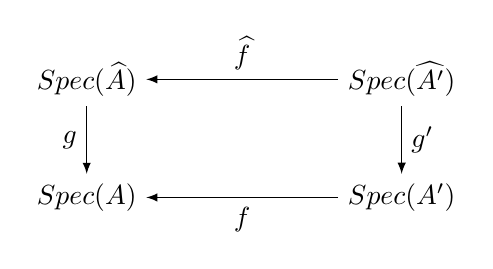
\begin{tikzpicture}[>=latex]
\node (tl) at (0,1.5) {$\operatorname{Spec}(\widehat A)$};
\node (tr) at (4,1.5) {$\operatorname{Spec}(\widehat{A'})$};
\node (bl) at (0,0) {$\operatorname{Spec}(A)$};
\node (br) at (4,0) {$\operatorname{Spec}(A')$};
\draw[->] (tr) -- node[above] {$\widehat f$} (tl);
\draw[->] (tl) -- node[left] {$g$} (bl);
\draw[->] (tr) -- node[right] {$g'$} (br);
\draw[->] (br) -- node[below] {$f$} (bl);
\end{tikzpicture}
\]
où $g$ et $g'$ sont les morphismes canoniques. Comme par hypothèse $f$ est
un $\boldsymbol P$-morphisme et $g'$ un morphisme régulier, il résulte de
$(\mathrm P_{\mathrm I})$ que $f\circ g'=g\circ\widehat f$ est un
$\boldsymbol P$-morphisme. D'autre part, l'hypothèse que $f$ est un
$\boldsymbol P$-morphisme implique que $f$ est plat, donc il en est de même
de $\widehat f$ (Bourbaki, \emph{Alg. comm.}, chap. III, \S~5,
n\textsuperscript{o}~4, cor. de la prop. 3), qui est d'ailleurs un
homomorphisme local, donc fidèlement plat (0$_{\mathrm I}$, 6.6.2); il
résulte alors de $(\mathrm P_{\mathrm{II}})$ que $g$ est un
$\boldsymbol P$-morphisme.
\end{proof}

\begin{corollary}[7.4.3]
\label{IV.2.s7.4.3-fr}
\begin{enumerate}
\item[\emph{(i)}] Soient $A$ un $\boldsymbol P$-anneau local noethérien,
$A'=\widehat A$ son complété. Supposons que pour tout idéal premier
$\mathfrak p'$ de $A'$, les fibres formelles de $A'_{\mathfrak p'}$ soient
géométriquement régulières; alors, pour tout idéal premier $\mathfrak p$ de
$A$, $A_{\mathfrak p}$ est un $\boldsymbol P$-anneau.
\item[\emph{(ii)}] Supposons que $\boldsymbol P$ vérifie la condition
$(\mathrm P_{\mathrm{IV}})$ (7.3.6). Soient $A$ un $\boldsymbol P$-anneau
local noethérien, $B$ une $A$-algèbre locale essentiellement de type fini,
et telle que l'homomorphisme $A\to B$ soit local. Posons $A'=\widehat A$,
et soit $\mathfrak n'$ l'unique idéal premier de
$B'=B\otimes_A A'$ au-dessus de l'idéal maximal de $B$ et de l'idéal
maximal de $A'$. Si les fibres formelles de $B'_{\mathfrak n'}$ sont
géométriquement régulières, alors $B$ est un $\boldsymbol P$-anneau.
\end{enumerate}
\end{corollary}

\begin{proof}
\begin{enumerate}
\item[\emph{(i)}] Comme par hypothèse
$\operatorname{Spec}(A')\to\operatorname{Spec}(A)$ est un
$\boldsymbol P$-morphisme, il en est de même de
$\operatorname{Spec}(A'_{\mathfrak p'})\to
\operatorname{Spec}(A_{\mathfrak p})$ en vertu de (7.3.2, b)), pour tout
idéal premier $\mathfrak p$ de $A$ et tout idéal premier $\mathfrak p'$ de
$A'$ au-dessus de $\mathfrak p$. Il suffit alors d'appliquer le lemme
(7.4.2) à ce morphisme, en remarquant que le morphisme
$\operatorname{Spec}(A')\to\operatorname{Spec}(A)$ est surjectif.
\item[\emph{(ii)}] En vertu de (7.4.2), il suffit de prouver que le morphisme
$\operatorname{Spec}(B'_{\mathfrak n'})\to\operatorname{Spec}(B)$ est un
$\boldsymbol P$-morphisme. Or on a $B=C_{\mathfrak n}$, où $C$ est une
$A$-algèbre de type fini et $\mathfrak n$ un idéal premier de $C$ au-dessus
de l'idéal maximal de $A$. Si on pose $C'=C\otimes_A A'$, il résulte des
hypothèses et de (7.3.7) que
$\operatorname{Spec}(C')\to\operatorname{Spec}(C)$ est un
$\boldsymbol P$-morphisme; comme $B'_{\mathfrak n'}$ est un anneau local en
un idéal premier de $C'$ au-dessus de $\mathfrak n$, la conclusion résulte
de (7.3.2, b)).
\end{enumerate}
\end{proof}

\begin{theorem}[7.4.4]
\label{IV.2.s7.4.4-fr}
Les hypothèses sur $\boldsymbol P$ étant celles de (7.4.1), soit $A$ un
$\boldsymbol P$-anneau local noethérien.
\begin{enumerate}
\item[\emph{(i)}] Pour tout idéal premier $\mathfrak p$ de $A$,
$A_{\mathfrak p}$ est un $\boldsymbol P$-anneau.
\item[\emph{(ii)}] Supposons en outre que $\boldsymbol P$ vérifie la condition
$(\mathrm P_{\mathrm{IV}})$. Alors tout anneau local qui est une
$A$-algèbre essentiellement de type fini est un $\boldsymbol P$-anneau.
\end{enumerate}
\end{theorem}

\begin{proof}
\begin{enumerate}
\item[\emph{(i)}] Appliquant (7.4.3, (i)), tout revient à voir que pour tout
idéal premier $\mathfrak p'$ de $A'=\widehat A$,
$A'_{\mathfrak p'}$ a ses fibres formelles géométriquement régulières. Or,
cela a été démontré dans (0, 22.3.3 et 22.5.8).

\oldpage[IV-2]{200}

\item[\emph{(ii)}] Soit $B$ une $A$-algèbre essentiellement de type fini qui
soit un anneau local; si $\mathfrak p$ est l'idéal premier de $A$ au-dessus
duquel est l'idéal maximal de $B$, $B$ est aussi une
$A_{\mathfrak p}$-algèbre essentiellement de type fini (1.3.8); en vertu de
(i), on peut donc supposer que $\mathfrak p$ est l'idéal maximal $\mathfrak m$
de $A$. On a donc $B=C_{\mathfrak q}$, où $C$ est une $A$-algèbre de type
fini, $\mathfrak q$ un idéal premier de $C$ au-dessus de $\mathfrak m$; soit
$\mathfrak n\supset\mathfrak q$ un idéal maximal de $C$ (nécessairement
au-dessus de $\mathfrak m$); si l'on pose $k=A/\mathfrak m$,
$C/\mathfrak mC$ est une $k$-algèbre de type fini, donc le corps résiduel
$k'$ de $C$ en l'idéal maximal $\mathfrak n$ est fini sur $k$ (I, 6.4.2);
en vertu de (i), il suffira de prouver que $C_{\mathfrak n}$ est un
$\boldsymbol P$-anneau, puisque $C_{\mathfrak q}$ est un anneau local en un
idéal premier de $C_{\mathfrak n}$. On est ainsi ramené à démontrer le
lemme suivant.
\end{enumerate}
\end{proof}

\begin{lemma}[7.4.4.1]
\label{IV.2.s7.4.4.1-fr}
Soient $A$ un $\boldsymbol P$-anneau local noethérien, $k$ son corps
résiduel, $C$ une $A$-algèbre de type fini, $B$ un anneau local en un idéal
premier $\mathfrak n$ de $C$, tel que : 1\textsuperscript{o}
l'homomorphisme $A\to B$ soit local; 2\textsuperscript{o} le corps résiduel
$k'$ de $B$ soit une extension finie de $k$. Si $\boldsymbol P$ satisfait à
$(\mathrm P_{\mathrm{IV}})$, $B$ est un $\boldsymbol P$-anneau.
\end{lemma}

\begin{proof}
Soit $(x_i)_{1\leqslant i\leqslant m}$ un système de générateurs de la
$A$-algèbre $C$; montrons d'abord que l'on peut raisonner par récurrence sur
$m$. Soit $C'$ la sous-algèbre de $C$ engendrée par
$x_1,\ldots,x_{m-1}$, et soit $\mathfrak n'=\mathfrak n\cap C'$.
L'homomorphisme $A\to C_{\mathfrak n}$ se factorise en
$A\to C'_{\mathfrak n'}\to C_{\mathfrak n}$ et il est clair que
$A\to C'_{\mathfrak n'}$ et $C'_{\mathfrak n'}\to C_{\mathfrak n}$ sont
des homomorphismes locaux; si $k''$ est le corps résiduel de
$C'_{\mathfrak n'}$, $k\to k'$ se factorise de même en
$k\to k''\to k'$, donc $k''$ est extension finie de $k$ et $k'$ extension
finie de $k''$. L'hypothèse de récurrence entraîne que
$C'_{\mathfrak n'}$ est un $\boldsymbol P$-anneau; en outre, si
$S'=C'-\mathfrak n'$, $C_{\mathfrak n}$ est un anneau local de
$S'^{-1}C$; comme $C=C'[x_m]$, on a
$S'^{-1}C=C'_{\mathfrak n'}[x_m/1]$ et l'hypothèse de récurrence montre
encore que $C_{\mathfrak n}$ est un $\boldsymbol P$-anneau. On est ainsi
ramené au cas où $C$ est une $A$-algèbre engendrée par un \emph{seul}
élément $t$.

Appliquons (7.4.3, (ii)); en posant $A'=\widehat A$,
$B'=B\otimes_A A'$ est un anneau local de $C\otimes_A A'$ en un idéal
premier au-dessus de $\mathfrak n$; comme $A$ et $A'$ ont même corps
résiduel $k$, le corps résiduel de $C\otimes_A A'$ en cet idéal premier est
égal à $k'$. D'ailleurs $C\otimes_A A'$ est une $A'$-algèbre engendrée par
un seul élément. Il résulte donc de (7.4.3, (ii)) qu'on peut se borner à
démontrer (7.4.4.1) lorsque $\boldsymbol P$ est la propriété (iv$'$) de
(7.3.8), que $A$ est \emph{complet} et $C$ engendrée par un seul élément
$t$.

Pour montrer que les fibres formelles de $B=C_{\mathfrak n}$ sont alors
géométriquement régulières, appliquons le critère (7.3.16, b)). Soit $B_1$
une $B$-algèbre finie \emph{intègre}, donc engendrée par un nombre fini
d'éléments entiers sur $B$. En multipliant ces éléments par un élément de
$S=C-\mathfrak n$, on peut supposer qu'ils sont entiers sur $C$, et on peut
donc écrire $B_1=S^{-1}C_1$, où $C_1$ est une sous-$C$-algèbre de $B_1$
engendrée par un nombre fini d'éléments entiers sur $C$, donc une
$C$-algèbre \emph{finie et intègre}. D'autre part, $B_1$ est un anneau
semi-local, et tout anneau local $B_2$ de $B_1$ en un idéal maximal est un
anneau local de $C_1$ en un idéal premier, tel que $A\to B_2$ soit un
homomorphisme local; en outre, le corps résiduel de $B_2$ est une extension
finie de $k'$, donc de $k$. On voit donc (compte tenu de (7.3.14) et de (i))
qu'on est ramené à la question suivante : soit $C$ un anneau noethérien
\emph{intègre}, contenant un sous-anneau $C_0$ qui est une $A$-algèbre
engendrée par un seul élément $t$ et telle que $C$ soit une $C_0$-algèbre
\emph{finie}; si $\mathfrak n$ est un idéal maximal de $C$

\oldpage[IV-2]{201}

au-dessus de l'idéal maximal de $A$, et $B=C_{\mathfrak n}$, il s'agit de
montrer que pour tout idéal premier $\mathfrak q$ de $\widehat B$, dont
l'image réciproque dans $B$ est 0, l'anneau
$\widehat B_{\mathfrak q}$ est \emph{régulier}. On peut d'ailleurs remplacer
$A$ par son image dans $C$, qui est un anneau local complet (comme quotient
de $A$) et intègre. La conclusion à prouver est alors conséquence du lemme
suivant, plus général en apparence.
\end{proof}

\begin{lemma}[7.4.4.2]
\label{IV.2.s7.4.4.2-fr}
Soient $A$ un anneau local noethérien intègre et complet, $k$ son corps
résiduel, $C$ un anneau intègre contenant $A$, tel qu'il existe $t\in C$
pour lequel $C$ soit une $A[t]$-algèbre finie. Soit $\mathfrak n$ un idéal
maximal de $C$ au-dessus de l'idéal maximal $\mathfrak m$ de $A$; posons
$B=C_{\mathfrak n}$, $X=\operatorname{Spec}(B)$,
$B'=\widehat B$, $X'=\operatorname{Spec}(\widehat B)$; si
$U=\operatorname{Reg}(X)$, $U'=\operatorname{Reg}(X')$, et si
$f:X'\to X$ est le morphisme canonique, on a alors
$f^{-1}(U)\subset U'$.
\end{lemma}

\begin{proof}
L'assertion à démontrer pour obtenir (7.4.4.1) se déduira de ce lemme en
observant que, puisque $B$ est intègre, le point générique de $X$ appartient
à $U$.

On notera que puisque $C$ est une $A$-algèbre de type fini, et $\mathfrak n$
un idéal maximal de $C$, le corps résiduel $k'$ de
$C_{\mathfrak n}=B$ (donc aussi de $B'$) est une extension finie de $k$
(I, 6.4.11 et 6.4.2).

Si l'on pose $Y=\operatorname{Spec}(C)$, il résulte de (6.12.8) que
$\operatorname{Reg}(Y)$ est ouvert dans $Y$; comme les anneaux locaux de
$X$ sont des anneaux locaux de $Y$ (I, 2.4.2), on a
$U=X\cap\operatorname{Reg}(Y)$, donc $U$ est ouvert dans $X$; d'autre part
(6.12.7) $U'$ est ouvert dans $X'$, donc $S'=X'-U'$ est fermé; par suite
$S'\cap f^{-1}(U)$ est localement fermé dans $X'$, et tout revient à
prouver que cet ensemble est vide. On sait (5.1.10) que dans le cas
contraire, il existerait dans $S'\cap f^{-1}(U)$ un idéal premier
$\mathfrak p'$ tel que $\dim(B'/\mathfrak p')\leqslant1$. Remarquons d'abord
que $\mathfrak p'$ ne peut être l'idéal maximal $\mathfrak mB'$ de $B'$,
où $\mathfrak m$ est l'idéal maximal de $B$. En effet, cela signifierait que
$B=B_{\mathfrak m}$ serait régulier, donc aussi $B'=\widehat B$ (0,
17.1.5), et on aurait par suite $\mathfrak mB'\in U'$ contrairement à
l'hypothèse. On doit donc avoir $\dim(B'/\mathfrak p')=1$. Posons
$\mathfrak p=B\cap\mathfrak p'$; par hypothèse $B_{\mathfrak p}$ est
régulier, mais $B'_{\mathfrak p'}$ ne l'est pas; comme
$B'_{\mathfrak p'}$ est un $B_{\mathfrak p}$-module plat, il résulte de
(6.5.2) que la fibre $Z$ de $f$ au point $\mathfrak p$ n'est pas régulière
au point $\mathfrak p'$. Montrons qu'on peut se ramener au cas où
$\mathfrak p=0$. En effet, dans le cas général, si l'on pose
$\mathfrak q=\mathfrak p\cap C$, $\mathfrak r=\mathfrak p\cap A$,
$C/\mathfrak q$ est une $(A/\mathfrak r)[\bar t]$-algèbre finie (où
$\bar t$ est la classe de $t$ mod. $\mathfrak q$); comme
$\mathfrak p=\mathfrak qB$, $B/\mathfrak p$ est égal à
$(C/\mathfrak q)_{\mathfrak n/\mathfrak q}$, et
$\mathfrak n/\mathfrak q$ est un idéal maximal de $C/\mathfrak q$
au-dessus de l'idéal maximal $\mathfrak m/\mathfrak r$ de
$A/\mathfrak r$; on voit donc que les hypothèses de (7.4.4.2) sont encore
remplies par $A/\mathfrak r$, $C/\mathfrak q$ et $B/\mathfrak p$, et comme
le complété de $B/\mathfrak p$ est $B'/\mathfrak pB'$, cela prouve notre
assertion. Supposons donc $\mathfrak p=0$, de sorte que $Z$ est la fibre
générique et que l'homomorphisme $B\to B'/\mathfrak p'$ est injectif.
Posons $V=B'/\mathfrak p'$, et distinguons deux cas :

\emph{I) $V$ est une $A$-algèbre finie.} --- Comme $B\subset V$, $B$ est
\emph{a fortiori} une $A$-algèbre finie, et comme $A$ est complet, il en est
de même de $B$ (Bourbaki, \emph{Alg. comm.}, chap. IV, \S~2,
n\textsuperscript{o}~5, cor. 3 de la prop. 9), d'où $B'=B$,
$\mathfrak p'=0$, donc $B'_{\mathfrak p'}$ est un corps, et par suite un
anneau régulier, contrairement à l'hypothèse.

\emph{II) $V$ n'est pas une $A$-algèbre finie.} --- Comme l'anneau local
$A$ est complet, cela implique que $V$ n'est pas une $A$-algèbre
quasi-finie (0$_{\mathrm I}$, 7.4.1 et 7.4.2); mais par hypothèse le corps
résiduel $k'$ de $V$ est extension finie du corps résiduel $k$ de $A$,

\oldpage[IV-2]{202}

donc (0$_{\mathrm I}$, 7.4.4) l'idéal $\mathfrak mV$ n'est pas un idéal de
définition de $V$. Comme $V$ est un anneau local intègre noethérien de
dimension 1, 0 est le seul idéal de $V$ qui ne soit pas un idéal de
définition, donc $\mathfrak mV=0$. Mais on a $A\subset V$ et $V$ est
intègre, d'où $\mathfrak m=0$ et $A=k$ est un corps. On en déduit tout
d'abord $\dim(C)\leqslant1$ (0, 16.1.5); mais comme $\dim(V)=1$, les
relations
\[
\dim(V)\leqslant\dim(B')=\dim(B)\leqslant\dim(C)
\]
montrent que cela entraîne
$\dim(C)=\dim(B)=\dim(B')=\dim(B'/\mathfrak p')=1$, et par suite
$\mathfrak p'$ est nécessairement un idéal premier minimal de $B'$. Nous
arriverons donc encore à une contradiction si nous prouvons que
$B'_{\mathfrak p'}$ est un corps, ou encore que l'anneau $B'$ est réduit.
Or, comme $C$ est une $k$-algèbre de type fini, la clôture intégrale $C_1$
de $C$ est une $C$-algèbre finie (Bourbaki, \emph{Alg. comm.}, chap. V,
\S~3, n\textsuperscript{o}~2, th. 2); si l'on pose
$S=C-\mathfrak n$, $B_1=S^{-1}C_1$ est la clôture intégrale de $B$, donc
$B_1$ est une $B$-algèbre finie, et par suite un anneau semi-local
noethérien, intègre et intégralement clos et de dimension 1 (0, 16.1.5); si
$\mathfrak m_j$ $(1\leqslant j\leqslant h)$ sont ses idéaux maximaux, les
$(B_1)_{\mathfrak m_j}$ sont donc des anneaux de valuation discrète (II,
7.1.6), et le complété $B'_1$ de $B_1$ est le composé direct des anneaux de
valuation discrète complétés des $(B_1)_{\mathfrak m_j}$ (Bourbaki,
\emph{Alg. comm.}, chap. III, \S~2, n\textsuperscript{o}~13, prop. 18);
$B'_1$ est donc réduit, et comme le complété $B'$ de $B$ est un
sous-anneau de $B'_1$ (Bourbaki, \emph{Alg. comm.}, chap. IV, \S~2,
n\textsuperscript{o}~5, cor. 3 de la prop. 9), c'est aussi un anneau réduit.
C.Q.F.D.
\end{proof}

\begin{corollary}[7.4.5]
\label{IV.2.s7.4.5-fr}
Supposons que la propriété $\boldsymbol P$ satisfasse aux conditions
$(\mathrm P_{\mathrm I})$, $(\mathrm P_{\mathrm{II}})$,
$(\mathrm P_{\mathrm{III}})$. Soit $A$ un anneau noethérien. Les conditions
suivantes sont équivalentes :
\begin{enumerate}
\item[\emph{a)}] Pour tout idéal premier $\mathfrak p$ de $A$,
$A_{\mathfrak p}$ est un $\boldsymbol P$-anneau.
\item[\emph{b)}] Pour tout idéal maximal $\mathfrak m$ de $A$,
$A_{\mathfrak m}$ est un $\boldsymbol P$-anneau.
\end{enumerate}
Si de plus $\boldsymbol P$ satisfait à $(\mathrm P_{\mathrm{IV}})$, les
propriétés a) et b) sont aussi équivalentes à :
\begin{enumerate}
\item[\emph{c)}] Pour toute $A$-algèbre de type fini $B$ et tout idéal
premier $\mathfrak q$ de $B$, $B_{\mathfrak q}$ est un
$\boldsymbol P$-anneau.
\end{enumerate}
\end{corollary}

\begin{proof}
L'équivalence de a) et b) résulte de (7.4.4, (i)), et celle de a) et c) de
(7.4.4, (ii)).

Lorsque la condition a) de (7.4.5) est remplie, on dit que $A$ est un
$\boldsymbol P$-anneau; pour les anneaux semi-locaux noethériens, cette
définition coïncide avec celle de (7.3.13), lorsque les conditions
$(\mathrm P_{\mathrm I})$, $(\mathrm P_{\mathrm{II}})$ et
$(\mathrm P_{\mathrm{III}})$ sont satisfaites. L'anneau $\mathbf Z$ est un
$\boldsymbol P$-anneau (7.3.19, (iv)); tout anneau local complet est un
$\boldsymbol P$-anneau.
\end{proof}

\begin{proposition}[7.4.6]
\label{IV.2.s7.4.6-fr}
Supposons que la propriété $\boldsymbol P$ satisfasse aux conditions
$(\mathrm P_{\mathrm I})$, $(\mathrm P_{\mathrm{II}})$ et
$(\mathrm P_{\mathrm{III}})$. Soient $A$ un anneau noethérien,
$\mathfrak J$ un idéal de $A$, $\widehat A$ le séparé complété de $A$ pour
la topologie $\mathfrak J$-préadique. Alors, si $A$ est un
$\boldsymbol P$-anneau (7.4.5), le morphisme canonique
$\operatorname{Spec}(\widehat A)\to\operatorname{Spec}(A)$ est un
$\boldsymbol P$-morphisme.
\end{proposition}

\begin{proof}
En utilisant (7.3.2, c$'$)), il suffit de prouver que pour tout idéal
maximal $\mathfrak n$ de $\widehat A$, d'image réciproque $\mathfrak m$
dans $A$, le morphisme
$\operatorname{Spec}((\widehat A)_{\mathfrak n})\to
\operatorname{Spec}(A_{\mathfrak m})$ est un $\boldsymbol P$-morphisme.
On sait (Bourbaki, \emph{Alg. comm.}, chap. III, \S~3,
n\textsuperscript{o}~4, prop. 8) que l'homomorphisme canonique
$A_{\mathfrak m}\to(\widehat A)_{\mathfrak n}$ est injectif, que la
topologie $\mathfrak mA_{\mathfrak m}$-préadique sur $A_{\mathfrak m}$ est
induite par la topologie
$\mathfrak n(\widehat A)_{\mathfrak n}$-préadique et que
$A_{\mathfrak m}$ est dense dans $(\widehat A)_{\mathfrak n}$ pour cette
topologie, de sorte que le complété de $A_{\mathfrak m}$ pour la topologie
$\mathfrak mA_{\mathfrak m}$-préadique s'identifie à celui de
$(\widehat A)_{\mathfrak n}$ pour la topologie
$\mathfrak n(\widehat A)_{\mathfrak n}$-préadique. On a donc deux morphismes
\[
\operatorname{Spec}(\widehat{A_{\mathfrak m}})
\xrightarrow{f}\operatorname{Spec}((\widehat A)_{\mathfrak n})
\xrightarrow{g}\operatorname{Spec}(A_{\mathfrak m})
\]

\oldpage[IV-2]{203}

tels que $f$ soit fidèlement plat; comme par hypothèse $g\circ f$ est un
$\boldsymbol P$-morphisme, il en est de même de $g$ en vertu de
$(\mathrm P_{\mathrm{II}})$.
\end{proof}

\begin{corollary}[7.4.7]
\label{IV.2.s7.4.7-fr}
Supposons que $\boldsymbol P$ vérifie les conditions
$(\mathrm P_{\mathrm I})$, $(\mathrm P'_{\mathrm I})$,
$(\mathrm P_{\mathrm{II}})$, $(\mathrm P_{\mathrm{III}})$ et
$(\mathrm P_{\mathrm{IV}})$. Alors, si $A$ est un
$\boldsymbol P$-anneau (7.4.5), le morphisme canonique
$\operatorname{Spec}(A[[T_1,\ldots,T_r]])\to\operatorname{Spec}(A)$ est un
$\boldsymbol P$-morphisme. En particulier, si de plus $A$ est intègre, $K$
son corps des fractions, et si $\mathfrak p$ est un idéal premier de
$B=A[[T_1,\ldots,T_r]]$ tel que $\mathfrak p\cap A=0$, alors la propriété
$\boldsymbol P(B_{\mathfrak p},K)$ est vraie.
\end{corollary}

\begin{proof}
En effet, le morphisme canonique
$\operatorname{Spec}(B)\to\operatorname{Spec}(A)$ se factorise en
\[
\operatorname{Spec}(A[[T_1,\ldots,T_r]])
\xrightarrow{f}\operatorname{Spec}(A[T_1,\ldots,T_r])
\xrightarrow{g}\operatorname{Spec}(A).
\]
Il est clair que le morphisme $g$ est régulier (0, 17.3.7); en vertu de
(7.4.5), $A[T_1,\ldots,T_r]$ est un $\boldsymbol P$-anneau, donc il résulte
de (7.4.6) que $f$ est un $\boldsymbol P$-morphisme; comme $g$ est régulier,
donc est aussi un $\boldsymbol P$-morphisme (7.3.5, (i)), il en est de même
de $g\circ f$ en vertu de $(\mathrm P'_{\mathrm I})$.

On notera que la conclusion est encore valable si au lieu de supposer que
$\boldsymbol P$ vérifie $(\mathrm P'_{\mathrm I})$ et que tout morphisme
régulier est un $\boldsymbol P$-morphisme, on suppose seulement qu'un
morphisme composé $g\circ f$ est un $\boldsymbol P$-morphisme lorsque $g$
est régulier et $f$ un $\boldsymbol P$-morphisme (condition symétrique en
quelque sorte de $(\mathrm P'_{\mathrm I})$).
\end{proof}

\begin{remark}[7.4.8]
\label{IV.2.s7.4.8-fr}
Les résultats précédents posent les problèmes suivants :
\begin{enumerate}
\item[\emph{A)}] Soit $A$ un anneau de Zariski \emph{complet}, et soit
$\mathfrak J$ un idéal de définition de $A$; si l'anneau $A/\mathfrak J$
est un $\boldsymbol P$-anneau, en est-il de même de $A$? Il en résulterait
que pour tout $\boldsymbol P$-anneau noethérien $A$ et tout idéal
$\mathfrak J$ de $A$, le séparé complété $\widehat A$ pour la topologie
$\mathfrak J$-préadique serait aussi un $\boldsymbol P$-anneau.
\item[\emph{B)}] Soit $k$ un corps valué complet non discret; on appelle
encore anneau des \emph{séries formelles restreintes}
$k\{T_1,\ldots,T_n\}$ le sous-anneau de l'anneau de séries formelles
$k[[T_1,\ldots,T_n]]$ formées des séries dont les coefficients \emph{tendent
vers 0}. Un tel anneau est-il un $\boldsymbol P$-anneau?
\item[\emph{C)}] Si $A$ est un $\boldsymbol P$-anneau linéairement
topologisé, $S$ une partie multiplicative de $A$, les anneaux
$A\{S^{-1}\}$ (0$_{\mathrm I}$, 7.6.1) et $A_{\{S\}}$
(0$_{\mathrm I}$, 7.6.15) sont-ils des $\boldsymbol P$-anneaux?
\end{enumerate}
\end{remark}

\subsection{Un critère pour les $\boldsymbol P$-morphismes}
\label{subsection:IV.7.5-fr}

\begin{env}[7.5.0]
\label{IV.2.s7.5.0-fr}
Ce numéro ne sera pas utilisé dans la suite du chapitre IV, et peut donc être
omis en première lecture. Nous verrons d'ailleurs plus loin (7.9.8) que les
résultats du présent numéro peuvent être considérablement améliorés quand on
dispose de la « résolution des singularités ».

Dans la suite de ce numéro, nous considérerons une propriété
$\boldsymbol R(A)$, et nous désignerons par $\boldsymbol P(Z,k)$ la propriété
suivante :
\begin{quote}
« $Z$ est un préschéma localement noethérien sur un corps $k$, et, pour toute
extension finie $k'$ de $k$, si l'on pose $Z'=Z\otimes_k k'$, la propriété
$\boldsymbol R(\mathscr O_{Z',z'})$ est vraie pour tout $z'\in Z'$. »
\end{quote}
\end{env}

\begin{theorem}[7.5.1]
\label{IV.2.s7.5.1-fr}
Soient $A$, $B$ deux anneaux locaux noethériens complets, $\mathfrak m$
l'idéal maximal de $A$, $k=A/\mathfrak m$ son corps résiduel,
$\varphi:A\to B$ un homomorphisme local tel que :
\begin{enumerate}
\item[\emph{(i)}] Le corps résiduel de $B$ est une extension finie de $k$.
\item[\emph{(ii)}] $B$ est un $A$-module plat.
\end{enumerate}
Soit d'autre part $\boldsymbol R(C)$ une propriété vérifiant la condition
$(\mathrm R_{\mathrm{III}})$ (7.3.18) et la condition suivante :
\begin{quote}
$(\mathrm R_{\mathrm{IV}})$ Pour tout anneau local $C$ en un idéal premier
d'un anneau local noethérien complet et tout élément $C$-régulier $t$ dans
l'idéal maximal de $C$, la propriété $\boldsymbol R(C/tC)$ implique
$\boldsymbol R(C)$.
\end{quote}

\oldpage[IV-2]{204}

Cela étant, soit $f={}^a\varphi:\operatorname{Spec}(B)\to
\operatorname{Spec}(A)$, et supposons que la propriété
$\boldsymbol P(\operatorname{Spec}(B\otimes_A k),k)$ soit vraie. Alors, pour
tout $x\in\operatorname{Spec}(A)$ la propriété
$\boldsymbol P(f^{-1}(x),k(x))$ est vraie.
\end{theorem}

\begin{proof}
Autrement dit, la propriété $\boldsymbol P$ pour la fibre du point fermé de
$\operatorname{Spec}(A)$ entraîne cette même propriété pour toutes les
fibres du morphisme $f$ (c'est-à-dire que $f$ est un
$\boldsymbol P$-morphisme (7.3.1)). Nous procéderons en plusieurs étapes :

\emph{I) Réduction à l'étude des anneaux locaux de la fibre générique.} ---
Appliquons le lemme (7.3.16.2) : il suffit de voir que pour toute
$A$-algèbre finie et intègre $A'$, de corps des fractions $K'$, si l'on
pose $B'=B\otimes_A A'$, tous les anneaux locaux de
$\operatorname{Spec}(B'\otimes_{A'}K')$ vérifient la propriété
$\boldsymbol R$. L'anneau $A'$ (resp. $B'$) est semi-local complet ($B'$
étant une $B$-algèbre finie), donc produit d'anneaux locaux complets; comme
$A'$ est supposé intègre, il est local; tout idéal maximal $\mathfrak n'$ de
$B'$ est au-dessus de l'idéal maximal $\mathfrak n$ de $B$, donc au-dessus
de $\mathfrak m$, et par suite son image réciproque dans $A'$ est l'idéal
maximal $\mathfrak m'$ de $A'$. Comme tout anneau local de
$\operatorname{Spec}(B'\otimes_{A'}K')$ est un anneau local de
$\operatorname{Spec}(B')$, donc de l'un des
$\operatorname{Spec}(B'_{\mathfrak n'})$ (au-dessus du point générique de
$A'$), on voit qu'il suffira de prouver que les anneaux locaux de
\[
\operatorname{Spec}(B'_{\mathfrak n'}\otimes_{A'}K')
\]
possèdent la propriété $\boldsymbol R$. Or $A'$ et
$B'_{\mathfrak n'}$ sont des anneaux locaux noethériens complets; le corps
résiduel de $B'_{\mathfrak n'}$ est extension finie de celui de $B$, donc
aussi de $k$, et \emph{a fortiori} du corps résiduel $k'$ de $A'$; cette
remarque et (2.1.4) montrent que $A'$ et $B'_{\mathfrak n'}$ vérifient les
conditions (i) et (ii) de l'énoncé. D'autre part, si $k''$ est une extension
finie de $k'$, $k''$ est aussi extension finie de $k$, et les anneaux locaux
de
\[
\operatorname{Spec}(B'_{\mathfrak n'}\otimes_{A'}k'')
\]
sont aussi des anneaux locaux de $\operatorname{Spec}(B\otimes_A k'')$;
donc l'hypothèse que
$\boldsymbol P(\operatorname{Spec}(B\otimes_A k),k)$ est vraie entraîne que
\[
\boldsymbol P(\operatorname{Spec}(B'_{\mathfrak n'}\otimes_{A'}k'),k')
\]
est vraie.

On est ainsi ramené au cas où $A$ est de plus supposé intègre, de corps des
fractions $K$, et à prouver que les anneaux locaux de
$\operatorname{Spec}(B\otimes_A K)$ possèdent la propriété
$\boldsymbol R$.

\emph{II) Cas où $\dim(A)=1$.} --- Soit $A'$ la clôture intégrale de $A$;
on sait (0, 23.1.6) que $A'$ est une $A$-algèbre finie et un anneau local
complet; si l'on pose $B'=B\otimes_A A'$, on a
$B\otimes_A K=B'\otimes_{A'}K$. Le même raisonnement que dans I) montre
qu'il suffit, pour tout idéal maximal $\mathfrak n'$ de $B'$, de prouver que
les anneaux locaux de
$B'_{\mathfrak n'}\otimes_{A'}K$ vérifient $\boldsymbol R$; en outre, ce
raisonnement montre aussi que $A'$ et $B'_{\mathfrak n'}$ vérifient les
hypothèses (i) et (ii) de l'énoncé et que
$\boldsymbol P(\operatorname{Spec}(B'_{\mathfrak n'}\otimes_{A'}k'),k')$
est vraie ($k'$ étant le corps résiduel de $A'$). En outre, comme
$\dim(A')=1$ (0, 16.1.5) et que $A'$ est intègre et intégralement clos,
c'est un anneau de valuation discrète complet. On peut donc se borner au
cas où $A$ est déjà un anneau de valuation discrète complet; si alors $u$
est une uniformisante de $A$, le fait que $u$ soit $A$-régulier et que $B$
soit un $A$-module plat entraîne que $t=\varphi(u)$ est un élément
$B$-régulier, qui appartient à l'idéal maximal de $B$. L'hypothèse que
$\boldsymbol P(\operatorname{Spec}(B\otimes_A k),k)$ est vraie entraîne en
particulier que $\boldsymbol R(B/tB)$ est vraie; en vertu de
$(\mathrm R_{\mathrm{IV}})$, $\boldsymbol R(B)$ est donc vraie. Autrement
dit, $U_{\boldsymbol R}(\operatorname{Spec}(B))$ contient le point fermé de
$\operatorname{Spec}(B)$. Mais comme
$U_{\boldsymbol R}(\operatorname{Spec}(B))$ est ouvert en vertu de
$(\mathrm R_{\mathrm{III}})$ et que $\operatorname{Spec}(B)$ est le seul
ensemble ouvert de $\operatorname{Spec}(B)$ contenant le point fermé, tous
les anneaux locaux de $\operatorname{Spec}(B)$ possèdent la propriété
$\boldsymbol R$, et en particulier ceux de
$\operatorname{Spec}(B\otimes_A K)$.

\emph{III) Cas général.} --- Le cas $\dim(A)=0$ est trivial, puisqu'alors
$A=k$; on peut donc se borner au cas où $\dim(A)\geqslant1$. On sait
(6.12.7) que $\operatorname{Spec}(A)$ contient un ouvert non vide $V$ dont
tous les points sont réguliers; comme $\dim(A)\geqslant1$, l'intersection
$V'$ de $V$ et du complémentaire du point fermé de
$\operatorname{Spec}(A)$ est un ouvert non vide, contenant donc le point
générique de $\operatorname{Spec}(A)$. Si nous prouvons que
\[
f^{-1}(V')\subset U_{\boldsymbol R}(\operatorname{Spec}(B)),
\]
la proposition sera démontrée \emph{a fortiori}. Autrement dit, il suffit de
voir que l'ensemble $Z$, intersection de $f^{-1}(V')$ et du complémentaire
de $U_{\boldsymbol R}(\operatorname{Spec}(B))$, est vide. Raisonnons par
l'absurde : comme, en vertu de $(\mathrm R_{\mathrm{III}})$,
$U_{\boldsymbol R}(\operatorname{Spec}(B))$ est ouvert dans
$\operatorname{Spec}(B)$, $Z$ est localement fermé dans
$\operatorname{Spec}(B)$; s'il n'était pas vide, il contiendrait un point
$x$ tel que $\dim(\overline{\{x\}})\leqslant1$ (5.1.10); comme
$f(x)\in V'$ est distinct du point fermé de $\operatorname{Spec}(A)$, $x$
est distinct du point fermé de $\operatorname{Spec}(B)$, autrement dit
$\dim(\overline{\{x\}})=1$. Nous allons prouver que cela est impossible,
autrement dit que, si $\dim(\overline{\{x\}})=1$ et $f(x)\in V'$ alors on a
$\boldsymbol R(\mathscr O_x)$. En d'autres termes, il s'agit de voir que,
si $\mathfrak q$ est un idéal premier de $B$ tel que
$\dim(B/\mathfrak q)=1$ et si $\mathfrak p=\varphi^{-1}(\mathfrak q)$ est
distinct de $\mathfrak m$ et tel que $A_{\mathfrak p}$ soit régulier, alors
on a $\boldsymbol R(B_{\mathfrak q})$. Comme
$\mathfrak p\ne\mathfrak m$, $\mathfrak m(B/\mathfrak q)$ n'est pas réduit
à 0, donc est un idéal de définition de l'anneau local intègre
$B/\mathfrak q$ de dimension 1; d'autre part, en vertu de (i), le corps
résiduel de $B/\mathfrak q$ est une extension finie du corps résiduel $k$
de $A/\mathfrak p$, donc $B/\mathfrak q$ est une
$(A/\mathfrak p)$-algèbre quasi-finie (0$_{\mathrm I}$, 7.4.4). Mais
$A/\mathfrak p$ est complet et $B/\mathfrak q$ est séparé pour la topologie
$\mathfrak m$-préadique (qui est identique à sa topologie d'anneau local);
donc (0$_{\mathrm I}$, 7.4.1), $B/\mathfrak q$ est une
$(A/\mathfrak p)$-algèbre finie. En outre, par définition,
l'homomorphisme $A/\mathfrak p\to B/\mathfrak q$ est injectif, donc (0,
16.1.5) on a
\[
\dim(A/\mathfrak p)=\dim(B/\mathfrak q)=1.
\]
On peut alors appliquer aux anneaux $A/\mathfrak p$ et
$B/\mathfrak pB$ le résultat de II), car les corps résiduels de ces anneaux
locaux sont respectivement ceux de $A$ et de $B$, et $B/\mathfrak pB$ est
un $(A/\mathfrak p)$-module plat; en outre, on a
\[
(B/\mathfrak pB)\otimes_{A/\mathfrak p}k=B\otimes_A k=B/\mathfrak mB.
\]
Par suite, les anneaux locaux de
\[
\operatorname{Spec}((B/\mathfrak pB)
\otimes_{A/\mathfrak p}k(\mathfrak p))
\]
vérifient $\boldsymbol R$. Or, $B_{\mathfrak q}/\mathfrak pB_{\mathfrak q}$
est un des anneaux locaux de
$\operatorname{Spec}((B/\mathfrak pB)
\otimes_{A/\mathfrak p}k(\mathfrak p))$. En outre,
$B_{\mathfrak q}$ est un $A_{\mathfrak p}$-module plat, et
$A_{\mathfrak p}$ est régulier. Or on a le lemme suivant.

\oldpage[IV-2]{205}

\begin{lemma}[7.5.1.1]
\label{IV.2.s7.5.1.1-fr}
Soit $\mathcal C$ une sous-catégorie pleine de la catégorie des anneaux
locaux noethériens, telle que tout anneau quotient d'un anneau de
$\mathcal C$ appartienne encore à $\mathcal C$. Soit $\boldsymbol R(C)$ une
propriété telle que si $C\in\mathcal C$ et si $t$ est un élément régulier de
l'idéal maximal de $C$ tel que $\boldsymbol R(C/tC)$ soit vraie, alors
$\boldsymbol R(C)$ est vraie.

Cela étant, soient $C$ un anneau local régulier, $k$ son corps résiduel,
$D$ un anneau local appartenant à $\mathcal C$,
$\varphi:C\to D$ un homomorphisme local faisant de $D$ un $C$-module plat.
Alors, si $\boldsymbol R(D\otimes_C k)$ est vraie, il en est de même de
$\boldsymbol R(D)$.
\end{lemma}

\begin{proof}
Raisonnons par récurrence sur $n=\dim(C)$, le lemme étant vrai par hypothèse
si $n=0$, puisqu'alors $C=k$. Soit $t$ un élément de l'idéal maximal
$\mathfrak m$ de $C$ n'appartenant pas à $\mathfrak m^2$; on sait alors que
$C/tC$ est régulier et que $\dim(C/tC)=n-1$ ((0, 17.1.8) et (0, 16.3.4)).
Comme
\[
(D/tD)\otimes_{C/tC}k=D\otimes_C k,
\]
et que $D/tD\in\mathcal C$, l'hypothèse de récurrence montre que
$\boldsymbol R(D/tD)$ est vraie; en outre, $t$ est $C$-régulier, donc aussi
$D$-régulier par platitude (0$_{\mathrm I}$, 6.3.4); l'hypothèse faite sur
$\boldsymbol R$ montre donc que $\boldsymbol R(D)$ est vraie.
\end{proof}

Pour terminer la démonstration de (7.5.1), il suffit ici d'appliquer le
lemme (7.5.1.1) en prenant pour $\mathcal C$ la catégorie des anneaux locaux
des spectres d'anneaux locaux complets, tenant compte de l'hypothèse
$(\mathrm R_{\mathrm{IV}})$, et prenant pour $C$ l'anneau
$A_{\mathfrak p}$, pour $D$ l'anneau $B_{\mathfrak q}$.
\end{proof}

\begin{corollary}[7.5.2]
\label{IV.2.s7.5.2-fr}
Soient $A$ un anneau local noethérien, $\mathfrak m$ l'idéal maximal de $A$,
$k=A/\mathfrak m$ son corps résiduel, $B$ un anneau local noethérien,
$\varphi:A\to B$ un homomorphisme local tel que :
\begin{enumerate}
\item[\emph{(i)}] Le corps résiduel de $B$ est une extension finie de $k$.
\item[\emph{(ii)}] $B$ est un $A$-module plat.
\end{enumerate}
Soit d'autre part $\boldsymbol R(C)$ une propriété vérifiant les conditions
$(\mathrm R_{\mathrm{II}})$ (7.3.10), $(\mathrm R_{\mathrm{III}})$
(7.3.18) et $(\mathrm R_{\mathrm{IV}})$ (7.5.1). Enfin, soit
$\boldsymbol R'(C)$ une propriété vérifiant la condition suivante :
\begin{quote}
$(\mathrm R_{\mathrm V})$ Si $C$, $D$ sont deux anneaux locaux noethériens,
$\psi:C\to D$ un homomorphisme local tel que
\[
g={}^a\psi:\operatorname{Spec}(D)\to\operatorname{Spec}(C)
\]
soit un $\boldsymbol P$-morphisme, alors la propriété
$\boldsymbol R'(C)$ implique $\boldsymbol R(D)$.
\end{quote}
Supposons que le morphisme canonique
$\operatorname{Spec}(\widehat A)\to\operatorname{Spec}(A)$ soit un
$\boldsymbol P'$-morphisme, où $\boldsymbol P'$ se définit à partir de
$\boldsymbol R'$ comme $\boldsymbol P$ à partir de $\boldsymbol R$ dans
(7.5.0).

Cela étant, soit
$f={}^a\varphi:\operatorname{Spec}(B)\to\operatorname{Spec}(A)$, et
supposons que la propriété
\[
\boldsymbol P(\operatorname{Spec}(\widehat B
\otimes_{\widehat A}k),k)
\]
soit vraie. Alors, pour tout $x\in\operatorname{Spec}(A)$, la propriété
$\boldsymbol P(f^{-1}(x),k(x))$ est vraie (autrement dit, $f$ est un
$\boldsymbol P$-morphisme).
\end{corollary}

\begin{proof}
Procédons encore en deux étapes :

\emph{I) Réduction à l'étude des anneaux locaux de la fibre générique.} ---
Appliquons encore le lemme (7.3.16.2); la seule différence avec le
raisonnement de I) dans (7.5.1) est qu'ici l'anneau $A'$ est seulement un
anneau semi-local intègre, mais non nécessairement local; tout idéal maximal
$\mathfrak n'$ de $B'$ est alors au-dessus d'un idéal maximal $\mathfrak m'$
de $A'$; comme tout anneau local de
$\operatorname{Spec}(B'\otimes_{A'}K')$ est un anneau local de
$\operatorname{Spec}(B')$, donc de l'un des
$\operatorname{Spec}(B'_{\mathfrak n'})$ (au-dessus du point générique de
$\operatorname{Spec}(A'_{\mathfrak m'}))$ on est ramené à prouver que les
anneaux locaux de
\[
\operatorname{Spec}(B'_{\mathfrak n'}
\otimes_{A'_{\mathfrak m'}}K')
\]
possèdent la propriété $\boldsymbol R$. Or, la définition de
$\boldsymbol P'$ implique que si $\boldsymbol P'(Z,k)$ est vraie, il en est
de même de $\boldsymbol P'(Z\otimes_k k',k')$ pour toute extension finie
$k'$ de $k$; le même raisonnement que dans (7.3.7) prouve que les fibres
formelles de $A'_{\mathfrak m'}$ possèdent la propriété $\boldsymbol P'$.
On voit comme dans la partie I) de la démonstration de (7.5.1) que
$A'_{\mathfrak m'}$ et $B'_{\mathfrak n'}$ vérifient les conditions (i) et
(ii) de (7.5.2); d'autre part, si $k'$ est le corps résiduel de
$A'_{\mathfrak m'}$, la propriété
\[
\boldsymbol P(\operatorname{Spec}(\widehat{B'_{\mathfrak n'}}
\otimes_{\widehat{A'_{\mathfrak m'}}}k'),k')
\]
est vraie : en effet, le complété de $A'_{\mathfrak m'}$ est l'un des
anneaux locaux composants de
$\widehat{A'}=\widehat A\otimes_A A'$ et le complété de
$B'_{\mathfrak n'}$ l'un des anneaux locaux composants de
\[
\widehat{B'}=\widehat B\otimes_B B'
=\widehat B\otimes_A A'
=\widehat B\otimes_{\widehat A}\widehat{A'};
\]
le raisonnement de I), dans (7.5.1), prouve donc notre assertion.

On peut donc se borner au cas où $A$ est en outre supposé intègre, et à
prouver que, si $K$ est le corps des fractions de $A$, les anneaux locaux de
$\operatorname{Spec}(B\otimes_A K)$ possèdent la propriété
$\boldsymbol R$.

\emph{II) Réduction au cas où $A$ et $B$ sont complets.} --- Soient $\xi$
le point générique de $\operatorname{Spec}(A)$, $y$ un point quelconque de
$f^{-1}(\xi)$; il s'agit de prouver que
$\boldsymbol R(\mathscr O_y)$ est vraie; compte tenu de la condition
$(\mathrm R_{\mathrm{II}})$, il suffira de voir qu'il existe dans
$\operatorname{Spec}(\widehat B)$ un point $z$ au-dessus de $y$ et tel que
$\boldsymbol R(\mathscr O_z)$ soit vraie. Or, il résulte de l'hypothèse
faite sur $\operatorname{Spec}(\widehat B\otimes_{\widehat A}k)$ et de
(7.5.1) que le morphisme
\enlargethispage{5\baselineskip}
\[
{}^a\widehat\varphi:\operatorname{Spec}(\widehat B)
\to\operatorname{Spec}(\widehat A)
\]
est un $\boldsymbol P$-morphisme. D'autre part, pour tout point
$z\in\operatorname{Spec}(\widehat B)$ au-dessus de $y$ (il en existe,
puisque $\widehat B$ est un $B$-module fidèlement plat), l'image $x$ de $z$
dans $\operatorname{Spec}(\widehat A)$ appartient à la fibre
$h^{-1}(\xi)$ pour le morphisme canonique
$h:\operatorname{Spec}(\widehat A)\to\operatorname{Spec}(A)$; en vertu de
l'hypothèse faite sur $A$, la propriété
$\boldsymbol R'(\mathscr O_x)$ est vraie; donc en vertu de
$(\mathrm R_{\mathrm V})$, $\boldsymbol R(\mathscr O_z)$ est vraie.
C.Q.F.D.
\end{proof}

\begin{examples}[7.5.3]
\label{IV.2.s7.5.3-fr}
Considérons les propriétés $\boldsymbol R(C)$ suivantes ($C$ étant un anneau
local noethérien) :
\begin{enumerate}
\item[\emph{(i)}] (aussi notée $(\mathrm i_n)$) $\operatorname{coprof}(C)\leq n$.
\oldpage[IV-2]{206}
\item[\emph{(ii)}] (aussi notée $(\mathrm{ii}_n)$) $C$ vérifie $(\mathrm S_n)$.
\item[\emph{(iii)}] $C$ est un anneau de Cohen--Macaulay.
\item[\emph{(iv)}] $C$ est un anneau régulier.
\item[\emph{(v)}] (aussi notée $(\mathrm v_n)$) $C$ est intègre, intégralement
clos et vérifie $(\mathrm R_n)$.
\item[\emph{(vi)}] $C$ est intègre et intégralement clos.
\item[\emph{(vii)}] $C$ est intègre.
\item[\emph{(viii)}] $C$ est réduit.
\end{enumerate}
Toutes ces propriétés vérifient $(\mathrm R_{\mathrm{III}})$, comme on l'a vu
dans (7.3.19, (i)). Elles vérifient aussi $(\mathrm R_{\mathrm{IV}})$ : pour
(i), cela résulte de (0, 16.4.10, (ii)), et pour (ii) et (iii), cela résulte de
(5.12.4) et du fait qu'un anneau local noethérien complet est caténaire
(5.6.4); pour (iv), c'est un cas particulier de (0, 17.1.8); pour (vii), cela
découle de (3.4.5) et pour (viii) de (3.4.6); pour (vi) cela résulte de
(5.12.7) et de ce qu'un anneau local noethérien complet est caténaire (5.6.4);
enfin, pour (v), cela résulte de ce qui précède et de (5.12.5).

On peut donc appliquer le théorème (7.5.1) lorsque $\boldsymbol R$ est l'une
quelconque des propriétés ci-dessus. D'autre part, on a déjà remarqué (7.3.11)
que les propriétés (i) à (viii) vérifient $(\mathrm R_{\mathrm{II}})$ (sauf
pour (vii), où la vérification de $(\mathrm R_{\mathrm{II}})$ est conséquence
de (2.1.14)). En ce qui concerne $(\mathrm R_{\mathrm V})$, on notera que si
l'on y fait $\boldsymbol R'=\boldsymbol R$, la condition
$(\mathrm R_{\mathrm V})$ se réduit à la condition
$(\mathrm R'_{\mathrm I})$ de (7.3.11), et on a noté que les propriétés (ii) à
(vi), ainsi que (viii), vérifient $(\mathrm R'_{\mathrm I})$ (7.3.11); pour la
propriété (i), on peut prendre pour $\boldsymbol R'$ la propriété d'être un
anneau de Cohen--Macaulay, en vertu de (6.3.2). Enfin, pour la propriété (vii),
la condition $(\mathrm R'_{\mathrm I})$ n'est plus vérifiée (ni d'ailleurs
$(\mathrm R_{\mathrm I})$), comme le montre l'exemple de (6.15.11, (ii)) ou de
(6.5.5, (ii)). Par contre, $(\mathrm R_{\mathrm V})$ est alors vraie lorsque
l'on prend pour $\boldsymbol R'$ la propriété d'être régulier : il suffit en
effet d'appliquer le lemme (7.5.1.1) en prenant pour $\mathcal C$ la catégorie
de tous les anneaux locaux noethériens, et pour $\boldsymbol R(C)$ la propriété
d'être intègre; cela est possible en vertu de (3.4.5).

On voit ainsi en particulier que lorsque $\boldsymbol R$ est l'une quelconque
des propriétés (i) à (viii), la conclusion du corollaire (7.5.2) est applicable
lorsque l'on suppose que les fibres formelles de $A$ sont géométriquement
régulières (cf. (7.8.2)).
\end{examples}

\begin{remarks}[7.5.4]
\label{IV.2.s7.5.4-fr}
\begin{enumerate}
\item[\emph{(i)}] Il serait intéressant de savoir si le théorème (7.5.1)
subsiste sans l'hypothèse de finitude (i) sur le corps résiduel de $B$. La
réponse est affirmative lorsque le corps résiduel $k$ de $A$ est de
caractéristique 0, comme on le voit en utilisant les résultats de Hironaka sur
la résolution des singularités (cf. (7.9.8)). Signalons le cas particulier
suivant de la question soulevée ici : Soient $A$ et $B$ deux anneaux
noethériens complets, $k$ le corps résiduel de $A$,
$\varphi:A\to B$ un homomorphisme local faisant de $B$ une $A$-algèbre
formellement lisse (0, 19.3.1) (ce qui équivaut à dire que $B$ est un
$A$-module plat et que $B\otimes_A k$ est géométriquement régulier sur $k$
(0, 19.7.1)). Alors les fibres du morphisme
${}^a\varphi:\operatorname{Spec}(B)\to\operatorname{Spec}(A)$ sont-elles
géométriquement régulières ? Il en est ainsi lorsque le corps résiduel $k'$ de
$B$ est une extension finie de $k$, d'après (7.5.1); on peut démontrer que la
réponse est encore affirmative lorsque $k'$ est une extension de type fini de
$k$. Nous ignorons la réponse lorsque $B\otimes_A k$ est un corps égal à la
clôture séparable de $k$.

\item[\emph{(ii)}] On pourrait énoncer un résultat analogue à (7.5.1) relatif
à un $A$-module $M$, un $B$-module $N$, tous deux de type fini, concernant les
propriétés de
\[
(M\otimes_A N)_y\otimes_{\mathscr O_x}k(y),
\]
où $y$ parcourt $\operatorname{Spec}(B)$ et $x=f(y)$, découlant de propriétés
de même type de $M_x$ et $N_y$.

\item[\emph{(iii)}] Lorsque la propriété $\boldsymbol R$ vérifie les conditions
$(\mathrm R'_{\mathrm I})$, $(\mathrm R_{\mathrm{II}})$,
$(\mathrm R_{\mathrm{III}})$ et $(\mathrm R_{\mathrm{IV}})$ et que les
hypothèses (i) et (ii) de (7.5.2) sont remplies, alors, des propriétés
$\boldsymbol R(A)$ et
\[
\boldsymbol P(\operatorname{Spec}(\widehat B
\otimes_{\widehat A}k),k)
\]
on déduit $\boldsymbol R(B)$. C'est le cas, comme on l'a vu (7.5.3), pour les
propriétés données en exemples dans (7.5.3), sauf pour (i) et (vii). En ce qui
concerne (vii), il est cependant plausible que la réponse à la question
suivante soit affirmative : soit $\varphi:A\to B$ un homomorphisme local
d'anneaux locaux noethériens, faisant de $B$ un $A$-module plat. Supposons que
$A$ soit complet, intègre et géométriquement unibranche et que la fibre
$\operatorname{Spec}(B\otimes_A k)$ (où $k$ est le corps résiduel de $A$) soit
géométriquement localement intègre; alors est-il vrai que $B$ soit intègre ?
On peut le démontrer lorsque $k$ est de caractéristique 0, en utilisant la
résolution des singularités de Hironaka (7.9.8); on peut montrer aussi que la
réponse est affirmative lorsque $B$ est une $A$-algèbre essentiellement de
type fini (1.3.8) (cf. (11.3.10) et (11.3.11)) ou lorsque
$\operatorname{Spec}(B\otimes_A k)$ est géométriquement normale (car il résulte
alors de (7.5.3) que le morphisme
$\operatorname{Spec}(B)\to\operatorname{Spec}(A)$ est normal, donc on conclut
par (6.15.10)). Mais même en supposant que le corps résiduel de $B$ soit égal
à celui de $A$ et que $B$ est aussi complet, nous ignorons si la réponse est
affirmative dans le cas général.

\item[\emph{(iv)}] Considérons la propriété $\boldsymbol R(C)$ : « $C$ est
réduit, équidimensionnel et vérifie $(\mathrm R_n)$ »; elle vérifie
$(\mathrm R_{\mathrm{IV}})$, en vertu de (5.12.5), mais on ignore par contre si
elle vérifie $(\mathrm R'_{\mathrm I})$, $(\mathrm R_{\mathrm{II}})$ ou
$(\mathrm R_{\mathrm{III}})$, les difficultés provenant de la vérification de
l'équidimensionalité.
\end{enumerate}
\end{remarks}

\oldpage[IV-2]{207}

Dans la suite de ce numéro, nous allons appliquer (7.5.1) à l'étude des
produits tensoriels complétés $A\widehat\otimes_k B$ d'anneaux locaux
noethériens qui sont des algèbres sur un corps $k$.

\begin{lemma}[7.5.5]
\label{IV.2.s7.5.5-fr}
Soient $k$ un corps, $A$, $B$ deux anneaux locaux noethériens complets
contenant $k$, le corps résiduel de $A$ étant une extension finie de $k$. Soit
$C$ le produit tensoriel complété $A\widehat\otimes_k B$
(0$_{\mathrm I}$, 7.7.5). Alors :
\begin{enumerate}
\item[\emph{(i)}] $C$ est un anneau semi-local noethérien complet.
\item[\emph{(ii)}] $C$ est un $A$-module plat et un $B$-module plat.
\item[\emph{(iii)}] Si $\mathfrak m$ est l'idéal maximal de $A$,
$\mathfrak mC$ est contenu dans le radical de $C$, et $C/\mathfrak mC$ est
isomorphe à $(A/\mathfrak m)\otimes_k B$.
\item[\emph{(iv)}] Les corps résiduels des composants locaux de $C$ sont des
extensions finies du corps résiduel de $B$.
\end{enumerate}
Les propriétés (i), (iii) et la première assertion de (ii) sont des cas
particuliers de (0, 19.7.1.2). Pour prouver que $C$ est un $B$-module plat,
notons que pour tout $h>0$,
\[
C/\mathfrak m^hC=(A/\mathfrak m^h)\otimes_k B
\]
est un $B$-module plat, puisque $k$ est un corps; il suffit donc d'appliquer
(0$_{\mathrm{III}}$, 10.2.6) à chacun des composants locaux de $C$ (dont $C$
est le composé direct). Enfin, si $\mathfrak n$ est l'idéal maximal de $B$, les
corps résiduels des composants locaux de $C$ sont aussi ceux des composants
locaux de l'anneau artinien
$(A/\mathfrak m)\otimes_k(B/\mathfrak n)$, qui, par hypothèse, sont des
extensions finies de $B/\mathfrak n$.
\end{lemma}

\begin{proposition}[7.5.6]
\label{IV.2.s7.5.6-fr}
Soient $k$ un corps, $A$, $B$ deux anneaux locaux noethériens complets
contenant $k$, et dont les corps résiduels sont des extensions finies de $k$.
Soit d'autre part $\boldsymbol R$ une propriété vérifiant les conditions
$(\mathrm R'_{\mathrm I})$, $(\mathrm R_{\mathrm{III}})$ et
$(\mathrm R_{\mathrm{IV}})$ (la propriété $\boldsymbol P$ étant définie à
partir de $\boldsymbol R$ par (7.5.0)). Supposons que $\boldsymbol R(A)$ soit
vraie, ainsi que $\boldsymbol P(\operatorname{Spec}(B),k)$ (ce qui signifie que
pour toute extension finie $k'$ de $k$ et pour chacun des anneaux locaux
complets $B_i$ dont le composé direct est $B\otimes_k k'$,
$\boldsymbol R(B_i)$ est vraie). Alors, pour chacun des anneaux locaux complets
$C_j$ dont $A\widehat\otimes_k B$ est le composé direct,
$\boldsymbol R(C_j)$ est vraie.
\end{proposition}

\begin{proof}
Il résulte de (7.5.5, (iii)) que chacun des homomorphismes $A\to C_j$ est local
et de (7.5.5, (ii)) que chacun des $C_j$ est un $A$-module plat; enfin, par
(7.5.5, (iv)), les corps résiduels des $C_j$ sont des extensions finies de
$A/\mathfrak m$. D'autre part, la propriété
\[
\boldsymbol P(\operatorname{Spec}(C\otimes_A(A/\mathfrak m)),A/\mathfrak m)
\]
est vraie, car $C/\mathfrak mC=(A/\mathfrak m)\otimes_kB$, et l'assertion
résulte de la définition de $\boldsymbol P$ et de l'hypothèse que
$A/\mathfrak m$ est une extension finie de $k$. Toutes les conditions de
(7.5.1) sont donc vérifiées pour les homomorphismes locaux $A\to C_j$ et les
morphismes correspondants
$\operatorname{Spec}(C_j)\to\operatorname{Spec}(A)$ sont donc des
$\boldsymbol P$-morphismes; la conclusion résulte alors de
$(\mathrm R'_{\mathrm I})$ et de l'hypothèse que $\boldsymbol R(A)$ est vraie.
\end{proof}

\begin{corollary}[7.5.7]
\label{IV.2.s7.5.7-fr}
(Chevalley). --- Soient $k$ un corps parfait (resp. algébriquement clos), $A$,
$B$ deux anneaux locaux noethériens complets contenant $k$ et dont les corps
résiduels sont des extensions finies de $k$. Alors, si $A$ et $B$ sont réduits
(resp. intègres) le produit tensoriel complété $A\widehat\otimes_k B$ est
réduit (resp. intègre).
\end{corollary}

\begin{proof}
I) Supposons $k$ parfait, $A$ et $B$ réduits; soient $A_i$ (resp. $B_j$) les
quotients de $A$ (resp. $B$) par ses idéaux premiers minimaux
($1\leq i\leq r$, $1\leq j\leq s$), qui sont complets; l'hypothèse entraîne
que $A$ (resp. $B$) s'identifie à un sous-anneau du composé direct des $A_i$
(resp. $B_j$); les produits tensoriels étant pris sur un corps,
$A\otimes_kB$ s'identifie à un sous-anneau du composé direct des
$A_i\otimes_kB_j$, et on vérifie aussitôt que la topologie produit tensoriel
de $A\otimes_kB$ est induite par le produit des topologies des
$A_i\otimes_kB_j$. Il en résulte que $A\widehat\otimes_kB$ s'identifie à un
sous-anneau du composé direct des $A_i\widehat\otimes_kB_j$, et on est donc
ramené au cas où $A$ et $B$ sont intègres. Soient alors $A'$ et $B'$ les
clôtures intégrales de $A$ et $B$ respectivement; on sait, par le théorème de
finitude de Nagata (0, 23.1.6), que $A'$ (resp. $B'$) est un $A$-module (resp.
$B$-module) de type fini et un anneau local complet. En outre,
$A\widehat\otimes_kB$ s'identifie à un sous-anneau de
$A'\widehat\otimes_kB'$ : en effet, il suffira de prouver que
$A\widehat\otimes_kB$ s'identifie à un sous-anneau de
$A'\widehat\otimes_kB$, et ce dernier à un sous-anneau de
$A'\widehat\otimes_kB'$. Cela résulte du lemme suivant :

\begin{lemma}[7.5.7.1]
\label{IV.2.s7.5.7.1-fr}
Soient $A$, $B$ deux anneaux locaux noethériens complets contenant un corps
$k$ et dont les corps résiduels sont des extensions finies de $k$. Soit
$\mathfrak m$ l'idéal maximal de $A$. Pour tout $A$-module $M$ de type fini
(muni de la topologie $\mathfrak m$-adique), le produit tensoriel complété
$M\widehat\otimes_kB$ (0$_{\mathrm I}$, 7.7.1) s'identifie canoniquement à
$M\otimes_A(A\widehat\otimes_kB)$.
\end{lemma}

\begin{proof}
En effet, on a un isomorphisme canonique
$M\otimes_kB\xrightarrow{\sim}M\otimes_A(A\otimes_kB)$ donc un homomorphisme
canonique composé
\[
\varphi:M\otimes_kB\xrightarrow{\sim}M\otimes_A(A\otimes_kB)
\longrightarrow M\otimes_A(A\widehat\otimes_kB)
\]
et il est immédiat que cet homomorphisme est continu pour les topologies
produits tensoriels; en outre, $M\otimes_A(A\widehat\otimes_kB)$ est séparé et
complet ((7.5.5) et (0$_{\mathrm I}$, 7.7.8)), donc on a aussi par complétion
un homomorphisme continu
\[
\widehat\varphi:M\widehat\otimes_kB\longrightarrow
M\otimes_A(A\widehat\otimes_kB).
\]

\oldpage[IV-2]{208}

Il est immédiat que cet homomorphisme est bijectif lorsque $M$ est libre de
type fini; comme on a une suite exacte $L'\to L\to M\to0$, où $L$ et $L'$ sont
des $A$-modules libres de type fini, on en déduit un diagramme commutatif
\[
\xymatrix{
L'\widehat\otimes_kB \ar[r] \ar[d] &
L\widehat\otimes_kB \ar[r] \ar[d] &
M\widehat\otimes_kB \ar[r] \ar[d] & 0 \\
L'\otimes_A(A\widehat\otimes_kB) \ar[r] &
L\otimes_A(A\widehat\otimes_kB) \ar[r] &
M\otimes_A(A\widehat\otimes_kB) \ar[r] & 0
}
\]
où les lignes sont exactes (la première en vertu de la définition du produit
tensoriel complété et de (0$_{\mathrm{III}}$, 13.2.2)); les deux premières
flèches verticales étant des bijections, il en est de même de la troisième.
\end{proof}

Le fait que $A\widehat\otimes_kB$ s'identifie à un sous-anneau de
$A'\otimes_A(A\widehat\otimes_kB)$ résulte alors de ce que $A$ est un
sous-anneau de $A'$ et de ce que $A\widehat\otimes_kB$ est un $A$-module plat
(7.5.5). On peut ainsi supposer en outre que $A$ et $B$ sont intégralement
clos; comme en outre $k$ est supposé parfait, $\operatorname{Spec}(A)$ et
$\operatorname{Spec}(B)$ sont géométriquement normaux sur $k$ en vertu de
(6.7.7, b)); on peut alors appliquer (7.5.6) en prenant pour
$\boldsymbol R$ la propriété (vi) de (7.5.3).

II) Supposons $k$ algébriquement clos, $A$ et $B$ intègres. Le raisonnement de
I) ramène encore au cas où $A$ et $B$ sont intégralement clos; il résulte alors
de (7.5.6) que $\operatorname{Spec}(A\widehat\otimes_kB)$ est normal, donc
$A\widehat\otimes_kB$ est composé direct d'anneaux locaux complets
intégralement clos, et tout revient à voir que $A\widehat\otimes_kB$ est un
anneau local; il suffit pour cela de vérifier que si $\mathfrak m$ et
$\mathfrak n$ sont les idéaux maximaux de $A$ et $B$,
$(A/\mathfrak m)\otimes_k(B/\mathfrak n)$ est un anneau local (voir
démonstration de (0, 19.7.1.2)); mais comme $A/\mathfrak m$ et
$B/\mathfrak n$ sont des extensions finies de $k$, elles sont identiques à
$k$, d'où la conclusion.
\end{proof}

\begin{remark}[7.5.8]
\label{IV.2.s7.5.8-fr}
Il serait intéressant de déterminer si, dans (7.5.7), on peut remplacer
l'hypothèse que $k$ est parfait ou algébriquement clos par l'hypothèse que
$\operatorname{Spec}(A)$ ou $\operatorname{Spec}(B)$ est géométriquement
intègre sur $k$, ou tout au moins par l'hypothèse que $A$ (par exemple) soit
intègre et contienne un sous-anneau $A_0$ isomorphe à un anneau de séries
formelles $k[[T_1,\ldots,T_n]]$, et que le corps des fractions $K$ de $A$ soit
séparable sur le corps des fractions $K_0$ de $A_0$ (on peut montrer que cette
condition entraîne que $A$ est géométriquement intègre sur $k$, et que les
deux propriétés sont équivalentes lorsque $[k:k^p]$ est fini ($p$ étant
l'exposant caractéristique de $k$)). De même il serait désirable de développer
des variantes de (7.5.6) et (7.5.7) où on affaiblirait l'hypothèse de finitude
des corps résiduels de $A$ et $B$, en supposant par exemple qu'un seul d'entre
eux est extension finie de $k$, l'autre étant quelconque.
\end{remark}

\subsection{Applications : I. Anneaux japonais locaux}
\label{IV.2.ss7.6-fr}

\begin{proposition}[7.6.1]
\label{IV.2.s7.6.1-fr}
Soit $A$ un anneau local noethérien réduit dont les fibres formelles sont
géométriquement normales. Alors le complété $\widehat A$ est réduit, la
fermeture intégrale $A'$ de $A$ dans son anneau total des fractions est une
$A$-algèbre finie (donc un anneau noethérien semi-local) et son complété
$\widehat{A'}$ est isomorphe à la fermeture intégrale de $\widehat A$ dans son
anneau total des fractions.
\end{proposition}

\begin{proof}
Les fibres formelles de $A$ sont a fortiori géométriquement réduites, donc
l'hypothèse que $A$ est réduit entraîne qu'il en est de même de $\widehat A$,
en vertu de (7.3.17). Soient $\mathfrak p_i$ ($1\leq i\leq n$) les idéaux
premiers minimaux de $A$, et soit $B_i=A/\mathfrak p_i$; les fibres formelles
des anneaux locaux $B_i$ sont alors aussi géométriquement normales (7.3.15),
donc les $\widehat B_i$ sont aussi réduits et il résulte de (0, 23.1.7, (i))
que la clôture intégrale $B'_i$ de $B_i$ dans son corps des fractions est un
$B_i$-module de type fini, donc un $A$-module de type fini; comme $A'$ est
composé direct des $B'_i$ (II, 6.3.8), on voit que $A'$ est un $A$-module de
type fini. Soient $\mathfrak m_j$ ($1\leq j\leq r$) les idéaux maximaux de
l'anneau semi-local $A'$; on sait que le complété $\widehat{A'}$ de $A'$
s'identifie au composé direct des complétés
$\widehat{A'_{\mathfrak m_j}}$ des $A'_{\mathfrak m_j}$ (Bourbaki,

\oldpage[IV-2]{209}

\emph{Alg. comm.}, chap. III, § 2, n\textsuperscript{o} 13, cor. de la prop. 19).
Or, il résulte de l'hypothèse et de (7.3.15) que les fibres formelles des
$A'_{\mathfrak m_j}$ sont géométriquement normales; comme
$\operatorname{Spec}(A')$ est normal par définition, il en est de même des
$\operatorname{Spec}(A'_{\mathfrak m_j})$, et on déduit donc de (7.3.17) que
$\operatorname{Spec}(\widehat{A'_{\mathfrak m_j}})$ est normal pour tout $j$,
donc aussi $\operatorname{Spec}(\widehat{A'})$. D'autre part (Bourbaki,
\emph{Alg. comm.}, chap. IV, § 2, n\textsuperscript{o} 5, cor. 3 de la prop. 9
et chap. III, § 3, n\textsuperscript{o} 4, th. 3), $\widehat{A'}$ s'identifie
à $A'\otimes_A\widehat A$ puisque $A'$ est un $A$-module de type fini; comme
$A'$ contient $A$ et est contenu dans l'anneau total des fractions $R$ de $A$,
et que $\widehat A$ est un $A$-module plat, $\widehat{A'}$ contient
$\widehat A$ et est contenu dans $R'=R\otimes_A\widehat A$; enfin, comme
$\widehat A$ est un $A$-module plat, tout élément régulier de $A$ est aussi
$\widehat A$-régulier (0$_{\mathrm I}$, 6.3.4); donc $R'$ s'identifie
canoniquement à un sous-anneau de l'anneau total des fractions $R''$ de
$\widehat A$ (Bourbaki, \emph{Alg. comm.}, chap. II, § 2,
n\textsuperscript{o} 1, Remarque 7). Comme
$\operatorname{Spec}(\widehat{A'})$ est normal et que $\widehat{A'}$ est un
$\widehat A$-module de type fini, $\widehat{A'}$ est bien la fermeture
intégrale de $\widehat A$ dans $R''$.
\end{proof}

\begin{corollary}[7.6.2]
\label{IV.2.s7.6.2-fr}
Sous les hypothèses de (7.6.1), il y a une correspondance biunivoque canonique
entre l'ensemble des idéaux maximaux $\mathfrak m_j$ de $A'$ (autrement dit,
l'ensemble des points de $\operatorname{Spec}(A')$ au-dessus du point fermé de
$A$) et l'ensemble des idéaux premiers minimaux $\mathfrak q_j$ de
$\widehat A$ (autrement dit, l'ensemble des points maximaux de
$\operatorname{Spec}(\widehat A)$); dans cette correspondance, le complété
$\widehat{A'_{\mathfrak m_j}}$ de $A'_{\mathfrak m_j}$ est isomorphe à la
clôture intégrale de $\widehat A/\mathfrak q_j$.
\end{corollary}

\begin{proof}
On sait en effet que la fermeture intégrale de $\widehat A$ dans son anneau
total des fractions est composée directe des clôtures intégrales des
$\widehat A/\mathfrak q_j$, qui sont des anneaux locaux complets (0, 23.1.6).
\end{proof}

\begin{corollary}[7.6.3]
\label{IV.2.s7.6.3-fr}
Sous les hypothèses de (7.6.1), pour que $\widehat A$ soit intègre, il faut et
il suffit que $A$ soit unibranche; pour que $\widehat A$ soit géométriquement
unibranche, il faut et il suffit que $A$ le soit.
\end{corollary}

\begin{proof}
C'est un cas particulier de (7.6.2).
\end{proof}

\begin{theorem}[7.6.4]
\label{IV.2.s7.6.4-fr}
(Zariski--Nagata). --- Soit $A$ un anneau semi-local noethérien. Les conditions
suivantes sont équivalentes :
\begin{enumerate}
\item[\emph{a)}] Pour toute $A$-algèbre finie réduite $C$, le complété
$\widehat C$ est un anneau réduit.
\item[\emph{a$'$)}] Pour tout anneau quotient intègre $B$ de $A$, de corps des
fractions $K$, le complété $\widehat B$ est réduit, et les corps composants
$L_i$ de l'anneau total des fractions de $\widehat B$ sont des extensions
séparables de $K$.
\item[\emph{a$''$)}] Les fibres formelles de $A$ sont géométriquement réduites
(autrement dit, pour tout anneau quotient intègre $B$ de $A$, de corps des
fractions $K$, la $K$-algèbre $\widehat B\otimes_BK$ est séparable (4.6.2)).
\item[\emph{b)}] Tout anneau quotient intègre $B$ de $A$ est un anneau
japonais.
\end{enumerate}
\end{theorem}

\begin{proof}
Pour montrer que $a)$ entraîne $a')$, il suffit de vérifier que les $L_i$ sont
des extensions séparables de $K$, ou encore (4.6.1) que pour toute extension
finie $K'$ de $K$, l'anneau $\widehat B\otimes_BK'$ est réduit; or $K'$ est
engendré par un nombre fini d'éléments entiers sur $B$, et ces derniers
engendrent une sous-$B$-algèbre finie $B'$ de $K'$, dont $K'$ est corps des
fractions. On a $\widehat{B'}=\widehat B\otimes_BB'$
((0$_{\mathrm I}$, 7.3.3) et Bourbaki, \emph{Alg. comm.}, chap. IV, § 2,
n\textsuperscript{o} 5, cor. 3 de

\oldpage[IV-2]{210}

la prop. 9), donc
$\widehat B\otimes_BK'=\widehat{B'}\otimes_{B'}K'$ par associativité du produit
tensoriel; mais $B'$ est une $A$-algèbre intègre finie, donc $\widehat{B'}$ est
un anneau réduit en vertu de $a)$, et comme $\widehat{B'}$ est un $B'$-module
plat, les éléments $\neq0$ de $B'$ sont $\widehat{B'}$-réguliers, ce qui
entraîne que $\widehat{B'}\otimes_{B'}K'$ s'identifie à un sous-anneau de
l'anneau total des fractions de $\widehat{B'}$, et a fortiori est réduit.

Pour voir que $a')$ entraîne $a'')$, considérons un point quelconque $x$ de
$X=\operatorname{Spec}(A)$, et soit $Y$ le sous-schéma fermé intègre de $X$
ayant $\overline{\{x\}}$ pour espace sous-jacent; on a
$Y=\operatorname{Spec}(B)$, où $B$ est un anneau quotient intègre de $A$, et
$\operatorname{Spec}(\widehat B)=Y\times_X\operatorname{Spec}(\widehat A)$,
de sorte que la fibre formelle de $A$ au point $x$ est la même que celle de
$B$, ou encore est égale à $\operatorname{Spec}(\widehat B\otimes_BK)$. Comme
les anneaux locaux de $\operatorname{Spec}(\widehat B\otimes_BK)$ sont ceux de
$\operatorname{Spec}(\widehat B)$ aux points de la fibre de $x$, l'hypothèse
entraîne que $\widehat B\otimes_BK$ est réduit, et les conditions de $a')$
entraînent donc que $\widehat B\otimes_BK$ est une $K$-algèbre séparable
(4.6.1).

La condition $a'')$ entraîne $a)$, car il résulte de (7.3.15) que les fibres
formelles de $C$ sont alors géométriquement réduites, et si $C$ est réduit, il
en est donc de même de $\widehat C$ (cas particulier de (7.3.17)).

Le fait que $a')$ implique $b)$ est un cas particulier de (0, 23.1.7). Reste
donc à prouver que $b)$ entraîne $a)$. Notons que si $C$ est une $A$-algèbre
finie, pour tout idéal premier $\mathfrak q$ de $C$, l'image réciproque
$\mathfrak p$ de $\mathfrak q$ dans $A$ est un idéal premier et
$C/\mathfrak q$ est une $(A/\mathfrak p)$-algèbre finie, donc l'hypothèse $b)$
entraîne que tout anneau quotient intègre de $C$ est un anneau japonais. On est
ainsi ramené à prouver que sous l'hypothèse $b)$, le complété de tout quotient
intègre de $A$ est réduit. Raisonnons par récurrence sur $n=\dim(A)$,
l'assertion étant triviale pour $n=0$; en remplaçant $A$ par les quotients de
$A$ par ses idéaux premiers minimaux $\mathfrak p_i$, on peut se borner au cas
où $A$ est intègre (tout quotient intègre de $A$ étant quotient de l'un des
$A/\mathfrak p_i$). Pour tout idéal premier $\mathfrak p\neq0$, l'hypothèse de
récurrence montre déjà que le complété de $A/\mathfrak p$ est réduit, et il
suffit donc de prouver que $\widehat A$ est réduit. En outre, la clôture
intégrale $A'$ de $A$ est par hypothèse un $A$-module de type fini, donc un
anneau semi-local noethérien et $\widehat A$ s'identifie à un sous-anneau de
$\widehat{A'}$ ((0$_{\mathrm I}$, 7.3.3) et Bourbaki, \emph{Alg. comm.}, chap.
IV, § 2, n\textsuperscript{o} 5, cor. 3 de la prop. 9); il suffira donc de
prouver que $\widehat{A'}$ est réduit; on a vu ci-dessus que l'hypothèse $b)$
est aussi vérifiée par $A'$, qui par ailleurs est aussi de dimension $n$
(0, 16.1.5); on peut donc se borner au cas où $A$ est intégralement clos. Soit
$t\neq0$ un élément du radical de $A$, et soient $\mathfrak q_j$
($1\leq j\leq n$) les idéaux premiers minimaux parmi ceux contenant $tA$; on a
les propriétés suivantes :
\begin{enumerate}
\item[\emph{(i)}] $t$ est régulier.
\item[\emph{(ii)}] $A/tA$ n'a pas d'idéaux premiers associés immergés.
\item[\emph{(iii)}] Les $A_{\mathfrak q_j}$ sont des anneaux de valuation
discrète.
\item[\emph{(iv)}] Les complétés des $A/\mathfrak q_j$ sont réduits.
\end{enumerate}
En effet, (i) est triviale puisque $A$ est intègre et $t\neq0$. Comme $A$ est
intégralement clos, $A/tA$ vérifie $(\mathrm S_1)$, c'est-à-dire (5.7.7) est
sans idéaux premiers associés immergés (Bourbaki, \emph{Alg. comm.}, chap. VII,
§ 1, n\textsuperscript{o} 4, prop. 8). Toujours parce que $A$ est
intégralement

\oldpage[IV-2]{211}

clos, les $A_{\mathfrak q_j}$ le sont et on sait (\emph{loc. cit.}) que ces
anneaux sont de dimension 1, donc ce sont des anneaux de valuation discrète,
d'où (iii). Enfin, (iv) provient de l'hypothèse de récurrence. La démonstration
sera achevée si nous prouvons le

\begin{lemma}[7.6.4.1]
\label{IV.2.s7.6.4.1-fr}
(Zariski). --- Soient $A$ un anneau semi-local noethérien, $t$ un élément de
son radical vérifiant les conditions (i) à (iv) précédentes; alors
$\widehat A$ est réduit.
\end{lemma}

\begin{proof}
Posons pour simplifier $A'=\widehat A$, et considérons $t$ comme un élément de
$A'$; on a $A'/tA'=(A/tA)\otimes_AA'$, et comme $A'$ est un $A$-module plat,
il résulte de (3.3.1) que les idéaux premiers de $A'$ associés au $A'$-module
$A'/tA'$ sont les idéaux premiers $\mathfrak q'_{jh}$ tels que
$\mathfrak q'_{jh}$ soit au-dessus de $\mathfrak q_j$ et associé au
$k_j$-module $(A'/tA')\otimes_Ak_j$, où $k_j$ est le corps des fractions de
$A/\mathfrak q_j$. Or,
$\operatorname{Spec}((A'/tA')\otimes_Ak_j)$ est la fibre formelle de $A$ au
point $\mathfrak q_j$, ou aussi celle de $A/\mathfrak q_j$ au point
$\mathfrak q_j$ (point générique de
$\operatorname{Spec}(A/\mathfrak q_j)$). Comme en vertu de (iv) le complété
$A'/\mathfrak q_jA'$ de $A/\mathfrak q_j$ est réduit, il en est de même de la
fibre formelle de $A/\mathfrak q_j$ au point générique de
$\operatorname{Spec}(A/\mathfrak q_j)$; cette fibre formelle n'a donc pas de
cycle premier associé immergé et ses anneaux locaux aux points génériques
$\mathfrak q'_{jh}$ de ses composantes irréductibles sont des corps (3.2.1).
On voit donc par (3.3.3) et l'hypothèse (ii) que $A'/tA'$ n'a pas d'idéaux
premiers associés immergés, et d'autre part que
$\mathfrak q_jA'_{\mathfrak q'_{jh}}$ est l'idéal maximal de
$A'_{\mathfrak q'_{jh}}$ pour tout $h$; comme $A_{\mathfrak q_j}$ est un
anneau de valuation discrète, son idéal maximal
$\mathfrak q_jA_{\mathfrak q_j}$ est principal, donc l'idéal maximal de
l'anneau local noethérien $A'_{\mathfrak q'_{jh}}$ est principal, ce qui
entraîne que cet anneau est un anneau de valuation discrète (Bourbaki,
\emph{Alg. comm.}, chap. VI, § 3, n\textsuperscript{o} 6, prop. 9). Nous venons
ainsi de vérifier les hypothèses (i) à (iv) pour l'anneau local complet $A'$.
Il suffit donc de montrer que si $A$ est complet et vérifie les hypothèses (i)
à (iii) ((iv) l'étant automatiquement dans ce cas), alors $A$ est réduit. Or,
les hypothèses (i) et (ii) impliquent que, si
\[
\varphi:A\longrightarrow\prod_{j=1}^nA_{\mathfrak q_j}
\]
est l'homomorphisme canonique, on a
$t^mA=\varphi^{-1}(\varphi(t^mA))$ (3.4.9); comme l'image canonique de $tA$
dans l'anneau de valuation discrète $A_{\mathfrak q_j}$ est une puissance
$\mathfrak q_j^hA_{\mathfrak q_j}$ de l'idéal maximal, on voit que sur $A$ la
topologie $(tA)$-préadique est l'image réciproque par $\varphi$ de la topologie
produit sur $\prod_{j=1}^nA_{\mathfrak q_j}$. Or, comme $t$ appartient au
radical de $A$, la topologie $(tA)$-préadique est séparée, donc $\varphi$ est
injectif. Mais en vertu de l'hypothèse (iii), les $A_{\mathfrak q_j}$ sont
intègres, donc $\prod_{j=1}^nA_{\mathfrak q_j}$ est réduit, et a fortiori il en
est de même de $A$. C.Q.F.D.
\end{proof}
\end{proof}

\begin{corollary}[7.6.5]
\label{IV.2.s7.6.5-fr}
Soit $A$ un anneau semi-local noethérien vérifiant les conditions équivalentes
de (7.6.4); toute $A$-algèbre semi-locale essentiellement de type fini vérifie
aussi les conditions de (7.6.4).
\end{corollary}

\begin{proof}
La condition $a'')$ de (7.6.4) signifie en effet que $A$ est un
$\boldsymbol P$-anneau, où $\boldsymbol P(Z,k)$ est la propriété « $Z$ est
géométriquement réduit sur $k$ »; le corollaire est donc conséquence du
théorème général (7.4.4).
\end{proof}

\begin{corollary}[7.6.6]
\label{IV.2.s7.6.6-fr}
Soient $A$ un anneau semi-local noethérien intègre de dimension 1, $K$ son
corps des fractions. Pour que $A$ soit un anneau japonais, il faut et il suffit
que le complété $\widehat A$

\oldpage[IV-2]{212}

de $A$ soit réduit et que, si $\mathfrak q_j$ ($1\leq j\leq n$) sont les
idéaux premiers minimaux de $\widehat A$, les corps des fractions des anneaux
intègres $\widehat A/\mathfrak q_j$ soient des extensions séparables de $K$.
\end{corollary}

\begin{proof}
Les quotients intègres de $A$ sont en effet $A$ lui-même et des corps, donc la
condition $b)$ de (7.6.4) équivaut à l'hypothèse que $A$ est un anneau
japonais, et l'hypothèse $a')$ aux conditions de l'énoncé sur $\widehat A$,
d'où la conclusion.
\end{proof}

\begin{remarks}[7.6.7]
\label{IV.2.s7.6.7-fr}
\begin{enumerate}
\item[\emph{(i)}] Les conditions équivalentes de (7.6.6) signifient encore que
les fibres formelles de $A$ sont géométriquement régulières (7.3.19, (iv)). On
a déjà observé (\emph{loc. cit.}) que cette condition est vérifiée lorsque $A$
est un anneau de valuation discrète dont le corps des fractions est de
caractéristique 0.

\item[\emph{(ii)}] Le même raisonnement que dans la première partie de la
démonstration de (7.6.4) montre que pour un anneau semi-local noethérien $A$,
les deux conditions suivantes sont équivalentes :
\begin{enumerate}
\item[\emph{a)}] Pour tout anneau quotient intègre $B$ de $A$, le complété
$\widehat B$ est réduit.
\item[\emph{a$'$)}] Les fibres formelles de $A$ sont réduites.
\end{enumerate}
Compte tenu de (0, 23.1.7, (i)), ces deux conditions impliquent la suivante :
\begin{enumerate}
\item[\emph{b)}] Pour tout anneau quotient intègre $B$ de $A$, la clôture
intégrale de $B$ est une $B$-algèbre finie.
\end{enumerate}
Lorsque $A$ est un anneau universellement caténaire, on peut prouver que la
condition $b)$ entraîne inversement $a)$; nous n'aurons pas à utiliser ce
résultat.
\end{enumerate}
\end{remarks}

\subsection{Applications : II. Anneaux universellement japonais}
\label{IV.2.ss7.7-fr}

\begin{env}[7.7.1]
\label{IV.2.s7.7.1-fr}
Rappelons (0, 23.1.1) que l'on appelle anneau universellement japonais un
anneau $A$ tel que toute $A$-algèbre intègre de type fini soit un anneau
japonais. Il revient au même de dire que pour toute $A$-algèbre intègre de type
fini $B$, la clôture intégrale de $B$ est une $B$-algèbre finie.
\end{env}

\begin{theorem}[7.7.2]
\label{IV.2.s7.7.2-fr}
(Nagata). --- Soit $A$ un anneau noethérien. Les conditions suivantes sont
équivalentes :
\begin{enumerate}
\item[\emph{a)}] $A$ est un anneau universellement japonais.
\item[\emph{b)}] Tout anneau quotient intègre de $A$ est un anneau japonais.
\item[\emph{c)}] Pour tout idéal maximal $\mathfrak m$ de $A$, tout anneau
quotient intègre de $A_{\mathfrak m}$ est un anneau japonais, et pour tout
anneau quotient intègre $B$ de $A$, de corps des fractions $K$, toute
extension radicielle finie $K'$ de $K$ et toute sous-$B$-algèbre finie $B'$ de
$K'$, de corps des fractions $K'$, il existe $f'\neq0$ dans $B'$ tel que
$B'_{f'}$ soit intégralement clos (cf. (6.13.7)).
\end{enumerate}
De plus, si $A$ vérifie ces conditions, il en est de même de tout anneau de
fractions $S^{-1}A$ de $A$ et de toute $A$-algèbre de type fini.
\end{theorem}

\begin{proof}
Montrons d'abord que $b)$ entraîne $c)$; tout anneau quotient intègre de
$A_{\mathfrak m}$ est un anneau de fractions d'un anneau quotient intègre de
$A$, donc un anneau japonais (0, 23.1.1). D'autre part, tout quotient $B$ de
$A$ par un de ses idéaux premiers est un anneau japonais, donc il en est de
même de $B'$ (0, 23.1.1). On en déduit que l'ensemble
$\operatorname{Nor}(\operatorname{Spec}(B'))$ est ouvert (6.13.3), donc
contient un ensemble ouvert non vide
$D(f')=\operatorname{Spec}(B'_{f'})$.

\oldpage[IV-2]{213}

Montrons en second lieu que si $A$ vérifie $c)$, il en est de même de toute
$A$-algèbre de type fini $B$. En premier lieu, pour tout idéal premier
$\mathfrak q$ de $B$, $B_{\mathfrak q}$ est anneau local en un idéal premier
de $S^{-1}B$, où $S=A-\mathfrak p$, $\mathfrak p$ étant l'image réciproque de
$\mathfrak q$ dans $A$; comme par hypothèse tout anneau quotient intègre de
$A_{\mathfrak p}$ est un anneau japonais, il en est de même de tout anneau
quotient intègre de $B_{\mathfrak q}$, puisque $S^{-1}B$ est une
$A_{\mathfrak p}$-algèbre de type fini (7.6.5). D'autre part, si $C$ est un
quotient intègre de $B$, de corps des fractions $K$, $K'$ une extension
radicielle finie de $K$ et $C'$ une sous-$C$-algèbre finie de $K'$, de corps
des fractions $K'$, $C'$ est une $A$-algèbre intègre de type fini, et en vertu
de (6.13.7), l'hypothèse $c)$ sur $A$ entraîne que le spectre de $C'$ contient
une partie ouverte non vide dont tous les points sont normaux; autrement dit,
il y a un $g'\neq0$ dans $C'$ tel que $C'_{g'}$ soit intégralement clos, ce qui
prouve notre assertion.

Ce résultat montre que, pour prouver l'équivalence de $a)$, $b)$ et $c)$, il
suffit de montrer que $c)$ entraîne $b)$, et même de prouver que pour tout
anneau quotient intègre $B$ de $A$, de corps des fractions $K$, la clôture
intégrale $B'$ est un $B$-module de type fini. Or, la condition $c)$ entraîne
qu'il existe $f\neq0$ dans $B$ tel que $B_f$ soit intégralement clos, et on a
ainsi vérifié pour $B$ la condition (i) de (6.13.6). D'autre part, la condition
(ii) de (6.13.6) est aussi vérifiée par $B$; en effet, pour tout idéal maximal
$\mathfrak q$ de $B$, $B_{\mathfrak q}$ est quotient d'un anneau local
$A_{\mathfrak p}$, où $\mathfrak p$ est maximal dans $A$; comme
$A_{\mathfrak p}$ est par hypothèse un anneau japonais, il en est de même de
$B_{\mathfrak q}$; en outre, pour tout idéal premier $\mathfrak r$ de $B$,
$B_{\mathfrak r}$ est anneau de fractions d'un $B_{\mathfrak q}$, où
$\mathfrak q$ est un idéal maximal de $B$, donc est encore un anneau japonais,
ce qui prouve notre assertion.

On a en outre vu plus haut que si $A$ vérifie les conditions équivalentes
$a)$, $b)$, $c)$, il en est de même de toute $A$-algèbre de type fini. D'autre
part, si $A$ vérifie $b)$, il en est de même de tout anneau de fractions
$S^{-1}A$, car tout quotient intègre de $S^{-1}A$ est de la forme
$S^{-1}A/S^{-1}\mathfrak p$, où $\mathfrak p$ est un idéal premier de $A$, et
comme $A/\mathfrak p$ est par hypothèse un anneau japonais, il en est de même
de $S^{-1}(A/\mathfrak p)$ (0, 23.1.1). Cela achève de prouver la dernière
assertion de l'énoncé.
\end{proof}

\begin{corollary}[7.7.3]
\label{IV.2.s7.7.3-fr}
Soient $A$ un anneau noethérien vérifiant les conditions suivantes :
\begin{enumerate}
\item[\emph{(i)}] Pour tout idéal maximal $\mathfrak m$ de $A$, les fibres
formelles de $A_{\mathfrak m}$ sont géométriquement réduites.
\item[\emph{(ii)}] Les conditions équivalentes de (6.12.4) sont vérifiées.
\end{enumerate}
Alors $A$ est universellement japonais.
\end{corollary}

\begin{proof}
En effet, il résulte alors de (7.6.4) que tout anneau quotient intègre de
$A_{\mathfrak m}$ est un anneau japonais; d'où la conclusion, en vertu de
(7.7.2).
\end{proof}

\begin{corollary}[7.7.4]
\label{IV.2.s7.7.4-fr}
Un anneau de Dedekind dont le corps des fractions est de caractéristique 0 (en
particulier $\mathbf Z$) est un anneau universellement japonais. Un anneau
local noethérien dont les fibres formelles sont géométriquement réduites (en
particulier un anneau local noethérien complet) est universellement japonais.
\end{corollary}

\begin{proof}
La première assertion résulte de (7.7.3), (7.6.7, (i)) et (6.12.6). La seconde
résulte de (7.6.4) et (7.7.2).
\end{proof}

\subsection{Anneaux excellents}
\label{IV.2.ss7.8-fr}

\begin{env}[7.8.1]
\label{IV.2.s7.8.1-fr}
Les numéros précédents de ce paragraphe (ainsi que (6.11), (6.12) et (6.13))
ont été consacrés à l'étude de problèmes que l'on rencontre fréquemment dans
l'utilisation des anneaux et des préschémas noethériens, et qui peuvent se
grouper dans les types suivants :

\oldpage[IV-2]{214}

A) Pour un anneau \emph{local} noethérien $A$, les propriétés de $A$ se
« transmettent-elles » à son \emph{complété} $\widehat A$ ? Par exemple, si
$A$ est réduit (resp. intègre, resp. intègre et intégralement clos), en est-il
de même de $\widehat A$ ? La plupart de ces questions sont liées aux propriétés
locales des \emph{fibres formelles} de $A$ (rappelons que ce sont les fibres du
morphisme canonique
$\operatorname{Spec}(\widehat A)\to\operatorname{Spec}(A)$). Une exception est
formée par les propriétés liées à la notion de dimension, par exemple la
propriété d'être équidimensionnel; c'est alors la \emph{condition des chaînes}
et ses divers raffinements qui jouent le rôle essentiel.

B) Pour un préschéma localement noethérien $X$ (en particulier pour un schéma
affine $\operatorname{Spec}(A)$), l'ensemble des $x\in X$ où l'anneau local
$\mathcal O_x$ possède une certaine propriété (par exemple être intégralement
clos, ou de Cohen-Macaulay, ou régulier) est-il \emph{ouvert} ?

C) Pour un anneau \emph{intègre} $A$, la fermeture intégrale de $A$ dans une
extension finie de son corps des fractions est-elle un $A$-module \emph{de type
fini} ? Bien entendu, cette question peut se traduire pour les préschémas
noethériens (\textbf{II}, 6.3).

Les problèmes de type B) ou C) peuvent aussi être posés pour des anneaux
\emph{locaux}, mais il ne suffit pas en général qu'ils soient résolus
affirmativement pour tout anneau local $A_{\mathfrak p}$ d'un anneau $A$ pour
qu'ils le soient pour $A$ (cf. (6.13.6)).

Soulignons en outre que dans l'étude de ces problèmes, nous nous sommes
systématiquement préoccupés de savoir si la réponse affirmative à l'un d'eux
est \emph{stable} pour les deux opérations les plus importantes de l'Algèbre
commutative : la localisation et le passage à une algèbre de type fini.

Les résultats obtenus dans l'étude de ces problèmes amènent à dégager la
définition d'une classe d'anneaux noethériens dont le comportement à cet égard
est le meilleur possible :
\end{env}

\begin{definition}[7.8.2]
\label{IV.2.s7.8.2-fr}
On dit qu'un anneau $A$ est excellent s'il est noethérien et s'il
vérifie les conditions suivantes :
\begin{enumerate}
\item[\emph{(i)}] $A$ est universellement caténaire (ou, ce qui revient au même
(5.6.3, (i)), pour tout idéal premier $\mathfrak p$ de $A$,
$A_{\mathfrak p}$ est universellement caténaire).
\item[\emph{(ii)}] Pour tout idéal premier $\mathfrak p$ de $A$, les fibres
formelles de $A_{\mathfrak p}$ sont géométriquement régulières.
\item[\emph{(iii)}] Pour tout anneau quotient intègre $B$ de $A$ et toute
extension finie radicielle $K'$ du corps des fractions $K$ de $B$, il existe
une sous-$B$-algèbre finie $B'$ de $K'$, contenant $B$, ayant $K'$ pour corps
des fractions, et telle que l'ensemble des points réguliers de
$\operatorname{Spec}(B')$ contienne un ouvert non vide.
\end{enumerate}
\upshape
Avec cette terminologie, l'essentiel des résultats du \S~7 et d'une partie du
\S~6 se résume alors comme suit :
\end{definition}

\begin{scholium}[7.8.3]
\label{IV.2.s7.8.3-fr}
(i) Dans les conditions (i) et (ii) de la définition (7.8.2) on peut se borner
aux idéaux $\mathfrak p$ maximaux dans $A$. Pour qu'un anneau local noethérien
soit excellent, il faut et

\oldpage[IV-2]{215}

il suffit qu'il soit universellement caténaire et que ses fibres formelles
soient géométriquement régulières.

(ii) Si $A$ est un anneau excellent, il en est de même de tout anneau de
fractions $S^{-1}A$ et de toute $A$-algèbre de type fini.

(iii) Un anneau local complet (en particulier un corps) est excellent. Un
anneau de Dedekind dont le corps des fractions est de caractéristique $0$ (en
particulier $\mathbf Z$) est excellent.

(iv) Soient $A$ un anneau excellent, $X=\operatorname{Spec}(A)$; l'ensemble
$\operatorname{Reg}(X)$ (resp. $\operatorname{Nor}(X)$,
$\mathrm U_{\mathrm R_n}(X)$) des points où $X$ est régulier (resp. normal,
resp. vérifie $(\mathrm R_n)$) est ouvert dans $X$. Pour tout
$\mathcal O_X$-Module cohérent $\mathcal F$, l'ensemble
$\mathrm U_{\mathrm C_n}(\mathcal F)$ (resp.
$\mathrm U_{\mathrm S_n}(\mathcal F)$, $\operatorname{CM}(\mathcal F)$) des
$x\in X$ où $\operatorname{coprof}(\mathcal F_x)\leq n$ (resp. des points où
$\mathcal F$ vérifie $(\mathrm S_n)$, resp. des points où $\mathcal F_x$ est un
$\mathcal O_x$-Module de Cohen-Macaulay) est ouvert dans $X$.

(v) Soient $A$ un anneau excellent, $\mathfrak J$ un idéal de $A$,
$\widehat A$ le séparé complété de $A$ pour la topologie $\mathfrak J$-préadique.
Alors le morphisme canonique
$f:\operatorname{Spec}(\widehat A)\to\operatorname{Spec}(A)$ est régulier
(autrement dit, plat et à fibres géométriquement régulières). Si l'on pose
$X=\operatorname{Spec}(A)$, $X'=\operatorname{Spec}(\widehat A)$, on a (avec
les notations de (iv) et en posant
$\mathcal F'=\mathcal F\otimes_{\mathcal O_X}\mathcal O_{X'}$),
\begin{env}[7.8.3.1]
\label{IV.2.s7.8.3.1-fr}
\begin{align*}
\operatorname{Reg}(X')&=f^{-1}(\operatorname{Reg}(X)),&
\operatorname{Nor}(X')&=f^{-1}(\operatorname{Nor}(X)),&
\mathrm U_{\mathrm R_n}(X')&=f^{-1}(\mathrm U_{\mathrm R_n}(X)),\\
\mathrm U_{\mathrm C_n}(\mathcal F')&=f^{-1}(\mathrm U_{\mathrm C_n}(\mathcal F)),&
\mathrm U_{\mathrm S_n}(\mathcal F')&=f^{-1}(\mathrm U_{\mathrm S_n}(\mathcal F)),&
\operatorname{CM}(\mathcal F')&=f^{-1}(\operatorname{CM}(\mathcal F))
\end{align*}
\end{env}

En particulier, si $\mathfrak J$ est contenu dans le radical de $A$ (par
exemple si $A$ est local et $\mathfrak J$ son idéal maximal), pour que $A$ soit
régulier (resp. normal, resp. réduit, resp. vérifie $(\mathrm R_n)$, resp. soit
de coprofondeur $\leq n$, resp. vérifie $(\mathrm S_n)$, resp. soit un anneau
de Cohen-Macaulay), il faut et il suffit qu'il en soit de même de $\widehat A$;
en particulier, pour que $A$ n'ait pas d'idéaux premiers associés immergés, il
faut et il suffit qu'il en soit de même de $\widehat A$.

(vi) Un anneau excellent $A$ est universellement japonais; en particulier, si
$A$ est intègre, sa fermeture intégrale dans toute extension finie de son corps
des fractions est une $A$-algèbre finie.

(vii) Soit $A$ un anneau local excellent réduit. Alors le complété $\widehat A$
est réduit, la fermeture intégrale $A'$ de $A$ dans son anneau total des
fractions est une $A$-algèbre finie (donc un anneau semi-local), et la fermeture
intégrale de $\widehat A$ dans son anneau total des fractions est isomorphe au
complété $\widehat {A'}$ de $A'$. En outre, il y a une correspondance biunivoque
canonique entre l'ensemble des points maximaux de
$\operatorname{Spec}(\widehat A)$ (autrement dit, l'ensemble des idéaux premiers
minimaux de $\widehat A$) et l'ensemble des points fermés de
$\operatorname{Spec}(A')$ (autrement dit, l'ensemble des idéaux maximaux de
$A'$). Pour que l'anneau local $A$ soit unibranche, il faut et il suffit que
$\widehat A$ soit intègre; pour que $A$ soit géométriquement unibranche, il faut
et il suffit que $\widehat A$ le soit.

(viii) Si $A$ est un anneau excellent intègre, la clôture intégrale de $A$ est
l'intersection des clôtures intégrales des anneaux $A_{\mathfrak p}$, où
$\mathfrak p$ parcourt l'ensemble des idéaux premiers de $A$ de hauteur $1$.

(ix) Soient $A$ un anneau excellent, $X=\operatorname{Spec}(A)$, $Z$ une partie
fermée de $X$, $U=X-Z$, $i:U\to X$ l'injection canonique, $\mathcal F$ un
$\mathcal O_U$-Module cohérent. Pour que le $\mathcal O_X$-Module
$i_*(\mathcal F)$ soit cohérent, il faut et il suffit que, pour tout
$x\in\operatorname{Ass}(\mathcal F)$, on ait
$\operatorname{codim}(\overline{\{x\}}\cap Z,\overline{\{x\}})\geq2$. En
particulier, si $A$ est intègre et $\mathcal F$ sans torsion, pour que
$i_*(\mathcal F)$ soit cohérent, il faut et il suffit que
$\operatorname{codim}(Z,X)\geq2$.

\oldpage[IV-2]{216}

(x) Soit $A$ un anneau local excellent. Pour tout anneau quotient intègre $B$
de $A$, $\widehat B$ est équidimensionnel. Pour que $A$ soit équidimensionnel,
il faut et il suffit que $\widehat A$ le soit.
\end{scholium}

\begin{proof}
La plupart de ces résultats ont déjà été démontrés.

(i) La première assertion résulte de (5.6.3, (i)) et (7.4.4, (ii)); la seconde,
de (7.4.4), (7.3.18), (6.12.7) et (6.12.4).

L'assertion (ii) résulte de (5.6.1), (5.6.3, (i)), (7.4.4) et (6.12.4).

(iii) La première assertion a été vue dans (5.6.4) et (7.4.4), compte tenu de
(i). La seconde a été vue dans (5.6.4) et (7.3.19, (iv)), compte tenu de (i).

L'assertion (iv) résulte de (6.12.4), (6.13.5), (6.12.9) et (6.11.8) (compte
tenu de (ii)).

La première assertion de (v) est conséquence de (7.4.6); les relations
(7.8.3.1) en découlent, compte tenu respectivement de (6.5.1), (6.5.4),
(6.5.3), (6.3.5) et (6.4.2). La dernière assertion de (v) est le cas
particulier correspondant à la propriété $(\mathrm S_n)$ pour $n=1$ (5.7.5).

L'assertion (vi) résulte de (7.7.3), et l'assertion (vii) de (7.6.1), (7.6.2)
et (7.6.3). Pour prouver (viii), notons que l'anneau $A^{(1)}$, intersection
des $A_{\mathfrak p}$ pour tous les idéaux premiers $\mathfrak p$ de hauteur
$1$ de $A$, est une $A$-algèbre finie, comme il résulte de (vi), de (7.8.2,
(i)) et de (5.11.2). Comme la clôture intégrale $A'$ de $A$ est une $A$-algèbre
finie, les idéaux premiers de hauteur $1$ de $A'$ sont exactement ceux qui sont
au-dessus des idéaux premiers de hauteur $1$ de $A$ (5.10.17, (iv)); la
conclusion résulte donc de (0, 23.2.9).

La première assertion de (ix) est conséquence de (vi) et de (5.11.4); la
seconde en est un cas particulier, si l'on observe que lorsque $\mathcal F$ est
sans torsion, $\operatorname{Ass}(\mathcal F)$ est réduit au point générique de
$\operatorname{Spec}(A)$. Enfin, pour prouver (x), il suffit d'observer que $B$
est un anneau local excellent par (ii); comme $B$ est universellement caténaire
et universellement japonais en vertu de (vi), l'anneau $B^{(1)}$ est une
$B$-algèbre finie (5.11.2), ce qui montre que $A$ est strictement formellement
caténaire par (7.2.5, $c)$) et achève la démonstration de (x).
\end{proof}

\begin{remarks}[7.8.4]
\label{IV.2.s7.8.4-fr}
\upshape
(i) Si on considère les anneaux noethériens $A$ qui vérifient seulement les
conditions (ii) et (iii) de la définition (7.8.2), on vérifie par inspection
des démonstrations précédentes que les assertions (ii), (iii), (iv), (v), (vi)
et (vii) de (7.8.3) sont encore valables, en remplaçant « excellent » par
« vérifiant » (7.8.2, (ii) et (iii)).

(ii) L'anneau local caténaire $A$ construit dans (5.6.11) vérifie les
conditions (ii) et (iii) (mais non la condition (i)) de la définition (7.8.2).
En effet, la fibre formelle en l'idéal maximal $\mathfrak n C_{\mathfrak n}$ de
$A$ est trivialement géométriquement régulière, et celle aux autres idéaux
premiers $\mathfrak p$ de $A$ coïncide avec celle de l'anneau $E$ en ces idéaux
premiers; or $E$ est une $V$-algèbre de type fini et $V$ est un anneau de
valuation discrète, qui est par suite un anneau excellent si l'on prend le
corps $k_0$ de caractéristique $0$ (7.8.3, (iii)); par suite $E$ est un anneau
excellent (7.8.3, (ii)) et cela prouve donc que $A$ vérifie la condition (7.8.2,
(ii)). D'autre part, le complémentaire du point fermé dans
$\operatorname{Spec}(A)$ est isomorphe à un ouvert de $\operatorname{Spec}(E)$,
dont un ouvert affine est le spectre d'un anneau

\oldpage[IV-2]{217}

excellent, donc vérifie la condition (6.12.4, $a)$) en vertu de (7.8.3, (v));
cela prouve que $A$ lui-même vérifie la condition de (6.12.4, $a)$), donc aussi
(6.12.4, $c)$), qui n'est autre que la condition (7.8.2, (iii)). Pourtant $A$
ne satisfait pas à la condition (7.8.2, (i)), puisque nous avons vu (5.6.11)
qu'il n'est pas universellement caténaire.

(iii) On peut remplacer la condition (i) de la définition (7.8.2) par la
suivante (plus faible en apparence, compte tenu de (5.6.10)) :

(i$'$) \emph{Pour tout idéal premier minimal} $\mathfrak p_i$ \emph{de} $A$
$(1\leq i\leq r)$, \emph{soit} $A'_i$ \emph{la clôture intégrale de l'anneau
intègre} $A_i=A/\mathfrak p_i$; \emph{alors, pour tout idéal maximal}
$\mathfrak m'$ \emph{de} $A'_i$, \emph{on a, en désignant par} $\mathfrak m$
\emph{l'image réciproque de} $\mathfrak m'$ \emph{dans} $A$,
\begin{env}[7.8.4.1]
\label{IV.2.s7.8.4.1-fr}
\[
\dim(A_{\mathfrak m})=\dim((A'_i)_{\mathfrak m'})
\]
\end{env}

En effet, on a vu (Remarque (i)) que sous les seules hypothèses (ii) et (iii)
de (7.8.2), les \emph{analogues} des propriétés (ii), (v), (vi) et (vii) de
(7.8.3) sont valables. On déduit donc d'abord de (vi) et (ii) que les $A'_i$
vérifient (7.8.2, (ii) et (iii)); il résulte alors de (v) que les complétés
$((A'_i)_{\mathfrak m'})^\wedge$ sont intègres (et intégralement clos). Soit
maintenant $\mathfrak m$ un idéal maximal quelconque de $A$; pour tout $i$ tel
que $\mathfrak p_i\subset\mathfrak m$, la clôture intégrale de
$A_{\mathfrak m}/\mathfrak p_iA_{\mathfrak m}$ est une
$(A_{\mathfrak m}/\mathfrak p_iA_{\mathfrak m})$-algèbre finie par (vi), donc
semi-locale, et ses composants locaux sont de la forme
$(A'_i)_{\mathfrak m'}$, où $\mathfrak m'$ est un idéal premier
(nécessairement maximal) de $A'_i$ au-dessus de
$\mathfrak m/\mathfrak p_i$; il résulte alors de (vii), de ce qui précède et de
(7.8.4.1) que les quotients du complété
$(A_{\mathfrak m}/\mathfrak p_iA_{\mathfrak m})^\wedge$ par ses idéaux
premiers minimaux ont tous même dimension égale à $\dim(A_{\mathfrak m})$. Par
suite (7.1.9 et 7.1.8, $b)$), $A_{\mathfrak m}$ est formellement caténaire, et
\emph{a fortiori} (7.1.11) universellement caténaire; il en est donc de même de
$A_{\mathfrak p}$ pour tout idéal premier $\mathfrak p$ de $A$ (5.6.3, (i)),
donc aussi de $A$.

En particulier, si $A$ est normal, ou plus généralement si $A_{\mathfrak m}$
est unibranche pour tout idéal maximal $\mathfrak m$ de $A$, la condition
(i$'$) est toujours remplie, puisque $\mathfrak m$ ne peut contenir qu'un seul
idéal premier $\mathfrak p_i$ (0, 16.1.5); on peut dans ce cas omettre (i) dans
la définition (7.8.2). Plus particulièrement, si $A$ est un anneau noethérien
\emph{local unibranche}, il est excellent si et seulement si ses fibres
formelles sont géométriquement régulières.

(iv) Rappelons qu'un anneau quotient d'un anneau local de Cohen-Macaulay (et
\emph{a fortiori} un anneau quotient d'un anneau local régulier) vérifie aussi
les propriétés (7.8.3, (ix) et (x)) en vertu de (7.2.7); mais l'intérêt des
quotients d'anneaux réguliers réside surtout dans leurs propriétés
cohomologiques (chap. III, 3\textsuperscript{e} Partie).

(v) Nous verrons plus loin (\S~18) que si $k$ est un corps valué complet non
discret, l'anneau $k\{\!\{T_1,\ldots,T_n\}\!\}$ des \emph{séries entières
convergentes} (dans un voisinage de $0$ dans $k^n$) est un \emph{anneau
excellent}.
\end{remarks}

\begin{env}[7.8.5]
\label{IV.2.s7.8.5-fr}
On dit qu'un préschéma localement noethérien $X$ est \emph{excellent} si pour
un recouvrement $(U_\alpha)$ de $X$ formé d'ouverts affines, chacun des anneaux
$A_\alpha$ des $U_\alpha$ est excellent; cette propriété est alors vraie pour
\emph{tout} recouvrement $(U_\alpha)$ de $X$ formé d'ouverts affines.
\end{env}

\begin{proposition}[7.8.6]
\label{IV.2.s7.8.6-fr}
Soit $X$ un préschéma excellent.
\begin{enumerate}
\item[\emph{(i)}] Si $f:X'\to X$ est un morphisme localement de type fini, $X'$ est
excellent.

\oldpage[IV-2]{218}

\item[\emph{(ii)}] Si $X$ est réduit, son normalisé $X'$ (\textbf{II}, 6.3.8) est fini
sur $X$.
\item[\emph{(iii)}] Les ensembles $\operatorname{Reg}(X)$, $\operatorname{Nor}(X)$,
$\mathrm U_{\mathrm R_n}(X)$ sont ouverts dans $X$, ainsi que
$\mathrm U_{\mathrm C_n}(\mathcal F)$, $\mathrm U_{\mathrm S_n}(\mathcal F)$
et $\operatorname{CM}(\mathcal F)$ pour tout $\mathcal O_X$-Module cohérent
$\mathcal F$.
\end{enumerate}
\end{proposition}

\begin{proof}
Cela résulte aussitôt de (7.8.3, (ii), (vi) et (iv)). Notons aussi que (7.8.3,
(ix)) est valable sans modification d'énoncé lorsque $X$ est un préschéma
excellent.
\end{proof}

\subsection{Anneaux excellents et résolution des singularités}
\label{subsection:IV.2.7.9-fr}

\begin{env}[7.9.1]
\label{IV.2.s7.9.1-fr}
Étant donné un préschéma \emph{localement noethérien réduit} $X$, on appelle
\emph{morphisme résolvant} pour $X$ un morphisme $f:X'\to X$ tel que $X'$ soit
\emph{régulier} et que $f$ soit \emph{propre} et \emph{birationnel}. Lorsqu'il
existe un tel morphisme, on dit qu'on peut \emph{résoudre les singularités} de
$X$ (ou plus simplement que l'on peut \emph{résoudre} $X$). Par exemple, si
$A$ est un \emph{anneau japonais} de dimension $1$, on peut résoudre
$X=\operatorname{Spec}(A)$ puisque le morphisme $X'\to X$ (où $X'$ est le
\emph{normalisé} de $X$) est fini (donc propre) et birationnel, et que les
anneaux locaux de $X'$ sont des anneaux intégralement clos de dimension $1$,
donc des anneaux de valuation discrète, et par suite sont réguliers.
\end{env}

\begin{env}[7.9.2]
\label{IV.2.s7.9.2-fr}
Il est clair que si l'on peut résoudre $X$, on peut aussi résoudre tout
préschéma induit sur un \emph{ouvert} de $X$ et tout préschéma local
$\operatorname{Spec}(\mathcal O_x)$ de $X$ (\textbf{II}, 5.4.2). D'autre part,
si l'on peut résoudre $X$, il est clair qu'il existe dans $X$ un ouvert
\emph{partout} dense contenu dans $\operatorname{Reg}(X)$. Ces remarques
montrent aussitôt que si, pour tout sous-préschéma \emph{fermé intègre} $Y$ de
$X$ et tout $Y$-préschéma $Y'$ \emph{intègre, fini} et \emph{radiciel} sur
$Y$, on peut résoudre $Y'$, alors les ouverts affines de $X$ \emph{vérifient
la condition} (iii) de (7.8.2).

D'autre part, pour les schémas locaux, on a la proposition suivante :
\end{env}

\begin{proposition}[7.9.3]
\label{IV.2.s7.9.3-fr}
Soit $A$ un anneau local noethérien réduit, et supposons que l'on puisse
résoudre $\operatorname{Spec}(A)$. Alors les fibres du morphisme canonique
$\operatorname{Spec}(\widehat A)\to\operatorname{Spec}(A)$ aux points maximaux
de $\operatorname{Spec}(A)$ sont régulières.
\end{proposition}

\begin{proof}
Posons $X=\operatorname{Spec}(A)$, $X'=\operatorname{Spec}(\widehat A)$, et
soit $g:X'\to X$ le morphisme canonique. Soit $f:Y\to X$ un morphisme
résolvant; posons $Y'=X'\times_XY$, et soient $f':Y'\to X'$ et $g':Y'\to Y$
les projections canoniques, de sorte que l'on a un diagramme commutatif
\[
\xymatrix{
X'\ar[d]_g & Y'\ar[l]_{f'}\ar[d]^{g'}\\
X & Y\ar[l]^f
}
\]

Il suffira de prouver que le préschéma $Y'$ est \emph{régulier} : en effet,
comme $f$ est birationnel et de type fini, il y a un ouvert $U$ partout dense
dans $X$ tel que la restriction $f^{-1}(U)\to U$ de $f$ soit un isomorphisme
et que $f^{-1}(U)$ soit partout dense dans $Y$ (\textbf{I}, 6.5.5); les
préschémas induits respectivement sur l'ouvert $g^{-1}(U)$ de $X'$ et l'ouvert
$g'^{-1}(f^{-1}(U))$ de $Y'$ sont donc isomorphes; cela prouve que
$g^{-1}(U)$ est régulier, et \emph{a fortiori} il en est de même des fibres de
$g$ aux points maximaux de $X$, qui sont contenus dans $U$.

\oldpage[IV-2]{219}

Notons que le morphisme $f'$ est propre (\textbf{II}, 5.4.2), et en
particulier de type fini, donc $Y'$ est noethérien, puisqu'il en est ainsi de
$X'$. Soit $a'$ le point fermé de $X'$; pour voir que $Y'$ est régulier, il
suffira de prouver que \emph{pour tout} $y'\in f'^{-1}(a')$, \emph{l'anneau
local $\mathcal O_{Y',y'}$ est régulier}. En effet, on aura alors
$f'^{-1}(a')\subset\operatorname{Reg}(Y')$. Mais comme $X'$ est le spectre
d'un anneau local complet et que $f'$ est de type fini,
$\operatorname{Reg}(Y')$ est \emph{ouvert} dans $Y'$ (6.12.8), et comme le
morphisme $f'$ est \emph{fermé} et que
$f'^{-1}(a')\subset\operatorname{Reg}(Y')$, il existe un voisinage $V'$ de
$a'$ dans $X'$ tel que $f'^{-1}(V')\subset\operatorname{Reg}(Y')$. Comme
$\widehat A$ est un anneau local, on a nécessairement $V'=X'$, donc
$\operatorname{Reg}(Y')=Y'$ et la proposition sera démontrée.

Or, si $a$ est le point fermé de $X$, on a $g^{-1}(a)=\{a'\}$ et les corps
résiduels $k(a)$ et $k(a')$ sont isomorphes; donc
$g'^{-1}(f^{-1}(a))=f'^{-1}(a')$ et la restriction
$f'^{-1}(a')\to f^{-1}(a)$ de $g'$ est un \emph{isomorphisme} de ces deux
fibres. Soit $y=g'(y')$ et posons $B=\mathcal O_{Y,y}$; si
$\mathfrak n=\mathfrak m_y$ est l'idéal maximal de $B$, ce qui précède montre
qu'il existe dans l'anneau (noethérien) $B'=B\otimes_A\widehat A$ un seul
idéal maximal $\mathfrak n'$ au-dessus de $\mathfrak n$ et que l'on a
$\mathcal O_{Y',y'}=B'_{\mathfrak n'}$. Pour montrer que l'anneau local
$B'_{\mathfrak n'}$ est régulier, il suffit d'établir que son \emph{complété}
(0, 17.1.5) l'est; or, par hypothèse $B$ est régulier, donc il en est de même
de son complété $\widehat B$. La conclusion résultera par suite du lemme
suivant :

\begin{lemma}[7.9.3.1]
\label{IV.2.s7.9.3.1-fr}
Soient $A$, $B$ deux anneaux locaux noethériens,
$\rho:A\to B$ un homomorphisme local tel que l'anneau
$B'=B\otimes_A\widehat A$ soit noethérien. Alors, pour tout idéal maximal
$\mathfrak n'$ de $B'$ au-dessus de l'idéal maximal $\mathfrak n$ de $B$ et
de l'idéal maximal de $\widehat A$, les complétés de $B$ et de
$B'_{\mathfrak n'}$ sont isomorphes.
\end{lemma}

\begin{proof}
Soit $\mathfrak m$ l'idéal maximal de $A$ et posons
$B''=B'_{\mathfrak n'}$. Pour tout entier $h>0$, on a
$B'/\mathfrak m^hB'=B\otimes_A(\widehat A/\mathfrak m^h\widehat A)$; mais
$\widehat A/\mathfrak m^h\widehat A$ est isomorphe à
$A/\mathfrak m^h$, donc $B'/\mathfrak m^hB'$ est isomorphe à
$B/\mathfrak m^hB$, et en particulier c'est un anneau local dont l'idéal
maximal est $\mathfrak n'/\mathfrak m^hB'$; par suite
$B''/\mathfrak m^hB''$, isomorphe à
$(B'/\mathfrak m^hB')_{\mathfrak n'}$, est $B$-isomorphe à
$B'/\mathfrak m^hB'$, et finalement à $B/\mathfrak m^hB$; en particulier,
l'idéal maximal de $B''$ est égal à $\mathfrak nB''$, et
$B''/\mathfrak n^hB''$ est isomorphe à $B/\mathfrak n^h$ d'après ce qui
précède. Comme
$\widehat{B''}=\varprojlim_h(B''/\mathfrak n^hB'')$, le lemme est démontré,
ainsi que (7.9.3).
\end{proof}
\end{proof}

\begin{corollary}[7.9.4]
\label{IV.2.s7.9.4-fr}
Soit $A$ un anneau local noethérien.
\begin{enumerate}
\item[\emph{(i)}] Si, pour tout anneau quotient intègre $B$ de $A$, on peut
résoudre $\operatorname{Spec}(B)$, alors les fibres formelles de $A$ sont
régulières.
\item[\emph{(ii)}] Supposons que, pour tout anneau quotient intègre $B$ de
$A$, et tout anneau intègre $B'$ contenant $B$, qui est une $B$-algèbre finie
et dont le corps des fractions est radiciel sur celui de $B$, on puisse
résoudre $\operatorname{Spec}(B')$; alors les fibres formelles de $A$ sont
géométriquement régulières.
\end{enumerate}
\end{corollary}

\begin{proof}
Toute fibre formelle de $A$ étant fibre formelle d'un anneau quotient intègre
de $A$ au point générique de son spectre, il est clair que (i) est conséquence
immédiate de (7.9.3), et (ii) résulte de (i) et de (6.7.7).
\end{proof}

\begin{proposition}[7.9.5]
\label{IV.2.s7.9.5-fr}
Soit $X$ un préschéma localement noethérien, tel que, pour tout préschéma $Y$
intègre et fini sur $X$, on puisse résoudre $Y$. Alors les anneaux des ouverts
affines de $X$ vérifient les conditions (ii) et (iii) de (7.8.2); si en outre
$X$ est universellement caténaire (5.6.3) (et

\oldpage[IV-2]{220}

en particulier si $X$ est \emph{localement immersible dans un préschéma
régulier} (5.6.4)), $X$ est un \emph{préschéma excellent} (7.8.5).
\end{proposition}

\begin{proof}
Cela résulte aussitôt de (7.9.4) et (7.9.2).
\end{proof}

\begin{remark}[7.9.6]
\label{IV.2.s7.9.6-fr}
Il est possible que la réciproque de (7.9.5) soit vraie, c'est-à-dire que
l'hypothèse que $X$ est réduit et que les anneaux des ouverts affines de $X$
vérifient les conditions (ii) et (iii) de (7.8.2) implique la possibilité de
résoudre $X$ (et par suite aussi la possibilité de résoudre tout préschéma
réduit localement de type fini sur $X$, en vertu de (7.4.4) et (6.12.4)).
C'est vrai en tout cas lorsqu'on se borne aux préschémas noethériens réduits
dont les corps résiduels sont de \emph{caractéristique} $0$, comme le montrent
les résultats récents de Hironaka [35] (ce dernier énonce ses résultats sous
des hypothèses trop restrictives, ses raisonnements étant en fait valables
sous les seules hypothèses (ii) et (iii) de (7.8.2) pour les anneaux des
ouverts affines de $X$, jointes au fait que les corps résiduels sont de
caractéristique $0$). Au contraire, pour le cas général, on ne sait jusqu'ici
résoudre que les schémas algébriques de dimension $2$ sur un corps parfait
[36]. Vu l'importance que la résolution des singularités est en train de
prendre dans l'étude topologique des schémas (notamment en ce qui concerne
leurs propriétés homologiques et homotopiques), cela donne un intérêt
particulier à la catégorie des anneaux excellents ou des préschémas
excellents.

On peut aussi noter à ce propos que la partie la moins délicate des
raisonnements de Hironaka (\emph{loc, cit.}) montre qu'indépendamment de toute
hypothèse sur les caractéristiques des corps résiduels, et en utilisant
uniquement les propriétés (ii) et (iii) de (7.8.2) pour les anneaux locaux
d'un préschéma $X$, le problème de la résolution des singularités de $X$ se
ramène au cas où $X=\operatorname{Spec}(A)$, $A$ étant un anneau local
noethérien intègre et \emph{complet}. Par conséquent, si des résultats
ultérieurs devaient mettre en défaut la conjecture avancée plus haut, et
devaient donc amener à formuler des conditions plus restrictives sur les
anneaux locaux de $X$, cela ne pourrait guère être que par l'intermédiaire de
conditions restrictives imposées à des anneaux locaux complets (probablement
des conditions concernant leurs corps résiduels, peut-être la condition
$[k:k^p]<+\infty$ ($p$ exposant caractéristique de $k$)).
\end{remark}

\begin{env}[7.9.7]
\label{IV.2.s7.9.7-fr}
Considérons d'une part une sous-catégorie pleine $\mathcal C$ de la catégorie
des préschémas localement noethériens, d'autre part une propriété
$\boldsymbol R(A)$, soumises aux conditions suivantes :

$1^\circ$ Pour tout $X\in\mathcal C$, tout préschéma localement de type fini
sur $X$ appartient à $\mathcal C$. Pour tout anneau noethérien $A$ tel que
$\operatorname{Spec}(A)\in\mathcal C$ et toute partie multiplicative $S$ de
$A$, on a $\operatorname{Spec}(S^{-1}A)\in\mathcal C$.

$2^\circ$ Pour tout $X\in\mathcal C$, l'ensemble
$U_{\boldsymbol R}(X)$ des $x\in X$ tels que
$\boldsymbol R(\mathcal O_{X,x})$ soit vraie est ouvert dans $X$.

$3^\circ$ Pour tout anneau local noethérien $A$ tel que
$\operatorname{Spec}(A)\in\mathcal C$ et tout élément régulier $t$ de l'idéal
maximal de $A$, $\boldsymbol R(A/tA)$ entraîne $\boldsymbol R(A)$.

Désignons alors comme dans (7.5.0) par $\boldsymbol P(Z,k)$, pour un corps $k$
et un $k$-préschéma $Z\in\mathcal C$, la propriété suivante :

« Pour toute extension finie $k'$ de $k$, tous les anneaux locaux de
$Z\otimes_k k'$ vérifient la propriété $\boldsymbol R$. »

\oldpage[IV-2]{221}

Nous supposerons encore que $\boldsymbol R$ vérifie la condition suivante :

$4^\circ$ Si $\boldsymbol P(Z,k)$ est vraie, alors, pour toute extension
\emph{de type fini} $k''$ de $k$, tous les anneaux locaux de
$Z\otimes_k k''$ vérifient la propriété $\boldsymbol R$.

On notera que ces conditions sont vérifiées lorsque l'on prend pour
$\mathcal C$ la catégorie des préschémas \emph{excellents} et pour
$\boldsymbol R$ une des propriétés (i) à (viii) de (7.5.3); pour la condition
$1^\circ$, cela résulte de (7.8.3, (iii)), et pour les conditions $2^\circ$ et
$3^\circ$, des raisonnements de (7.5.3), compte tenu de ce que tout anneau
excellent est caténaire. Enfin, pour la condition $4^\circ$, elle résulte,
pour (i), (ii) et (iii) de (6.7.1); pour (iv), (v), (vi) de (6.7.7), et pour
(viii) de (4.6.1); en ce qui concerne la propriété (vii) de (7.5.3), la
propriété correspondante $\boldsymbol P(Z,k)$ entraîne que $Z$ est localement
intègre (étant localement noethérien) et que chacun des sous-préschémas
intègres dont $Z$ est somme est géométriquement intègre, en vertu de (4.5.9)
et (4.6.1); on en conclut encore la propriété $4^\circ$ ci-dessus dans ce cas.

Avec ces notations et hypothèses :
\end{env}

\begin{proposition}[7.9.8]
\label{IV.2.s7.9.8-fr}
Soient $A$ un anneau local noethérien, $k$ son corps résiduel, $B$ un anneau
local noethérien tel que $\operatorname{Spec}(B)\in\mathcal C$,
$\varphi:A\to B$ un homomorphisme local faisant de $B$ un $A$-module plat;
posons $Y=\operatorname{Spec}(A)$, $X=\operatorname{Spec}(B)$ et soit
$f:X\to Y$ le morphisme correspondant à $\varphi$. On suppose que :

$1^\circ$ la propriété $\boldsymbol P(B\otimes_A k,k)$ soit vraie;

$2^\circ$ pour tout morphisme fini $Y_1\to Y$, on peut résoudre
$(Y_1)_{\mathrm{red}}$.

Alors, pour tout $y\in Y$, la propriété
$\boldsymbol P(f^{-1}(y),k(y))$ est vraie.
\end{proposition}

\begin{proof}
Notons que la condition $2^\circ$ de (7.9.8) est encore vérifiée quand on
remplace $Y$ par le spectre d'un anneau local en un idéal maximal d'une
$A$-algèbre finie $A'$ (7.9.2); d'autre part, en vertu de la condition
$1^\circ$ de (7.9.7), le spectre d'un anneau de fractions de
$B\otimes_AA'$ appartient aussi à $\mathcal C$. Le lemme (7.3.16.2) montre
alors (comme dans la partie I) du raisonnement de (7.5.2)) qu'il suffit de
prouver que, si $Y$ est intègre et si $y$ est le point générique de $Y$, les
anneaux locaux de la fibre $f^{-1}(y)$ vérifient $\boldsymbol R$.

Cela étant, il existe par hypothèse un préschéma régulier $Y'$ et un morphisme
propre et birationnel $g:Y'\to Y$; comme $Y'$ est noethérien et localement
intègre, l'hypothèse que $g$ est birationnel entraîne que $Y'$ est intègre;
soit $X'=X\times_YY'$, de sorte qu'on a un diagramme commutatif

\begin{env}[7.9.8.1]
\label{IV.2.s7.9.8.1-fr}
\[
\xymatrix{
X\ar[d]_f & X'\ar[l]_{g'}\ar[d]^{f'}\\
Y & Y'\ar[l]^g
}
\]
\end{env}

où $f'$ et $g'$ sont les projections canoniques. Compte tenu de la condition
$2^\circ$ de (7.9.7), le même raisonnement que dans le début de (7.9.3) montre
qu'il suffit de prouver

\oldpage[IV-2]{222}

que l'on a $U_{\boldsymbol R}(X')=X'$, puis, en désignant par $a$ le point
fermé de $X$, que $g'^{-1}(a)\subset U_{\boldsymbol R}(X')$. Or, soit
$x'\in g'^{-1}(a)$, et posons $z'=f'(x')$, de sorte que $b=g(z')$ est le
point fermé de $Y$. On a donc
\[
f'^{-1}(z')=f^{-1}(b)\otimes_k k(z'),
\]
et comme $k(z')$ est une extension de type fini de $k$ (puisque $g$ est
propre, donc de type fini), l'hypothèse que $\boldsymbol P(f^{-1}(b),k)$ est
vraie entraîne en vertu de la condition $4^\circ$ de (7.9.7), qu'il en est de
même de $\boldsymbol P(f'^{-1}(z'),k(z'))$. Mais comme
$\mathcal O_{Y',z'}$ est un anneau régulier et que
$\operatorname{Spec}(\mathcal O_{X',x'})\in\mathcal C$ en vertu de la
condition $1^\circ$ de (7.9.7), le lemme (7.5.1.1) prouve que
$\boldsymbol R(\mathcal O_{X',x'})$ est vraie, ce qui achève la démonstration.
\end{proof}

\begin{corollary}[7.9.9]
\label{IV.2.s7.9.9-fr}
Soient $A$, $B$ deux anneaux locaux noethériens, $\varphi:A\to B$ un
homomorphisme local, faisant de $B$ un $A$-module plat. Supposons que $A$ soit
intègre et géométriquement unibranche, et que pour toute $A$-algèbre finie
intègre $A'$ on puisse résoudre $\operatorname{Spec}(A')$ (ce qui sera par
exemple le cas si les fibres formelles de $A$ sont géométriquement régulières
et le corps résiduel de $A$ de caractéristique $0$, en raison des résultats de
Hironaka [35]). Soit $k$ le corps résiduel de $A$ et supposons que
$\operatorname{Spec}(B\otimes_Ak)$ soit géométriquement ponctuellement intègre
(4.6.9). Alors $B$ est intègre.
\end{corollary}

\begin{proof}
Nous allons appliquer (7.9.8) en prenant pour $\mathcal C$ la catégorie de
tous les préschémas localement noethériens, pour $\boldsymbol R$ la propriété
d'être intègre; les raisonnements de (7.5.3) et (7.9.7) montrent que les
conditions $1^\circ$, $2^\circ$, $3^\circ$ et $4^\circ$ de (7.9.7) sont
satisfaites dans ce cas. L'hypothèse sur $B\otimes_Ak$ et la proposition
(7.9.8) montrent donc (avec les notations de (7.9.8)) que les fibres
$f^{-1}(y)$ sont géométriquement ponctuellement intègres pour $y\in Y$;
\emph{a fortiori} les $f^{-1}(y)$ pour $y\in Y$ sont des préschémas réduits,
et comme $A$ est intègre (et \emph{a fortiori} réduit), on voit déjà que $B$
est réduit (3.3.5). Il reste à prouver que $X=\operatorname{Spec}(B)$ est
irréductible. Or, la démonstration de (7.9.8) prouve que $X'$ est localement
intègre (étant localement noethérien). Comme le morphisme $g':X'\to X$ est
surjectif, il suffit donc de voir que $X'$ est irréductible, ou (puisque $X'$
est localement intègre), que $X'$ est connexe. Mais il suffit pour cela de
prouver que la fibre $g'^{-1}(a)$ est connexe. En effet, si ce point est
établi, $X'$ ne peut être somme de deux préschémas ouverts non vides $X'_1$,
$X'_2$, car on aurait alors par exemple
$g'^{-1}(a)\cap X'_2=\varnothing$; mais la restriction $X'_2\to X$ de $g'$
étant propre (puisque $X'_2$ est un sous-préschéma fermé de $X'$),
$g'(X'_2)$ serait une partie fermée non vide de $X$ ne contenant pas le point
fermé $a$, ce qui est absurde.

Or, on a
$g'^{-1}(a)=g^{-1}(b)\otimes_{k(b)}k(a)$; mais $g:Y'\to Y$ est propre et
birationnel, donc, dans la factorisation de Stein
$Y'\xrightarrow{v}Y''\xrightarrow{u}Y$ du morphisme $g$ (\textbf{III}, 4.3.3),
le morphisme fini $u$ est aussi birationnel et par suite $Y''$ est intègre.
Comme $A$ est supposé géométriquement unibranche, il résulte alors de
(\textbf{III}, 4.3.4) que $g^{-1}(b)$ est géométriquement connexe, ce qui
achève la démonstration.
\end{proof}

\begin{remarks}[7.9.10]
\label{IV.2.s7.9.10-fr}
(i) Nous montrerons plus loin (18.8.11) que pour qu'un anneau local $B$ réduit
soit géométriquement unibranche, il faut et il suffit que pour tout morphisme
étale $h:X'\to X=\operatorname{Spec}(B)$ et tout point $x'\in X'$ au-dessus
du point fermé de $X$, $\mathcal O_{X',x'}$ soit intègre. On en déduit que si,
dans (7.9.9) on suppose, non seulement que
$\operatorname{Spec}(B\otimes_Ak)$ soit géométriquement ponctuellement
intègre, mais géométriquement unibranche, alors on peut en conclure que $B$ est
géométriquement unibranche.

\oldpage[IV-2]{223}

(ii) Soient $X$, $Y$ deux préschémas excellents, $f:X\to Y$ un morphisme
plat, et supposons que pour tout morphisme fini $Y_1\to Y$, on puisse résoudre
$(Y_1)_{\mathrm{red}}$. Il résulte de (7.9.8), en prenant pour
$\boldsymbol R$ la propriété d'être régulier, que l'ensemble $U$ des points
$x\in X$ tels que la fibre au point $f(x)$ du morphisme
\[
\operatorname{Spec}(\mathcal O_x\otimes_{\mathcal O_{f(x)}}k(f(x)))
\longrightarrow\operatorname{Spec}(k(f(x)))
\]
soit géométriquement régulière, est stable par générisation. Nous ignorons si
cet ensemble est ouvert (ou, ce qui revient au même (0$_{\mathrm{III}}$,
9.2.5), s'il est constructible) même dans le cas particulier où $Y$ est le
spectre de $\mathbf Z$ ou d'un anneau de polynômes à une indéterminée $k[T]$
sur un corps $k$, et où par suite la condition de « résolubilité » imposée à
$Y$ est trivialement satisfaite.
\end{remarks}

\begin{center}
\emph{(A suivre.)}
\end{center}

\clearpage
\oldpage[IV-2]{224}
\phantomsection
\addcontentsline{toc}{section}{Bibliographie (suite)}
\section*{BIBLIOGRAPHIE \textnormal{\emph{(suite)}}}

\begingroup
\small
\setlength{\parindent}{0pt}
\setlength{\parskip}{4pt}

\textbf{[33]} M.~\textsc{Nagata}, \emph{Note on a chain condition for prime
ideals}, \emph{Mem. Coll. Sci. Kyoto}, t.~32 (1959), p.~85--90.

\textbf{[34]} H.~\textsc{Hironaka}, article à paraître sur \emph{Les morphismes
projectifs}.

\textbf{[35]} H.~\textsc{Hironaka}, \emph{Resolution of singularities of an
algebraic variety over a field of characteristic zero}, \emph{Ann. of Math.},
t.~79 (1964), p.~109--326.

\textbf{[36]} S.~\textsc{Abhyankhar}, \emph{Local uniformization of algebraic
surfaces over ground fields of characteristic $p\ne0$}, \emph{Amer. J. of
Math.}, t.~63 (1956), p.~491--526.

\textbf{[37]} H.~\textsc{Cartan}, \emph{Séminaire de l'École Normale
Supérieure}, 13\textsuperscript{e} année (1960--61).

\textbf{[38]} J.-P.~\textsc{Serre}, \emph{Groupes algébriques et corps de
classes}, Paris (Hermann), 1959.

\endgroup

\clearpage
\oldpage[IV-2]{225}
\phantomsection
\addcontentsline{toc}{section}{Index des notations}
\section*{INDEX DES NOTATIONS}

\begingroup
\small
\setlength{\parindent}{0pt}
\setlength{\parskip}{2pt}

$\mathfrak S(X)$ ($X$ préschéma) : 2.2.15 et 4.8.1.

$\operatorname{Ass}(\mathscr F)$ ($\mathscr F$ $\mathcal O_X$-Module) : 3.1.1.

$\operatorname{deg.tr.}_K L$ ($L$ extension du corps $K$) : 4.1.

$\lambda_x(\mathscr F)$ ($\mathscr F$ $\mathcal O_X$-Module, $x$ point maximal
de $\operatorname{Supp}(\mathscr F)$) : 4.7.5.

$\Phi(\mathscr F)$ ($\mathscr F$ $\mathcal O_X$-Module) : 4.8.1.

$\operatorname{codim}(Y,X)$ ($Y$ partie quelconque d'un préschéma $X$) : 5.1.3.

$\dim(\mathscr F)$ ($\mathscr F$ $\mathcal O_X$-Module) : 5.1.12.

$\operatorname{coprof}(\mathscr F)$, $\operatorname{coprof}(X)$ ($X$
préschéma, $\mathscr F$ $\mathcal O_X$-Module) : 5.7.1.

$\operatorname{coprof}_A(M)$ ($A$ anneau noethérien, $M$ $A$-module de type
fini) : 5.7.12.

$\mathcal H^0_{X/Z}(\mathscr F)$ ($X$ préschéma, $Z$ partie de $X$ stable par
spécialisation, $\mathscr F$ $\mathcal O_X$-Module) : 5.9.1.

$\rho_{X/Z}(\mathscr F)$ ($X$ préschéma, $Z$ partie de $X$ stable par
spécialisation) : 5.9.7.

$\operatorname{prof}_T(\mathscr F)$ ($T$ partie d'un préschéma $X$, $\mathscr F$
$\mathcal O_X$-Module) : 5.10.1.

$Z^{(n)}(X)$ ($X$ préschéma, $n$ entier $\geq0$) : 5.10.13.

$A^{(1)}$ ($A$ anneau intègre noethérien) : 5.10.17 et 7.2.1.

$\operatorname{gr}_{\mathscr J}^{\bullet}(\mathscr F)$ ($\mathscr F$
$\mathcal O_X$-Module, $\mathscr J$ Idéal de $\mathcal O_X$) : 6.10.1.

$U_{S_n}(\mathscr F)$, $U_{C_n}(\mathscr F)$ ($\mathscr F$
$\mathcal O_X$-Module) : 6.11.2.

$\operatorname{CM}(\mathscr F)$ ($\mathscr F$ $\mathcal O_X$-Module) : 6.11.3.

$U_{S_n}(X)$, $U_{C_n}(X)$, $\operatorname{CM}(X)$ ($X$ préschéma) : 6.11.4.

$\operatorname{Reg}(X)$, $\operatorname{Sing}(X)$ ($X$ préschéma) : 6.12.1.

$U_{R_n}(X)$ ($X$ préschéma) : 6.12.9.

$\operatorname{Nor}(X)$ ($X$ préschéma) : 6.13.1.

$k\{T_1,\ldots,T_n\}$ : 7.4.8.

\endgroup

\clearpage
\oldpage[IV-2]{226}
\phantomsection
\addcontentsline{toc}{section}{Index terminologique}
\section*{INDEX TERMINOLOGIQUE}

\begingroup
\footnotesize
\setlength{\parindent}{0pt}
\setlength{\parskip}{1.1pt}
\newcommand{\EGAIVtwoTerm}[2]{#1 : #2.\par}

\EGAIVtwoTerm{Algèbre séparable sur un corps}{4.6.2}
\EGAIVtwoTerm{Anneau des séries formelles restreintes sur un corps valué complet}{7.4.8}
\EGAIVtwoTerm{Anneau excellent}{7.8.2}
\EGAIVtwoTerm{Anneau formellement caténaire}{7.1.9}
\EGAIVtwoTerm{Anneau formellement équidimensionnel}{7.1.1}
\EGAIVtwoTerm{Anneau géométriquement normal, géométriquement réduit,
géométriquement régulier, possédant la propriété $(R_k)$ géométrique}{6.7.6}
\EGAIVtwoTerm{Anneau normal}{5.13.5}
\EGAIVtwoTerm{$P$-anneau}{7.3.13}
\EGAIVtwoTerm{Anneau possédant la propriété $(R_k)$}{5.8.2}
\EGAIVtwoTerm{Anneau strictement équidimensionnel}{7.2.1}
\EGAIVtwoTerm{Anneau strictement formellement caténaire}{7.2.6}
\EGAIVtwoTerm{Anneau universellement caténaire}{5.6.2}
\EGAIVtwoTerm{Antifiltre de parties d'un ensemble}{5.10.8}

\medskip
\EGAIVtwoTerm{Codimension d'une partie quelconque d'un préschéma}{5.1.3}
\EGAIVtwoTerm{Coprofondeur d'un Module en un point, coprofondeur d'un Module,
coprofondeur d'un préschéma}{5.7.1}
\EGAIVtwoTerm{Corps de définition}{4.8.4}
\EGAIVtwoTerm{Corps séparablement clos}{4.3.3}
\EGAIVtwoTerm{Cycle premier associé à un Module, à un préschéma}{3.1.1}
\EGAIVtwoTerm{Cycle premier associé immergé}{3.1.1}

\medskip
\EGAIVtwoTerm{Décomposition irredondante, décomposition irredondante réduite
d'un Module}{3.2.5}
\EGAIVtwoTerm{Décomposition primaire de $0$ dans un Module}{3.2.5}
\EGAIVtwoTerm{Dimension d'un Module}{5.1.12}
\EGAIVtwoTerm{Dimension d'un préschéma sur un corps}{4.1.1}

\medskip
\EGAIVtwoTerm{Exposant d'inséparabilité d'une extension d'un corps}{4.7.4}
\EGAIVtwoTerm{Extension primaire d'un corps}{4.3.1}

\medskip
\EGAIVtwoTerm{Fermeture algébrique séparable d'un corps dans une extension}{4.3.4}
\EGAIVtwoTerm{Fibre formelle d'un anneau en un point de son spectre}{7.3.13}

\medskip
\EGAIVtwoTerm{Homéomorphisme universel}{2.4.2}
\EGAIVtwoTerm{Homomorphisme de Modules défini sur un corps}{4.8.4}

\medskip
\EGAIVtwoTerm{Lemme de Hironaka}{5.12.8}
\EGAIVtwoTerm{Longueur géométrique d'un Module en un point}{4.7.5}

\medskip
\EGAIVtwoTerm{Module intègre sur un anneau}{3.2.4}
\EGAIVtwoTerm{$A$-Module possédant la propriété $(S_k)$}{5.7.2}
\EGAIVtwoTerm{Module réduit sur un anneau}{3.2.2}
\EGAIVtwoTerm{$\mathcal O_X$-Module de Cohen-Macaulay en un point,
$\mathcal O_X$-Module de Cohen-Macaulay}{5.7.1}
\EGAIVtwoTerm{$\mathcal O_X$-Module fidèlement plat (relativement à un morphisme)}{2.2.4}
\EGAIVtwoTerm{$\mathcal O_X$-Module géométriquement intègre sur un corps}{4.6.19}

\clearpage
\oldpage[IV-2]{227}

\EGAIVtwoTerm{$\mathcal O_X$-Module géométriquement ponctuellement intègre sur un corps}{4.6.22}
\EGAIVtwoTerm{$\mathcal O_X$-Module géométriquement réduit (ou séparable) sur un corps}{4.6.17}
\EGAIVtwoTerm{$\mathcal O_X$-Module géométriquement réduit (ou séparable) sur un corps en un point}{4.6.22}
\EGAIVtwoTerm{$\mathcal O_X$-Module équidimensionnel en un point}{5.1.12}
\EGAIVtwoTerm{$\mathcal O_X$-Module intègre, intègre en un point}{3.2.4}
\EGAIVtwoTerm{$\mathcal O_X$-Module irredondant}{3.2.4}
\EGAIVtwoTerm{$\mathcal O_X$-Module normalement plat le long d'un sous-préschéma}{6.10.1}
\EGAIVtwoTerm{$\mathcal O_X$-Module possédant la propriété $(S_k)$,
possédant la propriété $(S_k)$ en un point}{5.7.2}
\EGAIVtwoTerm{$\mathcal O_X$-Module réduit, réduit en un point}{3.2.2}
\EGAIVtwoTerm{$\mathcal O_X$-Module $Z$-clos, $Z$-pur}{5.9.9}
\EGAIVtwoTerm{$\mathcal O_X$-Module $Z$-clos, $Z$-pur en un point}{5.9.9}
\EGAIVtwoTerm{Morphisme birationnel de préschémas réduits}{6.15.4}
\EGAIVtwoTerm{Morphisme connexe}{4.5.5}
\EGAIVtwoTerm{Morphisme de Cohen-Macaulay en un point, morphisme de Cohen-Macaulay}{6.8.1}
\EGAIVtwoTerm{Morphisme de coprofondeur $\leq n$ en un point, morphisme de coprofondeur $\leq n$}{6.8.1}
\EGAIVtwoTerm{Morphisme défini sur un corps}{4.8.4}
\EGAIVtwoTerm{Morphisme irréductible}{4.5.5}
\EGAIVtwoTerm{Morphisme lisse en un point, morphisme lisse}{6.8.1}
\EGAIVtwoTerm{Morphisme normal en un point, morphisme normal}{6.8.1}
\EGAIVtwoTerm{$P$-morphisme}{7.3.1}
\EGAIVtwoTerm{Morphisme possédant la propriété $(R_k)$ en un point,
morphisme possédant la propriété $(R_k)$}{6.8.1}
\EGAIVtwoTerm{Morphisme possédant la propriété $(S_k)$ en un point,
morphisme possédant la propriété $(S_k)$}{6.8.1}
\EGAIVtwoTerm{Morphisme quasi-fidèlement plat, morphisme quasi-plat}{2.3.3}
\EGAIVtwoTerm{Morphisme radiciel en un point}{6.15.3}
\EGAIVtwoTerm{Morphisme réduit en un point, morphisme réduit}{6.8.1}
\EGAIVtwoTerm{Morphisme régulier en un point, morphisme régulier}{6.8.1}
\EGAIVtwoTerm{Morphisme résolvant}{7.9.1}
\EGAIVtwoTerm{Morphisme universellement ouvert, universellement bicontinu}{2.4.2}
\EGAIVtwoTerm{Multiplicité radicielle, multiplicité séparable, multiplicité
totale d'une extension d'un corps}{4.7.4}
\EGAIVtwoTerm{Multiplicité radicielle, multiplicité séparable, multiplicité
totale d'un préschéma sur un corps}{4.7.4}
\EGAIVtwoTerm{Multiplicité radicielle d'un point pour un $\mathcal O_X$-Module
($X$ préschéma sur un corps)}{4.7.5}
\EGAIVtwoTerm{Multiplicité radicielle d'un cycle premier maximal associé à un
$\mathcal O_X$-Module ($X$ préschéma sur un corps)}{4.7.8}
\EGAIVtwoTerm{Multiplicité totale d'un point (d'un cycle premier maximal
associé) pour un $\mathcal O_X$-Module ($X$ préschéma sur un corps)}{4.7.12}

\medskip
\EGAIVtwoTerm{Nombre géométrique de composantes connexes, de composantes
irréductibles, pour un préschéma sur un corps}{4.5.2}

\medskip
\EGAIVtwoTerm{Point associé à un $\mathcal O_X$-Module, à un préschéma}{3.1.1}
\EGAIVtwoTerm{Point de Cohen-Macaulay d'un préschéma}{5.7.1}
\EGAIVtwoTerm{Point géométriquement unibranche, point unibranche d'un préschéma}{6.15.1}
\EGAIVtwoTerm{Préschéma connexe en codimension $d-1$}{5.10.8}
\EGAIVtwoTerm{Préschéma de Cohen-Macaulay}{5.7.1}
\EGAIVtwoTerm{Préschéma excellent}{7.8.5}
\EGAIVtwoTerm{Préschéma (sur un corps) géométriquement connexe}{4.5.2}
\EGAIVtwoTerm{Préschéma (sur un corps) géométriquement intègre}{4.6.2}
\EGAIVtwoTerm{Préschéma (sur un corps) géométriquement ponctuellement intègre}{4.6.9}
\EGAIVtwoTerm{Préschéma (sur un corps) géométriquement irréductible}{4.5.2}
\EGAIVtwoTerm{Préschéma (sur un corps) géométriquement normal en un point,
géométriquement normal}{6.7.6}
\EGAIVtwoTerm{Préschéma (sur un corps) géométriquement réduit}{4.6.2}
\EGAIVtwoTerm{Préschéma (sur un corps) géométriquement réduit en un point}{4.6.9}
\EGAIVtwoTerm{Préschéma (sur un corps) géométriquement régulier en un point,
géométriquement régulier}{6.7.6}

\clearpage
\oldpage[IV-2]{228}

\EGAIVtwoTerm{Préschéma géométriquement unibranche en un point,
géométriquement unibranche}{6.15.1}
\EGAIVtwoTerm{Préschéma intègre en un point}{3.2.4}
\EGAIVtwoTerm{Préschéma irredondant}{3.2.4}
\EGAIVtwoTerm{Préschéma localement immersible dans un schéma régulier}{5.11.1}
\EGAIVtwoTerm{Préschéma ponctuellement intègre}{4.6.9}
\EGAIVtwoTerm{Préschéma possédant la propriété $(R_k)$, possédant la propriété
$(R_k)$ en un point}{5.8.2}
\EGAIVtwoTerm{Préschéma (sur un corps) possédant la propriété $(R_k)$
géométrique en un point, possédant la propriété $(R_k)$ géométrique}{6.7.6}
\EGAIVtwoTerm{Préschéma possédant la propriété $(S_k)$, possédant la propriété
$(S_k)$ en un point}{5.7.2}
\EGAIVtwoTerm{Préschéma régulier en codimension $k$}{5.8.2}
\EGAIVtwoTerm{Préschéma (sur un corps) séparable}{4.6.2}
\EGAIVtwoTerm{Préschéma (sur un corps) séparable en un point}{4.6.9}
\EGAIVtwoTerm{Préschéma unibranche en un point, préschéma unibranche}{6.15.1}
\EGAIVtwoTerm{Préschéma universellement caténaire}{5.6.3}
\EGAIVtwoTerm{Préschéma (sur un corps) universellement réduit}{4.6.2}
\EGAIVtwoTerm{Profondeur d'un $\mathcal O_X$-Module en un point}{5.7.1}
\EGAIVtwoTerm{Propriété $P$ du premier type (du second type) associée à une
propriété $R$ d'anneaux locaux noethériens}{7.3.10}
\EGAIVtwoTerm{Propriété $P$ géométrique}{7.3.6}

\medskip
\EGAIVtwoTerm{Résolution des singularités}{7.9.1}

\medskip
\EGAIVtwoTerm{Sous-ensemble (d'un préschéma) défini sur un corps}{4.8.4}
\EGAIVtwoTerm{Sous-$\mathcal O_X$-Module défini sur un corps}{4.8.4}
\EGAIVtwoTerm{Sous-$\mathcal O_X$-Module primaire d'un $\mathcal O_X$-Module}{3.2.4}
\EGAIVtwoTerm{Sous-préschéma défini sur un corps}{4.8.4}
\EGAIVtwoTerm{Sous-préschéma fermé primaire d'un préschéma}{3.2.4}

\medskip
\EGAIVtwoTerm{$Z$-clôture d'un $\mathcal O_X$-Module}{5.9.11}

\endgroup

\clearpage
\oldpage[IV-2]{229}
\phantomsection
\addcontentsline{toc}{section}{Table des matières}
\section*{TABLE DES MATIÈRES}

\begingroup
\small
\setlength{\parindent}{0pt}
\setlength{\parskip}{1.5pt}
\newcommand{\EGAIVtwoContentsLine}[3]{\textbf{#1}\quad #2\dotfill #3\par}

\EGAIVtwoContentsLine{CHAPITRE IV.}{\textbf{Étude locale des schémas et des
morphismes des schémas} \emph{(suite)}}{5}

\EGAIVtwoContentsLine{\S~2.}{Changement de base et platitude}{5}
\EGAIVtwoContentsLine{2.1.}{Modules plats sur les préschémas}{5}
\EGAIVtwoContentsLine{2.2.}{Modules fidèlement plats sur les préschémas}{9}
\EGAIVtwoContentsLine{2.3.}{Propriétés topologiques des morphismes plats}{14}
\EGAIVtwoContentsLine{2.4.}{Morphismes universellement ouverts et morphismes plats}{19}
\EGAIVtwoContentsLine{2.5.}{Permanence des propriétés des Modules par descente fidèlement plate}{22}
\EGAIVtwoContentsLine{2.6.}{Permanence de propriétés ensemblistes et topologiques de morphismes par descente fidèlement plate}{27}
\EGAIVtwoContentsLine{2.7.}{Permanence de diverses propriétés des morphismes par descente fidèlement plate}{29}
\EGAIVtwoContentsLine{2.8.}{Préschémas sur une base régulière de dimension 1; adhérence d'un sous-préschéma fermé de la fibre générique}{33}

\EGAIVtwoContentsLine{\S~3.}{Cycles premiers associés et décompositions primaires}{36}
\EGAIVtwoContentsLine{3.1.}{Cycles premiers associés à un Module}{36}
\EGAIVtwoContentsLine{3.2.}{Décompositions irredondantes}{40}
\EGAIVtwoContentsLine{3.3.}{Relations avec la platitude}{43}
\EGAIVtwoContentsLine{3.4.}{Propriétés des faisceaux $\mathscr F/t\mathscr F$}{46}

\EGAIVtwoContentsLine{\S~4.}{Changement du corps de base dans les préschémas algébriques}{52}
\EGAIVtwoContentsLine{4.1.}{Dimension des préschémas algébriques}{52}
\EGAIVtwoContentsLine{4.2.}{Cycles premiers associés sur les préschémas algébriques}{54}
\EGAIVtwoContentsLine{4.3.}{Rappels sur les produits tensoriels de corps}{58}
\EGAIVtwoContentsLine{4.4.}{Préschémas irréductibles et préschémas connexes sur un corps algébriquement clos}{59}
\EGAIVtwoContentsLine{4.5.}{Préschémas géométriquement irréductibles et géométriquement connexes}{61}
\EGAIVtwoContentsLine{4.6.}{Préschémas algébriques géométriquement réduits}{68}

\clearpage
\oldpage[IV-2]{230}

\EGAIVtwoContentsLine{4.7.}{Multiplicités dans la décomposition primaire sur un préschéma algébrique}{75}
\EGAIVtwoContentsLine{4.8.}{Corps de définition}{80}
\EGAIVtwoContentsLine{4.9.}{Corps de définition d'une partie d'un préschéma}{84}

\EGAIVtwoContentsLine{\S~5.}{Dimension, profondeur, régularité dans les préschémas localement noethériens}{86}
\EGAIVtwoContentsLine{5.1.}{Dimension des préschémas}{86}
\EGAIVtwoContentsLine{5.2.}{Dimension d'un préschéma algébrique}{90}
\EGAIVtwoContentsLine{5.3.}{Dimension du support d'un Module et polynôme de Hilbert}{92}
\EGAIVtwoContentsLine{5.4.}{Dimension de l'image d'un morphisme}{93}
\EGAIVtwoContentsLine{5.5.}{Formule des dimensions pour un morphisme de type fini}{94}
\EGAIVtwoContentsLine{5.6.}{Formule des dimensions et anneaux universellement caténaires}{97}
\EGAIVtwoContentsLine{5.7.}{Profondeur et propriété $(S_k)$}{103}
\EGAIVtwoContentsLine{5.8.}{Préschémas réguliers et propriété $(R_k)$. Critère de normalité de Serre}{107}
\EGAIVtwoContentsLine{5.9.}{Modules $Z$-purs et $Z$-clos}{109}
\EGAIVtwoContentsLine{5.10.}{Propriété $(S_2)$ et $Z$-clôture}{114}
\EGAIVtwoContentsLine{5.11.}{Critères de cohérence pour les Modules $\mathcal H^0_{X/Z}(\mathscr F)$}{122}
\EGAIVtwoContentsLine{5.12.}{Relations entre les propriétés d'un anneau local noethérien $A$ et d'un anneau quotient $A/tA$}{126}
\EGAIVtwoContentsLine{5.13.}{Propriétés de permanence par passage à la limite inductive}{131}

\EGAIVtwoContentsLine{\S~6.}{Morphismes plats de préschémas localement noethériens}{134}
\EGAIVtwoContentsLine{6.1.}{Platitude et dimension}{135}
\EGAIVtwoContentsLine{6.2.}{Platitude et dimension projective}{137}
\EGAIVtwoContentsLine{6.3.}{Platitude et profondeur}{138}
\EGAIVtwoContentsLine{6.4.}{Platitude et propriété $(S_k)$}{141}
\EGAIVtwoContentsLine{6.5.}{Platitude et propriété $(R_k)$}{143}
\EGAIVtwoContentsLine{6.6.}{Propriétés de transitivité}{145}
\EGAIVtwoContentsLine{6.7.}{Application aux changements de base dans les préschémas algébriques}{145}
\EGAIVtwoContentsLine{6.8.}{Morphismes réguliers, normaux, réduits, lisses}{150}
\EGAIVtwoContentsLine{6.9.}{Le théorème de platitude générique}{153}
\EGAIVtwoContentsLine{6.10.}{Dimension et profondeur d'un Module normalement plat le long d'un sous-préschéma fermé}{155}
\EGAIVtwoContentsLine{6.11.}{Critères pour que les ensembles $U_{S_n}(\mathscr F)$ ou $U_{C_n}(\mathscr F)$ soient ouverts}{158}
\EGAIVtwoContentsLine{6.12.}{Critères de Nagata pour que $\operatorname{Reg}(X)$ soit ouvert}{163}
\EGAIVtwoContentsLine{6.13.}{Critères pour que $\operatorname{Nor}(X)$ soit ouvert}{168}
\EGAIVtwoContentsLine{6.14.}{Changement de base et clôture intégrale}{169}
\EGAIVtwoContentsLine{6.15.}{Préschémas géométriquement unibranches}{176}

\clearpage
\oldpage[IV-2]{231}

\EGAIVtwoContentsLine{\S~7.}{Relations entre un anneau local noethérien et son complété. Anneaux excellents}{182}
\EGAIVtwoContentsLine{7.1.}{Équidimensionalité formelle et anneaux formellement caténaires}{183}
\EGAIVtwoContentsLine{7.2.}{Anneaux strictement formellement caténaires}{187}
\EGAIVtwoContentsLine{7.3.}{Fibres formelles des anneaux locaux noethériens}{192}
\EGAIVtwoContentsLine{7.4.}{Permanence des propriétés des fibres formelles}{198}
\EGAIVtwoContentsLine{7.5.}{Un critère pour les $P$-morphismes}{203}
\EGAIVtwoContentsLine{7.6.}{Applications : I. Anneaux japonais locaux}{208}
\EGAIVtwoContentsLine{7.7.}{Applications : II. Anneaux universellement japonais}{212}
\EGAIVtwoContentsLine{7.8.}{Anneaux excellents}{214}
\EGAIVtwoContentsLine{7.9.}{Anneaux excellents et résolution des singularités}{218}
\EGAIVtwoContentsLine{}{BIBLIOGRAPHIE \emph{(suite)}}{224}
\EGAIVtwoContentsLine{}{INDEX DES NOTATIONS}{225}
\EGAIVtwoContentsLine{}{INDEX TERMINOLOGIQUE}{226}

\vspace{2em}
\begin{center}
\emph{Manuscrit reçu le 15 décembre 1963.}
\end{center}

\endgroup
